% --------------------------------------------------- %
%	Modelo para elaboração do Projeto de Graduação	  %		
%	do curso de Engenharia Elétrica - UFES			  %
%													  %
%	Adaptado do modelo de trabalho acadêmico 'abntex2'%
%	em 27/10/2016									  %
% --------------------------------------------------- %

\documentclass[
	% -- opções da classe memoir --
	12pt,				% tamanho da fonte
	openright,			% capítulos começam em pág ímpar (insere página vazia caso preciso)
	oneside,			% para impressão em recto e verso. Oposto a oneside https://www.overleaf.com/project/5b904f01df15d27389c3ec99
	a4paper,			% tamanho do papel. 
	% -- opções da classe abntex2 --
	chapter=TITLE,		% títulos de capítulos convertidos em letras maiúsculas
	%section=TITLE,		% títulos de seções convertidos em letras maiúsculas
	%subsection=TITLE,	% títulos de subseções convertidos em letras maiúsculas
	%subsubsection=TITLE,% títulos de subsubseções convertidos em letras maiúsculas
	% -- opções do pacote babel --
	english,			% idioma adicional para hifenização
	french,				% idioma adicional para hifenização
	spanish,			% idioma adicional para hifenização
	brazil				% o último idioma é o principal do documento
	]{abntex2}

% --------------------------------------------------- %
% 					Pacotes básicos 				  %
% --------------------------------------------------- %
%\usepackage{lmodern}			% Usa a fonte Latin Modern			
\usepackage[T1]{fontenc}		% Selecao de codigos de fonte.
\usepackage[utf8]{inputenc}		% Codificacao do documento (conversão automática dos acentos)
\usepackage{lastpage}			% Usado pela Ficha catalográfica
%\usepackage{indentfirst}		% Indenta o primeiro parágrafo de cada seção.
\usepackage{color}				% Controle das cores
%\usepackage{easyreview}         % Controle de revisões (adicionar ou destacar texto)
\usepackage{graphicx}			% Inclusão de gráficos
\usepackage[linesnumbered, ruled, vlined]{algorithm2e} % Formatação de escrita de algoritmos
\usepackage{microtype} 			% para melhorias de justificação
\usepackage[table,xcdraw]{xcolor} 
\usepackage{multirow}			% Para usar a tabela gerada no www.tablesgenerator.com
\usepackage{lscape} %serve para inserir página no modo paisagem
\usepackage{pdflscape} %serve para inserir página no modo paisagem
% \usepackage{subfig}

% MBP: changed package subfloat for the subcaption..
% it is supposed to give me less headaches.. \o/
%\usepackage{subfloat}
\usepackage{subcaption}

\usepackage{physics}
\usepackage{amsmath}
\usepackage{tikz} % serve para desenhar diretamente no LaTeX
\usepackage{mathdots}
\usepackage{yhmath}
\usepackage{cancel}
\usepackage{color}
\usepackage{siunitx}
\usepackage{array}
\usepackage{multirow}
\usepackage{amssymb}
\usepackage{gensymb}
\usepackage{tabularx}
\usepackage{extarrows}
\usepackage{booktabs}
\usetikzlibrary{fadings}
\usetikzlibrary{patterns}
\usetikzlibrary{shadows.blur}
\usetikzlibrary{shapes}

\usepackage{pgf}    % To use images exported by matplotlib as .pgf



% >> Pacotes de citações
% Pacotes de citações
% ---
\usepackage[brazilian,hyperpageref]{backref}	 % Paginas com as citações na bibl
\usepackage[alf,abnt-etal-list=0,abnt-etal-cite=3]{abntex2cite}	% Citações padrão ABNT
% \usepackage[num]{abntex2cite}	% Citações padrão ABNT
% \usepackage[alf]{abntex2cite}
% --- 
\usepackage{pdfpages}
%------------------------------------------------------------------ 
%Paquetes para la inclusion de diagramas de Gantt
\usepackage{pgfgantt}

% >> Configuração dos pacotes de citações
	% ---
	% Configurações do pacote backref
	% Usado sem a opção hyperpageref de backref
	\renewcommand{\backrefpagesname}{Citado na(s) página(s):~}
	% Texto padrão antes do número das páginas
	\renewcommand{\backref}{}
	% Define os textos da citação
	\renewcommand*{\backrefalt}[4]{
		\ifcase #1 %
			Nenhuma citação no texto.%
		\or
			Citado na página #2.%
		\else
			Citado #1 vezes nas páginas #2.%
		\fi}%
        
% >> Pacotes de teoremas e definições
\usepackage{amssymb}	 % qed
\usepackage{amsthm}      % Teoremas
\usepackage{thmtools}    % Front end para amsthm (\declaretheorem)
\declaretheorem[style=definition,name=Definição,parent=chapter,qed=\textemdash]{definicao}


% >>> Insere a pasta onde estão contidas as figuras <<<
\graphicspath{{img/}}

% --------------------------------------------------- %
%		Redefinição e criação de comandos 			  %
% --------------------------------------------------- %
\usepackage{url} % Incluir ulrs
\usepackage{xcolor} % para colorir texto
\usepackage{amsmath} % para usar \eqref{}
\usepackage{ulem} %t achar texto (comando \soul{}})
\usepackage{amsfonts} %a dicionar NumberSets 

% >>> Comandos para aspas simples e duplas
\newcommand{\ASPASIMPLES}[1]{`#1'} %ASPAS SIMPLES
\newcommand{\ASPASDUPLAS}[1]{``#1''} %ASPAS DOBLES

\usepackage{soul} % para tachar palabras

\newcommand{\warning}[1]{\textcolor{magenta}{#1}}
\newcommand{\add}[1]{\textcolor{blue}{#1}}
\newcommand{\review}[1]{\textcolor{green}{#1}}
\newcommand{\remove}[1]{\textcolor{red}{\st{#1}}}
\newcommand{\passive}[1]{\textcolor{\textbf{yellow}}{\st{#1}}}
\newcommand{\wordchoice}[1]{\textcolor{\textbf{yellow}}{\st{#1}}}
\newcommand{\recom}[2]{\remove{#1} \add{#2}}

% >>> Comando para colorear texto
\newcommand{\txr}[1]{\textcolor{red}{\textbf{#1}}}
\newcommand{\txg}[1]{\textcolor{green}{\textbf{#1}}}
\newcommand{\txb}[1]{\textcolor{blue}{\textbf{#1}}}
\newcommand{\txk}[1]{\textbf{\textbf{#1}}}

% >>> Comando para vetores
\newcommand{\mat}[1]{\mbox{\boldmath{$#1$}}}
\newcommand{\aaa}{\textbf{a}}
\newcommand{\oo}{\textbf{o}}
\newcommand{\ww}{\textbf{w}}
\newcommand{\xx}{\textbf{x}}
\newcommand{\yy}{\textbf{y}}
\newcommand{\zz}{\textbf{z}}
\newcommand{\THETA}{\mat{\theta}}

% Outros Comandos
\renewcommand{\bs}{\boldsymbol}


%%%%%%%%%%%%%%%%%%%%%%%%%%%%%%%%%%%%%%%%%%%%%%%%%%%%%
%%%%%%%%%%%%%%%%%%%%%%%%%%%%%%%%%%%%%%%%%%%%%%%%%%%%%
%%%%%%%%%%%%%%%%%%%%%%%%%%%%%%%%%%%%%%%%%%%%%%%%%%%%%
%variavel que permite trocar entre o modelo de PG (para PG 1) e TCC (para PG 2)
%por default esta em PG
\newif\ifisTipoDocumento
\newif\ifisFolhaAprovacao
% \isTipoDocumentotrue %PG (descomentar em caso de PG 1)
\isTipoDocumentofalse %TCC (descomentar em caso de PG 2)
\isFolhaAprovacaotrue %TCC (PG 2) finalizado
% \isFolhaAprovacaofalse %TCC (PG 2) não finalizado

%%%%%%%%%%%%%%%%%%%%%%%%%%%%%%%%%%%%%%%%%%%%%%%%%%%%%
%%%%%%%%%%%%%%%%%%%%%%%%%%%%%%%%%%%%%%%%%%%%%%%%%%%%%
%%%%%%%%%%%%%%%%%%%%%%%%%%%%%%%%%%%%%%%%%%%%%%%%%%%%%

% >>> Mudar tamanho da fonte dos capítulos <<<
\renewcommand*{\chapnumfont}{\normalfont\large\bfseries\sffamily}
\renewcommand*{\chaptitlefont}{\normalfont\large\bfseries\sffamily}

\usepackage{titlesec}
\titleformat{\section}
  {\normalfont\normalsize\bfseries}{\thesection}{1em}{}
\titleformat{\subsection}
  {\normalfont\normalsize\bfseries}{\thesubsection}{1em}{}

% >>> Mudar tamanho da fonte das legendas <<<
\usepackage[font=footnotesize]{caption}

% >>> Definição do tipo CRONOGRAMA <<<
% e.g.:
% \begin{cronograma}[!h]
% 		Insira o cronograma aqui! (tabela)
% \eng{cronograma}
\newcommand{\cronogramaname}{Cronograma}
\newcommand{\listofcronogramasname}{Lista de Cronogramas}

\newfloat[chapter]{cronograma}{loc}{\cronogramaname}
\newlistof{listofcronogramas}{loc}{\listofcronogramasname}
\newlistentry{cronograma}{loc}{0}

\counterwithout{cronograma}{chapter}
\renewcommand{\cftcronogramaname}{\cronogramaname\space} 
\renewcommand*{\cftcronogramaaftersnum}{\hfill--\hfill}

% >>> Definição do tipo QUADRO <<<
% e.g.:
% \begin{quadro}[!h]
%  Insira aqui o quadro (tabela)
% \end{quadro} 
\newcommand{\quadroname}{Quadro}
\newcommand{\listofquadrosname}{Lista de Quadros}

\newfloat[chapter]{quadro}{loq}{\quadroname}
\newlistof{listofquadros}{loq}{\listofquadrosname}
\newlistentry{quadro}{loq}{0}

\counterwithout{quadro}{chapter}
\renewcommand{\cftquadroname}{\quadroname\space} 
\renewcommand*{\cftquadroaftersnum}{\hfill--\hfill}

% >>> Comando para inserir a fonte em figuras <<<
% e.g.:
% \begin{figure}[!h]
%	\centering
%	\caption{Legenda da Figura.}
%	\includegraphics[width=0.7\textwidth]{figura.jpg}
%	\source[\citeonline{Referencia}.]
%	\label{fig:label_da_figura}
%  \end{figure}
%  
% Obs.: Se utilizar apenas "\source", será inserido
%       "Produção do próprio autor."

% MBP: O comando abaixo é o comando original, do modelo de TCC
\newcommand{\source}[1][Produção do próprio autor.]
{
    \begin{flushleft}
        \footnotesize Fonte: #1
    \end{flushleft}
}

% MBP: Os comandos abaixo eu criei para poder usar mais de um argumento
% opcional, como a largura do texto. Não funciona exatamente como o original,
% mas me dá mais flexibilidade.
\NewDocumentCommand{\sourceParbox}{O{0.3\linewidth} O{Produção do próprio autor.}}
{
    \parbox{#1}{
        % \vspace{0.5em}
        \begin{flushleft}
            \footnotesize \textbf{Fonte:} #2
        \end{flushleft}
    }
}
\NewDocumentCommand{\note}{O{0.3\linewidth} O{Inserir Nota Aqui}}
{
    % \parbox{#1}{
        %\vspace{0.5em}
        \begin{flushleft}
            \footnotesize \textbf{Nota:} #2
        \end{flushleft}
    % }
}



% --------------------------------------------------- %
%		    Dados do autor/banca/data	      	  	  %	
% --------------------------------------------------- %
\newcommand{\TituloDoTCC}{\uppercase{Desenvolvimento de Algoritmos de Planejamento e Controle para Navegação autônoma de Robôs Móveis em Tarefas de Mapeamento}}
\newcommand{\NomeDeAutor}{Maurício Bittencourt Pimenta}
\newcommand{\NomeOrientador}{Prof. Dr. Daniel Khede Dourado Villa}
\newcommand{\NomeCoorientador}{Prof. Dr. Mário Sarcinelli Filho}
\newcommand{\DataApresentacao}{Março/2025}

% --------------------------------------------------- %
%		Informações para personalização da capa		  %
% --------------------------------------------------- %
\newcommand{\universidade}{Universidade Federal do Espírito Santo}
\newcommand{\centro}{Centro Tecnológico}
\newcommand{\departamento}{Departamento de Engenharia Elétrica}
\newcommand{\disciplina}{Projeto de Graduação}
\newcommand{\imprimirINSTITUICAO}{
	\MakeUppercase{\universidade} \\
	\MakeUppercase{\centro} \\
	\MakeUppercase{\departamento} \\
	\MakeUppercase{\disciplina} \\
}
% --------------------------------------------------- %
%		Informações para capa e folha de rosto		  %
% --------------------------------------------------- %
\titulo{\TituloDoTCC}
\autor{\NomeDeAutor}
\local{Vitória-ES}
\data{\DataApresentacao}
\orientador{\NomeOrientador}
\coorientador{\NomeCoorientador}
\instituicao{%
	\universidade
  	\par
	\centro
  	\par
	\departamento
	\par
	\disciplina
	\par}
\tipotrabalho{Projeto de Graduação}
% O preambulo deve conter o tipo do trabalho, o objetivo, 
% o nome da instituição e a área de concentração 
\preambulo{Parte manuscrita do Projeto de Graduação do aluno \NomeDeAutor, apresentado ao Departamento de Engenharia Elétrica do Centro Tecnológico da Universidade Federal do Espírito Santo, como requisito parcial para obtenção do grau de Engenheiro Eletricista.}

% --------------------------------------------------- %
%		Configurações do aspecto final do PDF		  %
% --------------------------------------------------- %
% >> Alterando o aspecto da cor azul
\definecolor{blue}{RGB}{41,5,195}
% Informações do PDF
\makeatletter
\hypersetup{
     	%pagebackref=true,
		pdftitle={\@title}, 
		pdfauthor={\@author},
    	pdfsubject={\imprimirpreambulo},
	    pdfcreator={LaTeX with abnTeX2},
		pdfkeywords={abnt}{latex}{abntex}{abntex2}{trabalho acadêmico}, 
		colorlinks=true,       		% false: boxed links; true: colored links
    	linkcolor=black,          	% color of internal links
    	citecolor=black,        		% color of links to bibliography
    	filecolor=magenta,      		% color of file links
		urlcolor=black,
		bookmarksdepth=4
}
\makeatother

% --------------------------------------------------- %
%		Espaçamentos entre linhas e parágrafos 		  %
% --------------------------------------------------- %
% >> O tamanho do parágrafo é dado por:
\setlength{\parindent}{0cm}
% >> Controle do espaçamento entre um parágrafo e outro:
\setlength{\parskip}{18pt}

% --------------------------------------------------- %
%				Compila o Índice 					  %
% --------------------------------------------------- %
\makeindex

%% Define o caminho padrão das imagens!
\graphicspath{{img/}}

% --------------------------------------------------- %
%				Início do Documento					  %
% --------------------------------------------------- %

\begin{document}

% >>> Seleciona o idioma do documento (conforme pacotes do babel)
% \selectlanguage{english}
\selectlanguage{brazil}

% >>> Retira espaço extra obsoleto entre as frases.
\frenchspacing 

% --------------------------------------------------- %
%				Elementos Pré-Textuais				  %
% --------------------------------------------------- %
% \pretextual

%%%%%%%%
\ifisTipoDocumento  % PG
    % --------------------------------------------------- %
%						Capa						  %
% --------------------------------------------------- %
% >>> Capa Personalizada
\renewcommand{\imprimircapa}{%
	\begin{capa}%
		\center
		{\ABNTEXchapterfont\bfseries\large\imprimirINSTITUICAO}
			\vspace*{1.5cm}
		\includegraphics*[width=0.25\textwidth]{brasao_ufes.jpg}
			\vspace*{1.5cm} \\
		{\ABNTEXchapterfont\bfseries\Large\MakeUppercase\imprimirautor}
				\vspace*{2.5cm} \\
		{\ABNTEXchapterfont\bfseries\Large\imprimirtitulo}
			\vfill
			\vspace*{0.5cm}
		{\large\MakeUppercase\imprimirlocal}
		\par
		{\large\MakeUppercase\imprimirdata}
			\vspace*{1cm}
	\end{capa}
}

\imprimircapa

% --------------------------------------------------- %
%					Folha de Rosto 					  %
% --------------------------------------------------- %
% >> O * indica que haverá a ficha bibliográfica

\renewcommand{\imprimirfolhaderosto}{

\begin{folhaderosto}
	\begin{center}
    	{\ABNTEXchapterfont\large\imprimirautor}
		    \vspace*{\fill}\vspace*{\fill}
    	\begin{center}
	    	\ABNTEXchapterfont\bfseries\Large\imprimirtitulo
	    \end{center}
    		\vspace*{\fill}
    		\hspace{.45\textwidth}
	    \begin{minipage}{.5\textwidth}
        	\imprimirpreambulo
	    \end{minipage}
    		\vspace*{\fill}
	    \end{center}  
        \begin{center}
        	% >> Se necessáiro, ajustar os \vspace
        	%\vspace*{0.5cm}
        {\large\imprimirlocal}
        \par
        {\large\imprimirdata}
       		%\vspace*{1cm}
      \end{center}
\end{folhaderosto}
}

\imprimirfolhaderosto

% --------------------------------------------------- %
%					Ficha Catalográfica 			  %
% --------------------------------------------------- %

% Isto é um exemplo de Ficha Catalográfica, ou ``Dados internacionais de
% catalogação-na-publicação''. Você pode utilizar este modelo como referência. 
% Porém, provavelmente a biblioteca da sua universidade lhe fornecerá um PDF
% com a ficha catalográfica definitiva após a defesa do trabalho. Quando estiver
% com o documento, salve-o como PDF no diretório do seu projeto e substitua todo
% o conteúdo de implementação deste arquivo pelo comando abaixo:
%
% \begin{fichacatalografica}
%     \includepdf{fig_ficha_catalografica.pdf}
% \end{fichacatalografica}

%\begin{fichacatalografica}
%	\sffamily
%	\vspace*{\fill}					% Posição vertical
%	\begin{center}					% Minipage Centralizado
%	\fbox{\begin{minipage}[c][8cm]{13.5cm}		% Largura
%	\small
%	\imprimirautor
%	%Sobrenome, Nome do autor
%	
%	\hspace{0.5cm} \imprimirtitulo  / \imprimirautor. --
%	\imprimirlocal, \imprimirdata-
%	
%	\hspace{0.5cm} \pageref{LastPage} p. : il. (algumas color.) ; 30 cm.\\
%	
%	\hspace{0.5cm} \imprimirorientadorRotulo~\imprimirorientador\\
%	
%	\hspace{0.5cm}
%	\parbox[t]{\textwidth}{\imprimirtipotrabalho~--~\imprimirinstituicao,
%	\imprimirdata.}\\
%	
%	\hspace{0.5cm}
%		1. Palavra-chave1.
%		2. Palavra-chave2.
%		2. Palavra-chave3.
%		I. Orientador.
%		II. Universidade xxx.
%		III. Faculdade de xxx.
%		IV. Título 			
%	\end{minipage}}
%	\end{center}
%\end{fichacatalografica}

% --------------------------------------------------- %
%					Folha de Aprovação			      %
% --------------------------------------------------- %
% >>> Após apresentação do trabalho, substitua todo o conteúdo 
% por uma imagem da página assinada pela banca com o comando abaixo:
%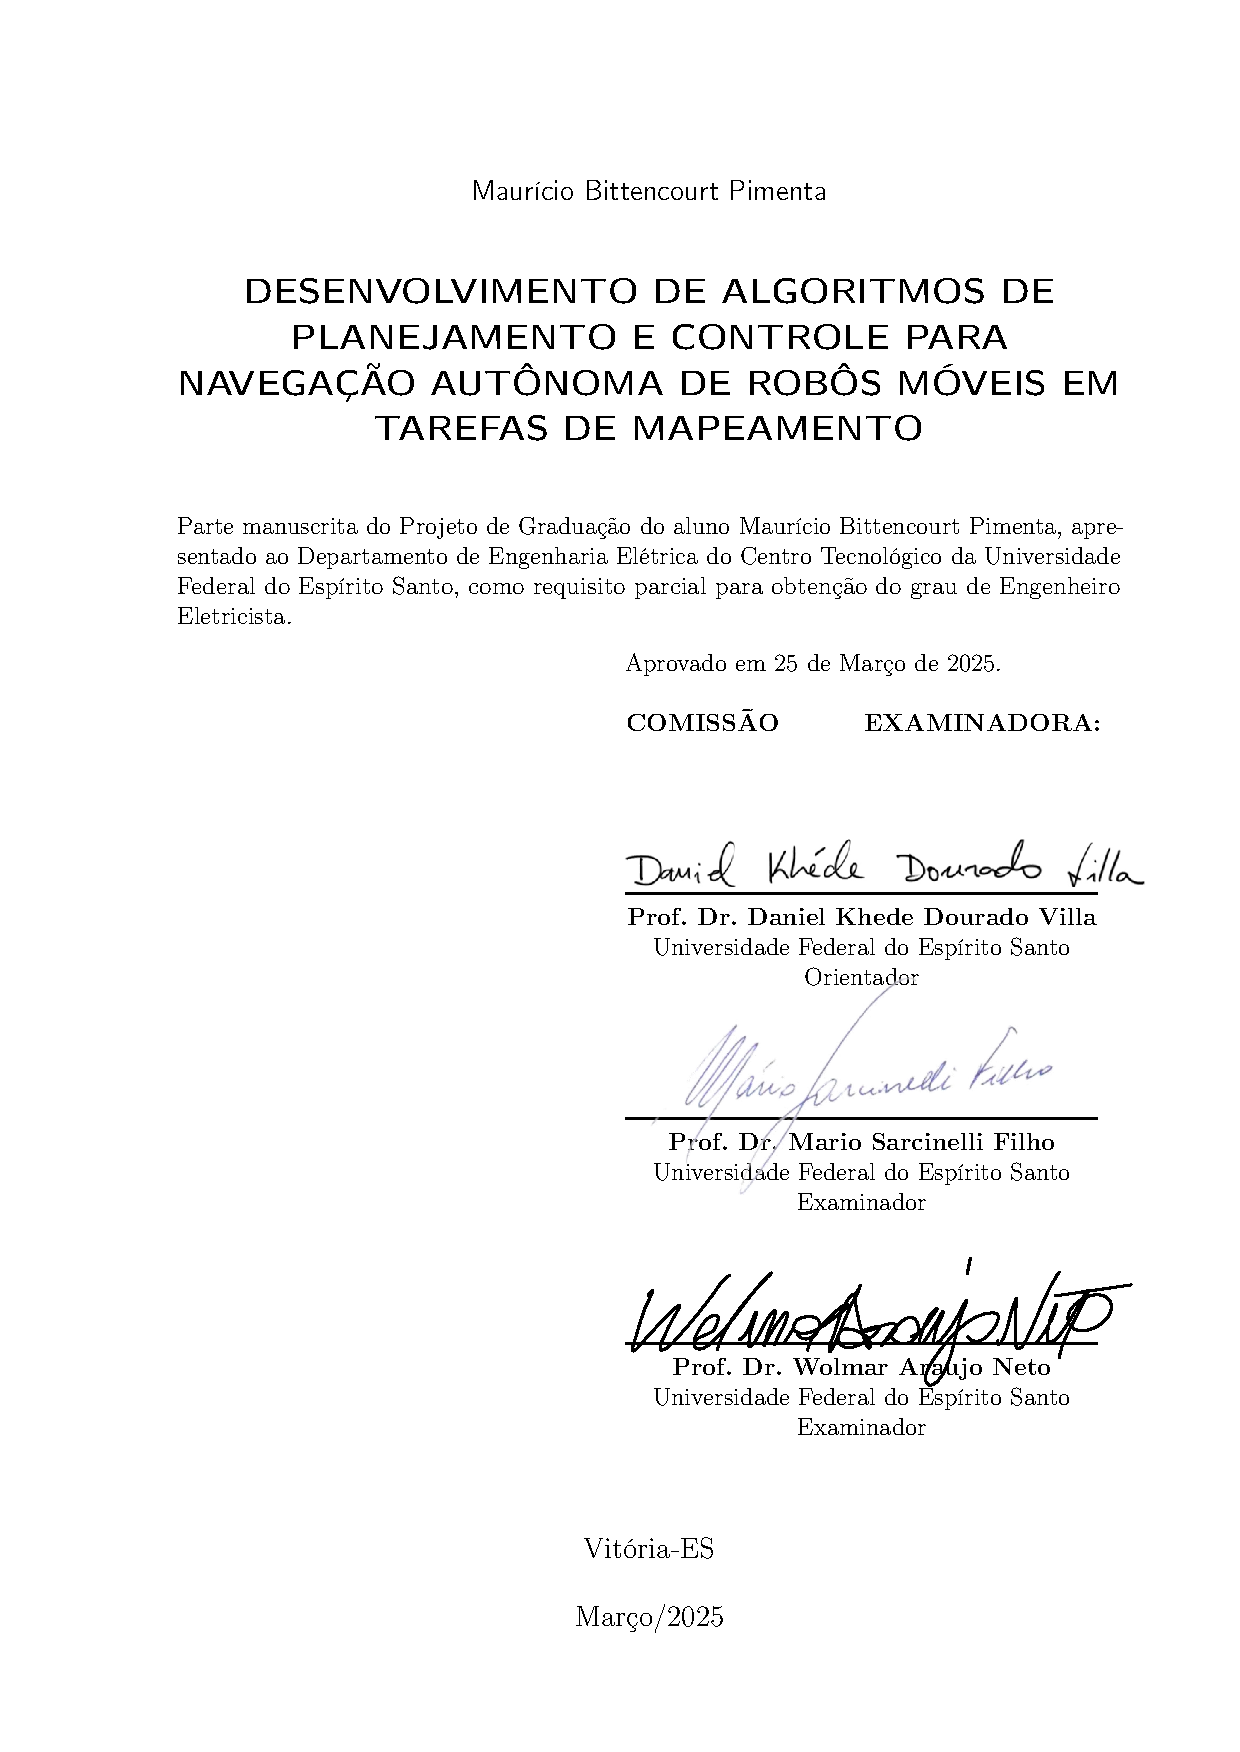
\includepdf{aprovacao.pdf}

 \begin{folhadeaprovacao}
   \begin{center}
     {\ABNTEXchapterfont\large\imprimirautor}
 	\begin{center}
      	\ABNTEXchapterfont\bfseries\Large\imprimirtitulo
     \end{center}
     %\vspace*{\fill}
   \end{center}    
     \imprimirpreambulo
 		\vspace{-0.5cm}
     \begin{center}
 		\hspace{.45\textwidth}
     \begin{minipage}{.5\textwidth}
%         \textbf{COMISSÃO EXAMINADORA:}
\assinatura{\textbf{Profa. Dra. Marcia Helena Moreira Paiva} \\ Universidade Federal do Espírito Santo \\ Professor da Disciplina}
\assinatura{\textbf{\imprimirorientador} \\ Universidade Federal do Espírito Santo \\ Orientador} 
\assinatura{\textbf{\imprimircoorientador} \\ Universidade Federal do Espírito Santo \\ Coorientadora}
\assinatura{\textbf{\imprimirautor} \\ Universidade Federal do Espírito Santo \\ Aluno}
% 		\assinatura{\textbf{Prof. Dr. Pedro Pedrinho} \\ Universidade Federal do Espírito Santo \\ Examinador}
% 		\assinatura{\textbf{Msc. João da Vida} \\ Universidade Federal do Espírito Santo \\ Examinador}
     \end{minipage}
 	    \vspace*{\fill}
    \end{center}
         
    \begin{center}
       	% >> Se necessáiro, ajustar os \vspace
 		%\vspace*{0.5cm}
     	{\large\imprimirlocal}
     	\par
     	{\large\imprimirdata}
    		%\vspace*{1cm}
   \end{center}  
 \end{folhadeaprovacao}
 
 
 % --------------------------------------------------- %
%						Resumo				      	  %	
% --------------------------------------------------- %

% Resumo em português
\setlength{\absparsep}{18pt} % ajusta o espaçamento dos parágrafos do resumo
\begin{resumo}

{\sffamily This is a sample text in \textbf{Sans Serif Font Typeface}}
Identifica qual é a grande área onde seu trabalho esta inserido e qual é a importância dessa grande área.
\textbf{2. \txr{Gaps ou vazios}}
Aqui o autor diz que coisa na grande área precisa ser pesquisada. 
Aqui é onde o autor deixa claro o que ainda não esta bem entendido, esta em aberto ou é controvertido. 
Em resumo, o Gap é o vazio dessa grande área na qual  o trabalho esta inserido. 
O comum é iniciar con as palavras: \textit{ainda}, \textit{Sem embargo}
\textbf{\txr{3. Proposta}}
Em esta parte o autor indica qual é o proposta e o objetivo do trabalho, evidentemente o objetivo deve estar relacionado con el Gap. O comum é iniciar con as frases: \textit{Este trabalho descreve ...}; \textit{Este trabalho reporta ...}; \textit{Aqui, ...}; \textit{Em este trabalho, é proposto, ... }.
\textbf{\txr{4. Metodologia}}
Aqui são descritos os métodos utilizados para a realização do trabalho.
\textbf{\txr{5. Resultados}}
Esta parte do resumo é extremadamente importante, não existe resumo que não tenha seção de resultados bem clara e detalhada, cabe ao autor identificar qual é seu principal resultado, para deixar bem claro no resumo.  Acontinuação um exemplo.

\textbf{1. \txr{Contextualização}}
O câncer de pele é o tipo de câncer mais comum no Brasil. 
O melanoma é seu subtipo mais mortal. 
Portanto, é essencial que seja detectado em seus estágios iniciais, quando a taxa de sobrevivência ainda é alta. 
Entretanto, ele é muito fácil de ser confundido por pintas comuns ou outros tipos de lesões de pele, até mesmo por especialistas. 
\textbf{2. \txr{Gaps ou vazios}}
Assim, alguma ferramenta de diagnóstico automatizado se torna indispensável. 
Porém, as soluções automatizadas existentes não são muito superiores aos diagnósticos comuns. 
A partir de $2012$ houveram grandes avanços na aplicação de redes neurais para a classificação de imagens. 
A aplicação de redes neurais convolucionais profundas está superando a performance humana em diversas tarefas. 
\textbf{3. \txr{Proposta}}
O presente projeto de graduação faz uso de uma rede convolucional para tentar solucionar o problema de classificação binária de imagens de melanomas ou ceratoses seborréicas contra nevos. 
A tarefa a solucionar foi obtida do desafio ISIC 2017, que provê um banco de dados para realizar o treino das redes e para validar a solução. 
\textbf{4. \txr{Metodologia}}
Para auxiliar e facilitar a tarefa foram usadas as técnicas de pré-processamento de imagens e transferência de aprendizado. 
Um estudo aprofundado é feito sobre a arquitetura da rede usada, detalhando seu funcionamento interno. São treinados diversos classificadores para a tarefa dos quais o melhor obteve um desempenho equiparável a soluções de outras equipes. 
\textbf{5. \txr{Resultados}}
Especificamente, é obtido uma média de área sob a curva de característica de operação do receptor de $0.877$ quando testado no banco de dados do desafio ISIC 2017, ficando situado entre os 10 melhores resultados.

\textbf{Palavras-chave}: \textit{Deep-learning}; Redes neurais convolucionais; \textit{Transfer-learning}.
\end{resumo}

% --------------------------------------------------- %
%					Resumo em ingles	      	  	  %	
% --------------------------------------------------- %
\begin{resumo}[Abstract]
 \begin{otherlanguage*}{english}
   \noindent xxxxx.
   
   \textbf{Keywords}: xxxx; yyyy.
 \end{otherlanguage*}
\end{resumo}
\else   % TCC
    % --------------------------------------------------- %
%						Capa						  %
% --------------------------------------------------- %
% >>> Capa Personalizada
\renewcommand{\imprimircapa}{%
	\begin{capa}%
		\center
		{\ABNTEXchapterfont\bfseries\large\imprimirINSTITUICAO}
			\vspace*{1.5cm}
		\includegraphics*[width=0.25\textwidth]{brasao_ufes.jpg}
			\vspace*{1.5cm} \\
		{\ABNTEXchapterfont\bfseries\Large\MakeUppercase\imprimirautor}
				\vspace*{2.5cm} \\
		{\ABNTEXchapterfont\bfseries\Large\imprimirtitulo}
			\vfill
			\vspace*{0.5cm}
		{\large\MakeUppercase\imprimirlocal}
		\par
		{\large\MakeUppercase\imprimirdata}
			\vspace*{1cm}
	\end{capa}
}

\imprimircapa

% --------------------------------------------------- %
%					Folha de Rosto 					  %
% --------------------------------------------------- %
% >> O * indica que haverá a ficha bibliográfica

\renewcommand{\imprimirfolhaderosto}{

\begin{folhaderosto}
	\begin{center}
    	{\ABNTEXchapterfont\large\imprimirautor}
		    \vspace*{\fill}\vspace*{\fill}
    	\begin{center}
	    	\ABNTEXchapterfont\bfseries\Large\imprimirtitulo
	    \end{center}
    		\vspace*{\fill}
    		\hspace{.45\textwidth}
	    \begin{minipage}{.5\textwidth}
        	\imprimirpreambulo
	    \end{minipage}
    		\vspace*{\fill}
	    \end{center}  
        \begin{center}
        	% >> Se necessáiro, ajustar os \vspace
        	%\vspace*{0.5cm}
        {\large\imprimirlocal}
        \par
        {\large\imprimirdata}
       		%\vspace*{1cm}
      \end{center}
\end{folhaderosto}
}

\imprimirfolhaderosto

% --------------------------------------------------- %
%					Ficha Catalográfica 			  %
% --------------------------------------------------- %

% Isto é um exemplo de Ficha Catalográfica, ou ``Dados internacionais de
% catalogação-na-publicação''. Você pode utilizar este modelo como referência. 
% Porém, provavelmente a biblioteca da sua universidade lhe fornecerá um PDF
% com a ficha catalográfica definitiva após a defesa do trabalho. Quando estiver
% com o documento, salve-o como PDF no diretório do seu projeto e substitua todo
% o conteúdo de implementação deste arquivo pelo comando abaixo:
%
% \begin{fichacatalografica}
%     \includepdf{fig_ficha_catalografica.pdf}
% \end{fichacatalografica}

%\begin{fichacatalografica}
%	\sffamily
%	\vspace*{\fill}					% Posição vertical
%	\begin{center}					% Minipage Centralizado
%	\fbox{\begin{minipage}[c][8cm]{13.5cm}		% Largura
%	\small
%	\imprimirautor
%	%Sobrenome, Nome do autor
%	
%	\hspace{0.5cm} \imprimirtitulo  / \imprimirautor. --
%	\imprimirlocal, \imprimirdata-
%	
%	\hspace{0.5cm} \pageref{LastPage} p. : il. (algumas color.) ; 30 cm.\\
%	
%	\hspace{0.5cm} \imprimirorientadorRotulo~\imprimirorientador\\
%	
%	\hspace{0.5cm}
%	\parbox[t]{\textwidth}{\imprimirtipotrabalho~--~\imprimirinstituicao,
%	\imprimirdata.}\\
%	
%	\hspace{0.5cm}
%		1. Palavra-chave1.
%		2. Palavra-chave2.
%		2. Palavra-chave3.
%		I. Orientador.
%		II. Universidade xxx.
%		III. Faculdade de xxx.
%		IV. Título 			
%	\end{minipage}}
%	\end{center}
%\end{fichacatalografica}

% --------------------------------------------------- %
%					Folha de Aprovação			      %
% --------------------------------------------------- %
% >>> Após apresentação do trabalho, substitua todo o conteúdo 
% por uma imagem da página assinada pela banca com o comando abaixo:
\ifisFolhaAprovacao
%TCC finalizado
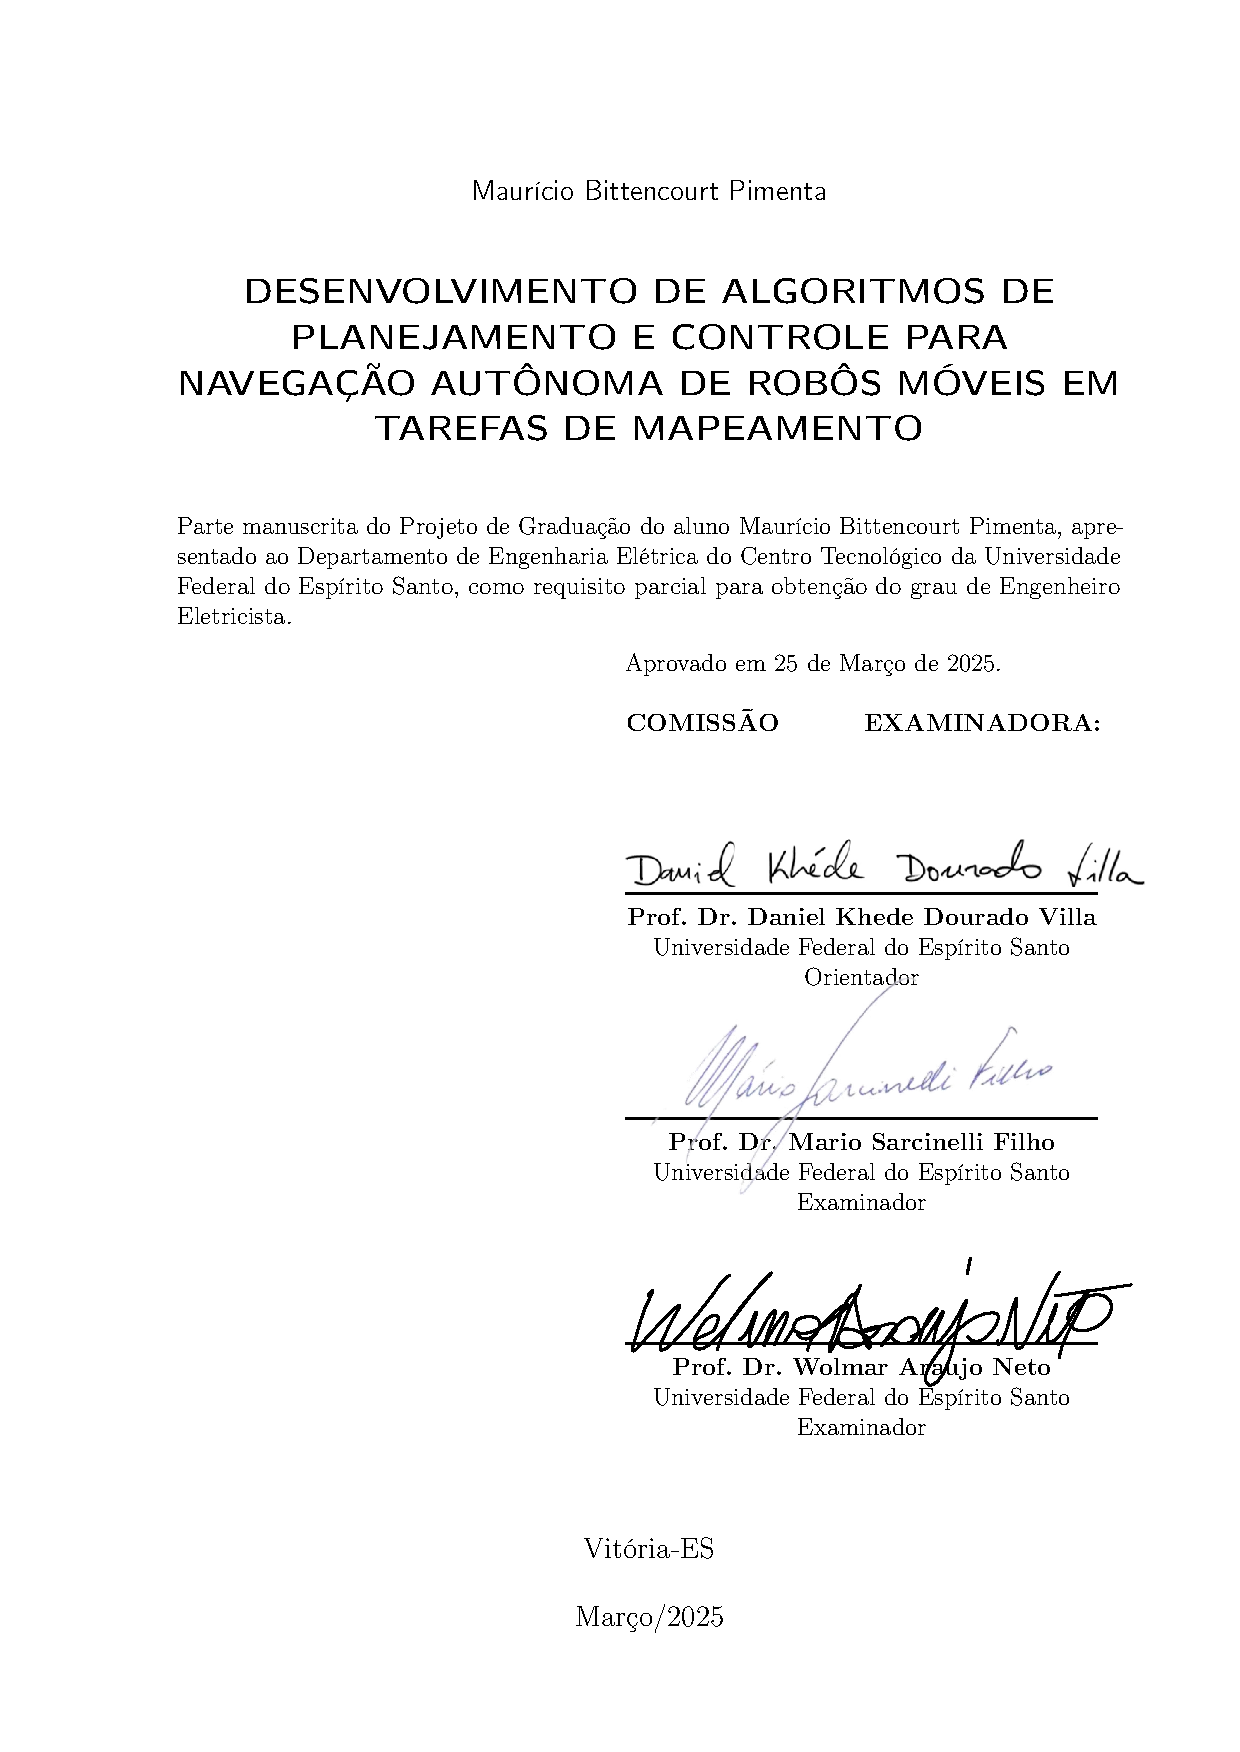
\includepdf{aprovacao.pdf}
\else
%TCC não finalizado
\begin{folhadeaprovacao}
   \begin{center}
     {\ABNTEXchapterfont\large\imprimirautor}
 	\begin{center}
      	\ABNTEXchapterfont\bfseries\Large\imprimirtitulo
     \end{center}
     %\vspace*{\fill}
   \end{center}    
     \imprimirpreambulo
 		\vspace{-0.5cm}
     \begin{center}
 		\hspace{.45\textwidth}
     \begin{minipage}{.5\textwidth}
         Aprovado em x de xxxx de 20xx. \\\\
         \textbf{COMISSÃO EXAMINADORA:}
         \vspace{0.5cm}
         \assinatura{\textbf{\imprimirorientador} \\ Universidade Federal do Espírito Santo \\ Orientador}
         %\vspace{1.0cm}
%        \assinatura{\textbf{\imprimircoorientador} \\ Universidade Federal do Espírito Santo \\ Coorientadora}
        \vspace{1.0cm}
 		\assinatura{\textbf{Prof. Dr. Mario Sarcinelli Filho} \\ Universidade Federal do Espírito Santo \\ Examinador}
 		\vspace{1.0cm}
 		\assinatura{\textbf{Prof. Dr. Wolmar Araujo Neto} \\ Universidade Federal do Espírito Santo \\ Examinador}
     \end{minipage}
 	    \vspace*{\fill}
    \end{center}
         
    \begin{center}
       	% >> Se necessáiro, ajustar os \vspace
 		%\vspace*{0.5cm}
     	{\large\imprimirlocal}
     	\par
     	{\large\imprimirdata}
    		%\vspace*{1cm}
   \end{center}  
 \end{folhadeaprovacao}
\fi
% --------------------------------------------------- %
%						Dedicatória				      %
% --------------------------------------------------- %
\begin{dedicatoria}
   \vspace*{\fill}
   \centering
   \noindent
   \textit{Dedicatória!!} \vspace*{\fill}
\end{dedicatoria}

% --------------------------------------------------- %
%					Agradecimentos				      %
% --------------------------------------------------- %

\begin{agradecimentos}

% Gostaria de agradecer a todas essas pessoas especiais que apareceram (e estão) na minha vida e que permitem que eu continue com os meus estudos. A todos vocês, minha eterna gratidão.

% Aos meus pais, Adan e Eva, pelo apoio e dedicação e xxxx.
    
% Ao minha/meu irmã@ Mari@ por todo apoio emocional e por me servir de inspiração.

% À minha/meu namorad@ Mari@ por toda compreensão e apoio durante toda a graduação.
    	
% A meu orientador Yann Lecun e coorientador Geoffrey Hinton por despertar meu interesse por esse tema fascinante e por toda ajuda, orientação e dedicação durante o desenvolvimento deste trabalho.

% Aos membros do Laboratório Visio, pelo xxxx.

% À banca examinadora pela aceitação do convite e pelo tempo investido para leitura e avaliação desse trabalho.

% Agradeço à Universidade Federal do Espirito Santo pela minha formação. 

% Finalmente, agradeço à Fundação de XXXX pelo apoio financeiro.
\end{agradecimentos}

% --------------------------------------------------- %
%						Epígrafe			      	  %	
% --------------------------------------------------- %

%\begin{epigrafe}
%    \vspace*{\fill}
%	\begin{flushright}
%		Insira a epígrafe aqui!
%	\end{flushright}
%\end{epigrafe}

% --------------------------------------------------- %
%						Resumo				      	  %	
% --------------------------------------------------- %

% Resumo em português
\setlength{\absparsep}{18pt} % ajusta o espaçamento dos parágrafos do resumo
\begin{resumo}

% \txr{\textbf{COMENTARIO GERAL:}} O resumo de um trabalho tem uma estrutura bem definida, explicada a seguir:
% \textbf{1. \txr{Contextualização}}
% Identifica qual é a grande área onde seu trabalho esta inserido e qual é a importância dessa grande área.
% \textbf{2. \txr{Gaps ou vazios}}
% Aqui o autor diz que coisa na grande área precisa ser pesquisada. 
% Aqui é onde o autor deixa claro o que ainda não esta bem entendido, esta em aberto ou é controvertido. 
% Em resumo, o Gap é o vazio dessa grande área na qual  o trabalho esta inserido. 
% O comum é iniciar con as palavras: \textit{ainda}, \textit{Sem embargo}
% \textbf{\txr{3. Proposta}}
% Em esta parte o autor indica qual é o proposta e o objetivo do trabalho, evidentemente o objetivo deve estar relacionado con el Gap. O comum é iniciar con as frases: \textit{Este trabalho descreve ...}; \textit{Este trabalho reporta ...}; \textit{Aqui, ...}; \textit{Em este trabalho, é proposto, ... }.
% \textbf{\txr{4. Metodologia}}
% Aqui são descritos os métodos utilizados para a realização do trabalho.
% \textbf{\txr{5. Resultados}}
% Esta parte do resumo é extremadamente importante, não existe resumo que não tenha seção de resultados bem clara e detalhada, cabe ao autor identificar qual é seu principal resultado, para deixar bem claro no resumo.  Acontinuação um exemplo.

% \textbf{1. \txr{Contextualização}}
% O câncer de pele é o tipo de câncer mais comum no Brasil. 
% O melanoma é seu subtipo mais mortal. 
% Portanto, é essencial que seja detectado em seus estágios iniciais, quando a taxa de sobrevivência ainda é alta. 
% Entretanto, ele é muito fácil de ser confundido por pintas comuns ou outros tipos de lesões de pele, até mesmo por especialistas. 
% \textbf{2. \txr{Gaps ou vazios}}
% Assim, alguma ferramenta de diagnóstico automatizado se torna indispensável. 
% Porém, as soluções automatizadas existentes não são muito superiores aos diagnósticos comuns. 
% A partir de $2012$ houveram grandes avanços na aplicação de redes neurais para a classificação de imagens. 
% A aplicação de redes neurais convolucionais profundas está superando a performance humana em diversas tarefas. 
% \textbf{3. \txr{Proposta}}
% O presente projeto de graduação faz uso de uma rede convolucional para tentar solucionar o problema de classificação binária de imagens de melanomas ou ceratoses seborréicas contra nevos. 
% A tarefa a solucionar foi obtida do desafio ISIC 2017, que provê um banco de dados para realizar o treino das redes e para validar a solução. 
% \textbf{4. \txr{Metodologia}}
% Para auxiliar e facilitar a tarefa foram usadas as técnicas de pré-processamento de imagens e transferência de aprendizado. 
% Um estudo aprofundado é feito sobre a arquitetura da rede usada, detalhando seu funcionamento interno. São treinados diversos classificadores para a tarefa dos quais o melhor obteve um desempenho equiparável a soluções de outras equipes. 
% \textbf{5. \txr{Resultados}}
% Especificamente, é obtido uma média de área sob a curva de característica de operação do receptor de $0.877$ quando testado no banco de dados do desafio ISIC 2017, ficando situado entre os 10 melhores resultados.

% A autonomia de robôs móveis terrestres é fundamental em diversas aplicações, como exploração, vigilância e mapeamento de ambientes, permitindo que máquinas operem sem intervenção humana direta. Em tarefas cooperativas de mapeamento envolvendo múltiplos robôs, a navegação autônoma eficiente e precisa torna-se ainda mais importante para assegurar cobertura completa da área e a alta qualidade dos mapas gerados. No entanto, a realização eficaz dessas tarefas enfrenta vários desafios. Ainda é necessário aprimorar algoritmos que planejem rotas de mapeamento ótimas, cobrindo a região alvo com deslocamento mínimo. Adicionalmente, a fusão dos mapas produzidos por cada robô requer técnicas robustas para evitar distorções, e é crucial manter uma estimativa confiável da pose (localização) de cada robô durante a navegação em ambientes inicialmente desconhecidos ou dinâmicos. 
% Este trabalho apresenta o desenvolvimento e a validação experimental de algoritmos de planejamento de trajetórias e controle cinemático para um robô móvel diferencial, visando viabilizar sua navegação autônoma em tarefas de mapeamento. A abordagem proposta integra técnicas de SLAM (Simultaneous Localization and Mapping) — por meio da biblioteca SLAM Toolbox do ROS — de forma que o robô estime continuamente sua própria pose e construa um mapa 2D do ambiente em tempo real enquanto segue rotas pré-definidas. 
% Na metodologia, empregou-se a plataforma robótica LIMO (um robô móvel de tração diferencial equipado com sensor LiDAR 2D) e implementou-se um controlador cinemático de seguimento de trajetória e rotinas de planejamento de rotas, além da integração da SLAM Toolbox para geração do mapa ocupacional e estimativa da pose durante a navegação. Um sistema de captura de movimento OptiTrack foi utilizado como referência externa de alta precisão (ground truth) da posição do robô, possibilitando avaliar a acurácia da localização provida pelo SLAM. Experimentos em ambiente de laboratório foram conduzidos com o robô percorrendo diferentes trajetórias (uma sequência de segmentos retos, denominada “CASA”, e uma curva fechada no formato de lemniscata de Bernoulli) sob duas condições de localização: (i) usando a pose fornecida pelo OptiTrack como referência ideal, e (ii) usando exclusivamente a pose estimada pelo SLAM. Assim, pôde-se comparar o desempenho do seguimento de trajetória com e sem o auxílio da localização via SLAM. 
% Os resultados experimentais demonstraram que o sistema desenvolvido é capaz de guiar o robô pelo ambiente de forma autônoma, mapeando-o simultaneamente. Em ambas as trajetórias de teste, o robô seguiu o caminho desejado com sucesso. No cenário com localização via OptiTrack, o seguimento de trajetória apresentou alta precisão, com apenas pequenos erros em curvas mais fechadas e no início do movimento. Já no cenário usando apenas a pose estimada pela SLAM Toolbox, o robô também completou as rotas planejadas, porém observou-se um aumento nos erros de rastreamento e um leve comportamento oscilatório em certos trechos, especialmente ao executar a curva em formato de lemniscata. Apesar dessas diferenças, as trajetórias estimadas pelo SLAM mantiveram-se próximas das medidas pela referência externa, indicando que a estimação de pose via SLAM foi, em geral, confiável. Em suma, o sistema proposto mostrou-se eficaz para a navegação e mapeamento autônomo em um ambiente real de laboratório, demonstrando o potencial dos algoritmos desenvolvidos para futuras aplicações de mapeamento cooperativo multi-robôs.

A autonomia de robôs móveis terrestres é essencial em uma variedade de aplicações, como exploração de ambientes desconhecidos, vigilância e mapeamento de áreas de difícil acesso. Em tarefas cooperativas de mapeamento, onde múltiplos robôs trabalham simultaneamente, é crucial garantir que a navegação seja eficiente e que a área seja coberta de maneira completa, sem sobreposição de trajetórias. Além disso, a precisão no mapeamento e a fusão de mapas gerados por diferentes robôs são desafios importantes. A realização dessas tarefas em ambientes dinâmicos ou inicialmente desconhecidos exige o uso de técnicas robustas de localização e planejamento de trajetórias. Este trabalho apresenta o desenvolvimento e a validação experimental de algoritmos para o controle de navegação autônoma de robôs móveis em tarefas de mapeamento cooperativo. A proposta integra o uso da SLAM Toolbox do ROS para a estimativa de pose e a geração de mapas 2D, enquanto o robô segue trajetórias predefinidas no ambiente. O robô LIMO, com tração diferencial e equipado com um sensor LiDAR 2D, foi utilizado como plataforma experimental. A metodologia inclui a implementação de um controlador cinemático baseado em algoritmos de controle de seguimento de trajetória, que utiliza a estimativa de pose provida pelo sistema SLAM para guiar o robô ao longo do caminho planejado. Para validar a precisão do sistema, foi empregado o sistema de captura de movimento OptiTrack como referência de alta precisão (ground truth). Os experimentos realizados consistiram em testar duas trajetórias: uma sequência de segmentos retos, chamada "CASA", e uma curva em formato de lemniscata de Bernoulli. Nos testes, o robô foi capaz de seguir as trajetórias planejadas de forma satisfatória. Nos cenários em que a localização foi obtida com o sistema OptiTrack, a precisão foi alta, com pequenos erros em pontos de virada. Quando a localização foi fornecida apenas pelo SLAM, o robô também completou as trajetórias, mas com um desempenho levemente inferior, apresentando erros maiores e oscilações em trechos mais críticos. Apesar dessas oscilações, a estimação de pose fornecida pela SLAM Toolbox mostrou-se bastante confiável, permitindo uma navegação efetiva no ambiente de laboratório. O trabalho conclui que a integração de controle cinemático com SLAM oferece uma solução robusta e eficaz para navegação autônoma e mapeamento em ambientes reais, com perspectivas de aplicação em sistemas de mapeamento cooperativo multi-robôs.

\textbf{Palavras-chave}: Robótica móvel; Navegação autônoma; SLAM; Planejamento de trajetórias.
\end{resumo}

% --------------------------------------------------- %
%					Resumo em ingles	      	  	  %	
% --------------------------------------------------- %
\begin{resumo}[Abstract]
 \begin{otherlanguage*}{english}
   % The autonomy of ground mobile robots is crucial in various applications such as exploration, surveillance, and environmental mapping, enabling machines to operate without direct human intervention. In cooperative mapping missions involving multiple robots, achieving efficient and accurate autonomous navigation becomes even more critical to ensure complete area coverage and high-quality map generation. However, accomplishing these tasks effectively still poses several challenges. It remains necessary to improve algorithms that plan optimal mapping routes, covering target regions with minimal redundant motion. In addition, merging the maps produced by each robot requires robust techniques to avoid distortions, and maintaining a reliable estimate of each robot’s pose during navigation in initially unknown or dynamic environments is essential. This work presents the development and experimental validation of trajectory planning and kinematic control algorithms for a differential mobile robot, aiming to enable its autonomous navigation in mapping tasks. The proposed approach integrates SLAM (Simultaneous Localization and Mapping) techniques — using the ROS SLAM Toolbox — so that the robot can continuously estimate its own pose and build a 2D map of the environment in real time while following predefined routes. The methodology employed the LIMO robotic platform (a differential-drive mobile robot equipped with a 2D LiDAR sensor) and the ROS framework for software integration. A kinematic trajectory-following controller and route planning routines were implemented, alongside the integration of SLAM Toolbox for occupancy grid mapping and pose estimation during navigation. An OptiTrack motion capture system provided a high-precision external reference (ground truth) for the robot’s position, enabling evaluation of the accuracy of the SLAM-based localization. Laboratory experiments were conducted with the robot traversing different trajectories (a sequence of straight-line segments nicknamed “CASA”, and a closed Bernoulli lemniscate curve) under two localization conditions: (i) using the OptiTrack-provided pose as an ideal reference, and (ii) using exclusively the pose estimated by SLAM. This setup allowed a comparative assessment of trajectory tracking performance with and without SLAM-based localization. The experimental results demonstrated that the developed system can autonomously guide the robot through the environment while simultaneously mapping it. In both test trajectories, the robot successfully followed the desired path. In the scenario with OptiTrack localization, trajectory tracking was highly accurate, with only minor errors at sharper turns and at the start of motion. In the scenario using only the pose from the SLAM Toolbox, the robot also completed the planned routes, but an increase in tracking errors and a slight oscillatory behavior were observed in certain segments, especially when executing the lemniscate curve. Despite these differences, the trajectories estimated by SLAM remained close to those measured by the external reference, indicating that the SLAM-based pose estimation was generally reliable. In summary, the proposed system proved effective for autonomous navigation and mapping in a real laboratory environment, demonstrating the potential of the developed algorithms for future multi-robot cooperative mapping applications.

    The autonomy of ground mobile robots plays a key role in a variety of applications, such as exploration of unknown environments, surveillance, and mapping of hard-to-access areas. In cooperative mapping tasks, where multiple robots work simultaneously, it is crucial to ensure efficient navigation and complete area coverage without trajectory overlap. Furthermore, mapping accuracy and the fusion of maps generated by different robots present significant challenges. Performing these tasks in dynamic or initially unknown environments requires robust techniques for localization and trajectory planning. This work presents the development and experimental validation of algorithms for autonomous navigation control in mobile robots for cooperative mapping tasks. The proposed approach integrates the use of the ROS SLAM Toolbox for pose estimation and 2D map generation, while the robot follows predefined paths in the environment. The LIMO robot platform, with differential drive and equipped with a 2D LiDAR sensor, was used for experimentation. The methodology includes implementing a kinematic controller based on trajectory following control algorithms, utilizing the pose estimation provided by the SLAM system to guide the robot along the planned path. To validate the system’s accuracy, the OptiTrack motion capture system was used as a high-precision reference (ground truth). The experiments involved testing two different trajectories: a sequence of straight-line segments, called “CASA”, and a Bernoulli lemniscate curve. In the tests, the robot was able to follow the planned trajectories satisfactorily. In scenarios where localization was provided by the OptiTrack system, high precision was achieved with only small errors at turning points. When localization was provided only by SLAM, the robot still completed the trajectories, but with slightly worse performance, showing larger errors and oscillations in more critical segments. Despite these oscillations, the pose estimation provided by the SLAM Toolbox proved to be reliable, enabling effective navigation in the laboratory environment. This work concludes that the integration of kinematic control with SLAM provides a robust and effective solution for autonomous navigation and mapping in real environments, with potential applications in multi-robot cooperative mapping systems.
   
   \textbf{Keywords}: Mobile robotics; Autonomous navigation; SLAM; Trajectory planning.
 \end{otherlanguage*}
\end{resumo}
\fi
%%%%%%%
 
% --------------------------------------------------- %
%					Lista de Figuras	      	  	  %	
% --------------------------------------------------- %
\renewcommand{\listfigurename}{Lista de Figuras}
\listoffigures*
\cleardoublepage

% --------------------------------------------------- %
%					Lista de Tabelas				  %	
% --------------------------------------------------- %

\pdfbookmark[0]{\listtablename}{lot}
\listoftables*
\cleardoublepage

% --------------------------------------------------- %
%					Lista de Quadros				  %	
% --------------------------------------------------- %

%\pdfbookmark[0]{\listofquadrosname}{loq}
%\listofquadros*
%\cleardoublepage

% --------------------------------------------------- %
%			Lista de Abreviaturas e Siglas			  %	
% --------------------------------------------------- %
\begin{siglas}
%%%%%%%%%%%%%  A %%%%%%%%%%%%%%%
%%%%%%%%%%%%%  B %%%%%%%%%%%%%%%
%%%%%%%%%%%%%  C %%%%%%%%%%%%%%%
% \item[CNN] \textit{Convolutional Neural Network}
%%%%%%%%%%%%%  D %%%%%%%%%%%%%%%
% \item [DL] \textit{Deep Learning}
%%%%%%%%%%%%%  E %%%%%%%%%%%%%%%
\item[ESC] Controladores Eletrônicos de Velocidade
\item[EKF] \textit{Extended Kalman Filter} - Filtro de Kalman Extendido
%%%%%%%%%%%%%  F %%%%%%%%%%%%%%%
\item[FastSLAM] Localização e Mapeamento Simultâneos utilizando a técnica de Filtro de Partículas
%%%%%%%%%%%%%  G %%%%%%%%%%%%%%%
\item[GPU] \textit{Graphics Processing Unit} 
%%%%%%%%%%%%%  H %%%%%%%%%%%%%%%
%%%%%%%%%%%%%  I %%%%%%%%%%%%%%%
\item[IMU]  Unidade de Medição Inercial (\textit{Inertial Measurement Unit})
%%%%%%%%%%%%%  J %%%%%%%%%%%%%%%
%%%%%%%%%%%%%  K %%%%%%%%%%%%%%%
\item[KF] \textit{Kalman Filter} - Filtro de Kalman
%%%%%%%%%%%%%  L %%%%%%%%%%%%%%%
\item[LAB-AIR] Laboratório de Automação Inteligente e Robótica
\item[LiDAR] \textit{Light Detection And Ranging}
%%%%%%%%%%%%%  M %%%%%%%%%%%%%%%
% \item[ML] \textit{Machine Learning}
%%%%%%%%%%%%%  N %%%%%%%%%%%%%%%
%%%%%%%%%%%%%  O %%%%%%%%%%%%%%%
%%%%%%%%%%%%%  P %%%%%%%%%%%%%%%
%%%%%%%%%%%%%  Q %%%%%%%%%%%%%%%
%%%%%%%%%%%%%  R %%%%%%%%%%%%%%%
%%%%%%%%%%%%%  S %%%%%%%%%%%%%%%
\item[SLAM] \textit{Simultaneous Localization and Mapping}
% \item[SGD] \textit{Stochastic Gradient Descent}
%%%%%%%%%%%%%  T %%%%%%%%%%%%%%%
%%%%%%%%%%%%%  U %%%%%%%%%%%%%%%
\item[UFES] Universidade Federal do Espírito Santo
%%%%%%%%%%%%%  V %%%%%%%%%%%%%%%
%%%%%%%%%%%%%  W %%%%%%%%%%%%%%%
%%%%%%%%%%%%%  Y %%%%%%%%%%%%%%%
%%%%%%%%%%%%%  Z %%%%%%%%%%%%%%%
\end{siglas}

% --------------------------------------------------- %
%					Lista de Símbolos				  %	
% --------------------------------------------------- %

%\begin{simbolos}
%	\item[]
%\end{simbolos}

% --------------------------------------------------- %
%						Sumário						  %	
% --------------------------------------------------- %

\pdfbookmark[0]{\contentsname}{toc}
\tableofcontents*
\cleardoublepage

% --------------------------------------------------- %
%					Elementos Textuais				  %
% --------------------------------------------------- %

\textual

\chapter[Introdução]{Introdução}
% CHAPTER 01 - INTRODUÇÃO
%
%
% Ajustar esse \vspace de acordo com o necessário
\vspace{-42pt}

A crescente demanda por sistemas de transporte autônomos e eficientes impulsionou o desenvolvimento de tecnologias inovadoras no campo da robótica e da inteligência artificial \cite{Chen2023MilestonesSurveys} \cite{Teng2023MotionPerspectives}. Em específico, muito se discute do uso de veículos autônomos para a entrega de pacotes e transporte autônomo de cargas. \cite{Bacheti2022Leader-FollowerDelivery} \cite{Vale2021VeiculoIndustrial} \cite{Bacheti2021ALast-Mile-Delivery}
Em geral, assume-se na literatura que o transporte de cargas ocorre em ambiente estruturado, previamente conhecido. No entanto, o alevar esta tecnologia da academia para o mundo real, não necessariamente isso será uma realidade. Por vezes, o transporte terá um destino em que apenas uma breve descrição da estrutura local será apresentada para o sistema. Sendo assim, sistemas que visam a realização do transporte autônomo de cargas por robôs móveis se beneficiam de subsistemas de localização e mapeamento.\cite{Cadena2016PastAge}

Neste contexto, a cooperação entre robôs móveis aéreos e terrestres tem se destacado como uma abordagem promissora para a realização de tarefas complexas de navegação autônoma e mapeamento. A principal vantagem de mapear uma área de forma cooperativa está na capacidade de cobrir uma área maior em menos tempo. Ao utilizar um sistema multirrobô para mapeamento, pode-se trabalhar simultaneamente em áreas diferentes, aumentando a eficiência do mapeamento\cite{Feng2020AnSystems}. Além disso, a combinação das habilidades complementares dos veículos aéreos e terrestres oferece vantagens significativas no cumprimento desta tarefa, permitindo a realização de operações com maior eficiência e flexibilidade \cite{Bacheti2022Leader-FollowerDelivery}. Outra vantagem dessa cooperação é o mapeamento em terrenos complexos, como áreas urbanas ou locais de difícil acesso. A utilização de veículos aéreos para capturar imagens e dados tridimensionais do ambiente, combinada com a capacidade dos veículos terrestres de navegar de forma precisa e interagir com o terreno, pode fornecer informações detalhadas para a construção de mapas atualizados e de alta resolução.

Apesar das vantagens, a realização de tarefas de mapeamento de forma cooperativa apresenta diversos desafios. Primeiramente, se faz necessário que os robôs sigam uma rota eficiente para o mapeamento, fazendo com que estes precisem realizar menos movimentos para cobrir toda a área a ser mapeada.  Mais ainda, os mapas gerados individualmente pelos robôs devem ser combinados em um único mapa, com o cuidade para que o algoritmo não gere distorções geométricas, artefatos, ou sofra com variações de resolução, escala e iluminação \cite{Bavle2023FromSurvey}\cite{AbaspurKazerouni2022ASLAM}. Por fim, é importante que os robôs sejam capazes de desviar de obstáculos em ambientes estáticos, e de outros agentes de forma ágil em ambientes dinâmicos \cite{Li2022VisualDetection}. Esses requisitos exigem um planejamento ótimo para as rotas de navegação cooperativa\cite{Vasconcelos2020Real-timeMissions}.


\section{Objetivos}

\paragraph*{Objetivo Geral}

O objetivo geral deste projeto consiste em explorar algoritmos para o controle da navegação autônoma de robôs móveis e sistemas para o mapeamento do entorno destes robôs a fim de realizar tarefas de navegação de forma autônoma em ambientes desconhecidos. Para isso, buscou-se implementar e validar algoritmos de controle cinemático de robôs, de planejamento de rotas e seguimento de trajetória, além de técnicas de análise de informações obtidas de sensores para a detecção de características do ambiente e realização das tarefas de localização e mapeamento.

\paragraph*{Objetivos Específicos}

\begin{itemize}
\item
Realizar pesquisa bibliográfica para aprofundamento no estado da arte a respeito das técnicas de Localização e Mapeamento Simultâneos (do inglês, \textit{Simultaneous Localization and Mapping} - SLAM), planejamento de rotas e controle de robôs móveis.
\item
Implementar e validar experimentalmente algoritmos de controle de robôs móveis.
\item
Implementar e validar experimentalmente algoritmos de SLAM para localizalição no ambiente do laboratório.
\item
Analisar os resultados dos experimentos obtidos, comparando os dados de posição obtidos utilizando os algoritmos de SLAM com os dados de posição obtidos através do Sistema de Câmeras OptiTrack.
\end{itemize}

\section{Estrutura do Texto}

No Capítulo \ref{Cap02:Referencial_Teorico} é apresentado o referencial teórico e conceitos necessário para a compreensão da pesquisa relizada. Os recursos utilizados, a metodologia adotada e as etapas de desenvolvimento do projeto estão descritas no Capítulo \ref{Cap03:Metodologia}. Os resultados obtidos nos experimentos realizados são apresentados no Capítulo \ref{Cap04} e, por fim, no Capítulo \ref{Cap05} são discutidas as conclusões do trabalho, abordando os resultados obtidos e as perspectivas de trabalhos futuros.

%%%%%%%%%%%%%%%%%%%%%%%%%%%%%%%%%%%%%%%%%%%%%%%%%%%%%
%%%%%%%%%%%%%%%%%%%%%%%%%%%%%%%%%%%%%%%%%%%%%%%%%%%%%
%%%%%%%%%%%%%%%%%%%%%%%%%%%%%%%%%%%%%%%%%%%%%%%%%%%%%

\chapter{Referencial Teórico}
\label{Cap02:Referencial_Teorico}
% CHAPTER 02 - REFERENCIAL TEORICO

% \begin{itemize}
%     \item \add{Conceitos de SLAM, fusão sensorial, navegação autônoma e mapeamento em sistemas multirrobôs.}
%     \item \add{Revisão de abordagens em SLAM (incluindo técnicas baseadas em sensores visuais e inerciais) e da literatura sobre sistemas de referência como o OptiTrack.}
%     \item \add{Discussão sobre desafios e limitações dos algoritmos desenvolvidos do zero e as vantagens de se utilizar bibliotecas consolidadas no ROS.}
% \end{itemize}

\section{Modelagem e Controle de Robôs Móveis}

Para controlar um veículo móvel de forma autônoma é necessário entender a física inerente ao seu movimento e buscar maneiras de modelar matematicamente seu funcionamento. Isso implica que, para controlar a posição e velocidade de um robô móvel, é necessário obter o modelo matemático que descreve seu movimento no espaço tridimensional em que o movimento é realizado. Porém, existem diversos tipos de robôs e plataformas móveis, com configurações diferentes de rodas, geometria e design, o que resulta em características distintas de estabilidade, manobrabilidade e controlabilidade. A Figura \ref{fig:mobile_robot_types} mostra três exemplos de configurações comuns de robôs móveis: robôs omnidirecionais, que podem se mover em qualquer direção no plano; robôs diferenciais (também denominados de uniciclos) e os robôs tipo carro (\textit{car-like} em inglês), também conhecidos como robôs \textit{Ackerman}. Esta última configuração é menos comum em robôs móveis devido à sua manobrabilidade limitada, com exceção de robôs projetados para o sistema viário \cite{book:siegwart2011}.


% Figura dos tipos de robôs móveis
\begin{figure}[htb]
    \centering
    \caption{Tipos de Robôs Móveis Terrestres.}
    \label{fig:mobile_robot_types}

    \begin{subfigure}[b]{0.3\textwidth}
        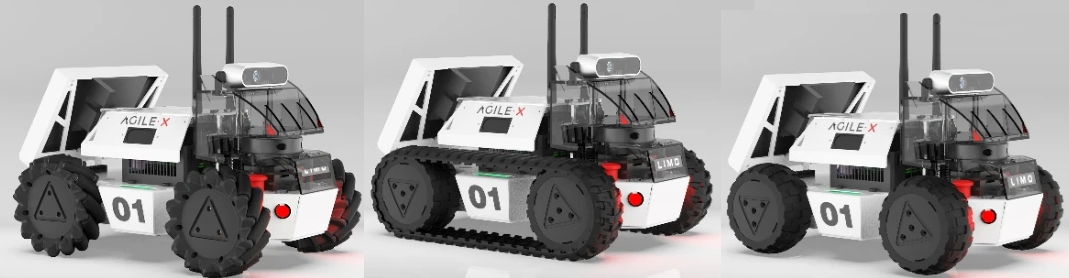
\includegraphics[trim=0 0 528 0, clip,  width=\textwidth]{img/Limo_modes.png}
        \caption{Robô Omnidirecional}
    \end{subfigure}
    ~
    \begin{subfigure}[b]{0.3\textwidth}
        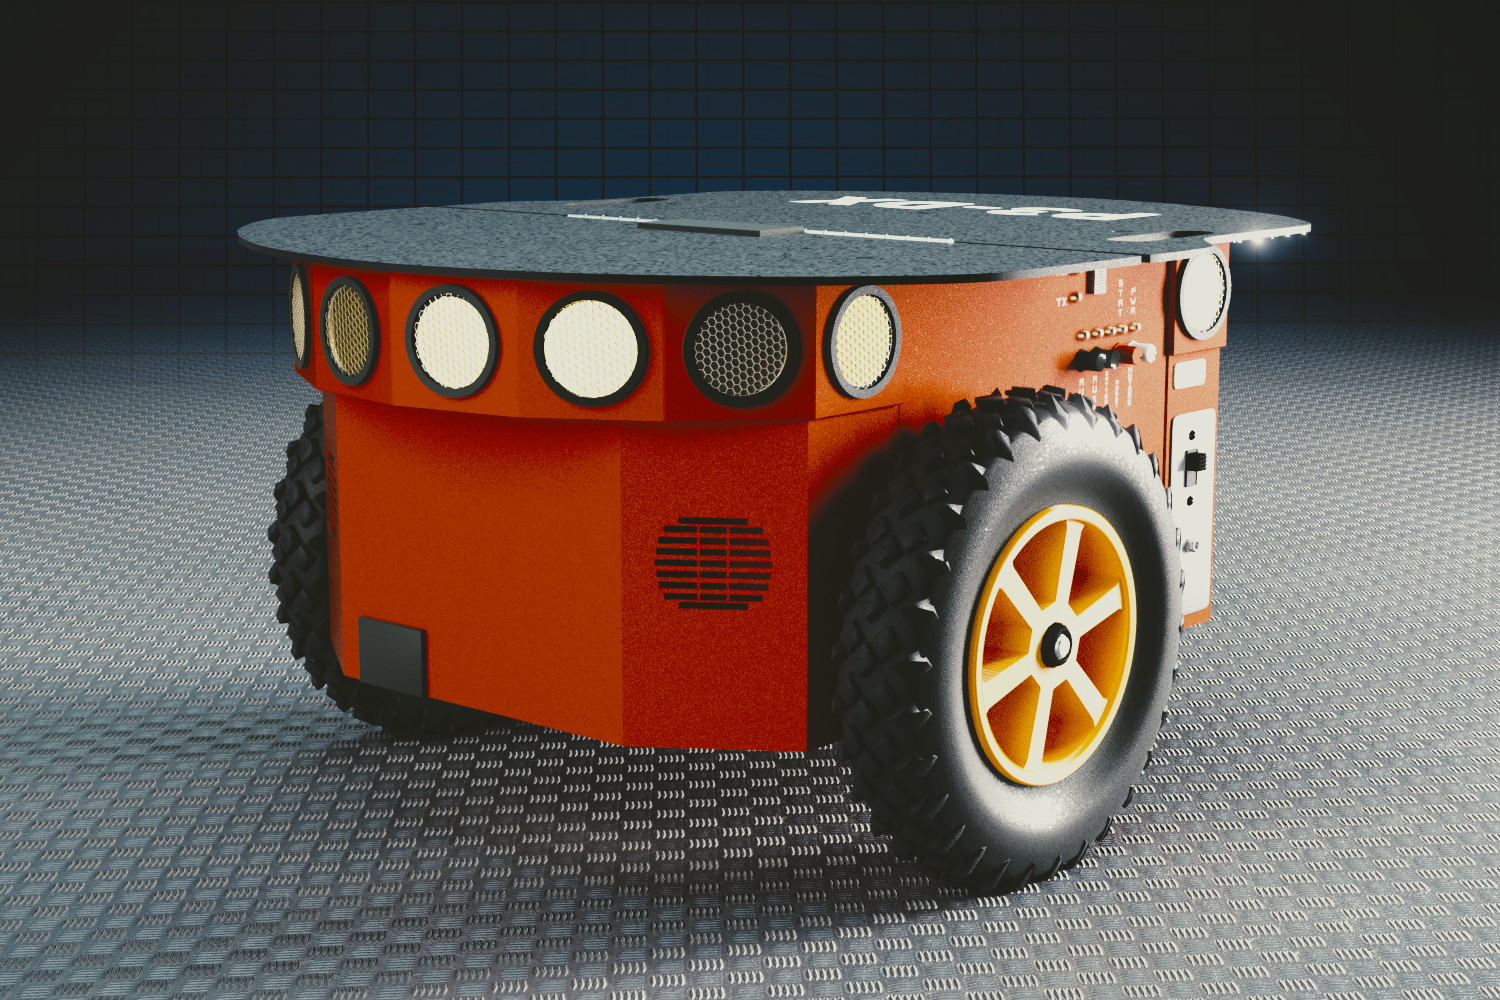
\includegraphics[width=\textwidth]{Pioneer 3-DX.jpg}
        \caption{Robô Diferencial Pioneer 3-DX}
    \end{subfigure}
    ~
    \begin{subfigure}[b]{0.3\textwidth}
        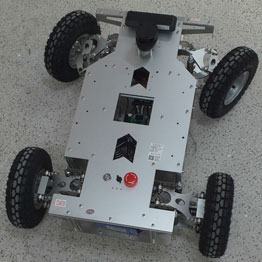
\includegraphics[width=\textwidth]{ackerman_robot.png}
        \caption{Robô Ackerman (\textit{car-like})}
    \end{subfigure}
    
    \sourceParbox[0.9\textwidth][\textbf{(a)} e \textbf{(c)}: \cite{Sarcinelli-Filho2023_2}; \textbf{(b)}: \cite{site:ArtStation_AynurZakirov}]
    % \source[\textbf{(a)} e \textbf{(c)}: \cite{Sarcinelli-Filho2023_2};\textbf{(b)} \cite{site:ArtStation_AynurZakirov}]
    % \note[0.8\linewidth][À esquerda, robô omnidirecional com rodas to tipo Mecanum e à direita robô diferencial (Uniciclo) Pioneer 3-DX]
\end{figure}


% >>> Comando para inserir a fonte em figuras <<<
% e.g.:
% \begin{figure}[!h]
%	\centering
%	\caption{Legenda da Figura.}
%	\includegraphics[width=0.7\textwidth]{figura.jpg}
%	\source[\citeonline{Referencia}.]
%	\label{fig:label_da_figura}
%  \end{figure}
%  
% Obs.: Se utilizar apenas "\source", será inserido
%       "Produção do próprio autor."

As plataformas móveis omnidirecionais são plataformas holonômicas (capazes de se mover em qualquer direção) e, portanto, não possuem restrições em seu sentido de movimento. Estas plataformas usam rodas projetadas especificamente para permitir movimentos nas direções transversais e longitudinais, permitindo que o robô obtenha velocidades em todas as direções do seu plano de trabalho (ver Figura \ref{fig:rodas_omnidirecionais}).

% incluir figura dos tipos de robos
\begin{figure}[htb]
    \caption{Rodas de Robôs Omnidirecionais}
    \centering    
    \begin{subfigure}[b]{0.2\textwidth}
        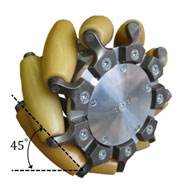
\includegraphics[width=\textwidth]{Omidirectional/omidirectional_robot_sarcinelli3.png}
        \caption{Roda Mecanum}
    \end{subfigure}
    \hspace{0.1\textwidth}
    \begin{subfigure}[b]{0.2\textwidth}
        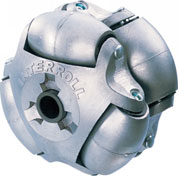
\includegraphics[width=\textwidth]{Omidirectional/omidirectional_robot_sarcinelli4.png}
        \caption{Roda \textit{Omni}}
    \end{subfigure}
    \source[Adaptado de \cite{Sarcinelli-FilhoControlRobots}]
    \label{fig:rodas_omnidirecionais}
\end{figure}


As plataformas móveis diferenciais são plataformas não holonômicas que contêm duas rodas principais, com motores independentes, responsáveis pelo movimento do robô. Geralmente, são equipadas com uma terceira roda, do tipo castor ou omnidirecional, para servir de apoio e manter o equilíbrio da plataforma.

Os robôs do tipo \textit{car-like} têm seu funcionamento semelhante ao dos carros utilizados no cotidiano, contando com uma plataforma com quatro rodas, duas localizadas na parte frontal e duas localizadas na parte traseira do \textit{chassis} do robô e apenas um motor é responsável pelo movimento, de modo que as duas rodas frontais são responsáveis pela direção do movimento, que ocorre ao rotacionar as rodas para a esquerda ou direita.

Nas próximas seções, discute-se o modelo cinemático de robôs diferenciais e os métodos de controle aplicáveis a esse tipo de robô, por se tratar do foco deste trabalho.


    \subsection{Modelo e Controle Cinemático de Robôs Diferenciais}
    \label{sec:Modelo_Robos_Diferenciais}
    
    Os robôs de tração diferencial são caracterizados por duas rodas de tração que podem girar em velocidades diferentes. Há também casos em que duas rodas do mesmo lado são acionadas por um único motor, alcançando uma configuração diferencial com quatro rodas. A Figura \ref{fig:Diff_Wheel} apresenta um esquema das velocidades do robô diferencial. Define-se, a princípio, o ponto central do eixo entre as rodas motorizadas do robô como o ponto de referência para a velocidade. Este será o ponto de controle, o ponto do robô que queremos controlar.

\begin{figure}[htb]
    \centering
    \caption{Velocidades características de um robô de tração diferencial, com o ponto de controle no ponto central do eixo das rodas.}
    \begin{subfigure}[b]{0.45\textwidth}
        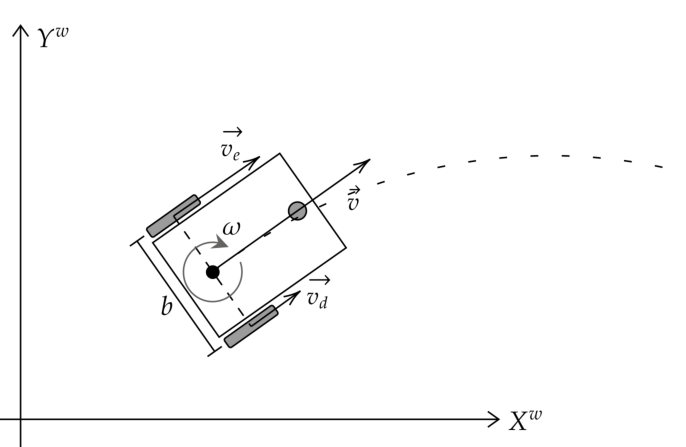
\includegraphics[trim=0 0 65 0, clip, width=\textwidth]{img/wheels_differential_speeds_crop.pdf}
        \caption{Esquema de velocidades do robô diferencial}
        \label{fig:Diff_Wheel_Velocities}
    \end{subfigure}
    \hspace{0.05\textwidth}
    \begin{subfigure}[b]{0.4\textwidth}
        \centering
        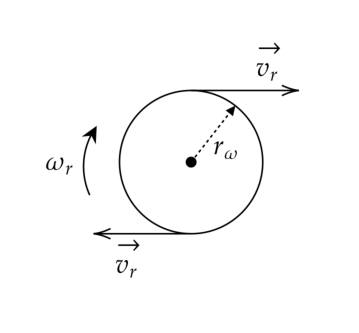
\includegraphics[width=0.7\textwidth]{img/wheel_speed_details_crop.pdf}
        \caption{Detalhe das velocidades das rodas do robô}
        \label{fig:Diff_Wheel_Detail}
    \end{subfigure}
    \source
    \label{fig:Diff_Wheel}
\end{figure}
    
    No ponto de controle definido, quando as rodas em lados opostos giram na mesma direção, o robô se move para frente com uma velocidade linear $(v)$. Se as rodas giram com velocidades de rotação diferentes, o robô desenvolve uma velocidade angular $(\omega)$. Essas velocidades podem ser expressas em termos das rotações das rodas esquerda $(\omega_e)$ e direita $(\omega_d)$ do robô.
    
    As velocidades linear $(v)$ e angular $(\omega)$  do ponto de controle podem ser obtidas pela média das velocidades exercidas por cada roda. Seja $\omega_E$ a velocidade angular do robô devido à roda esquerda e $\omega_D$ a velocidade angular devido à roda direita e definindo o sentido horário de movimento como positivo, teremos:

    \begin{eqnarray}
        v = \frac{v_e + v_d}{2} \qquad  \qquad \omega = \frac{\omega_E - \omega_D}{2}   \\
        v = \frac{v_e + v_d}{2} \qquad  \qquad \omega = \frac{\frac{v_e}{b/2} - \frac{v_d}{b/2}}{2}
    \end{eqnarray}
    
    % \begin{equation}
    %     v = \frac{v_e + v_d}{2}, \quad \omega = \frac{\frac{2v_e}{b} - \frac{2v_d}{b}}{2}
    % \end{equation}
    
    % \begin{equation}
    %     v = \frac{v_e + v_d}{2}, \quad \omega = (\frac{\cancel{2}v_e}{b} - \frac{\cancel{2}v_d}{b})\cdot\frac{1}{\cancel{2}}
    % \end{equation}

    Simplificando, obtemos:

    \begin{equation}
        v = \frac{v_e + v_d}{2} \qquad \text{e} \qquad \omega = \frac{v_e-v_d}{b}
    \end{equation}
    
    e com base na Figura \ref{fig:Diff_Wheel_Detail}, obtém-se as velocidades do robô em função das rotações das rodas esquerda e direita como:
    
    \begin{equation} 
    v = \frac{(\omega_e + \omega_d)r_w}{2} \qquad \text{e} \qquad \omega = \frac{(\omega_e - \omega_d)r_w}{b}, 
    \end{equation} 
    
    onde $r_w$ é o raio da roda e $b$ é a distância entre as rodas de um lado e as do outro \cite{Bouzoualegh2018ModelRobot} \cite{book:siegwart2011} \cite{Sarcinelli-Filho2023KinematicModels}.

    Para controlar as rotações das rodas esquerda e direita, sinais PWM são enviados para os controladores eletrônicos de velocidade (ESCs) montados em cada um dos motores. No entanto, a maioria dos robôs móveis podem ser controlados por sinais de controle de alto nível (comandos de velocidade linear e angular), a saber $ \bs{u} = \begin{bmatrix} v & \omega \end{bmatrix}^T $. Isso é possível pois os fabricantes implementam o controlador de baixo nível a bordo do veículo, que gera os sinais de controle PWM para mover as rodas a partir das velocidades de entrada e do modelo da dinâmica do veículo. Isso permite o controle das velocidades linear e angular do veículo usando sinais de controle de alto nível, com perda de desempenho mínima para movimentos de baixa aceleração. Portanto, para controlar o robô diferencial somente é necessário definir os comandos de velocidades linear e angular que este deve executar.

    % Para definir o controlador cinemático, utilizaremos o modelo de cinemática extendida do robô diferencial, pois este modelo permite o controle de qualquer ponto...
    O controlador utilizado neste trabalho é obtido pela técnica de cinemática inversa \cite{Sarcinelli-Filho2023_4}. Para utilizá-la, é necessário obter o modelo cinemático de um robô diferencial terrestre de modo que o ponto de controle não tenha restrições holonômicas e possa desenvolver velocidades nos dois eixos de referência do robô ($X^r$ e $Y^r$) \cite{Sarcinelli-Filho2023_2}. Com base na Figura \ref{fig:differential_mode}, podemos obter este modelo a partir das relações trigonométricas entre o referencial inercial do mundo e o referencial do robô, utilizando como ponto de controle o ponto $\bs{x}_c$, deslocado longitudinalmente do ponto $\bs{x}$.
    
    \begin{figure}[htb]
        \centering
        \caption{Cinemática 2D de um robô diferencial, mostrando a parte frontal do robô. A posição do robô, $ \bs{x} $, é deslocada por um valor \( a \). Isso resulta em um novo vetor de posição \( \bs{x}_c \), uma mudança que simplifica a implementação do controlador cinemático.}
        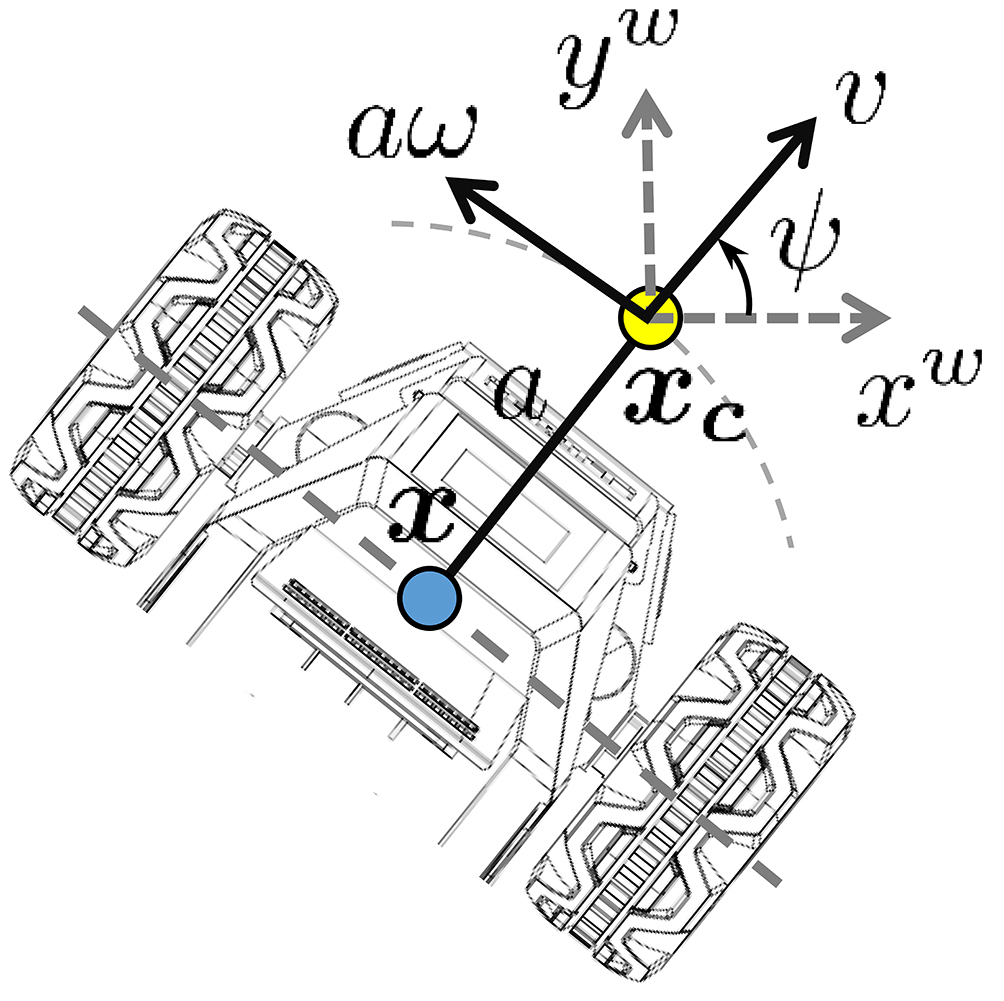
\includegraphics[width=0.4\linewidth]{limo_diff.jpg} 
        \label{fig:differential_mode}
        \source
    \end{figure}
    
    As relações entre as velocidades $v$ e $w$ do robô e as velocidades correspondentes no eixo inercial do mundo serão:
    
    \begin{align}
        \dot{x}_c &= v\cos{\psi} - a\omega\sin{\psi}   \\
        \dot{y}_c &= v\sin{\psi} + a\omega\cos{\psi}    \\
        \dot{\psi} &= \omega
    \end{align}

    que em notação matricial, fica:

    \begin{equation}
        \begin{bmatrix} \dot{x}_c \\ \dot{y}_c  \end{bmatrix} = \begin{bmatrix} \cos{\psi} & -a \sin{\psi} \\ \sin{\psi} & a \cos{\psi}   \end{bmatrix} \cdot \begin{bmatrix} v \\ \omega    \end{bmatrix}
        \label{eq:kinematics_differential}
    \end{equation}
    
    ou seja, \( \dot{\bs{x}}_c = \bs{H} \bs{u} \), em que $\bs{H}$ é a matriz de cinemática do robô diferencial \cite{Sarcinelli-Filho2023_2}. Note que esta matriz é invertível, o que permite obter a equação para o controlador utilizando a técnica de cinemática inversa \cite{Sarcinelli-Filho2023_4}, de tal forma que $\bs{u} = \bs{H}^{-1} \dot{\bs{x}}_{c,ref}$, ou, 
    
    \begin{align}
        \label{eq:kinematic_controller_differential}
        \dot{\bs{u}} \ \  & = \qquad \;  \bs{H}^{-1} \quad\;\; \cdot \; \; \bs{x}_{c\,ref}    \notag \\
        \begin{bmatrix} v \\ \omega    \end{bmatrix} & =  \begin{bmatrix} c_\psi & s_\psi \\ -\frac{1}{a}s_\psi & \frac{1}{a} c_\psi   \end{bmatrix} \cdot \begin{bmatrix}\dot{x}_{c,ref} \\ \dot{y}_{c,ref}   \end{bmatrix}
    \end{align}
    
   onde $ c(\cdot) $ e $ s(\cdot) $ representam as funções $ cosseno() $ e $ seno() $, respectivamente.
    
    A velocidade de referência \( \dot{\bs{x}}_{c,ref} \) é uma lei de controle de \textit{feedforward} e \textit{feedback} proporcional, tal que
    
    \begin{equation}
        \dot{\bs{x}}_{c,ref} = \dot{\bs{x}}_{c,des} + \bs{\kappa}(\bs{x}_{c,des} - \bs{x}_c),
        \label{eq:ff_fb_law}
    \end{equation}
    
    \noindent para o qual \( \bs{\kappa} \) é a matriz de ganhos do controlador, que deve ser uma matriz diagonal definida positiva.

    % \subsection{Controle de Robôs Diferenciais}
    % \label{sec:Controle_Robos_Diferenciais}

    
% \begin{itemize} 
%     \item \add{Controle de Posicionamento}
%     \item \add{Seguimento de Trajetória}
% \end{itemize}    

\section{Localização e Mapeamento Simultâneos}

No contexto da robótica móvel, o problema de Localização e Mapeamento Simultâneos (SLAM, do inglês \textit{Simultaneous Localization and Mapping}) surge como um dos desafios fundamentais para a autonomia de robôs. Em essência, o robô precisa construir um mapa de um ambiente desconhecido ao mesmo tempo em que estima sua própria pose (posição e orientação) dentro desse mapa \cite{Thrun2005}. Trata-se de uma tarefa complexa pois, diferentemente da simples localização com mapa previamente conhecido ou do mapeamento com pose conhecida, no SLAM tanto o mapa quanto a pose são inicialmente desconhecidos e precisam ser estimados\cite{Thrun2005}. 

Nas últimas décadas, pesquisas em SLAM alcançaram progressos notáveis, viabilizando aplicações em larga escala e até sua transição para setores industriais \cite{Yue2024} \cite{Cadena2016}. Ainda assim, o SLAM permanece um problema em aberto em muitos aspectos, especialmente devido a seus principais desafios práticos: a presença de incertezas significativas nas medições sensoriais e nos movimentos do robô, a necessidade de identificar fechamentos de ciclo de forma confiável, e a correta associação de dados sensoriais a elementos do mapa \cite{Yue2024} \cite{Placed2023AFrontiers} \cite{Bavle2023FromSurvey}.

A incerteza inerente aos sensores e à odometria faz com que erros se acumulem ao longo do deslocamento do robô, exigindo técnicas robustas para manter a estimativa consistente. Para isso, é necessário a detecção de fechamentos de ciclo (\textit{loop closure}), que consiste em detectar quando o robô retorna a uma região já mapeada – crucial para corrigir desvios acumulados no mapa e na pose \cite{Labbe2014}, o que depende de técnicas de associação de dados a fim de determinar quais observações correspondem a quais características do mapa (ou a novos marcos), evitando correspondências equivocadas que poderiam degradar o mapa \cite{Cadena2016}.

Diversos algoritmos foram propostos para tentar solucionar o problema de SLAM, combinando conceitos de robótica probabilística e otimização \cite{Thrun2005}\cite{Cadena2016}. A seguir são apresentados os principais tipos de algoritmos de SLAM, com uma breve descrição de cada um e suas características.

    \subsection{Tipos de Algoritmos de SLAM}
    
    Ao longo do desenvolvimento do SLAM, diferentes abordagens baseadas em estimadores Bayesianos e em técnicas de otimização foram exploradas. Entre os tipos mais influentes estão algoritmos baseados em filtro de Kalman estendido(EKF, do inglês \textit{Extended Kalman Filter}), em filtros de partículas e em grafos de otimização. Cada categoria apresenta formas distintas de representar e estimar o mapa e a pose do robô, com vantagens e limitações específicas, conforme descrito a seguir.
    
        \subsubsection{EKF-SLAM}
        
        Uma das abordagens clássicas para o SLAM é o \textbf{EKF-SLAM}, que emprega um Filtro de Kalman Estendido para estimar iterativamente o estado do robô e do mapa \cite{Thrun2005}. Nessa formulação, o estado mantido pelo filtro inclui a pose atual do robô e as posições estimadas de todos os marcos (landmarks) mapeados no ambiente. 
        
        O EKF propaga uma distribuição Gaussiana conjunta sobre este vetor de estado, atualizando um grande vetor de média e uma matriz de covariância a cada movimento executado (etapa de previsão) e a cada nova observação sensorial (etapa de correção) \cite{Thrun2005}. Intuitivamente, o EKF-SLAM começa sem nenhum marco conhecido; conforme o robô explora o ambiente e detecta novos marcos, estes são adicionados ao estado, e tanto a localização do robô quanto as posições dos marcos são refinadas. O filtro lineariza as funções não-lineares de movimento e percepção em torno do estado estimado (base do EKF), permitindo calcular a atualização de forma analítica, porém aproximada \cite{Thrun2005}. 
        
        A principal vantagem dessa abordagem é fornecer diretamente uma estimativa estatística completa (média e incerteza) tanto da pose quanto do mapa, capturando as correlações entre todas as variáveis. Isso permite, por exemplo, que o robô avalie quantitativamente sua incerteza de localização ao decidir seus próximos movimentos, tornando o sistema mais consciente de suas limitações. Entretanto, o EKF-SLAM apresenta alto custo computacional: a cada passo de atualização, a complexidade tende a crescer quadraticamente com o número de marcos mapeados, pois a matriz de covariância cresce com o quadrado do número de variáveis (pose + marcos), tornando a atualização cada vez mais custosa à medida que o mapa cresce. \cite{Thrun2005}. Isso restringe a escalabilidade para mapas grandes ou muito detalhados. Além disso, o método assume erros gaussianos e pequenas não-linearidades; em cenários de forte não-linearidade ou ambientes com marcos muito similares (causando ambiguidades), o EKF pode produzir estimativas inconsistentes ou até divergir \cite{Thrun2005}. A associação de dados, em particular, torna-se crítica: o EKF-SLAM geralmente utiliza a correspondência de máxima verossimilhança incremental para parear observações com marcos existentes, o que impede a revisão de associações passadas \cite{Thrun2005}. Uma má associação de dados (por exemplo, confundir dois marcos semelhantes) propaga erro sem possibilidade de revisão posterior, diferente de métodos baseados em grafos, como Graph-SLAM, que permitem reotimizar o mapa a posteriori. 

% \begin{algorithm}[H]
%     \caption{Algoritmo genérico para o EKF-SLAM}
%     \alg
%     \SetAlgoLined
%     \FuncSty{EKF\_SLAM(}\ArgSty{pose_anterior}) \
%         initialization\;
%     \While{not at end of this document}{
%         read current\;
%     \eIf{understand}{
%         go to next section\;
%         current section becomes this one\;
%     }{
%         go back to the beginning of current section\;
%     }
%     \If{$\Delta$ == true}{
%         show the match}
%     }

% \end{algorithm} 
        
        \subsubsection{FastSLAM – SLAM usando Filtro de Partículas}
        
        Para contornar algumas das limitações do EKF-SLAM, foi introduzido o \textit{FastSLAM}, uma família de algoritmos que aplicam filtros de partículas ao problema de SLAM \cite{Montemerlo2002} \cite{Thrun2005}. O FastSLAM explora a técnica de fatoração do problema de SLAM através de um filtro de partículas Rao-Blackwellizado. A ideia central é separar (matematicamente, fatorar) a estimativa da trajetória do robô da estimativa do mapa, aproveitando a independência condicional dos marcos (\textit{Landmarks}) quando a trajetória do robô é conhecida \cite{Montemerlo2002}. Em prática, o algoritmo mantém um conjunto de partículas, onde cada partícula representa uma hipótese para a trajetória percorrida pelo robô (sequência de poses estimadas) e possui seu próprio mapa associado (estimativas dos marcos) \cite{Thrun2005}. Dentro de cada partícula, as posições dos marcos são estimadas de forma local, tipicamente usando pequenos filtros de Kalman individuais para cada marco. Dessa forma, o filtro de partículas lida com a incerteza global da trajetória, enquanto os filtros locais (um por marco) lidam com a incerteza das posições dos marcos dada a trajetória conhecida. Essa abordagem fatorada reduz drasticamente a necessidade de manter e atualizar uma grande matriz de covariância conjunta, o que melhora a escalabilidade: a complexidade de atualização cresce linearmente com o número de marcos (multiplicado pelo número de partículas), em vez de quadraticamente \cite{Thrun2005}. Em muitas aplicações, um conjunto relativamente pequeno de partículas (dezenas a centenas) é suficiente para obter bons resultados, tornando o FastSLAM capaz de mapear ambientes maiores sem explosão do custo computacional. 
        
        O algoritmo FastSLAM original (às vezes chamado de FastSLAM 1.0) foi apresentado por Montemerlo et al. (2002) utilizando amostragem de partículas conforme a distribuição de movimento do robô, e posteriormente aprimorado no FastSLAM 2.0 com técnicas de amostragem mais informativas para melhorar a precisão \cite{Montemerlo2002}. Uma das grandes vantagens do FastSLAM é sua robustez em cenários onde o EKF-SLAM enfrentaria problemas de não-linearidade ou multi-modalidade na distribuição de probabilidade: o conjunto de partículas pode, teoricamente, representar hipóteses múltiplas sobre a pose do robô (por exemplo, diferentes posicionamentos caso o robô se localize em locais parecidos), coisa que um único filtro gaussiano não consegue fazer. Além disso, o FastSLAM permite incorporar facilmente observações com associações de dados diferentes em partículas distintas – ou seja, diferentes partículas podem “apostar” em associações de dados alternativas, mitigando em parte o risco de um erro de correspondência arruinar todo o mapa \cite{Thrun2005}. Entretanto, o FastSLAM também tem desvantagens. Uma delas é que, apesar de não manter explicitamente uma matriz de covariância completa, ele pode degradar em performance se o número de partículas necessário for alto – por exemplo, em ambientes muito extensos ou após longos percursos sem fechamento de ciclo, pode ser preciso um grande número de partículas para manter a consistência, o que aumenta o custo computacional e de memória. Outro ponto é que o erro de trajetória do robô (contido nas partículas) pode crescer ao longo do tempo; se poucas partículas sobreviverem representando corretamente a distribuição verdadeira da pose, o filtro de partículas pode sofrer de degeneração (perda de diversidade), tornando difícil recuperar um fechamento de ciclo tardio caso as partículas restantes não estejam próximas da solução correta \cite{Thrun2005}. Em outras palavras, o FastSLAM tende a tratar as correlações entre marcos de forma implícita via as partículas e, se essa representação implícita for insuficiente, podem ocorrer inconsistências, especialmente no momento de grandes fechamentos de loop \cite{Thrun2005}. Ainda assim, na prática, o FastSLAM mostrou-se muito eficaz e foi durante um período a técnica de estado da arte, sendo capaz de mapear trajetórias de quilômetros com precisão comparável a dos métodos de filtro gaussiano tradicionais, porém com melhor escalabilidade \cite{Thrun2005}. Esse método abriu caminho para SLAM em tempo real com veículos autônomos e robôs de serviço em ambientes maiores, e influenciou também algoritmos modernos de mapeamento baseados em grades de ocupação (ocupancy grids) e SLAM visual que empregam partículas ou múltiplas hipóteses \cite{Thrun2005}.

        
        \subsubsection{SLAM Baseado em Grafos}
        
        Nos últimos anos, a abordagem dominante para SLAM tem se voltado aos métodos baseados em grafos, também conhecidos como \textit{Graph-Based SLAM} ou \textit{GraphSLAM} \cite{Grisetti2010}\cite{Labbe2014}. Diferentemente das abordagens discutidas anteriormente, que utilizam filtros sequenciais (a estimativa de pose atual é dependente das estimativas anteriores), o SLAM baseado em grafos formula o problema como uma otimização global: constrói-se um grafo de variáveis que representa o histórico de poses do robô (cada nó no grafo é uma pose do robô em um determinado instante, ou alternativamente, um marco mapeado, dependendo da formulação) e as medições são representadas por arestas que conectam os nós, impondo restrições espaciais entre poses (ou entre pose e marco) \cite{Labbe2014}. Por exemplo, a odometria do robô introduz arestas conectando cada pose com a pose seguinte, enquanto uma observação de um marco visto em duas poses diferentes gera uma aresta de restrição entre essas poses (ou entre pose e nó de marco). O objetivo então é encontrar os valores de todas as poses (e eventualmente das coordenadas dos marcos) que melhor satisfazem todas as restrições do grafo – tipicamente formulado como um problema de mínimos quadrados não-lineares, resolvido por métodos de otimização iterativa (como Gauss-Newton, Levenberg-Marquardt, etc.) \cite{Zhang2021}. Em essência, o Graph-SLAM procura a configuração de mapa e trajetória com máxima consistência global, em vez de atualizar as estimativas de pose incrementalmente a cada iteração do algoritmo.
        
        A vantagem clara dessa formulação é que ela lida de forma natural com o fechamento de ciclo e com múltiplas restrições redundantes. Quando o robô detecta um lugar previamente visitado (loop closure), adiciona-se uma nova aresta no grafo conectando as poses correspondentes; a otimização do grafo então ajusta todas as poses de maneira coerente para acomodar essa nova informação, distribuindo o erro acumulado pelo laço fechado \cite{Labbe2014}. Diferentemente do EKF, que propagava correlações de maneira implícita e incremental, o grafo torna explícitas as relações entre poses e permite recalcular o mapa inteiro de forma consistente ao encontrar novas relações. Além disso, a estrutura esparsa do problema (cada medida relaciona apenas algumas variáveis) pode ser explorada para eficiência: técnicas de otimização de grafos conseguem resolver mapas com milhares de poses e restrições em tempo real ou próximo de tempo real, algo impraticável para um EKF que manteria um gigantesco vetor de estado denso \cite{Grisetti2010}. Na literatura, diversos frameworks de otimização de grafos foram desenvolvidos para SLAM, como por exemplo \textit{iSAM}, \textit{g2o}, entre outros, que aplicam estratégias de linearização incremental e fatoração matricial aproveitando a esparsidade das jacobianas \cite{Juric2021ASLAM} \cite{Kummerle2017G2o:Optimization} \cite{Kaess2008ISAM:Mapping} \cite{Li2021Gumbel-softmax-basedGraphs}. Como resultado, o SLAM baseado em grafos tornou-se a espinha dorsal de muitos sistemas modernos de mapeamento. Por exemplo, algoritmos de SLAM visual de última geração tipicamente mantêm um grafo de poses de câmera (frequentemente chamadas de keyframes) e realizam otimizações globais conhecidas como \textit{bundle adjustment} ou otimização de \textit{pose graph} para minimizar a reprojeção de pontos no mapa \cite{MurArtal2017}\cite{Zhang2021}. No caso de SLAM com sensores RGB-D ou LiDAR, também é comum construir um grafo de poses onde cada aresta representa a correspondência entre nuvens de pontos ou características visuais detectadas entre duas poses, e então um otimizador distribui os erros ao longo do grafo \cite{Zhang2021}. 
        
        Um ponto importante do SLAM por grafo é a separação conceitual entre o \textit{front-end} e o \textit{back-end} do sistema. O \textit{front-end} é responsável por processar os dados brutos dos sensores para extrair informações relevantes (por exemplo, detectar feições visuais ou geometrias em um laser) e por tomar decisões de associação de dados e detecção de fechamentos de loop – ou seja, construir as arestas do grafo de forma correta. Já o \textit{back-end} pega esse grafo de restrições construído e realiza a otimização matemática para ajustar as estimativas de pose/mapa \cite{Cadena2016}. Essa modularidade permite incorporar técnicas avançadas de reconhecimento de lugares (como detecção de loop closures baseada em visão, descritores de imagem, etc) sem modificar o núcleo do estimador, e vice-versa, possibilitando aplicar algoritmos de otimização genéricos independentemente do tipo de sensor utilizado \cite{Labbe2014}. Entretanto, o desempenho do Graph-SLAM depende criticamente da qualidade do front-end: associações de dados incorretas podem degradar a solução se não forem tratadas, exigindo esquemas robustos para rejeitar \textit{outliers} ou usar funções de perda robusta na otimização. Ainda assim, a abordagem de grafo é atualmente considerada o estado da arte em SLAM devido à sua precisão e flexibilidade. Estudos e sistemas recentes confirmam sua eficácia em cenários reais complexos, incluindo mapeamento de longo prazo e multi-sessão \cite{Labbe2014}, SLAM visual e RGB-D em larga escala \cite{MurArtal2017} \cite{Zhang2021}, entre outros.

        Como demonstrado por \citeonline{Labbe2014}, a detecção confiável de fechamentos de ciclo em um SLAM gráfico de larga escala pode lidar até com cenários de mapeamento multi-sessão, nos quais o robô pode ser reinicializado em locais diferentes e ainda assim unificar os mapas através de correspondências encontradas posteriormente. Assim, o SLAM baseado em grafos oferece uma solução elegante e eficaz para o problema de localização e mapeamento simultâneos, motivo pelo qual foi adotado neste projeto.
        
        Vale destacar que o presente trabalho utiliza um método de SLAM baseado em grafos, a \textbf{SLAM Toolbox} \cite{site:Slam_toolbox}. Optou-se pela utilização desta biblioteca de SLAM robusta e amplamente testada, presente no ecossistema ROS (Robot Operating System). A utilização desta biblioteca é recomendada nos tutoriais de SLAM do pacote Nav2 do ROS 2, o pacote padrão utilizado para navegação de robôs, demonstrando a confiança da comunidade ROS nesta biblioteca. 

%%%%%%%%%%%%%%%%%%%%%%%%%%%%%%%%%%%%%%%%%%%%%%%%%%%%%
%%%%%%%%%%%%%%%%%%%%%%%%%%%%%%%%%%%%%%%%%%%%%%%%%%%%%
%%%%%%%%%%%%%%%%%%%%%%%%%%%%%%%%%%%%%%%%%%%%%%%%%%%%%

\ifisTipoDocumento
    % PG
    \chapter[Metodologia e etapas de desenvolvimento]{Metodologia e etapas de desenvolvimento}
    
    \section{Metodologia Adotada}


\txr{DICA:} Antes de escrever está seção recomendo ler o Anexo \ref{sec:TrainDeepModel}.


O trabalho será desenvolvido conforme as etapas apresentadas a seguir.

\begin{itemize}
\item 
\textbf{Etapa 1.} Estudo teórico:
(\textit{i}) estudo sobre xxxx;
(\textit{ii}) revisão a respeito de xxxx.
\item 
\textbf{Etapa 2.} Especificações do projeto:
(\textit{i}) dimensionar as xxxx;
(\textit{ii}) definir o xxxxx;
\item 
\textbf{Etapa 3.} Desenvolvimento do sistema:
(\textit{i}) realizar as xxxx;
(\textit{ii}) desenvolver o xxxx.
\item 
\textbf{Etapa 4.} Teste do sistema:
(\textit{i}) realizar xxxx;
(\textit{i}) fazer xxxx;
\item 
\textbf{Etapa 5.} Documentação:
(\textit{i}) Documentar o projeto de graduação.
\end{itemize}

\section{Cronograma de Trabalho}

\txr{DICA:} O seguinte é um \textit{template} de \href{https://pt.wikipedia.org/wiki/Diagrama_de_Gantt}{Diagrama de Gantt} para \LaTeX. Para entender a organização do \textit{template} é necessário compreender que faz o comando \verb|\newcommand{\name_comand}{value}|: resumidamente, ele permite criar o comando  \verb|\name_comand|, tal que, cada vez que usamos no escrito o comando \verb|\name_comand| seu valor representado pela \textit{string} \verb|value| é incluído no texto. Então, a logica do \textit{template} é a seguinte: 
(1) definimos na variável \verb|\DuracionPlanoMeses| o número de meses usados para a implementação do projeto; 
(2) definimos como comandos as atividades a ser feitas; 
(3) definimos como comandos os rótulos relacionados com cada atividade, tal que, os referidos rótulos são usados no diagrama de Gantt; 
(4) escrevemos alguns comentários sobre o diagrama de atividades;
(5) Criamos a tabela de atividades, aqui são usados os comandos definidos no passo (2);
(6) Criamos o Diagrama de Gantt das Atividades, aqui são usados os comandos dos rótulos definidos no passo (3). 

%1. DEFINIMOS O NUMERO DE MESES NOS QUAIS SERÁ IMPLEMENTADO O PROJETO
\newcommand{\DuracionPlanoMeses}{8}

%2. DEFINIMOS AS ATIVIDADES COMO COMANDOS VIA \newcommand{\name_comand}{value}
%primeira atividade
\newcommand{\AtvAlgRotI}{Estudo sobre xxx e revisão sobre xxxx.}
%segunda atividade
\newcommand{\AtvAlgRotII}{Dimensionar as xxxx e definir yyyy}
%terceira atividade
\newcommand{\AtvAlgRotIII}{realiar as xxx e desenvolver yyy.}
%quarta atividade
\newcommand{\AtvAlgRotIV}{Construir xxx.}
%quinta atividade
\newcommand{\AtvAlgRotV}{Treinar xxx.}
%quinta atividade
\newcommand{\AtvAlgRotVI}{Testar xxx.}
%quinta atividade
\newcommand{\AtvAlgRotVII}{Escrever o TCC.}

%3. DEFINIMOS OS ROTULOS DAS AS ATIVIDADES A SER USADAS NO DIAGRAMA DE GANTT USANDO O COMANDO \newcommand{\name_comand}{value}
%ROTULOS DE ATIVIDADES
\newcommand{\RTLAtvAlgRotI}{ETAP 1} %rotulo da primeira atividade
\newcommand{\RTLAtvAlgRotII}{ATV 2} %rotulo da segunda atividade
\newcommand{\RTLAtvAlgRotIII}{ATV 3} %rotulo da terceira atividade
\newcommand{\RTLAtvAlgRotIV}{ATV 4} %rotulo da quarta atividade
\newcommand{\RTLAtvAlgRotV}{ATV 5} %rotulo da quinta atividade
\newcommand{\RTLAtvAlgRotVI}{ATV 6} %rotulo da sexta atividade
\newcommand{\RTLAtvAlgRotVII}{ATV 7} %rotulo da sétima atividade

%4. COMENTARIOS SOBRE O DIAGRAMA DE ATIVIDADES
Apresenta-se nesta seção uma previsão do cronograma do plano de trabalho. O tempo total deste é de \DuracionPlanoMeses\ meses.

Na Tabela \ref{Tab1}, são detalhadas as atividades que se pretendem realizar para o desenvolvimento do plano de trabalho. 
Assim na primeira coluna da tabela são definidos os rótulos de cada atividade e na segunda coluna é feita uma descrição da atividade que se pretende realizar. Finalmente na Figura \ref{figDAGRTEMPACT001} é apresentado o diagrama de tempos das atividades indicadas na Tabela \ref{Tab1}.

%5. CRIAÇÃO DA TABELA DE ATIVIDADES, OBSERVE QUE AQUI SÃO USADOS OS COMANDOS DAS ATIVIDADES
\begin{table}[!htbp]
\begin{center}\begin{tabular}{c|p{14.00cm}}
\hline
Rótulo  & Atividade \\ 
\hline
\hline
\RTLAtvAlgRotI & \AtvAlgRotI \\ 
\hline 
\RTLAtvAlgRotII & \AtvAlgRotII \\ 
\hline 
\RTLAtvAlgRotIII & \AtvAlgRotIII \\ 
\hline
\RTLAtvAlgRotIV & \AtvAlgRotIV \\ 
\hline
\RTLAtvAlgRotV & \AtvAlgRotV \\
\hline
\RTLAtvAlgRotVI & \AtvAlgRotVI \\
\hline
\hline
\RTLAtvAlgRotVII & \AtvAlgRotVII \\
\hline 
\end{tabular}
\end{center}
\caption{
\footnotesize
Lista de atividades. 
}
\label{Tab1}
\end{table}

%6. CRIAÇÃO DO DIAGRAMA DE GANTT DAS ATIVIDADES, OBSERVE QUE AQUI SÃO USADOS OS COMANDOS DOS  ROTULOS DAS ATIVIDADES
\begin{figure}[!htbp]
\begin{center}
\begin{ganttchart}[
x unit = 0.8cm,
y unit title=0.5cm,
y unit chart=0.5cm,
hgrid,vgrid,
title label anchor/.style={below=-1.6ex},
title height=1,
bar/.style={fill=gray!50},
%group/.style={draw=black},
incomplete/.style={fill=white},
progress label text={},
bar height=0.7,
%group right shift=0,
group top shift=.6,
group height=.3,
group peaks width=.2]{1}{12}
%labels
\gantttitle{2014}{12}\\
\gantttitle{\tiny JAN}{1} 
\gantttitle{\tiny FEV}{1} 
\gantttitle{\tiny MAR}{1} 
\gantttitle{\tiny ABR}{1} 
\gantttitle{\tiny MIO}{1} 
\gantttitle{\tiny JUN}{1} 
\gantttitle{\tiny JUL}{1}
\gantttitle{\tiny AGO}{1} 
\gantttitle{\tiny SET}{1} 
\gantttitle{\tiny OUT}{1} 
\gantttitle{\tiny NOV}{1} 
\gantttitle{\tiny DEZ}{1}\\
%tasks
% Tercceira técnica
\ganttbar[bar/.style={fill=blue},bar label font=\color{blue}]{\RTLAtvAlgRotI}{1}{2} \\
\ganttbar[bar/.style={fill=blue},bar label font=\color{blue}]{\RTLAtvAlgRotII}{3}{4} \\
\ganttbar[bar/.style={fill=blue},bar label font=\color{blue}]{\RTLAtvAlgRotIII}{5}{6} \\
\ganttbar[bar/.style={fill=blue},bar label font=\color{blue}]{\RTLAtvAlgRotIV}{7}{8} \\
\ganttbar[bar/.style={fill=blue},bar label font=\color{blue}]{\RTLAtvAlgRotV}{9}{10} \\
\ganttbar[bar/.style={fill=blue},bar label font=\color{blue}]{\RTLAtvAlgRotVI}{11}{12} \\
\ganttbar[bar/.style={fill=green},bar label font=\color{green}]{\RTLAtvAlgRotVII}{3}{11}
\end{ganttchart}
\end{center}
\caption{Diagrama de tempos das atividades a efetuar para o desenvolvimento do plano de trabalho. }
\label{figDAGRTEMPACT001}
\end{figure}
\else
    % TCC
    \chapter[Metodologia]{Metodologia}
    
% \begin{itemize}
%     \item \add{Descrição do ambiente experimental e das plataformas utilizadas (robôs, sensores, sistema OptiTrack e a plataforma LIMO, se aplicável).}
%     \item \add{Apresentação do SLAM\_toolbox: principais funcionalidades, justificativa para a escolha e forma de integração com o sistema de robôs.}
%     \item \add{Detalhamento da metodologia de comparação: critérios, métricas de desempenho (erro de localização, tempo de processamento, robustez, etc.) e a forma de coleta e análise dos dados.}
% \end{itemize}

% \add{Neste capítulo deverão ser descritos os recursos usados para a realização do projeto (equipamentos, material bibliográfico, programas de simulação, etc.), bem como aspectos relativos à disponibilidade ou não dos mesmos para a realização do estudo. Caso a disponibilidade de algum recurso seja limitada, ou esteja vinculada a alguma data de entrega, fator externo ou, até mesmo, a outro projeto, tal informação deve ser apresentada de forma explícita e clara nesta seção. O atraso ou a indisponibilidade deste recurso afetará diretamente o cronograma de execução do projeto, fato que deve ser cuidadosamente avaliado na construção do cronograma.}

\label{Cap03:Metodologia}
%% ----------------------------------------------
%%
%% -                  RECURSOS                  -
%%
%% ----------------------------------------------
Este trabalho se propôs a explorar algoritmos de localização, mapeamento e planejamento de rotas utilizando robôs móveis. Inicialmente, a proposta era desenvolver algoritmos próprios de SLAM para criação de mapas e localização no ambiente do laboratório, mas as dificuldades técnicas e restrições de tempo levaram à escolha de uma abordagem mais robusta. Assim, optou-se pela utilização da \textit{SLAM Toolbox}\cite{site:Slam_toolbox}, uma biblioteca de SLAM robusta e amplamente testada, presente no ecossistema ROS (Robot Operating System). A utilização desta biblioteca é recomendada nos tutoriais de SLAM do pacote Nav2 do ROS 2, o pacote padrão utilizado para navegação de robôs, demonstrando a confiança da comunidade ROS nesta biblioteca.

Assim, este projeto se propõe a utilizar a SLAM Toolbox para localização e mapeamento de robôs móveis terrestres no ambiente do LAB-AIR e analisar a qualidade do posicionamento e do controle utilizado para os robôs desenvolverem trajetórias definidas, usando o sistema de câmeras OptiTrack presente no laboratório como referência de alta precisão (\textit{ground-truth}).

Para isso, utilizou-se da estrutura pré-existente do Laboratório de Automação Inteligente e Robótica (LAB-AIR), que dispõe de robôs móveis terrestres e aéreosalém de um sistema de câmeras OptiTrack empregado como referência de alta precisão (\textit{ground-truth}) na verificação do desempenho dos algoritmos de localização. 
Nas seções seguintes, serão apresentados os recursos e equipamentos utilizados, detalhando as características da plataforma robótica, dos sensores empregados e as especificidades do sistema de câmeras. A seção \ref{sec:ROS} discute aspectos relevantes do ecossistema ROS e da \textit{SLAM Toolbox}, que fundamentam a metodologia adotada neste projeto.


\section{Sistemas de Câmeras \textit{OptiTrack}}
\label{sec:Sistema_Optitrack}

    O LAB-AIR conta com um sistema de captura de movimento da \textit{OptiTrack} que é utilizado como um sistema de referência para a pose do robô, devido à sua alta resolução e precisão. Este sistema consiste em doze câmeras \textit{Full HD} de alta velocidade capazes de identificar a posição de marcadores reflexivos acoplados na parte externa do robô com precisão milimétrica e até 240 frames por segundo (fps). As câmeras estão conectadas a um computador com \textit{Windows 10} rodando o software \textit{Motive}, que processa as informações individuais das câmeras e disponibiliza as informações de posicionamento dos marcadores detectados pelas câmeras. No software é possível selecionar todos os marcadores que estão acoplados ao robô e unificá-los como um objeto, definindo um nome para identificação do objeto, o que permite obter tanto a posição quanto a orientação de um ou mais objetos.
    
    \begin{figure}[htb]
         \centering
         \caption{Arena do LAB-AIR.}
         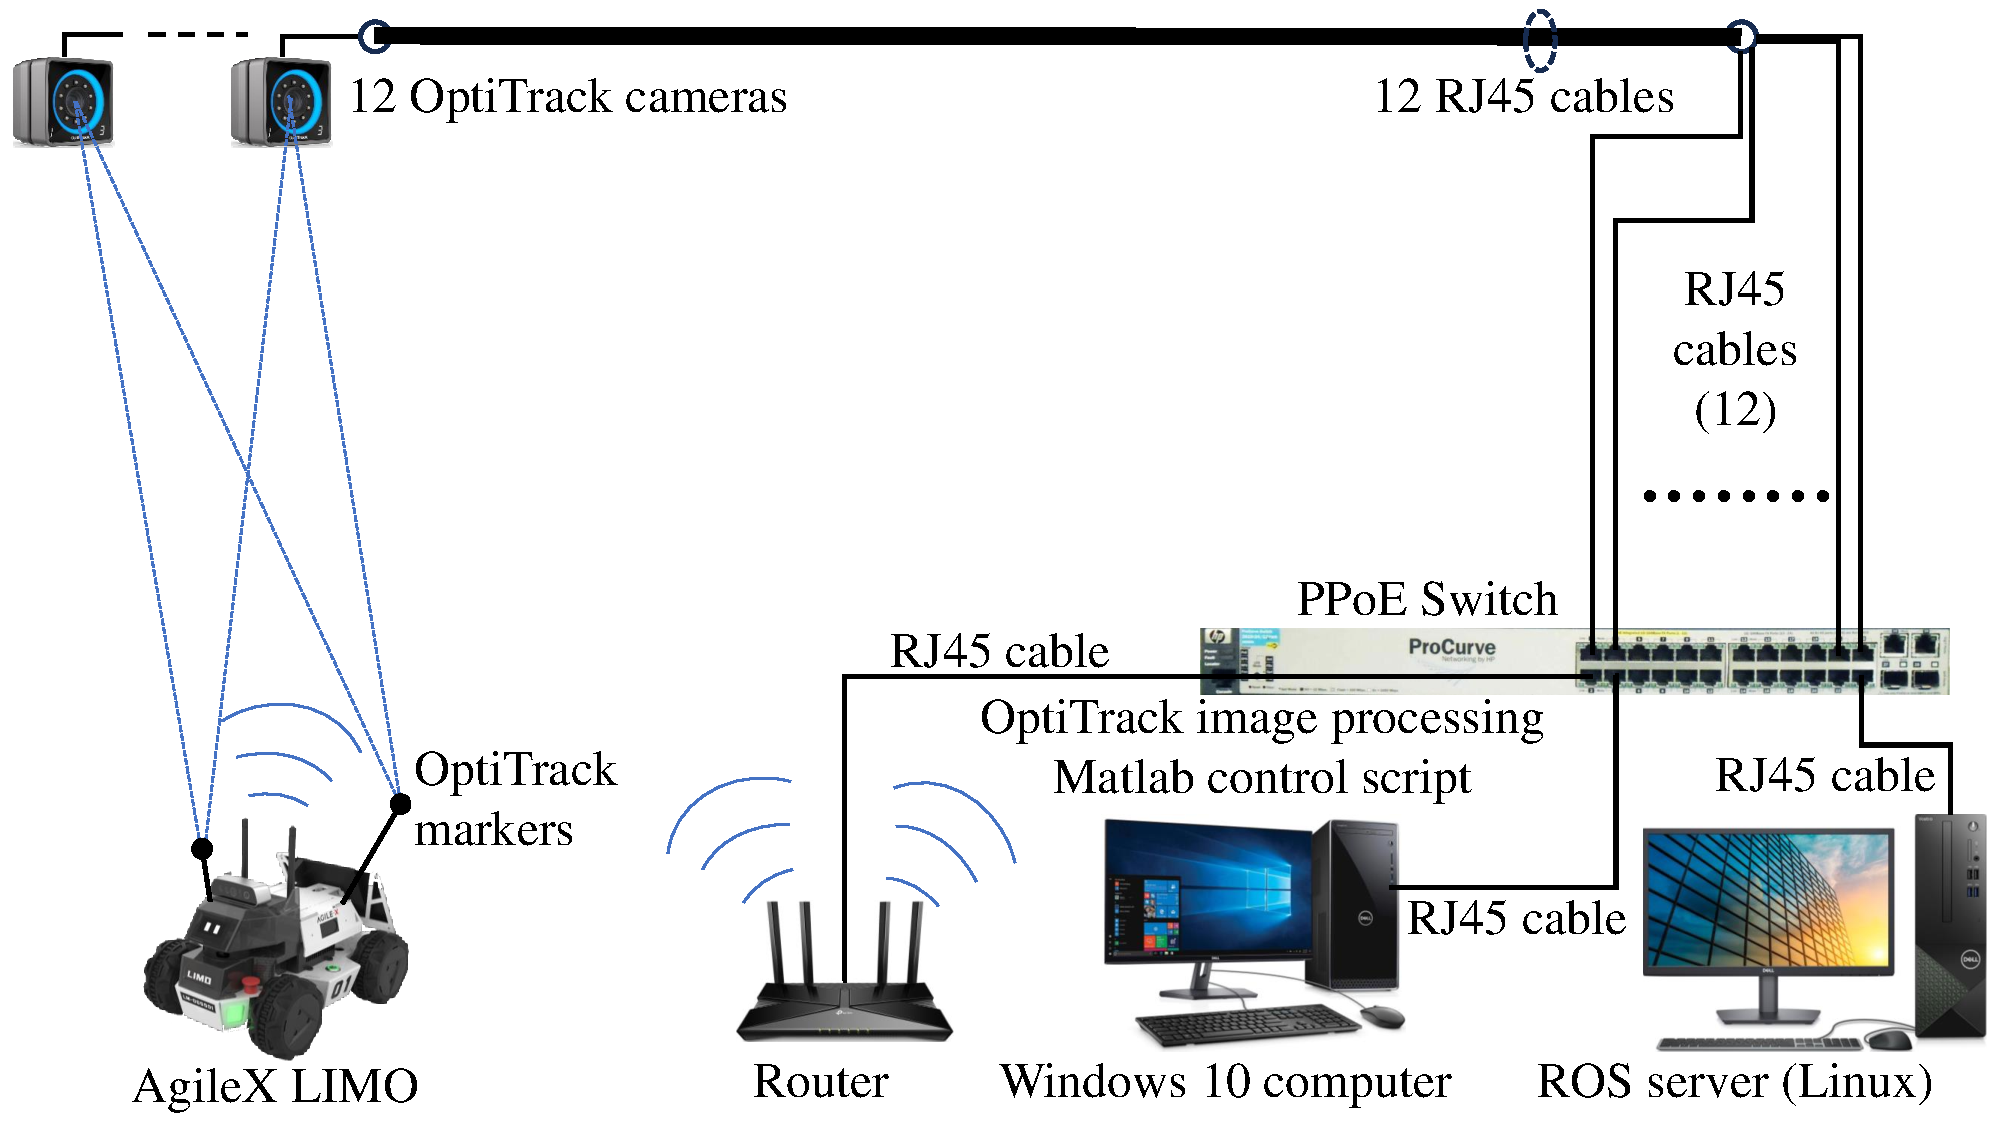
\includegraphics[width=0.8\linewidth]{OptitrackArenaNovaLIMO.pdf}
         \source
         \label{fig:ArenaLAB-AIR}
     \end{figure}
    
    Este computador rodando o \textit{Motive} também se conecta, via uma rede local (não conectada à internet), com outro computador rodando Linux (Ubuntu 18.04) com o ROS Melodic instalado, o que permite que os dados capturados pelas câmeras e processados pelo \textit{Motive} sejam disponibilizados na rede do sistema ROS ao utilizar o pacote \textit{vrpn\_client\_ros}, que estabelece uma comunicação através do protocolo VRPN (\textit{Virtual-Reality Peripheral Network}). Estes pacotes permitem que a posição e a orientação dos objetos e corpos rígidos criados no \textit{Motive} e detectados sejam publicados em tópicos específicos e utilizados por outros pacotes ROS conectados à mesma rede.


\section{Plataforma Robótica LIMO}
\label{sec:Plataforma_LIMO}

    Como plataforma móvel principal foi utilizado o robô móvel terrestre \textit{Limo}, desenvolvido pela \textit{Agilex Robotics}\cite{site:Agilex_Robotics}. Esta é uma plataforma versátil, contando com quatro diferentes modos de operação (diferencial, com esteiras, omnidirecional e \textit{Ackermann}) e equipada com sensores de percepção ativos, contando com um sensor laser do tipo \textit{LiDar} e uma câmera de profundidade, imprescindíveis para a execução de tarefas de mapeamento e localização do robô no seu entorno.

    \subsection{Recursos Computacionais}
    \label{sec:Recursos_LIMO}
        O robô LIMO possui boa capacidade computacional a bordo e sensores adequados para estudos relacionados a navegação autônoma, SLAM, mapeamento, planejamento de trajetórias, desvio de obstáculos, etc. Sua bateria de 12V e 5200mAh fornece autonomia de 40 min de funcionamento ativo e até 2 horas em \textit{stand-by}. A Tabela \ref{tab:sensors_limo} mostra uma lista de alguns sensores/características desse robô.

        \begin{table}[htb]
        \centering        
        \caption{Lista de Sensores e características do LIMO}
            \resizebox{0.8\columnwidth}{!}{ % Resize to the column width
                \setlength{\extrarowheight}{4pt}            
                \begin{tabular}{|l|r|}
                     \hline
                     \textbf{Item} & \textbf{Description}\\ 
                     \hline
                     Overall dimension & $322\ mm\times220\ mm\times251\ mm$\\ \hline
                     Main Board & NVIDIA Jetson Nano (4G)\\ \hline
                     Operating system & Ubuntu 18.04\\ \hline
                     Laser sensor & YDLiDAR EAI X2L\\ \hline
                     Depth camera & ORBBEC Astra+\\ \hline
                     IMU & HI226\\ \hline
                     Voice module & iFlytek voice assistant/Google assistant\\ \hline
                     Speakers & Left and Right, dual channels (2x2W)\\ \hline
                     USB hub & One type-C plus two 2.0 ports \\ \hline
                     Front display & 1.54 inch 128x64 white OLED display \\ \hline
                     Rear display & 7 inches 1024x600 IPS touch screen\\ \hline
                     Communication & Wi-Fi and Bluetooth 5.0 \\ \hline
                     No-load maximum speed & $\pm\ 1\ m/s,$ with no payload\\ \hline
                     Battery & 12 V Li-ion, 5200 mAh\\ \hline
                     Battery working time & 40 minutes \\ \hline
                     Battery standby time & 2 hours \\ 
                     \hline
                \end{tabular}
            }
        \source[Adaptado de \cite{limoUserManual}]
        \label{tab:sensors_limo}
    \end{table}

        A placa principal, uma Nvidia Jetson Nano, é um computador de pequeno porte poderoso capaz de suportar aplicações diversas assim como aplicações de IA de nível básico. Ela possui uma CPU Quad-Core ARM57 de 64 bits rodando a 1,43 GHz, 4 GB de memória RAM LPDDR4 e uma GPU Nvidia Maxwell de 128 núcleos, capaz de decodificação de vídeo em resolução 4K a 60 quadros por segundo. A placa possui um conector Ethernet Gigabit para acesso rápido à internet, saída HDMI, 4 portas USB 3.0, que permitem a conexão de vários dispositivos, e uma porta USB 2.0 Micro-B para alimentação.

        O chassi do LIMO é feito de chapas metálicas, pesa cerca de 4,8 kg e suporta até 4 kg de carga útil. Além disso, essa estrutura pode ser expandida para integrar uma unidade de processamento mais poderosa ou outros dispositivos de sensoriamento. Ou seja, o hardware nativo do LIMO é expansível, o que o torna ainda mais interessante para pesquisa/aplicações. O robô também conta com um módulo Bluetooth 5.0 embutido para conexão com um aplicativo móvel disponível para Android. O LIMO e a placa Jetson Nano estão diretamente conectados por meio de uma interface UART, e a placa pode controlar o chassi através dessa interface. O hub USB fornece 2 interfaces USB e 1 interface Tipo C, todas operando sob o protocolo USB2.0. A tela traseira é conectada ao hub USB através da interface USB2.0 e possui função de toque.

        A placa Nvidia Jetson Nano executa o Ubuntu 18.04, e utiliza o SDK Nvidia JetPack, que contém bibliotecas para aprendizado profundo, visão computacional, gráficos e multimídia. O driver do LIMO, responsável pela comunicação computador de bordo-chassis, foi desenvolvido usando o sistema ROS (Robot Operating System), o que facilita a interação com outros sistemas ROS ao realizar tarefas de forma autônoma. Ele possui duas versões, em C++ e em Python, ambas podendo controlar o movimento do robô. A versão em Python está disponível no Python Package Index (PyPI)~\cite{limoRosPy}, e pode ser baixada usando o comando \texttt{pip}. A versão em C++ está disponível no Github \cite{limoRos1}.


    \subsection{Sensores}
    \label{sec:Sensores_LIMO}
        Como mostra a Tabela~\ref{tab:sensors_limo}, o LIMO possui um sensor LiDAR e uma câmera RGBD. O LiDAR, um YDLIDAR X2, é um sensor laser 2D de 360$^\circ$ que opera com frequência de varredura de 3 kHz e frequência de escaneamento de 6 Hz, com um alcance de até 8 metros em ambientes internos. 
        A câmera de profundidade ORBBEC ASTRA+ utiliza tecnologia de imagem 3D por luz estruturada binocular. Ela contém uma câmera RGB e uma câmera infravermelha, e pode medir profundidades de 0,3 a 3 metros, com uma precisão de 6 mm na faixa de 1 m e um atraso de 30 a 45 ms. Sua resolução máxima de mapa de profundidade é de 640x400 pixels e sua resolução máxima de mapa de cores é de 1920x1080 pixels, ambos a 30 quadros por segundo.
    
        A Unidade de Medição Inercial (IMU) HI226 de 6 graus de liberdade (6DoF) embarcada no LIMO combina um acelerômetro triaxial, um giroscópio triaxial e um microprocessador, permitindo adquirir dados de movimento em três eixos (X, Y e Z) com alta precisão (±2000°/s para o giroscópio e até ±8g para o acelerômetro), fornecendo excelente desempenho em diversas condições operacionais. Ela funciona à frequência máxima de saída, 100Hz, e utiliza algoritmos avançados de fusão de dados, podendo fornecer, simultaneamente, velocidades angulares e acelerações nos três eixos, quatérnions e ângulos de Euler, com pouca distorção de fase. Os erros (RMS) de inclinação e guinada são de 0,8° estáticos e 2,5° dinâmicos.


    \subsection{Controle do LIMO no modo Diferencial}
    \label{sec:Controle_Dif_LIMO}
    
        O controlador cinemático utilizado para o modo diferencial do LIMO é apresentado a seguir, baseado no controlador diferencial apresentado na seção \ref{sec:Modelo_Robos_Diferenciais}.
        
        Como o LIMO apresenta controladores de baixo nível incorporados ao robô, estes já convertem os comandos de velocidade recebidos em comandos de rotação das rodas, portanto precisamos apenas desenvolver um controlador de alto nível que calcule a velocidade longitudinal e a velocidade angular que desejamos que o robô desenvolva para atingir o objetivo. Consequentemente, o sinal de controle de alto nível utilizado é um vetor de velocidades $\begin{bmatrix}v & \omega \end{bmatrix}^{T}$.
        
        Os sensores do sistema provêm a última posição $\bs{x_c}$ do robô, então utiliza-se uma lei de controle \textit{feedforward} e \textit{feedback} proporcional, calculando-se o erro de posição do robô e a velocidade desejada do robô no objetivo:
        \begin{equation}
            \dot{\bs{x}}_{c,ref} = \dot{\bs{x}}_{c,des} + \bs{\kappa}(\bs{x}_{c,des} - \bs{x}_c),
            \label{eq:ff_fb_law_limo}
        \end{equation}
        em que $\bs{\kappa}$ é uma matriz diagonal definida positiva, $\dot{\bs{x}}_{c,des}$ é o vetor de velocidades desejadas e $\dot{\bs{x}}_{c,ref}$ é o vetor de velocidades que o robô deve executar no referencial inercial do mapa ou do mundo.
    
        Como visto na seção \ref{sec:Modelo_Robos_Diferenciais}, o modelo cinemático do robô diferencial, \( \bs{x}_c = \bs{H} \bs{u} \), é dado pela equação
        
        \begin{equation}
            \begin{bmatrix} \dot{x}_c \\ \dot{y}_c  \end{bmatrix} = \begin{bmatrix} \cos{\psi} & -a \sin{\psi} \\ \sin{\psi} & a \cos{\psi}   \end{bmatrix} \begin{bmatrix} v \\ \omega    \end{bmatrix}
            \label{eq:kinematics_differential_limo}
        \end{equation}
        
        e podemos obter o controlador cinemático diretamente pela cinemática inversa \cite{Sarcinelli-Filho2023_4}, tal que $\bs{u} = \bs{H}^{-1} \dot{\bs{x}}_{c,ref}$, ou seja,
        
        \begin{equation}
           \begin{bmatrix} v \\ \omega    \end{bmatrix}
           =  
           \begin{bmatrix} \cos{\psi} & \sin{\psi} \\ -\frac{1}{a}\sin{\psi} & \frac{1}{a} \cos{\psi}   \end{bmatrix} 
           \begin{bmatrix}\dot{x}_{c,ref} \\ \dot{y}_{c,ref}   \end{bmatrix}
           \label{eq:kinematic_controller_differential_limo}
        \end{equation}
        
        onde $v$ e $\omega$ são, respectivamente, as velocidades linear e angular no sistema de coordenadas do robô e, consequentemente, os sinais de controle que são enviados para controlá-lo.
    


\section{ROS - Robot Operating System}
\label{sec:ROS}

    

    \subsection{Pacotes ROS e Launchers do LIMO}
    \label{sec:ROS_LIMO}
            
        A Agilex fornece pacotes do LIMO contendo o \textit{driver} C++, arquivos de configuração, \textit{launchers} ROS e modelos URDF em seu repositório oficial no GitHub~\cite{GithubAgilex} para ambas as versões do ROS \cite{limoRos1,limoRos2}. O pacote \texttt{limo\_base} contém o \textit{driver} em C++, que oferece a interface principal necessária para comunicar com o robô, obter informações de odometria e enviar comandos de velocidade. O \textit{launcher} ROS para inicializar o driver é o \texttt{limo\_base.launcher}.
        
        O pacote \texttt{limo\_bringup} oferece diversos \textit{launchers} para inicializar os recursos disponíveis no robô. O \textit{launcher} \texttt{limo\_start.launch} inicializa o \texttt{limo\_base} e o LiDAR, além de definir a árvore de transformadas entre a base do robô, a câmera, a IMU e o laser. Este pacote também contém outros \textit{launchers} para execução de algoritmos de mapeamento, navegação, visualização, entre outros.
    
        Como observação, no pacote ROS \texttt{limo\_base} fornecido pelo fabricante, o comando de velocidade linear $v$ e o comando de velocidade angular $\omega$ são publicados sob o tópico \texttt{cmd\_vel}, e essas velocidades devem ser atribuídas em \texttt{linear.X} e \texttt{angular.Z}, respectivamente.

    \subsection{Biblioteca Slam Toolbox}
    \label{sec:SLAM_Toolbox}

    % \add{Apresentação do SLAM\_toolbox: principais funcionalidades, justificativa para a escolha e forma de integração com o sistema de robôs.}
    
    % \add{Detalhamento da integração do SLAM\_toolbox com os demais módulos do sistema (por exemplo, aquisição e fusão dos dados sensoriais, controle do robô).}

    De acordo com \citeonline{Macenski2021}, a SLAM Toolbox nasceu com o foco em lidar com ambientes dinâmicos e de grande escala, como galpões, indústrias ou hipermercados, utilizando os processadores limitados presentes em robôs móveis. Segundo eles, os algoritmos de SLAM \textit{open-source} existentes anteriormente no ambiente ROS não eram capazes de realizar o mapeamento correto de grandes áreas e o único que era capaz de fazê-lo, o \textit{Cartographer}, foi abandonado pelo Google e não recebe mais atualizações e melhorias.

    A SLAM Toolbox foi construída sobre a base do algoritmo Open Karto (da SRI \textit{International}), incorporando técnicas modernas de otimização. Utiliza um método de SLAM baseado em grafos (\textit{graph-based}), em que o mapa é representado por um grafo de poses do robô conectadas por restrições de odometria e detecções de loop (fechamento de ciclo), diferindo dos métodos baseados em filtros de Bayes (ex.: filtro de partículas do GMapping). Este método permite maior eficiência de recursos computacionais, especialmente enquanto realiza a construção de mapas em larga escala.

% ------------
    \subsubsection{Princípio de Funcionamento e Algoritmo}

    Em operação, a SLAM Toolbox executa um nó ROS que se subscreve aos dados de um sensor LiDAR 2D (mensagens do tipo \textbf{LaserScan}) e às transformações de odometria do robô(\textit{frame} odom $\rightarrow$ base\_link), produzindo como saída um mapa ocupacional 2D (\textit{frame} map) e a transformação estimada de localização do robô (map $\rightarrow$ odom). A cada varredura recebida do laser, o algoritmo calcula a pose relativa do robô (integrando a odometria) e associa a ela a leitura correspondente do laser, formando um objeto (\textit{PosedScan}) que é inserido em uma fila de processamento. Conforme o robô se move, novos nós são adicionados a um grafo de poses sempre que o deslocamento ultrapassa certos limiares mínimos de distância e/ou ângulo (parâmetros configuráveis) para garantir mudança significativa. Cada novo nó conecta-se ao anterior por uma aresta de odometria e, adicionalmente, é refinado por casamento de scans (scan matching) com a pose anterior, o que alinha a leitura laser atual com a esperada a partir do mapa em construção. O uso do algoritmo robusto de casamento de laser herdado do Open Karto garante alinhamento preciso das leituras sequenciais.

    Conforme o grafo se constrói, a SLAM Toolbox busca detecções de fechamento de loop (loop closures). Isso ocorre quando uma leitura atual do laser tem alta correlação com partes do mapa já mapeadas anteriormente, indicando que o robô retornou a uma região conhecida. Nesses casos, o algoritmo adiciona arestas no grafo conectando a pose atual com aquela pose passada correspondente (restrição de loop) e então executa uma otimização global do grafo para minimizar os erros acumulados. A otimização é realizada por métodos de mínimos quadrados não lineares; originalmente o Karto usava um otimizador de Sparse Bundle Adjustment, mas na SLAM Toolbox este foi substituído pelo solver Google Ceres, resultando em otimização mais rápida e flexível\cite{Macenski2021}. O sistema foi projetado de forma modular, permitindo inclusive carregar diferentes plugins de solver – por meio de uma interface dinâmica em tempo de execução – possibilitando substituição futura do algoritmo de otimização sem modificar o núcleo do código.

    Uma vez otimizado o grafo (especialmente após um fechamento de loop), todas as poses do robô são ajustadas consistentemente, e o mapa ocupacional é atualizado utilizando as leituras laser armazenadas em cada pose corrigida. Esse processo garante um mapa globalmente consistente, corrigindo distorções à medida que loops são fechados. Em resumo, a SLAM Toolbox segue o paradigma típico de SLAM gráfico: construção incremental do mapa com ajustes retroativos ocasionais via otimização de grafo, ao invés de manter múltiplas hipóteses simultâneas como nos métodos de filtro de partículas.

    Um diferencial importante da SLAM Toolbox é suportar dois modos de operação quanto ao gerenciamento do fluxo de dados: síncrono e assíncrono. No modo síncrono, o nó processa todos os dados de sensor válidos na ordem em que chegam, podendo incorrer em atraso caso a taxa de leitura seja alta ou o processamento intenso (prioriza mapear com o máximo de detalhes). Já no modo assíncrono, o algoritmo processa os dados “o mais rápido possível”, descartando ou pulando leituras se necessário para manter o desempenho em tempo real (prioriza a responsividade). Esses modos permitem ajustar o funcionamento conforme a aplicação: por exemplo, em robôs com poder de computação limitado operando em áreas enormes, o modo assíncrono evita que o SLAM fique para trás em relação ao movimento do robô, enquanto em aplicações de mapping offline pode-se rodar no modo síncrono para utilizar todos os dados disponíveis. Em ambos os casos, o resultado final esperado (um mapa consistente) é equivalente, mas o modo assíncrono traz leve degradação de detalhe temporal para ganhar em robustez de tempo real. Adicionalmente, a biblioteca implementa um modo de operação apenas de odometria a laser (\textit{LiDAR odometry}), no qual é executada a mesma estimação de movimento por casamento de scans mas sem construir um mapa global – ou seja, sem um mapa prévio, o sistema atua como um odômetro local que realiza pequenos fechamentos de loop locais (útil para estimar movimento em tempo real quando não se deseja ainda um mapa completo). Esse modo pode ser entendido como uma forma degenerada de SLAM restrita a um mapa local temporário.

% --------
    
    A biblioteca conta com diversos modos de operação para SLAM e um modo de Localização que também pode ser utilizado para obter odometria através do sensor LiDAR quando nenhum mapa é carregado ao rodar o modo de Localização. 
    
    Utilizaremos o modo de operação online e síncrono da biblioteca para gerar o mapa do laboratório. Este modo de operação analisa todas as medições recebidas do sensor LiDAR, em ordem de recebimento, e faz a correlação entre a última medição recebida e medições anteriores em busca de correlações que permitam a localização do robô no mapa em construção e o fechamento de loops, que ocorrem quando a última medição corresponde bem o suficiente com medições passadas. O fechamento de loop é essencial para o mapeamento correto de ambientes, permitindo que o robô identifique que já esteve naquele local anteriormente.

    
    

    % \add{Descrição da implementação experimental, destacando as etapas de configuração, calibração e execução dos testes.}

    
\section{Detalhes da Implementação do Projeto}

    Para este projeto foi necessário realizar uma pequena modificação na estrutura do LIMO, modificando o local do seu sensor laser, que normalmente encontra-se montado na parte posterior no robô, possibilitando apenas o uso de $180\degree$ do campo de visão do LiDAR. Criou-se então uma plataforma para montagem do sensor laser na parte superior do corpo do robô, a fim de possibilitar o uso completo dos $360\degree$ do campo de visão do LiDAR do robô (Ver Figura \ref{fig:LIMO_Experimento}). 

    \begin{figure}[htb]
        \centering
        \caption{Robô LIMO Modificado para uso do campo de visão total do LiDAR}
        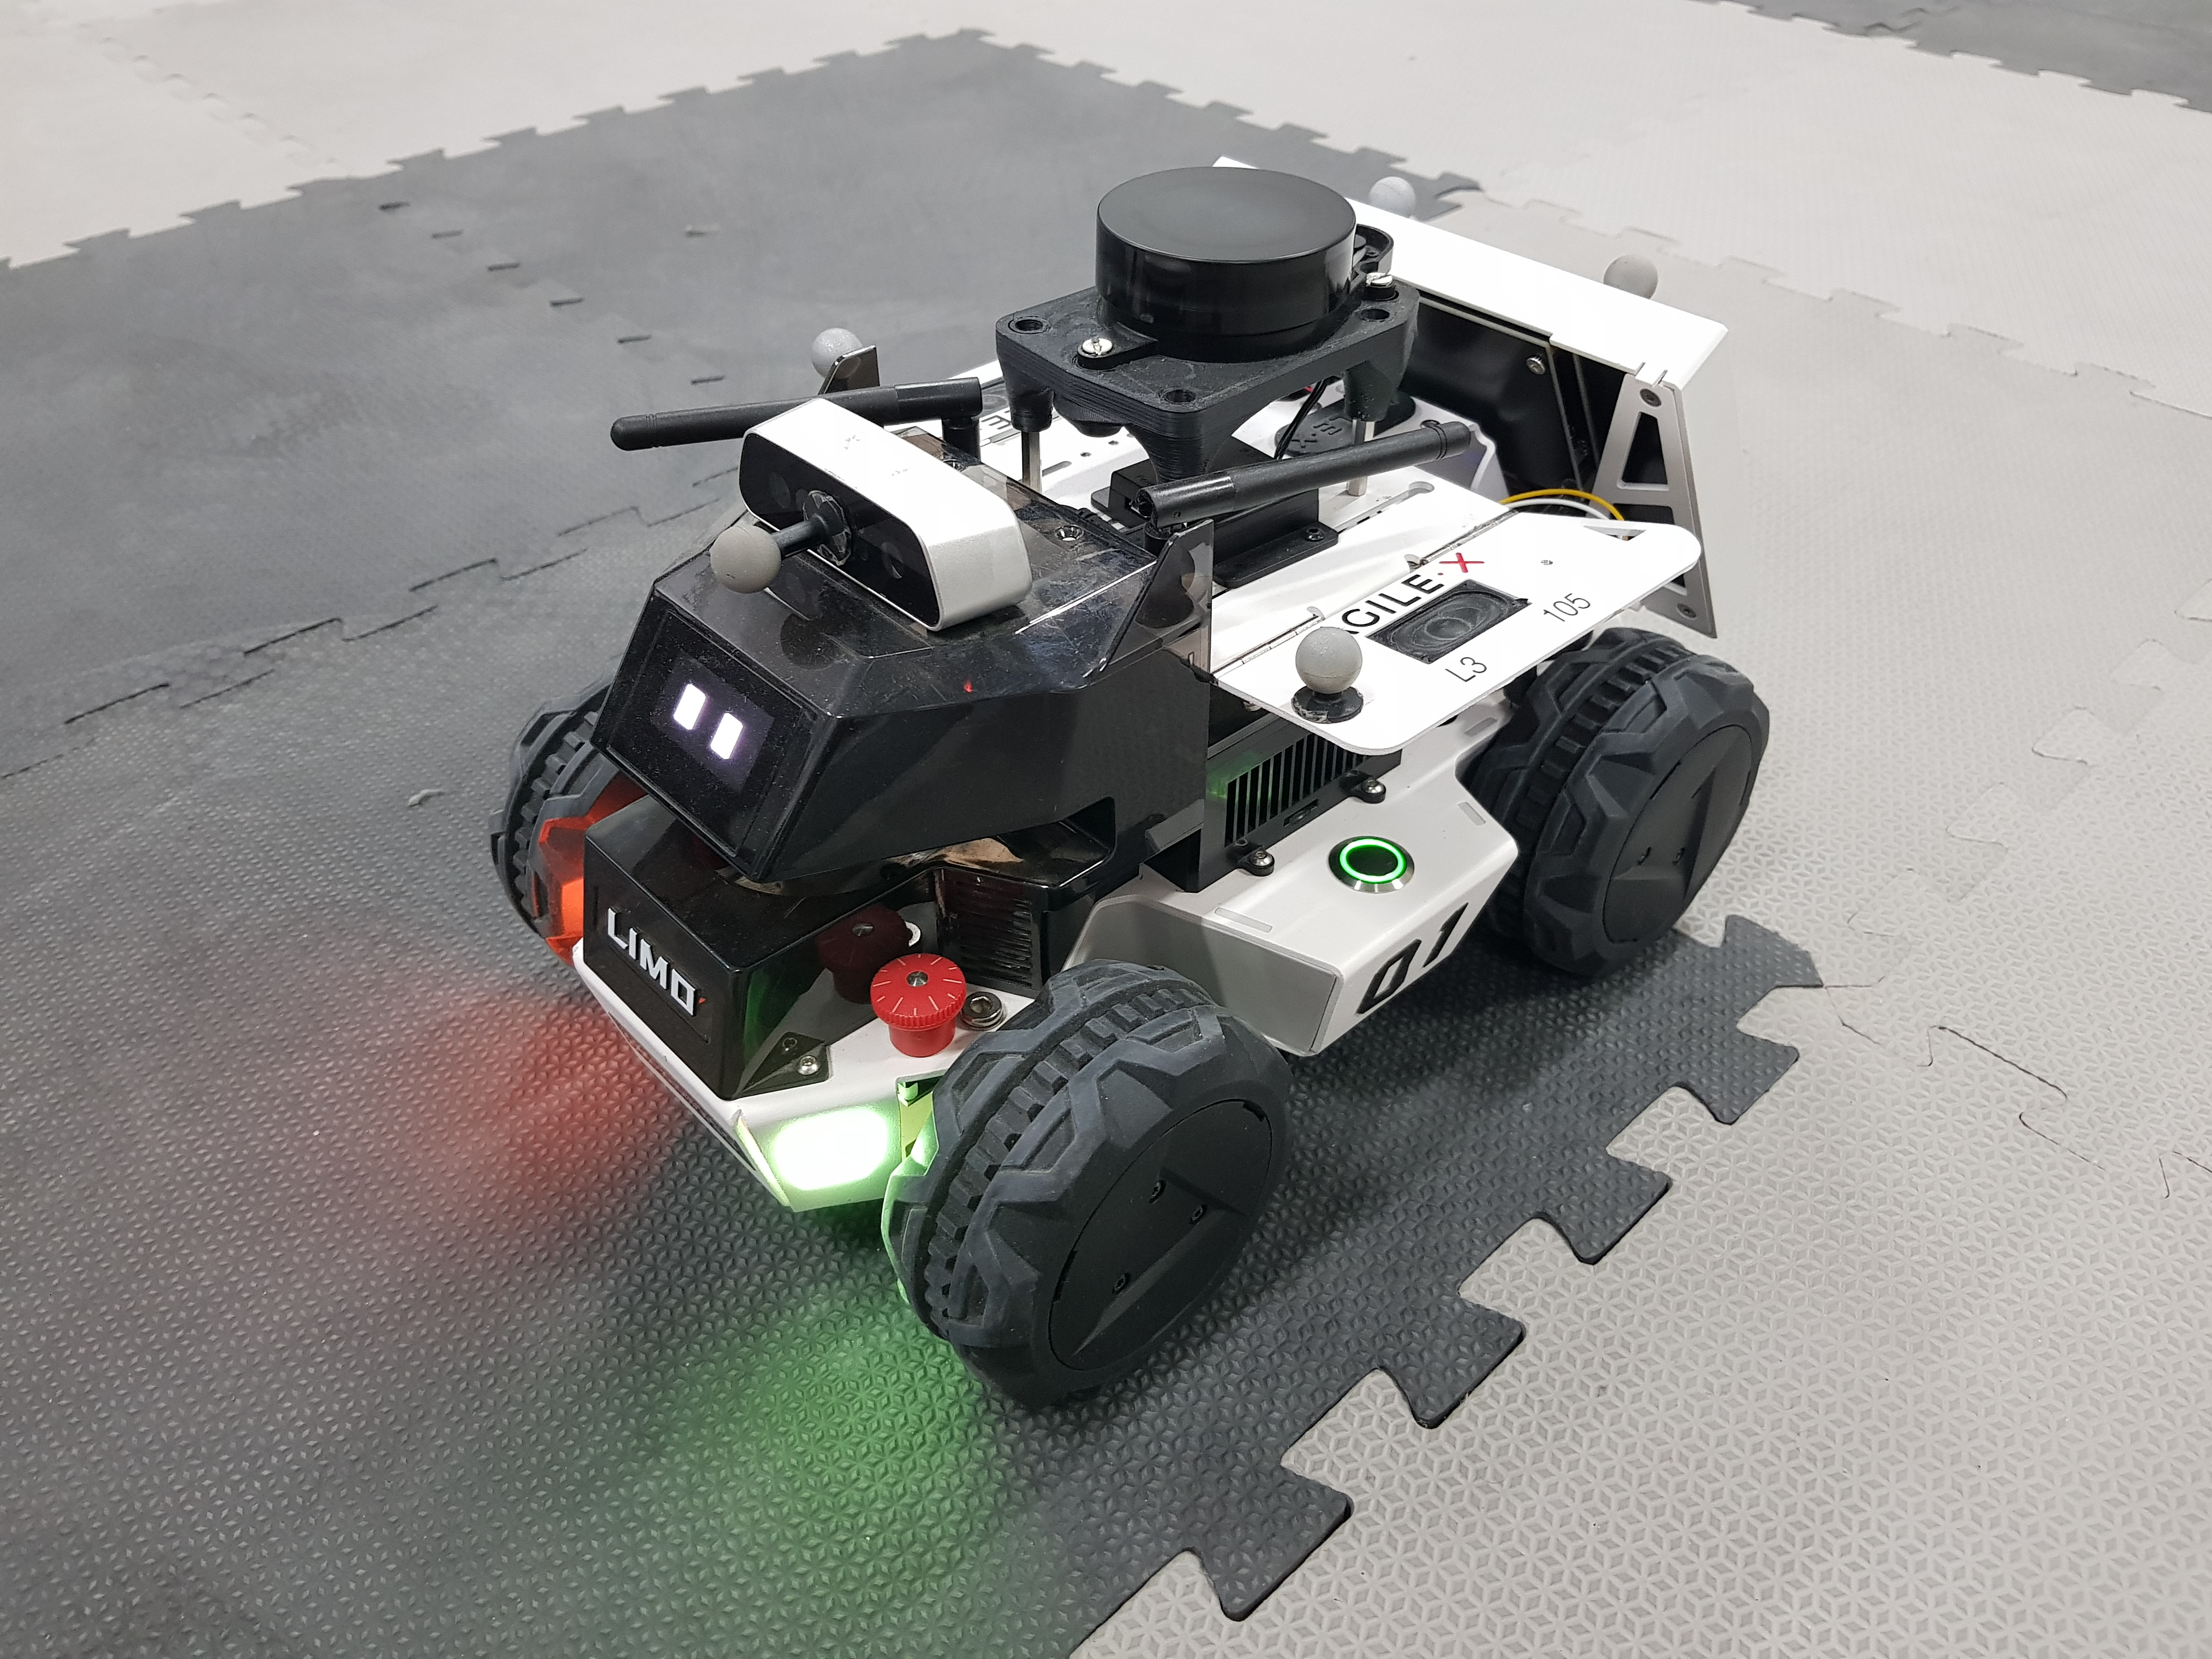
\includegraphics[width=0.8\linewidth]{img/LIMO_EXPERIMENTO.jpg}
        \source
        \label{fig:LIMO_Experimento}
    \end{figure}

    Para realizar o projeto, primeiro foi implementado o controlador para o robô diferencial, seguindo a lei de controle da Equação \ref{eq:ff_fb_law_limo}. O código foi implementado em linguagem C++ e utilizando as bibliotecas do ROS para obtenção dos dados de posição e publicação dos comandos de velocidade.
    
    Também foi implementado um código para publicação da trajetória a ser seguida pelo robô, que calcula os pontos da trajetória em função da frequência de publicação e da velocidade desejada para a trajetória. Este código publica as poses objetivos no tópico /goal e também publica o caminho inteiro em um outro tópico, que pode ser utilizado para tarefas de seguimento de caminho ou para visualização da trajetória e/ou caminho desejado. Todos os códigos implementados estão disponíveis no \textit{Github} \cite{site:Github-SLAM_Research}.

    Para a utilização da SLAM Toolbox para este projeto, realizou-se uma cópia do repositório da SLAM Toolbox\cite{site:Slam_toolbox}. Como utilizamos o ROS 1 no LAB-AIR foi necessário modificar o código da SLAM Toolbox para que a pose do robô obtida a partir do escaneamento do LiDAR fosse publicada também no modo de Localização. A SLAM Toolbox somente publicava as poses corretamente na versão para o ROS 2.

    A SLAM Toolbox expõe ao usuário diversos parâmetros de configuração que podem ser modificados para buscar o melhor desempenho do sistema. Para buscar o melhor funcionamento do sistema junto ao controle utilizado e obter melhores resultados, foi necessário modificar estes parâmetros e realizar diversos testes, rodando diversas vezes o código em modo de slam online e localização para obtenção de resultados mais satisfatórios para o projeto.
    
    Em específico, notou-se durante a implementação do projeto e durante os testes que o robô utilizado apresentava muitos erros de odometria, devido ao problema de deslizamento das rodas no chão, principalmente ao realizar curvas no modo diferencial. Portanto, para obter melhores resultados utilizando a SLAM Toolbox modificou-se a função utilizada para rejeitar valores discrepantes (\textit{outliers}) para uma função \textit{HuberLoss} através do parâmetro \textit{ceres\_loss\_function}.

    Outros parâmetros também foram alterados para que a pose do robô fosse atualizada e publicada com maior frequência pela biblioteca. Os parâmetros \textit{minimum\_time\_interval}, \textit{minimum\_travel\_distance} e \textit{minimum\_travel\_heading} foram reduzidos para que o sistema de controle pudesse funcionar satisfatoriamente.
    

    

% \section{Estrutura do código}

% \begin{itemize}
%     \item \add{Descrição do sistema original proposto e os algoritmos inicialmente planejados.}
%     \item \add{Justificativa das limitações encontradas e da decisão de adotar o SLAM\_toolbox.}
%     \item \add{Detalhamento da integração do SLAM\_toolbox com os demais módulos do sistema (por exemplo, aquisição e fusão dos dados sensoriais, controle do robô).}
%     \item \add{Descrição da implementação experimental, destacando as etapas de configuração, calibração e execução dos testes.}
% \end{itemize}

\fi

%%%%%%%%%%%%%%%%%%%%%%%%%%%%%%%%%%%%%%%%%%%%%%%%%%%%%
%%%%%%%%%%%%%%%%%%%%%%%%%%%%%%%%%%%%%%%%%%%%%%%%%%%%%
%%%%%%%%%%%%%%%%%%%%%%%%%%%%%%%%%%%%%%%%%%%%%%%%%%%%%

\ifisTipoDocumento
    % PG
    \chapter[Alocação de Recursos]{Alocação de Recursos}
    \section{Recursos Materiais}

\textbf{Material bibliográfico.} O material bibliográfico utilizado é composto principalmente por periódicos científicos, artigos e livros. Este material estará disponível para o autor do trabalho das seguintes maneiras: fisicamente, via Biblioteca Central da UFES, e eletronicamente, via rede de internet da UFES, permitindo o acesso ao acervo eletrônico próprio da universidade e ao acervo cujo acesso tenha sido adquirido pela universidade.

\textbf{Base de dados xxxx.}
\input{DataBase}

\section{Recursos Computacionais}

\textbf{Recursos de \textit{Software}}
\input{Software}

\textbf{Recursos de \textit{Hardware}}
\input{Hardware}
\else
    % TCC
    \chapter[Experimentos e Resultados]{Experimentos e Resultados}
    % \begin{itemize}
%     \item \add{Apresentação dos experimentos realizados: descrição dos cenários testados, procedimentos e configurações.}
%     \item \add{Comparação dos resultados do SLAM\_toolbox com os dados do sistema OptiTrack, apresentando gráficos, mapas, trajetórias e análises quantitativas.}
%     \item \add{Discussão dos resultados: análise dos pontos fortes e limitações da solução adotada, implicações para aplicações reais e comparação com os objetivos propostos.}
% \end{itemize}


\label{Cap04}

% \add{
% \textbf{1. \txr{Objetivo do capitulo}}
% Neste capítulo serão apresentados os resultados obtidos.....
% \textbf{2. \txr{Temas a tratar}}
% De tal modo, o capítulo inicia descrevendo o banco de dados utilizado para treinamento e teste das abordagens propostas, 
% também são apresentados todos os resultados obtidos em diferentes etapas do processo, mostrando a evolução obtida a partir da implementação de algumas técnicas apresentadas anteriormente. 
% E por fim, é feita uma análise destes resultados e uma comparação com os resultados obtidos por outros trabalhos semelhantes com o intuito de validar as abordagens propostas.
% }


% ------------------ INICIO ----------------------
Utilizou-se a princípio a biblioteca SLAM Toolbox para criação de um mapa detalhado do laboratório, fazendo o robô percorrer diversos caminhos no interior do laboratório para que o mapa gerado fosse de alta qualidade e representativo do ambiente de testes. O mapa gerado por este método foi salvo e utilizado como mapa para os experimentos de localização do robô utilizando o modo de Localização da SLAM Toolbox. A Figura \ref{fig:Exp_mapa_LABAIR} mostra o mapa gerado, onde os pontos vermelhos conectados por linhas azuis são os nós do grafo com as informações de poses e as linhas azuis são as arestas que definem as restrições entre as poses dos nós. Os pequenos quadrados vermelhos e laranjas no mapa são os pontos medidos pelo sensor LiDAR.

\begin{figure}[htb]
    \centering
    \caption{Mapa do LAB-AIR gerado com a SLAM Toolbox, mostrando os marcadores das posições e conexões do grafo de poses}
    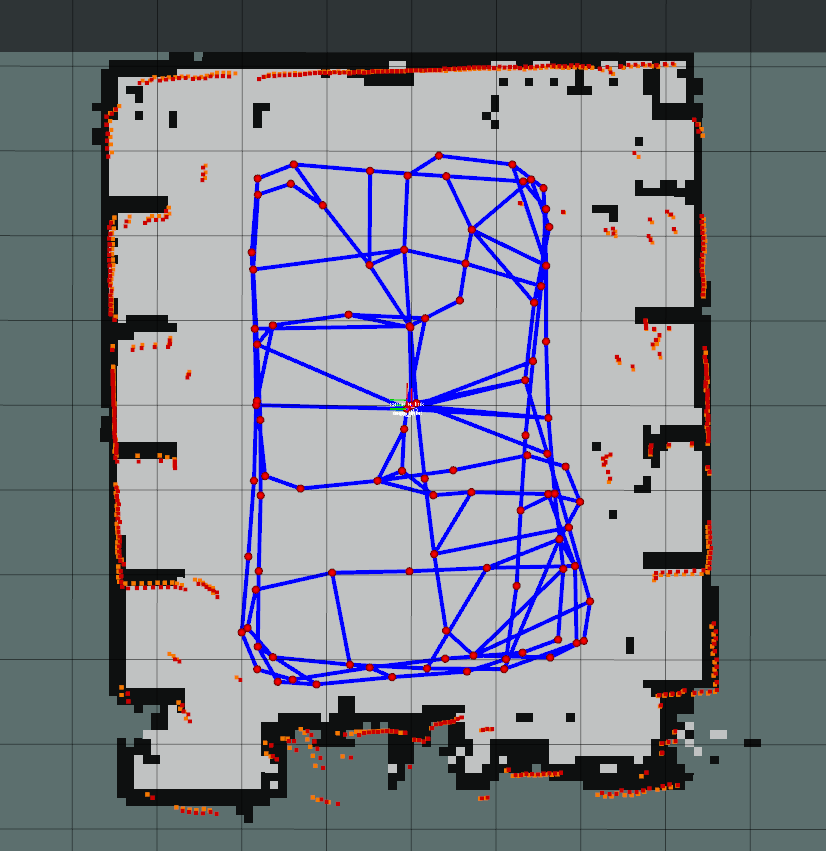
\includegraphics[width=0.8\linewidth]{img/mapa_localizacao.png}
    \source
    \label{fig:Exp_mapa_LABAIR}
\end{figure}

Para verificar o desempenho da tarefa de localização usando a SLAM Toolbox, utilizou-se o controlador definido na Seção \ref{sec:Controle_Dif_LIMO} para guiar o robô em dois tipos diferentes de trajetórias, uma caracterizada por caminhos lineares entre posições específicas no referencial inercial do laboratório, e uma trajetória em formato de Lemniscata de Bernoulli. As duas trajetórias podem ser vistas na Figura \ref{fig:exp_trajetorias}. A trajetória que foi denominada como \ASPASDUPLAS{CASA} foi definida como retas ligando os pontos adjacentes do vetor de pontos mostrados na Tabela \ref{tab:traj_CASA} abaixo.

\begin{table}
    \centering
    \caption{Pontos que definem a trajetória \ASPASDUPLAS{CASA} usada nos experimentos.}
    \setlength{\extrarowheight}{2pt}
    \begin{tabular}{|c|cc|}
        \hline
        n & x & y \\
        \hline
        1 & -1.5 & \phantom{-}1.5\\
        2 & -1.5 & -1.5 \\ 
        3 & \phantom{-}1.5 & \phantom{-}1.5 \\ 
        4 &  \phantom{-}1.5 & -1.5 \\ 
        5 & -1.5 & \phantom{-}1.5 \\
        6 &  \phantom{-}1.5 & \phantom{-}1.5 \\
        7 &  \phantom{-}2.0 & \phantom{-}0.0 \\
        8 &  \phantom{-}1.5 & -1.5 \\
        9 &  -1.5 & -1.5 \\ \hline
    \end{tabular}
    
    \label{tab:traj_CASA}
    \source
\end{table}


% \begin{equation}
%     \begin{bmatrix}
%         -1.5 & \phantom{-}1.5\\ 
%         -1.5 & -1.5 \\ 
%         \phantom{-}1.5 & \phantom{-}1.5 \\ 
%          \phantom{-}1.5 & -1.5 \\ 
%         -1.5 & \phantom{-}1.5 \\
%         \phantom{-}1.5 & \phantom{-}1.5 \\
%         \phantom{-}2.0 & \phantom{-}0.0 \\
%         \phantom{-}1.5 & -1.5 \\
%         -1.5 & -1.5
%     \end{bmatrix}
% \end{equation}

\begin{figure}[htb]
    \centering
    \caption{Trajetórias Desejadas dos Experimentos}
    \begin{subfigure}[b]{0.4\textwidth}
        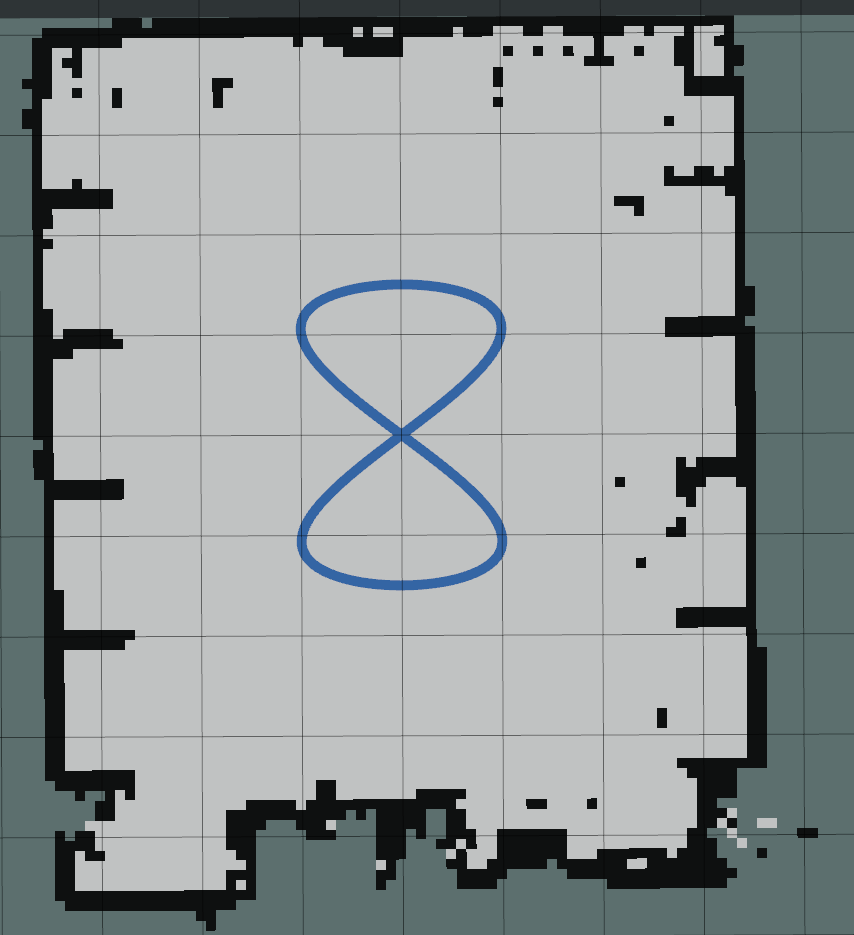
\includegraphics[width=\textwidth]{img/Trajetoria_Lemniscata.png}
        \caption{Trajetoria em Lemniscata de Bernoulli}
    \end{subfigure}
    \hspace{0.1\textwidth}
    \begin{subfigure}[b]{0.4\textwidth}
        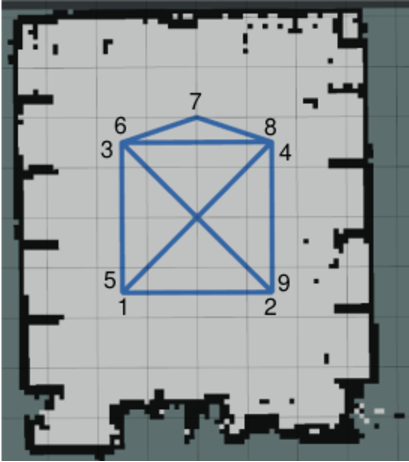
\includegraphics[width=\textwidth]{img/Trajetoria_Casa_num.pdf}
        \caption{Trajetória Linear \ASPASDUPLAS{CASA}}
    \end{subfigure}
    \label{fig:exp_trajetorias}
    \sourceParbox[0.8\linewidth]
\end{figure}

A segunda trajetória realizada no segundo e quarto experimentos foi uma trajetória em formato de lemniscata de Bernoulli, caracterizada pelas equações:

\begin{equation}
\label{eq:lemniscata}
    \bs{x}_{des}=\begin{bmatrix} x_{des}=r_x\cos{\omega t} \\ y_{des}=r_y\sin{2 \omega t} \end{bmatrix}
\end{equation}

com $r_x = 1.5m$, $r_y = 1.0m$ e $\omega = 0.20\ rad/s$. A velocidade desejada da trajetória é obtida pela derivada da equação anterior, ou seja:

\begin{equation}
    \dot{\bs{x}}_{des}=\begin{bmatrix} \dot{x}_{des} = -r_x \omega \sin{\omega t} \\
    \dot{y}_{des}=r_y 2\omega\cos{2 \omega t} \end{bmatrix}
\end{equation}

Para avaliar o desempenho do sistema com o referencial do OptiTrack realizou-se 4 experimentos de controle de trajetória para cada uma das duas trajetórias definidas, usando primeiro informações provindas do sistema Optitrack para obter a pose do robô e posteriormente utilizando apenas as poses obtidas pela SLAM Toolbox. Os dois primeiros experimentos serviram para analisar o desempenho do controlador implementado utilizando o sistema de referência para as duas trajetórias, a fim de obter o desempenho do controlador para o sistema ideal.

Em todos os 4 experimentos armazenou-se tanto os dados de pose provindas do OptiTrack quanto da SLAM Toolbox, os sinais de controle calculados tanto com os dados de pose do OptiTrack quanto da SLAM Toolbox e a trajetória a ser seguida a fim de gerar os gráficos apresentados neste capítulo. A pose inicial do robô foi resetada ao início de cada experimento, mantendo o ponto $(x,y)=(0.0 ,0.0)$ do referencial inercial do laboratório como posição inicial e orientação inicial sempre paralela ao eixo $X$ ($\psi = 0\degree$).

O primeiro experimento realizado foi o controle de trajetórias lineares que formam uma figura de casa, utilizando a pose provinda do sistema OptiTrack para executar o controle. A trajetória realizada e a trajetória desejada podem ser vistas na Figura \ref{fig:Exp1_Trajetoria_VRPN_LINEAR}. Pode-se notar que a trajetória realizada pelo robô segue em grande parte a trajetória desejada, com alguns erros de seguimento da trajetória em pontos mais críticos de viradas mais bruscas e no início do experimento, quando o robô sai da origem do plano cartesiano e corre atrás do ponto da trajetória que está em movimento. A Figura \ref{fig:Exp1_XY_vs_tempo} mostra a evolução das posições obtidas do OptiTrack (\ASPASIMPLES{vrpn}) e da SLAM Toolbox(\ASPASIMPLES{slam} durante o experimento.

\begin{figure}[htb]
    \centering
    \caption{Experimento 1: Trajetoria Realizada}
    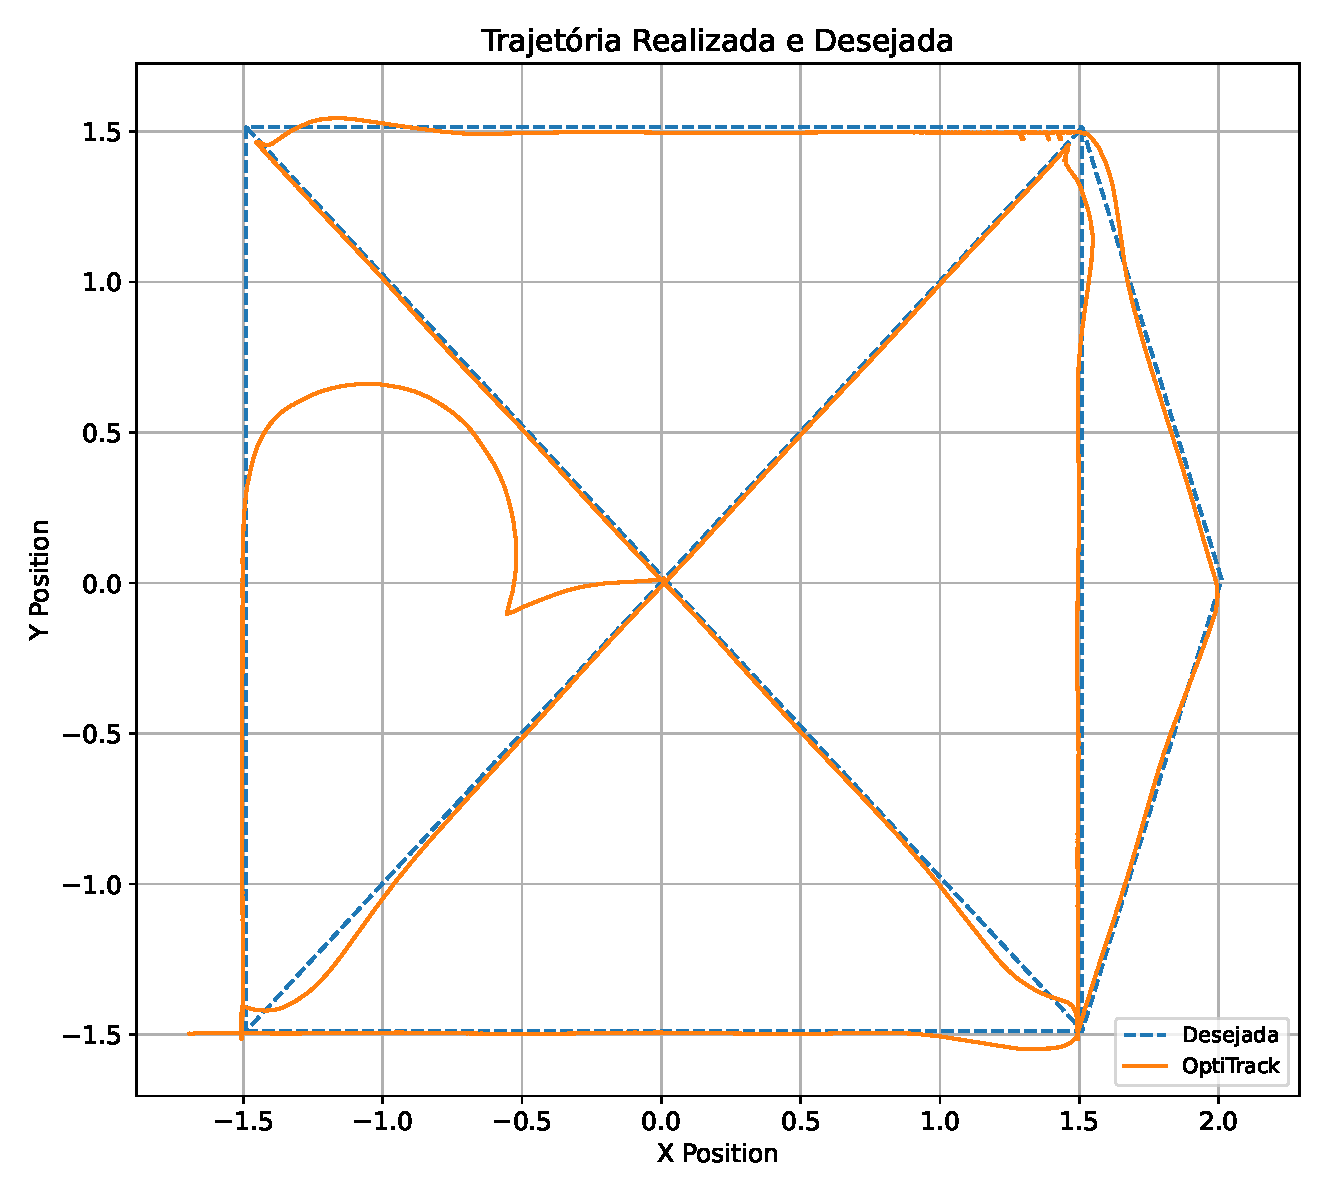
\includegraphics[width=0.8\linewidth]{img/Resultados/Exp1_VRPN_Control_LINEAR/Trajetoria.pdf}
    \label{fig:Exp1_Trajetoria_VRPN_LINEAR}
    \source
\end{figure}

% \begin{figure}[htb]
%     \centering
%     \caption{Trajetória realizada pelo robô no primeiro experimento}
%     \begin{subfigure}[b]{0.49\textwidth}
%          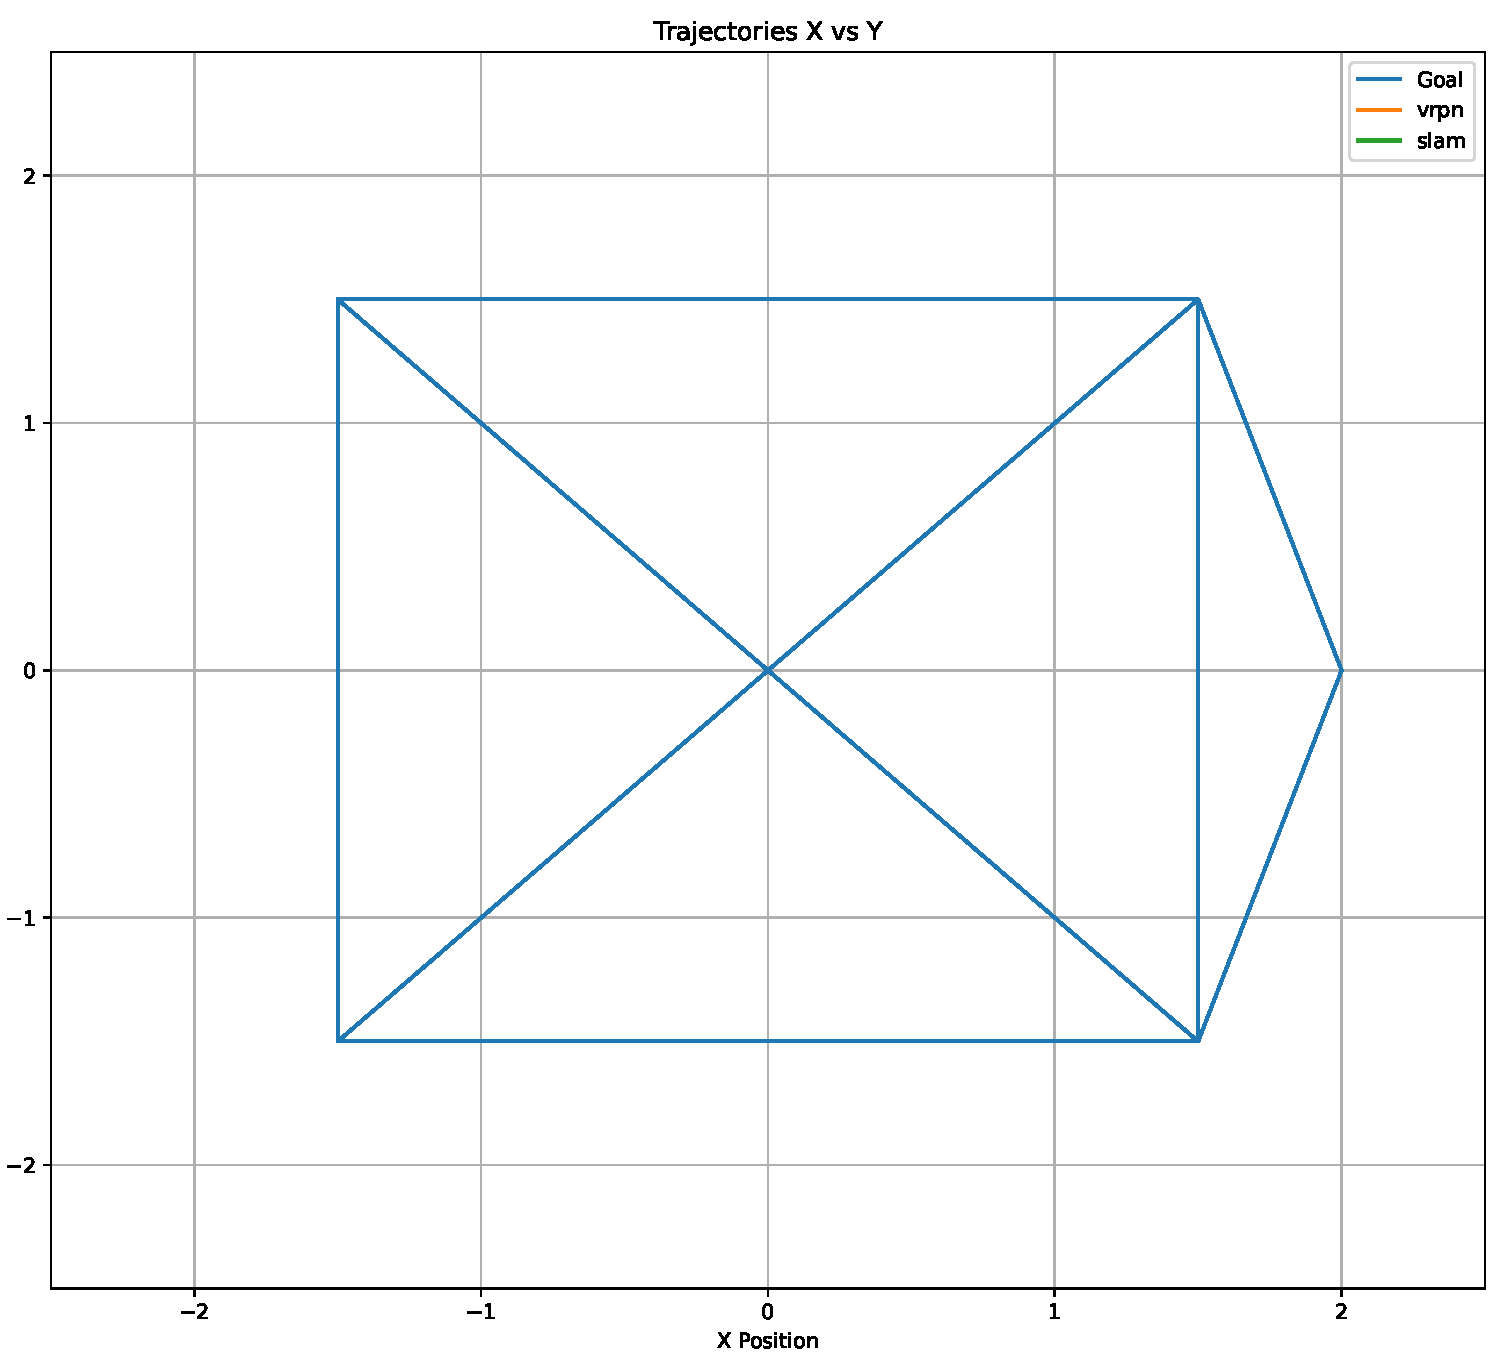
\includegraphics[width=\textwidth]{img/Resultados/Exp1_VRPN_Control_LINEAR/Trajetoria_Goal.pdf}
%     \end{subfigure}
%     \begin{subfigure}[b]{0.49\textwidth}
%         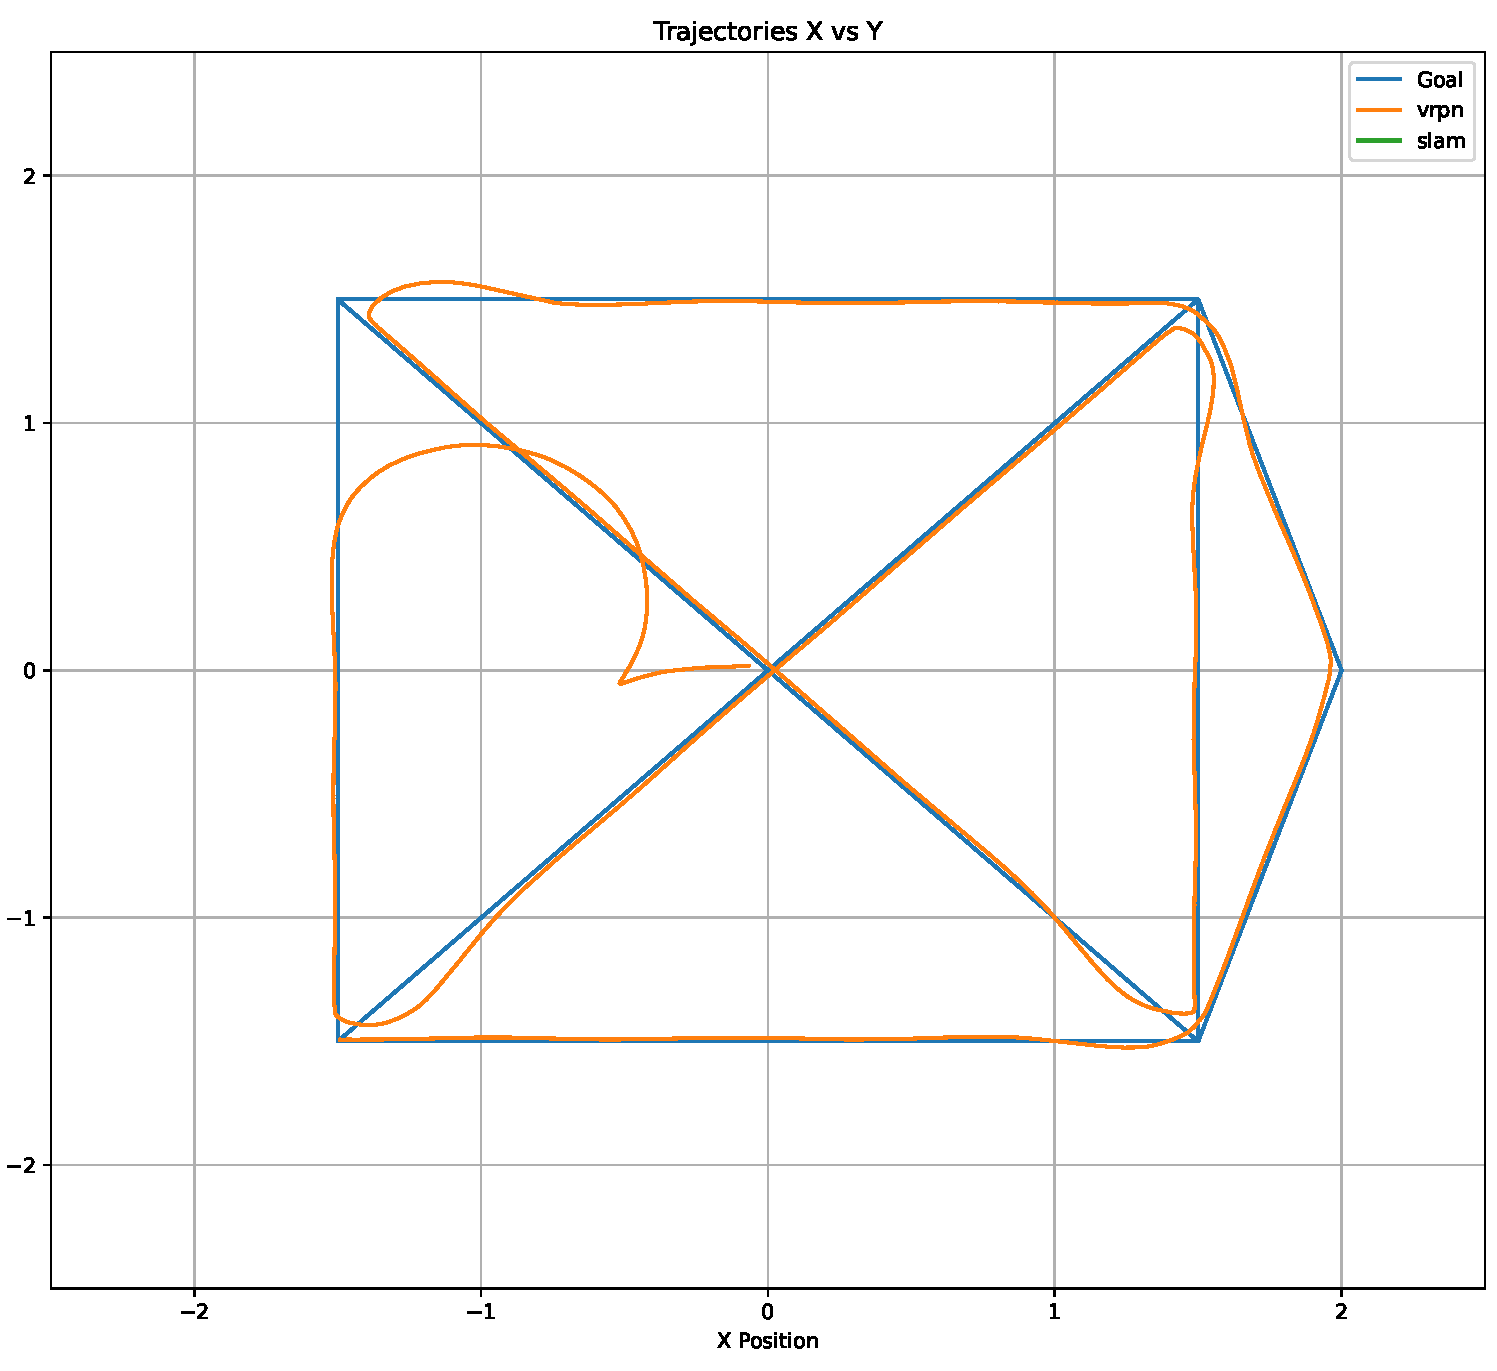
\includegraphics[width=\textwidth]{img/Resultados/Exp1_VRPN_Control_LINEAR/Trajetoria_VRPN_Goal.pdf}
%     \end{subfigure}
%     \source
%     \label{fig:Exp1_Trajetoria_VRPN_LINEAR}
% \end{figure}

% \begin{figure}[htb]
%     \centering
%     \caption{Trajetória Realizada + Pose obtida pela SLAM Toolbox}
%     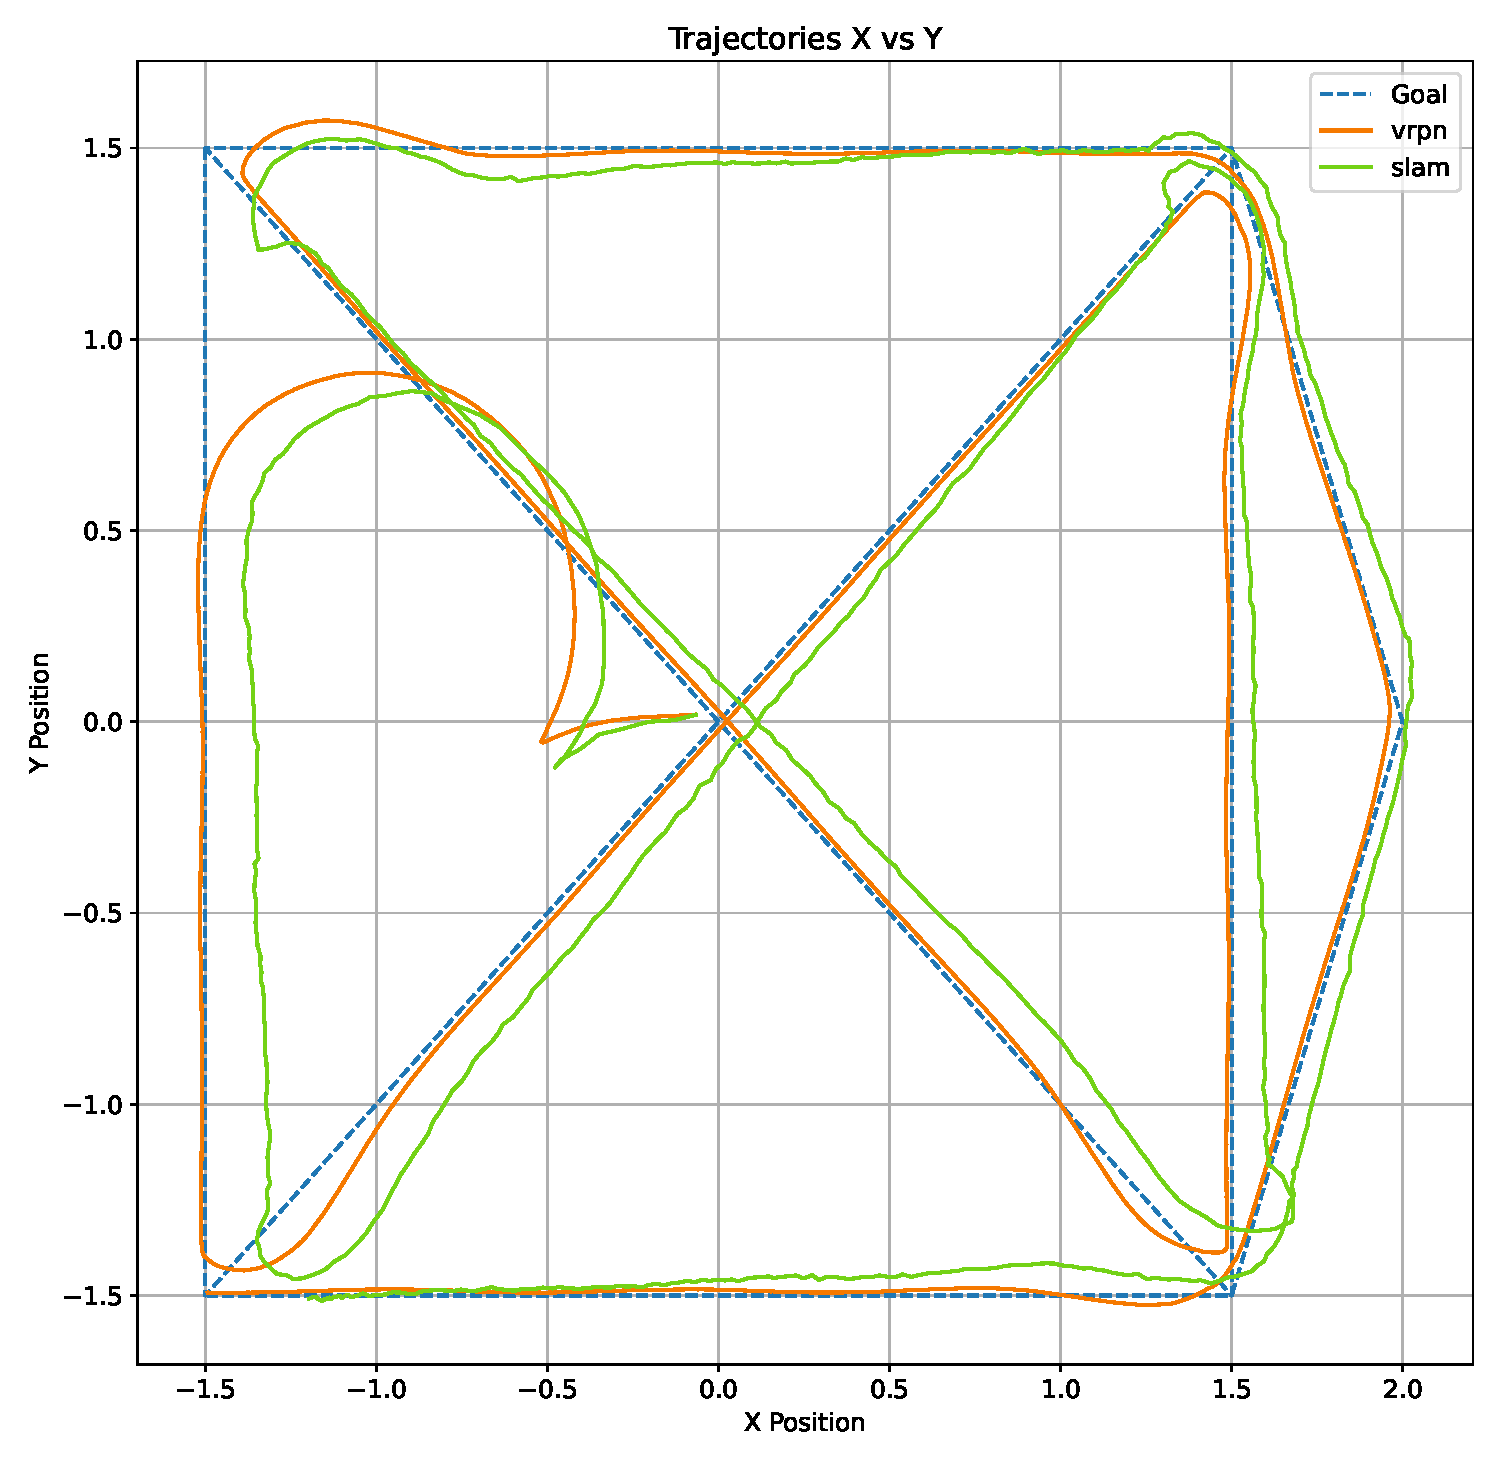
\includegraphics[width=0.8\linewidth]{img/Resultados/Exp1_VRPN_Control_LINEAR/Trajetoria_ALL.pdf}
%     \label{fig:Exp1_Trajetoria_All}
% \end{figure}

\begin{figure}[htb]
    \centering
    \caption{Evolução das coordenadas $x$ e $y$ no Experimento 1}
    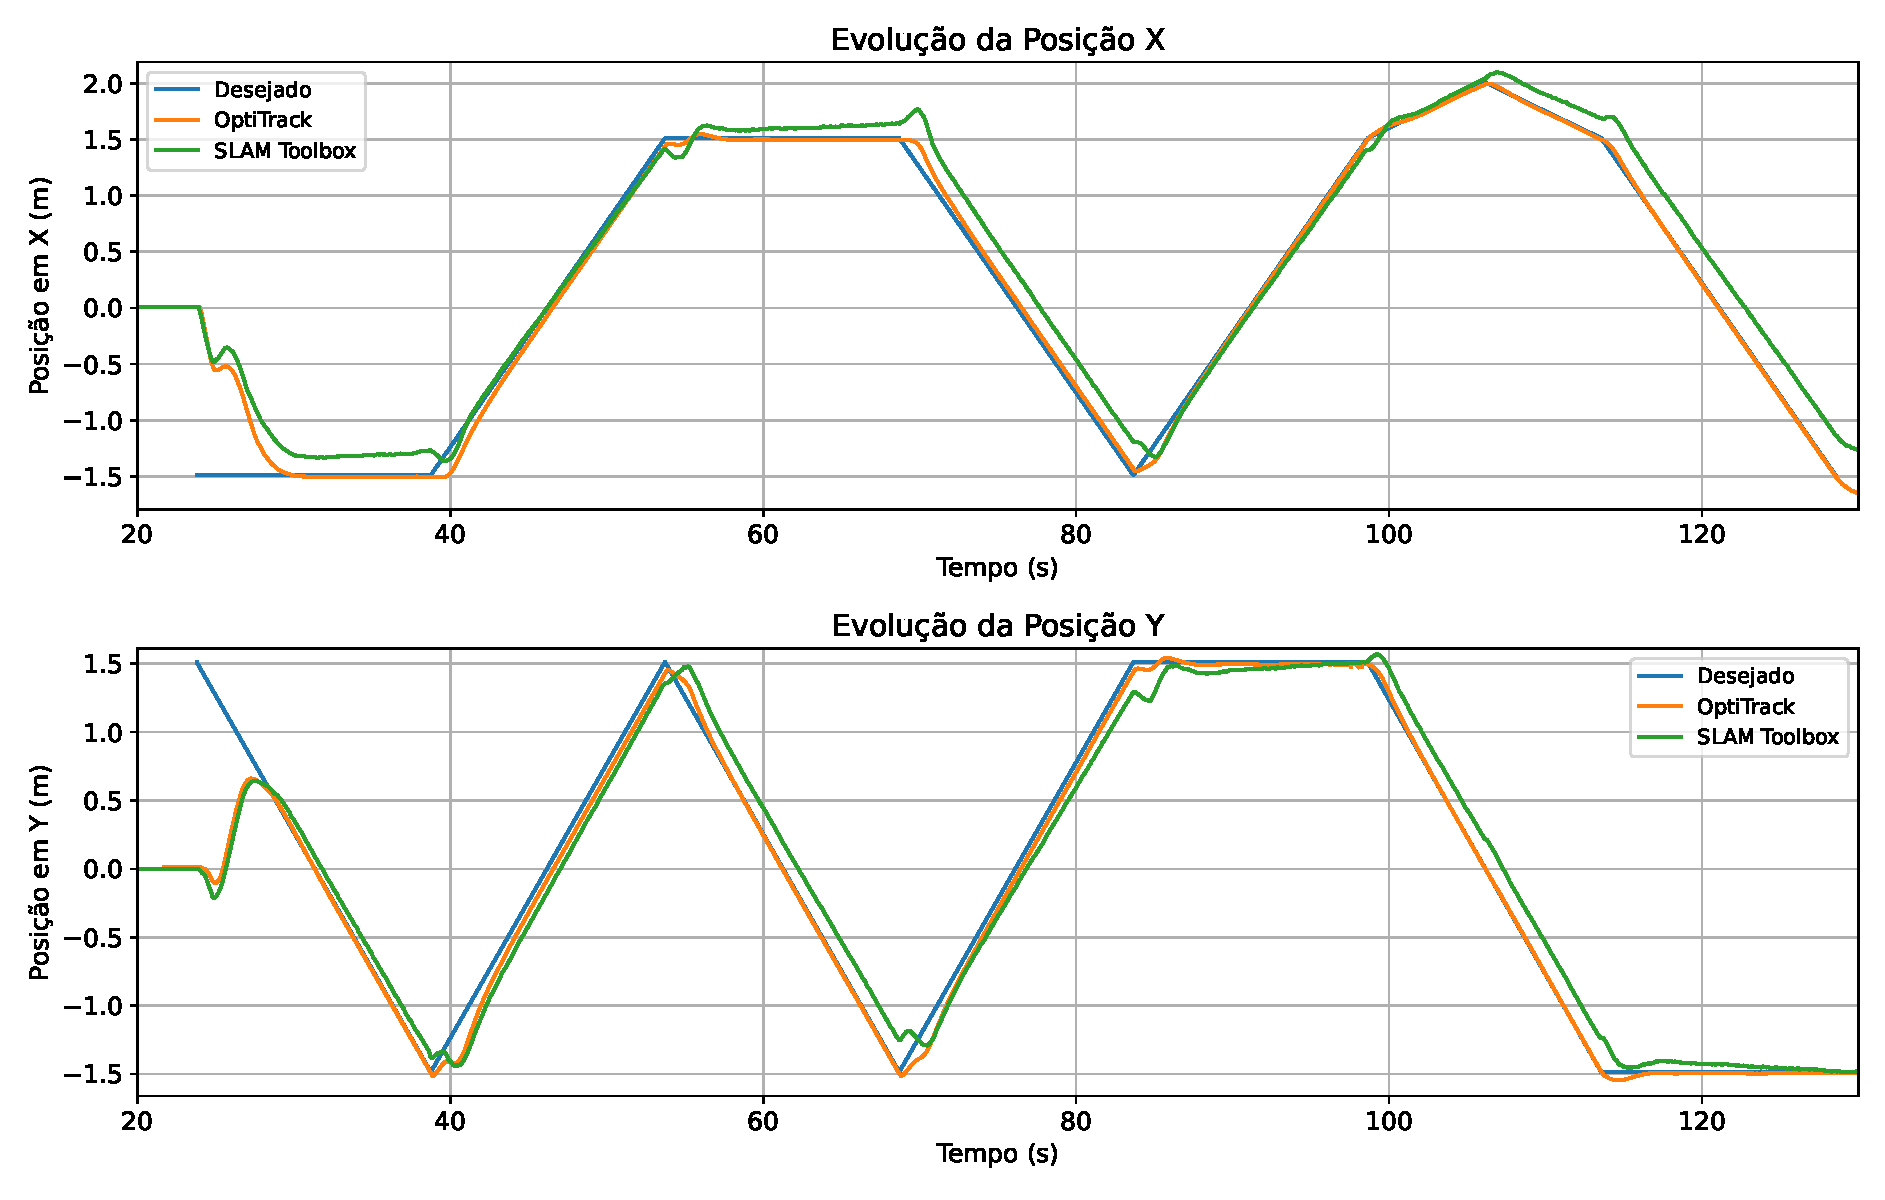
\includegraphics[width=\linewidth]{img/Resultados/Exp1_VRPN_Control_LINEAR/Exp1_pose_tempo.pdf}
    \sourceParbox[\linewidth]
    \label{fig:Exp1_XY_vs_tempo}
\end{figure}

% \begin{figure}[htb]
%     \centering
%     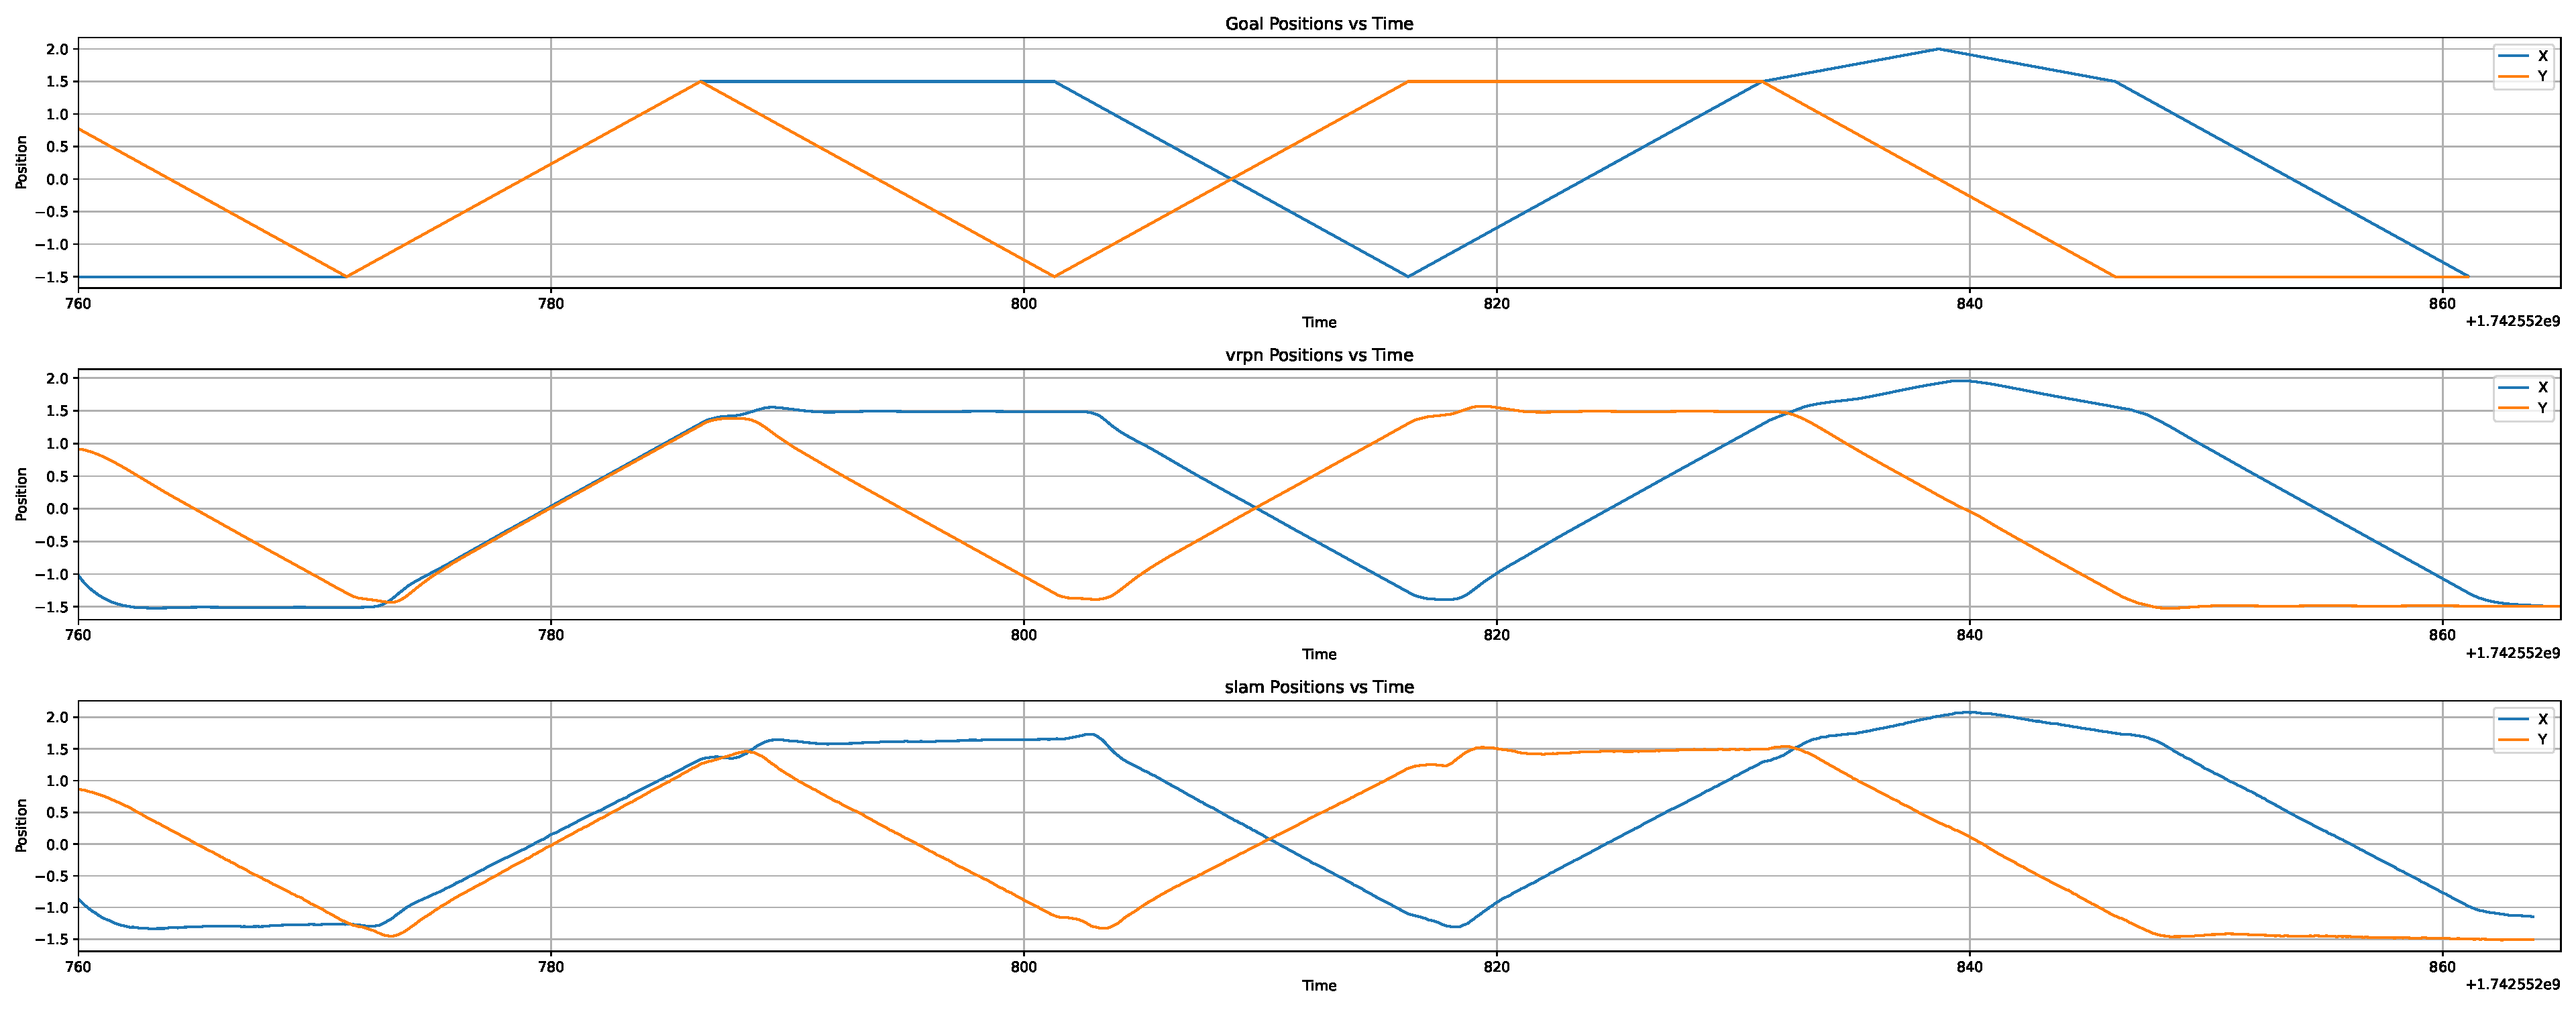
\includegraphics[width=1\linewidth]{img/Resultados/Exp1_VRPN_Control_LINEAR/Posicoes_v_tempo.pdf}
%     \caption{Enter Caption}
%     \label{fig:Exp1_Posicoes_Tempo}
% \end{figure}

% \begin{figure}[htb]
%     \centering
%     \caption{Experimento 1 - Erros de Posição}
%     \resizebox{\linewidth}{!}{
%     %% Creator: Matplotlib, PGF backend
%%
%% To include the figure in your LaTeX document, write
%%   \input{<filename>.pgf}
%%
%% Make sure the required packages are loaded in your preamble
%%   \usepackage{pgf}
%%
%% Also ensure that all the required font packages are loaded; for instance,
%% the lmodern package is sometimes necessary when using math font.
%%   \usepackage{lmodern}
%%
%% Figures using additional raster images can only be included by \input if
%% they are in the same directory as the main LaTeX file. For loading figures
%% from other directories you can use the `import` package
%%   \usepackage{import}
%%
%% and then include the figures with
%%   \import{<path to file>}{<filename>.pgf}
%%
%% Matplotlib used the following preamble
%%   
%%   \usepackage{fontspec}
%%   \setmainfont{DejaVuSerif.ttf}[Path=\detokenize{/home/maubp/.local/lib/python3.8/site-packages/matplotlib/mpl-data/fonts/ttf/}]
%%   \setsansfont{DejaVuSans.ttf}[Path=\detokenize{/home/maubp/.local/lib/python3.8/site-packages/matplotlib/mpl-data/fonts/ttf/}]
%%   \setmonofont{DejaVuSansMono.ttf}[Path=\detokenize{/home/maubp/.local/lib/python3.8/site-packages/matplotlib/mpl-data/fonts/ttf/}]
%%   \makeatletter\@ifpackageloaded{underscore}{}{\usepackage[strings]{underscore}}\makeatother
%%
\begingroup%
\makeatletter%
\begin{pgfpicture}%
\pgfpathrectangle{\pgfpointorigin}{\pgfqpoint{13.570000in}{9.770000in}}%
\pgfusepath{use as bounding box, clip}%
\begin{pgfscope}%
\pgfsetbuttcap%
\pgfsetmiterjoin%
\definecolor{currentfill}{rgb}{1.000000,1.000000,1.000000}%
\pgfsetfillcolor{currentfill}%
\pgfsetlinewidth{0.000000pt}%
\definecolor{currentstroke}{rgb}{1.000000,1.000000,1.000000}%
\pgfsetstrokecolor{currentstroke}%
\pgfsetdash{}{0pt}%
\pgfpathmoveto{\pgfqpoint{0.000000in}{0.000000in}}%
\pgfpathlineto{\pgfqpoint{13.570000in}{0.000000in}}%
\pgfpathlineto{\pgfqpoint{13.570000in}{9.770000in}}%
\pgfpathlineto{\pgfqpoint{0.000000in}{9.770000in}}%
\pgfpathlineto{\pgfqpoint{0.000000in}{0.000000in}}%
\pgfpathclose%
\pgfusepath{fill}%
\end{pgfscope}%
\begin{pgfscope}%
\pgfsetbuttcap%
\pgfsetmiterjoin%
\definecolor{currentfill}{rgb}{1.000000,1.000000,1.000000}%
\pgfsetfillcolor{currentfill}%
\pgfsetlinewidth{0.000000pt}%
\definecolor{currentstroke}{rgb}{0.000000,0.000000,0.000000}%
\pgfsetstrokecolor{currentstroke}%
\pgfsetstrokeopacity{0.000000}%
\pgfsetdash{}{0pt}%
\pgfpathmoveto{\pgfqpoint{1.021528in}{5.487778in}}%
\pgfpathlineto{\pgfqpoint{13.390000in}{5.487778in}}%
\pgfpathlineto{\pgfqpoint{13.390000in}{9.356667in}}%
\pgfpathlineto{\pgfqpoint{1.021528in}{9.356667in}}%
\pgfpathlineto{\pgfqpoint{1.021528in}{5.487778in}}%
\pgfpathclose%
\pgfusepath{fill}%
\end{pgfscope}%
\begin{pgfscope}%
\pgfpathrectangle{\pgfqpoint{1.021528in}{5.487778in}}{\pgfqpoint{12.368472in}{3.868889in}}%
\pgfusepath{clip}%
\pgfsetrectcap%
\pgfsetroundjoin%
\pgfsetlinewidth{0.803000pt}%
\definecolor{currentstroke}{rgb}{0.690196,0.690196,0.690196}%
\pgfsetstrokecolor{currentstroke}%
\pgfsetdash{}{0pt}%
\pgfpathmoveto{\pgfqpoint{1.021528in}{5.487778in}}%
\pgfpathlineto{\pgfqpoint{1.021528in}{9.356667in}}%
\pgfusepath{stroke}%
\end{pgfscope}%
\begin{pgfscope}%
\pgfsetbuttcap%
\pgfsetroundjoin%
\definecolor{currentfill}{rgb}{0.000000,0.000000,0.000000}%
\pgfsetfillcolor{currentfill}%
\pgfsetlinewidth{0.803000pt}%
\definecolor{currentstroke}{rgb}{0.000000,0.000000,0.000000}%
\pgfsetstrokecolor{currentstroke}%
\pgfsetdash{}{0pt}%
\pgfsys@defobject{currentmarker}{\pgfqpoint{0.000000in}{-0.048611in}}{\pgfqpoint{0.000000in}{0.000000in}}{%
\pgfpathmoveto{\pgfqpoint{0.000000in}{0.000000in}}%
\pgfpathlineto{\pgfqpoint{0.000000in}{-0.048611in}}%
\pgfusepath{stroke,fill}%
}%
\begin{pgfscope}%
\pgfsys@transformshift{1.021528in}{5.487778in}%
\pgfsys@useobject{currentmarker}{}%
\end{pgfscope}%
\end{pgfscope}%
\begin{pgfscope}%
\definecolor{textcolor}{rgb}{0.000000,0.000000,0.000000}%
\pgfsetstrokecolor{textcolor}%
\pgfsetfillcolor{textcolor}%
\pgftext[x=1.021528in,y=5.390556in,,top]{\color{textcolor}\sffamily\fontsize{12.000000}{14.400000}\selectfont 0}%
\end{pgfscope}%
\begin{pgfscope}%
\pgfpathrectangle{\pgfqpoint{1.021528in}{5.487778in}}{\pgfqpoint{12.368472in}{3.868889in}}%
\pgfusepath{clip}%
\pgfsetrectcap%
\pgfsetroundjoin%
\pgfsetlinewidth{0.803000pt}%
\definecolor{currentstroke}{rgb}{0.690196,0.690196,0.690196}%
\pgfsetstrokecolor{currentstroke}%
\pgfsetdash{}{0pt}%
\pgfpathmoveto{\pgfqpoint{3.209777in}{5.487778in}}%
\pgfpathlineto{\pgfqpoint{3.209777in}{9.356667in}}%
\pgfusepath{stroke}%
\end{pgfscope}%
\begin{pgfscope}%
\pgfsetbuttcap%
\pgfsetroundjoin%
\definecolor{currentfill}{rgb}{0.000000,0.000000,0.000000}%
\pgfsetfillcolor{currentfill}%
\pgfsetlinewidth{0.803000pt}%
\definecolor{currentstroke}{rgb}{0.000000,0.000000,0.000000}%
\pgfsetstrokecolor{currentstroke}%
\pgfsetdash{}{0pt}%
\pgfsys@defobject{currentmarker}{\pgfqpoint{0.000000in}{-0.048611in}}{\pgfqpoint{0.000000in}{0.000000in}}{%
\pgfpathmoveto{\pgfqpoint{0.000000in}{0.000000in}}%
\pgfpathlineto{\pgfqpoint{0.000000in}{-0.048611in}}%
\pgfusepath{stroke,fill}%
}%
\begin{pgfscope}%
\pgfsys@transformshift{3.209777in}{5.487778in}%
\pgfsys@useobject{currentmarker}{}%
\end{pgfscope}%
\end{pgfscope}%
\begin{pgfscope}%
\definecolor{textcolor}{rgb}{0.000000,0.000000,0.000000}%
\pgfsetstrokecolor{textcolor}%
\pgfsetfillcolor{textcolor}%
\pgftext[x=3.209777in,y=5.390556in,,top]{\color{textcolor}\sffamily\fontsize{12.000000}{14.400000}\selectfont 20}%
\end{pgfscope}%
\begin{pgfscope}%
\pgfpathrectangle{\pgfqpoint{1.021528in}{5.487778in}}{\pgfqpoint{12.368472in}{3.868889in}}%
\pgfusepath{clip}%
\pgfsetrectcap%
\pgfsetroundjoin%
\pgfsetlinewidth{0.803000pt}%
\definecolor{currentstroke}{rgb}{0.690196,0.690196,0.690196}%
\pgfsetstrokecolor{currentstroke}%
\pgfsetdash{}{0pt}%
\pgfpathmoveto{\pgfqpoint{5.398027in}{5.487778in}}%
\pgfpathlineto{\pgfqpoint{5.398027in}{9.356667in}}%
\pgfusepath{stroke}%
\end{pgfscope}%
\begin{pgfscope}%
\pgfsetbuttcap%
\pgfsetroundjoin%
\definecolor{currentfill}{rgb}{0.000000,0.000000,0.000000}%
\pgfsetfillcolor{currentfill}%
\pgfsetlinewidth{0.803000pt}%
\definecolor{currentstroke}{rgb}{0.000000,0.000000,0.000000}%
\pgfsetstrokecolor{currentstroke}%
\pgfsetdash{}{0pt}%
\pgfsys@defobject{currentmarker}{\pgfqpoint{0.000000in}{-0.048611in}}{\pgfqpoint{0.000000in}{0.000000in}}{%
\pgfpathmoveto{\pgfqpoint{0.000000in}{0.000000in}}%
\pgfpathlineto{\pgfqpoint{0.000000in}{-0.048611in}}%
\pgfusepath{stroke,fill}%
}%
\begin{pgfscope}%
\pgfsys@transformshift{5.398027in}{5.487778in}%
\pgfsys@useobject{currentmarker}{}%
\end{pgfscope}%
\end{pgfscope}%
\begin{pgfscope}%
\definecolor{textcolor}{rgb}{0.000000,0.000000,0.000000}%
\pgfsetstrokecolor{textcolor}%
\pgfsetfillcolor{textcolor}%
\pgftext[x=5.398027in,y=5.390556in,,top]{\color{textcolor}\sffamily\fontsize{12.000000}{14.400000}\selectfont 40}%
\end{pgfscope}%
\begin{pgfscope}%
\pgfpathrectangle{\pgfqpoint{1.021528in}{5.487778in}}{\pgfqpoint{12.368472in}{3.868889in}}%
\pgfusepath{clip}%
\pgfsetrectcap%
\pgfsetroundjoin%
\pgfsetlinewidth{0.803000pt}%
\definecolor{currentstroke}{rgb}{0.690196,0.690196,0.690196}%
\pgfsetstrokecolor{currentstroke}%
\pgfsetdash{}{0pt}%
\pgfpathmoveto{\pgfqpoint{7.586276in}{5.487778in}}%
\pgfpathlineto{\pgfqpoint{7.586276in}{9.356667in}}%
\pgfusepath{stroke}%
\end{pgfscope}%
\begin{pgfscope}%
\pgfsetbuttcap%
\pgfsetroundjoin%
\definecolor{currentfill}{rgb}{0.000000,0.000000,0.000000}%
\pgfsetfillcolor{currentfill}%
\pgfsetlinewidth{0.803000pt}%
\definecolor{currentstroke}{rgb}{0.000000,0.000000,0.000000}%
\pgfsetstrokecolor{currentstroke}%
\pgfsetdash{}{0pt}%
\pgfsys@defobject{currentmarker}{\pgfqpoint{0.000000in}{-0.048611in}}{\pgfqpoint{0.000000in}{0.000000in}}{%
\pgfpathmoveto{\pgfqpoint{0.000000in}{0.000000in}}%
\pgfpathlineto{\pgfqpoint{0.000000in}{-0.048611in}}%
\pgfusepath{stroke,fill}%
}%
\begin{pgfscope}%
\pgfsys@transformshift{7.586276in}{5.487778in}%
\pgfsys@useobject{currentmarker}{}%
\end{pgfscope}%
\end{pgfscope}%
\begin{pgfscope}%
\definecolor{textcolor}{rgb}{0.000000,0.000000,0.000000}%
\pgfsetstrokecolor{textcolor}%
\pgfsetfillcolor{textcolor}%
\pgftext[x=7.586276in,y=5.390556in,,top]{\color{textcolor}\sffamily\fontsize{12.000000}{14.400000}\selectfont 60}%
\end{pgfscope}%
\begin{pgfscope}%
\pgfpathrectangle{\pgfqpoint{1.021528in}{5.487778in}}{\pgfqpoint{12.368472in}{3.868889in}}%
\pgfusepath{clip}%
\pgfsetrectcap%
\pgfsetroundjoin%
\pgfsetlinewidth{0.803000pt}%
\definecolor{currentstroke}{rgb}{0.690196,0.690196,0.690196}%
\pgfsetstrokecolor{currentstroke}%
\pgfsetdash{}{0pt}%
\pgfpathmoveto{\pgfqpoint{9.774526in}{5.487778in}}%
\pgfpathlineto{\pgfqpoint{9.774526in}{9.356667in}}%
\pgfusepath{stroke}%
\end{pgfscope}%
\begin{pgfscope}%
\pgfsetbuttcap%
\pgfsetroundjoin%
\definecolor{currentfill}{rgb}{0.000000,0.000000,0.000000}%
\pgfsetfillcolor{currentfill}%
\pgfsetlinewidth{0.803000pt}%
\definecolor{currentstroke}{rgb}{0.000000,0.000000,0.000000}%
\pgfsetstrokecolor{currentstroke}%
\pgfsetdash{}{0pt}%
\pgfsys@defobject{currentmarker}{\pgfqpoint{0.000000in}{-0.048611in}}{\pgfqpoint{0.000000in}{0.000000in}}{%
\pgfpathmoveto{\pgfqpoint{0.000000in}{0.000000in}}%
\pgfpathlineto{\pgfqpoint{0.000000in}{-0.048611in}}%
\pgfusepath{stroke,fill}%
}%
\begin{pgfscope}%
\pgfsys@transformshift{9.774526in}{5.487778in}%
\pgfsys@useobject{currentmarker}{}%
\end{pgfscope}%
\end{pgfscope}%
\begin{pgfscope}%
\definecolor{textcolor}{rgb}{0.000000,0.000000,0.000000}%
\pgfsetstrokecolor{textcolor}%
\pgfsetfillcolor{textcolor}%
\pgftext[x=9.774526in,y=5.390556in,,top]{\color{textcolor}\sffamily\fontsize{12.000000}{14.400000}\selectfont 80}%
\end{pgfscope}%
\begin{pgfscope}%
\pgfpathrectangle{\pgfqpoint{1.021528in}{5.487778in}}{\pgfqpoint{12.368472in}{3.868889in}}%
\pgfusepath{clip}%
\pgfsetrectcap%
\pgfsetroundjoin%
\pgfsetlinewidth{0.803000pt}%
\definecolor{currentstroke}{rgb}{0.690196,0.690196,0.690196}%
\pgfsetstrokecolor{currentstroke}%
\pgfsetdash{}{0pt}%
\pgfpathmoveto{\pgfqpoint{11.962775in}{5.487778in}}%
\pgfpathlineto{\pgfqpoint{11.962775in}{9.356667in}}%
\pgfusepath{stroke}%
\end{pgfscope}%
\begin{pgfscope}%
\pgfsetbuttcap%
\pgfsetroundjoin%
\definecolor{currentfill}{rgb}{0.000000,0.000000,0.000000}%
\pgfsetfillcolor{currentfill}%
\pgfsetlinewidth{0.803000pt}%
\definecolor{currentstroke}{rgb}{0.000000,0.000000,0.000000}%
\pgfsetstrokecolor{currentstroke}%
\pgfsetdash{}{0pt}%
\pgfsys@defobject{currentmarker}{\pgfqpoint{0.000000in}{-0.048611in}}{\pgfqpoint{0.000000in}{0.000000in}}{%
\pgfpathmoveto{\pgfqpoint{0.000000in}{0.000000in}}%
\pgfpathlineto{\pgfqpoint{0.000000in}{-0.048611in}}%
\pgfusepath{stroke,fill}%
}%
\begin{pgfscope}%
\pgfsys@transformshift{11.962775in}{5.487778in}%
\pgfsys@useobject{currentmarker}{}%
\end{pgfscope}%
\end{pgfscope}%
\begin{pgfscope}%
\definecolor{textcolor}{rgb}{0.000000,0.000000,0.000000}%
\pgfsetstrokecolor{textcolor}%
\pgfsetfillcolor{textcolor}%
\pgftext[x=11.962775in,y=5.390556in,,top]{\color{textcolor}\sffamily\fontsize{12.000000}{14.400000}\selectfont 100}%
\end{pgfscope}%
\begin{pgfscope}%
\definecolor{textcolor}{rgb}{0.000000,0.000000,0.000000}%
\pgfsetstrokecolor{textcolor}%
\pgfsetfillcolor{textcolor}%
\pgftext[x=7.205764in,y=5.173705in,,top]{\color{textcolor}\sffamily\fontsize{12.000000}{14.400000}\selectfont Time (s)}%
\end{pgfscope}%
\begin{pgfscope}%
\pgfpathrectangle{\pgfqpoint{1.021528in}{5.487778in}}{\pgfqpoint{12.368472in}{3.868889in}}%
\pgfusepath{clip}%
\pgfsetrectcap%
\pgfsetroundjoin%
\pgfsetlinewidth{0.803000pt}%
\definecolor{currentstroke}{rgb}{0.690196,0.690196,0.690196}%
\pgfsetstrokecolor{currentstroke}%
\pgfsetdash{}{0pt}%
\pgfpathmoveto{\pgfqpoint{1.021528in}{5.793623in}}%
\pgfpathlineto{\pgfqpoint{13.390000in}{5.793623in}}%
\pgfusepath{stroke}%
\end{pgfscope}%
\begin{pgfscope}%
\pgfsetbuttcap%
\pgfsetroundjoin%
\definecolor{currentfill}{rgb}{0.000000,0.000000,0.000000}%
\pgfsetfillcolor{currentfill}%
\pgfsetlinewidth{0.803000pt}%
\definecolor{currentstroke}{rgb}{0.000000,0.000000,0.000000}%
\pgfsetstrokecolor{currentstroke}%
\pgfsetdash{}{0pt}%
\pgfsys@defobject{currentmarker}{\pgfqpoint{-0.048611in}{0.000000in}}{\pgfqpoint{-0.000000in}{0.000000in}}{%
\pgfpathmoveto{\pgfqpoint{-0.000000in}{0.000000in}}%
\pgfpathlineto{\pgfqpoint{-0.048611in}{0.000000in}}%
\pgfusepath{stroke,fill}%
}%
\begin{pgfscope}%
\pgfsys@transformshift{1.021528in}{5.793623in}%
\pgfsys@useobject{currentmarker}{}%
\end{pgfscope}%
\end{pgfscope}%
\begin{pgfscope}%
\definecolor{textcolor}{rgb}{0.000000,0.000000,0.000000}%
\pgfsetstrokecolor{textcolor}%
\pgfsetfillcolor{textcolor}%
\pgftext[x=0.423582in, y=5.730310in, left, base]{\color{textcolor}\sffamily\fontsize{12.000000}{14.400000}\selectfont \ensuremath{-}0.25}%
\end{pgfscope}%
\begin{pgfscope}%
\pgfpathrectangle{\pgfqpoint{1.021528in}{5.487778in}}{\pgfqpoint{12.368472in}{3.868889in}}%
\pgfusepath{clip}%
\pgfsetrectcap%
\pgfsetroundjoin%
\pgfsetlinewidth{0.803000pt}%
\definecolor{currentstroke}{rgb}{0.690196,0.690196,0.690196}%
\pgfsetstrokecolor{currentstroke}%
\pgfsetdash{}{0pt}%
\pgfpathmoveto{\pgfqpoint{1.021528in}{6.296516in}}%
\pgfpathlineto{\pgfqpoint{13.390000in}{6.296516in}}%
\pgfusepath{stroke}%
\end{pgfscope}%
\begin{pgfscope}%
\pgfsetbuttcap%
\pgfsetroundjoin%
\definecolor{currentfill}{rgb}{0.000000,0.000000,0.000000}%
\pgfsetfillcolor{currentfill}%
\pgfsetlinewidth{0.803000pt}%
\definecolor{currentstroke}{rgb}{0.000000,0.000000,0.000000}%
\pgfsetstrokecolor{currentstroke}%
\pgfsetdash{}{0pt}%
\pgfsys@defobject{currentmarker}{\pgfqpoint{-0.048611in}{0.000000in}}{\pgfqpoint{-0.000000in}{0.000000in}}{%
\pgfpathmoveto{\pgfqpoint{-0.000000in}{0.000000in}}%
\pgfpathlineto{\pgfqpoint{-0.048611in}{0.000000in}}%
\pgfusepath{stroke,fill}%
}%
\begin{pgfscope}%
\pgfsys@transformshift{1.021528in}{6.296516in}%
\pgfsys@useobject{currentmarker}{}%
\end{pgfscope}%
\end{pgfscope}%
\begin{pgfscope}%
\definecolor{textcolor}{rgb}{0.000000,0.000000,0.000000}%
\pgfsetstrokecolor{textcolor}%
\pgfsetfillcolor{textcolor}%
\pgftext[x=0.553212in, y=6.233202in, left, base]{\color{textcolor}\sffamily\fontsize{12.000000}{14.400000}\selectfont 0.00}%
\end{pgfscope}%
\begin{pgfscope}%
\pgfpathrectangle{\pgfqpoint{1.021528in}{5.487778in}}{\pgfqpoint{12.368472in}{3.868889in}}%
\pgfusepath{clip}%
\pgfsetrectcap%
\pgfsetroundjoin%
\pgfsetlinewidth{0.803000pt}%
\definecolor{currentstroke}{rgb}{0.690196,0.690196,0.690196}%
\pgfsetstrokecolor{currentstroke}%
\pgfsetdash{}{0pt}%
\pgfpathmoveto{\pgfqpoint{1.021528in}{6.799409in}}%
\pgfpathlineto{\pgfqpoint{13.390000in}{6.799409in}}%
\pgfusepath{stroke}%
\end{pgfscope}%
\begin{pgfscope}%
\pgfsetbuttcap%
\pgfsetroundjoin%
\definecolor{currentfill}{rgb}{0.000000,0.000000,0.000000}%
\pgfsetfillcolor{currentfill}%
\pgfsetlinewidth{0.803000pt}%
\definecolor{currentstroke}{rgb}{0.000000,0.000000,0.000000}%
\pgfsetstrokecolor{currentstroke}%
\pgfsetdash{}{0pt}%
\pgfsys@defobject{currentmarker}{\pgfqpoint{-0.048611in}{0.000000in}}{\pgfqpoint{-0.000000in}{0.000000in}}{%
\pgfpathmoveto{\pgfqpoint{-0.000000in}{0.000000in}}%
\pgfpathlineto{\pgfqpoint{-0.048611in}{0.000000in}}%
\pgfusepath{stroke,fill}%
}%
\begin{pgfscope}%
\pgfsys@transformshift{1.021528in}{6.799409in}%
\pgfsys@useobject{currentmarker}{}%
\end{pgfscope}%
\end{pgfscope}%
\begin{pgfscope}%
\definecolor{textcolor}{rgb}{0.000000,0.000000,0.000000}%
\pgfsetstrokecolor{textcolor}%
\pgfsetfillcolor{textcolor}%
\pgftext[x=0.553212in, y=6.736095in, left, base]{\color{textcolor}\sffamily\fontsize{12.000000}{14.400000}\selectfont 0.25}%
\end{pgfscope}%
\begin{pgfscope}%
\pgfpathrectangle{\pgfqpoint{1.021528in}{5.487778in}}{\pgfqpoint{12.368472in}{3.868889in}}%
\pgfusepath{clip}%
\pgfsetrectcap%
\pgfsetroundjoin%
\pgfsetlinewidth{0.803000pt}%
\definecolor{currentstroke}{rgb}{0.690196,0.690196,0.690196}%
\pgfsetstrokecolor{currentstroke}%
\pgfsetdash{}{0pt}%
\pgfpathmoveto{\pgfqpoint{1.021528in}{7.302301in}}%
\pgfpathlineto{\pgfqpoint{13.390000in}{7.302301in}}%
\pgfusepath{stroke}%
\end{pgfscope}%
\begin{pgfscope}%
\pgfsetbuttcap%
\pgfsetroundjoin%
\definecolor{currentfill}{rgb}{0.000000,0.000000,0.000000}%
\pgfsetfillcolor{currentfill}%
\pgfsetlinewidth{0.803000pt}%
\definecolor{currentstroke}{rgb}{0.000000,0.000000,0.000000}%
\pgfsetstrokecolor{currentstroke}%
\pgfsetdash{}{0pt}%
\pgfsys@defobject{currentmarker}{\pgfqpoint{-0.048611in}{0.000000in}}{\pgfqpoint{-0.000000in}{0.000000in}}{%
\pgfpathmoveto{\pgfqpoint{-0.000000in}{0.000000in}}%
\pgfpathlineto{\pgfqpoint{-0.048611in}{0.000000in}}%
\pgfusepath{stroke,fill}%
}%
\begin{pgfscope}%
\pgfsys@transformshift{1.021528in}{7.302301in}%
\pgfsys@useobject{currentmarker}{}%
\end{pgfscope}%
\end{pgfscope}%
\begin{pgfscope}%
\definecolor{textcolor}{rgb}{0.000000,0.000000,0.000000}%
\pgfsetstrokecolor{textcolor}%
\pgfsetfillcolor{textcolor}%
\pgftext[x=0.553212in, y=7.238988in, left, base]{\color{textcolor}\sffamily\fontsize{12.000000}{14.400000}\selectfont 0.50}%
\end{pgfscope}%
\begin{pgfscope}%
\pgfpathrectangle{\pgfqpoint{1.021528in}{5.487778in}}{\pgfqpoint{12.368472in}{3.868889in}}%
\pgfusepath{clip}%
\pgfsetrectcap%
\pgfsetroundjoin%
\pgfsetlinewidth{0.803000pt}%
\definecolor{currentstroke}{rgb}{0.690196,0.690196,0.690196}%
\pgfsetstrokecolor{currentstroke}%
\pgfsetdash{}{0pt}%
\pgfpathmoveto{\pgfqpoint{1.021528in}{7.805194in}}%
\pgfpathlineto{\pgfqpoint{13.390000in}{7.805194in}}%
\pgfusepath{stroke}%
\end{pgfscope}%
\begin{pgfscope}%
\pgfsetbuttcap%
\pgfsetroundjoin%
\definecolor{currentfill}{rgb}{0.000000,0.000000,0.000000}%
\pgfsetfillcolor{currentfill}%
\pgfsetlinewidth{0.803000pt}%
\definecolor{currentstroke}{rgb}{0.000000,0.000000,0.000000}%
\pgfsetstrokecolor{currentstroke}%
\pgfsetdash{}{0pt}%
\pgfsys@defobject{currentmarker}{\pgfqpoint{-0.048611in}{0.000000in}}{\pgfqpoint{-0.000000in}{0.000000in}}{%
\pgfpathmoveto{\pgfqpoint{-0.000000in}{0.000000in}}%
\pgfpathlineto{\pgfqpoint{-0.048611in}{0.000000in}}%
\pgfusepath{stroke,fill}%
}%
\begin{pgfscope}%
\pgfsys@transformshift{1.021528in}{7.805194in}%
\pgfsys@useobject{currentmarker}{}%
\end{pgfscope}%
\end{pgfscope}%
\begin{pgfscope}%
\definecolor{textcolor}{rgb}{0.000000,0.000000,0.000000}%
\pgfsetstrokecolor{textcolor}%
\pgfsetfillcolor{textcolor}%
\pgftext[x=0.553212in, y=7.741880in, left, base]{\color{textcolor}\sffamily\fontsize{12.000000}{14.400000}\selectfont 0.75}%
\end{pgfscope}%
\begin{pgfscope}%
\pgfpathrectangle{\pgfqpoint{1.021528in}{5.487778in}}{\pgfqpoint{12.368472in}{3.868889in}}%
\pgfusepath{clip}%
\pgfsetrectcap%
\pgfsetroundjoin%
\pgfsetlinewidth{0.803000pt}%
\definecolor{currentstroke}{rgb}{0.690196,0.690196,0.690196}%
\pgfsetstrokecolor{currentstroke}%
\pgfsetdash{}{0pt}%
\pgfpathmoveto{\pgfqpoint{1.021528in}{8.308087in}}%
\pgfpathlineto{\pgfqpoint{13.390000in}{8.308087in}}%
\pgfusepath{stroke}%
\end{pgfscope}%
\begin{pgfscope}%
\pgfsetbuttcap%
\pgfsetroundjoin%
\definecolor{currentfill}{rgb}{0.000000,0.000000,0.000000}%
\pgfsetfillcolor{currentfill}%
\pgfsetlinewidth{0.803000pt}%
\definecolor{currentstroke}{rgb}{0.000000,0.000000,0.000000}%
\pgfsetstrokecolor{currentstroke}%
\pgfsetdash{}{0pt}%
\pgfsys@defobject{currentmarker}{\pgfqpoint{-0.048611in}{0.000000in}}{\pgfqpoint{-0.000000in}{0.000000in}}{%
\pgfpathmoveto{\pgfqpoint{-0.000000in}{0.000000in}}%
\pgfpathlineto{\pgfqpoint{-0.048611in}{0.000000in}}%
\pgfusepath{stroke,fill}%
}%
\begin{pgfscope}%
\pgfsys@transformshift{1.021528in}{8.308087in}%
\pgfsys@useobject{currentmarker}{}%
\end{pgfscope}%
\end{pgfscope}%
\begin{pgfscope}%
\definecolor{textcolor}{rgb}{0.000000,0.000000,0.000000}%
\pgfsetstrokecolor{textcolor}%
\pgfsetfillcolor{textcolor}%
\pgftext[x=0.553212in, y=8.244773in, left, base]{\color{textcolor}\sffamily\fontsize{12.000000}{14.400000}\selectfont 1.00}%
\end{pgfscope}%
\begin{pgfscope}%
\pgfpathrectangle{\pgfqpoint{1.021528in}{5.487778in}}{\pgfqpoint{12.368472in}{3.868889in}}%
\pgfusepath{clip}%
\pgfsetrectcap%
\pgfsetroundjoin%
\pgfsetlinewidth{0.803000pt}%
\definecolor{currentstroke}{rgb}{0.690196,0.690196,0.690196}%
\pgfsetstrokecolor{currentstroke}%
\pgfsetdash{}{0pt}%
\pgfpathmoveto{\pgfqpoint{1.021528in}{8.810979in}}%
\pgfpathlineto{\pgfqpoint{13.390000in}{8.810979in}}%
\pgfusepath{stroke}%
\end{pgfscope}%
\begin{pgfscope}%
\pgfsetbuttcap%
\pgfsetroundjoin%
\definecolor{currentfill}{rgb}{0.000000,0.000000,0.000000}%
\pgfsetfillcolor{currentfill}%
\pgfsetlinewidth{0.803000pt}%
\definecolor{currentstroke}{rgb}{0.000000,0.000000,0.000000}%
\pgfsetstrokecolor{currentstroke}%
\pgfsetdash{}{0pt}%
\pgfsys@defobject{currentmarker}{\pgfqpoint{-0.048611in}{0.000000in}}{\pgfqpoint{-0.000000in}{0.000000in}}{%
\pgfpathmoveto{\pgfqpoint{-0.000000in}{0.000000in}}%
\pgfpathlineto{\pgfqpoint{-0.048611in}{0.000000in}}%
\pgfusepath{stroke,fill}%
}%
\begin{pgfscope}%
\pgfsys@transformshift{1.021528in}{8.810979in}%
\pgfsys@useobject{currentmarker}{}%
\end{pgfscope}%
\end{pgfscope}%
\begin{pgfscope}%
\definecolor{textcolor}{rgb}{0.000000,0.000000,0.000000}%
\pgfsetstrokecolor{textcolor}%
\pgfsetfillcolor{textcolor}%
\pgftext[x=0.553212in, y=8.747666in, left, base]{\color{textcolor}\sffamily\fontsize{12.000000}{14.400000}\selectfont 1.25}%
\end{pgfscope}%
\begin{pgfscope}%
\pgfpathrectangle{\pgfqpoint{1.021528in}{5.487778in}}{\pgfqpoint{12.368472in}{3.868889in}}%
\pgfusepath{clip}%
\pgfsetrectcap%
\pgfsetroundjoin%
\pgfsetlinewidth{0.803000pt}%
\definecolor{currentstroke}{rgb}{0.690196,0.690196,0.690196}%
\pgfsetstrokecolor{currentstroke}%
\pgfsetdash{}{0pt}%
\pgfpathmoveto{\pgfqpoint{1.021528in}{9.313872in}}%
\pgfpathlineto{\pgfqpoint{13.390000in}{9.313872in}}%
\pgfusepath{stroke}%
\end{pgfscope}%
\begin{pgfscope}%
\pgfsetbuttcap%
\pgfsetroundjoin%
\definecolor{currentfill}{rgb}{0.000000,0.000000,0.000000}%
\pgfsetfillcolor{currentfill}%
\pgfsetlinewidth{0.803000pt}%
\definecolor{currentstroke}{rgb}{0.000000,0.000000,0.000000}%
\pgfsetstrokecolor{currentstroke}%
\pgfsetdash{}{0pt}%
\pgfsys@defobject{currentmarker}{\pgfqpoint{-0.048611in}{0.000000in}}{\pgfqpoint{-0.000000in}{0.000000in}}{%
\pgfpathmoveto{\pgfqpoint{-0.000000in}{0.000000in}}%
\pgfpathlineto{\pgfqpoint{-0.048611in}{0.000000in}}%
\pgfusepath{stroke,fill}%
}%
\begin{pgfscope}%
\pgfsys@transformshift{1.021528in}{9.313872in}%
\pgfsys@useobject{currentmarker}{}%
\end{pgfscope}%
\end{pgfscope}%
\begin{pgfscope}%
\definecolor{textcolor}{rgb}{0.000000,0.000000,0.000000}%
\pgfsetstrokecolor{textcolor}%
\pgfsetfillcolor{textcolor}%
\pgftext[x=0.553212in, y=9.250558in, left, base]{\color{textcolor}\sffamily\fontsize{12.000000}{14.400000}\selectfont 1.50}%
\end{pgfscope}%
\begin{pgfscope}%
\definecolor{textcolor}{rgb}{0.000000,0.000000,0.000000}%
\pgfsetstrokecolor{textcolor}%
\pgfsetfillcolor{textcolor}%
\pgftext[x=0.368026in,y=7.422222in,,bottom,rotate=90.000000]{\color{textcolor}\sffamily\fontsize{12.000000}{14.400000}\selectfont X Error}%
\end{pgfscope}%
\begin{pgfscope}%
\pgfpathrectangle{\pgfqpoint{1.021528in}{5.487778in}}{\pgfqpoint{12.368472in}{3.868889in}}%
\pgfusepath{clip}%
\pgfsetrectcap%
\pgfsetroundjoin%
\pgfsetlinewidth{1.505625pt}%
\definecolor{currentstroke}{rgb}{0.121569,0.466667,0.705882}%
\pgfsetstrokecolor{currentstroke}%
\pgfsetdash{}{0pt}%
\pgfpathmoveto{\pgfqpoint{1.021528in}{9.179995in}}%
\pgfpathlineto{\pgfqpoint{1.030646in}{9.179976in}}%
\pgfpathlineto{\pgfqpoint{1.039763in}{9.179920in}}%
\pgfpathlineto{\pgfqpoint{1.059214in}{9.180027in}}%
\pgfpathlineto{\pgfqpoint{1.066508in}{9.179954in}}%
\pgfpathlineto{\pgfqpoint{1.084136in}{9.180035in}}%
\pgfpathlineto{\pgfqpoint{1.090215in}{9.179987in}}%
\pgfpathlineto{\pgfqpoint{1.126078in}{9.180007in}}%
\pgfpathlineto{\pgfqpoint{1.137019in}{9.180060in}}%
\pgfpathlineto{\pgfqpoint{1.144921in}{9.179974in}}%
\pgfpathlineto{\pgfqpoint{1.174705in}{9.180125in}}%
\pgfpathlineto{\pgfqpoint{1.259804in}{9.180153in}}%
\pgfpathlineto{\pgfqpoint{1.268314in}{9.180198in}}%
\pgfpathlineto{\pgfqpoint{1.273784in}{9.180069in}}%
\pgfpathlineto{\pgfqpoint{1.361922in}{9.179158in}}%
\pgfpathlineto{\pgfqpoint{1.364354in}{9.175367in}}%
\pgfpathlineto{\pgfqpoint{1.368001in}{9.163900in}}%
\pgfpathlineto{\pgfqpoint{1.371040in}{9.149070in}}%
\pgfpathlineto{\pgfqpoint{1.375903in}{9.112063in}}%
\pgfpathlineto{\pgfqpoint{1.382589in}{9.032536in}}%
\pgfpathlineto{\pgfqpoint{1.422099in}{8.528233in}}%
\pgfpathlineto{\pgfqpoint{1.439119in}{8.355815in}}%
\pgfpathlineto{\pgfqpoint{1.446413in}{8.309976in}}%
\pgfpathlineto{\pgfqpoint{1.453707in}{8.284525in}}%
\pgfpathlineto{\pgfqpoint{1.459786in}{8.275302in}}%
\pgfpathlineto{\pgfqpoint{1.463433in}{8.273093in}}%
\pgfpathlineto{\pgfqpoint{1.468295in}{8.273743in}}%
\pgfpathlineto{\pgfqpoint{1.471942in}{8.276117in}}%
\pgfpathlineto{\pgfqpoint{1.484707in}{8.295176in}}%
\pgfpathlineto{\pgfqpoint{1.497472in}{8.323103in}}%
\pgfpathlineto{\pgfqpoint{1.527864in}{8.420226in}}%
\pgfpathlineto{\pgfqpoint{1.530904in}{8.428005in}}%
\pgfpathlineto{\pgfqpoint{1.535766in}{8.440247in}}%
\pgfpathlineto{\pgfqpoint{1.541237in}{8.451136in}}%
\pgfpathlineto{\pgfqpoint{1.543061in}{8.453598in}}%
\pgfpathlineto{\pgfqpoint{1.552178in}{8.464559in}}%
\pgfpathlineto{\pgfqpoint{1.553394in}{8.465408in}}%
\pgfpathlineto{\pgfqpoint{1.560080in}{8.467846in}}%
\pgfpathlineto{\pgfqpoint{1.562512in}{8.467206in}}%
\pgfpathlineto{\pgfqpoint{1.565551in}{8.466816in}}%
\pgfpathlineto{\pgfqpoint{1.571629in}{8.462807in}}%
\pgfpathlineto{\pgfqpoint{1.575276in}{8.459280in}}%
\pgfpathlineto{\pgfqpoint{1.579531in}{8.453457in}}%
\pgfpathlineto{\pgfqpoint{1.586826in}{8.441285in}}%
\pgfpathlineto{\pgfqpoint{1.592904in}{8.426771in}}%
\pgfpathlineto{\pgfqpoint{1.597159in}{8.415704in}}%
\pgfpathlineto{\pgfqpoint{1.603845in}{8.393434in}}%
\pgfpathlineto{\pgfqpoint{1.619041in}{8.320685in}}%
\pgfpathlineto{\pgfqpoint{1.631806in}{8.245501in}}%
\pgfpathlineto{\pgfqpoint{1.643355in}{8.161819in}}%
\pgfpathlineto{\pgfqpoint{1.662199in}{8.011020in}}%
\pgfpathlineto{\pgfqpoint{1.675571in}{7.899114in}}%
\pgfpathlineto{\pgfqpoint{1.692591in}{7.742586in}}%
\pgfpathlineto{\pgfqpoint{1.711434in}{7.559650in}}%
\pgfpathlineto{\pgfqpoint{1.759454in}{7.107099in}}%
\pgfpathlineto{\pgfqpoint{1.789239in}{6.895964in}}%
\pgfpathlineto{\pgfqpoint{1.794709in}{6.863316in}}%
\pgfpathlineto{\pgfqpoint{1.814768in}{6.753002in}}%
\pgfpathlineto{\pgfqpoint{1.838474in}{6.642989in}}%
\pgfpathlineto{\pgfqpoint{1.876769in}{6.498779in}}%
\pgfpathlineto{\pgfqpoint{1.884671in}{6.473997in}}%
\pgfpathlineto{\pgfqpoint{1.895612in}{6.442838in}}%
\pgfpathlineto{\pgfqpoint{1.920534in}{6.383939in}}%
\pgfpathlineto{\pgfqpoint{1.933906in}{6.357426in}}%
\pgfpathlineto{\pgfqpoint{1.938769in}{6.348897in}}%
\pgfpathlineto{\pgfqpoint{1.944847in}{6.340227in}}%
\pgfpathlineto{\pgfqpoint{1.948495in}{6.333609in}}%
\pgfpathlineto{\pgfqpoint{1.952749in}{6.327454in}}%
\pgfpathlineto{\pgfqpoint{1.955789in}{6.323210in}}%
\pgfpathlineto{\pgfqpoint{1.961259in}{6.316169in}}%
\pgfpathlineto{\pgfqpoint{1.966122in}{6.309330in}}%
\pgfpathlineto{\pgfqpoint{1.969769in}{6.306252in}}%
\pgfpathlineto{\pgfqpoint{1.974632in}{6.299936in}}%
\pgfpathlineto{\pgfqpoint{1.977063in}{6.298246in}}%
\pgfpathlineto{\pgfqpoint{1.979495in}{6.294967in}}%
\pgfpathlineto{\pgfqpoint{1.982534in}{6.291688in}}%
\pgfpathlineto{\pgfqpoint{1.991044in}{6.284447in}}%
\pgfpathlineto{\pgfqpoint{1.994083in}{6.282294in}}%
\pgfpathlineto{\pgfqpoint{1.998946in}{6.279056in}}%
\pgfpathlineto{\pgfqpoint{2.000769in}{6.277909in}}%
\pgfpathlineto{\pgfqpoint{2.006848in}{6.274087in}}%
\pgfpathlineto{\pgfqpoint{2.009887in}{6.272176in}}%
\pgfpathlineto{\pgfqpoint{2.012319in}{6.270527in}}%
\pgfpathlineto{\pgfqpoint{2.014750in}{6.269440in}}%
\pgfpathlineto{\pgfqpoint{2.019005in}{6.267389in}}%
\pgfpathlineto{\pgfqpoint{2.045750in}{6.258558in}}%
\pgfpathlineto{\pgfqpoint{2.046966in}{6.258357in}}%
\pgfpathlineto{\pgfqpoint{2.050613in}{6.258055in}}%
\pgfpathlineto{\pgfqpoint{2.051221in}{6.258055in}}%
\pgfpathlineto{\pgfqpoint{2.052436in}{6.256848in}}%
\pgfpathlineto{\pgfqpoint{2.054260in}{6.256486in}}%
\pgfpathlineto{\pgfqpoint{2.059731in}{6.255500in}}%
\pgfpathlineto{\pgfqpoint{2.067025in}{6.254273in}}%
\pgfpathlineto{\pgfqpoint{2.070064in}{6.254313in}}%
\pgfpathlineto{\pgfqpoint{2.072495in}{6.253971in}}%
\pgfpathlineto{\pgfqpoint{2.075535in}{6.253851in}}%
\pgfpathlineto{\pgfqpoint{2.077358in}{6.253649in}}%
\pgfpathlineto{\pgfqpoint{2.081613in}{6.253569in}}%
\pgfpathlineto{\pgfqpoint{2.082829in}{6.254354in}}%
\pgfpathlineto{\pgfqpoint{2.083437in}{6.254394in}}%
\pgfpathlineto{\pgfqpoint{2.084044in}{6.252945in}}%
\pgfpathlineto{\pgfqpoint{2.084652in}{6.254112in}}%
\pgfpathlineto{\pgfqpoint{2.096809in}{6.254354in}}%
\pgfpathlineto{\pgfqpoint{2.098633in}{6.254595in}}%
\pgfpathlineto{\pgfqpoint{2.105319in}{6.254313in}}%
\pgfpathlineto{\pgfqpoint{2.129633in}{6.256707in}}%
\pgfpathlineto{\pgfqpoint{2.131457in}{6.256888in}}%
\pgfpathlineto{\pgfqpoint{2.133888in}{6.256486in}}%
\pgfpathlineto{\pgfqpoint{2.141790in}{6.257994in}}%
\pgfpathlineto{\pgfqpoint{2.144221in}{6.258196in}}%
\pgfpathlineto{\pgfqpoint{2.148476in}{6.258880in}}%
\pgfpathlineto{\pgfqpoint{2.152123in}{6.259262in}}%
\pgfpathlineto{\pgfqpoint{2.155770in}{6.260006in}}%
\pgfpathlineto{\pgfqpoint{2.158202in}{6.260449in}}%
\pgfpathlineto{\pgfqpoint{2.160025in}{6.260750in}}%
\pgfpathlineto{\pgfqpoint{2.162457in}{6.260770in}}%
\pgfpathlineto{\pgfqpoint{2.191026in}{6.265377in}}%
\pgfpathlineto{\pgfqpoint{2.193457in}{6.265960in}}%
\pgfpathlineto{\pgfqpoint{2.197712in}{6.266785in}}%
\pgfpathlineto{\pgfqpoint{2.203183in}{6.267228in}}%
\pgfpathlineto{\pgfqpoint{2.205614in}{6.267851in}}%
\pgfpathlineto{\pgfqpoint{2.211084in}{6.268756in}}%
\pgfpathlineto{\pgfqpoint{2.217771in}{6.270466in}}%
\pgfpathlineto{\pgfqpoint{2.219594in}{6.270285in}}%
\pgfpathlineto{\pgfqpoint{2.239653in}{6.273705in}}%
\pgfpathlineto{\pgfqpoint{2.240869in}{6.273946in}}%
\pgfpathlineto{\pgfqpoint{2.242693in}{6.274067in}}%
\pgfpathlineto{\pgfqpoint{2.253026in}{6.275757in}}%
\pgfpathlineto{\pgfqpoint{2.255457in}{6.276260in}}%
\pgfpathlineto{\pgfqpoint{2.257281in}{6.276199in}}%
\pgfpathlineto{\pgfqpoint{2.259104in}{6.276984in}}%
\pgfpathlineto{\pgfqpoint{2.260928in}{6.277145in}}%
\pgfpathlineto{\pgfqpoint{2.263359in}{6.277306in}}%
\pgfpathlineto{\pgfqpoint{2.273693in}{6.278392in}}%
\pgfpathlineto{\pgfqpoint{2.275516in}{6.278573in}}%
\pgfpathlineto{\pgfqpoint{2.277948in}{6.278653in}}%
\pgfpathlineto{\pgfqpoint{2.282203in}{6.279156in}}%
\pgfpathlineto{\pgfqpoint{2.285850in}{6.279538in}}%
\pgfpathlineto{\pgfqpoint{2.288889in}{6.279719in}}%
\pgfpathlineto{\pgfqpoint{2.290712in}{6.280082in}}%
\pgfpathlineto{\pgfqpoint{2.291928in}{6.279478in}}%
\pgfpathlineto{\pgfqpoint{2.293752in}{6.280142in}}%
\pgfpathlineto{\pgfqpoint{2.299830in}{6.280242in}}%
\pgfpathlineto{\pgfqpoint{2.301654in}{6.280403in}}%
\pgfpathlineto{\pgfqpoint{2.307124in}{6.279941in}}%
\pgfpathlineto{\pgfqpoint{2.313203in}{6.280826in}}%
\pgfpathlineto{\pgfqpoint{2.321105in}{6.280846in}}%
\pgfpathlineto{\pgfqpoint{2.322928in}{6.280826in}}%
\pgfpathlineto{\pgfqpoint{2.325360in}{6.280403in}}%
\pgfpathlineto{\pgfqpoint{2.330223in}{6.280605in}}%
\pgfpathlineto{\pgfqpoint{2.337517in}{6.280222in}}%
\pgfpathlineto{\pgfqpoint{2.339340in}{6.279921in}}%
\pgfpathlineto{\pgfqpoint{2.341164in}{6.280484in}}%
\pgfpathlineto{\pgfqpoint{2.349066in}{6.279538in}}%
\pgfpathlineto{\pgfqpoint{2.350889in}{6.279961in}}%
\pgfpathlineto{\pgfqpoint{2.362438in}{6.279317in}}%
\pgfpathlineto{\pgfqpoint{2.364262in}{6.279297in}}%
\pgfpathlineto{\pgfqpoint{2.367301in}{6.279377in}}%
\pgfpathlineto{\pgfqpoint{2.412890in}{6.275475in}}%
\pgfpathlineto{\pgfqpoint{2.415929in}{6.274791in}}%
\pgfpathlineto{\pgfqpoint{2.425047in}{6.274007in}}%
\pgfpathlineto{\pgfqpoint{2.432949in}{6.273142in}}%
\pgfpathlineto{\pgfqpoint{2.438419in}{6.272659in}}%
\pgfpathlineto{\pgfqpoint{2.441459in}{6.272377in}}%
\pgfpathlineto{\pgfqpoint{2.498596in}{6.267730in}}%
\pgfpathlineto{\pgfqpoint{2.502243in}{6.267972in}}%
\pgfpathlineto{\pgfqpoint{2.507106in}{6.267207in}}%
\pgfpathlineto{\pgfqpoint{2.508322in}{6.267650in}}%
\pgfpathlineto{\pgfqpoint{2.509537in}{6.266684in}}%
\pgfpathlineto{\pgfqpoint{2.510145in}{6.267409in}}%
\pgfpathlineto{\pgfqpoint{2.518047in}{6.266644in}}%
\pgfpathlineto{\pgfqpoint{2.524734in}{6.266906in}}%
\pgfpathlineto{\pgfqpoint{2.526557in}{6.266604in}}%
\pgfpathlineto{\pgfqpoint{2.539322in}{6.266363in}}%
\pgfpathlineto{\pgfqpoint{2.544793in}{6.265840in}}%
\pgfpathlineto{\pgfqpoint{2.546616in}{6.266805in}}%
\pgfpathlineto{\pgfqpoint{2.549047in}{6.265920in}}%
\pgfpathlineto{\pgfqpoint{2.552695in}{6.266564in}}%
\pgfpathlineto{\pgfqpoint{2.555126in}{6.265960in}}%
\pgfpathlineto{\pgfqpoint{2.560597in}{6.266443in}}%
\pgfpathlineto{\pgfqpoint{2.573969in}{6.266443in}}%
\pgfpathlineto{\pgfqpoint{2.577008in}{6.266765in}}%
\pgfpathlineto{\pgfqpoint{2.580656in}{6.266765in}}%
\pgfpathlineto{\pgfqpoint{2.586126in}{6.267529in}}%
\pgfpathlineto{\pgfqpoint{2.588557in}{6.267107in}}%
\pgfpathlineto{\pgfqpoint{2.761794in}{6.277688in}}%
\pgfpathlineto{\pgfqpoint{2.763617in}{6.277125in}}%
\pgfpathlineto{\pgfqpoint{2.767265in}{6.277990in}}%
\pgfpathlineto{\pgfqpoint{2.813461in}{6.277084in}}%
\pgfpathlineto{\pgfqpoint{2.815285in}{6.277245in}}%
\pgfpathlineto{\pgfqpoint{2.819539in}{6.277004in}}%
\pgfpathlineto{\pgfqpoint{2.831696in}{6.276863in}}%
\pgfpathlineto{\pgfqpoint{2.833520in}{6.276843in}}%
\pgfpathlineto{\pgfqpoint{2.835343in}{6.276461in}}%
\pgfpathlineto{\pgfqpoint{2.843245in}{6.276501in}}%
\pgfpathlineto{\pgfqpoint{2.847500in}{6.276199in}}%
\pgfpathlineto{\pgfqpoint{2.856010in}{6.275958in}}%
\pgfpathlineto{\pgfqpoint{2.859050in}{6.276159in}}%
\pgfpathlineto{\pgfqpoint{2.862089in}{6.275596in}}%
\pgfpathlineto{\pgfqpoint{2.863912in}{6.275777in}}%
\pgfpathlineto{\pgfqpoint{2.872422in}{6.275314in}}%
\pgfpathlineto{\pgfqpoint{2.875461in}{6.274952in}}%
\pgfpathlineto{\pgfqpoint{2.877893in}{6.275093in}}%
\pgfpathlineto{\pgfqpoint{2.882148in}{6.274711in}}%
\pgfpathlineto{\pgfqpoint{2.885187in}{6.274952in}}%
\pgfpathlineto{\pgfqpoint{2.887618in}{6.274449in}}%
\pgfpathlineto{\pgfqpoint{2.889442in}{6.274469in}}%
\pgfpathlineto{\pgfqpoint{2.892481in}{6.273624in}}%
\pgfpathlineto{\pgfqpoint{2.895520in}{6.274308in}}%
\pgfpathlineto{\pgfqpoint{2.902815in}{6.273725in}}%
\pgfpathlineto{\pgfqpoint{2.911932in}{6.273262in}}%
\pgfpathlineto{\pgfqpoint{2.938677in}{6.271693in}}%
\pgfpathlineto{\pgfqpoint{2.941109in}{6.271150in}}%
\pgfpathlineto{\pgfqpoint{2.941717in}{6.270486in}}%
\pgfpathlineto{\pgfqpoint{2.942325in}{6.271311in}}%
\pgfpathlineto{\pgfqpoint{2.983658in}{6.269059in}}%
\pgfpathlineto{\pgfqpoint{2.992168in}{6.237026in}}%
\pgfpathlineto{\pgfqpoint{2.997639in}{6.217003in}}%
\pgfpathlineto{\pgfqpoint{3.101580in}{5.852468in}}%
\pgfpathlineto{\pgfqpoint{3.111306in}{5.825135in}}%
\pgfpathlineto{\pgfqpoint{3.128326in}{5.783392in}}%
\pgfpathlineto{\pgfqpoint{3.140483in}{5.761442in}}%
\pgfpathlineto{\pgfqpoint{3.146561in}{5.753732in}}%
\pgfpathlineto{\pgfqpoint{3.156287in}{5.745998in}}%
\pgfpathlineto{\pgfqpoint{3.158110in}{5.744944in}}%
\pgfpathlineto{\pgfqpoint{3.163581in}{5.745555in}}%
\pgfpathlineto{\pgfqpoint{3.166012in}{5.746703in}}%
\pgfpathlineto{\pgfqpoint{3.167836in}{5.746550in}}%
\pgfpathlineto{\pgfqpoint{3.169659in}{5.745475in}}%
\pgfpathlineto{\pgfqpoint{3.176346in}{5.747630in}}%
\pgfpathlineto{\pgfqpoint{3.178777in}{5.749136in}}%
\pgfpathlineto{\pgfqpoint{3.186071in}{5.755201in}}%
\pgfpathlineto{\pgfqpoint{3.195189in}{5.766062in}}%
\pgfpathlineto{\pgfqpoint{3.198836in}{5.771228in}}%
\pgfpathlineto{\pgfqpoint{3.208562in}{5.788099in}}%
\pgfpathlineto{\pgfqpoint{3.221934in}{5.816137in}}%
\pgfpathlineto{\pgfqpoint{3.224973in}{5.821964in}}%
\pgfpathlineto{\pgfqpoint{3.244425in}{5.860424in}}%
\pgfpathlineto{\pgfqpoint{3.259013in}{5.882203in}}%
\pgfpathlineto{\pgfqpoint{3.269954in}{5.892188in}}%
\pgfpathlineto{\pgfqpoint{3.272993in}{5.893857in}}%
\pgfpathlineto{\pgfqpoint{3.279680in}{5.897617in}}%
\pgfpathlineto{\pgfqpoint{3.283327in}{5.898946in}}%
\pgfpathlineto{\pgfqpoint{3.285758in}{5.899567in}}%
\pgfpathlineto{\pgfqpoint{3.290013in}{5.900779in}}%
\pgfpathlineto{\pgfqpoint{3.291837in}{5.900937in}}%
\pgfpathlineto{\pgfqpoint{3.296092in}{5.902928in}}%
\pgfpathlineto{\pgfqpoint{3.299739in}{5.903078in}}%
\pgfpathlineto{\pgfqpoint{3.301562in}{5.902832in}}%
\pgfpathlineto{\pgfqpoint{3.303994in}{5.903362in}}%
\pgfpathlineto{\pgfqpoint{3.309464in}{5.903467in}}%
\pgfpathlineto{\pgfqpoint{3.318582in}{5.902380in}}%
\pgfpathlineto{\pgfqpoint{3.320405in}{5.903128in}}%
\pgfpathlineto{\pgfqpoint{3.324660in}{5.902325in}}%
\pgfpathlineto{\pgfqpoint{3.325876in}{5.902887in}}%
\pgfpathlineto{\pgfqpoint{3.327700in}{5.902073in}}%
\pgfpathlineto{\pgfqpoint{3.331955in}{5.901311in}}%
\pgfpathlineto{\pgfqpoint{3.335602in}{5.900484in}}%
\pgfpathlineto{\pgfqpoint{3.338641in}{5.900025in}}%
\pgfpathlineto{\pgfqpoint{3.344111in}{5.898944in}}%
\pgfpathlineto{\pgfqpoint{3.360523in}{5.894524in}}%
\pgfpathlineto{\pgfqpoint{3.364170in}{5.893625in}}%
\pgfpathlineto{\pgfqpoint{3.366602in}{5.893187in}}%
\pgfpathlineto{\pgfqpoint{3.373288in}{5.891440in}}%
\pgfpathlineto{\pgfqpoint{3.413406in}{5.883983in}}%
\pgfpathlineto{\pgfqpoint{3.426779in}{5.883882in}}%
\pgfpathlineto{\pgfqpoint{3.429210in}{5.884408in}}%
\pgfpathlineto{\pgfqpoint{3.433465in}{5.882961in}}%
\pgfpathlineto{\pgfqpoint{3.439543in}{5.883213in}}%
\pgfpathlineto{\pgfqpoint{3.441367in}{5.883214in}}%
\pgfpathlineto{\pgfqpoint{3.444406in}{5.883204in}}%
\pgfpathlineto{\pgfqpoint{3.448661in}{5.883982in}}%
\pgfpathlineto{\pgfqpoint{3.452308in}{5.883527in}}%
\pgfpathlineto{\pgfqpoint{3.455348in}{5.883728in}}%
\pgfpathlineto{\pgfqpoint{3.458995in}{5.883513in}}%
\pgfpathlineto{\pgfqpoint{3.462034in}{5.884190in}}%
\pgfpathlineto{\pgfqpoint{3.479661in}{5.886328in}}%
\pgfpathlineto{\pgfqpoint{3.482093in}{5.886258in}}%
\pgfpathlineto{\pgfqpoint{3.485132in}{5.886157in}}%
\pgfpathlineto{\pgfqpoint{3.491210in}{5.887008in}}%
\pgfpathlineto{\pgfqpoint{3.494250in}{5.886930in}}%
\pgfpathlineto{\pgfqpoint{3.496073in}{5.887178in}}%
\pgfpathlineto{\pgfqpoint{3.503975in}{5.887453in}}%
\pgfpathlineto{\pgfqpoint{3.506407in}{5.888268in}}%
\pgfpathlineto{\pgfqpoint{3.507622in}{5.888658in}}%
\pgfpathlineto{\pgfqpoint{3.514916in}{5.889988in}}%
\pgfpathlineto{\pgfqpoint{3.517956in}{5.890500in}}%
\pgfpathlineto{\pgfqpoint{3.520995in}{5.890401in}}%
\pgfpathlineto{\pgfqpoint{3.524642in}{5.890911in}}%
\pgfpathlineto{\pgfqpoint{3.546525in}{5.894036in}}%
\pgfpathlineto{\pgfqpoint{3.548956in}{5.894584in}}%
\pgfpathlineto{\pgfqpoint{3.557466in}{5.896490in}}%
\pgfpathlineto{\pgfqpoint{3.559289in}{5.896840in}}%
\pgfpathlineto{\pgfqpoint{3.641956in}{5.905810in}}%
\pgfpathlineto{\pgfqpoint{3.649251in}{5.906184in}}%
\pgfpathlineto{\pgfqpoint{3.656545in}{5.906159in}}%
\pgfpathlineto{\pgfqpoint{3.658976in}{5.906005in}}%
\pgfpathlineto{\pgfqpoint{3.661408in}{5.905822in}}%
\pgfpathlineto{\pgfqpoint{3.664447in}{5.906266in}}%
\pgfpathlineto{\pgfqpoint{3.668094in}{5.906314in}}%
\pgfpathlineto{\pgfqpoint{3.672349in}{5.906296in}}%
\pgfpathlineto{\pgfqpoint{3.675388in}{5.905981in}}%
\pgfpathlineto{\pgfqpoint{3.689369in}{5.905890in}}%
\pgfpathlineto{\pgfqpoint{3.691800in}{5.906482in}}%
\pgfpathlineto{\pgfqpoint{3.695447in}{5.907000in}}%
\pgfpathlineto{\pgfqpoint{3.697878in}{5.906406in}}%
\pgfpathlineto{\pgfqpoint{3.700310in}{5.906122in}}%
\pgfpathlineto{\pgfqpoint{3.706388in}{5.905719in}}%
\pgfpathlineto{\pgfqpoint{3.708212in}{5.905961in}}%
\pgfpathlineto{\pgfqpoint{3.713682in}{5.905409in}}%
\pgfpathlineto{\pgfqpoint{3.723408in}{5.904932in}}%
\pgfpathlineto{\pgfqpoint{3.725232in}{5.904624in}}%
\pgfpathlineto{\pgfqpoint{3.727663in}{5.903654in}}%
\pgfpathlineto{\pgfqpoint{3.730094in}{5.903476in}}%
\pgfpathlineto{\pgfqpoint{3.732526in}{5.903389in}}%
\pgfpathlineto{\pgfqpoint{3.733741in}{5.903358in}}%
\pgfpathlineto{\pgfqpoint{3.736173in}{5.902807in}}%
\pgfpathlineto{\pgfqpoint{3.739212in}{5.902859in}}%
\pgfpathlineto{\pgfqpoint{3.741036in}{5.903255in}}%
\pgfpathlineto{\pgfqpoint{3.743467in}{5.902770in}}%
\pgfpathlineto{\pgfqpoint{3.744683in}{5.902612in}}%
\pgfpathlineto{\pgfqpoint{3.746506in}{5.902522in}}%
\pgfpathlineto{\pgfqpoint{3.752585in}{5.902709in}}%
\pgfpathlineto{\pgfqpoint{3.755016in}{5.902795in}}%
\pgfpathlineto{\pgfqpoint{3.759271in}{5.903352in}}%
\pgfpathlineto{\pgfqpoint{3.761095in}{5.903402in}}%
\pgfpathlineto{\pgfqpoint{3.777506in}{5.901372in}}%
\pgfpathlineto{\pgfqpoint{3.787840in}{5.901236in}}%
\pgfpathlineto{\pgfqpoint{3.791487in}{5.901207in}}%
\pgfpathlineto{\pgfqpoint{3.809114in}{5.899063in}}%
\pgfpathlineto{\pgfqpoint{3.812154in}{5.898733in}}%
\pgfpathlineto{\pgfqpoint{3.813977in}{5.899242in}}%
\pgfpathlineto{\pgfqpoint{3.816409in}{5.899445in}}%
\pgfpathlineto{\pgfqpoint{3.818232in}{5.899307in}}%
\pgfpathlineto{\pgfqpoint{3.823095in}{5.897875in}}%
\pgfpathlineto{\pgfqpoint{3.825526in}{5.897343in}}%
\pgfpathlineto{\pgfqpoint{3.827958in}{5.897141in}}%
\pgfpathlineto{\pgfqpoint{3.829781in}{5.897540in}}%
\pgfpathlineto{\pgfqpoint{3.849840in}{5.898639in}}%
\pgfpathlineto{\pgfqpoint{3.852879in}{5.898515in}}%
\pgfpathlineto{\pgfqpoint{3.855311in}{5.899176in}}%
\pgfpathlineto{\pgfqpoint{3.889958in}{5.900981in}}%
\pgfpathlineto{\pgfqpoint{3.891782in}{5.901382in}}%
\pgfpathlineto{\pgfqpoint{3.898468in}{5.901741in}}%
\pgfpathlineto{\pgfqpoint{3.906370in}{5.902886in}}%
\pgfpathlineto{\pgfqpoint{3.908194in}{5.902931in}}%
\pgfpathlineto{\pgfqpoint{3.911233in}{5.902811in}}%
\pgfpathlineto{\pgfqpoint{3.913056in}{5.903435in}}%
\pgfpathlineto{\pgfqpoint{3.914880in}{5.903666in}}%
\pgfpathlineto{\pgfqpoint{3.920351in}{5.904201in}}%
\pgfpathlineto{\pgfqpoint{3.927037in}{5.904433in}}%
\pgfpathlineto{\pgfqpoint{3.938586in}{5.904976in}}%
\pgfpathlineto{\pgfqpoint{3.940409in}{5.904730in}}%
\pgfpathlineto{\pgfqpoint{3.942841in}{5.905192in}}%
\pgfpathlineto{\pgfqpoint{3.945272in}{5.905065in}}%
\pgfpathlineto{\pgfqpoint{3.950743in}{5.905560in}}%
\pgfpathlineto{\pgfqpoint{3.951959in}{5.905162in}}%
\pgfpathlineto{\pgfqpoint{3.954390in}{5.906111in}}%
\pgfpathlineto{\pgfqpoint{3.955606in}{5.906444in}}%
\pgfpathlineto{\pgfqpoint{3.958037in}{5.907582in}}%
\pgfpathlineto{\pgfqpoint{3.962900in}{5.905548in}}%
\pgfpathlineto{\pgfqpoint{3.963508in}{5.906503in}}%
\pgfpathlineto{\pgfqpoint{3.964116in}{5.905623in}}%
\pgfpathlineto{\pgfqpoint{3.966547in}{5.906545in}}%
\pgfpathlineto{\pgfqpoint{3.967155in}{5.906040in}}%
\pgfpathlineto{\pgfqpoint{3.967763in}{5.906937in}}%
\pgfpathlineto{\pgfqpoint{3.971410in}{5.906706in}}%
\pgfpathlineto{\pgfqpoint{3.972625in}{5.908142in}}%
\pgfpathlineto{\pgfqpoint{3.973233in}{5.907674in}}%
\pgfpathlineto{\pgfqpoint{3.975057in}{5.907188in}}%
\pgfpathlineto{\pgfqpoint{3.976272in}{5.907065in}}%
\pgfpathlineto{\pgfqpoint{3.976880in}{5.907960in}}%
\pgfpathlineto{\pgfqpoint{3.977488in}{5.906723in}}%
\pgfpathlineto{\pgfqpoint{3.978096in}{5.907051in}}%
\pgfpathlineto{\pgfqpoint{3.978704in}{5.908238in}}%
\pgfpathlineto{\pgfqpoint{3.979312in}{5.907474in}}%
\pgfpathlineto{\pgfqpoint{3.981743in}{5.907485in}}%
\pgfpathlineto{\pgfqpoint{3.984174in}{5.907706in}}%
\pgfpathlineto{\pgfqpoint{3.987214in}{5.908610in}}%
\pgfpathlineto{\pgfqpoint{3.988429in}{5.907799in}}%
\pgfpathlineto{\pgfqpoint{3.989645in}{5.907658in}}%
\pgfpathlineto{\pgfqpoint{3.991469in}{5.907931in}}%
\pgfpathlineto{\pgfqpoint{3.995724in}{5.908230in}}%
\pgfpathlineto{\pgfqpoint{3.996331in}{5.907876in}}%
\pgfpathlineto{\pgfqpoint{3.998155in}{5.908812in}}%
\pgfpathlineto{\pgfqpoint{3.999978in}{5.908424in}}%
\pgfpathlineto{\pgfqpoint{4.006057in}{5.908385in}}%
\pgfpathlineto{\pgfqpoint{4.008488in}{5.908622in}}%
\pgfpathlineto{\pgfqpoint{4.010920in}{5.909616in}}%
\pgfpathlineto{\pgfqpoint{4.012135in}{5.908922in}}%
\pgfpathlineto{\pgfqpoint{4.014567in}{5.909783in}}%
\pgfpathlineto{\pgfqpoint{4.019430in}{5.909618in}}%
\pgfpathlineto{\pgfqpoint{4.024900in}{5.908847in}}%
\pgfpathlineto{\pgfqpoint{4.027939in}{5.908384in}}%
\pgfpathlineto{\pgfqpoint{4.030979in}{5.907354in}}%
\pgfpathlineto{\pgfqpoint{4.034626in}{5.906270in}}%
\pgfpathlineto{\pgfqpoint{4.049822in}{5.906379in}}%
\pgfpathlineto{\pgfqpoint{4.051038in}{5.906301in}}%
\pgfpathlineto{\pgfqpoint{4.057724in}{5.906561in}}%
\pgfpathlineto{\pgfqpoint{4.060155in}{5.906938in}}%
\pgfpathlineto{\pgfqpoint{4.061979in}{5.907141in}}%
\pgfpathlineto{\pgfqpoint{4.068665in}{5.907260in}}%
\pgfpathlineto{\pgfqpoint{4.072312in}{5.907427in}}%
\pgfpathlineto{\pgfqpoint{4.082038in}{5.906626in}}%
\pgfpathlineto{\pgfqpoint{4.084469in}{5.906905in}}%
\pgfpathlineto{\pgfqpoint{4.085685in}{5.907033in}}%
\pgfpathlineto{\pgfqpoint{4.088116in}{5.907230in}}%
\pgfpathlineto{\pgfqpoint{4.127626in}{5.905355in}}%
\pgfpathlineto{\pgfqpoint{4.129450in}{5.905179in}}%
\pgfpathlineto{\pgfqpoint{4.133097in}{5.905164in}}%
\pgfpathlineto{\pgfqpoint{4.137352in}{5.904643in}}%
\pgfpathlineto{\pgfqpoint{4.141607in}{5.905252in}}%
\pgfpathlineto{\pgfqpoint{4.150117in}{5.904835in}}%
\pgfpathlineto{\pgfqpoint{4.152548in}{5.905312in}}%
\pgfpathlineto{\pgfqpoint{4.154979in}{5.904125in}}%
\pgfpathlineto{\pgfqpoint{4.161666in}{5.903327in}}%
\pgfpathlineto{\pgfqpoint{4.165313in}{5.903447in}}%
\pgfpathlineto{\pgfqpoint{4.167136in}{5.903480in}}%
\pgfpathlineto{\pgfqpoint{4.175038in}{5.903778in}}%
\pgfpathlineto{\pgfqpoint{4.182940in}{5.903212in}}%
\pgfpathlineto{\pgfqpoint{4.186587in}{5.903540in}}%
\pgfpathlineto{\pgfqpoint{4.189019in}{5.902928in}}%
\pgfpathlineto{\pgfqpoint{4.192666in}{5.903563in}}%
\pgfpathlineto{\pgfqpoint{4.195705in}{5.903177in}}%
\pgfpathlineto{\pgfqpoint{4.202999in}{5.902542in}}%
\pgfpathlineto{\pgfqpoint{4.204215in}{5.902593in}}%
\pgfpathlineto{\pgfqpoint{4.206039in}{5.902672in}}%
\pgfpathlineto{\pgfqpoint{4.216372in}{5.901841in}}%
\pgfpathlineto{\pgfqpoint{4.217588in}{5.901590in}}%
\pgfpathlineto{\pgfqpoint{4.219411in}{5.901810in}}%
\pgfpathlineto{\pgfqpoint{4.221843in}{5.901650in}}%
\pgfpathlineto{\pgfqpoint{4.223058in}{5.901884in}}%
\pgfpathlineto{\pgfqpoint{4.229745in}{5.901768in}}%
\pgfpathlineto{\pgfqpoint{4.230960in}{5.901519in}}%
\pgfpathlineto{\pgfqpoint{4.235215in}{5.901904in}}%
\pgfpathlineto{\pgfqpoint{4.236431in}{5.901933in}}%
\pgfpathlineto{\pgfqpoint{4.238254in}{5.901485in}}%
\pgfpathlineto{\pgfqpoint{4.244333in}{5.901957in}}%
\pgfpathlineto{\pgfqpoint{4.246156in}{5.902406in}}%
\pgfpathlineto{\pgfqpoint{4.247980in}{5.901689in}}%
\pgfpathlineto{\pgfqpoint{4.251627in}{5.901739in}}%
\pgfpathlineto{\pgfqpoint{4.253451in}{5.900521in}}%
\pgfpathlineto{\pgfqpoint{4.271686in}{5.900435in}}%
\pgfpathlineto{\pgfqpoint{4.274117in}{5.901119in}}%
\pgfpathlineto{\pgfqpoint{4.280804in}{5.900935in}}%
\pgfpathlineto{\pgfqpoint{4.283843in}{5.900473in}}%
\pgfpathlineto{\pgfqpoint{4.286882in}{5.900678in}}%
\pgfpathlineto{\pgfqpoint{4.289314in}{5.900527in}}%
\pgfpathlineto{\pgfqpoint{4.296000in}{5.901776in}}%
\pgfpathlineto{\pgfqpoint{4.306941in}{5.901608in}}%
\pgfpathlineto{\pgfqpoint{4.313628in}{5.901847in}}%
\pgfpathlineto{\pgfqpoint{4.318490in}{5.902096in}}%
\pgfpathlineto{\pgfqpoint{4.322745in}{5.902039in}}%
\pgfpathlineto{\pgfqpoint{4.324569in}{5.902154in}}%
\pgfpathlineto{\pgfqpoint{4.330647in}{5.902171in}}%
\pgfpathlineto{\pgfqpoint{4.344628in}{5.902073in}}%
\pgfpathlineto{\pgfqpoint{4.346451in}{5.902810in}}%
\pgfpathlineto{\pgfqpoint{4.354961in}{5.903026in}}%
\pgfpathlineto{\pgfqpoint{4.356177in}{5.902979in}}%
\pgfpathlineto{\pgfqpoint{4.358000in}{5.903071in}}%
\pgfpathlineto{\pgfqpoint{4.379883in}{5.904400in}}%
\pgfpathlineto{\pgfqpoint{4.381706in}{5.904784in}}%
\pgfpathlineto{\pgfqpoint{4.389608in}{5.904790in}}%
\pgfpathlineto{\pgfqpoint{4.395687in}{5.905628in}}%
\pgfpathlineto{\pgfqpoint{4.397510in}{5.905396in}}%
\pgfpathlineto{\pgfqpoint{4.399942in}{5.905331in}}%
\pgfpathlineto{\pgfqpoint{4.402981in}{5.905502in}}%
\pgfpathlineto{\pgfqpoint{4.421824in}{5.906418in}}%
\pgfpathlineto{\pgfqpoint{4.425471in}{5.906973in}}%
\pgfpathlineto{\pgfqpoint{4.427903in}{5.906306in}}%
\pgfpathlineto{\pgfqpoint{4.437021in}{5.906481in}}%
\pgfpathlineto{\pgfqpoint{4.439452in}{5.906831in}}%
\pgfpathlineto{\pgfqpoint{4.445530in}{5.906602in}}%
\pgfpathlineto{\pgfqpoint{4.450393in}{5.906627in}}%
\pgfpathlineto{\pgfqpoint{4.460119in}{5.906797in}}%
\pgfpathlineto{\pgfqpoint{4.462550in}{5.906242in}}%
\pgfpathlineto{\pgfqpoint{4.477746in}{5.906604in}}%
\pgfpathlineto{\pgfqpoint{4.481393in}{5.907277in}}%
\pgfpathlineto{\pgfqpoint{4.491727in}{5.907191in}}%
\pgfpathlineto{\pgfqpoint{4.496589in}{5.909252in}}%
\pgfpathlineto{\pgfqpoint{4.498413in}{5.909738in}}%
\pgfpathlineto{\pgfqpoint{4.503276in}{5.907719in}}%
\pgfpathlineto{\pgfqpoint{4.508746in}{5.908131in}}%
\pgfpathlineto{\pgfqpoint{4.511786in}{5.907924in}}%
\pgfpathlineto{\pgfqpoint{4.533668in}{5.908814in}}%
\pgfpathlineto{\pgfqpoint{4.535492in}{5.908759in}}%
\pgfpathlineto{\pgfqpoint{4.537315in}{5.909407in}}%
\pgfpathlineto{\pgfqpoint{4.542786in}{5.908468in}}%
\pgfpathlineto{\pgfqpoint{4.544609in}{5.909262in}}%
\pgfpathlineto{\pgfqpoint{4.551904in}{5.908930in}}%
\pgfpathlineto{\pgfqpoint{4.598100in}{5.906201in}}%
\pgfpathlineto{\pgfqpoint{4.604178in}{5.906944in}}%
\pgfpathlineto{\pgfqpoint{4.609041in}{5.906921in}}%
\pgfpathlineto{\pgfqpoint{4.612688in}{5.906780in}}%
\pgfpathlineto{\pgfqpoint{4.621198in}{5.906754in}}%
\pgfpathlineto{\pgfqpoint{4.633963in}{5.954227in}}%
\pgfpathlineto{\pgfqpoint{4.655238in}{6.014333in}}%
\pgfpathlineto{\pgfqpoint{4.666179in}{6.038572in}}%
\pgfpathlineto{\pgfqpoint{4.677120in}{6.056918in}}%
\pgfpathlineto{\pgfqpoint{4.685022in}{6.068867in}}%
\pgfpathlineto{\pgfqpoint{4.687454in}{6.075686in}}%
\pgfpathlineto{\pgfqpoint{4.693532in}{6.087272in}}%
\pgfpathlineto{\pgfqpoint{4.702042in}{6.099483in}}%
\pgfpathlineto{\pgfqpoint{4.705689in}{6.103808in}}%
\pgfpathlineto{\pgfqpoint{4.708120in}{6.107388in}}%
\pgfpathlineto{\pgfqpoint{4.733042in}{6.125211in}}%
\pgfpathlineto{\pgfqpoint{4.740944in}{6.128510in}}%
\pgfpathlineto{\pgfqpoint{4.742768in}{6.129757in}}%
\pgfpathlineto{\pgfqpoint{4.746415in}{6.130260in}}%
\pgfpathlineto{\pgfqpoint{4.754924in}{6.133056in}}%
\pgfpathlineto{\pgfqpoint{4.761611in}{6.134826in}}%
\pgfpathlineto{\pgfqpoint{4.768905in}{6.138024in}}%
\pgfpathlineto{\pgfqpoint{4.771336in}{6.139312in}}%
\pgfpathlineto{\pgfqpoint{4.778023in}{6.143114in}}%
\pgfpathlineto{\pgfqpoint{4.787748in}{6.150355in}}%
\pgfpathlineto{\pgfqpoint{4.790180in}{6.152990in}}%
\pgfpathlineto{\pgfqpoint{4.793827in}{6.155807in}}%
\pgfpathlineto{\pgfqpoint{4.795650in}{6.159267in}}%
\pgfpathlineto{\pgfqpoint{4.802944in}{6.167454in}}%
\pgfpathlineto{\pgfqpoint{4.805984in}{6.172281in}}%
\pgfpathlineto{\pgfqpoint{4.808415in}{6.174776in}}%
\pgfpathlineto{\pgfqpoint{4.812670in}{6.180891in}}%
\pgfpathlineto{\pgfqpoint{4.830298in}{6.212050in}}%
\pgfpathlineto{\pgfqpoint{4.888651in}{6.329486in}}%
\pgfpathlineto{\pgfqpoint{4.892906in}{6.336245in}}%
\pgfpathlineto{\pgfqpoint{4.898984in}{6.348394in}}%
\pgfpathlineto{\pgfqpoint{4.905671in}{6.364427in}}%
\pgfpathlineto{\pgfqpoint{4.909318in}{6.371206in}}%
\pgfpathlineto{\pgfqpoint{4.917220in}{6.384060in}}%
\pgfpathlineto{\pgfqpoint{4.918435in}{6.384985in}}%
\pgfpathlineto{\pgfqpoint{4.923298in}{6.391160in}}%
\pgfpathlineto{\pgfqpoint{4.929984in}{6.397155in}}%
\pgfpathlineto{\pgfqpoint{4.932416in}{6.399287in}}%
\pgfpathlineto{\pgfqpoint{4.937279in}{6.402244in}}%
\pgfpathlineto{\pgfqpoint{4.942749in}{6.405764in}}%
\pgfpathlineto{\pgfqpoint{4.947612in}{6.406368in}}%
\pgfpathlineto{\pgfqpoint{4.950043in}{6.406026in}}%
\pgfpathlineto{\pgfqpoint{4.972534in}{6.400474in}}%
\pgfpathlineto{\pgfqpoint{4.976789in}{6.397919in}}%
\pgfpathlineto{\pgfqpoint{4.980436in}{6.395666in}}%
\pgfpathlineto{\pgfqpoint{4.981652in}{6.395063in}}%
\pgfpathlineto{\pgfqpoint{4.989553in}{6.389330in}}%
\pgfpathlineto{\pgfqpoint{4.993808in}{6.386755in}}%
\pgfpathlineto{\pgfqpoint{5.004142in}{6.378789in}}%
\pgfpathlineto{\pgfqpoint{5.005965in}{6.377522in}}%
\pgfpathlineto{\pgfqpoint{5.011436in}{6.372875in}}%
\pgfpathlineto{\pgfqpoint{5.030887in}{6.356038in}}%
\pgfpathlineto{\pgfqpoint{5.032711in}{6.355073in}}%
\pgfpathlineto{\pgfqpoint{5.035142in}{6.352780in}}%
\pgfpathlineto{\pgfqpoint{5.084985in}{6.309330in}}%
\pgfpathlineto{\pgfqpoint{5.086809in}{6.308163in}}%
\pgfpathlineto{\pgfqpoint{5.097142in}{6.300398in}}%
\pgfpathlineto{\pgfqpoint{5.108084in}{6.292835in}}%
\pgfpathlineto{\pgfqpoint{5.110515in}{6.291910in}}%
\pgfpathlineto{\pgfqpoint{5.123888in}{6.282777in}}%
\pgfpathlineto{\pgfqpoint{5.128143in}{6.280444in}}%
\pgfpathlineto{\pgfqpoint{5.150025in}{6.269279in}}%
\pgfpathlineto{\pgfqpoint{5.155496in}{6.267489in}}%
\pgfpathlineto{\pgfqpoint{5.159751in}{6.264653in}}%
\pgfpathlineto{\pgfqpoint{5.162182in}{6.263868in}}%
\pgfpathlineto{\pgfqpoint{5.165221in}{6.262339in}}%
\pgfpathlineto{\pgfqpoint{5.170084in}{6.260368in}}%
\pgfpathlineto{\pgfqpoint{5.176770in}{6.258477in}}%
\pgfpathlineto{\pgfqpoint{5.182849in}{6.257693in}}%
\pgfpathlineto{\pgfqpoint{5.185280in}{6.257331in}}%
\pgfpathlineto{\pgfqpoint{5.188927in}{6.256868in}}%
\pgfpathlineto{\pgfqpoint{5.204731in}{6.254293in}}%
\pgfpathlineto{\pgfqpoint{5.213241in}{6.254012in}}%
\pgfpathlineto{\pgfqpoint{5.216888in}{6.254253in}}%
\pgfpathlineto{\pgfqpoint{5.224790in}{6.254997in}}%
\pgfpathlineto{\pgfqpoint{5.230261in}{6.255219in}}%
\pgfpathlineto{\pgfqpoint{5.233300in}{6.255178in}}%
\pgfpathlineto{\pgfqpoint{5.246673in}{6.256948in}}%
\pgfpathlineto{\pgfqpoint{5.249712in}{6.257532in}}%
\pgfpathlineto{\pgfqpoint{5.253967in}{6.257813in}}%
\pgfpathlineto{\pgfqpoint{5.263085in}{6.258940in}}%
\pgfpathlineto{\pgfqpoint{5.266732in}{6.258799in}}%
\pgfpathlineto{\pgfqpoint{5.268555in}{6.259805in}}%
\pgfpathlineto{\pgfqpoint{5.272202in}{6.260207in}}%
\pgfpathlineto{\pgfqpoint{5.274634in}{6.260730in}}%
\pgfpathlineto{\pgfqpoint{5.275242in}{6.259704in}}%
\pgfpathlineto{\pgfqpoint{5.275850in}{6.260610in}}%
\pgfpathlineto{\pgfqpoint{5.277673in}{6.261213in}}%
\pgfpathlineto{\pgfqpoint{5.278281in}{6.260509in}}%
\pgfpathlineto{\pgfqpoint{5.278889in}{6.261193in}}%
\pgfpathlineto{\pgfqpoint{5.283751in}{6.262219in}}%
\pgfpathlineto{\pgfqpoint{5.284359in}{6.261615in}}%
\pgfpathlineto{\pgfqpoint{5.284967in}{6.262299in}}%
\pgfpathlineto{\pgfqpoint{5.289222in}{6.263064in}}%
\pgfpathlineto{\pgfqpoint{5.291046in}{6.263305in}}%
\pgfpathlineto{\pgfqpoint{5.294085in}{6.263748in}}%
\pgfpathlineto{\pgfqpoint{5.297732in}{6.264351in}}%
\pgfpathlineto{\pgfqpoint{5.300163in}{6.264733in}}%
\pgfpathlineto{\pgfqpoint{5.302595in}{6.265317in}}%
\pgfpathlineto{\pgfqpoint{5.304418in}{6.265397in}}%
\pgfpathlineto{\pgfqpoint{5.305026in}{6.264391in}}%
\pgfpathlineto{\pgfqpoint{5.305634in}{6.265256in}}%
\pgfpathlineto{\pgfqpoint{5.308065in}{6.265900in}}%
\pgfpathlineto{\pgfqpoint{5.310497in}{6.266624in}}%
\pgfpathlineto{\pgfqpoint{5.311105in}{6.265478in}}%
\pgfpathlineto{\pgfqpoint{5.312928in}{6.266845in}}%
\pgfpathlineto{\pgfqpoint{5.334203in}{6.270748in}}%
\pgfpathlineto{\pgfqpoint{5.337850in}{6.271713in}}%
\pgfpathlineto{\pgfqpoint{5.343928in}{6.272498in}}%
\pgfpathlineto{\pgfqpoint{5.345144in}{6.271834in}}%
\pgfpathlineto{\pgfqpoint{5.346360in}{6.273182in}}%
\pgfpathlineto{\pgfqpoint{5.348791in}{6.272458in}}%
\pgfpathlineto{\pgfqpoint{5.349399in}{6.273886in}}%
\pgfpathlineto{\pgfqpoint{5.350007in}{6.273383in}}%
\pgfpathlineto{\pgfqpoint{5.352438in}{6.273524in}}%
\pgfpathlineto{\pgfqpoint{5.354262in}{6.274489in}}%
\pgfpathlineto{\pgfqpoint{5.368850in}{6.276863in}}%
\pgfpathlineto{\pgfqpoint{5.370674in}{6.276984in}}%
\pgfpathlineto{\pgfqpoint{5.372497in}{6.276964in}}%
\pgfpathlineto{\pgfqpoint{5.374321in}{6.277527in}}%
\pgfpathlineto{\pgfqpoint{5.376144in}{6.277406in}}%
\pgfpathlineto{\pgfqpoint{5.382831in}{6.278794in}}%
\pgfpathlineto{\pgfqpoint{5.383438in}{6.278492in}}%
\pgfpathlineto{\pgfqpoint{5.384046in}{6.279579in}}%
\pgfpathlineto{\pgfqpoint{5.384654in}{6.279036in}}%
\pgfpathlineto{\pgfqpoint{5.385870in}{6.278875in}}%
\pgfpathlineto{\pgfqpoint{5.387693in}{6.280061in}}%
\pgfpathlineto{\pgfqpoint{5.391340in}{6.280303in}}%
\pgfpathlineto{\pgfqpoint{5.393164in}{6.280826in}}%
\pgfpathlineto{\pgfqpoint{5.393772in}{6.280061in}}%
\pgfpathlineto{\pgfqpoint{5.394380in}{6.280645in}}%
\pgfpathlineto{\pgfqpoint{5.396203in}{6.281107in}}%
\pgfpathlineto{\pgfqpoint{5.425380in}{6.283280in}}%
\pgfpathlineto{\pgfqpoint{5.427203in}{6.283039in}}%
\pgfpathlineto{\pgfqpoint{5.431458in}{6.283280in}}%
\pgfpathlineto{\pgfqpoint{5.434498in}{6.283260in}}%
\pgfpathlineto{\pgfqpoint{5.436929in}{6.283421in}}%
\pgfpathlineto{\pgfqpoint{5.438145in}{6.283039in}}%
\pgfpathlineto{\pgfqpoint{5.441792in}{6.282978in}}%
\pgfpathlineto{\pgfqpoint{5.444831in}{6.282596in}}%
\pgfpathlineto{\pgfqpoint{5.446655in}{6.282958in}}%
\pgfpathlineto{\pgfqpoint{5.455772in}{6.282777in}}%
\pgfpathlineto{\pgfqpoint{5.467929in}{6.282536in}}%
\pgfpathlineto{\pgfqpoint{5.469145in}{6.282314in}}%
\pgfpathlineto{\pgfqpoint{5.472184in}{6.282234in}}%
\pgfpathlineto{\pgfqpoint{5.476439in}{6.281751in}}%
\pgfpathlineto{\pgfqpoint{5.524459in}{6.278171in}}%
\pgfpathlineto{\pgfqpoint{5.525067in}{6.277285in}}%
\pgfpathlineto{\pgfqpoint{5.525675in}{6.278130in}}%
\pgfpathlineto{\pgfqpoint{5.528106in}{6.276682in}}%
\pgfpathlineto{\pgfqpoint{5.529322in}{6.277889in}}%
\pgfpathlineto{\pgfqpoint{5.531145in}{6.276400in}}%
\pgfpathlineto{\pgfqpoint{5.532969in}{6.277225in}}%
\pgfpathlineto{\pgfqpoint{5.534792in}{6.276863in}}%
\pgfpathlineto{\pgfqpoint{5.536008in}{6.276803in}}%
\pgfpathlineto{\pgfqpoint{5.541479in}{6.276119in}}%
\pgfpathlineto{\pgfqpoint{5.543302in}{6.275596in}}%
\pgfpathlineto{\pgfqpoint{5.545734in}{6.275173in}}%
\pgfpathlineto{\pgfqpoint{5.550596in}{6.274489in}}%
\pgfpathlineto{\pgfqpoint{5.552420in}{6.274228in}}%
\pgfpathlineto{\pgfqpoint{5.581597in}{6.271050in}}%
\pgfpathlineto{\pgfqpoint{5.582204in}{6.271552in}}%
\pgfpathlineto{\pgfqpoint{5.582812in}{6.270708in}}%
\pgfpathlineto{\pgfqpoint{5.590106in}{6.269843in}}%
\pgfpathlineto{\pgfqpoint{5.610773in}{6.267610in}}%
\pgfpathlineto{\pgfqpoint{5.611989in}{6.267992in}}%
\pgfpathlineto{\pgfqpoint{5.641165in}{6.266141in}}%
\pgfpathlineto{\pgfqpoint{5.642989in}{6.265498in}}%
\pgfpathlineto{\pgfqpoint{5.645420in}{6.265679in}}%
\pgfpathlineto{\pgfqpoint{5.648460in}{6.265457in}}%
\pgfpathlineto{\pgfqpoint{5.652107in}{6.264914in}}%
\pgfpathlineto{\pgfqpoint{5.660617in}{6.264874in}}%
\pgfpathlineto{\pgfqpoint{5.661832in}{6.263044in}}%
\pgfpathlineto{\pgfqpoint{5.662440in}{6.265015in}}%
\pgfpathlineto{\pgfqpoint{5.663048in}{6.264653in}}%
\pgfpathlineto{\pgfqpoint{5.663656in}{6.264995in}}%
\pgfpathlineto{\pgfqpoint{5.665479in}{6.263406in}}%
\pgfpathlineto{\pgfqpoint{5.669734in}{6.264713in}}%
\pgfpathlineto{\pgfqpoint{5.670950in}{6.263164in}}%
\pgfpathlineto{\pgfqpoint{5.684930in}{6.263084in}}%
\pgfpathlineto{\pgfqpoint{5.685538in}{6.262661in}}%
\pgfpathlineto{\pgfqpoint{5.686146in}{6.264090in}}%
\pgfpathlineto{\pgfqpoint{5.686754in}{6.263808in}}%
\pgfpathlineto{\pgfqpoint{5.690401in}{6.263426in}}%
\pgfpathlineto{\pgfqpoint{5.695264in}{6.264351in}}%
\pgfpathlineto{\pgfqpoint{5.697695in}{6.263687in}}%
\pgfpathlineto{\pgfqpoint{5.700127in}{6.264210in}}%
\pgfpathlineto{\pgfqpoint{5.704382in}{6.263949in}}%
\pgfpathlineto{\pgfqpoint{5.706813in}{6.264472in}}%
\pgfpathlineto{\pgfqpoint{5.711068in}{6.264532in}}%
\pgfpathlineto{\pgfqpoint{5.715323in}{6.264713in}}%
\pgfpathlineto{\pgfqpoint{5.715931in}{6.264351in}}%
\pgfpathlineto{\pgfqpoint{5.717146in}{6.265659in}}%
\pgfpathlineto{\pgfqpoint{5.718970in}{6.265236in}}%
\pgfpathlineto{\pgfqpoint{5.728695in}{6.266001in}}%
\pgfpathlineto{\pgfqpoint{5.729911in}{6.266001in}}%
\pgfpathlineto{\pgfqpoint{5.731735in}{6.265779in}}%
\pgfpathlineto{\pgfqpoint{5.733558in}{6.265558in}}%
\pgfpathlineto{\pgfqpoint{5.734774in}{6.266222in}}%
\pgfpathlineto{\pgfqpoint{5.743284in}{6.267087in}}%
\pgfpathlineto{\pgfqpoint{5.745715in}{6.266765in}}%
\pgfpathlineto{\pgfqpoint{5.747539in}{6.267429in}}%
\pgfpathlineto{\pgfqpoint{5.764558in}{6.268837in}}%
\pgfpathlineto{\pgfqpoint{5.765774in}{6.268917in}}%
\pgfpathlineto{\pgfqpoint{5.776715in}{6.270486in}}%
\pgfpathlineto{\pgfqpoint{5.779147in}{6.271029in}}%
\pgfpathlineto{\pgfqpoint{5.782794in}{6.270728in}}%
\pgfpathlineto{\pgfqpoint{5.786441in}{6.271754in}}%
\pgfpathlineto{\pgfqpoint{5.788265in}{6.271673in}}%
\pgfpathlineto{\pgfqpoint{5.789480in}{6.270687in}}%
\pgfpathlineto{\pgfqpoint{5.791304in}{6.272538in}}%
\pgfpathlineto{\pgfqpoint{5.800421in}{6.272196in}}%
\pgfpathlineto{\pgfqpoint{5.802245in}{6.272639in}}%
\pgfpathlineto{\pgfqpoint{5.805284in}{6.273162in}}%
\pgfpathlineto{\pgfqpoint{5.807716in}{6.273202in}}%
\pgfpathlineto{\pgfqpoint{5.809539in}{6.273846in}}%
\pgfpathlineto{\pgfqpoint{5.811971in}{6.273886in}}%
\pgfpathlineto{\pgfqpoint{5.842363in}{6.276803in}}%
\pgfpathlineto{\pgfqpoint{5.850265in}{6.277587in}}%
\pgfpathlineto{\pgfqpoint{5.852088in}{6.277426in}}%
\pgfpathlineto{\pgfqpoint{5.853912in}{6.278090in}}%
\pgfpathlineto{\pgfqpoint{5.862422in}{6.278352in}}%
\pgfpathlineto{\pgfqpoint{5.865461in}{6.278673in}}%
\pgfpathlineto{\pgfqpoint{5.908010in}{6.280645in}}%
\pgfpathlineto{\pgfqpoint{5.909834in}{6.280424in}}%
\pgfpathlineto{\pgfqpoint{5.912265in}{6.280363in}}%
\pgfpathlineto{\pgfqpoint{5.914697in}{6.280665in}}%
\pgfpathlineto{\pgfqpoint{5.927461in}{6.280484in}}%
\pgfpathlineto{\pgfqpoint{5.929285in}{6.279981in}}%
\pgfpathlineto{\pgfqpoint{5.934148in}{6.280323in}}%
\pgfpathlineto{\pgfqpoint{5.939011in}{6.280001in}}%
\pgfpathlineto{\pgfqpoint{5.940834in}{6.279820in}}%
\pgfpathlineto{\pgfqpoint{5.978521in}{6.277708in}}%
\pgfpathlineto{\pgfqpoint{5.979736in}{6.277688in}}%
\pgfpathlineto{\pgfqpoint{5.981560in}{6.277708in}}%
\pgfpathlineto{\pgfqpoint{5.985207in}{6.277406in}}%
\pgfpathlineto{\pgfqpoint{5.986423in}{6.277386in}}%
\pgfpathlineto{\pgfqpoint{5.988854in}{6.277145in}}%
\pgfpathlineto{\pgfqpoint{5.990678in}{6.276521in}}%
\pgfpathlineto{\pgfqpoint{6.005874in}{6.275455in}}%
\pgfpathlineto{\pgfqpoint{6.008913in}{6.275254in}}%
\pgfpathlineto{\pgfqpoint{6.013168in}{6.274590in}}%
\pgfpathlineto{\pgfqpoint{6.014991in}{6.274892in}}%
\pgfpathlineto{\pgfqpoint{6.018639in}{6.274127in}}%
\pgfpathlineto{\pgfqpoint{6.023501in}{6.273705in}}%
\pgfpathlineto{\pgfqpoint{6.028364in}{6.272920in}}%
\pgfpathlineto{\pgfqpoint{6.030188in}{6.273162in}}%
\pgfpathlineto{\pgfqpoint{6.035050in}{6.272940in}}%
\pgfpathlineto{\pgfqpoint{6.037482in}{6.272518in}}%
\pgfpathlineto{\pgfqpoint{6.039913in}{6.272176in}}%
\pgfpathlineto{\pgfqpoint{6.043560in}{6.271734in}}%
\pgfpathlineto{\pgfqpoint{6.046600in}{6.271713in}}%
\pgfpathlineto{\pgfqpoint{6.048423in}{6.271070in}}%
\pgfpathlineto{\pgfqpoint{6.055109in}{6.270667in}}%
\pgfpathlineto{\pgfqpoint{6.057541in}{6.270506in}}%
\pgfpathlineto{\pgfqpoint{6.058756in}{6.270446in}}%
\pgfpathlineto{\pgfqpoint{6.059972in}{6.269883in}}%
\pgfpathlineto{\pgfqpoint{6.061188in}{6.270728in}}%
\pgfpathlineto{\pgfqpoint{6.062403in}{6.269923in}}%
\pgfpathlineto{\pgfqpoint{6.067266in}{6.269782in}}%
\pgfpathlineto{\pgfqpoint{6.069090in}{6.269179in}}%
\pgfpathlineto{\pgfqpoint{6.070306in}{6.270748in}}%
\pgfpathlineto{\pgfqpoint{6.072737in}{6.270024in}}%
\pgfpathlineto{\pgfqpoint{6.076992in}{6.269742in}}%
\pgfpathlineto{\pgfqpoint{6.078208in}{6.269742in}}%
\pgfpathlineto{\pgfqpoint{6.080031in}{6.270144in}}%
\pgfpathlineto{\pgfqpoint{6.081855in}{6.269501in}}%
\pgfpathlineto{\pgfqpoint{6.094619in}{6.268455in}}%
\pgfpathlineto{\pgfqpoint{6.099482in}{6.267811in}}%
\pgfpathlineto{\pgfqpoint{6.100698in}{6.267932in}}%
\pgfpathlineto{\pgfqpoint{6.105561in}{6.267187in}}%
\pgfpathlineto{\pgfqpoint{6.109816in}{6.266524in}}%
\pgfpathlineto{\pgfqpoint{6.111639in}{6.267811in}}%
\pgfpathlineto{\pgfqpoint{6.112855in}{6.266946in}}%
\pgfpathlineto{\pgfqpoint{6.114678in}{6.267248in}}%
\pgfpathlineto{\pgfqpoint{6.117110in}{6.266765in}}%
\pgfpathlineto{\pgfqpoint{6.121365in}{6.266745in}}%
\pgfpathlineto{\pgfqpoint{6.122580in}{6.266966in}}%
\pgfpathlineto{\pgfqpoint{6.125012in}{6.265900in}}%
\pgfpathlineto{\pgfqpoint{6.126228in}{6.266966in}}%
\pgfpathlineto{\pgfqpoint{6.127443in}{6.265578in}}%
\pgfpathlineto{\pgfqpoint{6.129267in}{6.266845in}}%
\pgfpathlineto{\pgfqpoint{6.130482in}{6.265538in}}%
\pgfpathlineto{\pgfqpoint{6.132306in}{6.266463in}}%
\pgfpathlineto{\pgfqpoint{6.133522in}{6.265598in}}%
\pgfpathlineto{\pgfqpoint{6.134130in}{6.266524in}}%
\pgfpathlineto{\pgfqpoint{6.134737in}{6.265960in}}%
\pgfpathlineto{\pgfqpoint{6.136561in}{6.265679in}}%
\pgfpathlineto{\pgfqpoint{6.138992in}{6.265860in}}%
\pgfpathlineto{\pgfqpoint{6.148110in}{6.265618in}}%
\pgfpathlineto{\pgfqpoint{6.149933in}{6.265397in}}%
\pgfpathlineto{\pgfqpoint{6.151757in}{6.265618in}}%
\pgfpathlineto{\pgfqpoint{6.152365in}{6.266564in}}%
\pgfpathlineto{\pgfqpoint{6.153581in}{6.265437in}}%
\pgfpathlineto{\pgfqpoint{6.154796in}{6.265377in}}%
\pgfpathlineto{\pgfqpoint{6.155404in}{6.266544in}}%
\pgfpathlineto{\pgfqpoint{6.156012in}{6.266001in}}%
\pgfpathlineto{\pgfqpoint{6.157228in}{6.265478in}}%
\pgfpathlineto{\pgfqpoint{6.190659in}{6.266242in}}%
\pgfpathlineto{\pgfqpoint{6.191875in}{6.266383in}}%
\pgfpathlineto{\pgfqpoint{6.194306in}{6.266001in}}%
\pgfpathlineto{\pgfqpoint{6.198561in}{6.266785in}}%
\pgfpathlineto{\pgfqpoint{6.200993in}{6.266343in}}%
\pgfpathlineto{\pgfqpoint{6.202816in}{6.266463in}}%
\pgfpathlineto{\pgfqpoint{6.206463in}{6.266302in}}%
\pgfpathlineto{\pgfqpoint{6.210110in}{6.266222in}}%
\pgfpathlineto{\pgfqpoint{6.211326in}{6.266141in}}%
\pgfpathlineto{\pgfqpoint{6.211934in}{6.267127in}}%
\pgfpathlineto{\pgfqpoint{6.212542in}{6.266604in}}%
\pgfpathlineto{\pgfqpoint{6.214973in}{6.266242in}}%
\pgfpathlineto{\pgfqpoint{6.217405in}{6.266584in}}%
\pgfpathlineto{\pgfqpoint{6.224699in}{6.266825in}}%
\pgfpathlineto{\pgfqpoint{6.227130in}{6.267006in}}%
\pgfpathlineto{\pgfqpoint{6.228346in}{6.267228in}}%
\pgfpathlineto{\pgfqpoint{6.233209in}{6.267308in}}%
\pgfpathlineto{\pgfqpoint{6.238071in}{6.267368in}}%
\pgfpathlineto{\pgfqpoint{6.239895in}{6.267348in}}%
\pgfpathlineto{\pgfqpoint{6.240503in}{6.267228in}}%
\pgfpathlineto{\pgfqpoint{6.241718in}{6.268435in}}%
\pgfpathlineto{\pgfqpoint{6.243542in}{6.267932in}}%
\pgfpathlineto{\pgfqpoint{6.247797in}{6.268797in}}%
\pgfpathlineto{\pgfqpoint{6.250836in}{6.268334in}}%
\pgfpathlineto{\pgfqpoint{6.252660in}{6.269139in}}%
\pgfpathlineto{\pgfqpoint{6.255699in}{6.269460in}}%
\pgfpathlineto{\pgfqpoint{6.257522in}{6.269199in}}%
\pgfpathlineto{\pgfqpoint{6.258738in}{6.269135in}}%
\pgfpathlineto{\pgfqpoint{6.284268in}{6.365328in}}%
\pgfpathlineto{\pgfqpoint{6.290346in}{6.387935in}}%
\pgfpathlineto{\pgfqpoint{6.297640in}{6.415626in}}%
\pgfpathlineto{\pgfqpoint{6.300680in}{6.427419in}}%
\pgfpathlineto{\pgfqpoint{6.314660in}{6.477074in}}%
\pgfpathlineto{\pgfqpoint{6.328641in}{6.528547in}}%
\pgfpathlineto{\pgfqpoint{6.366327in}{6.667288in}}%
\pgfpathlineto{\pgfqpoint{6.397327in}{6.777056in}}%
\pgfpathlineto{\pgfqpoint{6.411916in}{6.821495in}}%
\pgfpathlineto{\pgfqpoint{6.415563in}{6.831348in}}%
\pgfpathlineto{\pgfqpoint{6.422249in}{6.847699in}}%
\pgfpathlineto{\pgfqpoint{6.444131in}{6.890295in}}%
\pgfpathlineto{\pgfqpoint{6.446563in}{6.893022in}}%
\pgfpathlineto{\pgfqpoint{6.459936in}{6.907180in}}%
\pgfpathlineto{\pgfqpoint{6.464798in}{6.909740in}}%
\pgfpathlineto{\pgfqpoint{6.469053in}{6.909297in}}%
\pgfpathlineto{\pgfqpoint{6.470877in}{6.908050in}}%
\pgfpathlineto{\pgfqpoint{6.472092in}{6.908694in}}%
\pgfpathlineto{\pgfqpoint{6.482426in}{6.894121in}}%
\pgfpathlineto{\pgfqpoint{6.484857in}{6.889995in}}%
\pgfpathlineto{\pgfqpoint{6.487289in}{6.886124in}}%
\pgfpathlineto{\pgfqpoint{6.498838in}{6.866993in}}%
\pgfpathlineto{\pgfqpoint{6.501269in}{6.861761in}}%
\pgfpathlineto{\pgfqpoint{6.508563in}{6.848915in}}%
\pgfpathlineto{\pgfqpoint{6.517681in}{6.829107in}}%
\pgfpathlineto{\pgfqpoint{6.533485in}{6.801485in}}%
\pgfpathlineto{\pgfqpoint{6.535916in}{6.798388in}}%
\pgfpathlineto{\pgfqpoint{6.540779in}{6.792366in}}%
\pgfpathlineto{\pgfqpoint{6.546858in}{6.786294in}}%
\pgfpathlineto{\pgfqpoint{6.549289in}{6.784143in}}%
\pgfpathlineto{\pgfqpoint{6.554152in}{6.779907in}}%
\pgfpathlineto{\pgfqpoint{6.555975in}{6.778313in}}%
\pgfpathlineto{\pgfqpoint{6.557799in}{6.778590in}}%
\pgfpathlineto{\pgfqpoint{6.561446in}{6.775638in}}%
\pgfpathlineto{\pgfqpoint{6.563270in}{6.774897in}}%
\pgfpathlineto{\pgfqpoint{6.566917in}{6.774141in}}%
\pgfpathlineto{\pgfqpoint{6.569348in}{6.772728in}}%
\pgfpathlineto{\pgfqpoint{6.570564in}{6.772723in}}%
\pgfpathlineto{\pgfqpoint{6.573603in}{6.771510in}}%
\pgfpathlineto{\pgfqpoint{6.575426in}{6.771053in}}%
\pgfpathlineto{\pgfqpoint{6.577858in}{6.769869in}}%
\pgfpathlineto{\pgfqpoint{6.580897in}{6.768925in}}%
\pgfpathlineto{\pgfqpoint{6.583936in}{6.768161in}}%
\pgfpathlineto{\pgfqpoint{6.599133in}{6.766390in}}%
\pgfpathlineto{\pgfqpoint{6.601564in}{6.766627in}}%
\pgfpathlineto{\pgfqpoint{6.603995in}{6.766083in}}%
\pgfpathlineto{\pgfqpoint{6.607642in}{6.766275in}}%
\pgfpathlineto{\pgfqpoint{6.612505in}{6.765822in}}%
\pgfpathlineto{\pgfqpoint{6.614329in}{6.766250in}}%
\pgfpathlineto{\pgfqpoint{6.617368in}{6.765630in}}%
\pgfpathlineto{\pgfqpoint{6.619799in}{6.765968in}}%
\pgfpathlineto{\pgfqpoint{6.625270in}{6.766325in}}%
\pgfpathlineto{\pgfqpoint{6.627701in}{6.767032in}}%
\pgfpathlineto{\pgfqpoint{6.629525in}{6.766499in}}%
\pgfpathlineto{\pgfqpoint{6.631348in}{6.767172in}}%
\pgfpathlineto{\pgfqpoint{6.635603in}{6.767778in}}%
\pgfpathlineto{\pgfqpoint{6.637427in}{6.768298in}}%
\pgfpathlineto{\pgfqpoint{6.640466in}{6.768560in}}%
\pgfpathlineto{\pgfqpoint{6.642290in}{6.768633in}}%
\pgfpathlineto{\pgfqpoint{6.645937in}{6.770037in}}%
\pgfpathlineto{\pgfqpoint{6.648368in}{6.770259in}}%
\pgfpathlineto{\pgfqpoint{6.650192in}{6.771031in}}%
\pgfpathlineto{\pgfqpoint{6.669035in}{6.775261in}}%
\pgfpathlineto{\pgfqpoint{6.672074in}{6.776333in}}%
\pgfpathlineto{\pgfqpoint{6.673898in}{6.777291in}}%
\pgfpathlineto{\pgfqpoint{6.676329in}{6.776604in}}%
\pgfpathlineto{\pgfqpoint{6.686663in}{6.778680in}}%
\pgfpathlineto{\pgfqpoint{6.688486in}{6.778416in}}%
\pgfpathlineto{\pgfqpoint{6.691525in}{6.778583in}}%
\pgfpathlineto{\pgfqpoint{6.693957in}{6.778712in}}%
\pgfpathlineto{\pgfqpoint{6.696996in}{6.778494in}}%
\pgfpathlineto{\pgfqpoint{6.701251in}{6.778788in}}%
\pgfpathlineto{\pgfqpoint{6.703682in}{6.779107in}}%
\pgfpathlineto{\pgfqpoint{6.708545in}{6.778216in}}%
\pgfpathlineto{\pgfqpoint{6.710976in}{6.778271in}}%
\pgfpathlineto{\pgfqpoint{6.716447in}{6.778149in}}%
\pgfpathlineto{\pgfqpoint{6.720702in}{6.777353in}}%
\pgfpathlineto{\pgfqpoint{6.731035in}{6.775967in}}%
\pgfpathlineto{\pgfqpoint{6.734682in}{6.776017in}}%
\pgfpathlineto{\pgfqpoint{6.737722in}{6.775326in}}%
\pgfpathlineto{\pgfqpoint{6.740153in}{6.775331in}}%
\pgfpathlineto{\pgfqpoint{6.741369in}{6.775118in}}%
\pgfpathlineto{\pgfqpoint{6.745016in}{6.774739in}}%
\pgfpathlineto{\pgfqpoint{6.746839in}{6.774197in}}%
\pgfpathlineto{\pgfqpoint{6.750486in}{6.772986in}}%
\pgfpathlineto{\pgfqpoint{6.752310in}{6.772839in}}%
\pgfpathlineto{\pgfqpoint{6.754741in}{6.772353in}}%
\pgfpathlineto{\pgfqpoint{6.757173in}{6.771913in}}%
\pgfpathlineto{\pgfqpoint{6.761428in}{6.771794in}}%
\pgfpathlineto{\pgfqpoint{6.765075in}{6.770997in}}%
\pgfpathlineto{\pgfqpoint{6.767506in}{6.770625in}}%
\pgfpathlineto{\pgfqpoint{6.769330in}{6.770421in}}%
\pgfpathlineto{\pgfqpoint{6.801546in}{6.762545in}}%
\pgfpathlineto{\pgfqpoint{6.803369in}{6.761877in}}%
\pgfpathlineto{\pgfqpoint{6.805801in}{6.761812in}}%
\pgfpathlineto{\pgfqpoint{6.819173in}{6.758450in}}%
\pgfpathlineto{\pgfqpoint{6.821604in}{6.757551in}}%
\pgfpathlineto{\pgfqpoint{6.834977in}{6.755300in}}%
\pgfpathlineto{\pgfqpoint{6.837409in}{6.755065in}}%
\pgfpathlineto{\pgfqpoint{6.839840in}{6.753696in}}%
\pgfpathlineto{\pgfqpoint{6.841664in}{6.753504in}}%
\pgfpathlineto{\pgfqpoint{6.851389in}{6.750857in}}%
\pgfpathlineto{\pgfqpoint{6.853820in}{6.750507in}}%
\pgfpathlineto{\pgfqpoint{6.856252in}{6.749719in}}%
\pgfpathlineto{\pgfqpoint{6.859899in}{6.749363in}}%
\pgfpathlineto{\pgfqpoint{6.862938in}{6.749029in}}%
\pgfpathlineto{\pgfqpoint{6.896978in}{6.744253in}}%
\pgfpathlineto{\pgfqpoint{6.945605in}{6.740608in}}%
\pgfpathlineto{\pgfqpoint{6.955331in}{6.742196in}}%
\pgfpathlineto{\pgfqpoint{6.956547in}{6.742097in}}%
\pgfpathlineto{\pgfqpoint{6.960194in}{6.743086in}}%
\pgfpathlineto{\pgfqpoint{6.986939in}{6.741237in}}%
\pgfpathlineto{\pgfqpoint{6.988762in}{6.741328in}}%
\pgfpathlineto{\pgfqpoint{6.996664in}{6.741108in}}%
\pgfpathlineto{\pgfqpoint{7.000312in}{6.740666in}}%
\pgfpathlineto{\pgfqpoint{7.003351in}{6.740456in}}%
\pgfpathlineto{\pgfqpoint{7.006998in}{6.740317in}}%
\pgfpathlineto{\pgfqpoint{7.016116in}{6.739459in}}%
\pgfpathlineto{\pgfqpoint{7.017939in}{6.739204in}}%
\pgfpathlineto{\pgfqpoint{7.020978in}{6.739471in}}%
\pgfpathlineto{\pgfqpoint{7.025841in}{6.740126in}}%
\pgfpathlineto{\pgfqpoint{7.030704in}{6.740537in}}%
\pgfpathlineto{\pgfqpoint{7.032527in}{6.740471in}}%
\pgfpathlineto{\pgfqpoint{7.036782in}{6.740311in}}%
\pgfpathlineto{\pgfqpoint{7.039214in}{6.740287in}}%
\pgfpathlineto{\pgfqpoint{7.058057in}{6.739983in}}%
\pgfpathlineto{\pgfqpoint{7.076292in}{6.739703in}}%
\pgfpathlineto{\pgfqpoint{7.078116in}{6.739620in}}%
\pgfpathlineto{\pgfqpoint{7.079940in}{6.739624in}}%
\pgfpathlineto{\pgfqpoint{7.092704in}{6.739669in}}%
\pgfpathlineto{\pgfqpoint{7.096351in}{6.740044in}}%
\pgfpathlineto{\pgfqpoint{7.098175in}{6.740113in}}%
\pgfpathlineto{\pgfqpoint{7.101214in}{6.740067in}}%
\pgfpathlineto{\pgfqpoint{7.135254in}{6.742200in}}%
\pgfpathlineto{\pgfqpoint{7.137077in}{6.742781in}}%
\pgfpathlineto{\pgfqpoint{7.143764in}{6.742938in}}%
\pgfpathlineto{\pgfqpoint{7.144979in}{6.742928in}}%
\pgfpathlineto{\pgfqpoint{7.148018in}{6.743439in}}%
\pgfpathlineto{\pgfqpoint{7.149234in}{6.743616in}}%
\pgfpathlineto{\pgfqpoint{7.151666in}{6.742981in}}%
\pgfpathlineto{\pgfqpoint{7.153489in}{6.743503in}}%
\pgfpathlineto{\pgfqpoint{7.156528in}{6.743483in}}%
\pgfpathlineto{\pgfqpoint{7.159567in}{6.743638in}}%
\pgfpathlineto{\pgfqpoint{7.163215in}{6.743778in}}%
\pgfpathlineto{\pgfqpoint{7.175372in}{6.743464in}}%
\pgfpathlineto{\pgfqpoint{7.191783in}{6.743132in}}%
\pgfpathlineto{\pgfqpoint{7.194823in}{6.743228in}}%
\pgfpathlineto{\pgfqpoint{7.206980in}{6.741894in}}%
\pgfpathlineto{\pgfqpoint{7.207587in}{6.742556in}}%
\pgfpathlineto{\pgfqpoint{7.208195in}{6.741779in}}%
\pgfpathlineto{\pgfqpoint{7.223392in}{6.740142in}}%
\pgfpathlineto{\pgfqpoint{7.225823in}{6.740532in}}%
\pgfpathlineto{\pgfqpoint{7.234941in}{6.739449in}}%
\pgfpathlineto{\pgfqpoint{7.235548in}{6.740224in}}%
\pgfpathlineto{\pgfqpoint{7.236156in}{6.739065in}}%
\pgfpathlineto{\pgfqpoint{7.236764in}{6.739695in}}%
\pgfpathlineto{\pgfqpoint{7.254392in}{6.739126in}}%
\pgfpathlineto{\pgfqpoint{7.255607in}{6.739338in}}%
\pgfpathlineto{\pgfqpoint{7.258039in}{6.738881in}}%
\pgfpathlineto{\pgfqpoint{7.260470in}{6.738873in}}%
\pgfpathlineto{\pgfqpoint{7.264725in}{6.738704in}}%
\pgfpathlineto{\pgfqpoint{7.267157in}{6.738507in}}%
\pgfpathlineto{\pgfqpoint{7.268980in}{6.738513in}}%
\pgfpathlineto{\pgfqpoint{7.272627in}{6.737944in}}%
\pgfpathlineto{\pgfqpoint{7.274451in}{6.737949in}}%
\pgfpathlineto{\pgfqpoint{7.278098in}{6.738128in}}%
\pgfpathlineto{\pgfqpoint{7.288431in}{6.737245in}}%
\pgfpathlineto{\pgfqpoint{7.291470in}{6.736884in}}%
\pgfpathlineto{\pgfqpoint{7.293902in}{6.737321in}}%
\pgfpathlineto{\pgfqpoint{7.302412in}{6.736862in}}%
\pgfpathlineto{\pgfqpoint{7.308490in}{6.736785in}}%
\pgfpathlineto{\pgfqpoint{7.312137in}{6.737107in}}%
\pgfpathlineto{\pgfqpoint{7.343745in}{6.735113in}}%
\pgfpathlineto{\pgfqpoint{7.346177in}{6.735441in}}%
\pgfpathlineto{\pgfqpoint{7.348608in}{6.735803in}}%
\pgfpathlineto{\pgfqpoint{7.349216in}{6.736023in}}%
\pgfpathlineto{\pgfqpoint{7.351039in}{6.734798in}}%
\pgfpathlineto{\pgfqpoint{7.359549in}{6.734855in}}%
\pgfpathlineto{\pgfqpoint{7.363804in}{6.734500in}}%
\pgfpathlineto{\pgfqpoint{7.382040in}{6.734582in}}%
\pgfpathlineto{\pgfqpoint{7.383255in}{6.734542in}}%
\pgfpathlineto{\pgfqpoint{7.384471in}{6.734968in}}%
\pgfpathlineto{\pgfqpoint{7.386902in}{6.734429in}}%
\pgfpathlineto{\pgfqpoint{7.388118in}{6.734531in}}%
\pgfpathlineto{\pgfqpoint{7.389942in}{6.734085in}}%
\pgfpathlineto{\pgfqpoint{7.403922in}{6.734277in}}%
\pgfpathlineto{\pgfqpoint{7.405746in}{6.735031in}}%
\pgfpathlineto{\pgfqpoint{7.425197in}{6.735486in}}%
\pgfpathlineto{\pgfqpoint{7.427020in}{6.735570in}}%
\pgfpathlineto{\pgfqpoint{7.431275in}{6.735545in}}%
\pgfpathlineto{\pgfqpoint{7.434314in}{6.735387in}}%
\pgfpathlineto{\pgfqpoint{7.436138in}{6.735782in}}%
\pgfpathlineto{\pgfqpoint{7.437354in}{6.734870in}}%
\pgfpathlineto{\pgfqpoint{7.437962in}{6.735586in}}%
\pgfpathlineto{\pgfqpoint{7.445256in}{6.735384in}}%
\pgfpathlineto{\pgfqpoint{7.447687in}{6.736184in}}%
\pgfpathlineto{\pgfqpoint{7.450118in}{6.735950in}}%
\pgfpathlineto{\pgfqpoint{7.464099in}{6.736843in}}%
\pgfpathlineto{\pgfqpoint{7.467138in}{6.736676in}}%
\pgfpathlineto{\pgfqpoint{7.468962in}{6.736893in}}%
\pgfpathlineto{\pgfqpoint{7.475648in}{6.737415in}}%
\pgfpathlineto{\pgfqpoint{7.479903in}{6.737716in}}%
\pgfpathlineto{\pgfqpoint{7.485374in}{6.738160in}}%
\pgfpathlineto{\pgfqpoint{7.492668in}{6.738731in}}%
\pgfpathlineto{\pgfqpoint{7.501785in}{6.738627in}}%
\pgfpathlineto{\pgfqpoint{7.503609in}{6.738523in}}%
\pgfpathlineto{\pgfqpoint{7.509687in}{6.737618in}}%
\pgfpathlineto{\pgfqpoint{7.512727in}{6.739381in}}%
\pgfpathlineto{\pgfqpoint{7.521844in}{6.738747in}}%
\pgfpathlineto{\pgfqpoint{7.526099in}{6.738956in}}%
\pgfpathlineto{\pgfqpoint{7.529746in}{6.739160in}}%
\pgfpathlineto{\pgfqpoint{7.532178in}{6.739115in}}%
\pgfpathlineto{\pgfqpoint{7.535217in}{6.739461in}}%
\pgfpathlineto{\pgfqpoint{7.537041in}{6.739245in}}%
\pgfpathlineto{\pgfqpoint{7.578374in}{6.739304in}}%
\pgfpathlineto{\pgfqpoint{7.580806in}{6.739101in}}%
\pgfpathlineto{\pgfqpoint{7.582629in}{6.738914in}}%
\pgfpathlineto{\pgfqpoint{7.603296in}{6.738574in}}%
\pgfpathlineto{\pgfqpoint{7.605727in}{6.738386in}}%
\pgfpathlineto{\pgfqpoint{7.611198in}{6.738392in}}%
\pgfpathlineto{\pgfqpoint{7.614237in}{6.737556in}}%
\pgfpathlineto{\pgfqpoint{7.622139in}{6.737729in}}%
\pgfpathlineto{\pgfqpoint{7.623355in}{6.736834in}}%
\pgfpathlineto{\pgfqpoint{7.630041in}{6.737807in}}%
\pgfpathlineto{\pgfqpoint{7.634296in}{6.736805in}}%
\pgfpathlineto{\pgfqpoint{7.636120in}{6.736077in}}%
\pgfpathlineto{\pgfqpoint{7.642806in}{6.735891in}}%
\pgfpathlineto{\pgfqpoint{7.645237in}{6.735533in}}%
\pgfpathlineto{\pgfqpoint{7.648277in}{6.735874in}}%
\pgfpathlineto{\pgfqpoint{7.660433in}{6.734415in}}%
\pgfpathlineto{\pgfqpoint{7.662257in}{6.734617in}}%
\pgfpathlineto{\pgfqpoint{7.682316in}{6.733989in}}%
\pgfpathlineto{\pgfqpoint{7.683532in}{6.733681in}}%
\pgfpathlineto{\pgfqpoint{7.685355in}{6.734486in}}%
\pgfpathlineto{\pgfqpoint{7.686571in}{6.733260in}}%
\pgfpathlineto{\pgfqpoint{7.688395in}{6.733965in}}%
\pgfpathlineto{\pgfqpoint{7.690218in}{6.733620in}}%
\pgfpathlineto{\pgfqpoint{7.691434in}{6.734236in}}%
\pgfpathlineto{\pgfqpoint{7.694473in}{6.733506in}}%
\pgfpathlineto{\pgfqpoint{7.695689in}{6.733652in}}%
\pgfpathlineto{\pgfqpoint{7.702983in}{6.733371in}}%
\pgfpathlineto{\pgfqpoint{7.704806in}{6.733685in}}%
\pgfpathlineto{\pgfqpoint{7.708453in}{6.733316in}}%
\pgfpathlineto{\pgfqpoint{7.710885in}{6.733646in}}%
\pgfpathlineto{\pgfqpoint{7.714532in}{6.733306in}}%
\pgfpathlineto{\pgfqpoint{7.745532in}{6.732947in}}%
\pgfpathlineto{\pgfqpoint{7.757081in}{6.733437in}}%
\pgfpathlineto{\pgfqpoint{7.760728in}{6.733978in}}%
\pgfpathlineto{\pgfqpoint{7.763160in}{6.733837in}}%
\pgfpathlineto{\pgfqpoint{7.768630in}{6.734113in}}%
\pgfpathlineto{\pgfqpoint{7.837925in}{6.738108in}}%
\pgfpathlineto{\pgfqpoint{7.840356in}{6.738335in}}%
\pgfpathlineto{\pgfqpoint{7.846435in}{6.738603in}}%
\pgfpathlineto{\pgfqpoint{7.849474in}{6.739166in}}%
\pgfpathlineto{\pgfqpoint{7.851297in}{6.739660in}}%
\pgfpathlineto{\pgfqpoint{7.853121in}{6.739165in}}%
\pgfpathlineto{\pgfqpoint{7.855552in}{6.739931in}}%
\pgfpathlineto{\pgfqpoint{7.859200in}{6.739675in}}%
\pgfpathlineto{\pgfqpoint{7.873788in}{6.740226in}}%
\pgfpathlineto{\pgfqpoint{7.875611in}{6.740152in}}%
\pgfpathlineto{\pgfqpoint{7.884121in}{6.740749in}}%
\pgfpathlineto{\pgfqpoint{7.896278in}{6.740237in}}%
\pgfpathlineto{\pgfqpoint{7.922416in}{6.556295in}}%
\pgfpathlineto{\pgfqpoint{7.949769in}{6.394295in}}%
\pgfpathlineto{\pgfqpoint{7.962533in}{6.328756in}}%
\pgfpathlineto{\pgfqpoint{7.969220in}{6.291982in}}%
\pgfpathlineto{\pgfqpoint{7.983200in}{6.225125in}}%
\pgfpathlineto{\pgfqpoint{8.019063in}{6.072838in}}%
\pgfpathlineto{\pgfqpoint{8.082887in}{5.826962in}}%
\pgfpathlineto{\pgfqpoint{8.111456in}{5.737142in}}%
\pgfpathlineto{\pgfqpoint{8.130299in}{5.693966in}}%
\pgfpathlineto{\pgfqpoint{8.142456in}{5.675685in}}%
\pgfpathlineto{\pgfqpoint{8.149750in}{5.668478in}}%
\pgfpathlineto{\pgfqpoint{8.151574in}{5.667341in}}%
\pgfpathlineto{\pgfqpoint{8.158868in}{5.664628in}}%
\pgfpathlineto{\pgfqpoint{8.163123in}{5.664017in}}%
\pgfpathlineto{\pgfqpoint{8.165554in}{5.664101in}}%
\pgfpathlineto{\pgfqpoint{8.167986in}{5.664378in}}%
\pgfpathlineto{\pgfqpoint{8.173456in}{5.670727in}}%
\pgfpathlineto{\pgfqpoint{8.178319in}{5.675019in}}%
\pgfpathlineto{\pgfqpoint{8.180751in}{5.677413in}}%
\pgfpathlineto{\pgfqpoint{8.183790in}{5.681932in}}%
\pgfpathlineto{\pgfqpoint{8.208712in}{5.717794in}}%
\pgfpathlineto{\pgfqpoint{8.209927in}{5.718614in}}%
\pgfpathlineto{\pgfqpoint{8.223908in}{5.736592in}}%
\pgfpathlineto{\pgfqpoint{8.225731in}{5.740380in}}%
\pgfpathlineto{\pgfqpoint{8.228770in}{5.745114in}}%
\pgfpathlineto{\pgfqpoint{8.233025in}{5.750532in}}%
\pgfpathlineto{\pgfqpoint{8.254300in}{5.777804in}}%
\pgfpathlineto{\pgfqpoint{8.256124in}{5.779908in}}%
\pgfpathlineto{\pgfqpoint{8.258555in}{5.781728in}}%
\pgfpathlineto{\pgfqpoint{8.259771in}{5.782860in}}%
\pgfpathlineto{\pgfqpoint{8.261594in}{5.784763in}}%
\pgfpathlineto{\pgfqpoint{8.267065in}{5.788917in}}%
\pgfpathlineto{\pgfqpoint{8.273751in}{5.795049in}}%
\pgfpathlineto{\pgfqpoint{8.275575in}{5.796409in}}%
\pgfpathlineto{\pgfqpoint{8.276183in}{5.796315in}}%
\pgfpathlineto{\pgfqpoint{8.279830in}{5.800857in}}%
\pgfpathlineto{\pgfqpoint{8.281653in}{5.801779in}}%
\pgfpathlineto{\pgfqpoint{8.284692in}{5.804216in}}%
\pgfpathlineto{\pgfqpoint{8.291379in}{5.809986in}}%
\pgfpathlineto{\pgfqpoint{8.301712in}{5.817161in}}%
\pgfpathlineto{\pgfqpoint{8.302928in}{5.817442in}}%
\pgfpathlineto{\pgfqpoint{8.306575in}{5.818780in}}%
\pgfpathlineto{\pgfqpoint{8.309006in}{5.819552in}}%
\pgfpathlineto{\pgfqpoint{8.312653in}{5.821345in}}%
\pgfpathlineto{\pgfqpoint{8.316300in}{5.823218in}}%
\pgfpathlineto{\pgfqpoint{8.318732in}{5.825270in}}%
\pgfpathlineto{\pgfqpoint{8.321163in}{5.825909in}}%
\pgfpathlineto{\pgfqpoint{8.323595in}{5.827695in}}%
\pgfpathlineto{\pgfqpoint{8.324810in}{5.828096in}}%
\pgfpathlineto{\pgfqpoint{8.326634in}{5.828227in}}%
\pgfpathlineto{\pgfqpoint{8.330889in}{5.830000in}}%
\pgfpathlineto{\pgfqpoint{8.332712in}{5.831208in}}%
\pgfpathlineto{\pgfqpoint{8.335144in}{5.831063in}}%
\pgfpathlineto{\pgfqpoint{8.338183in}{5.833870in}}%
\pgfpathlineto{\pgfqpoint{8.340614in}{5.833183in}}%
\pgfpathlineto{\pgfqpoint{8.345477in}{5.835728in}}%
\pgfpathlineto{\pgfqpoint{8.346693in}{5.835144in}}%
\pgfpathlineto{\pgfqpoint{8.348516in}{5.836167in}}%
\pgfpathlineto{\pgfqpoint{8.350948in}{5.836143in}}%
\pgfpathlineto{\pgfqpoint{8.354595in}{5.838651in}}%
\pgfpathlineto{\pgfqpoint{8.356418in}{5.838003in}}%
\pgfpathlineto{\pgfqpoint{8.358850in}{5.838877in}}%
\pgfpathlineto{\pgfqpoint{8.364320in}{5.839747in}}%
\pgfpathlineto{\pgfqpoint{8.366144in}{5.839080in}}%
\pgfpathlineto{\pgfqpoint{8.368575in}{5.839579in}}%
\pgfpathlineto{\pgfqpoint{8.369791in}{5.838470in}}%
\pgfpathlineto{\pgfqpoint{8.374046in}{5.838375in}}%
\pgfpathlineto{\pgfqpoint{8.374654in}{5.837329in}}%
\pgfpathlineto{\pgfqpoint{8.375262in}{5.838169in}}%
\pgfpathlineto{\pgfqpoint{8.376477in}{5.838133in}}%
\pgfpathlineto{\pgfqpoint{8.378909in}{5.837723in}}%
\pgfpathlineto{\pgfqpoint{8.389850in}{5.839336in}}%
\pgfpathlineto{\pgfqpoint{8.392281in}{5.840219in}}%
\pgfpathlineto{\pgfqpoint{8.412340in}{5.845385in}}%
\pgfpathlineto{\pgfqpoint{8.414772in}{5.844522in}}%
\pgfpathlineto{\pgfqpoint{8.417811in}{5.845027in}}%
\pgfpathlineto{\pgfqpoint{8.421458in}{5.844085in}}%
\pgfpathlineto{\pgfqpoint{8.422674in}{5.844928in}}%
\pgfpathlineto{\pgfqpoint{8.426321in}{5.843275in}}%
\pgfpathlineto{\pgfqpoint{8.431184in}{5.842441in}}%
\pgfpathlineto{\pgfqpoint{8.432399in}{5.842496in}}%
\pgfpathlineto{\pgfqpoint{8.434831in}{5.841959in}}%
\pgfpathlineto{\pgfqpoint{8.436046in}{5.843001in}}%
\pgfpathlineto{\pgfqpoint{8.437262in}{5.842807in}}%
\pgfpathlineto{\pgfqpoint{8.439086in}{5.843665in}}%
\pgfpathlineto{\pgfqpoint{8.448811in}{5.847128in}}%
\pgfpathlineto{\pgfqpoint{8.450027in}{5.847499in}}%
\pgfpathlineto{\pgfqpoint{8.453066in}{5.848590in}}%
\pgfpathlineto{\pgfqpoint{8.460968in}{5.851993in}}%
\pgfpathlineto{\pgfqpoint{8.462792in}{5.852855in}}%
\pgfpathlineto{\pgfqpoint{8.464615in}{5.853391in}}%
\pgfpathlineto{\pgfqpoint{8.470694in}{5.854719in}}%
\pgfpathlineto{\pgfqpoint{8.498047in}{5.860411in}}%
\pgfpathlineto{\pgfqpoint{8.503517in}{5.861884in}}%
\pgfpathlineto{\pgfqpoint{8.597126in}{5.876559in}}%
\pgfpathlineto{\pgfqpoint{8.600773in}{5.877006in}}%
\pgfpathlineto{\pgfqpoint{8.618401in}{5.877431in}}%
\pgfpathlineto{\pgfqpoint{8.625087in}{5.877269in}}%
\pgfpathlineto{\pgfqpoint{8.627518in}{5.877752in}}%
\pgfpathlineto{\pgfqpoint{8.651224in}{5.879231in}}%
\pgfpathlineto{\pgfqpoint{8.654263in}{5.878913in}}%
\pgfpathlineto{\pgfqpoint{8.660342in}{5.878671in}}%
\pgfpathlineto{\pgfqpoint{8.660950in}{5.878534in}}%
\pgfpathlineto{\pgfqpoint{8.664597in}{5.879161in}}%
\pgfpathlineto{\pgfqpoint{8.695597in}{5.880584in}}%
\pgfpathlineto{\pgfqpoint{8.698028in}{5.880694in}}%
\pgfpathlineto{\pgfqpoint{8.707754in}{5.881499in}}%
\pgfpathlineto{\pgfqpoint{8.713225in}{5.881476in}}%
\pgfpathlineto{\pgfqpoint{8.716264in}{5.881442in}}%
\pgfpathlineto{\pgfqpoint{8.739970in}{5.881577in}}%
\pgfpathlineto{\pgfqpoint{8.741793in}{5.881662in}}%
\pgfpathlineto{\pgfqpoint{8.765499in}{5.880662in}}%
\pgfpathlineto{\pgfqpoint{8.772186in}{5.880978in}}%
\pgfpathlineto{\pgfqpoint{8.777656in}{5.880926in}}%
\pgfpathlineto{\pgfqpoint{8.780088in}{5.880809in}}%
\pgfpathlineto{\pgfqpoint{8.781911in}{5.880922in}}%
\pgfpathlineto{\pgfqpoint{8.791029in}{5.880994in}}%
\pgfpathlineto{\pgfqpoint{8.794068in}{5.880845in}}%
\pgfpathlineto{\pgfqpoint{8.820206in}{5.881486in}}%
\pgfpathlineto{\pgfqpoint{8.822029in}{5.881433in}}%
\pgfpathlineto{\pgfqpoint{8.825068in}{5.881776in}}%
\pgfpathlineto{\pgfqpoint{8.827500in}{5.881306in}}%
\pgfpathlineto{\pgfqpoint{8.836010in}{5.882432in}}%
\pgfpathlineto{\pgfqpoint{8.839049in}{5.881966in}}%
\pgfpathlineto{\pgfqpoint{8.843304in}{5.882102in}}%
\pgfpathlineto{\pgfqpoint{8.848775in}{5.882323in}}%
\pgfpathlineto{\pgfqpoint{8.851206in}{5.882570in}}%
\pgfpathlineto{\pgfqpoint{8.853637in}{5.882892in}}%
\pgfpathlineto{\pgfqpoint{8.873088in}{5.883458in}}%
\pgfpathlineto{\pgfqpoint{8.875520in}{5.883432in}}%
\pgfpathlineto{\pgfqpoint{8.877951in}{5.883111in}}%
\pgfpathlineto{\pgfqpoint{8.889500in}{5.883422in}}%
\pgfpathlineto{\pgfqpoint{8.891324in}{5.883890in}}%
\pgfpathlineto{\pgfqpoint{8.893147in}{5.883130in}}%
\pgfpathlineto{\pgfqpoint{8.895579in}{5.883812in}}%
\pgfpathlineto{\pgfqpoint{8.900441in}{5.883906in}}%
\pgfpathlineto{\pgfqpoint{8.906520in}{5.883791in}}%
\pgfpathlineto{\pgfqpoint{8.908344in}{5.883449in}}%
\pgfpathlineto{\pgfqpoint{8.910167in}{5.883345in}}%
\pgfpathlineto{\pgfqpoint{8.918677in}{5.883890in}}%
\pgfpathlineto{\pgfqpoint{8.921716in}{5.883779in}}%
\pgfpathlineto{\pgfqpoint{8.930834in}{5.883653in}}%
\pgfpathlineto{\pgfqpoint{8.932657in}{5.883484in}}%
\pgfpathlineto{\pgfqpoint{8.935697in}{5.883323in}}%
\pgfpathlineto{\pgfqpoint{8.966697in}{5.882870in}}%
\pgfpathlineto{\pgfqpoint{8.969736in}{5.883650in}}%
\pgfpathlineto{\pgfqpoint{8.973383in}{5.882752in}}%
\pgfpathlineto{\pgfqpoint{8.977638in}{5.883301in}}%
\pgfpathlineto{\pgfqpoint{8.980069in}{5.882874in}}%
\pgfpathlineto{\pgfqpoint{8.989187in}{5.883909in}}%
\pgfpathlineto{\pgfqpoint{8.991011in}{5.883915in}}%
\pgfpathlineto{\pgfqpoint{8.994050in}{5.884084in}}%
\pgfpathlineto{\pgfqpoint{9.004991in}{5.884102in}}%
\pgfpathlineto{\pgfqpoint{9.008638in}{5.883992in}}%
\pgfpathlineto{\pgfqpoint{9.010462in}{5.884068in}}%
\pgfpathlineto{\pgfqpoint{9.014717in}{5.884823in}}%
\pgfpathlineto{\pgfqpoint{9.020795in}{5.884284in}}%
\pgfpathlineto{\pgfqpoint{9.022619in}{5.884775in}}%
\pgfpathlineto{\pgfqpoint{9.027482in}{5.885109in}}%
\pgfpathlineto{\pgfqpoint{9.030521in}{5.885249in}}%
\pgfpathlineto{\pgfqpoint{9.031736in}{5.885179in}}%
\pgfpathlineto{\pgfqpoint{9.034776in}{5.884764in}}%
\pgfpathlineto{\pgfqpoint{9.049364in}{5.885729in}}%
\pgfpathlineto{\pgfqpoint{9.052403in}{5.885244in}}%
\pgfpathlineto{\pgfqpoint{9.056050in}{5.885343in}}%
\pgfpathlineto{\pgfqpoint{9.063952in}{5.885348in}}%
\pgfpathlineto{\pgfqpoint{9.067599in}{5.886158in}}%
\pgfpathlineto{\pgfqpoint{9.071246in}{5.885494in}}%
\pgfpathlineto{\pgfqpoint{9.074894in}{5.886425in}}%
\pgfpathlineto{\pgfqpoint{9.077325in}{5.886538in}}%
\pgfpathlineto{\pgfqpoint{9.083404in}{5.886538in}}%
\pgfpathlineto{\pgfqpoint{9.086443in}{5.887656in}}%
\pgfpathlineto{\pgfqpoint{9.091306in}{5.885615in}}%
\pgfpathlineto{\pgfqpoint{9.093129in}{5.885666in}}%
\pgfpathlineto{\pgfqpoint{9.106502in}{5.886251in}}%
\pgfpathlineto{\pgfqpoint{9.109541in}{5.885746in}}%
\pgfpathlineto{\pgfqpoint{9.113796in}{5.886160in}}%
\pgfpathlineto{\pgfqpoint{9.116227in}{5.885753in}}%
\pgfpathlineto{\pgfqpoint{9.136286in}{5.885245in}}%
\pgfpathlineto{\pgfqpoint{9.137502in}{5.885476in}}%
\pgfpathlineto{\pgfqpoint{9.139933in}{5.885078in}}%
\pgfpathlineto{\pgfqpoint{9.142365in}{5.885022in}}%
\pgfpathlineto{\pgfqpoint{9.152698in}{5.884805in}}%
\pgfpathlineto{\pgfqpoint{9.155129in}{5.884805in}}%
\pgfpathlineto{\pgfqpoint{9.157561in}{5.884520in}}%
\pgfpathlineto{\pgfqpoint{9.160600in}{5.885044in}}%
\pgfpathlineto{\pgfqpoint{9.169718in}{5.884265in}}%
\pgfpathlineto{\pgfqpoint{9.190992in}{5.883796in}}%
\pgfpathlineto{\pgfqpoint{9.192816in}{5.884108in}}%
\pgfpathlineto{\pgfqpoint{9.198287in}{5.884432in}}%
\pgfpathlineto{\pgfqpoint{9.203757in}{5.883840in}}%
\pgfpathlineto{\pgfqpoint{9.209228in}{5.885674in}}%
\pgfpathlineto{\pgfqpoint{9.211051in}{5.885695in}}%
\pgfpathlineto{\pgfqpoint{9.213483in}{5.886022in}}%
\pgfpathlineto{\pgfqpoint{9.215914in}{5.885991in}}%
\pgfpathlineto{\pgfqpoint{9.218346in}{5.885759in}}%
\pgfpathlineto{\pgfqpoint{9.220169in}{5.885464in}}%
\pgfpathlineto{\pgfqpoint{9.222600in}{5.886054in}}%
\pgfpathlineto{\pgfqpoint{9.225032in}{5.885944in}}%
\pgfpathlineto{\pgfqpoint{9.232934in}{5.884233in}}%
\pgfpathlineto{\pgfqpoint{9.233542in}{5.885303in}}%
\pgfpathlineto{\pgfqpoint{9.234150in}{5.884626in}}%
\pgfpathlineto{\pgfqpoint{9.236581in}{5.883751in}}%
\pgfpathlineto{\pgfqpoint{9.240228in}{5.883993in}}%
\pgfpathlineto{\pgfqpoint{9.245091in}{5.884234in}}%
\pgfpathlineto{\pgfqpoint{9.262718in}{5.884017in}}%
\pgfpathlineto{\pgfqpoint{9.265150in}{5.884198in}}%
\pgfpathlineto{\pgfqpoint{9.269405in}{5.884417in}}%
\pgfpathlineto{\pgfqpoint{9.271228in}{5.883589in}}%
\pgfpathlineto{\pgfqpoint{9.274267in}{5.884678in}}%
\pgfpathlineto{\pgfqpoint{9.274875in}{5.883586in}}%
\pgfpathlineto{\pgfqpoint{9.275483in}{5.884046in}}%
\pgfpathlineto{\pgfqpoint{9.277915in}{5.884623in}}%
\pgfpathlineto{\pgfqpoint{9.279130in}{5.883900in}}%
\pgfpathlineto{\pgfqpoint{9.280346in}{5.884403in}}%
\pgfpathlineto{\pgfqpoint{9.282169in}{5.884131in}}%
\pgfpathlineto{\pgfqpoint{9.283993in}{5.883960in}}%
\pgfpathlineto{\pgfqpoint{9.284601in}{5.884856in}}%
\pgfpathlineto{\pgfqpoint{9.285209in}{5.884118in}}%
\pgfpathlineto{\pgfqpoint{9.288248in}{5.884399in}}%
\pgfpathlineto{\pgfqpoint{9.289464in}{5.884352in}}%
\pgfpathlineto{\pgfqpoint{9.290679in}{5.884528in}}%
\pgfpathlineto{\pgfqpoint{9.292503in}{5.883871in}}%
\pgfpathlineto{\pgfqpoint{9.296758in}{5.885406in}}%
\pgfpathlineto{\pgfqpoint{9.297974in}{5.883934in}}%
\pgfpathlineto{\pgfqpoint{9.298581in}{5.884384in}}%
\pgfpathlineto{\pgfqpoint{9.301013in}{5.883724in}}%
\pgfpathlineto{\pgfqpoint{9.303444in}{5.884864in}}%
\pgfpathlineto{\pgfqpoint{9.308915in}{5.884246in}}%
\pgfpathlineto{\pgfqpoint{9.329582in}{5.885317in}}%
\pgfpathlineto{\pgfqpoint{9.330189in}{5.886076in}}%
\pgfpathlineto{\pgfqpoint{9.332013in}{5.884766in}}%
\pgfpathlineto{\pgfqpoint{9.334444in}{5.884029in}}%
\pgfpathlineto{\pgfqpoint{9.347817in}{5.884424in}}%
\pgfpathlineto{\pgfqpoint{9.349033in}{5.884582in}}%
\pgfpathlineto{\pgfqpoint{9.350248in}{5.885097in}}%
\pgfpathlineto{\pgfqpoint{9.350856in}{5.884142in}}%
\pgfpathlineto{\pgfqpoint{9.351464in}{5.884764in}}%
\pgfpathlineto{\pgfqpoint{9.353895in}{5.885054in}}%
\pgfpathlineto{\pgfqpoint{9.356327in}{5.885295in}}%
\pgfpathlineto{\pgfqpoint{9.360582in}{5.884982in}}%
\pgfpathlineto{\pgfqpoint{9.363621in}{5.886418in}}%
\pgfpathlineto{\pgfqpoint{9.366660in}{5.884963in}}%
\pgfpathlineto{\pgfqpoint{9.372739in}{5.884380in}}%
\pgfpathlineto{\pgfqpoint{9.375778in}{5.884623in}}%
\pgfpathlineto{\pgfqpoint{9.376994in}{5.885610in}}%
\pgfpathlineto{\pgfqpoint{9.378817in}{5.884655in}}%
\pgfpathlineto{\pgfqpoint{9.382464in}{5.884882in}}%
\pgfpathlineto{\pgfqpoint{9.383072in}{5.885825in}}%
\pgfpathlineto{\pgfqpoint{9.383680in}{5.884978in}}%
\pgfpathlineto{\pgfqpoint{9.387935in}{5.883926in}}%
\pgfpathlineto{\pgfqpoint{9.388543in}{5.885068in}}%
\pgfpathlineto{\pgfqpoint{9.389151in}{5.884641in}}%
\pgfpathlineto{\pgfqpoint{9.392798in}{5.884408in}}%
\pgfpathlineto{\pgfqpoint{9.394621in}{5.884207in}}%
\pgfpathlineto{\pgfqpoint{9.396445in}{5.885376in}}%
\pgfpathlineto{\pgfqpoint{9.398876in}{5.884246in}}%
\pgfpathlineto{\pgfqpoint{9.401915in}{5.883702in}}%
\pgfpathlineto{\pgfqpoint{9.403739in}{5.883645in}}%
\pgfpathlineto{\pgfqpoint{9.404955in}{5.882697in}}%
\pgfpathlineto{\pgfqpoint{9.406778in}{5.883886in}}%
\pgfpathlineto{\pgfqpoint{9.408602in}{5.883498in}}%
\pgfpathlineto{\pgfqpoint{9.409209in}{5.884549in}}%
\pgfpathlineto{\pgfqpoint{9.409817in}{5.883850in}}%
\pgfpathlineto{\pgfqpoint{9.412249in}{5.883816in}}%
\pgfpathlineto{\pgfqpoint{9.412857in}{5.882827in}}%
\pgfpathlineto{\pgfqpoint{9.413464in}{5.883709in}}%
\pgfpathlineto{\pgfqpoint{9.415896in}{5.882998in}}%
\pgfpathlineto{\pgfqpoint{9.417719in}{5.882162in}}%
\pgfpathlineto{\pgfqpoint{9.422582in}{5.883099in}}%
\pgfpathlineto{\pgfqpoint{9.423798in}{5.881880in}}%
\pgfpathlineto{\pgfqpoint{9.425014in}{5.883264in}}%
\pgfpathlineto{\pgfqpoint{9.429876in}{5.882053in}}%
\pgfpathlineto{\pgfqpoint{9.431092in}{5.882329in}}%
\pgfpathlineto{\pgfqpoint{9.433523in}{5.882024in}}%
\pgfpathlineto{\pgfqpoint{9.439602in}{5.882728in}}%
\pgfpathlineto{\pgfqpoint{9.441425in}{5.882167in}}%
\pgfpathlineto{\pgfqpoint{9.445680in}{5.882426in}}%
\pgfpathlineto{\pgfqpoint{9.447504in}{5.882036in}}%
\pgfpathlineto{\pgfqpoint{9.449327in}{5.882511in}}%
\pgfpathlineto{\pgfqpoint{9.451759in}{5.882152in}}%
\pgfpathlineto{\pgfqpoint{9.456014in}{5.882311in}}%
\pgfpathlineto{\pgfqpoint{9.462092in}{5.882717in}}%
\pgfpathlineto{\pgfqpoint{9.464524in}{5.883997in}}%
\pgfpathlineto{\pgfqpoint{9.471818in}{5.882796in}}%
\pgfpathlineto{\pgfqpoint{9.473641in}{5.882644in}}%
\pgfpathlineto{\pgfqpoint{9.513759in}{5.882626in}}%
\pgfpathlineto{\pgfqpoint{9.514975in}{5.883148in}}%
\pgfpathlineto{\pgfqpoint{9.517406in}{5.882857in}}%
\pgfpathlineto{\pgfqpoint{9.527132in}{5.883791in}}%
\pgfpathlineto{\pgfqpoint{9.528955in}{5.883838in}}%
\pgfpathlineto{\pgfqpoint{9.533818in}{5.883185in}}%
\pgfpathlineto{\pgfqpoint{9.564211in}{5.952951in}}%
\pgfpathlineto{\pgfqpoint{9.568465in}{5.960514in}}%
\pgfpathlineto{\pgfqpoint{9.572720in}{5.967671in}}%
\pgfpathlineto{\pgfqpoint{9.575152in}{5.971172in}}%
\pgfpathlineto{\pgfqpoint{9.583054in}{5.982999in}}%
\pgfpathlineto{\pgfqpoint{9.586701in}{5.988092in}}%
\pgfpathlineto{\pgfqpoint{9.589740in}{5.993865in}}%
\pgfpathlineto{\pgfqpoint{9.590348in}{5.993151in}}%
\pgfpathlineto{\pgfqpoint{9.592172in}{5.996965in}}%
\pgfpathlineto{\pgfqpoint{9.594603in}{5.999284in}}%
\pgfpathlineto{\pgfqpoint{9.597642in}{6.005831in}}%
\pgfpathlineto{\pgfqpoint{9.598250in}{6.006160in}}%
\pgfpathlineto{\pgfqpoint{9.601289in}{6.012229in}}%
\pgfpathlineto{\pgfqpoint{9.606152in}{6.018535in}}%
\pgfpathlineto{\pgfqpoint{9.611015in}{6.024685in}}%
\pgfpathlineto{\pgfqpoint{9.613446in}{6.027491in}}%
\pgfpathlineto{\pgfqpoint{9.620132in}{6.036355in}}%
\pgfpathlineto{\pgfqpoint{9.623172in}{6.040062in}}%
\pgfpathlineto{\pgfqpoint{9.633505in}{6.052540in}}%
\pgfpathlineto{\pgfqpoint{9.636544in}{6.057089in}}%
\pgfpathlineto{\pgfqpoint{9.638368in}{6.059129in}}%
\pgfpathlineto{\pgfqpoint{9.646270in}{6.069255in}}%
\pgfpathlineto{\pgfqpoint{9.651740in}{6.076809in}}%
\pgfpathlineto{\pgfqpoint{9.668152in}{6.097033in}}%
\pgfpathlineto{\pgfqpoint{9.668760in}{6.099104in}}%
\pgfpathlineto{\pgfqpoint{9.669368in}{6.098708in}}%
\pgfpathlineto{\pgfqpoint{9.670584in}{6.099684in}}%
\pgfpathlineto{\pgfqpoint{9.672407in}{6.102801in}}%
\pgfpathlineto{\pgfqpoint{9.680309in}{6.111208in}}%
\pgfpathlineto{\pgfqpoint{9.700368in}{6.144931in}}%
\pgfpathlineto{\pgfqpoint{9.718604in}{6.167885in}}%
\pgfpathlineto{\pgfqpoint{9.719819in}{6.168584in}}%
\pgfpathlineto{\pgfqpoint{9.723466in}{6.172036in}}%
\pgfpathlineto{\pgfqpoint{9.727721in}{6.174675in}}%
\pgfpathlineto{\pgfqpoint{9.730153in}{6.176893in}}%
\pgfpathlineto{\pgfqpoint{9.732584in}{6.178161in}}%
\pgfpathlineto{\pgfqpoint{9.741094in}{6.183103in}}%
\pgfpathlineto{\pgfqpoint{9.747172in}{6.185846in}}%
\pgfpathlineto{\pgfqpoint{9.770271in}{6.193336in}}%
\pgfpathlineto{\pgfqpoint{9.772094in}{6.192803in}}%
\pgfpathlineto{\pgfqpoint{9.773918in}{6.193236in}}%
\pgfpathlineto{\pgfqpoint{9.776957in}{6.193065in}}%
\pgfpathlineto{\pgfqpoint{9.779388in}{6.193704in}}%
\pgfpathlineto{\pgfqpoint{9.781212in}{6.192942in}}%
\pgfpathlineto{\pgfqpoint{9.783643in}{6.194171in}}%
\pgfpathlineto{\pgfqpoint{9.788506in}{6.193646in}}%
\pgfpathlineto{\pgfqpoint{9.789722in}{6.193794in}}%
\pgfpathlineto{\pgfqpoint{9.791545in}{6.194377in}}%
\pgfpathlineto{\pgfqpoint{9.793369in}{6.194419in}}%
\pgfpathlineto{\pgfqpoint{9.816467in}{6.190656in}}%
\pgfpathlineto{\pgfqpoint{9.821330in}{6.188357in}}%
\pgfpathlineto{\pgfqpoint{9.823153in}{6.188414in}}%
\pgfpathlineto{\pgfqpoint{9.844428in}{6.180297in}}%
\pgfpathlineto{\pgfqpoint{9.845644in}{6.179923in}}%
\pgfpathlineto{\pgfqpoint{9.846859in}{6.179852in}}%
\pgfpathlineto{\pgfqpoint{9.867526in}{6.170273in}}%
\pgfpathlineto{\pgfqpoint{9.876644in}{6.165567in}}%
\pgfpathlineto{\pgfqpoint{9.879683in}{6.164259in}}%
\pgfpathlineto{\pgfqpoint{9.881507in}{6.163610in}}%
\pgfpathlineto{\pgfqpoint{9.888193in}{6.160253in}}%
\pgfpathlineto{\pgfqpoint{9.891232in}{6.159107in}}%
\pgfpathlineto{\pgfqpoint{9.897919in}{6.155678in}}%
\pgfpathlineto{\pgfqpoint{9.902781in}{6.153587in}}%
\pgfpathlineto{\pgfqpoint{9.911899in}{6.149011in}}%
\pgfpathlineto{\pgfqpoint{9.914938in}{6.147159in}}%
\pgfpathlineto{\pgfqpoint{9.928311in}{6.141869in}}%
\pgfpathlineto{\pgfqpoint{9.930134in}{6.141236in}}%
\pgfpathlineto{\pgfqpoint{9.932566in}{6.139778in}}%
\pgfpathlineto{\pgfqpoint{9.940468in}{6.136483in}}%
\pgfpathlineto{\pgfqpoint{9.942899in}{6.135177in}}%
\pgfpathlineto{\pgfqpoint{9.944115in}{6.135283in}}%
\pgfpathlineto{\pgfqpoint{9.949586in}{6.132427in}}%
\pgfpathlineto{\pgfqpoint{9.950801in}{6.131880in}}%
\pgfpathlineto{\pgfqpoint{9.954448in}{6.130636in}}%
\pgfpathlineto{\pgfqpoint{9.959311in}{6.128217in}}%
\pgfpathlineto{\pgfqpoint{9.962350in}{6.125918in}}%
\pgfpathlineto{\pgfqpoint{9.965390in}{6.125391in}}%
\pgfpathlineto{\pgfqpoint{9.968429in}{6.123884in}}%
\pgfpathlineto{\pgfqpoint{9.975115in}{6.122075in}}%
\pgfpathlineto{\pgfqpoint{9.976939in}{6.121896in}}%
\pgfpathlineto{\pgfqpoint{9.981194in}{6.120343in}}%
\pgfpathlineto{\pgfqpoint{10.024959in}{6.117921in}}%
\pgfpathlineto{\pgfqpoint{10.026174in}{6.118712in}}%
\pgfpathlineto{\pgfqpoint{10.030429in}{6.118210in}}%
\pgfpathlineto{\pgfqpoint{10.032861in}{6.118592in}}%
\pgfpathlineto{\pgfqpoint{10.036508in}{6.118729in}}%
\pgfpathlineto{\pgfqpoint{10.038939in}{6.118438in}}%
\pgfpathlineto{\pgfqpoint{10.043194in}{6.119106in}}%
\pgfpathlineto{\pgfqpoint{10.052920in}{6.119768in}}%
\pgfpathlineto{\pgfqpoint{10.055351in}{6.119519in}}%
\pgfpathlineto{\pgfqpoint{10.057175in}{6.120221in}}%
\pgfpathlineto{\pgfqpoint{10.059606in}{6.120653in}}%
\pgfpathlineto{\pgfqpoint{10.062037in}{6.120710in}}%
\pgfpathlineto{\pgfqpoint{10.069939in}{6.121527in}}%
\pgfpathlineto{\pgfqpoint{10.077841in}{6.122618in}}%
\pgfpathlineto{\pgfqpoint{10.080881in}{6.122310in}}%
\pgfpathlineto{\pgfqpoint{10.082704in}{6.123258in}}%
\pgfpathlineto{\pgfqpoint{10.086351in}{6.123288in}}%
\pgfpathlineto{\pgfqpoint{10.138626in}{6.130135in}}%
\pgfpathlineto{\pgfqpoint{10.139842in}{6.130272in}}%
\pgfpathlineto{\pgfqpoint{10.141665in}{6.130931in}}%
\pgfpathlineto{\pgfqpoint{10.151999in}{6.133021in}}%
\pgfpathlineto{\pgfqpoint{10.153822in}{6.133419in}}%
\pgfpathlineto{\pgfqpoint{10.155646in}{6.132953in}}%
\pgfpathlineto{\pgfqpoint{10.161724in}{6.134224in}}%
\pgfpathlineto{\pgfqpoint{10.164156in}{6.134240in}}%
\pgfpathlineto{\pgfqpoint{10.165979in}{6.134426in}}%
\pgfpathlineto{\pgfqpoint{10.167195in}{6.134612in}}%
\pgfpathlineto{\pgfqpoint{10.169626in}{6.135553in}}%
\pgfpathlineto{\pgfqpoint{10.170842in}{6.134940in}}%
\pgfpathlineto{\pgfqpoint{10.173273in}{6.135950in}}%
\pgfpathlineto{\pgfqpoint{10.181783in}{6.137255in}}%
\pgfpathlineto{\pgfqpoint{10.185430in}{6.137950in}}%
\pgfpathlineto{\pgfqpoint{10.187862in}{6.137774in}}%
\pgfpathlineto{\pgfqpoint{10.191509in}{6.138566in}}%
\pgfpathlineto{\pgfqpoint{10.193332in}{6.138785in}}%
\pgfpathlineto{\pgfqpoint{10.195156in}{6.138566in}}%
\pgfpathlineto{\pgfqpoint{10.197587in}{6.139317in}}%
\pgfpathlineto{\pgfqpoint{10.206097in}{6.140284in}}%
\pgfpathlineto{\pgfqpoint{10.211568in}{6.140455in}}%
\pgfpathlineto{\pgfqpoint{10.212783in}{6.141380in}}%
\pgfpathlineto{\pgfqpoint{10.214607in}{6.140963in}}%
\pgfpathlineto{\pgfqpoint{10.223725in}{6.141896in}}%
\pgfpathlineto{\pgfqpoint{10.225548in}{6.141878in}}%
\pgfpathlineto{\pgfqpoint{10.227980in}{6.142310in}}%
\pgfpathlineto{\pgfqpoint{10.231019in}{6.142655in}}%
\pgfpathlineto{\pgfqpoint{10.232234in}{6.142476in}}%
\pgfpathlineto{\pgfqpoint{10.235274in}{6.143129in}}%
\pgfpathlineto{\pgfqpoint{10.240744in}{6.143469in}}%
\pgfpathlineto{\pgfqpoint{10.243784in}{6.143919in}}%
\pgfpathlineto{\pgfqpoint{10.246215in}{6.143735in}}%
\pgfpathlineto{\pgfqpoint{10.248646in}{6.144130in}}%
\pgfpathlineto{\pgfqpoint{10.251078in}{6.144500in}}%
\pgfpathlineto{\pgfqpoint{10.254117in}{6.144308in}}%
\pgfpathlineto{\pgfqpoint{10.257156in}{6.143811in}}%
\pgfpathlineto{\pgfqpoint{10.258980in}{6.144736in}}%
\pgfpathlineto{\pgfqpoint{10.263235in}{6.144731in}}%
\pgfpathlineto{\pgfqpoint{10.265666in}{6.145463in}}%
\pgfpathlineto{\pgfqpoint{10.268097in}{6.144898in}}%
\pgfpathlineto{\pgfqpoint{10.269921in}{6.145367in}}%
\pgfpathlineto{\pgfqpoint{10.280862in}{6.145715in}}%
\pgfpathlineto{\pgfqpoint{10.285725in}{6.145409in}}%
\pgfpathlineto{\pgfqpoint{10.288156in}{6.145685in}}%
\pgfpathlineto{\pgfqpoint{10.289980in}{6.146162in}}%
\pgfpathlineto{\pgfqpoint{10.292411in}{6.145631in}}%
\pgfpathlineto{\pgfqpoint{10.300313in}{6.146095in}}%
\pgfpathlineto{\pgfqpoint{10.302137in}{6.145937in}}%
\pgfpathlineto{\pgfqpoint{10.303960in}{6.146318in}}%
\pgfpathlineto{\pgfqpoint{10.307000in}{6.145941in}}%
\pgfpathlineto{\pgfqpoint{10.309431in}{6.146059in}}%
\pgfpathlineto{\pgfqpoint{10.311255in}{6.145340in}}%
\pgfpathlineto{\pgfqpoint{10.313686in}{6.144999in}}%
\pgfpathlineto{\pgfqpoint{10.316117in}{6.144599in}}%
\pgfpathlineto{\pgfqpoint{10.318549in}{6.144790in}}%
\pgfpathlineto{\pgfqpoint{10.324019in}{6.144320in}}%
\pgfpathlineto{\pgfqpoint{10.326451in}{6.144934in}}%
\pgfpathlineto{\pgfqpoint{10.328274in}{6.144530in}}%
\pgfpathlineto{\pgfqpoint{10.336784in}{6.144227in}}%
\pgfpathlineto{\pgfqpoint{10.338608in}{6.144468in}}%
\pgfpathlineto{\pgfqpoint{10.341039in}{6.143884in}}%
\pgfpathlineto{\pgfqpoint{10.344078in}{6.143777in}}%
\pgfpathlineto{\pgfqpoint{10.346510in}{6.143699in}}%
\pgfpathlineto{\pgfqpoint{10.348333in}{6.143930in}}%
\pgfpathlineto{\pgfqpoint{10.350765in}{6.143615in}}%
\pgfpathlineto{\pgfqpoint{10.353804in}{6.150156in}}%
\pgfpathlineto{\pgfqpoint{10.357451in}{6.159014in}}%
\pgfpathlineto{\pgfqpoint{10.362314in}{6.170675in}}%
\pgfpathlineto{\pgfqpoint{10.366569in}{6.180295in}}%
\pgfpathlineto{\pgfqpoint{10.370824in}{6.190554in}}%
\pgfpathlineto{\pgfqpoint{10.375079in}{6.200094in}}%
\pgfpathlineto{\pgfqpoint{10.378726in}{6.208520in}}%
\pgfpathlineto{\pgfqpoint{10.409118in}{6.273700in}}%
\pgfpathlineto{\pgfqpoint{10.416412in}{6.287472in}}%
\pgfpathlineto{\pgfqpoint{10.424922in}{6.304637in}}%
\pgfpathlineto{\pgfqpoint{10.435255in}{6.322106in}}%
\pgfpathlineto{\pgfqpoint{10.437079in}{6.324610in}}%
\pgfpathlineto{\pgfqpoint{10.444981in}{6.336645in}}%
\pgfpathlineto{\pgfqpoint{10.451059in}{6.343358in}}%
\pgfpathlineto{\pgfqpoint{10.453491in}{6.346446in}}%
\pgfpathlineto{\pgfqpoint{10.457746in}{6.351751in}}%
\pgfpathlineto{\pgfqpoint{10.462608in}{6.356325in}}%
\pgfpathlineto{\pgfqpoint{10.464432in}{6.357931in}}%
\pgfpathlineto{\pgfqpoint{10.473550in}{6.366258in}}%
\pgfpathlineto{\pgfqpoint{10.480236in}{6.371495in}}%
\pgfpathlineto{\pgfqpoint{10.483275in}{6.373514in}}%
\pgfpathlineto{\pgfqpoint{10.485099in}{6.375546in}}%
\pgfpathlineto{\pgfqpoint{10.487530in}{6.377000in}}%
\pgfpathlineto{\pgfqpoint{10.497256in}{6.383287in}}%
\pgfpathlineto{\pgfqpoint{10.502726in}{6.385439in}}%
\pgfpathlineto{\pgfqpoint{10.505158in}{6.387314in}}%
\pgfpathlineto{\pgfqpoint{10.514883in}{6.391980in}}%
\pgfpathlineto{\pgfqpoint{10.515491in}{6.391255in}}%
\pgfpathlineto{\pgfqpoint{10.517315in}{6.393307in}}%
\pgfpathlineto{\pgfqpoint{10.541021in}{6.401718in}}%
\pgfpathlineto{\pgfqpoint{10.542236in}{6.402282in}}%
\pgfpathlineto{\pgfqpoint{10.543452in}{6.402986in}}%
\pgfpathlineto{\pgfqpoint{10.545276in}{6.402770in}}%
\pgfpathlineto{\pgfqpoint{10.547099in}{6.403734in}}%
\pgfpathlineto{\pgfqpoint{10.548923in}{6.404636in}}%
\pgfpathlineto{\pgfqpoint{10.551354in}{6.405245in}}%
\pgfpathlineto{\pgfqpoint{10.552570in}{6.405825in}}%
\pgfpathlineto{\pgfqpoint{10.559256in}{6.407549in}}%
\pgfpathlineto{\pgfqpoint{10.561080in}{6.408115in}}%
\pgfpathlineto{\pgfqpoint{10.578707in}{6.412699in}}%
\pgfpathlineto{\pgfqpoint{10.579923in}{6.412160in}}%
\pgfpathlineto{\pgfqpoint{10.581139in}{6.412611in}}%
\pgfpathlineto{\pgfqpoint{10.581747in}{6.413764in}}%
\pgfpathlineto{\pgfqpoint{10.582354in}{6.412704in}}%
\pgfpathlineto{\pgfqpoint{10.584786in}{6.413873in}}%
\pgfpathlineto{\pgfqpoint{10.603021in}{6.415348in}}%
\pgfpathlineto{\pgfqpoint{10.604845in}{6.415896in}}%
\pgfpathlineto{\pgfqpoint{10.607884in}{6.416912in}}%
\pgfpathlineto{\pgfqpoint{10.609708in}{6.416928in}}%
\pgfpathlineto{\pgfqpoint{10.610923in}{6.416329in}}%
\pgfpathlineto{\pgfqpoint{10.612747in}{6.417191in}}%
\pgfpathlineto{\pgfqpoint{10.613962in}{6.416522in}}%
\pgfpathlineto{\pgfqpoint{10.615786in}{6.417586in}}%
\pgfpathlineto{\pgfqpoint{10.617002in}{6.417112in}}%
\pgfpathlineto{\pgfqpoint{10.623080in}{6.417861in}}%
\pgfpathlineto{\pgfqpoint{10.624904in}{6.417699in}}%
\pgfpathlineto{\pgfqpoint{10.628551in}{6.417874in}}%
\pgfpathlineto{\pgfqpoint{10.630374in}{6.418074in}}%
\pgfpathlineto{\pgfqpoint{10.631590in}{6.417872in}}%
\pgfpathlineto{\pgfqpoint{10.633413in}{6.418297in}}%
\pgfpathlineto{\pgfqpoint{10.634629in}{6.417487in}}%
\pgfpathlineto{\pgfqpoint{10.636453in}{6.418320in}}%
\pgfpathlineto{\pgfqpoint{10.638884in}{6.417642in}}%
\pgfpathlineto{\pgfqpoint{10.639492in}{6.418427in}}%
\pgfpathlineto{\pgfqpoint{10.640100in}{6.417663in}}%
\pgfpathlineto{\pgfqpoint{10.649218in}{6.418005in}}%
\pgfpathlineto{\pgfqpoint{10.651041in}{6.418124in}}%
\pgfpathlineto{\pgfqpoint{10.657727in}{6.417916in}}%
\pgfpathlineto{\pgfqpoint{10.660767in}{6.417520in}}%
\pgfpathlineto{\pgfqpoint{10.661982in}{6.417343in}}%
\pgfpathlineto{\pgfqpoint{10.663806in}{6.417854in}}%
\pgfpathlineto{\pgfqpoint{10.665022in}{6.417461in}}%
\pgfpathlineto{\pgfqpoint{10.665629in}{6.416684in}}%
\pgfpathlineto{\pgfqpoint{10.666237in}{6.417295in}}%
\pgfpathlineto{\pgfqpoint{10.668061in}{6.417317in}}%
\pgfpathlineto{\pgfqpoint{10.670492in}{6.417050in}}%
\pgfpathlineto{\pgfqpoint{10.672316in}{6.417445in}}%
\pgfpathlineto{\pgfqpoint{10.674747in}{6.417795in}}%
\pgfpathlineto{\pgfqpoint{10.676571in}{6.416460in}}%
\pgfpathlineto{\pgfqpoint{10.677786in}{6.417442in}}%
\pgfpathlineto{\pgfqpoint{10.679610in}{6.416717in}}%
\pgfpathlineto{\pgfqpoint{10.682041in}{6.416648in}}%
\pgfpathlineto{\pgfqpoint{10.686904in}{6.416170in}}%
\pgfpathlineto{\pgfqpoint{10.706963in}{6.415523in}}%
\pgfpathlineto{\pgfqpoint{10.708787in}{6.415123in}}%
\pgfpathlineto{\pgfqpoint{10.712434in}{6.415345in}}%
\pgfpathlineto{\pgfqpoint{10.714865in}{6.415168in}}%
\pgfpathlineto{\pgfqpoint{10.727022in}{6.413511in}}%
\pgfpathlineto{\pgfqpoint{10.728238in}{6.413394in}}%
\pgfpathlineto{\pgfqpoint{10.730061in}{6.412545in}}%
\pgfpathlineto{\pgfqpoint{10.743434in}{6.411348in}}%
\pgfpathlineto{\pgfqpoint{10.746473in}{6.410839in}}%
\pgfpathlineto{\pgfqpoint{10.751336in}{6.410738in}}%
\pgfpathlineto{\pgfqpoint{10.765924in}{6.409188in}}%
\pgfpathlineto{\pgfqpoint{10.768356in}{6.408843in}}%
\pgfpathlineto{\pgfqpoint{10.785375in}{6.407975in}}%
\pgfpathlineto{\pgfqpoint{10.787199in}{6.407827in}}%
\pgfpathlineto{\pgfqpoint{10.797532in}{6.406746in}}%
\pgfpathlineto{\pgfqpoint{10.799964in}{6.406697in}}%
\pgfpathlineto{\pgfqpoint{10.801179in}{6.407203in}}%
\pgfpathlineto{\pgfqpoint{10.803003in}{6.406351in}}%
\pgfpathlineto{\pgfqpoint{10.823062in}{6.405396in}}%
\pgfpathlineto{\pgfqpoint{10.829140in}{6.405318in}}%
\pgfpathlineto{\pgfqpoint{10.832787in}{6.404877in}}%
\pgfpathlineto{\pgfqpoint{10.835827in}{6.404899in}}%
\pgfpathlineto{\pgfqpoint{10.840082in}{6.404546in}}%
\pgfpathlineto{\pgfqpoint{10.854670in}{6.404177in}}%
\pgfpathlineto{\pgfqpoint{10.858317in}{6.404242in}}%
\pgfpathlineto{\pgfqpoint{10.859533in}{6.404075in}}%
\pgfpathlineto{\pgfqpoint{10.861356in}{6.404137in}}%
\pgfpathlineto{\pgfqpoint{10.865003in}{6.404103in}}%
\pgfpathlineto{\pgfqpoint{10.920925in}{6.403792in}}%
\pgfpathlineto{\pgfqpoint{10.931866in}{6.404275in}}%
\pgfpathlineto{\pgfqpoint{10.934298in}{6.404460in}}%
\pgfpathlineto{\pgfqpoint{10.940984in}{6.404909in}}%
\pgfpathlineto{\pgfqpoint{10.945847in}{6.404840in}}%
\pgfpathlineto{\pgfqpoint{10.953749in}{6.405672in}}%
\pgfpathlineto{\pgfqpoint{10.958004in}{6.406116in}}%
\pgfpathlineto{\pgfqpoint{11.052220in}{6.412085in}}%
\pgfpathlineto{\pgfqpoint{11.054044in}{6.411863in}}%
\pgfpathlineto{\pgfqpoint{11.139142in}{6.414466in}}%
\pgfpathlineto{\pgfqpoint{11.150083in}{6.414350in}}%
\pgfpathlineto{\pgfqpoint{11.167711in}{6.413908in}}%
\pgfpathlineto{\pgfqpoint{11.217555in}{6.538322in}}%
\pgfpathlineto{\pgfqpoint{11.248555in}{6.610551in}}%
\pgfpathlineto{\pgfqpoint{11.252810in}{6.614945in}}%
\pgfpathlineto{\pgfqpoint{11.257065in}{6.621279in}}%
\pgfpathlineto{\pgfqpoint{11.308732in}{6.713936in}}%
\pgfpathlineto{\pgfqpoint{11.311771in}{6.718102in}}%
\pgfpathlineto{\pgfqpoint{11.317241in}{6.724366in}}%
\pgfpathlineto{\pgfqpoint{11.319673in}{6.724164in}}%
\pgfpathlineto{\pgfqpoint{11.323320in}{6.722424in}}%
\pgfpathlineto{\pgfqpoint{11.325751in}{6.723272in}}%
\pgfpathlineto{\pgfqpoint{11.327575in}{6.723642in}}%
\pgfpathlineto{\pgfqpoint{11.331222in}{6.725226in}}%
\pgfpathlineto{\pgfqpoint{11.339732in}{6.722603in}}%
\pgfpathlineto{\pgfqpoint{11.345810in}{6.725734in}}%
\pgfpathlineto{\pgfqpoint{11.353104in}{6.729966in}}%
\pgfpathlineto{\pgfqpoint{11.363438in}{6.736302in}}%
\pgfpathlineto{\pgfqpoint{11.366477in}{6.737373in}}%
\pgfpathlineto{\pgfqpoint{11.369516in}{6.738801in}}%
\pgfpathlineto{\pgfqpoint{11.376811in}{6.741621in}}%
\pgfpathlineto{\pgfqpoint{11.399909in}{6.746744in}}%
\pgfpathlineto{\pgfqpoint{11.415105in}{6.745285in}}%
\pgfpathlineto{\pgfqpoint{11.418752in}{6.745017in}}%
\pgfpathlineto{\pgfqpoint{11.419360in}{6.745326in}}%
\pgfpathlineto{\pgfqpoint{11.419968in}{6.743930in}}%
\pgfpathlineto{\pgfqpoint{11.420575in}{6.744566in}}%
\pgfpathlineto{\pgfqpoint{11.422399in}{6.744703in}}%
\pgfpathlineto{\pgfqpoint{11.424830in}{6.744091in}}%
\pgfpathlineto{\pgfqpoint{11.428477in}{6.743425in}}%
\pgfpathlineto{\pgfqpoint{11.430301in}{6.742961in}}%
\pgfpathlineto{\pgfqpoint{11.442458in}{6.742414in}}%
\pgfpathlineto{\pgfqpoint{11.443066in}{6.741659in}}%
\pgfpathlineto{\pgfqpoint{11.443674in}{6.742171in}}%
\pgfpathlineto{\pgfqpoint{11.446105in}{6.741722in}}%
\pgfpathlineto{\pgfqpoint{11.460693in}{6.738441in}}%
\pgfpathlineto{\pgfqpoint{11.464340in}{6.737383in}}%
\pgfpathlineto{\pgfqpoint{11.471027in}{6.734480in}}%
\pgfpathlineto{\pgfqpoint{11.472242in}{6.734911in}}%
\pgfpathlineto{\pgfqpoint{11.474674in}{6.734098in}}%
\pgfpathlineto{\pgfqpoint{11.477105in}{6.734516in}}%
\pgfpathlineto{\pgfqpoint{11.478929in}{6.733952in}}%
\pgfpathlineto{\pgfqpoint{11.481360in}{6.733872in}}%
\pgfpathlineto{\pgfqpoint{11.483792in}{6.733799in}}%
\pgfpathlineto{\pgfqpoint{11.488654in}{6.732417in}}%
\pgfpathlineto{\pgfqpoint{11.490478in}{6.732734in}}%
\pgfpathlineto{\pgfqpoint{11.492301in}{6.732044in}}%
\pgfpathlineto{\pgfqpoint{11.495949in}{6.732232in}}%
\pgfpathlineto{\pgfqpoint{11.496556in}{6.731318in}}%
\pgfpathlineto{\pgfqpoint{11.497164in}{6.731933in}}%
\pgfpathlineto{\pgfqpoint{11.500811in}{6.731104in}}%
\pgfpathlineto{\pgfqpoint{11.509321in}{6.729791in}}%
\pgfpathlineto{\pgfqpoint{11.511145in}{6.729505in}}%
\pgfpathlineto{\pgfqpoint{11.514792in}{6.729414in}}%
\pgfpathlineto{\pgfqpoint{11.515400in}{6.728858in}}%
\pgfpathlineto{\pgfqpoint{11.516007in}{6.729570in}}%
\pgfpathlineto{\pgfqpoint{11.527556in}{6.727424in}}%
\pgfpathlineto{\pgfqpoint{11.529988in}{6.727117in}}%
\pgfpathlineto{\pgfqpoint{11.532419in}{6.726303in}}%
\pgfpathlineto{\pgfqpoint{11.543361in}{6.725027in}}%
\pgfpathlineto{\pgfqpoint{11.545184in}{6.724419in}}%
\pgfpathlineto{\pgfqpoint{11.548831in}{6.723476in}}%
\pgfpathlineto{\pgfqpoint{11.550655in}{6.724173in}}%
\pgfpathlineto{\pgfqpoint{11.557949in}{6.723737in}}%
\pgfpathlineto{\pgfqpoint{11.559165in}{6.723407in}}%
\pgfpathlineto{\pgfqpoint{11.566459in}{6.724480in}}%
\pgfpathlineto{\pgfqpoint{11.569498in}{6.724450in}}%
\pgfpathlineto{\pgfqpoint{11.570106in}{6.725327in}}%
\pgfpathlineto{\pgfqpoint{11.570714in}{6.724810in}}%
\pgfpathlineto{\pgfqpoint{11.572537in}{6.725633in}}%
\pgfpathlineto{\pgfqpoint{11.574361in}{6.725725in}}%
\pgfpathlineto{\pgfqpoint{11.574969in}{6.725010in}}%
\pgfpathlineto{\pgfqpoint{11.576792in}{6.726246in}}%
\pgfpathlineto{\pgfqpoint{11.579831in}{6.725829in}}%
\pgfpathlineto{\pgfqpoint{11.582263in}{6.725650in}}%
\pgfpathlineto{\pgfqpoint{11.584086in}{6.726156in}}%
\pgfpathlineto{\pgfqpoint{11.588341in}{6.725659in}}%
\pgfpathlineto{\pgfqpoint{11.592596in}{6.725555in}}%
\pgfpathlineto{\pgfqpoint{11.593812in}{6.725345in}}%
\pgfpathlineto{\pgfqpoint{11.596243in}{6.725464in}}%
\pgfpathlineto{\pgfqpoint{11.602322in}{6.724291in}}%
\pgfpathlineto{\pgfqpoint{11.602930in}{6.725011in}}%
\pgfpathlineto{\pgfqpoint{11.603537in}{6.724111in}}%
\pgfpathlineto{\pgfqpoint{11.606577in}{6.724200in}}%
\pgfpathlineto{\pgfqpoint{11.608400in}{6.723824in}}%
\pgfpathlineto{\pgfqpoint{11.612655in}{6.724177in}}%
\pgfpathlineto{\pgfqpoint{11.614479in}{6.723926in}}%
\pgfpathlineto{\pgfqpoint{11.618126in}{6.724176in}}%
\pgfpathlineto{\pgfqpoint{11.622381in}{6.723617in}}%
\pgfpathlineto{\pgfqpoint{11.624204in}{6.724812in}}%
\pgfpathlineto{\pgfqpoint{11.625420in}{6.724603in}}%
\pgfpathlineto{\pgfqpoint{11.627244in}{6.724762in}}%
\pgfpathlineto{\pgfqpoint{11.629067in}{6.723922in}}%
\pgfpathlineto{\pgfqpoint{11.631498in}{6.724500in}}%
\pgfpathlineto{\pgfqpoint{11.633930in}{6.723949in}}%
\pgfpathlineto{\pgfqpoint{11.636969in}{6.723399in}}%
\pgfpathlineto{\pgfqpoint{11.643655in}{6.722115in}}%
\pgfpathlineto{\pgfqpoint{11.648518in}{6.722005in}}%
\pgfpathlineto{\pgfqpoint{11.650342in}{6.722333in}}%
\pgfpathlineto{\pgfqpoint{11.651557in}{6.721724in}}%
\pgfpathlineto{\pgfqpoint{11.652773in}{6.722566in}}%
\pgfpathlineto{\pgfqpoint{11.655204in}{6.721611in}}%
\pgfpathlineto{\pgfqpoint{11.663714in}{6.720984in}}%
\pgfpathlineto{\pgfqpoint{11.665538in}{6.721368in}}%
\pgfpathlineto{\pgfqpoint{11.667969in}{6.720449in}}%
\pgfpathlineto{\pgfqpoint{11.669793in}{6.720697in}}%
\pgfpathlineto{\pgfqpoint{11.672224in}{6.720679in}}%
\pgfpathlineto{\pgfqpoint{11.673440in}{6.720651in}}%
\pgfpathlineto{\pgfqpoint{11.675263in}{6.720192in}}%
\pgfpathlineto{\pgfqpoint{11.680126in}{6.719826in}}%
\pgfpathlineto{\pgfqpoint{11.681950in}{6.719065in}}%
\pgfpathlineto{\pgfqpoint{11.684381in}{6.719331in}}%
\pgfpathlineto{\pgfqpoint{11.687420in}{6.718790in}}%
\pgfpathlineto{\pgfqpoint{11.717205in}{6.716866in}}%
\pgfpathlineto{\pgfqpoint{11.720244in}{6.716942in}}%
\pgfpathlineto{\pgfqpoint{11.723891in}{6.717106in}}%
\pgfpathlineto{\pgfqpoint{11.726323in}{6.716657in}}%
\pgfpathlineto{\pgfqpoint{11.733617in}{6.716235in}}%
\pgfpathlineto{\pgfqpoint{11.777990in}{6.713932in}}%
\pgfpathlineto{\pgfqpoint{11.780421in}{6.714400in}}%
\pgfpathlineto{\pgfqpoint{11.786499in}{6.713196in}}%
\pgfpathlineto{\pgfqpoint{11.790146in}{6.714016in}}%
\pgfpathlineto{\pgfqpoint{11.791362in}{6.713445in}}%
\pgfpathlineto{\pgfqpoint{11.793794in}{6.713983in}}%
\pgfpathlineto{\pgfqpoint{11.796833in}{6.713692in}}%
\pgfpathlineto{\pgfqpoint{11.799872in}{6.713364in}}%
\pgfpathlineto{\pgfqpoint{11.813853in}{6.713478in}}%
\pgfpathlineto{\pgfqpoint{11.818107in}{6.712586in}}%
\pgfpathlineto{\pgfqpoint{11.826009in}{6.713012in}}%
\pgfpathlineto{\pgfqpoint{11.858833in}{6.711312in}}%
\pgfpathlineto{\pgfqpoint{11.860657in}{6.711037in}}%
\pgfpathlineto{\pgfqpoint{11.864304in}{6.711251in}}%
\pgfpathlineto{\pgfqpoint{11.888618in}{6.710142in}}%
\pgfpathlineto{\pgfqpoint{11.892873in}{6.710021in}}%
\pgfpathlineto{\pgfqpoint{11.903814in}{6.710480in}}%
\pgfpathlineto{\pgfqpoint{11.905030in}{6.710238in}}%
\pgfpathlineto{\pgfqpoint{11.911108in}{6.710761in}}%
\pgfpathlineto{\pgfqpoint{11.918402in}{6.709978in}}%
\pgfpathlineto{\pgfqpoint{11.920834in}{6.710285in}}%
\pgfpathlineto{\pgfqpoint{11.929344in}{6.709581in}}%
\pgfpathlineto{\pgfqpoint{11.931775in}{6.710301in}}%
\pgfpathlineto{\pgfqpoint{11.933598in}{6.709942in}}%
\pgfpathlineto{\pgfqpoint{11.935422in}{6.710421in}}%
\pgfpathlineto{\pgfqpoint{11.937245in}{6.709995in}}%
\pgfpathlineto{\pgfqpoint{11.949402in}{6.709840in}}%
\pgfpathlineto{\pgfqpoint{11.951226in}{6.709845in}}%
\pgfpathlineto{\pgfqpoint{11.953049in}{6.709378in}}%
\pgfpathlineto{\pgfqpoint{11.954873in}{6.709469in}}%
\pgfpathlineto{\pgfqpoint{11.970069in}{6.709639in}}%
\pgfpathlineto{\pgfqpoint{11.971285in}{6.709341in}}%
\pgfpathlineto{\pgfqpoint{11.973716in}{6.709866in}}%
\pgfpathlineto{\pgfqpoint{11.988912in}{6.708548in}}%
\pgfpathlineto{\pgfqpoint{11.992560in}{6.709139in}}%
\pgfpathlineto{\pgfqpoint{12.001069in}{6.708625in}}%
\pgfpathlineto{\pgfqpoint{12.002893in}{6.707492in}}%
\pgfpathlineto{\pgfqpoint{12.011403in}{6.707201in}}%
\pgfpathlineto{\pgfqpoint{12.015050in}{6.706571in}}%
\pgfpathlineto{\pgfqpoint{12.017481in}{6.706926in}}%
\pgfpathlineto{\pgfqpoint{12.021128in}{6.707204in}}%
\pgfpathlineto{\pgfqpoint{12.024775in}{6.707510in}}%
\pgfpathlineto{\pgfqpoint{12.039972in}{6.706857in}}%
\pgfpathlineto{\pgfqpoint{12.041795in}{6.706997in}}%
\pgfpathlineto{\pgfqpoint{12.055776in}{6.706233in}}%
\pgfpathlineto{\pgfqpoint{12.057599in}{6.707197in}}%
\pgfpathlineto{\pgfqpoint{12.061246in}{6.706650in}}%
\pgfpathlineto{\pgfqpoint{12.064893in}{6.707285in}}%
\pgfpathlineto{\pgfqpoint{12.067325in}{6.707411in}}%
\pgfpathlineto{\pgfqpoint{12.069756in}{6.707117in}}%
\pgfpathlineto{\pgfqpoint{12.070972in}{6.707052in}}%
\pgfpathlineto{\pgfqpoint{12.074011in}{6.707753in}}%
\pgfpathlineto{\pgfqpoint{12.077658in}{6.707453in}}%
\pgfpathlineto{\pgfqpoint{12.079482in}{6.707382in}}%
\pgfpathlineto{\pgfqpoint{12.087992in}{6.705603in}}%
\pgfpathlineto{\pgfqpoint{12.092247in}{6.706213in}}%
\pgfpathlineto{\pgfqpoint{12.095286in}{6.706536in}}%
\pgfpathlineto{\pgfqpoint{12.117776in}{6.706601in}}%
\pgfpathlineto{\pgfqpoint{12.120207in}{6.706605in}}%
\pgfpathlineto{\pgfqpoint{12.123247in}{6.706535in}}%
\pgfpathlineto{\pgfqpoint{12.126286in}{6.706096in}}%
\pgfpathlineto{\pgfqpoint{12.139659in}{6.708104in}}%
\pgfpathlineto{\pgfqpoint{12.141482in}{6.708485in}}%
\pgfpathlineto{\pgfqpoint{12.143914in}{6.708322in}}%
\pgfpathlineto{\pgfqpoint{12.157286in}{6.709948in}}%
\pgfpathlineto{\pgfqpoint{12.157894in}{6.709085in}}%
\pgfpathlineto{\pgfqpoint{12.158502in}{6.709535in}}%
\pgfpathlineto{\pgfqpoint{12.160325in}{6.710887in}}%
\pgfpathlineto{\pgfqpoint{12.165796in}{6.710150in}}%
\pgfpathlineto{\pgfqpoint{12.168227in}{6.710129in}}%
\pgfpathlineto{\pgfqpoint{12.169443in}{6.709068in}}%
\pgfpathlineto{\pgfqpoint{12.171267in}{6.710106in}}%
\pgfpathlineto{\pgfqpoint{12.177345in}{6.710035in}}%
\pgfpathlineto{\pgfqpoint{12.179169in}{6.710053in}}%
\pgfpathlineto{\pgfqpoint{12.184031in}{6.709656in}}%
\pgfpathlineto{\pgfqpoint{12.188894in}{6.709844in}}%
\pgfpathlineto{\pgfqpoint{12.193757in}{6.709340in}}%
\pgfpathlineto{\pgfqpoint{12.195580in}{6.709694in}}%
\pgfpathlineto{\pgfqpoint{12.199835in}{6.709461in}}%
\pgfpathlineto{\pgfqpoint{12.241169in}{6.709811in}}%
\pgfpathlineto{\pgfqpoint{12.244208in}{6.710140in}}%
\pgfpathlineto{\pgfqpoint{12.254542in}{6.710089in}}%
\pgfpathlineto{\pgfqpoint{12.259404in}{6.709444in}}%
\pgfpathlineto{\pgfqpoint{12.266699in}{6.708886in}}%
\pgfpathlineto{\pgfqpoint{12.270346in}{6.709411in}}%
\pgfpathlineto{\pgfqpoint{12.275208in}{6.708438in}}%
\pgfpathlineto{\pgfqpoint{12.278248in}{6.708775in}}%
\pgfpathlineto{\pgfqpoint{12.280071in}{6.708250in}}%
\pgfpathlineto{\pgfqpoint{12.281895in}{6.708505in}}%
\pgfpathlineto{\pgfqpoint{12.283718in}{6.708282in}}%
\pgfpathlineto{\pgfqpoint{12.286758in}{6.709211in}}%
\pgfpathlineto{\pgfqpoint{12.288581in}{6.708771in}}%
\pgfpathlineto{\pgfqpoint{12.290405in}{6.708832in}}%
\pgfpathlineto{\pgfqpoint{12.295875in}{6.708104in}}%
\pgfpathlineto{\pgfqpoint{12.299522in}{6.708087in}}%
\pgfpathlineto{\pgfqpoint{12.306817in}{6.709084in}}%
\pgfpathlineto{\pgfqpoint{12.311071in}{6.707970in}}%
\pgfpathlineto{\pgfqpoint{12.318973in}{6.708791in}}%
\pgfpathlineto{\pgfqpoint{12.320797in}{6.708150in}}%
\pgfpathlineto{\pgfqpoint{12.322621in}{6.708819in}}%
\pgfpathlineto{\pgfqpoint{12.323836in}{6.708351in}}%
\pgfpathlineto{\pgfqpoint{12.328091in}{6.708323in}}%
\pgfpathlineto{\pgfqpoint{12.329915in}{6.708417in}}%
\pgfpathlineto{\pgfqpoint{12.337209in}{6.708604in}}%
\pgfpathlineto{\pgfqpoint{12.339032in}{6.708628in}}%
\pgfpathlineto{\pgfqpoint{12.342072in}{6.708780in}}%
\pgfpathlineto{\pgfqpoint{12.346327in}{6.708005in}}%
\pgfpathlineto{\pgfqpoint{12.349366in}{6.708422in}}%
\pgfpathlineto{\pgfqpoint{12.351189in}{6.708204in}}%
\pgfpathlineto{\pgfqpoint{12.353013in}{6.708733in}}%
\pgfpathlineto{\pgfqpoint{12.358483in}{6.708825in}}%
\pgfpathlineto{\pgfqpoint{12.366993in}{6.708521in}}%
\pgfpathlineto{\pgfqpoint{12.374287in}{6.709313in}}%
\pgfpathlineto{\pgfqpoint{12.389484in}{6.709341in}}%
\pgfpathlineto{\pgfqpoint{12.391915in}{6.709449in}}%
\pgfpathlineto{\pgfqpoint{12.416837in}{6.708695in}}%
\pgfpathlineto{\pgfqpoint{12.418052in}{6.708926in}}%
\pgfpathlineto{\pgfqpoint{12.421092in}{6.709325in}}%
\pgfpathlineto{\pgfqpoint{12.423523in}{6.708871in}}%
\pgfpathlineto{\pgfqpoint{12.427778in}{6.708990in}}%
\pgfpathlineto{\pgfqpoint{12.432033in}{6.708511in}}%
\pgfpathlineto{\pgfqpoint{12.435072in}{6.708661in}}%
\pgfpathlineto{\pgfqpoint{12.447229in}{6.708747in}}%
\pgfpathlineto{\pgfqpoint{12.450268in}{6.709180in}}%
\pgfpathlineto{\pgfqpoint{12.453308in}{6.709379in}}%
\pgfpathlineto{\pgfqpoint{12.469720in}{6.709300in}}%
\pgfpathlineto{\pgfqpoint{12.474582in}{6.709077in}}%
\pgfpathlineto{\pgfqpoint{12.477622in}{6.709340in}}%
\pgfpathlineto{\pgfqpoint{12.479445in}{6.708793in}}%
\pgfpathlineto{\pgfqpoint{12.481269in}{6.709044in}}%
\pgfpathlineto{\pgfqpoint{12.514092in}{6.708993in}}%
\pgfpathlineto{\pgfqpoint{12.520171in}{6.709175in}}%
\pgfpathlineto{\pgfqpoint{12.523210in}{6.709302in}}%
\pgfpathlineto{\pgfqpoint{12.525641in}{6.709362in}}%
\pgfpathlineto{\pgfqpoint{12.532936in}{6.709046in}}%
\pgfpathlineto{\pgfqpoint{12.534759in}{6.708773in}}%
\pgfpathlineto{\pgfqpoint{12.537190in}{6.708751in}}%
\pgfpathlineto{\pgfqpoint{12.539014in}{6.709131in}}%
\pgfpathlineto{\pgfqpoint{12.541445in}{6.709444in}}%
\pgfpathlineto{\pgfqpoint{12.562720in}{6.708765in}}%
\pgfpathlineto{\pgfqpoint{12.564544in}{6.708673in}}%
\pgfpathlineto{\pgfqpoint{12.570622in}{6.708671in}}%
\pgfpathlineto{\pgfqpoint{12.574269in}{6.709254in}}%
\pgfpathlineto{\pgfqpoint{12.576701in}{6.709149in}}%
\pgfpathlineto{\pgfqpoint{12.613779in}{6.709081in}}%
\pgfpathlineto{\pgfqpoint{12.615603in}{6.708509in}}%
\pgfpathlineto{\pgfqpoint{12.617426in}{6.708809in}}%
\pgfpathlineto{\pgfqpoint{12.622289in}{6.709518in}}%
\pgfpathlineto{\pgfqpoint{12.626544in}{6.708370in}}%
\pgfpathlineto{\pgfqpoint{12.629583in}{6.709208in}}%
\pgfpathlineto{\pgfqpoint{12.633838in}{6.709088in}}%
\pgfpathlineto{\pgfqpoint{12.640525in}{6.709302in}}%
\pgfpathlineto{\pgfqpoint{12.642348in}{6.708906in}}%
\pgfpathlineto{\pgfqpoint{12.645387in}{6.708905in}}%
\pgfpathlineto{\pgfqpoint{12.647211in}{6.708606in}}%
\pgfpathlineto{\pgfqpoint{12.650250in}{6.709020in}}%
\pgfpathlineto{\pgfqpoint{12.651466in}{6.709139in}}%
\pgfpathlineto{\pgfqpoint{12.653289in}{6.709757in}}%
\pgfpathlineto{\pgfqpoint{12.663623in}{6.709185in}}%
\pgfpathlineto{\pgfqpoint{12.675172in}{6.709382in}}%
\pgfpathlineto{\pgfqpoint{12.676995in}{6.709342in}}%
\pgfpathlineto{\pgfqpoint{12.691584in}{6.709450in}}%
\pgfpathlineto{\pgfqpoint{12.696446in}{6.709063in}}%
\pgfpathlineto{\pgfqpoint{12.702525in}{6.709804in}}%
\pgfpathlineto{\pgfqpoint{12.706172in}{6.709953in}}%
\pgfpathlineto{\pgfqpoint{12.707996in}{6.709486in}}%
\pgfpathlineto{\pgfqpoint{12.710427in}{6.709520in}}%
\pgfpathlineto{\pgfqpoint{12.720152in}{6.709543in}}%
\pgfpathlineto{\pgfqpoint{12.721976in}{6.709701in}}%
\pgfpathlineto{\pgfqpoint{12.734741in}{6.709945in}}%
\pgfpathlineto{\pgfqpoint{12.737172in}{6.709828in}}%
\pgfpathlineto{\pgfqpoint{12.740211in}{6.709021in}}%
\pgfpathlineto{\pgfqpoint{12.742643in}{6.710200in}}%
\pgfpathlineto{\pgfqpoint{12.746290in}{6.710325in}}%
\pgfpathlineto{\pgfqpoint{12.757231in}{6.709727in}}%
\pgfpathlineto{\pgfqpoint{12.763917in}{6.709746in}}%
\pgfpathlineto{\pgfqpoint{12.765133in}{6.710168in}}%
\pgfpathlineto{\pgfqpoint{12.785192in}{6.709988in}}%
\pgfpathlineto{\pgfqpoint{12.787624in}{6.709193in}}%
\pgfpathlineto{\pgfqpoint{12.791878in}{6.707462in}}%
\pgfpathlineto{\pgfqpoint{12.797349in}{6.708509in}}%
\pgfpathlineto{\pgfqpoint{12.799173in}{6.708803in}}%
\pgfpathlineto{\pgfqpoint{12.801604in}{6.708948in}}%
\pgfpathlineto{\pgfqpoint{12.833820in}{6.599640in}}%
\pgfpathlineto{\pgfqpoint{12.839898in}{6.583165in}}%
\pgfpathlineto{\pgfqpoint{12.847800in}{6.561963in}}%
\pgfpathlineto{\pgfqpoint{12.852663in}{6.551020in}}%
\pgfpathlineto{\pgfqpoint{12.859957in}{6.533841in}}%
\pgfpathlineto{\pgfqpoint{12.865428in}{6.522617in}}%
\pgfpathlineto{\pgfqpoint{12.876369in}{6.500027in}}%
\pgfpathlineto{\pgfqpoint{12.904938in}{6.451226in}}%
\pgfpathlineto{\pgfqpoint{12.920742in}{6.431130in}}%
\pgfpathlineto{\pgfqpoint{12.925605in}{6.424512in}}%
\pgfpathlineto{\pgfqpoint{12.929860in}{6.419705in}}%
\pgfpathlineto{\pgfqpoint{12.941409in}{6.407273in}}%
\pgfpathlineto{\pgfqpoint{12.969370in}{6.381042in}}%
\pgfpathlineto{\pgfqpoint{12.982135in}{6.372674in}}%
\pgfpathlineto{\pgfqpoint{12.989429in}{6.367203in}}%
\pgfpathlineto{\pgfqpoint{13.002194in}{6.360202in}}%
\pgfpathlineto{\pgfqpoint{13.011311in}{6.354570in}}%
\pgfpathlineto{\pgfqpoint{13.018605in}{6.351512in}}%
\pgfpathlineto{\pgfqpoint{13.021645in}{6.350084in}}%
\pgfpathlineto{\pgfqpoint{13.027723in}{6.347067in}}%
\pgfpathlineto{\pgfqpoint{13.042919in}{6.341696in}}%
\pgfpathlineto{\pgfqpoint{13.058723in}{6.337492in}}%
\pgfpathlineto{\pgfqpoint{13.064802in}{6.336043in}}%
\pgfpathlineto{\pgfqpoint{13.072704in}{6.333469in}}%
\pgfpathlineto{\pgfqpoint{13.090331in}{6.328339in}}%
\pgfpathlineto{\pgfqpoint{13.094586in}{6.325241in}}%
\pgfpathlineto{\pgfqpoint{13.100057in}{6.319005in}}%
\pgfpathlineto{\pgfqpoint{13.105528in}{6.313071in}}%
\pgfpathlineto{\pgfqpoint{13.112214in}{6.308545in}}%
\pgfpathlineto{\pgfqpoint{13.120116in}{6.307097in}}%
\pgfpathlineto{\pgfqpoint{13.127410in}{6.306654in}}%
\pgfpathlineto{\pgfqpoint{13.133488in}{6.305649in}}%
\pgfpathlineto{\pgfqpoint{13.142606in}{6.304945in}}%
\pgfpathlineto{\pgfqpoint{13.154763in}{6.303194in}}%
\pgfpathlineto{\pgfqpoint{13.269038in}{6.298326in}}%
\pgfpathlineto{\pgfqpoint{13.277548in}{6.298226in}}%
\pgfpathlineto{\pgfqpoint{13.318274in}{6.298809in}}%
\pgfpathlineto{\pgfqpoint{13.320705in}{6.298467in}}%
\pgfpathlineto{\pgfqpoint{13.390000in}{6.296778in}}%
\pgfpathlineto{\pgfqpoint{13.390000in}{6.296778in}}%
\pgfusepath{stroke}%
\end{pgfscope}%
\begin{pgfscope}%
\pgfpathrectangle{\pgfqpoint{1.021528in}{5.487778in}}{\pgfqpoint{12.368472in}{3.868889in}}%
\pgfusepath{clip}%
\pgfsetrectcap%
\pgfsetroundjoin%
\pgfsetlinewidth{1.505625pt}%
\definecolor{currentstroke}{rgb}{1.000000,0.498039,0.054902}%
\pgfsetstrokecolor{currentstroke}%
\pgfsetdash{}{0pt}%
\pgfpathmoveto{\pgfqpoint{1.011528in}{9.141289in}}%
\pgfpathlineto{\pgfqpoint{1.353845in}{9.140039in}}%
\pgfpathlineto{\pgfqpoint{1.365936in}{9.050617in}}%
\pgfpathlineto{\pgfqpoint{1.402879in}{8.609930in}}%
\pgfpathlineto{\pgfqpoint{1.427337in}{8.388311in}}%
\pgfpathlineto{\pgfqpoint{1.439751in}{8.351153in}}%
\pgfpathlineto{\pgfqpoint{1.452244in}{8.359701in}}%
\pgfpathlineto{\pgfqpoint{1.464581in}{8.403917in}}%
\pgfpathlineto{\pgfqpoint{1.477002in}{8.443219in}}%
\pgfpathlineto{\pgfqpoint{1.489340in}{8.501178in}}%
\pgfpathlineto{\pgfqpoint{1.501666in}{8.530638in}}%
\pgfpathlineto{\pgfqpoint{1.513989in}{8.588885in}}%
\pgfpathlineto{\pgfqpoint{1.526321in}{8.630213in}}%
\pgfpathlineto{\pgfqpoint{1.538635in}{8.641146in}}%
\pgfpathlineto{\pgfqpoint{1.563211in}{8.636674in}}%
\pgfpathlineto{\pgfqpoint{1.575484in}{8.613126in}}%
\pgfpathlineto{\pgfqpoint{1.587846in}{8.594950in}}%
\pgfpathlineto{\pgfqpoint{1.600133in}{8.539396in}}%
\pgfpathlineto{\pgfqpoint{1.612509in}{8.492038in}}%
\pgfpathlineto{\pgfqpoint{1.624855in}{8.407942in}}%
\pgfpathlineto{\pgfqpoint{1.649413in}{8.217591in}}%
\pgfpathlineto{\pgfqpoint{1.661750in}{8.108272in}}%
\pgfpathlineto{\pgfqpoint{1.673889in}{8.027914in}}%
\pgfpathlineto{\pgfqpoint{1.686043in}{7.908135in}}%
\pgfpathlineto{\pgfqpoint{1.698553in}{7.798295in}}%
\pgfpathlineto{\pgfqpoint{1.710971in}{7.705673in}}%
\pgfpathlineto{\pgfqpoint{1.723312in}{7.624427in}}%
\pgfpathlineto{\pgfqpoint{1.735567in}{7.509711in}}%
\pgfpathlineto{\pgfqpoint{1.772601in}{7.264793in}}%
\pgfpathlineto{\pgfqpoint{1.797303in}{7.128857in}}%
\pgfpathlineto{\pgfqpoint{1.809616in}{7.065553in}}%
\pgfpathlineto{\pgfqpoint{1.821919in}{7.019769in}}%
\pgfpathlineto{\pgfqpoint{1.834270in}{6.954554in}}%
\pgfpathlineto{\pgfqpoint{1.846536in}{6.900765in}}%
\pgfpathlineto{\pgfqpoint{1.871217in}{6.818210in}}%
\pgfpathlineto{\pgfqpoint{1.883501in}{6.792582in}}%
\pgfpathlineto{\pgfqpoint{1.895893in}{6.753095in}}%
\pgfpathlineto{\pgfqpoint{1.908056in}{6.706729in}}%
\pgfpathlineto{\pgfqpoint{1.920339in}{6.679251in}}%
\pgfpathlineto{\pgfqpoint{1.932629in}{6.643907in}}%
\pgfpathlineto{\pgfqpoint{1.944939in}{6.630812in}}%
\pgfpathlineto{\pgfqpoint{1.981864in}{6.568735in}}%
\pgfpathlineto{\pgfqpoint{1.994168in}{6.574387in}}%
\pgfpathlineto{\pgfqpoint{2.006472in}{6.567387in}}%
\pgfpathlineto{\pgfqpoint{2.018785in}{6.551174in}}%
\pgfpathlineto{\pgfqpoint{2.031105in}{6.537354in}}%
\pgfpathlineto{\pgfqpoint{2.043393in}{6.539909in}}%
\pgfpathlineto{\pgfqpoint{2.055733in}{6.540573in}}%
\pgfpathlineto{\pgfqpoint{2.068023in}{6.528343in}}%
\pgfpathlineto{\pgfqpoint{2.080340in}{6.524299in}}%
\pgfpathlineto{\pgfqpoint{2.092610in}{6.516313in}}%
\pgfpathlineto{\pgfqpoint{2.104937in}{6.529489in}}%
\pgfpathlineto{\pgfqpoint{2.117186in}{6.528524in}}%
\pgfpathlineto{\pgfqpoint{2.129480in}{6.532185in}}%
\pgfpathlineto{\pgfqpoint{2.141719in}{6.531259in}}%
\pgfpathlineto{\pgfqpoint{2.153988in}{6.549444in}}%
\pgfpathlineto{\pgfqpoint{2.166241in}{6.556645in}}%
\pgfpathlineto{\pgfqpoint{2.178459in}{6.553366in}}%
\pgfpathlineto{\pgfqpoint{2.190740in}{6.557390in}}%
\pgfpathlineto{\pgfqpoint{2.202950in}{6.552361in}}%
\pgfpathlineto{\pgfqpoint{2.215204in}{6.569298in}}%
\pgfpathlineto{\pgfqpoint{2.227432in}{6.571008in}}%
\pgfpathlineto{\pgfqpoint{2.251989in}{6.577908in}}%
\pgfpathlineto{\pgfqpoint{2.264290in}{6.577546in}}%
\pgfpathlineto{\pgfqpoint{2.276509in}{6.583942in}}%
\pgfpathlineto{\pgfqpoint{2.301066in}{6.582896in}}%
\pgfpathlineto{\pgfqpoint{2.313284in}{6.587020in}}%
\pgfpathlineto{\pgfqpoint{2.325582in}{6.605768in}}%
\pgfpathlineto{\pgfqpoint{2.337870in}{6.598245in}}%
\pgfpathlineto{\pgfqpoint{2.362419in}{6.598345in}}%
\pgfpathlineto{\pgfqpoint{2.374687in}{6.600276in}}%
\pgfpathlineto{\pgfqpoint{2.386956in}{6.595509in}}%
\pgfpathlineto{\pgfqpoint{2.399176in}{6.597118in}}%
\pgfpathlineto{\pgfqpoint{2.448266in}{6.597862in}}%
\pgfpathlineto{\pgfqpoint{2.472743in}{6.597541in}}%
\pgfpathlineto{\pgfqpoint{2.485015in}{6.609107in}}%
\pgfpathlineto{\pgfqpoint{2.497307in}{6.585089in}}%
\pgfpathlineto{\pgfqpoint{2.509536in}{6.595951in}}%
\pgfpathlineto{\pgfqpoint{2.521736in}{6.585934in}}%
\pgfpathlineto{\pgfqpoint{2.533989in}{6.584204in}}%
\pgfpathlineto{\pgfqpoint{2.546277in}{6.592371in}}%
\pgfpathlineto{\pgfqpoint{2.570780in}{6.596193in}}%
\pgfpathlineto{\pgfqpoint{2.583026in}{6.590882in}}%
\pgfpathlineto{\pgfqpoint{2.595251in}{6.594986in}}%
\pgfpathlineto{\pgfqpoint{2.607512in}{6.601725in}}%
\pgfpathlineto{\pgfqpoint{2.619805in}{6.602932in}}%
\pgfpathlineto{\pgfqpoint{2.632012in}{6.620654in}}%
\pgfpathlineto{\pgfqpoint{2.644272in}{6.619507in}}%
\pgfpathlineto{\pgfqpoint{2.656563in}{6.626789in}}%
\pgfpathlineto{\pgfqpoint{2.668884in}{6.621800in}}%
\pgfpathlineto{\pgfqpoint{2.681175in}{6.635157in}}%
\pgfpathlineto{\pgfqpoint{2.705771in}{6.641815in}}%
\pgfpathlineto{\pgfqpoint{2.718088in}{6.640628in}}%
\pgfpathlineto{\pgfqpoint{2.742693in}{6.646040in}}%
\pgfpathlineto{\pgfqpoint{2.754986in}{6.645054in}}%
\pgfpathlineto{\pgfqpoint{2.779604in}{6.645315in}}%
\pgfpathlineto{\pgfqpoint{2.791893in}{6.655796in}}%
\pgfpathlineto{\pgfqpoint{2.804199in}{6.656339in}}%
\pgfpathlineto{\pgfqpoint{2.816526in}{6.661911in}}%
\pgfpathlineto{\pgfqpoint{2.828806in}{6.659618in}}%
\pgfpathlineto{\pgfqpoint{2.841092in}{6.654347in}}%
\pgfpathlineto{\pgfqpoint{2.853341in}{6.652839in}}%
\pgfpathlineto{\pgfqpoint{2.877906in}{6.662514in}}%
\pgfpathlineto{\pgfqpoint{2.890194in}{6.678044in}}%
\pgfpathlineto{\pgfqpoint{2.902484in}{6.675268in}}%
\pgfpathlineto{\pgfqpoint{2.927039in}{6.661569in}}%
\pgfpathlineto{\pgfqpoint{2.939303in}{6.663741in}}%
\pgfpathlineto{\pgfqpoint{2.951591in}{6.664345in}}%
\pgfpathlineto{\pgfqpoint{2.963822in}{6.679150in}}%
\pgfpathlineto{\pgfqpoint{2.976166in}{6.659034in}}%
\pgfpathlineto{\pgfqpoint{2.988435in}{6.644180in}}%
\pgfpathlineto{\pgfqpoint{3.000715in}{6.602930in}}%
\pgfpathlineto{\pgfqpoint{3.025315in}{6.499647in}}%
\pgfpathlineto{\pgfqpoint{3.037564in}{6.441186in}}%
\pgfpathlineto{\pgfqpoint{3.049841in}{6.391089in}}%
\pgfpathlineto{\pgfqpoint{3.074240in}{6.275047in}}%
\pgfpathlineto{\pgfqpoint{3.098730in}{6.174103in}}%
\pgfpathlineto{\pgfqpoint{3.111013in}{6.141948in}}%
\pgfpathlineto{\pgfqpoint{3.123277in}{6.104641in}}%
\pgfpathlineto{\pgfqpoint{3.135509in}{6.076282in}}%
\pgfpathlineto{\pgfqpoint{3.147843in}{6.069722in}}%
\pgfpathlineto{\pgfqpoint{3.160058in}{6.068569in}}%
\pgfpathlineto{\pgfqpoint{3.172319in}{6.073731in}}%
\pgfpathlineto{\pgfqpoint{3.184558in}{6.071743in}}%
\pgfpathlineto{\pgfqpoint{3.196881in}{6.080815in}}%
\pgfpathlineto{\pgfqpoint{3.209177in}{6.107532in}}%
\pgfpathlineto{\pgfqpoint{3.221478in}{6.126024in}}%
\pgfpathlineto{\pgfqpoint{3.233733in}{6.137390in}}%
\pgfpathlineto{\pgfqpoint{3.246085in}{6.155191in}}%
\pgfpathlineto{\pgfqpoint{3.258465in}{6.176220in}}%
\pgfpathlineto{\pgfqpoint{3.270813in}{6.181885in}}%
\pgfpathlineto{\pgfqpoint{3.295503in}{6.185929in}}%
\pgfpathlineto{\pgfqpoint{3.320054in}{6.173206in}}%
\pgfpathlineto{\pgfqpoint{3.332408in}{6.161423in}}%
\pgfpathlineto{\pgfqpoint{3.344664in}{6.159641in}}%
\pgfpathlineto{\pgfqpoint{3.356955in}{6.146532in}}%
\pgfpathlineto{\pgfqpoint{3.369219in}{6.145470in}}%
\pgfpathlineto{\pgfqpoint{3.381521in}{6.142149in}}%
\pgfpathlineto{\pgfqpoint{3.393795in}{6.124112in}}%
\pgfpathlineto{\pgfqpoint{3.406081in}{6.117438in}}%
\pgfpathlineto{\pgfqpoint{3.418339in}{6.114595in}}%
\pgfpathlineto{\pgfqpoint{3.430647in}{6.102399in}}%
\pgfpathlineto{\pgfqpoint{3.442887in}{6.111857in}}%
\pgfpathlineto{\pgfqpoint{3.455170in}{6.099573in}}%
\pgfpathlineto{\pgfqpoint{3.467484in}{6.091657in}}%
\pgfpathlineto{\pgfqpoint{3.479971in}{6.094810in}}%
\pgfpathlineto{\pgfqpoint{3.492066in}{6.105786in}}%
\pgfpathlineto{\pgfqpoint{3.504341in}{6.097957in}}%
\pgfpathlineto{\pgfqpoint{3.516670in}{6.083072in}}%
\pgfpathlineto{\pgfqpoint{3.528976in}{6.094855in}}%
\pgfpathlineto{\pgfqpoint{3.541255in}{6.089780in}}%
\pgfpathlineto{\pgfqpoint{3.553586in}{6.093259in}}%
\pgfpathlineto{\pgfqpoint{3.565903in}{6.075823in}}%
\pgfpathlineto{\pgfqpoint{3.578312in}{6.080751in}}%
\pgfpathlineto{\pgfqpoint{3.590571in}{6.084113in}}%
\pgfpathlineto{\pgfqpoint{3.602910in}{6.084330in}}%
\pgfpathlineto{\pgfqpoint{3.615301in}{6.070230in}}%
\pgfpathlineto{\pgfqpoint{3.627589in}{6.081218in}}%
\pgfpathlineto{\pgfqpoint{3.639871in}{6.087444in}}%
\pgfpathlineto{\pgfqpoint{3.652129in}{6.077532in}}%
\pgfpathlineto{\pgfqpoint{3.664435in}{6.070817in}}%
\pgfpathlineto{\pgfqpoint{3.676728in}{6.071246in}}%
\pgfpathlineto{\pgfqpoint{3.689153in}{6.075852in}}%
\pgfpathlineto{\pgfqpoint{3.701287in}{6.068556in}}%
\pgfpathlineto{\pgfqpoint{3.713587in}{6.063996in}}%
\pgfpathlineto{\pgfqpoint{3.725921in}{6.050952in}}%
\pgfpathlineto{\pgfqpoint{3.738192in}{6.048378in}}%
\pgfpathlineto{\pgfqpoint{3.750507in}{6.044239in}}%
\pgfpathlineto{\pgfqpoint{3.762765in}{6.036910in}}%
\pgfpathlineto{\pgfqpoint{3.775096in}{6.035936in}}%
\pgfpathlineto{\pgfqpoint{3.787363in}{6.038475in}}%
\pgfpathlineto{\pgfqpoint{3.799673in}{6.023663in}}%
\pgfpathlineto{\pgfqpoint{3.811965in}{6.021256in}}%
\pgfpathlineto{\pgfqpoint{3.824248in}{6.024985in}}%
\pgfpathlineto{\pgfqpoint{3.836508in}{6.024415in}}%
\pgfpathlineto{\pgfqpoint{3.848773in}{6.014202in}}%
\pgfpathlineto{\pgfqpoint{3.861088in}{6.033857in}}%
\pgfpathlineto{\pgfqpoint{3.873321in}{6.019306in}}%
\pgfpathlineto{\pgfqpoint{3.885579in}{6.016601in}}%
\pgfpathlineto{\pgfqpoint{3.897871in}{6.006803in}}%
\pgfpathlineto{\pgfqpoint{3.910129in}{6.012880in}}%
\pgfpathlineto{\pgfqpoint{3.922412in}{6.027492in}}%
\pgfpathlineto{\pgfqpoint{3.934718in}{6.023891in}}%
\pgfpathlineto{\pgfqpoint{3.946872in}{6.008696in}}%
\pgfpathlineto{\pgfqpoint{3.959148in}{5.997947in}}%
\pgfpathlineto{\pgfqpoint{3.971376in}{6.011275in}}%
\pgfpathlineto{\pgfqpoint{3.983659in}{6.000527in}}%
\pgfpathlineto{\pgfqpoint{3.995880in}{6.006724in}}%
\pgfpathlineto{\pgfqpoint{4.008111in}{5.984947in}}%
\pgfpathlineto{\pgfqpoint{4.020388in}{6.000454in}}%
\pgfpathlineto{\pgfqpoint{4.032734in}{5.994599in}}%
\pgfpathlineto{\pgfqpoint{4.044913in}{5.983323in}}%
\pgfpathlineto{\pgfqpoint{4.057154in}{5.998305in}}%
\pgfpathlineto{\pgfqpoint{4.069435in}{5.988678in}}%
\pgfpathlineto{\pgfqpoint{4.081765in}{5.988177in}}%
\pgfpathlineto{\pgfqpoint{4.094084in}{5.984094in}}%
\pgfpathlineto{\pgfqpoint{4.106308in}{5.978531in}}%
\pgfpathlineto{\pgfqpoint{4.118613in}{5.985694in}}%
\pgfpathlineto{\pgfqpoint{4.130925in}{5.970691in}}%
\pgfpathlineto{\pgfqpoint{4.143204in}{5.968465in}}%
\pgfpathlineto{\pgfqpoint{4.155562in}{5.949906in}}%
\pgfpathlineto{\pgfqpoint{4.167884in}{5.947194in}}%
\pgfpathlineto{\pgfqpoint{4.180204in}{5.952734in}}%
\pgfpathlineto{\pgfqpoint{4.192515in}{5.950495in}}%
\pgfpathlineto{\pgfqpoint{4.204864in}{5.952874in}}%
\pgfpathlineto{\pgfqpoint{4.217226in}{5.947968in}}%
\pgfpathlineto{\pgfqpoint{4.229676in}{5.944244in}}%
\pgfpathlineto{\pgfqpoint{4.242008in}{5.949511in}}%
\pgfpathlineto{\pgfqpoint{4.278887in}{5.918868in}}%
\pgfpathlineto{\pgfqpoint{4.291223in}{5.932570in}}%
\pgfpathlineto{\pgfqpoint{4.303586in}{5.928081in}}%
\pgfpathlineto{\pgfqpoint{4.315894in}{5.920911in}}%
\pgfpathlineto{\pgfqpoint{4.328217in}{5.920364in}}%
\pgfpathlineto{\pgfqpoint{4.340589in}{5.917473in}}%
\pgfpathlineto{\pgfqpoint{4.365132in}{5.917177in}}%
\pgfpathlineto{\pgfqpoint{4.377409in}{5.920202in}}%
\pgfpathlineto{\pgfqpoint{4.389712in}{5.913446in}}%
\pgfpathlineto{\pgfqpoint{4.414266in}{5.902215in}}%
\pgfpathlineto{\pgfqpoint{4.426548in}{5.907662in}}%
\pgfpathlineto{\pgfqpoint{4.451054in}{5.897036in}}%
\pgfpathlineto{\pgfqpoint{4.463341in}{5.899808in}}%
\pgfpathlineto{\pgfqpoint{4.475634in}{5.878651in}}%
\pgfpathlineto{\pgfqpoint{4.487876in}{5.879425in}}%
\pgfpathlineto{\pgfqpoint{4.500111in}{5.876423in}}%
\pgfpathlineto{\pgfqpoint{4.512406in}{5.880099in}}%
\pgfpathlineto{\pgfqpoint{4.524605in}{5.874335in}}%
\pgfpathlineto{\pgfqpoint{4.536850in}{5.872550in}}%
\pgfpathlineto{\pgfqpoint{4.549155in}{5.877797in}}%
\pgfpathlineto{\pgfqpoint{4.561449in}{5.875127in}}%
\pgfpathlineto{\pgfqpoint{4.573692in}{5.869236in}}%
\pgfpathlineto{\pgfqpoint{4.586037in}{5.867253in}}%
\pgfpathlineto{\pgfqpoint{4.598301in}{5.868889in}}%
\pgfpathlineto{\pgfqpoint{4.610585in}{5.864340in}}%
\pgfpathlineto{\pgfqpoint{4.622902in}{5.872872in}}%
\pgfpathlineto{\pgfqpoint{4.635211in}{5.888603in}}%
\pgfpathlineto{\pgfqpoint{4.647533in}{5.911394in}}%
\pgfpathlineto{\pgfqpoint{4.659823in}{5.913486in}}%
\pgfpathlineto{\pgfqpoint{4.672159in}{5.935694in}}%
\pgfpathlineto{\pgfqpoint{4.684482in}{5.940079in}}%
\pgfpathlineto{\pgfqpoint{4.696826in}{5.953516in}}%
\pgfpathlineto{\pgfqpoint{4.709133in}{5.923926in}}%
\pgfpathlineto{\pgfqpoint{4.721485in}{5.930906in}}%
\pgfpathlineto{\pgfqpoint{4.746088in}{5.904554in}}%
\pgfpathlineto{\pgfqpoint{4.770726in}{5.895462in}}%
\pgfpathlineto{\pgfqpoint{4.782993in}{5.917549in}}%
\pgfpathlineto{\pgfqpoint{4.795316in}{5.932033in}}%
\pgfpathlineto{\pgfqpoint{4.819879in}{6.005897in}}%
\pgfpathlineto{\pgfqpoint{4.832212in}{6.046974in}}%
\pgfpathlineto{\pgfqpoint{4.844475in}{6.115568in}}%
\pgfpathlineto{\pgfqpoint{4.869045in}{6.216348in}}%
\pgfpathlineto{\pgfqpoint{4.881308in}{6.287980in}}%
\pgfpathlineto{\pgfqpoint{4.918129in}{6.411651in}}%
\pgfpathlineto{\pgfqpoint{4.930437in}{6.442750in}}%
\pgfpathlineto{\pgfqpoint{4.942663in}{6.465340in}}%
\pgfpathlineto{\pgfqpoint{4.955050in}{6.478254in}}%
\pgfpathlineto{\pgfqpoint{4.967280in}{6.487689in}}%
\pgfpathlineto{\pgfqpoint{4.979580in}{6.478214in}}%
\pgfpathlineto{\pgfqpoint{4.991907in}{6.486079in}}%
\pgfpathlineto{\pgfqpoint{5.004220in}{6.477953in}}%
\pgfpathlineto{\pgfqpoint{5.028632in}{6.455866in}}%
\pgfpathlineto{\pgfqpoint{5.040919in}{6.446250in}}%
\pgfpathlineto{\pgfqpoint{5.053133in}{6.445265in}}%
\pgfpathlineto{\pgfqpoint{5.065359in}{6.440497in}}%
\pgfpathlineto{\pgfqpoint{5.077556in}{6.423962in}}%
\pgfpathlineto{\pgfqpoint{5.089803in}{6.419496in}}%
\pgfpathlineto{\pgfqpoint{5.103142in}{6.403042in}}%
\pgfpathlineto{\pgfqpoint{5.114445in}{6.394593in}}%
\pgfpathlineto{\pgfqpoint{5.126788in}{6.390570in}}%
\pgfpathlineto{\pgfqpoint{5.138942in}{6.377475in}}%
\pgfpathlineto{\pgfqpoint{5.163511in}{6.365305in}}%
\pgfpathlineto{\pgfqpoint{5.175781in}{6.349112in}}%
\pgfpathlineto{\pgfqpoint{5.188068in}{6.356212in}}%
\pgfpathlineto{\pgfqpoint{5.200309in}{6.352632in}}%
\pgfpathlineto{\pgfqpoint{5.212567in}{6.346275in}}%
\pgfpathlineto{\pgfqpoint{5.224822in}{6.359290in}}%
\pgfpathlineto{\pgfqpoint{5.237095in}{6.358385in}}%
\pgfpathlineto{\pgfqpoint{5.249306in}{6.355207in}}%
\pgfpathlineto{\pgfqpoint{5.261596in}{6.360115in}}%
\pgfpathlineto{\pgfqpoint{5.273854in}{6.362851in}}%
\pgfpathlineto{\pgfqpoint{5.286123in}{6.368523in}}%
\pgfpathlineto{\pgfqpoint{5.298415in}{6.371360in}}%
\pgfpathlineto{\pgfqpoint{5.310645in}{6.369107in}}%
\pgfpathlineto{\pgfqpoint{5.322909in}{6.370173in}}%
\pgfpathlineto{\pgfqpoint{5.335205in}{6.388116in}}%
\pgfpathlineto{\pgfqpoint{5.347494in}{6.385903in}}%
\pgfpathlineto{\pgfqpoint{5.359737in}{6.386064in}}%
\pgfpathlineto{\pgfqpoint{5.372046in}{6.392903in}}%
\pgfpathlineto{\pgfqpoint{5.384315in}{6.395478in}}%
\pgfpathlineto{\pgfqpoint{5.396624in}{6.400467in}}%
\pgfpathlineto{\pgfqpoint{5.408968in}{6.407910in}}%
\pgfpathlineto{\pgfqpoint{5.421315in}{6.409559in}}%
\pgfpathlineto{\pgfqpoint{5.433613in}{6.406120in}}%
\pgfpathlineto{\pgfqpoint{5.445933in}{6.403867in}}%
\pgfpathlineto{\pgfqpoint{5.458209in}{6.424264in}}%
\pgfpathlineto{\pgfqpoint{5.482851in}{6.428186in}}%
\pgfpathlineto{\pgfqpoint{5.495157in}{6.425451in}}%
\pgfpathlineto{\pgfqpoint{5.507425in}{6.424405in}}%
\pgfpathlineto{\pgfqpoint{5.519727in}{6.425672in}}%
\pgfpathlineto{\pgfqpoint{5.531987in}{6.420100in}}%
\pgfpathlineto{\pgfqpoint{5.556515in}{6.423057in}}%
\pgfpathlineto{\pgfqpoint{5.568812in}{6.438325in}}%
\pgfpathlineto{\pgfqpoint{5.581095in}{6.431526in}}%
\pgfpathlineto{\pgfqpoint{5.593320in}{6.428347in}}%
\pgfpathlineto{\pgfqpoint{5.605559in}{6.419496in}}%
\pgfpathlineto{\pgfqpoint{5.617774in}{6.420080in}}%
\pgfpathlineto{\pgfqpoint{5.629985in}{6.430258in}}%
\pgfpathlineto{\pgfqpoint{5.642264in}{6.432914in}}%
\pgfpathlineto{\pgfqpoint{5.666912in}{6.427402in}}%
\pgfpathlineto{\pgfqpoint{5.679096in}{6.425350in}}%
\pgfpathlineto{\pgfqpoint{5.691319in}{6.427000in}}%
\pgfpathlineto{\pgfqpoint{5.703589in}{6.425531in}}%
\pgfpathlineto{\pgfqpoint{5.715924in}{6.442147in}}%
\pgfpathlineto{\pgfqpoint{5.728136in}{6.442811in}}%
\pgfpathlineto{\pgfqpoint{5.740402in}{6.442107in}}%
\pgfpathlineto{\pgfqpoint{5.752667in}{6.443535in}}%
\pgfpathlineto{\pgfqpoint{5.764890in}{6.440014in}}%
\pgfpathlineto{\pgfqpoint{5.777189in}{6.447055in}}%
\pgfpathlineto{\pgfqpoint{5.801686in}{6.451561in}}%
\pgfpathlineto{\pgfqpoint{5.813972in}{6.456429in}}%
\pgfpathlineto{\pgfqpoint{5.838481in}{6.458280in}}%
\pgfpathlineto{\pgfqpoint{5.850783in}{6.460452in}}%
\pgfpathlineto{\pgfqpoint{5.863053in}{6.474955in}}%
\pgfpathlineto{\pgfqpoint{5.875314in}{6.477490in}}%
\pgfpathlineto{\pgfqpoint{5.887608in}{6.476364in}}%
\pgfpathlineto{\pgfqpoint{5.900024in}{6.472401in}}%
\pgfpathlineto{\pgfqpoint{5.912179in}{6.471978in}}%
\pgfpathlineto{\pgfqpoint{5.924523in}{6.476384in}}%
\pgfpathlineto{\pgfqpoint{5.936793in}{6.494085in}}%
\pgfpathlineto{\pgfqpoint{5.949122in}{6.488332in}}%
\pgfpathlineto{\pgfqpoint{5.973715in}{6.488232in}}%
\pgfpathlineto{\pgfqpoint{5.985995in}{6.490002in}}%
\pgfpathlineto{\pgfqpoint{5.998313in}{6.488614in}}%
\pgfpathlineto{\pgfqpoint{6.010650in}{6.490163in}}%
\pgfpathlineto{\pgfqpoint{6.035253in}{6.484390in}}%
\pgfpathlineto{\pgfqpoint{6.047510in}{6.484490in}}%
\pgfpathlineto{\pgfqpoint{6.059849in}{6.486804in}}%
\pgfpathlineto{\pgfqpoint{6.072112in}{6.487125in}}%
\pgfpathlineto{\pgfqpoint{6.084396in}{6.492014in}}%
\pgfpathlineto{\pgfqpoint{6.096688in}{6.491269in}}%
\pgfpathlineto{\pgfqpoint{6.109005in}{6.492838in}}%
\pgfpathlineto{\pgfqpoint{6.121323in}{6.487186in}}%
\pgfpathlineto{\pgfqpoint{6.133582in}{6.491591in}}%
\pgfpathlineto{\pgfqpoint{6.145866in}{6.491169in}}%
\pgfpathlineto{\pgfqpoint{6.158122in}{6.480829in}}%
\pgfpathlineto{\pgfqpoint{6.170412in}{6.490907in}}%
\pgfpathlineto{\pgfqpoint{6.182665in}{6.496781in}}%
\pgfpathlineto{\pgfqpoint{6.194948in}{6.498652in}}%
\pgfpathlineto{\pgfqpoint{6.207218in}{6.506879in}}%
\pgfpathlineto{\pgfqpoint{6.219559in}{6.509031in}}%
\pgfpathlineto{\pgfqpoint{6.231859in}{6.494166in}}%
\pgfpathlineto{\pgfqpoint{6.244102in}{6.502494in}}%
\pgfpathlineto{\pgfqpoint{6.256411in}{6.502212in}}%
\pgfpathlineto{\pgfqpoint{6.268674in}{6.556969in}}%
\pgfpathlineto{\pgfqpoint{6.280964in}{6.591128in}}%
\pgfpathlineto{\pgfqpoint{6.305656in}{6.685752in}}%
\pgfpathlineto{\pgfqpoint{6.317936in}{6.745059in}}%
\pgfpathlineto{\pgfqpoint{6.392017in}{7.118404in}}%
\pgfpathlineto{\pgfqpoint{6.404361in}{7.193056in}}%
\pgfpathlineto{\pgfqpoint{6.416676in}{7.236800in}}%
\pgfpathlineto{\pgfqpoint{6.429121in}{7.285375in}}%
\pgfpathlineto{\pgfqpoint{6.441387in}{7.324018in}}%
\pgfpathlineto{\pgfqpoint{6.453653in}{7.327400in}}%
\pgfpathlineto{\pgfqpoint{6.466018in}{7.313282in}}%
\pgfpathlineto{\pgfqpoint{6.478315in}{7.303877in}}%
\pgfpathlineto{\pgfqpoint{6.490661in}{7.269811in}}%
\pgfpathlineto{\pgfqpoint{6.502991in}{7.219510in}}%
\pgfpathlineto{\pgfqpoint{6.515276in}{7.164106in}}%
\pgfpathlineto{\pgfqpoint{6.527575in}{7.130680in}}%
\pgfpathlineto{\pgfqpoint{6.539888in}{7.090485in}}%
\pgfpathlineto{\pgfqpoint{6.552131in}{7.071679in}}%
\pgfpathlineto{\pgfqpoint{6.564369in}{7.048116in}}%
\pgfpathlineto{\pgfqpoint{6.576664in}{7.028518in}}%
\pgfpathlineto{\pgfqpoint{6.588969in}{7.025608in}}%
\pgfpathlineto{\pgfqpoint{6.601282in}{7.024348in}}%
\pgfpathlineto{\pgfqpoint{6.613453in}{7.024790in}}%
\pgfpathlineto{\pgfqpoint{6.650164in}{7.035243in}}%
\pgfpathlineto{\pgfqpoint{6.662390in}{7.034897in}}%
\pgfpathlineto{\pgfqpoint{6.674603in}{7.028673in}}%
\pgfpathlineto{\pgfqpoint{6.686831in}{7.045885in}}%
\pgfpathlineto{\pgfqpoint{6.699020in}{7.042475in}}%
\pgfpathlineto{\pgfqpoint{6.711326in}{7.042858in}}%
\pgfpathlineto{\pgfqpoint{6.723539in}{7.051778in}}%
\pgfpathlineto{\pgfqpoint{6.735785in}{7.049341in}}%
\pgfpathlineto{\pgfqpoint{6.760278in}{7.049092in}}%
\pgfpathlineto{\pgfqpoint{6.772536in}{7.037773in}}%
\pgfpathlineto{\pgfqpoint{6.784771in}{7.035151in}}%
\pgfpathlineto{\pgfqpoint{6.797013in}{7.039697in}}%
\pgfpathlineto{\pgfqpoint{6.809306in}{7.033528in}}%
\pgfpathlineto{\pgfqpoint{6.821542in}{7.032543in}}%
\pgfpathlineto{\pgfqpoint{6.833802in}{7.037592in}}%
\pgfpathlineto{\pgfqpoint{6.846096in}{7.032440in}}%
\pgfpathlineto{\pgfqpoint{6.870650in}{7.025201in}}%
\pgfpathlineto{\pgfqpoint{6.882898in}{7.024765in}}%
\pgfpathlineto{\pgfqpoint{6.895320in}{7.026963in}}%
\pgfpathlineto{\pgfqpoint{6.907494in}{7.026557in}}%
\pgfpathlineto{\pgfqpoint{6.919739in}{7.022629in}}%
\pgfpathlineto{\pgfqpoint{6.931980in}{7.011322in}}%
\pgfpathlineto{\pgfqpoint{6.944286in}{7.027679in}}%
\pgfpathlineto{\pgfqpoint{6.956591in}{7.009001in}}%
\pgfpathlineto{\pgfqpoint{6.968797in}{7.014658in}}%
\pgfpathlineto{\pgfqpoint{6.981103in}{7.012514in}}%
\pgfpathlineto{\pgfqpoint{6.993378in}{7.030465in}}%
\pgfpathlineto{\pgfqpoint{7.005631in}{7.017941in}}%
\pgfpathlineto{\pgfqpoint{7.017872in}{7.019281in}}%
\pgfpathlineto{\pgfqpoint{7.030232in}{7.014065in}}%
\pgfpathlineto{\pgfqpoint{7.042473in}{7.013661in}}%
\pgfpathlineto{\pgfqpoint{7.067083in}{7.006026in}}%
\pgfpathlineto{\pgfqpoint{7.079417in}{7.012935in}}%
\pgfpathlineto{\pgfqpoint{7.091729in}{6.999561in}}%
\pgfpathlineto{\pgfqpoint{7.104025in}{7.014543in}}%
\pgfpathlineto{\pgfqpoint{7.116365in}{7.005560in}}%
\pgfpathlineto{\pgfqpoint{7.128574in}{7.025011in}}%
\pgfpathlineto{\pgfqpoint{7.140857in}{7.018878in}}%
\pgfpathlineto{\pgfqpoint{7.153115in}{7.007757in}}%
\pgfpathlineto{\pgfqpoint{7.165429in}{7.018789in}}%
\pgfpathlineto{\pgfqpoint{7.177722in}{7.004412in}}%
\pgfpathlineto{\pgfqpoint{7.190014in}{7.019652in}}%
\pgfpathlineto{\pgfqpoint{7.202323in}{7.003843in}}%
\pgfpathlineto{\pgfqpoint{7.214660in}{7.014795in}}%
\pgfpathlineto{\pgfqpoint{7.226940in}{7.010970in}}%
\pgfpathlineto{\pgfqpoint{7.239221in}{6.998801in}}%
\pgfpathlineto{\pgfqpoint{7.251515in}{7.002370in}}%
\pgfpathlineto{\pgfqpoint{7.263812in}{7.001634in}}%
\pgfpathlineto{\pgfqpoint{7.276092in}{6.999480in}}%
\pgfpathlineto{\pgfqpoint{7.300657in}{7.005454in}}%
\pgfpathlineto{\pgfqpoint{7.312950in}{6.991331in}}%
\pgfpathlineto{\pgfqpoint{7.325219in}{6.991137in}}%
\pgfpathlineto{\pgfqpoint{7.337550in}{6.995627in}}%
\pgfpathlineto{\pgfqpoint{7.349809in}{6.997477in}}%
\pgfpathlineto{\pgfqpoint{7.362136in}{6.996667in}}%
\pgfpathlineto{\pgfqpoint{7.374436in}{6.990318in}}%
\pgfpathlineto{\pgfqpoint{7.386756in}{6.988317in}}%
\pgfpathlineto{\pgfqpoint{7.399044in}{6.991476in}}%
\pgfpathlineto{\pgfqpoint{7.411406in}{6.995965in}}%
\pgfpathlineto{\pgfqpoint{7.423698in}{6.994751in}}%
\pgfpathlineto{\pgfqpoint{7.435934in}{6.995751in}}%
\pgfpathlineto{\pgfqpoint{7.448245in}{6.977601in}}%
\pgfpathlineto{\pgfqpoint{7.460511in}{6.979716in}}%
\pgfpathlineto{\pgfqpoint{7.472767in}{6.996462in}}%
\pgfpathlineto{\pgfqpoint{7.485009in}{6.992915in}}%
\pgfpathlineto{\pgfqpoint{7.497247in}{6.996684in}}%
\pgfpathlineto{\pgfqpoint{7.509592in}{6.996204in}}%
\pgfpathlineto{\pgfqpoint{7.521881in}{6.993853in}}%
\pgfpathlineto{\pgfqpoint{7.534193in}{6.996712in}}%
\pgfpathlineto{\pgfqpoint{7.558771in}{6.998656in}}%
\pgfpathlineto{\pgfqpoint{7.571089in}{6.997300in}}%
\pgfpathlineto{\pgfqpoint{7.583415in}{7.000066in}}%
\pgfpathlineto{\pgfqpoint{7.595699in}{6.999917in}}%
\pgfpathlineto{\pgfqpoint{7.608007in}{6.995155in}}%
\pgfpathlineto{\pgfqpoint{7.620286in}{6.995787in}}%
\pgfpathlineto{\pgfqpoint{7.632611in}{7.001345in}}%
\pgfpathlineto{\pgfqpoint{7.644902in}{6.988883in}}%
\pgfpathlineto{\pgfqpoint{7.681843in}{7.003892in}}%
\pgfpathlineto{\pgfqpoint{7.694160in}{6.988789in}}%
\pgfpathlineto{\pgfqpoint{7.706416in}{6.991826in}}%
\pgfpathlineto{\pgfqpoint{7.718690in}{6.997316in}}%
\pgfpathlineto{\pgfqpoint{7.730949in}{6.986698in}}%
\pgfpathlineto{\pgfqpoint{7.743226in}{6.987105in}}%
\pgfpathlineto{\pgfqpoint{7.755480in}{6.978598in}}%
\pgfpathlineto{\pgfqpoint{7.767779in}{6.983639in}}%
\pgfpathlineto{\pgfqpoint{7.780022in}{6.987032in}}%
\pgfpathlineto{\pgfqpoint{7.792354in}{6.987945in}}%
\pgfpathlineto{\pgfqpoint{7.804650in}{6.991415in}}%
\pgfpathlineto{\pgfqpoint{7.816896in}{6.993409in}}%
\pgfpathlineto{\pgfqpoint{7.829197in}{6.990595in}}%
\pgfpathlineto{\pgfqpoint{7.853785in}{6.997532in}}%
\pgfpathlineto{\pgfqpoint{7.865947in}{6.987197in}}%
\pgfpathlineto{\pgfqpoint{7.890385in}{6.996545in}}%
\pgfpathlineto{\pgfqpoint{7.902611in}{6.955342in}}%
\pgfpathlineto{\pgfqpoint{7.927134in}{6.826092in}}%
\pgfpathlineto{\pgfqpoint{7.939420in}{6.760245in}}%
\pgfpathlineto{\pgfqpoint{7.951705in}{6.687834in}}%
\pgfpathlineto{\pgfqpoint{7.976236in}{6.555548in}}%
\pgfpathlineto{\pgfqpoint{7.988525in}{6.468523in}}%
\pgfpathlineto{\pgfqpoint{8.013108in}{6.343771in}}%
\pgfpathlineto{\pgfqpoint{8.037625in}{6.191739in}}%
\pgfpathlineto{\pgfqpoint{8.062202in}{6.024580in}}%
\pgfpathlineto{\pgfqpoint{8.074561in}{5.951161in}}%
\pgfpathlineto{\pgfqpoint{8.111455in}{5.781434in}}%
\pgfpathlineto{\pgfqpoint{8.136094in}{5.701632in}}%
\pgfpathlineto{\pgfqpoint{8.148465in}{5.701477in}}%
\pgfpathlineto{\pgfqpoint{8.160747in}{5.685693in}}%
\pgfpathlineto{\pgfqpoint{8.173047in}{5.677141in}}%
\pgfpathlineto{\pgfqpoint{8.185384in}{5.706784in}}%
\pgfpathlineto{\pgfqpoint{8.197720in}{5.707665in}}%
\pgfpathlineto{\pgfqpoint{8.210018in}{5.736760in}}%
\pgfpathlineto{\pgfqpoint{8.222298in}{5.747753in}}%
\pgfpathlineto{\pgfqpoint{8.234578in}{5.762356in}}%
\pgfpathlineto{\pgfqpoint{8.246865in}{5.787126in}}%
\pgfpathlineto{\pgfqpoint{8.259028in}{5.787712in}}%
\pgfpathlineto{\pgfqpoint{8.271539in}{5.819734in}}%
\pgfpathlineto{\pgfqpoint{8.283817in}{5.817329in}}%
\pgfpathlineto{\pgfqpoint{8.296187in}{5.841880in}}%
\pgfpathlineto{\pgfqpoint{8.308399in}{5.848284in}}%
\pgfpathlineto{\pgfqpoint{8.320643in}{5.859635in}}%
\pgfpathlineto{\pgfqpoint{8.332937in}{5.865970in}}%
\pgfpathlineto{\pgfqpoint{8.345244in}{5.860795in}}%
\pgfpathlineto{\pgfqpoint{8.357498in}{5.859604in}}%
\pgfpathlineto{\pgfqpoint{8.369797in}{5.848179in}}%
\pgfpathlineto{\pgfqpoint{8.382081in}{5.865328in}}%
\pgfpathlineto{\pgfqpoint{8.406428in}{5.864593in}}%
\pgfpathlineto{\pgfqpoint{8.418709in}{5.862248in}}%
\pgfpathlineto{\pgfqpoint{8.431023in}{5.855178in}}%
\pgfpathlineto{\pgfqpoint{8.443305in}{5.853296in}}%
\pgfpathlineto{\pgfqpoint{8.455608in}{5.861394in}}%
\pgfpathlineto{\pgfqpoint{8.467915in}{5.857566in}}%
\pgfpathlineto{\pgfqpoint{8.480239in}{5.835478in}}%
\pgfpathlineto{\pgfqpoint{8.492533in}{5.850455in}}%
\pgfpathlineto{\pgfqpoint{8.504778in}{5.851155in}}%
\pgfpathlineto{\pgfqpoint{8.517110in}{5.847898in}}%
\pgfpathlineto{\pgfqpoint{8.529479in}{5.851686in}}%
\pgfpathlineto{\pgfqpoint{8.541864in}{5.846120in}}%
\pgfpathlineto{\pgfqpoint{8.554184in}{5.867344in}}%
\pgfpathlineto{\pgfqpoint{8.566463in}{5.851163in}}%
\pgfpathlineto{\pgfqpoint{8.578707in}{5.856026in}}%
\pgfpathlineto{\pgfqpoint{8.590975in}{5.855886in}}%
\pgfpathlineto{\pgfqpoint{8.603278in}{5.848385in}}%
\pgfpathlineto{\pgfqpoint{8.615537in}{5.852637in}}%
\pgfpathlineto{\pgfqpoint{8.627808in}{5.859935in}}%
\pgfpathlineto{\pgfqpoint{8.640024in}{5.854562in}}%
\pgfpathlineto{\pgfqpoint{8.652304in}{5.852517in}}%
\pgfpathlineto{\pgfqpoint{8.664534in}{5.853810in}}%
\pgfpathlineto{\pgfqpoint{8.676810in}{5.844229in}}%
\pgfpathlineto{\pgfqpoint{8.689078in}{5.841176in}}%
\pgfpathlineto{\pgfqpoint{8.713673in}{5.845081in}}%
\pgfpathlineto{\pgfqpoint{8.726061in}{5.839839in}}%
\pgfpathlineto{\pgfqpoint{8.738260in}{5.842994in}}%
\pgfpathlineto{\pgfqpoint{8.775078in}{5.838859in}}%
\pgfpathlineto{\pgfqpoint{8.787335in}{5.846285in}}%
\pgfpathlineto{\pgfqpoint{8.799612in}{5.845014in}}%
\pgfpathlineto{\pgfqpoint{8.811984in}{5.845875in}}%
\pgfpathlineto{\pgfqpoint{8.824305in}{5.844008in}}%
\pgfpathlineto{\pgfqpoint{8.836530in}{5.833530in}}%
\pgfpathlineto{\pgfqpoint{8.848842in}{5.841974in}}%
\pgfpathlineto{\pgfqpoint{8.873449in}{5.837783in}}%
\pgfpathlineto{\pgfqpoint{8.885737in}{5.829526in}}%
\pgfpathlineto{\pgfqpoint{8.897990in}{5.833037in}}%
\pgfpathlineto{\pgfqpoint{8.910275in}{5.829293in}}%
\pgfpathlineto{\pgfqpoint{8.922495in}{5.831933in}}%
\pgfpathlineto{\pgfqpoint{8.934849in}{5.828468in}}%
\pgfpathlineto{\pgfqpoint{8.947104in}{5.835622in}}%
\pgfpathlineto{\pgfqpoint{8.959428in}{5.821532in}}%
\pgfpathlineto{\pgfqpoint{8.971677in}{5.820373in}}%
\pgfpathlineto{\pgfqpoint{8.983944in}{5.834193in}}%
\pgfpathlineto{\pgfqpoint{8.996217in}{5.832048in}}%
\pgfpathlineto{\pgfqpoint{9.008511in}{5.832131in}}%
\pgfpathlineto{\pgfqpoint{9.020806in}{5.825254in}}%
\pgfpathlineto{\pgfqpoint{9.033063in}{5.828102in}}%
\pgfpathlineto{\pgfqpoint{9.045373in}{5.828718in}}%
\pgfpathlineto{\pgfqpoint{9.057635in}{5.828134in}}%
\pgfpathlineto{\pgfqpoint{9.069982in}{5.833023in}}%
\pgfpathlineto{\pgfqpoint{9.082186in}{5.832051in}}%
\pgfpathlineto{\pgfqpoint{9.094490in}{5.827062in}}%
\pgfpathlineto{\pgfqpoint{9.106778in}{5.825268in}}%
\pgfpathlineto{\pgfqpoint{9.131343in}{5.814272in}}%
\pgfpathlineto{\pgfqpoint{9.143598in}{5.806161in}}%
\pgfpathlineto{\pgfqpoint{9.168220in}{5.802505in}}%
\pgfpathlineto{\pgfqpoint{9.180483in}{5.796034in}}%
\pgfpathlineto{\pgfqpoint{9.192775in}{5.806885in}}%
\pgfpathlineto{\pgfqpoint{9.205147in}{5.806524in}}%
\pgfpathlineto{\pgfqpoint{9.217364in}{5.802573in}}%
\pgfpathlineto{\pgfqpoint{9.229650in}{5.791099in}}%
\pgfpathlineto{\pgfqpoint{9.241913in}{5.788809in}}%
\pgfpathlineto{\pgfqpoint{9.254153in}{5.793460in}}%
\pgfpathlineto{\pgfqpoint{9.266401in}{5.792876in}}%
\pgfpathlineto{\pgfqpoint{9.278692in}{5.805412in}}%
\pgfpathlineto{\pgfqpoint{9.290988in}{5.787221in}}%
\pgfpathlineto{\pgfqpoint{9.315536in}{5.796056in}}%
\pgfpathlineto{\pgfqpoint{9.327781in}{5.778041in}}%
\pgfpathlineto{\pgfqpoint{9.340096in}{5.794018in}}%
\pgfpathlineto{\pgfqpoint{9.352334in}{5.791097in}}%
\pgfpathlineto{\pgfqpoint{9.364627in}{5.785339in}}%
\pgfpathlineto{\pgfqpoint{9.376899in}{5.784389in}}%
\pgfpathlineto{\pgfqpoint{9.389206in}{5.776409in}}%
\pgfpathlineto{\pgfqpoint{9.401540in}{5.792272in}}%
\pgfpathlineto{\pgfqpoint{9.413786in}{5.784253in}}%
\pgfpathlineto{\pgfqpoint{9.426057in}{5.783008in}}%
\pgfpathlineto{\pgfqpoint{9.438333in}{5.779311in}}%
\pgfpathlineto{\pgfqpoint{9.450619in}{5.780733in}}%
\pgfpathlineto{\pgfqpoint{9.462959in}{5.776641in}}%
\pgfpathlineto{\pgfqpoint{9.475206in}{5.789753in}}%
\pgfpathlineto{\pgfqpoint{9.487548in}{5.773307in}}%
\pgfpathlineto{\pgfqpoint{9.499862in}{5.769378in}}%
\pgfpathlineto{\pgfqpoint{9.512168in}{5.769443in}}%
\pgfpathlineto{\pgfqpoint{9.524489in}{5.771264in}}%
\pgfpathlineto{\pgfqpoint{9.536812in}{5.776693in}}%
\pgfpathlineto{\pgfqpoint{9.549056in}{5.787792in}}%
\pgfpathlineto{\pgfqpoint{9.561364in}{5.782876in}}%
\pgfpathlineto{\pgfqpoint{9.573731in}{5.788275in}}%
\pgfpathlineto{\pgfqpoint{9.586031in}{5.811976in}}%
\pgfpathlineto{\pgfqpoint{9.598378in}{5.814286in}}%
\pgfpathlineto{\pgfqpoint{9.610774in}{5.837840in}}%
\pgfpathlineto{\pgfqpoint{9.623253in}{5.855855in}}%
\pgfpathlineto{\pgfqpoint{9.635662in}{5.882072in}}%
\pgfpathlineto{\pgfqpoint{9.684891in}{6.035569in}}%
\pgfpathlineto{\pgfqpoint{9.709509in}{6.083223in}}%
\pgfpathlineto{\pgfqpoint{9.721828in}{6.115057in}}%
\pgfpathlineto{\pgfqpoint{9.734189in}{6.150331in}}%
\pgfpathlineto{\pgfqpoint{9.746462in}{6.171920in}}%
\pgfpathlineto{\pgfqpoint{9.758804in}{6.188889in}}%
\pgfpathlineto{\pgfqpoint{9.771158in}{6.209507in}}%
\pgfpathlineto{\pgfqpoint{9.783428in}{6.205031in}}%
\pgfpathlineto{\pgfqpoint{9.795726in}{6.211369in}}%
\pgfpathlineto{\pgfqpoint{9.808012in}{6.228964in}}%
\pgfpathlineto{\pgfqpoint{9.820266in}{6.218894in}}%
\pgfpathlineto{\pgfqpoint{9.832583in}{6.215305in}}%
\pgfpathlineto{\pgfqpoint{9.844800in}{6.226861in}}%
\pgfpathlineto{\pgfqpoint{9.857043in}{6.211830in}}%
\pgfpathlineto{\pgfqpoint{9.869336in}{6.204630in}}%
\pgfpathlineto{\pgfqpoint{9.881634in}{6.199353in}}%
\pgfpathlineto{\pgfqpoint{9.893847in}{6.197751in}}%
\pgfpathlineto{\pgfqpoint{9.906155in}{6.189103in}}%
\pgfpathlineto{\pgfqpoint{9.918431in}{6.184645in}}%
\pgfpathlineto{\pgfqpoint{9.930722in}{6.178572in}}%
\pgfpathlineto{\pgfqpoint{9.942947in}{6.167115in}}%
\pgfpathlineto{\pgfqpoint{9.955220in}{6.165545in}}%
\pgfpathlineto{\pgfqpoint{9.967495in}{6.149795in}}%
\pgfpathlineto{\pgfqpoint{9.979761in}{6.156983in}}%
\pgfpathlineto{\pgfqpoint{9.992027in}{6.157228in}}%
\pgfpathlineto{\pgfqpoint{10.004357in}{6.153386in}}%
\pgfpathlineto{\pgfqpoint{10.016680in}{6.157350in}}%
\pgfpathlineto{\pgfqpoint{10.028949in}{6.147816in}}%
\pgfpathlineto{\pgfqpoint{10.041270in}{6.163372in}}%
\pgfpathlineto{\pgfqpoint{10.053550in}{6.162794in}}%
\pgfpathlineto{\pgfqpoint{10.065831in}{6.169565in}}%
\pgfpathlineto{\pgfqpoint{10.090342in}{6.163993in}}%
\pgfpathlineto{\pgfqpoint{10.102679in}{6.167394in}}%
\pgfpathlineto{\pgfqpoint{10.115008in}{6.169237in}}%
\pgfpathlineto{\pgfqpoint{10.127346in}{6.173018in}}%
\pgfpathlineto{\pgfqpoint{10.139648in}{6.170431in}}%
\pgfpathlineto{\pgfqpoint{10.152024in}{6.178525in}}%
\pgfpathlineto{\pgfqpoint{10.164317in}{6.184948in}}%
\pgfpathlineto{\pgfqpoint{10.176620in}{6.189062in}}%
\pgfpathlineto{\pgfqpoint{10.188950in}{6.178059in}}%
\pgfpathlineto{\pgfqpoint{10.201195in}{6.199260in}}%
\pgfpathlineto{\pgfqpoint{10.213507in}{6.197516in}}%
\pgfpathlineto{\pgfqpoint{10.225810in}{6.200527in}}%
\pgfpathlineto{\pgfqpoint{10.238172in}{6.199013in}}%
\pgfpathlineto{\pgfqpoint{10.250369in}{6.215623in}}%
\pgfpathlineto{\pgfqpoint{10.274908in}{6.213192in}}%
\pgfpathlineto{\pgfqpoint{10.287140in}{6.219278in}}%
\pgfpathlineto{\pgfqpoint{10.311760in}{6.218423in}}%
\pgfpathlineto{\pgfqpoint{10.323981in}{6.229590in}}%
\pgfpathlineto{\pgfqpoint{10.348537in}{6.227833in}}%
\pgfpathlineto{\pgfqpoint{10.360831in}{6.247193in}}%
\pgfpathlineto{\pgfqpoint{10.385397in}{6.311173in}}%
\pgfpathlineto{\pgfqpoint{10.410035in}{6.363813in}}%
\pgfpathlineto{\pgfqpoint{10.434627in}{6.439143in}}%
\pgfpathlineto{\pgfqpoint{10.446948in}{6.458028in}}%
\pgfpathlineto{\pgfqpoint{10.459245in}{6.471463in}}%
\pgfpathlineto{\pgfqpoint{10.471527in}{6.500399in}}%
\pgfpathlineto{\pgfqpoint{10.483883in}{6.509965in}}%
\pgfpathlineto{\pgfqpoint{10.496232in}{6.521009in}}%
\pgfpathlineto{\pgfqpoint{10.520797in}{6.562734in}}%
\pgfpathlineto{\pgfqpoint{10.533080in}{6.552352in}}%
\pgfpathlineto{\pgfqpoint{10.545384in}{6.560162in}}%
\pgfpathlineto{\pgfqpoint{10.557696in}{6.572295in}}%
\pgfpathlineto{\pgfqpoint{10.570313in}{6.578821in}}%
\pgfpathlineto{\pgfqpoint{10.582312in}{6.601129in}}%
\pgfpathlineto{\pgfqpoint{10.594609in}{6.601071in}}%
\pgfpathlineto{\pgfqpoint{10.606881in}{6.604300in}}%
\pgfpathlineto{\pgfqpoint{10.619179in}{6.610257in}}%
\pgfpathlineto{\pgfqpoint{10.631580in}{6.611828in}}%
\pgfpathlineto{\pgfqpoint{10.656075in}{6.618120in}}%
\pgfpathlineto{\pgfqpoint{10.668339in}{6.617041in}}%
\pgfpathlineto{\pgfqpoint{10.680650in}{6.614619in}}%
\pgfpathlineto{\pgfqpoint{10.692958in}{6.620320in}}%
\pgfpathlineto{\pgfqpoint{10.717543in}{6.620022in}}%
\pgfpathlineto{\pgfqpoint{10.729835in}{6.616841in}}%
\pgfpathlineto{\pgfqpoint{10.742107in}{6.618348in}}%
\pgfpathlineto{\pgfqpoint{10.766646in}{6.619813in}}%
\pgfpathlineto{\pgfqpoint{10.803478in}{6.621684in}}%
\pgfpathlineto{\pgfqpoint{10.815771in}{6.638345in}}%
\pgfpathlineto{\pgfqpoint{10.828073in}{6.631608in}}%
\pgfpathlineto{\pgfqpoint{10.852476in}{6.635856in}}%
\pgfpathlineto{\pgfqpoint{10.864752in}{6.634273in}}%
\pgfpathlineto{\pgfqpoint{10.877042in}{6.635663in}}%
\pgfpathlineto{\pgfqpoint{10.901568in}{6.662902in}}%
\pgfpathlineto{\pgfqpoint{10.913829in}{6.655463in}}%
\pgfpathlineto{\pgfqpoint{10.926101in}{6.653813in}}%
\pgfpathlineto{\pgfqpoint{10.963071in}{6.663463in}}%
\pgfpathlineto{\pgfqpoint{10.975356in}{6.660214in}}%
\pgfpathlineto{\pgfqpoint{10.987655in}{6.664386in}}%
\pgfpathlineto{\pgfqpoint{10.999935in}{6.662710in}}%
\pgfpathlineto{\pgfqpoint{11.012209in}{6.663978in}}%
\pgfpathlineto{\pgfqpoint{11.024488in}{6.667138in}}%
\pgfpathlineto{\pgfqpoint{11.036742in}{6.668737in}}%
\pgfpathlineto{\pgfqpoint{11.049045in}{6.673115in}}%
\pgfpathlineto{\pgfqpoint{11.073604in}{6.678589in}}%
\pgfpathlineto{\pgfqpoint{11.085856in}{6.675462in}}%
\pgfpathlineto{\pgfqpoint{11.110475in}{6.679875in}}%
\pgfpathlineto{\pgfqpoint{11.122729in}{6.686631in}}%
\pgfpathlineto{\pgfqpoint{11.159571in}{6.689076in}}%
\pgfpathlineto{\pgfqpoint{11.171813in}{6.703476in}}%
\pgfpathlineto{\pgfqpoint{11.184085in}{6.739914in}}%
\pgfpathlineto{\pgfqpoint{11.196431in}{6.765477in}}%
\pgfpathlineto{\pgfqpoint{11.208753in}{6.814119in}}%
\pgfpathlineto{\pgfqpoint{11.221093in}{6.846453in}}%
\pgfpathlineto{\pgfqpoint{11.233579in}{6.906539in}}%
\pgfpathlineto{\pgfqpoint{11.245701in}{6.924830in}}%
\pgfpathlineto{\pgfqpoint{11.270351in}{6.994239in}}%
\pgfpathlineto{\pgfqpoint{11.295078in}{7.061528in}}%
\pgfpathlineto{\pgfqpoint{11.307325in}{7.082180in}}%
\pgfpathlineto{\pgfqpoint{11.319662in}{7.106115in}}%
\pgfpathlineto{\pgfqpoint{11.331948in}{7.110186in}}%
\pgfpathlineto{\pgfqpoint{11.344294in}{7.137710in}}%
\pgfpathlineto{\pgfqpoint{11.368900in}{7.154739in}}%
\pgfpathlineto{\pgfqpoint{11.381178in}{7.157792in}}%
\pgfpathlineto{\pgfqpoint{11.393518in}{7.159107in}}%
\pgfpathlineto{\pgfqpoint{11.405847in}{7.149248in}}%
\pgfpathlineto{\pgfqpoint{11.430362in}{7.144405in}}%
\pgfpathlineto{\pgfqpoint{11.442815in}{7.129100in}}%
\pgfpathlineto{\pgfqpoint{11.454904in}{7.133378in}}%
\pgfpathlineto{\pgfqpoint{11.467200in}{7.119098in}}%
\pgfpathlineto{\pgfqpoint{11.479492in}{7.139838in}}%
\pgfpathlineto{\pgfqpoint{11.491800in}{7.117835in}}%
\pgfpathlineto{\pgfqpoint{11.504199in}{7.130900in}}%
\pgfpathlineto{\pgfqpoint{11.516470in}{7.141728in}}%
\pgfpathlineto{\pgfqpoint{11.528782in}{7.128731in}}%
\pgfpathlineto{\pgfqpoint{11.541117in}{7.122957in}}%
\pgfpathlineto{\pgfqpoint{11.553426in}{7.121847in}}%
\pgfpathlineto{\pgfqpoint{11.565722in}{7.128491in}}%
\pgfpathlineto{\pgfqpoint{11.578065in}{7.105057in}}%
\pgfpathlineto{\pgfqpoint{11.590315in}{7.112084in}}%
\pgfpathlineto{\pgfqpoint{11.602696in}{7.121525in}}%
\pgfpathlineto{\pgfqpoint{11.614948in}{7.123383in}}%
\pgfpathlineto{\pgfqpoint{11.627285in}{7.113359in}}%
\pgfpathlineto{\pgfqpoint{11.639574in}{7.130128in}}%
\pgfpathlineto{\pgfqpoint{11.651848in}{7.133683in}}%
\pgfpathlineto{\pgfqpoint{11.664151in}{7.133203in}}%
\pgfpathlineto{\pgfqpoint{11.676427in}{7.126995in}}%
\pgfpathlineto{\pgfqpoint{11.688694in}{7.124441in}}%
\pgfpathlineto{\pgfqpoint{11.700952in}{7.123198in}}%
\pgfpathlineto{\pgfqpoint{11.713255in}{7.134601in}}%
\pgfpathlineto{\pgfqpoint{11.725571in}{7.136343in}}%
\pgfpathlineto{\pgfqpoint{11.737926in}{7.136000in}}%
\pgfpathlineto{\pgfqpoint{11.750211in}{7.147875in}}%
\pgfpathlineto{\pgfqpoint{11.762524in}{7.144982in}}%
\pgfpathlineto{\pgfqpoint{11.774822in}{7.146900in}}%
\pgfpathlineto{\pgfqpoint{11.787151in}{7.147086in}}%
\pgfpathlineto{\pgfqpoint{11.799386in}{7.164660in}}%
\pgfpathlineto{\pgfqpoint{11.811667in}{7.166959in}}%
\pgfpathlineto{\pgfqpoint{11.824001in}{7.148992in}}%
\pgfpathlineto{\pgfqpoint{11.836243in}{7.157842in}}%
\pgfpathlineto{\pgfqpoint{11.848542in}{7.153233in}}%
\pgfpathlineto{\pgfqpoint{11.860825in}{7.162746in}}%
\pgfpathlineto{\pgfqpoint{11.873217in}{7.144686in}}%
\pgfpathlineto{\pgfqpoint{11.885438in}{7.154204in}}%
\pgfpathlineto{\pgfqpoint{11.897740in}{7.151952in}}%
\pgfpathlineto{\pgfqpoint{11.910033in}{7.147026in}}%
\pgfpathlineto{\pgfqpoint{11.922303in}{7.144289in}}%
\pgfpathlineto{\pgfqpoint{11.946883in}{7.148215in}}%
\pgfpathlineto{\pgfqpoint{11.959144in}{7.141757in}}%
\pgfpathlineto{\pgfqpoint{11.971437in}{7.142539in}}%
\pgfpathlineto{\pgfqpoint{11.983736in}{7.145040in}}%
\pgfpathlineto{\pgfqpoint{11.996012in}{7.140804in}}%
\pgfpathlineto{\pgfqpoint{12.008295in}{7.143572in}}%
\pgfpathlineto{\pgfqpoint{12.020592in}{7.150850in}}%
\pgfpathlineto{\pgfqpoint{12.057611in}{7.148270in}}%
\pgfpathlineto{\pgfqpoint{12.069895in}{7.157222in}}%
\pgfpathlineto{\pgfqpoint{12.082278in}{7.150502in}}%
\pgfpathlineto{\pgfqpoint{12.094595in}{7.152043in}}%
\pgfpathlineto{\pgfqpoint{12.106906in}{7.159262in}}%
\pgfpathlineto{\pgfqpoint{12.119235in}{7.154629in}}%
\pgfpathlineto{\pgfqpoint{12.131596in}{7.157448in}}%
\pgfpathlineto{\pgfqpoint{12.143920in}{7.171507in}}%
\pgfpathlineto{\pgfqpoint{12.156241in}{7.158086in}}%
\pgfpathlineto{\pgfqpoint{12.180852in}{7.181428in}}%
\pgfpathlineto{\pgfqpoint{12.193154in}{7.172848in}}%
\pgfpathlineto{\pgfqpoint{12.205461in}{7.182996in}}%
\pgfpathlineto{\pgfqpoint{12.217786in}{7.187906in}}%
\pgfpathlineto{\pgfqpoint{12.230093in}{7.189836in}}%
\pgfpathlineto{\pgfqpoint{12.242435in}{7.186169in}}%
\pgfpathlineto{\pgfqpoint{12.254793in}{7.187746in}}%
\pgfpathlineto{\pgfqpoint{12.267040in}{7.192691in}}%
\pgfpathlineto{\pgfqpoint{12.279417in}{7.191049in}}%
\pgfpathlineto{\pgfqpoint{12.291648in}{7.187384in}}%
\pgfpathlineto{\pgfqpoint{12.303888in}{7.186381in}}%
\pgfpathlineto{\pgfqpoint{12.316212in}{7.197503in}}%
\pgfpathlineto{\pgfqpoint{12.328453in}{7.191099in}}%
\pgfpathlineto{\pgfqpoint{12.365318in}{7.201792in}}%
\pgfpathlineto{\pgfqpoint{12.377559in}{7.189881in}}%
\pgfpathlineto{\pgfqpoint{12.389784in}{7.190602in}}%
\pgfpathlineto{\pgfqpoint{12.402101in}{7.196291in}}%
\pgfpathlineto{\pgfqpoint{12.414318in}{7.197352in}}%
\pgfpathlineto{\pgfqpoint{12.426552in}{7.209759in}}%
\pgfpathlineto{\pgfqpoint{12.438868in}{7.206329in}}%
\pgfpathlineto{\pgfqpoint{12.451045in}{7.204987in}}%
\pgfpathlineto{\pgfqpoint{12.463322in}{7.208923in}}%
\pgfpathlineto{\pgfqpoint{12.475551in}{7.192178in}}%
\pgfpathlineto{\pgfqpoint{12.487822in}{7.200371in}}%
\pgfpathlineto{\pgfqpoint{12.500090in}{7.215283in}}%
\pgfpathlineto{\pgfqpoint{12.512300in}{7.202310in}}%
\pgfpathlineto{\pgfqpoint{12.524557in}{7.211433in}}%
\pgfpathlineto{\pgfqpoint{12.536785in}{7.209493in}}%
\pgfpathlineto{\pgfqpoint{12.549021in}{7.216228in}}%
\pgfpathlineto{\pgfqpoint{12.561361in}{7.220938in}}%
\pgfpathlineto{\pgfqpoint{12.573599in}{7.217836in}}%
\pgfpathlineto{\pgfqpoint{12.585885in}{7.202787in}}%
\pgfpathlineto{\pgfqpoint{12.598181in}{7.217628in}}%
\pgfpathlineto{\pgfqpoint{12.610477in}{7.220481in}}%
\pgfpathlineto{\pgfqpoint{12.622780in}{7.206800in}}%
\pgfpathlineto{\pgfqpoint{12.635089in}{7.215019in}}%
\pgfpathlineto{\pgfqpoint{12.647435in}{7.217748in}}%
\pgfpathlineto{\pgfqpoint{12.659721in}{7.217008in}}%
\pgfpathlineto{\pgfqpoint{12.672038in}{7.218130in}}%
\pgfpathlineto{\pgfqpoint{12.684320in}{7.216657in}}%
\pgfpathlineto{\pgfqpoint{12.696630in}{7.227068in}}%
\pgfpathlineto{\pgfqpoint{12.708922in}{7.226150in}}%
\pgfpathlineto{\pgfqpoint{12.721184in}{7.222458in}}%
\pgfpathlineto{\pgfqpoint{12.733421in}{7.216161in}}%
\pgfpathlineto{\pgfqpoint{12.745725in}{7.225298in}}%
\pgfpathlineto{\pgfqpoint{12.757996in}{7.223060in}}%
\pgfpathlineto{\pgfqpoint{12.770271in}{7.222709in}}%
\pgfpathlineto{\pgfqpoint{12.782558in}{7.235366in}}%
\pgfpathlineto{\pgfqpoint{12.794883in}{7.221120in}}%
\pgfpathlineto{\pgfqpoint{12.807199in}{7.209658in}}%
\pgfpathlineto{\pgfqpoint{12.819481in}{7.173815in}}%
\pgfpathlineto{\pgfqpoint{12.831752in}{7.141992in}}%
\pgfpathlineto{\pgfqpoint{12.844082in}{7.115882in}}%
\pgfpathlineto{\pgfqpoint{12.856308in}{7.085688in}}%
\pgfpathlineto{\pgfqpoint{12.868545in}{7.074062in}}%
\pgfpathlineto{\pgfqpoint{12.905384in}{7.017898in}}%
\pgfpathlineto{\pgfqpoint{12.917658in}{7.015082in}}%
\pgfpathlineto{\pgfqpoint{12.942206in}{6.987443in}}%
\pgfpathlineto{\pgfqpoint{12.954519in}{6.971673in}}%
\pgfpathlineto{\pgfqpoint{12.991333in}{6.939306in}}%
\pgfpathlineto{\pgfqpoint{13.015912in}{6.936349in}}%
\pgfpathlineto{\pgfqpoint{13.077373in}{6.910380in}}%
\pgfpathlineto{\pgfqpoint{13.102017in}{6.892316in}}%
\pgfpathlineto{\pgfqpoint{13.102017in}{6.892316in}}%
\pgfusepath{stroke}%
\end{pgfscope}%
\begin{pgfscope}%
\pgfsetrectcap%
\pgfsetmiterjoin%
\pgfsetlinewidth{0.803000pt}%
\definecolor{currentstroke}{rgb}{0.000000,0.000000,0.000000}%
\pgfsetstrokecolor{currentstroke}%
\pgfsetdash{}{0pt}%
\pgfpathmoveto{\pgfqpoint{1.021528in}{5.487778in}}%
\pgfpathlineto{\pgfqpoint{1.021528in}{9.356667in}}%
\pgfusepath{stroke}%
\end{pgfscope}%
\begin{pgfscope}%
\pgfsetrectcap%
\pgfsetmiterjoin%
\pgfsetlinewidth{0.803000pt}%
\definecolor{currentstroke}{rgb}{0.000000,0.000000,0.000000}%
\pgfsetstrokecolor{currentstroke}%
\pgfsetdash{}{0pt}%
\pgfpathmoveto{\pgfqpoint{13.390000in}{5.487778in}}%
\pgfpathlineto{\pgfqpoint{13.390000in}{9.356667in}}%
\pgfusepath{stroke}%
\end{pgfscope}%
\begin{pgfscope}%
\pgfsetrectcap%
\pgfsetmiterjoin%
\pgfsetlinewidth{0.803000pt}%
\definecolor{currentstroke}{rgb}{0.000000,0.000000,0.000000}%
\pgfsetstrokecolor{currentstroke}%
\pgfsetdash{}{0pt}%
\pgfpathmoveto{\pgfqpoint{1.021528in}{5.487778in}}%
\pgfpathlineto{\pgfqpoint{13.390000in}{5.487778in}}%
\pgfusepath{stroke}%
\end{pgfscope}%
\begin{pgfscope}%
\pgfsetrectcap%
\pgfsetmiterjoin%
\pgfsetlinewidth{0.803000pt}%
\definecolor{currentstroke}{rgb}{0.000000,0.000000,0.000000}%
\pgfsetstrokecolor{currentstroke}%
\pgfsetdash{}{0pt}%
\pgfpathmoveto{\pgfqpoint{1.021528in}{9.356667in}}%
\pgfpathlineto{\pgfqpoint{13.390000in}{9.356667in}}%
\pgfusepath{stroke}%
\end{pgfscope}%
\begin{pgfscope}%
\definecolor{textcolor}{rgb}{0.000000,0.000000,0.000000}%
\pgfsetstrokecolor{textcolor}%
\pgfsetfillcolor{textcolor}%
\pgftext[x=7.205764in,y=9.440000in,,base]{\color{textcolor}\sffamily\fontsize{14.400000}{17.280000}\selectfont X Position Error vs Time}%
\end{pgfscope}%
\begin{pgfscope}%
\pgfsetbuttcap%
\pgfsetmiterjoin%
\definecolor{currentfill}{rgb}{1.000000,1.000000,1.000000}%
\pgfsetfillcolor{currentfill}%
\pgfsetfillopacity{0.800000}%
\pgfsetlinewidth{1.003750pt}%
\definecolor{currentstroke}{rgb}{0.800000,0.800000,0.800000}%
\pgfsetstrokecolor{currentstroke}%
\pgfsetstrokeopacity{0.800000}%
\pgfsetdash{}{0pt}%
\pgfpathmoveto{\pgfqpoint{11.715993in}{8.734076in}}%
\pgfpathlineto{\pgfqpoint{13.273333in}{8.734076in}}%
\pgfpathquadraticcurveto{\pgfqpoint{13.306667in}{8.734076in}}{\pgfqpoint{13.306667in}{8.767409in}}%
\pgfpathlineto{\pgfqpoint{13.306667in}{9.240000in}}%
\pgfpathquadraticcurveto{\pgfqpoint{13.306667in}{9.273333in}}{\pgfqpoint{13.273333in}{9.273333in}}%
\pgfpathlineto{\pgfqpoint{11.715993in}{9.273333in}}%
\pgfpathquadraticcurveto{\pgfqpoint{11.682659in}{9.273333in}}{\pgfqpoint{11.682659in}{9.240000in}}%
\pgfpathlineto{\pgfqpoint{11.682659in}{8.767409in}}%
\pgfpathquadraticcurveto{\pgfqpoint{11.682659in}{8.734076in}}{\pgfqpoint{11.715993in}{8.734076in}}%
\pgfpathlineto{\pgfqpoint{11.715993in}{8.734076in}}%
\pgfpathclose%
\pgfusepath{stroke,fill}%
\end{pgfscope}%
\begin{pgfscope}%
\pgfsetrectcap%
\pgfsetroundjoin%
\pgfsetlinewidth{1.505625pt}%
\definecolor{currentstroke}{rgb}{0.121569,0.466667,0.705882}%
\pgfsetstrokecolor{currentstroke}%
\pgfsetdash{}{0pt}%
\pgfpathmoveto{\pgfqpoint{11.749326in}{9.138372in}}%
\pgfpathlineto{\pgfqpoint{11.915993in}{9.138372in}}%
\pgfpathlineto{\pgfqpoint{12.082659in}{9.138372in}}%
\pgfusepath{stroke}%
\end{pgfscope}%
\begin{pgfscope}%
\definecolor{textcolor}{rgb}{0.000000,0.000000,0.000000}%
\pgfsetstrokecolor{textcolor}%
\pgfsetfillcolor{textcolor}%
\pgftext[x=12.215993in,y=9.080039in,left,base]{\color{textcolor}\sffamily\fontsize{12.000000}{14.400000}\selectfont vrpn X Error}%
\end{pgfscope}%
\begin{pgfscope}%
\pgfsetrectcap%
\pgfsetroundjoin%
\pgfsetlinewidth{1.505625pt}%
\definecolor{currentstroke}{rgb}{1.000000,0.498039,0.054902}%
\pgfsetstrokecolor{currentstroke}%
\pgfsetdash{}{0pt}%
\pgfpathmoveto{\pgfqpoint{11.749326in}{8.893744in}}%
\pgfpathlineto{\pgfqpoint{11.915993in}{8.893744in}}%
\pgfpathlineto{\pgfqpoint{12.082659in}{8.893744in}}%
\pgfusepath{stroke}%
\end{pgfscope}%
\begin{pgfscope}%
\definecolor{textcolor}{rgb}{0.000000,0.000000,0.000000}%
\pgfsetstrokecolor{textcolor}%
\pgfsetfillcolor{textcolor}%
\pgftext[x=12.215993in,y=8.835410in,left,base]{\color{textcolor}\sffamily\fontsize{12.000000}{14.400000}\selectfont slam X Error}%
\end{pgfscope}%
\begin{pgfscope}%
\pgfsetbuttcap%
\pgfsetmiterjoin%
\definecolor{currentfill}{rgb}{1.000000,1.000000,1.000000}%
\pgfsetfillcolor{currentfill}%
\pgfsetlinewidth{0.000000pt}%
\definecolor{currentstroke}{rgb}{0.000000,0.000000,0.000000}%
\pgfsetstrokecolor{currentstroke}%
\pgfsetstrokeopacity{0.000000}%
\pgfsetdash{}{0pt}%
\pgfpathmoveto{\pgfqpoint{1.021528in}{0.692778in}}%
\pgfpathlineto{\pgfqpoint{13.390000in}{0.692778in}}%
\pgfpathlineto{\pgfqpoint{13.390000in}{4.561667in}}%
\pgfpathlineto{\pgfqpoint{1.021528in}{4.561667in}}%
\pgfpathlineto{\pgfqpoint{1.021528in}{0.692778in}}%
\pgfpathclose%
\pgfusepath{fill}%
\end{pgfscope}%
\begin{pgfscope}%
\pgfpathrectangle{\pgfqpoint{1.021528in}{0.692778in}}{\pgfqpoint{12.368472in}{3.868889in}}%
\pgfusepath{clip}%
\pgfsetrectcap%
\pgfsetroundjoin%
\pgfsetlinewidth{0.803000pt}%
\definecolor{currentstroke}{rgb}{0.690196,0.690196,0.690196}%
\pgfsetstrokecolor{currentstroke}%
\pgfsetdash{}{0pt}%
\pgfpathmoveto{\pgfqpoint{1.021528in}{0.692778in}}%
\pgfpathlineto{\pgfqpoint{1.021528in}{4.561667in}}%
\pgfusepath{stroke}%
\end{pgfscope}%
\begin{pgfscope}%
\pgfsetbuttcap%
\pgfsetroundjoin%
\definecolor{currentfill}{rgb}{0.000000,0.000000,0.000000}%
\pgfsetfillcolor{currentfill}%
\pgfsetlinewidth{0.803000pt}%
\definecolor{currentstroke}{rgb}{0.000000,0.000000,0.000000}%
\pgfsetstrokecolor{currentstroke}%
\pgfsetdash{}{0pt}%
\pgfsys@defobject{currentmarker}{\pgfqpoint{0.000000in}{-0.048611in}}{\pgfqpoint{0.000000in}{0.000000in}}{%
\pgfpathmoveto{\pgfqpoint{0.000000in}{0.000000in}}%
\pgfpathlineto{\pgfqpoint{0.000000in}{-0.048611in}}%
\pgfusepath{stroke,fill}%
}%
\begin{pgfscope}%
\pgfsys@transformshift{1.021528in}{0.692778in}%
\pgfsys@useobject{currentmarker}{}%
\end{pgfscope}%
\end{pgfscope}%
\begin{pgfscope}%
\definecolor{textcolor}{rgb}{0.000000,0.000000,0.000000}%
\pgfsetstrokecolor{textcolor}%
\pgfsetfillcolor{textcolor}%
\pgftext[x=1.021528in,y=0.595556in,,top]{\color{textcolor}\sffamily\fontsize{12.000000}{14.400000}\selectfont 0}%
\end{pgfscope}%
\begin{pgfscope}%
\pgfpathrectangle{\pgfqpoint{1.021528in}{0.692778in}}{\pgfqpoint{12.368472in}{3.868889in}}%
\pgfusepath{clip}%
\pgfsetrectcap%
\pgfsetroundjoin%
\pgfsetlinewidth{0.803000pt}%
\definecolor{currentstroke}{rgb}{0.690196,0.690196,0.690196}%
\pgfsetstrokecolor{currentstroke}%
\pgfsetdash{}{0pt}%
\pgfpathmoveto{\pgfqpoint{3.209777in}{0.692778in}}%
\pgfpathlineto{\pgfqpoint{3.209777in}{4.561667in}}%
\pgfusepath{stroke}%
\end{pgfscope}%
\begin{pgfscope}%
\pgfsetbuttcap%
\pgfsetroundjoin%
\definecolor{currentfill}{rgb}{0.000000,0.000000,0.000000}%
\pgfsetfillcolor{currentfill}%
\pgfsetlinewidth{0.803000pt}%
\definecolor{currentstroke}{rgb}{0.000000,0.000000,0.000000}%
\pgfsetstrokecolor{currentstroke}%
\pgfsetdash{}{0pt}%
\pgfsys@defobject{currentmarker}{\pgfqpoint{0.000000in}{-0.048611in}}{\pgfqpoint{0.000000in}{0.000000in}}{%
\pgfpathmoveto{\pgfqpoint{0.000000in}{0.000000in}}%
\pgfpathlineto{\pgfqpoint{0.000000in}{-0.048611in}}%
\pgfusepath{stroke,fill}%
}%
\begin{pgfscope}%
\pgfsys@transformshift{3.209777in}{0.692778in}%
\pgfsys@useobject{currentmarker}{}%
\end{pgfscope}%
\end{pgfscope}%
\begin{pgfscope}%
\definecolor{textcolor}{rgb}{0.000000,0.000000,0.000000}%
\pgfsetstrokecolor{textcolor}%
\pgfsetfillcolor{textcolor}%
\pgftext[x=3.209777in,y=0.595556in,,top]{\color{textcolor}\sffamily\fontsize{12.000000}{14.400000}\selectfont 20}%
\end{pgfscope}%
\begin{pgfscope}%
\pgfpathrectangle{\pgfqpoint{1.021528in}{0.692778in}}{\pgfqpoint{12.368472in}{3.868889in}}%
\pgfusepath{clip}%
\pgfsetrectcap%
\pgfsetroundjoin%
\pgfsetlinewidth{0.803000pt}%
\definecolor{currentstroke}{rgb}{0.690196,0.690196,0.690196}%
\pgfsetstrokecolor{currentstroke}%
\pgfsetdash{}{0pt}%
\pgfpathmoveto{\pgfqpoint{5.398027in}{0.692778in}}%
\pgfpathlineto{\pgfqpoint{5.398027in}{4.561667in}}%
\pgfusepath{stroke}%
\end{pgfscope}%
\begin{pgfscope}%
\pgfsetbuttcap%
\pgfsetroundjoin%
\definecolor{currentfill}{rgb}{0.000000,0.000000,0.000000}%
\pgfsetfillcolor{currentfill}%
\pgfsetlinewidth{0.803000pt}%
\definecolor{currentstroke}{rgb}{0.000000,0.000000,0.000000}%
\pgfsetstrokecolor{currentstroke}%
\pgfsetdash{}{0pt}%
\pgfsys@defobject{currentmarker}{\pgfqpoint{0.000000in}{-0.048611in}}{\pgfqpoint{0.000000in}{0.000000in}}{%
\pgfpathmoveto{\pgfqpoint{0.000000in}{0.000000in}}%
\pgfpathlineto{\pgfqpoint{0.000000in}{-0.048611in}}%
\pgfusepath{stroke,fill}%
}%
\begin{pgfscope}%
\pgfsys@transformshift{5.398027in}{0.692778in}%
\pgfsys@useobject{currentmarker}{}%
\end{pgfscope}%
\end{pgfscope}%
\begin{pgfscope}%
\definecolor{textcolor}{rgb}{0.000000,0.000000,0.000000}%
\pgfsetstrokecolor{textcolor}%
\pgfsetfillcolor{textcolor}%
\pgftext[x=5.398027in,y=0.595556in,,top]{\color{textcolor}\sffamily\fontsize{12.000000}{14.400000}\selectfont 40}%
\end{pgfscope}%
\begin{pgfscope}%
\pgfpathrectangle{\pgfqpoint{1.021528in}{0.692778in}}{\pgfqpoint{12.368472in}{3.868889in}}%
\pgfusepath{clip}%
\pgfsetrectcap%
\pgfsetroundjoin%
\pgfsetlinewidth{0.803000pt}%
\definecolor{currentstroke}{rgb}{0.690196,0.690196,0.690196}%
\pgfsetstrokecolor{currentstroke}%
\pgfsetdash{}{0pt}%
\pgfpathmoveto{\pgfqpoint{7.586276in}{0.692778in}}%
\pgfpathlineto{\pgfqpoint{7.586276in}{4.561667in}}%
\pgfusepath{stroke}%
\end{pgfscope}%
\begin{pgfscope}%
\pgfsetbuttcap%
\pgfsetroundjoin%
\definecolor{currentfill}{rgb}{0.000000,0.000000,0.000000}%
\pgfsetfillcolor{currentfill}%
\pgfsetlinewidth{0.803000pt}%
\definecolor{currentstroke}{rgb}{0.000000,0.000000,0.000000}%
\pgfsetstrokecolor{currentstroke}%
\pgfsetdash{}{0pt}%
\pgfsys@defobject{currentmarker}{\pgfqpoint{0.000000in}{-0.048611in}}{\pgfqpoint{0.000000in}{0.000000in}}{%
\pgfpathmoveto{\pgfqpoint{0.000000in}{0.000000in}}%
\pgfpathlineto{\pgfqpoint{0.000000in}{-0.048611in}}%
\pgfusepath{stroke,fill}%
}%
\begin{pgfscope}%
\pgfsys@transformshift{7.586276in}{0.692778in}%
\pgfsys@useobject{currentmarker}{}%
\end{pgfscope}%
\end{pgfscope}%
\begin{pgfscope}%
\definecolor{textcolor}{rgb}{0.000000,0.000000,0.000000}%
\pgfsetstrokecolor{textcolor}%
\pgfsetfillcolor{textcolor}%
\pgftext[x=7.586276in,y=0.595556in,,top]{\color{textcolor}\sffamily\fontsize{12.000000}{14.400000}\selectfont 60}%
\end{pgfscope}%
\begin{pgfscope}%
\pgfpathrectangle{\pgfqpoint{1.021528in}{0.692778in}}{\pgfqpoint{12.368472in}{3.868889in}}%
\pgfusepath{clip}%
\pgfsetrectcap%
\pgfsetroundjoin%
\pgfsetlinewidth{0.803000pt}%
\definecolor{currentstroke}{rgb}{0.690196,0.690196,0.690196}%
\pgfsetstrokecolor{currentstroke}%
\pgfsetdash{}{0pt}%
\pgfpathmoveto{\pgfqpoint{9.774526in}{0.692778in}}%
\pgfpathlineto{\pgfqpoint{9.774526in}{4.561667in}}%
\pgfusepath{stroke}%
\end{pgfscope}%
\begin{pgfscope}%
\pgfsetbuttcap%
\pgfsetroundjoin%
\definecolor{currentfill}{rgb}{0.000000,0.000000,0.000000}%
\pgfsetfillcolor{currentfill}%
\pgfsetlinewidth{0.803000pt}%
\definecolor{currentstroke}{rgb}{0.000000,0.000000,0.000000}%
\pgfsetstrokecolor{currentstroke}%
\pgfsetdash{}{0pt}%
\pgfsys@defobject{currentmarker}{\pgfqpoint{0.000000in}{-0.048611in}}{\pgfqpoint{0.000000in}{0.000000in}}{%
\pgfpathmoveto{\pgfqpoint{0.000000in}{0.000000in}}%
\pgfpathlineto{\pgfqpoint{0.000000in}{-0.048611in}}%
\pgfusepath{stroke,fill}%
}%
\begin{pgfscope}%
\pgfsys@transformshift{9.774526in}{0.692778in}%
\pgfsys@useobject{currentmarker}{}%
\end{pgfscope}%
\end{pgfscope}%
\begin{pgfscope}%
\definecolor{textcolor}{rgb}{0.000000,0.000000,0.000000}%
\pgfsetstrokecolor{textcolor}%
\pgfsetfillcolor{textcolor}%
\pgftext[x=9.774526in,y=0.595556in,,top]{\color{textcolor}\sffamily\fontsize{12.000000}{14.400000}\selectfont 80}%
\end{pgfscope}%
\begin{pgfscope}%
\pgfpathrectangle{\pgfqpoint{1.021528in}{0.692778in}}{\pgfqpoint{12.368472in}{3.868889in}}%
\pgfusepath{clip}%
\pgfsetrectcap%
\pgfsetroundjoin%
\pgfsetlinewidth{0.803000pt}%
\definecolor{currentstroke}{rgb}{0.690196,0.690196,0.690196}%
\pgfsetstrokecolor{currentstroke}%
\pgfsetdash{}{0pt}%
\pgfpathmoveto{\pgfqpoint{11.962775in}{0.692778in}}%
\pgfpathlineto{\pgfqpoint{11.962775in}{4.561667in}}%
\pgfusepath{stroke}%
\end{pgfscope}%
\begin{pgfscope}%
\pgfsetbuttcap%
\pgfsetroundjoin%
\definecolor{currentfill}{rgb}{0.000000,0.000000,0.000000}%
\pgfsetfillcolor{currentfill}%
\pgfsetlinewidth{0.803000pt}%
\definecolor{currentstroke}{rgb}{0.000000,0.000000,0.000000}%
\pgfsetstrokecolor{currentstroke}%
\pgfsetdash{}{0pt}%
\pgfsys@defobject{currentmarker}{\pgfqpoint{0.000000in}{-0.048611in}}{\pgfqpoint{0.000000in}{0.000000in}}{%
\pgfpathmoveto{\pgfqpoint{0.000000in}{0.000000in}}%
\pgfpathlineto{\pgfqpoint{0.000000in}{-0.048611in}}%
\pgfusepath{stroke,fill}%
}%
\begin{pgfscope}%
\pgfsys@transformshift{11.962775in}{0.692778in}%
\pgfsys@useobject{currentmarker}{}%
\end{pgfscope}%
\end{pgfscope}%
\begin{pgfscope}%
\definecolor{textcolor}{rgb}{0.000000,0.000000,0.000000}%
\pgfsetstrokecolor{textcolor}%
\pgfsetfillcolor{textcolor}%
\pgftext[x=11.962775in,y=0.595556in,,top]{\color{textcolor}\sffamily\fontsize{12.000000}{14.400000}\selectfont 100}%
\end{pgfscope}%
\begin{pgfscope}%
\definecolor{textcolor}{rgb}{0.000000,0.000000,0.000000}%
\pgfsetstrokecolor{textcolor}%
\pgfsetfillcolor{textcolor}%
\pgftext[x=7.205764in,y=0.378705in,,top]{\color{textcolor}\sffamily\fontsize{12.000000}{14.400000}\selectfont Time (s)}%
\end{pgfscope}%
\begin{pgfscope}%
\pgfpathrectangle{\pgfqpoint{1.021528in}{0.692778in}}{\pgfqpoint{12.368472in}{3.868889in}}%
\pgfusepath{clip}%
\pgfsetrectcap%
\pgfsetroundjoin%
\pgfsetlinewidth{0.803000pt}%
\definecolor{currentstroke}{rgb}{0.690196,0.690196,0.690196}%
\pgfsetstrokecolor{currentstroke}%
\pgfsetdash{}{0pt}%
\pgfpathmoveto{\pgfqpoint{1.021528in}{0.834850in}}%
\pgfpathlineto{\pgfqpoint{13.390000in}{0.834850in}}%
\pgfusepath{stroke}%
\end{pgfscope}%
\begin{pgfscope}%
\pgfsetbuttcap%
\pgfsetroundjoin%
\definecolor{currentfill}{rgb}{0.000000,0.000000,0.000000}%
\pgfsetfillcolor{currentfill}%
\pgfsetlinewidth{0.803000pt}%
\definecolor{currentstroke}{rgb}{0.000000,0.000000,0.000000}%
\pgfsetstrokecolor{currentstroke}%
\pgfsetdash{}{0pt}%
\pgfsys@defobject{currentmarker}{\pgfqpoint{-0.048611in}{0.000000in}}{\pgfqpoint{-0.000000in}{0.000000in}}{%
\pgfpathmoveto{\pgfqpoint{-0.000000in}{0.000000in}}%
\pgfpathlineto{\pgfqpoint{-0.048611in}{0.000000in}}%
\pgfusepath{stroke,fill}%
}%
\begin{pgfscope}%
\pgfsys@transformshift{1.021528in}{0.834850in}%
\pgfsys@useobject{currentmarker}{}%
\end{pgfscope}%
\end{pgfscope}%
\begin{pgfscope}%
\definecolor{textcolor}{rgb}{0.000000,0.000000,0.000000}%
\pgfsetstrokecolor{textcolor}%
\pgfsetfillcolor{textcolor}%
\pgftext[x=0.423582in, y=0.771536in, left, base]{\color{textcolor}\sffamily\fontsize{12.000000}{14.400000}\selectfont \ensuremath{-}1.50}%
\end{pgfscope}%
\begin{pgfscope}%
\pgfpathrectangle{\pgfqpoint{1.021528in}{0.692778in}}{\pgfqpoint{12.368472in}{3.868889in}}%
\pgfusepath{clip}%
\pgfsetrectcap%
\pgfsetroundjoin%
\pgfsetlinewidth{0.803000pt}%
\definecolor{currentstroke}{rgb}{0.690196,0.690196,0.690196}%
\pgfsetstrokecolor{currentstroke}%
\pgfsetdash{}{0pt}%
\pgfpathmoveto{\pgfqpoint{1.021528in}{1.300447in}}%
\pgfpathlineto{\pgfqpoint{13.390000in}{1.300447in}}%
\pgfusepath{stroke}%
\end{pgfscope}%
\begin{pgfscope}%
\pgfsetbuttcap%
\pgfsetroundjoin%
\definecolor{currentfill}{rgb}{0.000000,0.000000,0.000000}%
\pgfsetfillcolor{currentfill}%
\pgfsetlinewidth{0.803000pt}%
\definecolor{currentstroke}{rgb}{0.000000,0.000000,0.000000}%
\pgfsetstrokecolor{currentstroke}%
\pgfsetdash{}{0pt}%
\pgfsys@defobject{currentmarker}{\pgfqpoint{-0.048611in}{0.000000in}}{\pgfqpoint{-0.000000in}{0.000000in}}{%
\pgfpathmoveto{\pgfqpoint{-0.000000in}{0.000000in}}%
\pgfpathlineto{\pgfqpoint{-0.048611in}{0.000000in}}%
\pgfusepath{stroke,fill}%
}%
\begin{pgfscope}%
\pgfsys@transformshift{1.021528in}{1.300447in}%
\pgfsys@useobject{currentmarker}{}%
\end{pgfscope}%
\end{pgfscope}%
\begin{pgfscope}%
\definecolor{textcolor}{rgb}{0.000000,0.000000,0.000000}%
\pgfsetstrokecolor{textcolor}%
\pgfsetfillcolor{textcolor}%
\pgftext[x=0.423582in, y=1.237133in, left, base]{\color{textcolor}\sffamily\fontsize{12.000000}{14.400000}\selectfont \ensuremath{-}1.25}%
\end{pgfscope}%
\begin{pgfscope}%
\pgfpathrectangle{\pgfqpoint{1.021528in}{0.692778in}}{\pgfqpoint{12.368472in}{3.868889in}}%
\pgfusepath{clip}%
\pgfsetrectcap%
\pgfsetroundjoin%
\pgfsetlinewidth{0.803000pt}%
\definecolor{currentstroke}{rgb}{0.690196,0.690196,0.690196}%
\pgfsetstrokecolor{currentstroke}%
\pgfsetdash{}{0pt}%
\pgfpathmoveto{\pgfqpoint{1.021528in}{1.766043in}}%
\pgfpathlineto{\pgfqpoint{13.390000in}{1.766043in}}%
\pgfusepath{stroke}%
\end{pgfscope}%
\begin{pgfscope}%
\pgfsetbuttcap%
\pgfsetroundjoin%
\definecolor{currentfill}{rgb}{0.000000,0.000000,0.000000}%
\pgfsetfillcolor{currentfill}%
\pgfsetlinewidth{0.803000pt}%
\definecolor{currentstroke}{rgb}{0.000000,0.000000,0.000000}%
\pgfsetstrokecolor{currentstroke}%
\pgfsetdash{}{0pt}%
\pgfsys@defobject{currentmarker}{\pgfqpoint{-0.048611in}{0.000000in}}{\pgfqpoint{-0.000000in}{0.000000in}}{%
\pgfpathmoveto{\pgfqpoint{-0.000000in}{0.000000in}}%
\pgfpathlineto{\pgfqpoint{-0.048611in}{0.000000in}}%
\pgfusepath{stroke,fill}%
}%
\begin{pgfscope}%
\pgfsys@transformshift{1.021528in}{1.766043in}%
\pgfsys@useobject{currentmarker}{}%
\end{pgfscope}%
\end{pgfscope}%
\begin{pgfscope}%
\definecolor{textcolor}{rgb}{0.000000,0.000000,0.000000}%
\pgfsetstrokecolor{textcolor}%
\pgfsetfillcolor{textcolor}%
\pgftext[x=0.423582in, y=1.702730in, left, base]{\color{textcolor}\sffamily\fontsize{12.000000}{14.400000}\selectfont \ensuremath{-}1.00}%
\end{pgfscope}%
\begin{pgfscope}%
\pgfpathrectangle{\pgfqpoint{1.021528in}{0.692778in}}{\pgfqpoint{12.368472in}{3.868889in}}%
\pgfusepath{clip}%
\pgfsetrectcap%
\pgfsetroundjoin%
\pgfsetlinewidth{0.803000pt}%
\definecolor{currentstroke}{rgb}{0.690196,0.690196,0.690196}%
\pgfsetstrokecolor{currentstroke}%
\pgfsetdash{}{0pt}%
\pgfpathmoveto{\pgfqpoint{1.021528in}{2.231640in}}%
\pgfpathlineto{\pgfqpoint{13.390000in}{2.231640in}}%
\pgfusepath{stroke}%
\end{pgfscope}%
\begin{pgfscope}%
\pgfsetbuttcap%
\pgfsetroundjoin%
\definecolor{currentfill}{rgb}{0.000000,0.000000,0.000000}%
\pgfsetfillcolor{currentfill}%
\pgfsetlinewidth{0.803000pt}%
\definecolor{currentstroke}{rgb}{0.000000,0.000000,0.000000}%
\pgfsetstrokecolor{currentstroke}%
\pgfsetdash{}{0pt}%
\pgfsys@defobject{currentmarker}{\pgfqpoint{-0.048611in}{0.000000in}}{\pgfqpoint{-0.000000in}{0.000000in}}{%
\pgfpathmoveto{\pgfqpoint{-0.000000in}{0.000000in}}%
\pgfpathlineto{\pgfqpoint{-0.048611in}{0.000000in}}%
\pgfusepath{stroke,fill}%
}%
\begin{pgfscope}%
\pgfsys@transformshift{1.021528in}{2.231640in}%
\pgfsys@useobject{currentmarker}{}%
\end{pgfscope}%
\end{pgfscope}%
\begin{pgfscope}%
\definecolor{textcolor}{rgb}{0.000000,0.000000,0.000000}%
\pgfsetstrokecolor{textcolor}%
\pgfsetfillcolor{textcolor}%
\pgftext[x=0.423582in, y=2.168326in, left, base]{\color{textcolor}\sffamily\fontsize{12.000000}{14.400000}\selectfont \ensuremath{-}0.75}%
\end{pgfscope}%
\begin{pgfscope}%
\pgfpathrectangle{\pgfqpoint{1.021528in}{0.692778in}}{\pgfqpoint{12.368472in}{3.868889in}}%
\pgfusepath{clip}%
\pgfsetrectcap%
\pgfsetroundjoin%
\pgfsetlinewidth{0.803000pt}%
\definecolor{currentstroke}{rgb}{0.690196,0.690196,0.690196}%
\pgfsetstrokecolor{currentstroke}%
\pgfsetdash{}{0pt}%
\pgfpathmoveto{\pgfqpoint{1.021528in}{2.697237in}}%
\pgfpathlineto{\pgfqpoint{13.390000in}{2.697237in}}%
\pgfusepath{stroke}%
\end{pgfscope}%
\begin{pgfscope}%
\pgfsetbuttcap%
\pgfsetroundjoin%
\definecolor{currentfill}{rgb}{0.000000,0.000000,0.000000}%
\pgfsetfillcolor{currentfill}%
\pgfsetlinewidth{0.803000pt}%
\definecolor{currentstroke}{rgb}{0.000000,0.000000,0.000000}%
\pgfsetstrokecolor{currentstroke}%
\pgfsetdash{}{0pt}%
\pgfsys@defobject{currentmarker}{\pgfqpoint{-0.048611in}{0.000000in}}{\pgfqpoint{-0.000000in}{0.000000in}}{%
\pgfpathmoveto{\pgfqpoint{-0.000000in}{0.000000in}}%
\pgfpathlineto{\pgfqpoint{-0.048611in}{0.000000in}}%
\pgfusepath{stroke,fill}%
}%
\begin{pgfscope}%
\pgfsys@transformshift{1.021528in}{2.697237in}%
\pgfsys@useobject{currentmarker}{}%
\end{pgfscope}%
\end{pgfscope}%
\begin{pgfscope}%
\definecolor{textcolor}{rgb}{0.000000,0.000000,0.000000}%
\pgfsetstrokecolor{textcolor}%
\pgfsetfillcolor{textcolor}%
\pgftext[x=0.423582in, y=2.633923in, left, base]{\color{textcolor}\sffamily\fontsize{12.000000}{14.400000}\selectfont \ensuremath{-}0.50}%
\end{pgfscope}%
\begin{pgfscope}%
\pgfpathrectangle{\pgfqpoint{1.021528in}{0.692778in}}{\pgfqpoint{12.368472in}{3.868889in}}%
\pgfusepath{clip}%
\pgfsetrectcap%
\pgfsetroundjoin%
\pgfsetlinewidth{0.803000pt}%
\definecolor{currentstroke}{rgb}{0.690196,0.690196,0.690196}%
\pgfsetstrokecolor{currentstroke}%
\pgfsetdash{}{0pt}%
\pgfpathmoveto{\pgfqpoint{1.021528in}{3.162834in}}%
\pgfpathlineto{\pgfqpoint{13.390000in}{3.162834in}}%
\pgfusepath{stroke}%
\end{pgfscope}%
\begin{pgfscope}%
\pgfsetbuttcap%
\pgfsetroundjoin%
\definecolor{currentfill}{rgb}{0.000000,0.000000,0.000000}%
\pgfsetfillcolor{currentfill}%
\pgfsetlinewidth{0.803000pt}%
\definecolor{currentstroke}{rgb}{0.000000,0.000000,0.000000}%
\pgfsetstrokecolor{currentstroke}%
\pgfsetdash{}{0pt}%
\pgfsys@defobject{currentmarker}{\pgfqpoint{-0.048611in}{0.000000in}}{\pgfqpoint{-0.000000in}{0.000000in}}{%
\pgfpathmoveto{\pgfqpoint{-0.000000in}{0.000000in}}%
\pgfpathlineto{\pgfqpoint{-0.048611in}{0.000000in}}%
\pgfusepath{stroke,fill}%
}%
\begin{pgfscope}%
\pgfsys@transformshift{1.021528in}{3.162834in}%
\pgfsys@useobject{currentmarker}{}%
\end{pgfscope}%
\end{pgfscope}%
\begin{pgfscope}%
\definecolor{textcolor}{rgb}{0.000000,0.000000,0.000000}%
\pgfsetstrokecolor{textcolor}%
\pgfsetfillcolor{textcolor}%
\pgftext[x=0.423582in, y=3.099520in, left, base]{\color{textcolor}\sffamily\fontsize{12.000000}{14.400000}\selectfont \ensuremath{-}0.25}%
\end{pgfscope}%
\begin{pgfscope}%
\pgfpathrectangle{\pgfqpoint{1.021528in}{0.692778in}}{\pgfqpoint{12.368472in}{3.868889in}}%
\pgfusepath{clip}%
\pgfsetrectcap%
\pgfsetroundjoin%
\pgfsetlinewidth{0.803000pt}%
\definecolor{currentstroke}{rgb}{0.690196,0.690196,0.690196}%
\pgfsetstrokecolor{currentstroke}%
\pgfsetdash{}{0pt}%
\pgfpathmoveto{\pgfqpoint{1.021528in}{3.628430in}}%
\pgfpathlineto{\pgfqpoint{13.390000in}{3.628430in}}%
\pgfusepath{stroke}%
\end{pgfscope}%
\begin{pgfscope}%
\pgfsetbuttcap%
\pgfsetroundjoin%
\definecolor{currentfill}{rgb}{0.000000,0.000000,0.000000}%
\pgfsetfillcolor{currentfill}%
\pgfsetlinewidth{0.803000pt}%
\definecolor{currentstroke}{rgb}{0.000000,0.000000,0.000000}%
\pgfsetstrokecolor{currentstroke}%
\pgfsetdash{}{0pt}%
\pgfsys@defobject{currentmarker}{\pgfqpoint{-0.048611in}{0.000000in}}{\pgfqpoint{-0.000000in}{0.000000in}}{%
\pgfpathmoveto{\pgfqpoint{-0.000000in}{0.000000in}}%
\pgfpathlineto{\pgfqpoint{-0.048611in}{0.000000in}}%
\pgfusepath{stroke,fill}%
}%
\begin{pgfscope}%
\pgfsys@transformshift{1.021528in}{3.628430in}%
\pgfsys@useobject{currentmarker}{}%
\end{pgfscope}%
\end{pgfscope}%
\begin{pgfscope}%
\definecolor{textcolor}{rgb}{0.000000,0.000000,0.000000}%
\pgfsetstrokecolor{textcolor}%
\pgfsetfillcolor{textcolor}%
\pgftext[x=0.553212in, y=3.565117in, left, base]{\color{textcolor}\sffamily\fontsize{12.000000}{14.400000}\selectfont 0.00}%
\end{pgfscope}%
\begin{pgfscope}%
\pgfpathrectangle{\pgfqpoint{1.021528in}{0.692778in}}{\pgfqpoint{12.368472in}{3.868889in}}%
\pgfusepath{clip}%
\pgfsetrectcap%
\pgfsetroundjoin%
\pgfsetlinewidth{0.803000pt}%
\definecolor{currentstroke}{rgb}{0.690196,0.690196,0.690196}%
\pgfsetstrokecolor{currentstroke}%
\pgfsetdash{}{0pt}%
\pgfpathmoveto{\pgfqpoint{1.021528in}{4.094027in}}%
\pgfpathlineto{\pgfqpoint{13.390000in}{4.094027in}}%
\pgfusepath{stroke}%
\end{pgfscope}%
\begin{pgfscope}%
\pgfsetbuttcap%
\pgfsetroundjoin%
\definecolor{currentfill}{rgb}{0.000000,0.000000,0.000000}%
\pgfsetfillcolor{currentfill}%
\pgfsetlinewidth{0.803000pt}%
\definecolor{currentstroke}{rgb}{0.000000,0.000000,0.000000}%
\pgfsetstrokecolor{currentstroke}%
\pgfsetdash{}{0pt}%
\pgfsys@defobject{currentmarker}{\pgfqpoint{-0.048611in}{0.000000in}}{\pgfqpoint{-0.000000in}{0.000000in}}{%
\pgfpathmoveto{\pgfqpoint{-0.000000in}{0.000000in}}%
\pgfpathlineto{\pgfqpoint{-0.048611in}{0.000000in}}%
\pgfusepath{stroke,fill}%
}%
\begin{pgfscope}%
\pgfsys@transformshift{1.021528in}{4.094027in}%
\pgfsys@useobject{currentmarker}{}%
\end{pgfscope}%
\end{pgfscope}%
\begin{pgfscope}%
\definecolor{textcolor}{rgb}{0.000000,0.000000,0.000000}%
\pgfsetstrokecolor{textcolor}%
\pgfsetfillcolor{textcolor}%
\pgftext[x=0.553212in, y=4.030713in, left, base]{\color{textcolor}\sffamily\fontsize{12.000000}{14.400000}\selectfont 0.25}%
\end{pgfscope}%
\begin{pgfscope}%
\pgfpathrectangle{\pgfqpoint{1.021528in}{0.692778in}}{\pgfqpoint{12.368472in}{3.868889in}}%
\pgfusepath{clip}%
\pgfsetrectcap%
\pgfsetroundjoin%
\pgfsetlinewidth{0.803000pt}%
\definecolor{currentstroke}{rgb}{0.690196,0.690196,0.690196}%
\pgfsetstrokecolor{currentstroke}%
\pgfsetdash{}{0pt}%
\pgfpathmoveto{\pgfqpoint{1.021528in}{4.559624in}}%
\pgfpathlineto{\pgfqpoint{13.390000in}{4.559624in}}%
\pgfusepath{stroke}%
\end{pgfscope}%
\begin{pgfscope}%
\pgfsetbuttcap%
\pgfsetroundjoin%
\definecolor{currentfill}{rgb}{0.000000,0.000000,0.000000}%
\pgfsetfillcolor{currentfill}%
\pgfsetlinewidth{0.803000pt}%
\definecolor{currentstroke}{rgb}{0.000000,0.000000,0.000000}%
\pgfsetstrokecolor{currentstroke}%
\pgfsetdash{}{0pt}%
\pgfsys@defobject{currentmarker}{\pgfqpoint{-0.048611in}{0.000000in}}{\pgfqpoint{-0.000000in}{0.000000in}}{%
\pgfpathmoveto{\pgfqpoint{-0.000000in}{0.000000in}}%
\pgfpathlineto{\pgfqpoint{-0.048611in}{0.000000in}}%
\pgfusepath{stroke,fill}%
}%
\begin{pgfscope}%
\pgfsys@transformshift{1.021528in}{4.559624in}%
\pgfsys@useobject{currentmarker}{}%
\end{pgfscope}%
\end{pgfscope}%
\begin{pgfscope}%
\definecolor{textcolor}{rgb}{0.000000,0.000000,0.000000}%
\pgfsetstrokecolor{textcolor}%
\pgfsetfillcolor{textcolor}%
\pgftext[x=0.553212in, y=4.496310in, left, base]{\color{textcolor}\sffamily\fontsize{12.000000}{14.400000}\selectfont 0.50}%
\end{pgfscope}%
\begin{pgfscope}%
\definecolor{textcolor}{rgb}{0.000000,0.000000,0.000000}%
\pgfsetstrokecolor{textcolor}%
\pgfsetfillcolor{textcolor}%
\pgftext[x=0.368026in,y=2.627222in,,bottom,rotate=90.000000]{\color{textcolor}\sffamily\fontsize{12.000000}{14.400000}\selectfont Y Error}%
\end{pgfscope}%
\begin{pgfscope}%
\pgfpathrectangle{\pgfqpoint{1.021528in}{0.692778in}}{\pgfqpoint{12.368472in}{3.868889in}}%
\pgfusepath{clip}%
\pgfsetrectcap%
\pgfsetroundjoin%
\pgfsetlinewidth{1.505625pt}%
\definecolor{currentstroke}{rgb}{0.121569,0.466667,0.705882}%
\pgfsetstrokecolor{currentstroke}%
\pgfsetdash{}{0pt}%
\pgfpathmoveto{\pgfqpoint{1.021528in}{0.868766in}}%
\pgfpathlineto{\pgfqpoint{1.028822in}{0.868841in}}%
\pgfpathlineto{\pgfqpoint{1.033685in}{0.868710in}}%
\pgfpathlineto{\pgfqpoint{1.036724in}{0.868857in}}%
\pgfpathlineto{\pgfqpoint{1.045234in}{0.868753in}}%
\pgfpathlineto{\pgfqpoint{1.054352in}{0.868929in}}%
\pgfpathlineto{\pgfqpoint{1.059214in}{0.868700in}}%
\pgfpathlineto{\pgfqpoint{1.063469in}{0.868995in}}%
\pgfpathlineto{\pgfqpoint{1.068332in}{0.868678in}}%
\pgfpathlineto{\pgfqpoint{1.082313in}{0.868762in}}%
\pgfpathlineto{\pgfqpoint{1.091430in}{0.868889in}}%
\pgfpathlineto{\pgfqpoint{1.105411in}{0.868665in}}%
\pgfpathlineto{\pgfqpoint{1.110881in}{0.868808in}}%
\pgfpathlineto{\pgfqpoint{1.141882in}{0.868709in}}%
\pgfpathlineto{\pgfqpoint{1.145529in}{0.868847in}}%
\pgfpathlineto{\pgfqpoint{1.152215in}{0.868733in}}%
\pgfpathlineto{\pgfqpoint{1.160117in}{0.868932in}}%
\pgfpathlineto{\pgfqpoint{1.164372in}{0.868782in}}%
\pgfpathlineto{\pgfqpoint{1.186862in}{0.868787in}}%
\pgfpathlineto{\pgfqpoint{1.192333in}{0.868762in}}%
\pgfpathlineto{\pgfqpoint{1.349157in}{0.868967in}}%
\pgfpathlineto{\pgfqpoint{1.350981in}{0.885607in}}%
\pgfpathlineto{\pgfqpoint{1.368608in}{0.943605in}}%
\pgfpathlineto{\pgfqpoint{1.376511in}{0.970046in}}%
\pgfpathlineto{\pgfqpoint{1.402040in}{1.040106in}}%
\pgfpathlineto{\pgfqpoint{1.405687in}{1.047525in}}%
\pgfpathlineto{\pgfqpoint{1.409942in}{1.056628in}}%
\pgfpathlineto{\pgfqpoint{1.419668in}{1.070195in}}%
\pgfpathlineto{\pgfqpoint{1.423315in}{1.072750in}}%
\pgfpathlineto{\pgfqpoint{1.425746in}{1.074233in}}%
\pgfpathlineto{\pgfqpoint{1.426962in}{1.074255in}}%
\pgfpathlineto{\pgfqpoint{1.428785in}{1.074582in}}%
\pgfpathlineto{\pgfqpoint{1.436687in}{1.075884in}}%
\pgfpathlineto{\pgfqpoint{1.447629in}{1.087623in}}%
\pgfpathlineto{\pgfqpoint{1.460393in}{1.124534in}}%
\pgfpathlineto{\pgfqpoint{1.468295in}{1.158700in}}%
\pgfpathlineto{\pgfqpoint{1.478629in}{1.213460in}}%
\pgfpathlineto{\pgfqpoint{1.488962in}{1.280349in}}%
\pgfpathlineto{\pgfqpoint{1.511453in}{1.475167in}}%
\pgfpathlineto{\pgfqpoint{1.526041in}{1.638018in}}%
\pgfpathlineto{\pgfqpoint{1.554610in}{2.002925in}}%
\pgfpathlineto{\pgfqpoint{1.572845in}{2.250072in}}%
\pgfpathlineto{\pgfqpoint{1.625728in}{2.968235in}}%
\pgfpathlineto{\pgfqpoint{1.651865in}{3.265602in}}%
\pgfpathlineto{\pgfqpoint{1.670101in}{3.438975in}}%
\pgfpathlineto{\pgfqpoint{1.684081in}{3.558549in}}%
\pgfpathlineto{\pgfqpoint{1.698062in}{3.660446in}}%
\pgfpathlineto{\pgfqpoint{1.713866in}{3.757022in}}%
\pgfpathlineto{\pgfqpoint{1.730278in}{3.838515in}}%
\pgfpathlineto{\pgfqpoint{1.748513in}{3.905503in}}%
\pgfpathlineto{\pgfqpoint{1.764317in}{3.945263in}}%
\pgfpathlineto{\pgfqpoint{1.798356in}{4.003360in}}%
\pgfpathlineto{\pgfqpoint{1.799572in}{4.004708in}}%
\pgfpathlineto{\pgfqpoint{1.803219in}{4.009374in}}%
\pgfpathlineto{\pgfqpoint{1.805651in}{4.012302in}}%
\pgfpathlineto{\pgfqpoint{1.811729in}{4.020697in}}%
\pgfpathlineto{\pgfqpoint{1.819631in}{4.029216in}}%
\pgfpathlineto{\pgfqpoint{1.822062in}{4.032145in}}%
\pgfpathlineto{\pgfqpoint{1.823278in}{4.033630in}}%
\pgfpathlineto{\pgfqpoint{1.826317in}{4.037017in}}%
\pgfpathlineto{\pgfqpoint{1.827533in}{4.037301in}}%
\pgfpathlineto{\pgfqpoint{1.831788in}{4.041652in}}%
\pgfpathlineto{\pgfqpoint{1.838474in}{4.048173in}}%
\pgfpathlineto{\pgfqpoint{1.845768in}{4.053343in}}%
\pgfpathlineto{\pgfqpoint{1.846984in}{4.053764in}}%
\pgfpathlineto{\pgfqpoint{1.859141in}{4.061990in}}%
\pgfpathlineto{\pgfqpoint{1.865220in}{4.063996in}}%
\pgfpathlineto{\pgfqpoint{1.867651in}{4.065371in}}%
\pgfpathlineto{\pgfqpoint{1.873122in}{4.067197in}}%
\pgfpathlineto{\pgfqpoint{1.874945in}{4.067468in}}%
\pgfpathlineto{\pgfqpoint{1.876769in}{4.069081in}}%
\pgfpathlineto{\pgfqpoint{1.877376in}{4.068167in}}%
\pgfpathlineto{\pgfqpoint{1.877984in}{4.068575in}}%
\pgfpathlineto{\pgfqpoint{1.884671in}{4.070610in}}%
\pgfpathlineto{\pgfqpoint{1.887102in}{4.071596in}}%
\pgfpathlineto{\pgfqpoint{1.890749in}{4.072198in}}%
\pgfpathlineto{\pgfqpoint{1.898651in}{4.074529in}}%
\pgfpathlineto{\pgfqpoint{1.899867in}{4.075128in}}%
\pgfpathlineto{\pgfqpoint{1.901083in}{4.074602in}}%
\pgfpathlineto{\pgfqpoint{1.904122in}{4.076126in}}%
\pgfpathlineto{\pgfqpoint{1.913847in}{4.078052in}}%
\pgfpathlineto{\pgfqpoint{1.922965in}{4.079487in}}%
\pgfpathlineto{\pgfqpoint{1.924789in}{4.079363in}}%
\pgfpathlineto{\pgfqpoint{1.927220in}{4.079525in}}%
\pgfpathlineto{\pgfqpoint{1.929044in}{4.079512in}}%
\pgfpathlineto{\pgfqpoint{1.935122in}{4.078956in}}%
\pgfpathlineto{\pgfqpoint{1.937553in}{4.079954in}}%
\pgfpathlineto{\pgfqpoint{1.947279in}{4.078817in}}%
\pgfpathlineto{\pgfqpoint{1.949102in}{4.079402in}}%
\pgfpathlineto{\pgfqpoint{1.950926in}{4.079203in}}%
\pgfpathlineto{\pgfqpoint{1.953357in}{4.078539in}}%
\pgfpathlineto{\pgfqpoint{1.957004in}{4.077685in}}%
\pgfpathlineto{\pgfqpoint{1.962475in}{4.076207in}}%
\pgfpathlineto{\pgfqpoint{1.964299in}{4.076279in}}%
\pgfpathlineto{\pgfqpoint{1.967338in}{4.075726in}}%
\pgfpathlineto{\pgfqpoint{1.970377in}{4.075303in}}%
\pgfpathlineto{\pgfqpoint{1.974024in}{4.074601in}}%
\pgfpathlineto{\pgfqpoint{1.975848in}{4.074238in}}%
\pgfpathlineto{\pgfqpoint{1.978279in}{4.073829in}}%
\pgfpathlineto{\pgfqpoint{1.979495in}{4.073126in}}%
\pgfpathlineto{\pgfqpoint{1.984358in}{4.072111in}}%
\pgfpathlineto{\pgfqpoint{1.987397in}{4.070669in}}%
\pgfpathlineto{\pgfqpoint{1.989220in}{4.070585in}}%
\pgfpathlineto{\pgfqpoint{1.992260in}{4.069800in}}%
\pgfpathlineto{\pgfqpoint{1.994691in}{4.069053in}}%
\pgfpathlineto{\pgfqpoint{2.003809in}{4.064932in}}%
\pgfpathlineto{\pgfqpoint{2.005024in}{4.064850in}}%
\pgfpathlineto{\pgfqpoint{2.008064in}{4.063375in}}%
\pgfpathlineto{\pgfqpoint{2.012319in}{4.061626in}}%
\pgfpathlineto{\pgfqpoint{2.014750in}{4.060882in}}%
\pgfpathlineto{\pgfqpoint{2.017789in}{4.059800in}}%
\pgfpathlineto{\pgfqpoint{2.039064in}{4.053921in}}%
\pgfpathlineto{\pgfqpoint{2.045142in}{4.052637in}}%
\pgfpathlineto{\pgfqpoint{2.047574in}{4.052345in}}%
\pgfpathlineto{\pgfqpoint{2.059123in}{4.048143in}}%
\pgfpathlineto{\pgfqpoint{2.070064in}{4.044856in}}%
\pgfpathlineto{\pgfqpoint{2.076750in}{4.042794in}}%
\pgfpathlineto{\pgfqpoint{2.079790in}{4.042496in}}%
\pgfpathlineto{\pgfqpoint{2.093162in}{4.037218in}}%
\pgfpathlineto{\pgfqpoint{2.104711in}{4.035324in}}%
\pgfpathlineto{\pgfqpoint{2.107751in}{4.034350in}}%
\pgfpathlineto{\pgfqpoint{2.112613in}{4.033350in}}%
\pgfpathlineto{\pgfqpoint{2.118084in}{4.031739in}}%
\pgfpathlineto{\pgfqpoint{2.120515in}{4.031418in}}%
\pgfpathlineto{\pgfqpoint{2.122947in}{4.031142in}}%
\pgfpathlineto{\pgfqpoint{2.133280in}{4.028339in}}%
\pgfpathlineto{\pgfqpoint{2.153947in}{4.024733in}}%
\pgfpathlineto{\pgfqpoint{2.156378in}{4.024982in}}%
\pgfpathlineto{\pgfqpoint{2.167927in}{4.022996in}}%
\pgfpathlineto{\pgfqpoint{2.170359in}{4.022992in}}%
\pgfpathlineto{\pgfqpoint{2.176437in}{4.022457in}}%
\pgfpathlineto{\pgfqpoint{2.178261in}{4.022855in}}%
\pgfpathlineto{\pgfqpoint{2.186163in}{4.022002in}}%
\pgfpathlineto{\pgfqpoint{2.241477in}{4.016323in}}%
\pgfpathlineto{\pgfqpoint{2.243300in}{4.016070in}}%
\pgfpathlineto{\pgfqpoint{2.249379in}{4.015919in}}%
\pgfpathlineto{\pgfqpoint{2.276732in}{4.013788in}}%
\pgfpathlineto{\pgfqpoint{2.279163in}{4.013918in}}%
\pgfpathlineto{\pgfqpoint{2.285242in}{4.013931in}}%
\pgfpathlineto{\pgfqpoint{2.288889in}{4.014442in}}%
\pgfpathlineto{\pgfqpoint{2.291320in}{4.013621in}}%
\pgfpathlineto{\pgfqpoint{2.294967in}{4.013751in}}%
\pgfpathlineto{\pgfqpoint{2.301654in}{4.012880in}}%
\pgfpathlineto{\pgfqpoint{2.312595in}{4.013235in}}%
\pgfpathlineto{\pgfqpoint{2.315026in}{4.012689in}}%
\pgfpathlineto{\pgfqpoint{2.317458in}{4.012393in}}%
\pgfpathlineto{\pgfqpoint{2.361831in}{4.011226in}}%
\pgfpathlineto{\pgfqpoint{2.373988in}{4.012088in}}%
\pgfpathlineto{\pgfqpoint{2.380674in}{4.012032in}}%
\pgfpathlineto{\pgfqpoint{2.383105in}{4.011679in}}%
\pgfpathlineto{\pgfqpoint{2.388576in}{4.011049in}}%
\pgfpathlineto{\pgfqpoint{2.391007in}{4.011104in}}%
\pgfpathlineto{\pgfqpoint{2.397086in}{4.010548in}}%
\pgfpathlineto{\pgfqpoint{2.400125in}{4.011292in}}%
\pgfpathlineto{\pgfqpoint{2.403772in}{4.011049in}}%
\pgfpathlineto{\pgfqpoint{2.406811in}{4.011263in}}%
\pgfpathlineto{\pgfqpoint{2.412890in}{4.010865in}}%
\pgfpathlineto{\pgfqpoint{2.415321in}{4.010587in}}%
\pgfpathlineto{\pgfqpoint{2.422007in}{4.010814in}}%
\pgfpathlineto{\pgfqpoint{2.426262in}{4.010737in}}%
\pgfpathlineto{\pgfqpoint{2.428694in}{4.010791in}}%
\pgfpathlineto{\pgfqpoint{2.431733in}{4.010636in}}%
\pgfpathlineto{\pgfqpoint{2.451184in}{4.009958in}}%
\pgfpathlineto{\pgfqpoint{2.453008in}{4.009632in}}%
\pgfpathlineto{\pgfqpoint{2.455439in}{4.009936in}}%
\pgfpathlineto{\pgfqpoint{2.465772in}{4.010102in}}%
\pgfpathlineto{\pgfqpoint{2.468204in}{4.009884in}}%
\pgfpathlineto{\pgfqpoint{2.470027in}{4.010172in}}%
\pgfpathlineto{\pgfqpoint{2.476714in}{4.010007in}}%
\pgfpathlineto{\pgfqpoint{2.488871in}{4.008776in}}%
\pgfpathlineto{\pgfqpoint{2.491302in}{4.008825in}}%
\pgfpathlineto{\pgfqpoint{2.496165in}{4.009482in}}%
\pgfpathlineto{\pgfqpoint{2.498596in}{4.009178in}}%
\pgfpathlineto{\pgfqpoint{2.505890in}{4.009587in}}%
\pgfpathlineto{\pgfqpoint{2.507714in}{4.009569in}}%
\pgfpathlineto{\pgfqpoint{2.509537in}{4.009691in}}%
\pgfpathlineto{\pgfqpoint{2.511361in}{4.009288in}}%
\pgfpathlineto{\pgfqpoint{2.516224in}{4.009727in}}%
\pgfpathlineto{\pgfqpoint{2.518047in}{4.009688in}}%
\pgfpathlineto{\pgfqpoint{2.529596in}{4.009405in}}%
\pgfpathlineto{\pgfqpoint{2.533243in}{4.009853in}}%
\pgfpathlineto{\pgfqpoint{2.536891in}{4.009279in}}%
\pgfpathlineto{\pgfqpoint{2.541753in}{4.009285in}}%
\pgfpathlineto{\pgfqpoint{2.544185in}{4.009357in}}%
\pgfpathlineto{\pgfqpoint{2.553910in}{4.008872in}}%
\pgfpathlineto{\pgfqpoint{2.559989in}{4.008933in}}%
\pgfpathlineto{\pgfqpoint{2.562420in}{4.008865in}}%
\pgfpathlineto{\pgfqpoint{2.568499in}{4.008999in}}%
\pgfpathlineto{\pgfqpoint{2.583087in}{4.007588in}}%
\pgfpathlineto{\pgfqpoint{2.587950in}{4.001898in}}%
\pgfpathlineto{\pgfqpoint{2.590989in}{4.008550in}}%
\pgfpathlineto{\pgfqpoint{2.597067in}{4.009525in}}%
\pgfpathlineto{\pgfqpoint{2.614087in}{4.008609in}}%
\pgfpathlineto{\pgfqpoint{2.617734in}{4.008335in}}%
\pgfpathlineto{\pgfqpoint{2.634754in}{4.009464in}}%
\pgfpathlineto{\pgfqpoint{2.638401in}{4.009248in}}%
\pgfpathlineto{\pgfqpoint{2.642656in}{4.009743in}}%
\pgfpathlineto{\pgfqpoint{2.645695in}{4.009405in}}%
\pgfpathlineto{\pgfqpoint{2.654205in}{4.009335in}}%
\pgfpathlineto{\pgfqpoint{2.656636in}{4.008835in}}%
\pgfpathlineto{\pgfqpoint{2.661499in}{4.010323in}}%
\pgfpathlineto{\pgfqpoint{2.666362in}{4.009831in}}%
\pgfpathlineto{\pgfqpoint{2.670617in}{4.010459in}}%
\pgfpathlineto{\pgfqpoint{2.673656in}{4.010272in}}%
\pgfpathlineto{\pgfqpoint{2.684597in}{4.010214in}}%
\pgfpathlineto{\pgfqpoint{2.699186in}{4.010700in}}%
\pgfpathlineto{\pgfqpoint{2.705872in}{4.010989in}}%
\pgfpathlineto{\pgfqpoint{2.708303in}{4.011215in}}%
\pgfpathlineto{\pgfqpoint{2.732010in}{4.011903in}}%
\pgfpathlineto{\pgfqpoint{2.734441in}{4.012007in}}%
\pgfpathlineto{\pgfqpoint{2.738696in}{4.012506in}}%
\pgfpathlineto{\pgfqpoint{2.789147in}{4.012511in}}%
\pgfpathlineto{\pgfqpoint{2.791578in}{4.012460in}}%
\pgfpathlineto{\pgfqpoint{2.807382in}{4.012897in}}%
\pgfpathlineto{\pgfqpoint{2.811030in}{4.013413in}}%
\pgfpathlineto{\pgfqpoint{2.884579in}{4.012596in}}%
\pgfpathlineto{\pgfqpoint{2.887010in}{4.012221in}}%
\pgfpathlineto{\pgfqpoint{2.890658in}{4.013151in}}%
\pgfpathlineto{\pgfqpoint{2.897344in}{4.013156in}}%
\pgfpathlineto{\pgfqpoint{2.900383in}{4.012787in}}%
\pgfpathlineto{\pgfqpoint{2.906462in}{4.012079in}}%
\pgfpathlineto{\pgfqpoint{2.949011in}{4.011669in}}%
\pgfpathlineto{\pgfqpoint{2.953266in}{4.011507in}}%
\pgfpathlineto{\pgfqpoint{2.959344in}{4.011267in}}%
\pgfpathlineto{\pgfqpoint{2.982442in}{4.011445in}}%
\pgfpathlineto{\pgfqpoint{2.983658in}{4.011114in}}%
\pgfpathlineto{\pgfqpoint{3.018913in}{3.791422in}}%
\pgfpathlineto{\pgfqpoint{3.040188in}{3.679468in}}%
\pgfpathlineto{\pgfqpoint{3.065718in}{3.568973in}}%
\pgfpathlineto{\pgfqpoint{3.079698in}{3.511233in}}%
\pgfpathlineto{\pgfqpoint{3.085776in}{3.485744in}}%
\pgfpathlineto{\pgfqpoint{3.119816in}{3.343952in}}%
\pgfpathlineto{\pgfqpoint{3.162365in}{3.153939in}}%
\pgfpathlineto{\pgfqpoint{3.165404in}{3.143650in}}%
\pgfpathlineto{\pgfqpoint{3.186679in}{3.057569in}}%
\pgfpathlineto{\pgfqpoint{3.198836in}{3.018958in}}%
\pgfpathlineto{\pgfqpoint{3.201267in}{3.012876in}}%
\pgfpathlineto{\pgfqpoint{3.207954in}{2.997096in}}%
\pgfpathlineto{\pgfqpoint{3.218895in}{2.979637in}}%
\pgfpathlineto{\pgfqpoint{3.224973in}{2.973706in}}%
\pgfpathlineto{\pgfqpoint{3.230444in}{2.970630in}}%
\pgfpathlineto{\pgfqpoint{3.232875in}{2.970864in}}%
\pgfpathlineto{\pgfqpoint{3.234699in}{2.970065in}}%
\pgfpathlineto{\pgfqpoint{3.237738in}{2.969911in}}%
\pgfpathlineto{\pgfqpoint{3.242601in}{2.969571in}}%
\pgfpathlineto{\pgfqpoint{3.246856in}{2.971790in}}%
\pgfpathlineto{\pgfqpoint{3.258405in}{2.982073in}}%
\pgfpathlineto{\pgfqpoint{3.265091in}{2.991128in}}%
\pgfpathlineto{\pgfqpoint{3.293660in}{3.036023in}}%
\pgfpathlineto{\pgfqpoint{3.298523in}{3.045002in}}%
\pgfpathlineto{\pgfqpoint{3.302170in}{3.049812in}}%
\pgfpathlineto{\pgfqpoint{3.311288in}{3.063434in}}%
\pgfpathlineto{\pgfqpoint{3.334386in}{3.095954in}}%
\pgfpathlineto{\pgfqpoint{3.338641in}{3.101048in}}%
\pgfpathlineto{\pgfqpoint{3.343504in}{3.107202in}}%
\pgfpathlineto{\pgfqpoint{3.347759in}{3.112376in}}%
\pgfpathlineto{\pgfqpoint{3.371465in}{3.138360in}}%
\pgfpathlineto{\pgfqpoint{3.384229in}{3.148751in}}%
\pgfpathlineto{\pgfqpoint{3.406720in}{3.164616in}}%
\pgfpathlineto{\pgfqpoint{3.411583in}{3.167793in}}%
\pgfpathlineto{\pgfqpoint{3.415837in}{3.170188in}}%
\pgfpathlineto{\pgfqpoint{3.418877in}{3.171727in}}%
\pgfpathlineto{\pgfqpoint{3.429818in}{3.178628in}}%
\pgfpathlineto{\pgfqpoint{3.433465in}{3.179313in}}%
\pgfpathlineto{\pgfqpoint{3.436504in}{3.180994in}}%
\pgfpathlineto{\pgfqpoint{3.446230in}{3.185341in}}%
\pgfpathlineto{\pgfqpoint{3.448661in}{3.186110in}}%
\pgfpathlineto{\pgfqpoint{3.452308in}{3.187131in}}%
\pgfpathlineto{\pgfqpoint{3.456563in}{3.188780in}}%
\pgfpathlineto{\pgfqpoint{3.469328in}{3.192783in}}%
\pgfpathlineto{\pgfqpoint{3.471759in}{3.193663in}}%
\pgfpathlineto{\pgfqpoint{3.476014in}{3.194279in}}%
\pgfpathlineto{\pgfqpoint{3.477838in}{3.195410in}}%
\pgfpathlineto{\pgfqpoint{3.481485in}{3.196271in}}%
\pgfpathlineto{\pgfqpoint{3.491818in}{3.197792in}}%
\pgfpathlineto{\pgfqpoint{3.496073in}{3.198462in}}%
\pgfpathlineto{\pgfqpoint{3.499113in}{3.198951in}}%
\pgfpathlineto{\pgfqpoint{3.522211in}{3.202482in}}%
\pgfpathlineto{\pgfqpoint{3.525250in}{3.202726in}}%
\pgfpathlineto{\pgfqpoint{3.529505in}{3.203498in}}%
\pgfpathlineto{\pgfqpoint{3.531328in}{3.203250in}}%
\pgfpathlineto{\pgfqpoint{3.533760in}{3.203859in}}%
\pgfpathlineto{\pgfqpoint{3.565976in}{3.205637in}}%
\pgfpathlineto{\pgfqpoint{3.567799in}{3.205764in}}%
\pgfpathlineto{\pgfqpoint{3.574486in}{3.206276in}}%
\pgfpathlineto{\pgfqpoint{3.575701in}{3.205941in}}%
\pgfpathlineto{\pgfqpoint{3.578133in}{3.206255in}}%
\pgfpathlineto{\pgfqpoint{3.580564in}{3.206308in}}%
\pgfpathlineto{\pgfqpoint{3.582995in}{3.206784in}}%
\pgfpathlineto{\pgfqpoint{3.641349in}{3.210025in}}%
\pgfpathlineto{\pgfqpoint{3.646819in}{3.210106in}}%
\pgfpathlineto{\pgfqpoint{3.668702in}{3.210844in}}%
\pgfpathlineto{\pgfqpoint{3.670525in}{3.211076in}}%
\pgfpathlineto{\pgfqpoint{3.684506in}{3.212058in}}%
\pgfpathlineto{\pgfqpoint{3.686937in}{3.212933in}}%
\pgfpathlineto{\pgfqpoint{3.717330in}{3.215654in}}%
\pgfpathlineto{\pgfqpoint{3.731310in}{3.216127in}}%
\pgfpathlineto{\pgfqpoint{3.736173in}{3.216790in}}%
\pgfpathlineto{\pgfqpoint{3.738604in}{3.216718in}}%
\pgfpathlineto{\pgfqpoint{3.741643in}{3.217165in}}%
\pgfpathlineto{\pgfqpoint{3.771428in}{3.218847in}}%
\pgfpathlineto{\pgfqpoint{3.775075in}{3.218558in}}%
\pgfpathlineto{\pgfqpoint{3.784801in}{3.219642in}}%
\pgfpathlineto{\pgfqpoint{3.787232in}{3.219935in}}%
\pgfpathlineto{\pgfqpoint{3.828566in}{3.218700in}}%
\pgfpathlineto{\pgfqpoint{3.830389in}{3.218425in}}%
\pgfpathlineto{\pgfqpoint{3.832213in}{3.218787in}}%
\pgfpathlineto{\pgfqpoint{3.833428in}{3.218121in}}%
\pgfpathlineto{\pgfqpoint{3.836468in}{3.219308in}}%
\pgfpathlineto{\pgfqpoint{3.838291in}{3.219020in}}%
\pgfpathlineto{\pgfqpoint{3.839507in}{3.219507in}}%
\pgfpathlineto{\pgfqpoint{3.843762in}{3.219616in}}%
\pgfpathlineto{\pgfqpoint{3.846193in}{3.219755in}}%
\pgfpathlineto{\pgfqpoint{3.849232in}{3.220080in}}%
\pgfpathlineto{\pgfqpoint{3.857742in}{3.220506in}}%
\pgfpathlineto{\pgfqpoint{3.884488in}{3.221142in}}%
\pgfpathlineto{\pgfqpoint{3.886919in}{3.221870in}}%
\pgfpathlineto{\pgfqpoint{3.889958in}{3.221713in}}%
\pgfpathlineto{\pgfqpoint{3.890566in}{3.221068in}}%
\pgfpathlineto{\pgfqpoint{3.891174in}{3.221890in}}%
\pgfpathlineto{\pgfqpoint{3.928253in}{3.223324in}}%
\pgfpathlineto{\pgfqpoint{3.930076in}{3.223071in}}%
\pgfpathlineto{\pgfqpoint{3.931292in}{3.223187in}}%
\pgfpathlineto{\pgfqpoint{3.933115in}{3.223222in}}%
\pgfpathlineto{\pgfqpoint{3.935547in}{3.223058in}}%
\pgfpathlineto{\pgfqpoint{3.937978in}{3.222815in}}%
\pgfpathlineto{\pgfqpoint{3.942233in}{3.222704in}}%
\pgfpathlineto{\pgfqpoint{3.944664in}{3.222556in}}%
\pgfpathlineto{\pgfqpoint{3.947096in}{3.223276in}}%
\pgfpathlineto{\pgfqpoint{3.948919in}{3.222142in}}%
\pgfpathlineto{\pgfqpoint{3.950743in}{3.222181in}}%
\pgfpathlineto{\pgfqpoint{3.951959in}{3.223672in}}%
\pgfpathlineto{\pgfqpoint{3.953782in}{3.222430in}}%
\pgfpathlineto{\pgfqpoint{3.956213in}{3.223542in}}%
\pgfpathlineto{\pgfqpoint{3.959861in}{3.223679in}}%
\pgfpathlineto{\pgfqpoint{3.962292in}{3.222293in}}%
\pgfpathlineto{\pgfqpoint{3.964116in}{3.223652in}}%
\pgfpathlineto{\pgfqpoint{3.964723in}{3.222373in}}%
\pgfpathlineto{\pgfqpoint{3.965331in}{3.222775in}}%
\pgfpathlineto{\pgfqpoint{3.965939in}{3.223553in}}%
\pgfpathlineto{\pgfqpoint{3.966547in}{3.222528in}}%
\pgfpathlineto{\pgfqpoint{3.968370in}{3.222783in}}%
\pgfpathlineto{\pgfqpoint{3.973233in}{3.222476in}}%
\pgfpathlineto{\pgfqpoint{3.974449in}{3.222635in}}%
\pgfpathlineto{\pgfqpoint{3.976272in}{3.222256in}}%
\pgfpathlineto{\pgfqpoint{3.979312in}{3.222538in}}%
\pgfpathlineto{\pgfqpoint{3.981135in}{3.222799in}}%
\pgfpathlineto{\pgfqpoint{3.983567in}{3.222825in}}%
\pgfpathlineto{\pgfqpoint{3.984782in}{3.222554in}}%
\pgfpathlineto{\pgfqpoint{3.987214in}{3.222237in}}%
\pgfpathlineto{\pgfqpoint{3.989037in}{3.222761in}}%
\pgfpathlineto{\pgfqpoint{3.990861in}{3.222140in}}%
\pgfpathlineto{\pgfqpoint{3.993900in}{3.222754in}}%
\pgfpathlineto{\pgfqpoint{3.996939in}{3.221976in}}%
\pgfpathlineto{\pgfqpoint{3.998763in}{3.221987in}}%
\pgfpathlineto{\pgfqpoint{3.999978in}{3.222245in}}%
\pgfpathlineto{\pgfqpoint{4.000586in}{3.222685in}}%
\pgfpathlineto{\pgfqpoint{4.001802in}{3.221767in}}%
\pgfpathlineto{\pgfqpoint{4.010920in}{3.221938in}}%
\pgfpathlineto{\pgfqpoint{4.013959in}{3.221794in}}%
\pgfpathlineto{\pgfqpoint{4.016390in}{3.221400in}}%
\pgfpathlineto{\pgfqpoint{4.017606in}{3.221790in}}%
\pgfpathlineto{\pgfqpoint{4.022469in}{3.221158in}}%
\pgfpathlineto{\pgfqpoint{4.032194in}{3.219623in}}%
\pgfpathlineto{\pgfqpoint{4.037057in}{3.218627in}}%
\pgfpathlineto{\pgfqpoint{4.042528in}{3.219298in}}%
\pgfpathlineto{\pgfqpoint{4.046175in}{3.219090in}}%
\pgfpathlineto{\pgfqpoint{4.051038in}{3.219690in}}%
\pgfpathlineto{\pgfqpoint{4.054077in}{3.219641in}}%
\pgfpathlineto{\pgfqpoint{4.056508in}{3.219413in}}%
\pgfpathlineto{\pgfqpoint{4.058940in}{3.218853in}}%
\pgfpathlineto{\pgfqpoint{4.063195in}{3.219608in}}%
\pgfpathlineto{\pgfqpoint{4.117293in}{3.220016in}}%
\pgfpathlineto{\pgfqpoint{4.120332in}{3.220237in}}%
\pgfpathlineto{\pgfqpoint{4.129450in}{3.220431in}}%
\pgfpathlineto{\pgfqpoint{4.134313in}{3.220478in}}%
\pgfpathlineto{\pgfqpoint{4.136136in}{3.220272in}}%
\pgfpathlineto{\pgfqpoint{4.142215in}{3.220390in}}%
\pgfpathlineto{\pgfqpoint{4.145862in}{3.220366in}}%
\pgfpathlineto{\pgfqpoint{4.147685in}{3.220361in}}%
\pgfpathlineto{\pgfqpoint{4.153156in}{3.221010in}}%
\pgfpathlineto{\pgfqpoint{4.155587in}{3.220246in}}%
\pgfpathlineto{\pgfqpoint{4.161666in}{3.220075in}}%
\pgfpathlineto{\pgfqpoint{4.196921in}{3.220558in}}%
\pgfpathlineto{\pgfqpoint{4.199960in}{3.220491in}}%
\pgfpathlineto{\pgfqpoint{4.203607in}{3.220483in}}%
\pgfpathlineto{\pgfqpoint{4.205431in}{3.220988in}}%
\pgfpathlineto{\pgfqpoint{4.208470in}{3.220268in}}%
\pgfpathlineto{\pgfqpoint{4.216980in}{3.219689in}}%
\pgfpathlineto{\pgfqpoint{4.219411in}{3.219780in}}%
\pgfpathlineto{\pgfqpoint{4.235215in}{3.219954in}}%
\pgfpathlineto{\pgfqpoint{4.235823in}{3.219333in}}%
\pgfpathlineto{\pgfqpoint{4.236431in}{3.219956in}}%
\pgfpathlineto{\pgfqpoint{4.238862in}{3.220118in}}%
\pgfpathlineto{\pgfqpoint{4.241902in}{3.219870in}}%
\pgfpathlineto{\pgfqpoint{4.246156in}{3.220567in}}%
\pgfpathlineto{\pgfqpoint{4.247372in}{3.220217in}}%
\pgfpathlineto{\pgfqpoint{4.248588in}{3.220535in}}%
\pgfpathlineto{\pgfqpoint{4.249804in}{3.219291in}}%
\pgfpathlineto{\pgfqpoint{4.251627in}{3.219981in}}%
\pgfpathlineto{\pgfqpoint{4.253451in}{3.219450in}}%
\pgfpathlineto{\pgfqpoint{4.259529in}{3.219302in}}%
\pgfpathlineto{\pgfqpoint{4.261353in}{3.219442in}}%
\pgfpathlineto{\pgfqpoint{4.263784in}{3.219689in}}%
\pgfpathlineto{\pgfqpoint{4.271078in}{3.219720in}}%
\pgfpathlineto{\pgfqpoint{4.272294in}{3.220190in}}%
\pgfpathlineto{\pgfqpoint{4.276549in}{3.220214in}}%
\pgfpathlineto{\pgfqpoint{4.280196in}{3.220472in}}%
\pgfpathlineto{\pgfqpoint{4.290529in}{3.219868in}}%
\pgfpathlineto{\pgfqpoint{4.292961in}{3.221210in}}%
\pgfpathlineto{\pgfqpoint{4.294176in}{3.221230in}}%
\pgfpathlineto{\pgfqpoint{4.299039in}{3.220754in}}%
\pgfpathlineto{\pgfqpoint{4.302078in}{3.220433in}}%
\pgfpathlineto{\pgfqpoint{4.305118in}{3.220300in}}%
\pgfpathlineto{\pgfqpoint{4.306941in}{3.220537in}}%
\pgfpathlineto{\pgfqpoint{4.311196in}{3.220235in}}%
\pgfpathlineto{\pgfqpoint{4.313628in}{3.220341in}}%
\pgfpathlineto{\pgfqpoint{4.317275in}{3.220151in}}%
\pgfpathlineto{\pgfqpoint{4.320314in}{3.220341in}}%
\pgfpathlineto{\pgfqpoint{4.322745in}{3.219648in}}%
\pgfpathlineto{\pgfqpoint{4.325784in}{3.220087in}}%
\pgfpathlineto{\pgfqpoint{4.328824in}{3.219717in}}%
\pgfpathlineto{\pgfqpoint{4.331863in}{3.219820in}}%
\pgfpathlineto{\pgfqpoint{4.333686in}{3.218952in}}%
\pgfpathlineto{\pgfqpoint{4.335510in}{3.219580in}}%
\pgfpathlineto{\pgfqpoint{4.337941in}{3.219558in}}%
\pgfpathlineto{\pgfqpoint{4.339765in}{3.218930in}}%
\pgfpathlineto{\pgfqpoint{4.344628in}{3.219132in}}%
\pgfpathlineto{\pgfqpoint{4.346451in}{3.219184in}}%
\pgfpathlineto{\pgfqpoint{4.348275in}{3.219214in}}%
\pgfpathlineto{\pgfqpoint{4.351922in}{3.218996in}}%
\pgfpathlineto{\pgfqpoint{4.353138in}{3.219685in}}%
\pgfpathlineto{\pgfqpoint{4.358000in}{3.219159in}}%
\pgfpathlineto{\pgfqpoint{4.361647in}{3.219619in}}%
\pgfpathlineto{\pgfqpoint{4.363471in}{3.219459in}}%
\pgfpathlineto{\pgfqpoint{4.366510in}{3.219883in}}%
\pgfpathlineto{\pgfqpoint{4.368334in}{3.219792in}}%
\pgfpathlineto{\pgfqpoint{4.371981in}{3.220131in}}%
\pgfpathlineto{\pgfqpoint{4.381099in}{3.219502in}}%
\pgfpathlineto{\pgfqpoint{4.383530in}{3.219969in}}%
\pgfpathlineto{\pgfqpoint{4.386569in}{3.219731in}}%
\pgfpathlineto{\pgfqpoint{4.391432in}{3.219286in}}%
\pgfpathlineto{\pgfqpoint{4.398726in}{3.219791in}}%
\pgfpathlineto{\pgfqpoint{4.404805in}{3.219334in}}%
\pgfpathlineto{\pgfqpoint{4.409059in}{3.219817in}}%
\pgfpathlineto{\pgfqpoint{4.412099in}{3.219340in}}%
\pgfpathlineto{\pgfqpoint{4.423648in}{3.219550in}}%
\pgfpathlineto{\pgfqpoint{4.426079in}{3.219591in}}%
\pgfpathlineto{\pgfqpoint{4.440060in}{3.219068in}}%
\pgfpathlineto{\pgfqpoint{4.443707in}{3.218307in}}%
\pgfpathlineto{\pgfqpoint{4.447354in}{3.218719in}}%
\pgfpathlineto{\pgfqpoint{4.453432in}{3.218495in}}%
\pgfpathlineto{\pgfqpoint{4.458295in}{3.219599in}}%
\pgfpathlineto{\pgfqpoint{4.461334in}{3.218270in}}%
\pgfpathlineto{\pgfqpoint{4.464374in}{3.218274in}}%
\pgfpathlineto{\pgfqpoint{4.465589in}{3.217875in}}%
\pgfpathlineto{\pgfqpoint{4.467413in}{3.218061in}}%
\pgfpathlineto{\pgfqpoint{4.488687in}{3.218962in}}%
\pgfpathlineto{\pgfqpoint{4.491727in}{3.219277in}}%
\pgfpathlineto{\pgfqpoint{4.495374in}{3.220233in}}%
\pgfpathlineto{\pgfqpoint{4.499021in}{3.220455in}}%
\pgfpathlineto{\pgfqpoint{4.501452in}{3.219503in}}%
\pgfpathlineto{\pgfqpoint{4.514217in}{3.219425in}}%
\pgfpathlineto{\pgfqpoint{4.516648in}{3.219572in}}%
\pgfpathlineto{\pgfqpoint{4.519688in}{3.218991in}}%
\pgfpathlineto{\pgfqpoint{4.523943in}{3.219567in}}%
\pgfpathlineto{\pgfqpoint{4.532452in}{3.219756in}}%
\pgfpathlineto{\pgfqpoint{4.535492in}{3.220021in}}%
\pgfpathlineto{\pgfqpoint{4.538531in}{3.219941in}}%
\pgfpathlineto{\pgfqpoint{4.540962in}{3.219352in}}%
\pgfpathlineto{\pgfqpoint{4.542786in}{3.219714in}}%
\pgfpathlineto{\pgfqpoint{4.602355in}{3.219915in}}%
\pgfpathlineto{\pgfqpoint{4.607218in}{3.220758in}}%
\pgfpathlineto{\pgfqpoint{4.609649in}{3.220270in}}%
\pgfpathlineto{\pgfqpoint{4.612688in}{3.220126in}}%
\pgfpathlineto{\pgfqpoint{4.615120in}{3.220458in}}%
\pgfpathlineto{\pgfqpoint{4.621198in}{3.220997in}}%
\pgfpathlineto{\pgfqpoint{4.653414in}{3.426140in}}%
\pgfpathlineto{\pgfqpoint{4.663747in}{3.481646in}}%
\pgfpathlineto{\pgfqpoint{4.697787in}{3.647274in}}%
\pgfpathlineto{\pgfqpoint{4.711159in}{3.703490in}}%
\pgfpathlineto{\pgfqpoint{4.714807in}{3.718313in}}%
\pgfpathlineto{\pgfqpoint{4.776199in}{3.940866in}}%
\pgfpathlineto{\pgfqpoint{4.777415in}{3.943697in}}%
\pgfpathlineto{\pgfqpoint{4.781670in}{3.959203in}}%
\pgfpathlineto{\pgfqpoint{4.788964in}{3.986009in}}%
\pgfpathlineto{\pgfqpoint{4.800513in}{4.023817in}}%
\pgfpathlineto{\pgfqpoint{4.830905in}{4.114102in}}%
\pgfpathlineto{\pgfqpoint{4.854004in}{4.162294in}}%
\pgfpathlineto{\pgfqpoint{4.854611in}{4.162361in}}%
\pgfpathlineto{\pgfqpoint{4.857651in}{4.168396in}}%
\pgfpathlineto{\pgfqpoint{4.872847in}{4.187962in}}%
\pgfpathlineto{\pgfqpoint{4.874670in}{4.188689in}}%
\pgfpathlineto{\pgfqpoint{4.879533in}{4.192860in}}%
\pgfpathlineto{\pgfqpoint{4.880749in}{4.193275in}}%
\pgfpathlineto{\pgfqpoint{4.881357in}{4.194477in}}%
\pgfpathlineto{\pgfqpoint{4.881965in}{4.194021in}}%
\pgfpathlineto{\pgfqpoint{4.884396in}{4.194705in}}%
\pgfpathlineto{\pgfqpoint{4.885004in}{4.195768in}}%
\pgfpathlineto{\pgfqpoint{4.885612in}{4.195342in}}%
\pgfpathlineto{\pgfqpoint{4.890474in}{4.196548in}}%
\pgfpathlineto{\pgfqpoint{4.892298in}{4.194446in}}%
\pgfpathlineto{\pgfqpoint{4.895337in}{4.192148in}}%
\pgfpathlineto{\pgfqpoint{4.900200in}{4.186791in}}%
\pgfpathlineto{\pgfqpoint{4.902024in}{4.186730in}}%
\pgfpathlineto{\pgfqpoint{4.906886in}{4.185679in}}%
\pgfpathlineto{\pgfqpoint{4.908710in}{4.184296in}}%
\pgfpathlineto{\pgfqpoint{4.916004in}{4.181287in}}%
\pgfpathlineto{\pgfqpoint{4.917827in}{4.180042in}}%
\pgfpathlineto{\pgfqpoint{4.921475in}{4.176910in}}%
\pgfpathlineto{\pgfqpoint{4.925122in}{4.173292in}}%
\pgfpathlineto{\pgfqpoint{4.936063in}{4.160994in}}%
\pgfpathlineto{\pgfqpoint{4.937887in}{4.159158in}}%
\pgfpathlineto{\pgfqpoint{4.940318in}{4.156796in}}%
\pgfpathlineto{\pgfqpoint{4.970102in}{4.120571in}}%
\pgfpathlineto{\pgfqpoint{4.973749in}{4.116910in}}%
\pgfpathlineto{\pgfqpoint{4.978612in}{4.112158in}}%
\pgfpathlineto{\pgfqpoint{4.986514in}{4.102829in}}%
\pgfpathlineto{\pgfqpoint{4.995024in}{4.095867in}}%
\pgfpathlineto{\pgfqpoint{4.997455in}{4.094492in}}%
\pgfpathlineto{\pgfqpoint{5.003534in}{4.090489in}}%
\pgfpathlineto{\pgfqpoint{5.005965in}{4.088831in}}%
\pgfpathlineto{\pgfqpoint{5.016907in}{4.081251in}}%
\pgfpathlineto{\pgfqpoint{5.018730in}{4.080605in}}%
\pgfpathlineto{\pgfqpoint{5.024809in}{4.076205in}}%
\pgfpathlineto{\pgfqpoint{5.026024in}{4.075804in}}%
\pgfpathlineto{\pgfqpoint{5.029671in}{4.073881in}}%
\pgfpathlineto{\pgfqpoint{5.036966in}{4.069579in}}%
\pgfpathlineto{\pgfqpoint{5.052162in}{4.062050in}}%
\pgfpathlineto{\pgfqpoint{5.055809in}{4.061197in}}%
\pgfpathlineto{\pgfqpoint{5.066750in}{4.056267in}}%
\pgfpathlineto{\pgfqpoint{5.067966in}{4.055824in}}%
\pgfpathlineto{\pgfqpoint{5.071613in}{4.054354in}}%
\pgfpathlineto{\pgfqpoint{5.077691in}{4.052749in}}%
\pgfpathlineto{\pgfqpoint{5.082554in}{4.051034in}}%
\pgfpathlineto{\pgfqpoint{5.088633in}{4.051169in}}%
\pgfpathlineto{\pgfqpoint{5.106260in}{4.048459in}}%
\pgfpathlineto{\pgfqpoint{5.116594in}{4.046669in}}%
\pgfpathlineto{\pgfqpoint{5.119025in}{4.046524in}}%
\pgfpathlineto{\pgfqpoint{5.133005in}{4.044013in}}%
\pgfpathlineto{\pgfqpoint{5.136652in}{4.043215in}}%
\pgfpathlineto{\pgfqpoint{5.141515in}{4.041940in}}%
\pgfpathlineto{\pgfqpoint{5.143947in}{4.041002in}}%
\pgfpathlineto{\pgfqpoint{5.145770in}{4.041601in}}%
\pgfpathlineto{\pgfqpoint{5.151241in}{4.040558in}}%
\pgfpathlineto{\pgfqpoint{5.154888in}{4.039892in}}%
\pgfpathlineto{\pgfqpoint{5.157927in}{4.039412in}}%
\pgfpathlineto{\pgfqpoint{5.162790in}{4.039015in}}%
\pgfpathlineto{\pgfqpoint{5.174947in}{4.037125in}}%
\pgfpathlineto{\pgfqpoint{5.177378in}{4.036942in}}%
\pgfpathlineto{\pgfqpoint{5.179810in}{4.036060in}}%
\pgfpathlineto{\pgfqpoint{5.182849in}{4.035543in}}%
\pgfpathlineto{\pgfqpoint{5.191967in}{4.033188in}}%
\pgfpathlineto{\pgfqpoint{5.198045in}{4.032346in}}%
\pgfpathlineto{\pgfqpoint{5.199869in}{4.032174in}}%
\pgfpathlineto{\pgfqpoint{5.203516in}{4.031724in}}%
\pgfpathlineto{\pgfqpoint{5.206555in}{4.030609in}}%
\pgfpathlineto{\pgfqpoint{5.213241in}{4.030034in}}%
\pgfpathlineto{\pgfqpoint{5.215673in}{4.029500in}}%
\pgfpathlineto{\pgfqpoint{5.218712in}{4.029093in}}%
\pgfpathlineto{\pgfqpoint{5.221143in}{4.028763in}}%
\pgfpathlineto{\pgfqpoint{5.225398in}{4.028092in}}%
\pgfpathlineto{\pgfqpoint{5.229045in}{4.026983in}}%
\pgfpathlineto{\pgfqpoint{5.232692in}{4.027141in}}%
\pgfpathlineto{\pgfqpoint{5.238163in}{4.025914in}}%
\pgfpathlineto{\pgfqpoint{5.243634in}{4.025060in}}%
\pgfpathlineto{\pgfqpoint{5.246065in}{4.024553in}}%
\pgfpathlineto{\pgfqpoint{5.250320in}{4.024294in}}%
\pgfpathlineto{\pgfqpoint{5.258222in}{4.023028in}}%
\pgfpathlineto{\pgfqpoint{5.260653in}{4.022902in}}%
\pgfpathlineto{\pgfqpoint{5.268555in}{4.022173in}}%
\pgfpathlineto{\pgfqpoint{5.274634in}{4.021103in}}%
\pgfpathlineto{\pgfqpoint{5.276457in}{4.021259in}}%
\pgfpathlineto{\pgfqpoint{5.282536in}{4.021112in}}%
\pgfpathlineto{\pgfqpoint{5.287399in}{4.019955in}}%
\pgfpathlineto{\pgfqpoint{5.291046in}{4.019795in}}%
\pgfpathlineto{\pgfqpoint{5.292869in}{4.019537in}}%
\pgfpathlineto{\pgfqpoint{5.295301in}{4.019969in}}%
\pgfpathlineto{\pgfqpoint{5.297732in}{4.019712in}}%
\pgfpathlineto{\pgfqpoint{5.300163in}{4.019574in}}%
\pgfpathlineto{\pgfqpoint{5.310497in}{4.018885in}}%
\pgfpathlineto{\pgfqpoint{5.312320in}{4.018766in}}%
\pgfpathlineto{\pgfqpoint{5.385870in}{4.013935in}}%
\pgfpathlineto{\pgfqpoint{5.387693in}{4.013155in}}%
\pgfpathlineto{\pgfqpoint{5.391340in}{4.014174in}}%
\pgfpathlineto{\pgfqpoint{5.393164in}{4.014185in}}%
\pgfpathlineto{\pgfqpoint{5.394987in}{4.014232in}}%
\pgfpathlineto{\pgfqpoint{5.396811in}{4.014178in}}%
\pgfpathlineto{\pgfqpoint{5.399850in}{4.014534in}}%
\pgfpathlineto{\pgfqpoint{5.407752in}{4.013643in}}%
\pgfpathlineto{\pgfqpoint{5.410792in}{4.014447in}}%
\pgfpathlineto{\pgfqpoint{5.413223in}{4.014105in}}%
\pgfpathlineto{\pgfqpoint{5.419909in}{4.015588in}}%
\pgfpathlineto{\pgfqpoint{5.421733in}{4.015116in}}%
\pgfpathlineto{\pgfqpoint{5.430243in}{4.015231in}}%
\pgfpathlineto{\pgfqpoint{5.433282in}{4.014616in}}%
\pgfpathlineto{\pgfqpoint{5.436929in}{4.014973in}}%
\pgfpathlineto{\pgfqpoint{5.438752in}{4.015061in}}%
\pgfpathlineto{\pgfqpoint{5.441792in}{4.015503in}}%
\pgfpathlineto{\pgfqpoint{5.444223in}{4.015590in}}%
\pgfpathlineto{\pgfqpoint{5.447870in}{4.015378in}}%
\pgfpathlineto{\pgfqpoint{5.450909in}{4.015165in}}%
\pgfpathlineto{\pgfqpoint{5.455164in}{4.014887in}}%
\pgfpathlineto{\pgfqpoint{5.514733in}{4.012797in}}%
\pgfpathlineto{\pgfqpoint{5.516557in}{4.012691in}}%
\pgfpathlineto{\pgfqpoint{5.520204in}{4.012308in}}%
\pgfpathlineto{\pgfqpoint{5.537832in}{4.010922in}}%
\pgfpathlineto{\pgfqpoint{5.540263in}{4.010161in}}%
\pgfpathlineto{\pgfqpoint{5.543910in}{4.009367in}}%
\pgfpathlineto{\pgfqpoint{5.545734in}{4.009874in}}%
\pgfpathlineto{\pgfqpoint{5.548165in}{4.011037in}}%
\pgfpathlineto{\pgfqpoint{5.553028in}{4.011105in}}%
\pgfpathlineto{\pgfqpoint{5.555459in}{4.010645in}}%
\pgfpathlineto{\pgfqpoint{5.557283in}{4.010642in}}%
\pgfpathlineto{\pgfqpoint{5.561538in}{4.010687in}}%
\pgfpathlineto{\pgfqpoint{5.567616in}{4.009766in}}%
\pgfpathlineto{\pgfqpoint{5.570047in}{4.010823in}}%
\pgfpathlineto{\pgfqpoint{5.574302in}{4.009457in}}%
\pgfpathlineto{\pgfqpoint{5.577949in}{4.010524in}}%
\pgfpathlineto{\pgfqpoint{5.580989in}{4.010665in}}%
\pgfpathlineto{\pgfqpoint{5.588891in}{4.010762in}}%
\pgfpathlineto{\pgfqpoint{5.594361in}{4.010685in}}%
\pgfpathlineto{\pgfqpoint{5.595577in}{4.010651in}}%
\pgfpathlineto{\pgfqpoint{5.600440in}{4.010476in}}%
\pgfpathlineto{\pgfqpoint{5.602263in}{4.010650in}}%
\pgfpathlineto{\pgfqpoint{5.606518in}{4.010587in}}%
\pgfpathlineto{\pgfqpoint{5.608342in}{4.010274in}}%
\pgfpathlineto{\pgfqpoint{5.610165in}{4.010563in}}%
\pgfpathlineto{\pgfqpoint{5.613205in}{4.010153in}}%
\pgfpathlineto{\pgfqpoint{5.616852in}{4.009848in}}%
\pgfpathlineto{\pgfqpoint{5.627793in}{4.010833in}}%
\pgfpathlineto{\pgfqpoint{5.630224in}{4.011595in}}%
\pgfpathlineto{\pgfqpoint{5.634479in}{4.011509in}}%
\pgfpathlineto{\pgfqpoint{5.665479in}{4.010871in}}%
\pgfpathlineto{\pgfqpoint{5.667303in}{4.011526in}}%
\pgfpathlineto{\pgfqpoint{5.669734in}{4.010687in}}%
\pgfpathlineto{\pgfqpoint{5.673381in}{4.011813in}}%
\pgfpathlineto{\pgfqpoint{5.675813in}{4.011045in}}%
\pgfpathlineto{\pgfqpoint{5.677636in}{4.011509in}}%
\pgfpathlineto{\pgfqpoint{5.684323in}{4.011528in}}%
\pgfpathlineto{\pgfqpoint{5.685538in}{4.011222in}}%
\pgfpathlineto{\pgfqpoint{5.687362in}{4.010932in}}%
\pgfpathlineto{\pgfqpoint{5.689793in}{4.011392in}}%
\pgfpathlineto{\pgfqpoint{5.703774in}{4.010296in}}%
\pgfpathlineto{\pgfqpoint{5.708637in}{4.010810in}}%
\pgfpathlineto{\pgfqpoint{5.715323in}{4.010618in}}%
\pgfpathlineto{\pgfqpoint{5.723225in}{4.009225in}}%
\pgfpathlineto{\pgfqpoint{5.727480in}{4.010948in}}%
\pgfpathlineto{\pgfqpoint{5.736598in}{4.010898in}}%
\pgfpathlineto{\pgfqpoint{5.742068in}{4.011167in}}%
\pgfpathlineto{\pgfqpoint{5.744500in}{4.010509in}}%
\pgfpathlineto{\pgfqpoint{5.746323in}{4.011019in}}%
\pgfpathlineto{\pgfqpoint{5.757872in}{4.010976in}}%
\pgfpathlineto{\pgfqpoint{5.760304in}{4.011053in}}%
\pgfpathlineto{\pgfqpoint{5.762127in}{4.010731in}}%
\pgfpathlineto{\pgfqpoint{5.779755in}{4.009819in}}%
\pgfpathlineto{\pgfqpoint{5.782794in}{4.009898in}}%
\pgfpathlineto{\pgfqpoint{5.786441in}{4.011461in}}%
\pgfpathlineto{\pgfqpoint{5.793127in}{4.010901in}}%
\pgfpathlineto{\pgfqpoint{5.799814in}{4.011338in}}%
\pgfpathlineto{\pgfqpoint{5.801029in}{4.011034in}}%
\pgfpathlineto{\pgfqpoint{5.807716in}{4.011543in}}%
\pgfpathlineto{\pgfqpoint{5.809539in}{4.011268in}}%
\pgfpathlineto{\pgfqpoint{5.811971in}{4.011062in}}%
\pgfpathlineto{\pgfqpoint{5.814402in}{4.010936in}}%
\pgfpathlineto{\pgfqpoint{5.817441in}{4.011241in}}%
\pgfpathlineto{\pgfqpoint{5.822304in}{4.010564in}}%
\pgfpathlineto{\pgfqpoint{5.824735in}{4.011249in}}%
\pgfpathlineto{\pgfqpoint{5.910442in}{4.010434in}}%
\pgfpathlineto{\pgfqpoint{5.924422in}{4.011118in}}%
\pgfpathlineto{\pgfqpoint{5.926246in}{4.010652in}}%
\pgfpathlineto{\pgfqpoint{5.929893in}{4.011497in}}%
\pgfpathlineto{\pgfqpoint{5.932932in}{4.011658in}}%
\pgfpathlineto{\pgfqpoint{5.940834in}{4.012049in}}%
\pgfpathlineto{\pgfqpoint{5.943266in}{4.012404in}}%
\pgfpathlineto{\pgfqpoint{5.946913in}{4.012051in}}%
\pgfpathlineto{\pgfqpoint{5.949344in}{4.012158in}}%
\pgfpathlineto{\pgfqpoint{5.962109in}{4.013422in}}%
\pgfpathlineto{\pgfqpoint{5.977305in}{4.013118in}}%
\pgfpathlineto{\pgfqpoint{5.980952in}{4.013353in}}%
\pgfpathlineto{\pgfqpoint{5.985815in}{4.012840in}}%
\pgfpathlineto{\pgfqpoint{5.989462in}{4.012972in}}%
\pgfpathlineto{\pgfqpoint{5.991285in}{4.012832in}}%
\pgfpathlineto{\pgfqpoint{5.993109in}{4.012603in}}%
\pgfpathlineto{\pgfqpoint{5.997364in}{4.011187in}}%
\pgfpathlineto{\pgfqpoint{6.000403in}{4.013388in}}%
\pgfpathlineto{\pgfqpoint{6.020462in}{4.013113in}}%
\pgfpathlineto{\pgfqpoint{6.025933in}{4.013640in}}%
\pgfpathlineto{\pgfqpoint{6.029580in}{4.013160in}}%
\pgfpathlineto{\pgfqpoint{6.048423in}{4.012331in}}%
\pgfpathlineto{\pgfqpoint{6.050247in}{4.012667in}}%
\pgfpathlineto{\pgfqpoint{6.057541in}{4.012539in}}%
\pgfpathlineto{\pgfqpoint{6.058149in}{4.013257in}}%
\pgfpathlineto{\pgfqpoint{6.058756in}{4.012566in}}%
\pgfpathlineto{\pgfqpoint{6.060580in}{4.012214in}}%
\pgfpathlineto{\pgfqpoint{6.063011in}{4.011534in}}%
\pgfpathlineto{\pgfqpoint{6.064835in}{4.012308in}}%
\pgfpathlineto{\pgfqpoint{6.068482in}{4.012761in}}%
\pgfpathlineto{\pgfqpoint{6.071521in}{4.013015in}}%
\pgfpathlineto{\pgfqpoint{6.073953in}{4.013591in}}%
\pgfpathlineto{\pgfqpoint{6.075168in}{4.013408in}}%
\pgfpathlineto{\pgfqpoint{6.079423in}{4.013956in}}%
\pgfpathlineto{\pgfqpoint{6.081855in}{4.013688in}}%
\pgfpathlineto{\pgfqpoint{6.084286in}{4.013355in}}%
\pgfpathlineto{\pgfqpoint{6.087325in}{4.013135in}}%
\pgfpathlineto{\pgfqpoint{6.090972in}{4.013219in}}%
\pgfpathlineto{\pgfqpoint{6.092188in}{4.013956in}}%
\pgfpathlineto{\pgfqpoint{6.094619in}{4.013019in}}%
\pgfpathlineto{\pgfqpoint{6.095835in}{4.013442in}}%
\pgfpathlineto{\pgfqpoint{6.097051in}{4.012993in}}%
\pgfpathlineto{\pgfqpoint{6.099482in}{4.013831in}}%
\pgfpathlineto{\pgfqpoint{6.101914in}{4.013285in}}%
\pgfpathlineto{\pgfqpoint{6.106776in}{4.013631in}}%
\pgfpathlineto{\pgfqpoint{6.109208in}{4.014274in}}%
\pgfpathlineto{\pgfqpoint{6.113463in}{4.013256in}}%
\pgfpathlineto{\pgfqpoint{6.117110in}{4.013012in}}%
\pgfpathlineto{\pgfqpoint{6.118326in}{4.012455in}}%
\pgfpathlineto{\pgfqpoint{6.120149in}{4.012586in}}%
\pgfpathlineto{\pgfqpoint{6.120757in}{4.011616in}}%
\pgfpathlineto{\pgfqpoint{6.121365in}{4.012480in}}%
\pgfpathlineto{\pgfqpoint{6.123188in}{4.013212in}}%
\pgfpathlineto{\pgfqpoint{6.124404in}{4.013480in}}%
\pgfpathlineto{\pgfqpoint{6.126228in}{4.013591in}}%
\pgfpathlineto{\pgfqpoint{6.131090in}{4.013571in}}%
\pgfpathlineto{\pgfqpoint{6.132914in}{4.013667in}}%
\pgfpathlineto{\pgfqpoint{6.135345in}{4.013076in}}%
\pgfpathlineto{\pgfqpoint{6.137169in}{4.012901in}}%
\pgfpathlineto{\pgfqpoint{6.137777in}{4.013705in}}%
\pgfpathlineto{\pgfqpoint{6.138384in}{4.012759in}}%
\pgfpathlineto{\pgfqpoint{6.148110in}{4.011638in}}%
\pgfpathlineto{\pgfqpoint{6.151757in}{4.011219in}}%
\pgfpathlineto{\pgfqpoint{6.153581in}{4.012587in}}%
\pgfpathlineto{\pgfqpoint{6.154796in}{4.011696in}}%
\pgfpathlineto{\pgfqpoint{6.155404in}{4.012423in}}%
\pgfpathlineto{\pgfqpoint{6.156012in}{4.011810in}}%
\pgfpathlineto{\pgfqpoint{6.160875in}{4.011819in}}%
\pgfpathlineto{\pgfqpoint{6.162698in}{4.012215in}}%
\pgfpathlineto{\pgfqpoint{6.163914in}{4.011399in}}%
\pgfpathlineto{\pgfqpoint{6.165130in}{4.011974in}}%
\pgfpathlineto{\pgfqpoint{6.166953in}{4.011142in}}%
\pgfpathlineto{\pgfqpoint{6.168777in}{4.011541in}}%
\pgfpathlineto{\pgfqpoint{6.176679in}{4.011947in}}%
\pgfpathlineto{\pgfqpoint{6.178502in}{4.010792in}}%
\pgfpathlineto{\pgfqpoint{6.180326in}{4.011520in}}%
\pgfpathlineto{\pgfqpoint{6.182149in}{4.010630in}}%
\pgfpathlineto{\pgfqpoint{6.184581in}{4.010645in}}%
\pgfpathlineto{\pgfqpoint{6.190051in}{4.011577in}}%
\pgfpathlineto{\pgfqpoint{6.192483in}{4.011467in}}%
\pgfpathlineto{\pgfqpoint{6.195522in}{4.011087in}}%
\pgfpathlineto{\pgfqpoint{6.196738in}{4.010557in}}%
\pgfpathlineto{\pgfqpoint{6.208895in}{4.011371in}}%
\pgfpathlineto{\pgfqpoint{6.215581in}{4.011034in}}%
\pgfpathlineto{\pgfqpoint{6.217405in}{4.010922in}}%
\pgfpathlineto{\pgfqpoint{6.222267in}{4.010688in}}%
\pgfpathlineto{\pgfqpoint{6.224091in}{4.010523in}}%
\pgfpathlineto{\pgfqpoint{6.230169in}{4.010672in}}%
\pgfpathlineto{\pgfqpoint{6.232601in}{4.010196in}}%
\pgfpathlineto{\pgfqpoint{6.242326in}{4.010126in}}%
\pgfpathlineto{\pgfqpoint{6.244150in}{4.010871in}}%
\pgfpathlineto{\pgfqpoint{6.245973in}{4.009663in}}%
\pgfpathlineto{\pgfqpoint{6.247797in}{4.010132in}}%
\pgfpathlineto{\pgfqpoint{6.252660in}{4.009952in}}%
\pgfpathlineto{\pgfqpoint{6.255091in}{4.009835in}}%
\pgfpathlineto{\pgfqpoint{6.258738in}{4.010223in}}%
\pgfpathlineto{\pgfqpoint{6.290954in}{3.809227in}}%
\pgfpathlineto{\pgfqpoint{6.307366in}{3.728279in}}%
\pgfpathlineto{\pgfqpoint{6.320739in}{3.668625in}}%
\pgfpathlineto{\pgfqpoint{6.328033in}{3.639472in}}%
\pgfpathlineto{\pgfqpoint{6.351739in}{3.552498in}}%
\pgfpathlineto{\pgfqpoint{6.395504in}{3.391641in}}%
\pgfpathlineto{\pgfqpoint{6.428935in}{3.259372in}}%
\pgfpathlineto{\pgfqpoint{6.434406in}{3.239372in}}%
\pgfpathlineto{\pgfqpoint{6.444131in}{3.205014in}}%
\pgfpathlineto{\pgfqpoint{6.465406in}{3.134429in}}%
\pgfpathlineto{\pgfqpoint{6.492759in}{3.067042in}}%
\pgfpathlineto{\pgfqpoint{6.497622in}{3.058611in}}%
\pgfpathlineto{\pgfqpoint{6.503093in}{3.049298in}}%
\pgfpathlineto{\pgfqpoint{6.504308in}{3.048189in}}%
\pgfpathlineto{\pgfqpoint{6.507956in}{3.043325in}}%
\pgfpathlineto{\pgfqpoint{6.520720in}{3.035510in}}%
\pgfpathlineto{\pgfqpoint{6.523759in}{3.035211in}}%
\pgfpathlineto{\pgfqpoint{6.527407in}{3.035492in}}%
\pgfpathlineto{\pgfqpoint{6.529230in}{3.036899in}}%
\pgfpathlineto{\pgfqpoint{6.530446in}{3.036533in}}%
\pgfpathlineto{\pgfqpoint{6.534093in}{3.038859in}}%
\pgfpathlineto{\pgfqpoint{6.534701in}{3.038533in}}%
\pgfpathlineto{\pgfqpoint{6.536524in}{3.040133in}}%
\pgfpathlineto{\pgfqpoint{6.539564in}{3.041727in}}%
\pgfpathlineto{\pgfqpoint{6.546858in}{3.047943in}}%
\pgfpathlineto{\pgfqpoint{6.548681in}{3.049068in}}%
\pgfpathlineto{\pgfqpoint{6.551720in}{3.053132in}}%
\pgfpathlineto{\pgfqpoint{6.552328in}{3.053081in}}%
\pgfpathlineto{\pgfqpoint{6.554760in}{3.055521in}}%
\pgfpathlineto{\pgfqpoint{6.565701in}{3.068237in}}%
\pgfpathlineto{\pgfqpoint{6.574211in}{3.079569in}}%
\pgfpathlineto{\pgfqpoint{6.578466in}{3.085707in}}%
\pgfpathlineto{\pgfqpoint{6.583936in}{3.093448in}}%
\pgfpathlineto{\pgfqpoint{6.588799in}{3.100606in}}%
\pgfpathlineto{\pgfqpoint{6.589407in}{3.100697in}}%
\pgfpathlineto{\pgfqpoint{6.593054in}{3.106366in}}%
\pgfpathlineto{\pgfqpoint{6.626486in}{3.151577in}}%
\pgfpathlineto{\pgfqpoint{6.627094in}{3.151678in}}%
\pgfpathlineto{\pgfqpoint{6.629525in}{3.154640in}}%
\pgfpathlineto{\pgfqpoint{6.633172in}{3.159035in}}%
\pgfpathlineto{\pgfqpoint{6.642898in}{3.169550in}}%
\pgfpathlineto{\pgfqpoint{6.643505in}{3.169469in}}%
\pgfpathlineto{\pgfqpoint{6.647152in}{3.173945in}}%
\pgfpathlineto{\pgfqpoint{6.693349in}{3.212168in}}%
\pgfpathlineto{\pgfqpoint{6.694564in}{3.212613in}}%
\pgfpathlineto{\pgfqpoint{6.696996in}{3.214424in}}%
\pgfpathlineto{\pgfqpoint{6.701251in}{3.216527in}}%
\pgfpathlineto{\pgfqpoint{6.710976in}{3.221908in}}%
\pgfpathlineto{\pgfqpoint{6.720702in}{3.226183in}}%
\pgfpathlineto{\pgfqpoint{6.724957in}{3.228955in}}%
\pgfpathlineto{\pgfqpoint{6.759604in}{3.241210in}}%
\pgfpathlineto{\pgfqpoint{6.760820in}{3.240632in}}%
\pgfpathlineto{\pgfqpoint{6.762643in}{3.241415in}}%
\pgfpathlineto{\pgfqpoint{6.766290in}{3.241743in}}%
\pgfpathlineto{\pgfqpoint{6.767506in}{3.241637in}}%
\pgfpathlineto{\pgfqpoint{6.768722in}{3.242199in}}%
\pgfpathlineto{\pgfqpoint{6.771153in}{3.242270in}}%
\pgfpathlineto{\pgfqpoint{6.775408in}{3.243633in}}%
\pgfpathlineto{\pgfqpoint{6.777840in}{3.244165in}}%
\pgfpathlineto{\pgfqpoint{6.779663in}{3.244729in}}%
\pgfpathlineto{\pgfqpoint{6.794859in}{3.247866in}}%
\pgfpathlineto{\pgfqpoint{6.796683in}{3.248033in}}%
\pgfpathlineto{\pgfqpoint{6.801546in}{3.248691in}}%
\pgfpathlineto{\pgfqpoint{6.807624in}{3.249678in}}%
\pgfpathlineto{\pgfqpoint{6.808840in}{3.249575in}}%
\pgfpathlineto{\pgfqpoint{6.810663in}{3.249969in}}%
\pgfpathlineto{\pgfqpoint{6.812487in}{3.249913in}}%
\pgfpathlineto{\pgfqpoint{6.817957in}{3.250950in}}%
\pgfpathlineto{\pgfqpoint{6.820997in}{3.251159in}}%
\pgfpathlineto{\pgfqpoint{6.825859in}{3.252127in}}%
\pgfpathlineto{\pgfqpoint{6.829507in}{3.251494in}}%
\pgfpathlineto{\pgfqpoint{6.830722in}{3.252237in}}%
\pgfpathlineto{\pgfqpoint{6.835585in}{3.252278in}}%
\pgfpathlineto{\pgfqpoint{6.837409in}{3.252622in}}%
\pgfpathlineto{\pgfqpoint{6.841664in}{3.252624in}}%
\pgfpathlineto{\pgfqpoint{6.844095in}{3.253356in}}%
\pgfpathlineto{\pgfqpoint{6.853820in}{3.254627in}}%
\pgfpathlineto{\pgfqpoint{6.856252in}{3.254394in}}%
\pgfpathlineto{\pgfqpoint{6.859899in}{3.254562in}}%
\pgfpathlineto{\pgfqpoint{6.862330in}{3.254455in}}%
\pgfpathlineto{\pgfqpoint{6.864762in}{3.255425in}}%
\pgfpathlineto{\pgfqpoint{6.870840in}{3.255008in}}%
\pgfpathlineto{\pgfqpoint{6.876919in}{3.255357in}}%
\pgfpathlineto{\pgfqpoint{6.878742in}{3.255179in}}%
\pgfpathlineto{\pgfqpoint{6.881781in}{3.255545in}}%
\pgfpathlineto{\pgfqpoint{6.884213in}{3.255360in}}%
\pgfpathlineto{\pgfqpoint{6.886644in}{3.255362in}}%
\pgfpathlineto{\pgfqpoint{6.892723in}{3.255486in}}%
\pgfpathlineto{\pgfqpoint{6.922507in}{3.255659in}}%
\pgfpathlineto{\pgfqpoint{6.923723in}{3.255898in}}%
\pgfpathlineto{\pgfqpoint{6.926154in}{3.255378in}}%
\pgfpathlineto{\pgfqpoint{6.931625in}{3.255806in}}%
\pgfpathlineto{\pgfqpoint{6.934664in}{3.255707in}}%
\pgfpathlineto{\pgfqpoint{6.941350in}{3.256427in}}%
\pgfpathlineto{\pgfqpoint{6.944997in}{3.256316in}}%
\pgfpathlineto{\pgfqpoint{6.946821in}{3.256743in}}%
\pgfpathlineto{\pgfqpoint{6.951684in}{3.255614in}}%
\pgfpathlineto{\pgfqpoint{6.958370in}{3.255007in}}%
\pgfpathlineto{\pgfqpoint{6.961409in}{3.255029in}}%
\pgfpathlineto{\pgfqpoint{6.965056in}{3.255310in}}%
\pgfpathlineto{\pgfqpoint{6.969311in}{3.255485in}}%
\pgfpathlineto{\pgfqpoint{7.000312in}{3.257559in}}%
\pgfpathlineto{\pgfqpoint{7.003351in}{3.257716in}}%
\pgfpathlineto{\pgfqpoint{7.014292in}{3.259132in}}%
\pgfpathlineto{\pgfqpoint{7.016723in}{3.259185in}}%
\pgfpathlineto{\pgfqpoint{7.024018in}{3.258947in}}%
\pgfpathlineto{\pgfqpoint{7.034351in}{3.259351in}}%
\pgfpathlineto{\pgfqpoint{7.036782in}{3.260222in}}%
\pgfpathlineto{\pgfqpoint{7.057449in}{3.261345in}}%
\pgfpathlineto{\pgfqpoint{7.068390in}{3.262855in}}%
\pgfpathlineto{\pgfqpoint{7.073253in}{3.263448in}}%
\pgfpathlineto{\pgfqpoint{7.076900in}{3.264188in}}%
\pgfpathlineto{\pgfqpoint{7.080547in}{3.264082in}}%
\pgfpathlineto{\pgfqpoint{7.082371in}{3.264451in}}%
\pgfpathlineto{\pgfqpoint{7.087842in}{3.265040in}}%
\pgfpathlineto{\pgfqpoint{7.089057in}{3.265131in}}%
\pgfpathlineto{\pgfqpoint{7.090881in}{3.265293in}}%
\pgfpathlineto{\pgfqpoint{7.114587in}{3.266238in}}%
\pgfpathlineto{\pgfqpoint{7.116410in}{3.266563in}}%
\pgfpathlineto{\pgfqpoint{7.129175in}{3.265700in}}%
\pgfpathlineto{\pgfqpoint{7.131607in}{3.265720in}}%
\pgfpathlineto{\pgfqpoint{7.136469in}{3.265778in}}%
\pgfpathlineto{\pgfqpoint{7.143156in}{3.265688in}}%
\pgfpathlineto{\pgfqpoint{7.154097in}{3.265498in}}%
\pgfpathlineto{\pgfqpoint{7.156528in}{3.265478in}}%
\pgfpathlineto{\pgfqpoint{7.159567in}{3.265652in}}%
\pgfpathlineto{\pgfqpoint{7.165646in}{3.265611in}}%
\pgfpathlineto{\pgfqpoint{7.180842in}{3.266600in}}%
\pgfpathlineto{\pgfqpoint{7.186921in}{3.266794in}}%
\pgfpathlineto{\pgfqpoint{7.189960in}{3.266603in}}%
\pgfpathlineto{\pgfqpoint{7.192391in}{3.266895in}}%
\pgfpathlineto{\pgfqpoint{7.194215in}{3.267133in}}%
\pgfpathlineto{\pgfqpoint{7.196038in}{3.266999in}}%
\pgfpathlineto{\pgfqpoint{7.198470in}{3.267046in}}%
\pgfpathlineto{\pgfqpoint{7.200293in}{3.266950in}}%
\pgfpathlineto{\pgfqpoint{7.203332in}{3.267341in}}%
\pgfpathlineto{\pgfqpoint{7.225823in}{3.268737in}}%
\pgfpathlineto{\pgfqpoint{7.227646in}{3.268482in}}%
\pgfpathlineto{\pgfqpoint{7.230686in}{3.268488in}}%
\pgfpathlineto{\pgfqpoint{7.235548in}{3.268912in}}%
\pgfpathlineto{\pgfqpoint{7.237372in}{3.269309in}}%
\pgfpathlineto{\pgfqpoint{7.239803in}{3.268608in}}%
\pgfpathlineto{\pgfqpoint{7.243450in}{3.268278in}}%
\pgfpathlineto{\pgfqpoint{7.249529in}{3.268266in}}%
\pgfpathlineto{\pgfqpoint{7.256823in}{3.267602in}}%
\pgfpathlineto{\pgfqpoint{7.259862in}{3.267795in}}%
\pgfpathlineto{\pgfqpoint{7.265333in}{3.267374in}}%
\pgfpathlineto{\pgfqpoint{7.268372in}{3.267524in}}%
\pgfpathlineto{\pgfqpoint{7.269588in}{3.266917in}}%
\pgfpathlineto{\pgfqpoint{7.271411in}{3.267115in}}%
\pgfpathlineto{\pgfqpoint{7.279313in}{3.266883in}}%
\pgfpathlineto{\pgfqpoint{7.281745in}{3.266625in}}%
\pgfpathlineto{\pgfqpoint{7.283568in}{3.266647in}}%
\pgfpathlineto{\pgfqpoint{7.293294in}{3.266142in}}%
\pgfpathlineto{\pgfqpoint{7.294510in}{3.266644in}}%
\pgfpathlineto{\pgfqpoint{7.297549in}{3.265844in}}%
\pgfpathlineto{\pgfqpoint{7.302412in}{3.265584in}}%
\pgfpathlineto{\pgfqpoint{7.305451in}{3.265565in}}%
\pgfpathlineto{\pgfqpoint{7.307882in}{3.265328in}}%
\pgfpathlineto{\pgfqpoint{7.323078in}{3.264952in}}%
\pgfpathlineto{\pgfqpoint{7.329157in}{3.264755in}}%
\pgfpathlineto{\pgfqpoint{7.332804in}{3.264845in}}%
\pgfpathlineto{\pgfqpoint{7.339490in}{3.264758in}}%
\pgfpathlineto{\pgfqpoint{7.344353in}{3.264061in}}%
\pgfpathlineto{\pgfqpoint{7.346784in}{3.264085in}}%
\pgfpathlineto{\pgfqpoint{7.355294in}{3.264251in}}%
\pgfpathlineto{\pgfqpoint{7.358941in}{3.263964in}}%
\pgfpathlineto{\pgfqpoint{7.361981in}{3.264147in}}%
\pgfpathlineto{\pgfqpoint{7.363804in}{3.263996in}}%
\pgfpathlineto{\pgfqpoint{7.369275in}{3.264784in}}%
\pgfpathlineto{\pgfqpoint{7.371098in}{3.264178in}}%
\pgfpathlineto{\pgfqpoint{7.373530in}{3.263633in}}%
\pgfpathlineto{\pgfqpoint{7.379608in}{3.264376in}}%
\pgfpathlineto{\pgfqpoint{7.383255in}{3.263955in}}%
\pgfpathlineto{\pgfqpoint{7.384471in}{3.264455in}}%
\pgfpathlineto{\pgfqpoint{7.388118in}{3.264051in}}%
\pgfpathlineto{\pgfqpoint{7.406353in}{3.264637in}}%
\pgfpathlineto{\pgfqpoint{7.408177in}{3.264355in}}%
\pgfpathlineto{\pgfqpoint{7.413648in}{3.264703in}}%
\pgfpathlineto{\pgfqpoint{7.416687in}{3.264424in}}%
\pgfpathlineto{\pgfqpoint{7.422765in}{3.264631in}}%
\pgfpathlineto{\pgfqpoint{7.428236in}{3.265394in}}%
\pgfpathlineto{\pgfqpoint{7.430667in}{3.265029in}}%
\pgfpathlineto{\pgfqpoint{7.431883in}{3.265516in}}%
\pgfpathlineto{\pgfqpoint{7.433707in}{3.265349in}}%
\pgfpathlineto{\pgfqpoint{7.436746in}{3.265212in}}%
\pgfpathlineto{\pgfqpoint{7.442824in}{3.266493in}}%
\pgfpathlineto{\pgfqpoint{7.447687in}{3.265970in}}%
\pgfpathlineto{\pgfqpoint{7.449511in}{3.266358in}}%
\pgfpathlineto{\pgfqpoint{7.454373in}{3.266470in}}%
\pgfpathlineto{\pgfqpoint{7.463491in}{3.266436in}}%
\pgfpathlineto{\pgfqpoint{7.465922in}{3.266817in}}%
\pgfpathlineto{\pgfqpoint{7.481726in}{3.266239in}}%
\pgfpathlineto{\pgfqpoint{7.483550in}{3.266291in}}%
\pgfpathlineto{\pgfqpoint{7.489021in}{3.266384in}}%
\pgfpathlineto{\pgfqpoint{7.490844in}{3.266149in}}%
\pgfpathlineto{\pgfqpoint{7.495707in}{3.266854in}}%
\pgfpathlineto{\pgfqpoint{7.498746in}{3.266657in}}%
\pgfpathlineto{\pgfqpoint{7.509080in}{3.267603in}}%
\pgfpathlineto{\pgfqpoint{7.516982in}{3.266932in}}%
\pgfpathlineto{\pgfqpoint{7.521237in}{3.267376in}}%
\pgfpathlineto{\pgfqpoint{7.532178in}{3.267305in}}%
\pgfpathlineto{\pgfqpoint{7.539472in}{3.267653in}}%
\pgfpathlineto{\pgfqpoint{7.545550in}{3.267090in}}%
\pgfpathlineto{\pgfqpoint{7.547982in}{3.267191in}}%
\pgfpathlineto{\pgfqpoint{7.552845in}{3.267465in}}%
\pgfpathlineto{\pgfqpoint{7.561354in}{3.266775in}}%
\pgfpathlineto{\pgfqpoint{7.563178in}{3.266775in}}%
\pgfpathlineto{\pgfqpoint{7.579590in}{3.267115in}}%
\pgfpathlineto{\pgfqpoint{7.582021in}{3.267281in}}%
\pgfpathlineto{\pgfqpoint{7.584453in}{3.267578in}}%
\pgfpathlineto{\pgfqpoint{7.587492in}{3.267803in}}%
\pgfpathlineto{\pgfqpoint{7.590531in}{3.267067in}}%
\pgfpathlineto{\pgfqpoint{7.599649in}{3.266607in}}%
\pgfpathlineto{\pgfqpoint{7.630649in}{3.264423in}}%
\pgfpathlineto{\pgfqpoint{7.632472in}{3.264856in}}%
\pgfpathlineto{\pgfqpoint{7.639159in}{3.264744in}}%
\pgfpathlineto{\pgfqpoint{7.641590in}{3.264320in}}%
\pgfpathlineto{\pgfqpoint{7.644630in}{3.264553in}}%
\pgfpathlineto{\pgfqpoint{7.647061in}{3.264314in}}%
\pgfpathlineto{\pgfqpoint{7.654355in}{3.264153in}}%
\pgfpathlineto{\pgfqpoint{7.659218in}{3.264279in}}%
\pgfpathlineto{\pgfqpoint{7.661649in}{3.264292in}}%
\pgfpathlineto{\pgfqpoint{7.664688in}{3.264457in}}%
\pgfpathlineto{\pgfqpoint{7.667120in}{3.264003in}}%
\pgfpathlineto{\pgfqpoint{7.669551in}{3.264010in}}%
\pgfpathlineto{\pgfqpoint{7.676237in}{3.263574in}}%
\pgfpathlineto{\pgfqpoint{7.678061in}{3.263259in}}%
\pgfpathlineto{\pgfqpoint{7.681100in}{3.263256in}}%
\pgfpathlineto{\pgfqpoint{7.687787in}{3.263221in}}%
\pgfpathlineto{\pgfqpoint{7.715748in}{3.261793in}}%
\pgfpathlineto{\pgfqpoint{7.718787in}{3.261959in}}%
\pgfpathlineto{\pgfqpoint{7.722434in}{3.261901in}}%
\pgfpathlineto{\pgfqpoint{7.725473in}{3.261695in}}%
\pgfpathlineto{\pgfqpoint{7.749787in}{3.261826in}}%
\pgfpathlineto{\pgfqpoint{7.751003in}{3.262080in}}%
\pgfpathlineto{\pgfqpoint{7.755258in}{3.262003in}}%
\pgfpathlineto{\pgfqpoint{7.814827in}{3.265114in}}%
\pgfpathlineto{\pgfqpoint{7.817866in}{3.264838in}}%
\pgfpathlineto{\pgfqpoint{7.825768in}{3.265558in}}%
\pgfpathlineto{\pgfqpoint{7.840356in}{3.266031in}}%
\pgfpathlineto{\pgfqpoint{7.844611in}{3.266029in}}%
\pgfpathlineto{\pgfqpoint{7.847650in}{3.265895in}}%
\pgfpathlineto{\pgfqpoint{7.851905in}{3.265731in}}%
\pgfpathlineto{\pgfqpoint{7.860415in}{3.266007in}}%
\pgfpathlineto{\pgfqpoint{7.863454in}{3.265941in}}%
\pgfpathlineto{\pgfqpoint{7.867102in}{3.266410in}}%
\pgfpathlineto{\pgfqpoint{7.871964in}{3.266672in}}%
\pgfpathlineto{\pgfqpoint{7.875003in}{3.266552in}}%
\pgfpathlineto{\pgfqpoint{7.883513in}{3.266580in}}%
\pgfpathlineto{\pgfqpoint{7.886553in}{3.266778in}}%
\pgfpathlineto{\pgfqpoint{7.896278in}{3.267779in}}%
\pgfpathlineto{\pgfqpoint{7.913298in}{3.324675in}}%
\pgfpathlineto{\pgfqpoint{7.916945in}{3.334378in}}%
\pgfpathlineto{\pgfqpoint{7.924847in}{3.355255in}}%
\pgfpathlineto{\pgfqpoint{7.947337in}{3.400325in}}%
\pgfpathlineto{\pgfqpoint{7.961926in}{3.424108in}}%
\pgfpathlineto{\pgfqpoint{7.968004in}{3.435785in}}%
\pgfpathlineto{\pgfqpoint{7.971651in}{3.440273in}}%
\pgfpathlineto{\pgfqpoint{7.979553in}{3.450349in}}%
\pgfpathlineto{\pgfqpoint{7.992318in}{3.462939in}}%
\pgfpathlineto{\pgfqpoint{8.030612in}{3.483946in}}%
\pgfpathlineto{\pgfqpoint{8.064652in}{3.503706in}}%
\pgfpathlineto{\pgfqpoint{8.068907in}{3.507487in}}%
\pgfpathlineto{\pgfqpoint{8.078632in}{3.515197in}}%
\pgfpathlineto{\pgfqpoint{8.082279in}{3.519015in}}%
\pgfpathlineto{\pgfqpoint{8.085926in}{3.523448in}}%
\pgfpathlineto{\pgfqpoint{8.094436in}{3.532983in}}%
\pgfpathlineto{\pgfqpoint{8.098691in}{3.539371in}}%
\pgfpathlineto{\pgfqpoint{8.109025in}{3.555779in}}%
\pgfpathlineto{\pgfqpoint{8.116927in}{3.570380in}}%
\pgfpathlineto{\pgfqpoint{8.122397in}{3.581703in}}%
\pgfpathlineto{\pgfqpoint{8.143064in}{3.625264in}}%
\pgfpathlineto{\pgfqpoint{8.163731in}{3.672532in}}%
\pgfpathlineto{\pgfqpoint{8.171025in}{3.689144in}}%
\pgfpathlineto{\pgfqpoint{8.183790in}{3.715888in}}%
\pgfpathlineto{\pgfqpoint{8.192908in}{3.730042in}}%
\pgfpathlineto{\pgfqpoint{8.212966in}{3.751925in}}%
\pgfpathlineto{\pgfqpoint{8.214790in}{3.752987in}}%
\pgfpathlineto{\pgfqpoint{8.217829in}{3.754663in}}%
\pgfpathlineto{\pgfqpoint{8.220868in}{3.755278in}}%
\pgfpathlineto{\pgfqpoint{8.223300in}{3.756171in}}%
\pgfpathlineto{\pgfqpoint{8.226947in}{3.758965in}}%
\pgfpathlineto{\pgfqpoint{8.231202in}{3.761554in}}%
\pgfpathlineto{\pgfqpoint{8.239104in}{3.762820in}}%
\pgfpathlineto{\pgfqpoint{8.241535in}{3.760865in}}%
\pgfpathlineto{\pgfqpoint{8.245790in}{3.760306in}}%
\pgfpathlineto{\pgfqpoint{8.248222in}{3.759859in}}%
\pgfpathlineto{\pgfqpoint{8.251261in}{3.759524in}}%
\pgfpathlineto{\pgfqpoint{8.262202in}{3.753732in}}%
\pgfpathlineto{\pgfqpoint{8.267673in}{3.750845in}}%
\pgfpathlineto{\pgfqpoint{8.269496in}{3.749877in}}%
\pgfpathlineto{\pgfqpoint{8.273143in}{3.748498in}}%
\pgfpathlineto{\pgfqpoint{8.278614in}{3.744420in}}%
\pgfpathlineto{\pgfqpoint{8.284085in}{3.739484in}}%
\pgfpathlineto{\pgfqpoint{8.291987in}{3.733525in}}%
\pgfpathlineto{\pgfqpoint{8.296849in}{3.729018in}}%
\pgfpathlineto{\pgfqpoint{8.302928in}{3.723654in}}%
\pgfpathlineto{\pgfqpoint{8.307183in}{3.719184in}}%
\pgfpathlineto{\pgfqpoint{8.316300in}{3.709668in}}%
\pgfpathlineto{\pgfqpoint{8.317516in}{3.708308in}}%
\pgfpathlineto{\pgfqpoint{8.319948in}{3.706557in}}%
\pgfpathlineto{\pgfqpoint{8.322379in}{3.703969in}}%
\pgfpathlineto{\pgfqpoint{8.325418in}{3.701101in}}%
\pgfpathlineto{\pgfqpoint{8.326634in}{3.700356in}}%
\pgfpathlineto{\pgfqpoint{8.329065in}{3.697581in}}%
\pgfpathlineto{\pgfqpoint{8.334536in}{3.692161in}}%
\pgfpathlineto{\pgfqpoint{8.363105in}{3.664412in}}%
\pgfpathlineto{\pgfqpoint{8.365536in}{3.662847in}}%
\pgfpathlineto{\pgfqpoint{8.368575in}{3.659420in}}%
\pgfpathlineto{\pgfqpoint{8.371615in}{3.657390in}}%
\pgfpathlineto{\pgfqpoint{8.373438in}{3.655956in}}%
\pgfpathlineto{\pgfqpoint{8.379517in}{3.650984in}}%
\pgfpathlineto{\pgfqpoint{8.383772in}{3.646570in}}%
\pgfpathlineto{\pgfqpoint{8.389850in}{3.640629in}}%
\pgfpathlineto{\pgfqpoint{8.391673in}{3.639623in}}%
\pgfpathlineto{\pgfqpoint{8.392889in}{3.638338in}}%
\pgfpathlineto{\pgfqpoint{8.395321in}{3.636085in}}%
\pgfpathlineto{\pgfqpoint{8.397144in}{3.634166in}}%
\pgfpathlineto{\pgfqpoint{8.405046in}{3.626903in}}%
\pgfpathlineto{\pgfqpoint{8.406870in}{3.625469in}}%
\pgfpathlineto{\pgfqpoint{8.414164in}{3.618634in}}%
\pgfpathlineto{\pgfqpoint{8.417203in}{3.615841in}}%
\pgfpathlineto{\pgfqpoint{8.424497in}{3.609434in}}%
\pgfpathlineto{\pgfqpoint{8.433007in}{3.602506in}}%
\pgfpathlineto{\pgfqpoint{8.456105in}{3.592933in}}%
\pgfpathlineto{\pgfqpoint{8.460360in}{3.592393in}}%
\pgfpathlineto{\pgfqpoint{8.468870in}{3.590847in}}%
\pgfpathlineto{\pgfqpoint{8.471909in}{3.590196in}}%
\pgfpathlineto{\pgfqpoint{8.473733in}{3.589674in}}%
\pgfpathlineto{\pgfqpoint{8.478596in}{3.588668in}}%
\pgfpathlineto{\pgfqpoint{8.481635in}{3.588482in}}%
\pgfpathlineto{\pgfqpoint{8.483458in}{3.588650in}}%
\pgfpathlineto{\pgfqpoint{8.484674in}{3.588724in}}%
\pgfpathlineto{\pgfqpoint{8.487713in}{3.588315in}}%
\pgfpathlineto{\pgfqpoint{8.493792in}{3.588017in}}%
\pgfpathlineto{\pgfqpoint{8.498047in}{3.586992in}}%
\pgfpathlineto{\pgfqpoint{8.503517in}{3.587085in}}%
\pgfpathlineto{\pgfqpoint{8.520537in}{3.587793in}}%
\pgfpathlineto{\pgfqpoint{8.524184in}{3.588464in}}%
\pgfpathlineto{\pgfqpoint{8.527223in}{3.588259in}}%
\pgfpathlineto{\pgfqpoint{8.597734in}{3.597887in}}%
\pgfpathlineto{\pgfqpoint{8.603812in}{3.598967in}}%
\pgfpathlineto{\pgfqpoint{8.607459in}{3.599638in}}%
\pgfpathlineto{\pgfqpoint{8.614146in}{3.600662in}}%
\pgfpathlineto{\pgfqpoint{8.615969in}{3.600848in}}%
\pgfpathlineto{\pgfqpoint{8.624479in}{3.602413in}}%
\pgfpathlineto{\pgfqpoint{8.629342in}{3.603698in}}%
\pgfpathlineto{\pgfqpoint{8.634205in}{3.604331in}}%
\pgfpathlineto{\pgfqpoint{8.646969in}{3.606212in}}%
\pgfpathlineto{\pgfqpoint{8.648793in}{3.606659in}}%
\pgfpathlineto{\pgfqpoint{8.660950in}{3.608708in}}%
\pgfpathlineto{\pgfqpoint{8.677970in}{3.611427in}}%
\pgfpathlineto{\pgfqpoint{8.681617in}{3.611930in}}%
\pgfpathlineto{\pgfqpoint{8.687695in}{3.612526in}}%
\pgfpathlineto{\pgfqpoint{8.691950in}{3.613010in}}%
\pgfpathlineto{\pgfqpoint{8.694989in}{3.613419in}}%
\pgfpathlineto{\pgfqpoint{8.697421in}{3.613550in}}%
\pgfpathlineto{\pgfqpoint{8.701676in}{3.614015in}}%
\pgfpathlineto{\pgfqpoint{8.732068in}{3.615859in}}%
\pgfpathlineto{\pgfqpoint{8.736931in}{3.615915in}}%
\pgfpathlineto{\pgfqpoint{8.742401in}{3.615952in}}%
\pgfpathlineto{\pgfqpoint{8.753950in}{3.615785in}}%
\pgfpathlineto{\pgfqpoint{8.755774in}{3.616139in}}%
\pgfpathlineto{\pgfqpoint{8.758813in}{3.616027in}}%
\pgfpathlineto{\pgfqpoint{8.760637in}{3.616083in}}%
\pgfpathlineto{\pgfqpoint{8.764284in}{3.616008in}}%
\pgfpathlineto{\pgfqpoint{8.772794in}{3.615692in}}%
\pgfpathlineto{\pgfqpoint{8.780088in}{3.615003in}}%
\pgfpathlineto{\pgfqpoint{8.783127in}{3.614742in}}%
\pgfpathlineto{\pgfqpoint{8.784951in}{3.614872in}}%
\pgfpathlineto{\pgfqpoint{8.789813in}{3.614481in}}%
\pgfpathlineto{\pgfqpoint{8.791637in}{3.614183in}}%
\pgfpathlineto{\pgfqpoint{8.793460in}{3.614369in}}%
\pgfpathlineto{\pgfqpoint{8.800755in}{3.613587in}}%
\pgfpathlineto{\pgfqpoint{8.803186in}{3.613717in}}%
\pgfpathlineto{\pgfqpoint{8.811088in}{3.612917in}}%
\pgfpathlineto{\pgfqpoint{8.817166in}{3.612600in}}%
\pgfpathlineto{\pgfqpoint{8.820814in}{3.612209in}}%
\pgfpathlineto{\pgfqpoint{8.826892in}{3.611967in}}%
\pgfpathlineto{\pgfqpoint{8.828716in}{3.611315in}}%
\pgfpathlineto{\pgfqpoint{8.834794in}{3.610570in}}%
\pgfpathlineto{\pgfqpoint{8.838441in}{3.610291in}}%
\pgfpathlineto{\pgfqpoint{8.847559in}{3.609639in}}%
\pgfpathlineto{\pgfqpoint{8.851814in}{3.608950in}}%
\pgfpathlineto{\pgfqpoint{8.859108in}{3.607888in}}%
\pgfpathlineto{\pgfqpoint{8.863363in}{3.607721in}}%
\pgfpathlineto{\pgfqpoint{8.870049in}{3.607050in}}%
\pgfpathlineto{\pgfqpoint{8.874912in}{3.606305in}}%
\pgfpathlineto{\pgfqpoint{8.880990in}{3.605393in}}%
\pgfpathlineto{\pgfqpoint{8.904696in}{3.602897in}}%
\pgfpathlineto{\pgfqpoint{8.907736in}{3.602748in}}%
\pgfpathlineto{\pgfqpoint{8.917461in}{3.601761in}}%
\pgfpathlineto{\pgfqpoint{8.919893in}{3.601295in}}%
\pgfpathlineto{\pgfqpoint{8.929618in}{3.600830in}}%
\pgfpathlineto{\pgfqpoint{8.932050in}{3.600718in}}%
\pgfpathlineto{\pgfqpoint{8.937520in}{3.600439in}}%
\pgfpathlineto{\pgfqpoint{8.958795in}{3.599414in}}%
\pgfpathlineto{\pgfqpoint{8.964266in}{3.599452in}}%
\pgfpathlineto{\pgfqpoint{9.020187in}{3.600476in}}%
\pgfpathlineto{\pgfqpoint{9.025050in}{3.600718in}}%
\pgfpathlineto{\pgfqpoint{9.029305in}{3.601314in}}%
\pgfpathlineto{\pgfqpoint{9.032952in}{3.601314in}}%
\pgfpathlineto{\pgfqpoint{9.039031in}{3.601482in}}%
\pgfpathlineto{\pgfqpoint{9.042678in}{3.601910in}}%
\pgfpathlineto{\pgfqpoint{9.045717in}{3.601929in}}%
\pgfpathlineto{\pgfqpoint{9.048148in}{3.602189in}}%
\pgfpathlineto{\pgfqpoint{9.055443in}{3.603065in}}%
\pgfpathlineto{\pgfqpoint{9.056050in}{3.603977in}}%
\pgfpathlineto{\pgfqpoint{9.056658in}{3.603083in}}%
\pgfpathlineto{\pgfqpoint{9.068207in}{3.604201in}}%
\pgfpathlineto{\pgfqpoint{9.072462in}{3.604406in}}%
\pgfpathlineto{\pgfqpoint{9.075501in}{3.604983in}}%
\pgfpathlineto{\pgfqpoint{9.080364in}{3.604629in}}%
\pgfpathlineto{\pgfqpoint{9.082188in}{3.605132in}}%
\pgfpathlineto{\pgfqpoint{9.090698in}{3.606342in}}%
\pgfpathlineto{\pgfqpoint{9.094345in}{3.606342in}}%
\pgfpathlineto{\pgfqpoint{9.097992in}{3.607032in}}%
\pgfpathlineto{\pgfqpoint{9.102247in}{3.606845in}}%
\pgfpathlineto{\pgfqpoint{9.104070in}{3.607478in}}%
\pgfpathlineto{\pgfqpoint{9.108325in}{3.607776in}}%
\pgfpathlineto{\pgfqpoint{9.110149in}{3.608391in}}%
\pgfpathlineto{\pgfqpoint{9.111364in}{3.607944in}}%
\pgfpathlineto{\pgfqpoint{9.113188in}{3.609117in}}%
\pgfpathlineto{\pgfqpoint{9.113796in}{3.607832in}}%
\pgfpathlineto{\pgfqpoint{9.114404in}{3.608317in}}%
\pgfpathlineto{\pgfqpoint{9.118659in}{3.608596in}}%
\pgfpathlineto{\pgfqpoint{9.119874in}{3.609210in}}%
\pgfpathlineto{\pgfqpoint{9.127776in}{3.609676in}}%
\pgfpathlineto{\pgfqpoint{9.132639in}{3.610179in}}%
\pgfpathlineto{\pgfqpoint{9.135071in}{3.610496in}}%
\pgfpathlineto{\pgfqpoint{9.142973in}{3.611110in}}%
\pgfpathlineto{\pgfqpoint{9.146012in}{3.611222in}}%
\pgfpathlineto{\pgfqpoint{9.173365in}{3.613066in}}%
\pgfpathlineto{\pgfqpoint{9.174581in}{3.613196in}}%
\pgfpathlineto{\pgfqpoint{9.177620in}{3.613848in}}%
\pgfpathlineto{\pgfqpoint{9.186130in}{3.614109in}}%
\pgfpathlineto{\pgfqpoint{9.190992in}{3.614220in}}%
\pgfpathlineto{\pgfqpoint{9.192208in}{3.614593in}}%
\pgfpathlineto{\pgfqpoint{9.193424in}{3.614816in}}%
\pgfpathlineto{\pgfqpoint{9.195247in}{3.614332in}}%
\pgfpathlineto{\pgfqpoint{9.209228in}{3.615394in}}%
\pgfpathlineto{\pgfqpoint{9.210444in}{3.615114in}}%
\pgfpathlineto{\pgfqpoint{9.212267in}{3.614742in}}%
\pgfpathlineto{\pgfqpoint{9.215306in}{3.614202in}}%
\pgfpathlineto{\pgfqpoint{9.216522in}{3.614928in}}%
\pgfpathlineto{\pgfqpoint{9.218953in}{3.614574in}}%
\pgfpathlineto{\pgfqpoint{9.262111in}{3.614015in}}%
\pgfpathlineto{\pgfqpoint{9.263934in}{3.613252in}}%
\pgfpathlineto{\pgfqpoint{9.266365in}{3.613885in}}%
\pgfpathlineto{\pgfqpoint{9.268797in}{3.613680in}}%
\pgfpathlineto{\pgfqpoint{9.271228in}{3.613326in}}%
\pgfpathlineto{\pgfqpoint{9.273660in}{3.613364in}}%
\pgfpathlineto{\pgfqpoint{9.280346in}{3.613606in}}%
\pgfpathlineto{\pgfqpoint{9.281562in}{3.612228in}}%
\pgfpathlineto{\pgfqpoint{9.282169in}{3.613122in}}%
\pgfpathlineto{\pgfqpoint{9.282777in}{3.612581in}}%
\pgfpathlineto{\pgfqpoint{9.287032in}{3.612544in}}%
\pgfpathlineto{\pgfqpoint{9.288248in}{3.613270in}}%
\pgfpathlineto{\pgfqpoint{9.289464in}{3.612041in}}%
\pgfpathlineto{\pgfqpoint{9.290679in}{3.612544in}}%
\pgfpathlineto{\pgfqpoint{9.292503in}{3.611725in}}%
\pgfpathlineto{\pgfqpoint{9.296758in}{3.613066in}}%
\pgfpathlineto{\pgfqpoint{9.297974in}{3.611557in}}%
\pgfpathlineto{\pgfqpoint{9.306483in}{3.610775in}}%
\pgfpathlineto{\pgfqpoint{9.308307in}{3.610756in}}%
\pgfpathlineto{\pgfqpoint{9.311346in}{3.610328in}}%
\pgfpathlineto{\pgfqpoint{9.312562in}{3.610365in}}%
\pgfpathlineto{\pgfqpoint{9.313170in}{3.610775in}}%
\pgfpathlineto{\pgfqpoint{9.313778in}{3.609639in}}%
\pgfpathlineto{\pgfqpoint{9.314385in}{3.610179in}}%
\pgfpathlineto{\pgfqpoint{9.315601in}{3.610719in}}%
\pgfpathlineto{\pgfqpoint{9.317425in}{3.609881in}}%
\pgfpathlineto{\pgfqpoint{9.319248in}{3.609471in}}%
\pgfpathlineto{\pgfqpoint{9.321072in}{3.609713in}}%
\pgfpathlineto{\pgfqpoint{9.322287in}{3.609583in}}%
\pgfpathlineto{\pgfqpoint{9.328974in}{3.608186in}}%
\pgfpathlineto{\pgfqpoint{9.330189in}{3.609676in}}%
\pgfpathlineto{\pgfqpoint{9.332013in}{3.608186in}}%
\pgfpathlineto{\pgfqpoint{9.335052in}{3.607478in}}%
\pgfpathlineto{\pgfqpoint{9.336876in}{3.609248in}}%
\pgfpathlineto{\pgfqpoint{9.338699in}{3.607572in}}%
\pgfpathlineto{\pgfqpoint{9.345386in}{3.606510in}}%
\pgfpathlineto{\pgfqpoint{9.345993in}{3.607292in}}%
\pgfpathlineto{\pgfqpoint{9.346601in}{3.606659in}}%
\pgfpathlineto{\pgfqpoint{9.347817in}{3.606398in}}%
\pgfpathlineto{\pgfqpoint{9.352072in}{3.606249in}}%
\pgfpathlineto{\pgfqpoint{9.353895in}{3.605020in}}%
\pgfpathlineto{\pgfqpoint{9.356935in}{3.605951in}}%
\pgfpathlineto{\pgfqpoint{9.358758in}{3.604983in}}%
\pgfpathlineto{\pgfqpoint{9.359366in}{3.605672in}}%
\pgfpathlineto{\pgfqpoint{9.359974in}{3.604983in}}%
\pgfpathlineto{\pgfqpoint{9.361797in}{3.604741in}}%
\pgfpathlineto{\pgfqpoint{9.364837in}{3.604927in}}%
\pgfpathlineto{\pgfqpoint{9.366660in}{3.604871in}}%
\pgfpathlineto{\pgfqpoint{9.367876in}{3.604219in}}%
\pgfpathlineto{\pgfqpoint{9.368484in}{3.606268in}}%
\pgfpathlineto{\pgfqpoint{9.369092in}{3.606026in}}%
\pgfpathlineto{\pgfqpoint{9.369699in}{3.604685in}}%
\pgfpathlineto{\pgfqpoint{9.370307in}{3.606175in}}%
\pgfpathlineto{\pgfqpoint{9.371523in}{3.603754in}}%
\pgfpathlineto{\pgfqpoint{9.375778in}{3.603884in}}%
\pgfpathlineto{\pgfqpoint{9.376994in}{3.605244in}}%
\pgfpathlineto{\pgfqpoint{9.378817in}{3.603865in}}%
\pgfpathlineto{\pgfqpoint{9.381249in}{3.603139in}}%
\pgfpathlineto{\pgfqpoint{9.383072in}{3.605150in}}%
\pgfpathlineto{\pgfqpoint{9.384288in}{3.602636in}}%
\pgfpathlineto{\pgfqpoint{9.384896in}{3.603139in}}%
\pgfpathlineto{\pgfqpoint{9.387935in}{3.602469in}}%
\pgfpathlineto{\pgfqpoint{9.388543in}{3.604406in}}%
\pgfpathlineto{\pgfqpoint{9.389151in}{3.603251in}}%
\pgfpathlineto{\pgfqpoint{9.394621in}{3.602003in}}%
\pgfpathlineto{\pgfqpoint{9.396445in}{3.604331in}}%
\pgfpathlineto{\pgfqpoint{9.398268in}{3.602506in}}%
\pgfpathlineto{\pgfqpoint{9.400092in}{3.601631in}}%
\pgfpathlineto{\pgfqpoint{9.403739in}{3.601910in}}%
\pgfpathlineto{\pgfqpoint{9.404347in}{3.600085in}}%
\pgfpathlineto{\pgfqpoint{9.404955in}{3.600439in}}%
\pgfpathlineto{\pgfqpoint{9.406778in}{3.602040in}}%
\pgfpathlineto{\pgfqpoint{9.408602in}{3.601351in}}%
\pgfpathlineto{\pgfqpoint{9.409209in}{3.603921in}}%
\pgfpathlineto{\pgfqpoint{9.409817in}{3.602189in}}%
\pgfpathlineto{\pgfqpoint{9.413464in}{3.600848in}}%
\pgfpathlineto{\pgfqpoint{9.414680in}{3.601090in}}%
\pgfpathlineto{\pgfqpoint{9.416504in}{3.599880in}}%
\pgfpathlineto{\pgfqpoint{9.418327in}{3.600644in}}%
\pgfpathlineto{\pgfqpoint{9.419543in}{3.599954in}}%
\pgfpathlineto{\pgfqpoint{9.421974in}{3.600588in}}%
\pgfpathlineto{\pgfqpoint{9.423798in}{3.599340in}}%
\pgfpathlineto{\pgfqpoint{9.425014in}{3.600662in}}%
\pgfpathlineto{\pgfqpoint{9.425621in}{3.600383in}}%
\pgfpathlineto{\pgfqpoint{9.426229in}{3.598874in}}%
\pgfpathlineto{\pgfqpoint{9.426837in}{3.599154in}}%
\pgfpathlineto{\pgfqpoint{9.428661in}{3.599489in}}%
\pgfpathlineto{\pgfqpoint{9.431700in}{3.598874in}}%
\pgfpathlineto{\pgfqpoint{9.433523in}{3.598725in}}%
\pgfpathlineto{\pgfqpoint{9.451151in}{3.598092in}}%
\pgfpathlineto{\pgfqpoint{9.452974in}{3.597589in}}%
\pgfpathlineto{\pgfqpoint{9.479112in}{3.597980in}}%
\pgfpathlineto{\pgfqpoint{9.480328in}{3.597124in}}%
\pgfpathlineto{\pgfqpoint{9.480935in}{3.598129in}}%
\pgfpathlineto{\pgfqpoint{9.481543in}{3.597608in}}%
\pgfpathlineto{\pgfqpoint{9.482151in}{3.597608in}}%
\pgfpathlineto{\pgfqpoint{9.482759in}{3.598725in}}%
\pgfpathlineto{\pgfqpoint{9.483367in}{3.597366in}}%
\pgfpathlineto{\pgfqpoint{9.483975in}{3.599079in}}%
\pgfpathlineto{\pgfqpoint{9.484583in}{3.598409in}}%
\pgfpathlineto{\pgfqpoint{9.487014in}{3.597422in}}%
\pgfpathlineto{\pgfqpoint{9.497347in}{3.598334in}}%
\pgfpathlineto{\pgfqpoint{9.499171in}{3.597626in}}%
\pgfpathlineto{\pgfqpoint{9.500387in}{3.597999in}}%
\pgfpathlineto{\pgfqpoint{9.500994in}{3.599284in}}%
\pgfpathlineto{\pgfqpoint{9.502210in}{3.597869in}}%
\pgfpathlineto{\pgfqpoint{9.502818in}{3.600066in}}%
\pgfpathlineto{\pgfqpoint{9.503426in}{3.598297in}}%
\pgfpathlineto{\pgfqpoint{9.505857in}{3.597869in}}%
\pgfpathlineto{\pgfqpoint{9.510112in}{3.598930in}}%
\pgfpathlineto{\pgfqpoint{9.511936in}{3.598390in}}%
\pgfpathlineto{\pgfqpoint{9.513759in}{3.598167in}}%
\pgfpathlineto{\pgfqpoint{9.514367in}{3.599880in}}%
\pgfpathlineto{\pgfqpoint{9.514975in}{3.598502in}}%
\pgfpathlineto{\pgfqpoint{9.519838in}{3.598818in}}%
\pgfpathlineto{\pgfqpoint{9.522877in}{3.599619in}}%
\pgfpathlineto{\pgfqpoint{9.524700in}{3.598669in}}%
\pgfpathlineto{\pgfqpoint{9.526524in}{3.598967in}}%
\pgfpathlineto{\pgfqpoint{9.527132in}{3.598856in}}%
\pgfpathlineto{\pgfqpoint{9.527740in}{3.600588in}}%
\pgfpathlineto{\pgfqpoint{9.528348in}{3.600364in}}%
\pgfpathlineto{\pgfqpoint{9.530171in}{3.599452in}}%
\pgfpathlineto{\pgfqpoint{9.531995in}{3.599526in}}%
\pgfpathlineto{\pgfqpoint{9.533818in}{3.599527in}}%
\pgfpathlineto{\pgfqpoint{9.595819in}{3.811139in}}%
\pgfpathlineto{\pgfqpoint{9.612230in}{3.859904in}}%
\pgfpathlineto{\pgfqpoint{9.620740in}{3.884820in}}%
\pgfpathlineto{\pgfqpoint{9.629858in}{3.910188in}}%
\pgfpathlineto{\pgfqpoint{9.646878in}{3.954530in}}%
\pgfpathlineto{\pgfqpoint{9.657211in}{3.976885in}}%
\pgfpathlineto{\pgfqpoint{9.661466in}{3.985779in}}%
\pgfpathlineto{\pgfqpoint{9.678486in}{4.017085in}}%
\pgfpathlineto{\pgfqpoint{9.684564in}{4.019305in}}%
\pgfpathlineto{\pgfqpoint{9.685780in}{4.019465in}}%
\pgfpathlineto{\pgfqpoint{9.688819in}{4.021639in}}%
\pgfpathlineto{\pgfqpoint{9.722251in}{4.051011in}}%
\pgfpathlineto{\pgfqpoint{9.726506in}{4.053862in}}%
\pgfpathlineto{\pgfqpoint{9.728329in}{4.054273in}}%
\pgfpathlineto{\pgfqpoint{9.733800in}{4.057336in}}%
\pgfpathlineto{\pgfqpoint{9.743525in}{4.060411in}}%
\pgfpathlineto{\pgfqpoint{9.745349in}{4.060570in}}%
\pgfpathlineto{\pgfqpoint{9.747172in}{4.060691in}}%
\pgfpathlineto{\pgfqpoint{9.774526in}{4.060045in}}%
\pgfpathlineto{\pgfqpoint{9.783643in}{4.057886in}}%
\pgfpathlineto{\pgfqpoint{9.786075in}{4.058007in}}%
\pgfpathlineto{\pgfqpoint{9.797016in}{4.057735in}}%
\pgfpathlineto{\pgfqpoint{9.803094in}{4.055078in}}%
\pgfpathlineto{\pgfqpoint{9.804918in}{4.054667in}}%
\pgfpathlineto{\pgfqpoint{9.808565in}{4.053190in}}%
\pgfpathlineto{\pgfqpoint{9.812212in}{4.051899in}}%
\pgfpathlineto{\pgfqpoint{9.818291in}{4.050583in}}%
\pgfpathlineto{\pgfqpoint{9.820114in}{4.050537in}}%
\pgfpathlineto{\pgfqpoint{9.821938in}{4.050101in}}%
\pgfpathlineto{\pgfqpoint{9.836526in}{4.043800in}}%
\pgfpathlineto{\pgfqpoint{9.838350in}{4.043561in}}%
\pgfpathlineto{\pgfqpoint{9.865095in}{4.034869in}}%
\pgfpathlineto{\pgfqpoint{9.871781in}{4.033397in}}%
\pgfpathlineto{\pgfqpoint{9.875428in}{4.032265in}}%
\pgfpathlineto{\pgfqpoint{9.878467in}{4.031380in}}%
\pgfpathlineto{\pgfqpoint{9.880899in}{4.030696in}}%
\pgfpathlineto{\pgfqpoint{9.891840in}{4.027978in}}%
\pgfpathlineto{\pgfqpoint{9.894879in}{4.026895in}}%
\pgfpathlineto{\pgfqpoint{9.902781in}{4.024393in}}%
\pgfpathlineto{\pgfqpoint{9.908860in}{4.023464in}}%
\pgfpathlineto{\pgfqpoint{9.915546in}{4.022339in}}%
\pgfpathlineto{\pgfqpoint{9.920409in}{4.020716in}}%
\pgfpathlineto{\pgfqpoint{9.922232in}{4.019943in}}%
\pgfpathlineto{\pgfqpoint{9.929527in}{4.017812in}}%
\pgfpathlineto{\pgfqpoint{9.931958in}{4.018256in}}%
\pgfpathlineto{\pgfqpoint{9.936821in}{4.018221in}}%
\pgfpathlineto{\pgfqpoint{9.950801in}{4.019505in}}%
\pgfpathlineto{\pgfqpoint{9.955664in}{4.019007in}}%
\pgfpathlineto{\pgfqpoint{9.958703in}{4.018598in}}%
\pgfpathlineto{\pgfqpoint{9.968429in}{4.016193in}}%
\pgfpathlineto{\pgfqpoint{9.983625in}{4.014489in}}%
\pgfpathlineto{\pgfqpoint{9.992743in}{4.012699in}}%
\pgfpathlineto{\pgfqpoint{10.007331in}{4.010823in}}%
\pgfpathlineto{\pgfqpoint{10.009762in}{4.010549in}}%
\pgfpathlineto{\pgfqpoint{10.012802in}{4.010618in}}%
\pgfpathlineto{\pgfqpoint{10.037116in}{4.008015in}}%
\pgfpathlineto{\pgfqpoint{10.038939in}{4.008526in}}%
\pgfpathlineto{\pgfqpoint{10.040763in}{4.008233in}}%
\pgfpathlineto{\pgfqpoint{10.052920in}{4.008126in}}%
\pgfpathlineto{\pgfqpoint{10.057175in}{4.006814in}}%
\pgfpathlineto{\pgfqpoint{10.060214in}{4.006779in}}%
\pgfpathlineto{\pgfqpoint{10.062037in}{4.006193in}}%
\pgfpathlineto{\pgfqpoint{10.067508in}{4.006602in}}%
\pgfpathlineto{\pgfqpoint{10.069939in}{4.006733in}}%
\pgfpathlineto{\pgfqpoint{10.074194in}{4.006120in}}%
\pgfpathlineto{\pgfqpoint{10.077841in}{4.005944in}}%
\pgfpathlineto{\pgfqpoint{10.084528in}{4.006122in}}%
\pgfpathlineto{\pgfqpoint{10.113704in}{4.005111in}}%
\pgfpathlineto{\pgfqpoint{10.121606in}{4.004403in}}%
\pgfpathlineto{\pgfqpoint{10.124038in}{4.005166in}}%
\pgfpathlineto{\pgfqpoint{10.129508in}{4.005570in}}%
\pgfpathlineto{\pgfqpoint{10.130724in}{4.005872in}}%
\pgfpathlineto{\pgfqpoint{10.134371in}{4.005693in}}%
\pgfpathlineto{\pgfqpoint{10.141665in}{4.006280in}}%
\pgfpathlineto{\pgfqpoint{10.142881in}{4.005790in}}%
\pgfpathlineto{\pgfqpoint{10.147136in}{4.006015in}}%
\pgfpathlineto{\pgfqpoint{10.164156in}{4.007118in}}%
\pgfpathlineto{\pgfqpoint{10.168410in}{4.006415in}}%
\pgfpathlineto{\pgfqpoint{10.170842in}{4.006267in}}%
\pgfpathlineto{\pgfqpoint{10.172665in}{4.006357in}}%
\pgfpathlineto{\pgfqpoint{10.181175in}{4.005798in}}%
\pgfpathlineto{\pgfqpoint{10.182391in}{4.005227in}}%
\pgfpathlineto{\pgfqpoint{10.189685in}{4.006582in}}%
\pgfpathlineto{\pgfqpoint{10.190901in}{4.006078in}}%
\pgfpathlineto{\pgfqpoint{10.193940in}{4.007026in}}%
\pgfpathlineto{\pgfqpoint{10.198195in}{4.006770in}}%
\pgfpathlineto{\pgfqpoint{10.209136in}{4.007526in}}%
\pgfpathlineto{\pgfqpoint{10.210960in}{4.007271in}}%
\pgfpathlineto{\pgfqpoint{10.214607in}{4.007641in}}%
\pgfpathlineto{\pgfqpoint{10.216430in}{4.007398in}}%
\pgfpathlineto{\pgfqpoint{10.219470in}{4.007910in}}%
\pgfpathlineto{\pgfqpoint{10.221293in}{4.007643in}}%
\pgfpathlineto{\pgfqpoint{10.223725in}{4.008376in}}%
\pgfpathlineto{\pgfqpoint{10.225548in}{4.008398in}}%
\pgfpathlineto{\pgfqpoint{10.227372in}{4.008955in}}%
\pgfpathlineto{\pgfqpoint{10.231019in}{4.009001in}}%
\pgfpathlineto{\pgfqpoint{10.232234in}{4.008265in}}%
\pgfpathlineto{\pgfqpoint{10.238921in}{4.009203in}}%
\pgfpathlineto{\pgfqpoint{10.240744in}{4.008819in}}%
\pgfpathlineto{\pgfqpoint{10.242568in}{4.008749in}}%
\pgfpathlineto{\pgfqpoint{10.244999in}{4.007899in}}%
\pgfpathlineto{\pgfqpoint{10.249254in}{4.008436in}}%
\pgfpathlineto{\pgfqpoint{10.250470in}{4.008060in}}%
\pgfpathlineto{\pgfqpoint{10.254117in}{4.008407in}}%
\pgfpathlineto{\pgfqpoint{10.257764in}{4.009120in}}%
\pgfpathlineto{\pgfqpoint{10.261411in}{4.009343in}}%
\pgfpathlineto{\pgfqpoint{10.263842in}{4.009639in}}%
\pgfpathlineto{\pgfqpoint{10.270529in}{4.008819in}}%
\pgfpathlineto{\pgfqpoint{10.272960in}{4.008447in}}%
\pgfpathlineto{\pgfqpoint{10.274176in}{4.008177in}}%
\pgfpathlineto{\pgfqpoint{10.275999in}{4.008213in}}%
\pgfpathlineto{\pgfqpoint{10.277823in}{4.007755in}}%
\pgfpathlineto{\pgfqpoint{10.282686in}{4.007097in}}%
\pgfpathlineto{\pgfqpoint{10.285725in}{4.006946in}}%
\pgfpathlineto{\pgfqpoint{10.289372in}{4.007181in}}%
\pgfpathlineto{\pgfqpoint{10.292411in}{4.007546in}}%
\pgfpathlineto{\pgfqpoint{10.305176in}{4.005468in}}%
\pgfpathlineto{\pgfqpoint{10.307000in}{4.006231in}}%
\pgfpathlineto{\pgfqpoint{10.311255in}{4.005783in}}%
\pgfpathlineto{\pgfqpoint{10.316117in}{4.006438in}}%
\pgfpathlineto{\pgfqpoint{10.317941in}{4.006344in}}%
\pgfpathlineto{\pgfqpoint{10.320980in}{4.006838in}}%
\pgfpathlineto{\pgfqpoint{10.322804in}{4.006067in}}%
\pgfpathlineto{\pgfqpoint{10.324627in}{4.006126in}}%
\pgfpathlineto{\pgfqpoint{10.334353in}{4.005811in}}%
\pgfpathlineto{\pgfqpoint{10.335568in}{4.005508in}}%
\pgfpathlineto{\pgfqpoint{10.336784in}{4.006276in}}%
\pgfpathlineto{\pgfqpoint{10.339215in}{4.004963in}}%
\pgfpathlineto{\pgfqpoint{10.351372in}{4.006164in}}%
\pgfpathlineto{\pgfqpoint{10.352588in}{4.005014in}}%
\pgfpathlineto{\pgfqpoint{10.372039in}{4.005874in}}%
\pgfpathlineto{\pgfqpoint{10.373255in}{4.006397in}}%
\pgfpathlineto{\pgfqpoint{10.375079in}{4.005951in}}%
\pgfpathlineto{\pgfqpoint{10.379941in}{4.006920in}}%
\pgfpathlineto{\pgfqpoint{10.384804in}{4.007485in}}%
\pgfpathlineto{\pgfqpoint{10.386628in}{4.007954in}}%
\pgfpathlineto{\pgfqpoint{10.390883in}{4.009458in}}%
\pgfpathlineto{\pgfqpoint{10.392706in}{4.009190in}}%
\pgfpathlineto{\pgfqpoint{10.395745in}{4.009886in}}%
\pgfpathlineto{\pgfqpoint{10.397569in}{4.010218in}}%
\pgfpathlineto{\pgfqpoint{10.399392in}{4.010986in}}%
\pgfpathlineto{\pgfqpoint{10.400000in}{4.010595in}}%
\pgfpathlineto{\pgfqpoint{10.400608in}{4.012063in}}%
\pgfpathlineto{\pgfqpoint{10.401216in}{4.011205in}}%
\pgfpathlineto{\pgfqpoint{10.403040in}{4.011532in}}%
\pgfpathlineto{\pgfqpoint{10.404863in}{4.012653in}}%
\pgfpathlineto{\pgfqpoint{10.406687in}{4.012417in}}%
\pgfpathlineto{\pgfqpoint{10.413981in}{4.014068in}}%
\pgfpathlineto{\pgfqpoint{10.415196in}{4.013071in}}%
\pgfpathlineto{\pgfqpoint{10.432216in}{4.015981in}}%
\pgfpathlineto{\pgfqpoint{10.440118in}{4.016766in}}%
\pgfpathlineto{\pgfqpoint{10.443765in}{4.019245in}}%
\pgfpathlineto{\pgfqpoint{10.445589in}{4.020038in}}%
\pgfpathlineto{\pgfqpoint{10.452275in}{4.022722in}}%
\pgfpathlineto{\pgfqpoint{10.455922in}{4.025539in}}%
\pgfpathlineto{\pgfqpoint{10.457138in}{4.026028in}}%
\pgfpathlineto{\pgfqpoint{10.460177in}{4.028993in}}%
\pgfpathlineto{\pgfqpoint{10.461393in}{4.028843in}}%
\pgfpathlineto{\pgfqpoint{10.463216in}{4.029697in}}%
\pgfpathlineto{\pgfqpoint{10.469903in}{4.032879in}}%
\pgfpathlineto{\pgfqpoint{10.475373in}{4.036105in}}%
\pgfpathlineto{\pgfqpoint{10.479628in}{4.037334in}}%
\pgfpathlineto{\pgfqpoint{10.482667in}{4.040329in}}%
\pgfpathlineto{\pgfqpoint{10.483883in}{4.040186in}}%
\pgfpathlineto{\pgfqpoint{10.485707in}{4.041950in}}%
\pgfpathlineto{\pgfqpoint{10.487530in}{4.042187in}}%
\pgfpathlineto{\pgfqpoint{10.492393in}{4.044862in}}%
\pgfpathlineto{\pgfqpoint{10.495432in}{4.046038in}}%
\pgfpathlineto{\pgfqpoint{10.497256in}{4.046657in}}%
\pgfpathlineto{\pgfqpoint{10.501511in}{4.047604in}}%
\pgfpathlineto{\pgfqpoint{10.504550in}{4.049633in}}%
\pgfpathlineto{\pgfqpoint{10.508197in}{4.050752in}}%
\pgfpathlineto{\pgfqpoint{10.512452in}{4.052855in}}%
\pgfpathlineto{\pgfqpoint{10.513060in}{4.052071in}}%
\pgfpathlineto{\pgfqpoint{10.513668in}{4.052576in}}%
\pgfpathlineto{\pgfqpoint{10.517923in}{4.053329in}}%
\pgfpathlineto{\pgfqpoint{10.519138in}{4.053651in}}%
\pgfpathlineto{\pgfqpoint{10.523393in}{4.053683in}}%
\pgfpathlineto{\pgfqpoint{10.528864in}{4.054213in}}%
\pgfpathlineto{\pgfqpoint{10.531295in}{4.053776in}}%
\pgfpathlineto{\pgfqpoint{10.533119in}{4.053671in}}%
\pgfpathlineto{\pgfqpoint{10.543452in}{4.052694in}}%
\pgfpathlineto{\pgfqpoint{10.544668in}{4.051972in}}%
\pgfpathlineto{\pgfqpoint{10.548923in}{4.053055in}}%
\pgfpathlineto{\pgfqpoint{10.551354in}{4.052922in}}%
\pgfpathlineto{\pgfqpoint{10.553786in}{4.051665in}}%
\pgfpathlineto{\pgfqpoint{10.555609in}{4.051837in}}%
\pgfpathlineto{\pgfqpoint{10.558648in}{4.051082in}}%
\pgfpathlineto{\pgfqpoint{10.615786in}{4.034126in}}%
\pgfpathlineto{\pgfqpoint{10.617610in}{4.034197in}}%
\pgfpathlineto{\pgfqpoint{10.620649in}{4.034125in}}%
\pgfpathlineto{\pgfqpoint{10.627943in}{4.032904in}}%
\pgfpathlineto{\pgfqpoint{10.630374in}{4.032051in}}%
\pgfpathlineto{\pgfqpoint{10.630982in}{4.032677in}}%
\pgfpathlineto{\pgfqpoint{10.631590in}{4.032073in}}%
\pgfpathlineto{\pgfqpoint{10.633413in}{4.031001in}}%
\pgfpathlineto{\pgfqpoint{10.634629in}{4.032027in}}%
\pgfpathlineto{\pgfqpoint{10.636453in}{4.030897in}}%
\pgfpathlineto{\pgfqpoint{10.638276in}{4.030519in}}%
\pgfpathlineto{\pgfqpoint{10.640100in}{4.030219in}}%
\pgfpathlineto{\pgfqpoint{10.641923in}{4.030043in}}%
\pgfpathlineto{\pgfqpoint{10.643747in}{4.030229in}}%
\pgfpathlineto{\pgfqpoint{10.708787in}{4.024830in}}%
\pgfpathlineto{\pgfqpoint{10.713041in}{4.024904in}}%
\pgfpathlineto{\pgfqpoint{10.719120in}{4.024779in}}%
\pgfpathlineto{\pgfqpoint{10.721551in}{4.023580in}}%
\pgfpathlineto{\pgfqpoint{10.727630in}{4.023779in}}%
\pgfpathlineto{\pgfqpoint{10.730061in}{4.023357in}}%
\pgfpathlineto{\pgfqpoint{10.750120in}{4.023330in}}%
\pgfpathlineto{\pgfqpoint{10.753767in}{4.023609in}}%
\pgfpathlineto{\pgfqpoint{10.754983in}{4.023343in}}%
\pgfpathlineto{\pgfqpoint{10.759846in}{4.023283in}}%
\pgfpathlineto{\pgfqpoint{10.764101in}{4.022392in}}%
\pgfpathlineto{\pgfqpoint{10.765316in}{4.021964in}}%
\pgfpathlineto{\pgfqpoint{10.767140in}{4.021971in}}%
\pgfpathlineto{\pgfqpoint{10.768356in}{4.022065in}}%
\pgfpathlineto{\pgfqpoint{10.771395in}{4.022397in}}%
\pgfpathlineto{\pgfqpoint{10.775042in}{4.022686in}}%
\pgfpathlineto{\pgfqpoint{10.776865in}{4.022673in}}%
\pgfpathlineto{\pgfqpoint{10.779905in}{4.022807in}}%
\pgfpathlineto{\pgfqpoint{10.784767in}{4.022745in}}%
\pgfpathlineto{\pgfqpoint{10.785983in}{4.022673in}}%
\pgfpathlineto{\pgfqpoint{10.787807in}{4.022652in}}%
\pgfpathlineto{\pgfqpoint{10.788415in}{4.023114in}}%
\pgfpathlineto{\pgfqpoint{10.789022in}{4.022226in}}%
\pgfpathlineto{\pgfqpoint{10.809081in}{4.022606in}}%
\pgfpathlineto{\pgfqpoint{10.815768in}{4.023030in}}%
\pgfpathlineto{\pgfqpoint{10.872297in}{4.019589in}}%
\pgfpathlineto{\pgfqpoint{10.878376in}{4.019225in}}%
\pgfpathlineto{\pgfqpoint{10.880807in}{4.019357in}}%
\pgfpathlineto{\pgfqpoint{10.884454in}{4.019954in}}%
\pgfpathlineto{\pgfqpoint{10.888709in}{4.019475in}}%
\pgfpathlineto{\pgfqpoint{10.892356in}{4.019550in}}%
\pgfpathlineto{\pgfqpoint{10.896611in}{4.019451in}}%
\pgfpathlineto{\pgfqpoint{10.900258in}{4.019203in}}%
\pgfpathlineto{\pgfqpoint{10.902690in}{4.018962in}}%
\pgfpathlineto{\pgfqpoint{10.916062in}{4.018814in}}%
\pgfpathlineto{\pgfqpoint{10.919710in}{4.019061in}}%
\pgfpathlineto{\pgfqpoint{10.922141in}{4.018843in}}%
\pgfpathlineto{\pgfqpoint{10.931259in}{4.018083in}}%
\pgfpathlineto{\pgfqpoint{10.933082in}{4.018067in}}%
\pgfpathlineto{\pgfqpoint{10.950710in}{4.019636in}}%
\pgfpathlineto{\pgfqpoint{10.952533in}{4.019116in}}%
\pgfpathlineto{\pgfqpoint{10.956788in}{4.019795in}}%
\pgfpathlineto{\pgfqpoint{10.958612in}{4.019390in}}%
\pgfpathlineto{\pgfqpoint{10.963474in}{4.019469in}}%
\pgfpathlineto{\pgfqpoint{10.965906in}{4.019355in}}%
\pgfpathlineto{\pgfqpoint{10.967729in}{4.018798in}}%
\pgfpathlineto{\pgfqpoint{10.968945in}{4.018757in}}%
\pgfpathlineto{\pgfqpoint{10.971984in}{4.018999in}}%
\pgfpathlineto{\pgfqpoint{10.975024in}{4.018525in}}%
\pgfpathlineto{\pgfqpoint{10.981102in}{4.019314in}}%
\pgfpathlineto{\pgfqpoint{10.983533in}{4.018836in}}%
\pgfpathlineto{\pgfqpoint{10.986573in}{4.019329in}}%
\pgfpathlineto{\pgfqpoint{10.991435in}{4.019434in}}%
\pgfpathlineto{\pgfqpoint{10.994475in}{4.019196in}}%
\pgfpathlineto{\pgfqpoint{11.000553in}{4.018866in}}%
\pgfpathlineto{\pgfqpoint{11.005416in}{4.018694in}}%
\pgfpathlineto{\pgfqpoint{11.009063in}{4.018980in}}%
\pgfpathlineto{\pgfqpoint{11.015749in}{4.018398in}}%
\pgfpathlineto{\pgfqpoint{11.020004in}{4.018530in}}%
\pgfpathlineto{\pgfqpoint{11.022436in}{4.018254in}}%
\pgfpathlineto{\pgfqpoint{11.025475in}{4.018361in}}%
\pgfpathlineto{\pgfqpoint{11.036416in}{4.017654in}}%
\pgfpathlineto{\pgfqpoint{11.054044in}{4.017172in}}%
\pgfpathlineto{\pgfqpoint{11.055867in}{4.016908in}}%
\pgfpathlineto{\pgfqpoint{11.080789in}{4.016011in}}%
\pgfpathlineto{\pgfqpoint{11.082613in}{4.016372in}}%
\pgfpathlineto{\pgfqpoint{11.084436in}{4.015842in}}%
\pgfpathlineto{\pgfqpoint{11.089299in}{4.015656in}}%
\pgfpathlineto{\pgfqpoint{11.100848in}{4.015560in}}%
\pgfpathlineto{\pgfqpoint{11.104495in}{4.015792in}}%
\pgfpathlineto{\pgfqpoint{11.108750in}{4.015762in}}%
\pgfpathlineto{\pgfqpoint{11.112397in}{4.015815in}}%
\pgfpathlineto{\pgfqpoint{11.114221in}{4.015461in}}%
\pgfpathlineto{\pgfqpoint{11.121515in}{4.016142in}}%
\pgfpathlineto{\pgfqpoint{11.123338in}{4.016381in}}%
\pgfpathlineto{\pgfqpoint{11.167711in}{4.015974in}}%
\pgfpathlineto{\pgfqpoint{11.179868in}{3.974760in}}%
\pgfpathlineto{\pgfqpoint{11.188378in}{3.948072in}}%
\pgfpathlineto{\pgfqpoint{11.210260in}{3.885756in}}%
\pgfpathlineto{\pgfqpoint{11.217555in}{3.866015in}}%
\pgfpathlineto{\pgfqpoint{11.228496in}{3.838321in}}%
\pgfpathlineto{\pgfqpoint{11.242476in}{3.807741in}}%
\pgfpathlineto{\pgfqpoint{11.249163in}{3.792786in}}%
\pgfpathlineto{\pgfqpoint{11.272869in}{3.732538in}}%
\pgfpathlineto{\pgfqpoint{11.280163in}{3.719129in}}%
\pgfpathlineto{\pgfqpoint{11.290496in}{3.702330in}}%
\pgfpathlineto{\pgfqpoint{11.297183in}{3.692478in}}%
\pgfpathlineto{\pgfqpoint{11.311163in}{3.674189in}}%
\pgfpathlineto{\pgfqpoint{11.323928in}{3.656999in}}%
\pgfpathlineto{\pgfqpoint{11.334261in}{3.639567in}}%
\pgfpathlineto{\pgfqpoint{11.346418in}{3.623830in}}%
\pgfpathlineto{\pgfqpoint{11.360399in}{3.609248in}}%
\pgfpathlineto{\pgfqpoint{11.362222in}{3.607478in}}%
\pgfpathlineto{\pgfqpoint{11.367085in}{3.602953in}}%
\pgfpathlineto{\pgfqpoint{11.371948in}{3.599098in}}%
\pgfpathlineto{\pgfqpoint{11.376203in}{3.595112in}}%
\pgfpathlineto{\pgfqpoint{11.382889in}{3.590642in}}%
\pgfpathlineto{\pgfqpoint{11.387144in}{3.588836in}}%
\pgfpathlineto{\pgfqpoint{11.405379in}{3.583454in}}%
\pgfpathlineto{\pgfqpoint{11.408419in}{3.583603in}}%
\pgfpathlineto{\pgfqpoint{11.410850in}{3.583472in}}%
\pgfpathlineto{\pgfqpoint{11.416321in}{3.581815in}}%
\pgfpathlineto{\pgfqpoint{11.419360in}{3.581982in}}%
\pgfpathlineto{\pgfqpoint{11.436379in}{3.582225in}}%
\pgfpathlineto{\pgfqpoint{11.438203in}{3.583267in}}%
\pgfpathlineto{\pgfqpoint{11.444281in}{3.585353in}}%
\pgfpathlineto{\pgfqpoint{11.447321in}{3.585763in}}%
\pgfpathlineto{\pgfqpoint{11.450968in}{3.586825in}}%
\pgfpathlineto{\pgfqpoint{11.452184in}{3.587272in}}%
\pgfpathlineto{\pgfqpoint{11.453399in}{3.586787in}}%
\pgfpathlineto{\pgfqpoint{11.456438in}{3.588035in}}%
\pgfpathlineto{\pgfqpoint{11.465556in}{3.590605in}}%
\pgfpathlineto{\pgfqpoint{11.468595in}{3.592077in}}%
\pgfpathlineto{\pgfqpoint{11.471027in}{3.593082in}}%
\pgfpathlineto{\pgfqpoint{11.472242in}{3.593231in}}%
\pgfpathlineto{\pgfqpoint{11.474674in}{3.594554in}}%
\pgfpathlineto{\pgfqpoint{11.483184in}{3.598409in}}%
\pgfpathlineto{\pgfqpoint{11.485007in}{3.598427in}}%
\pgfpathlineto{\pgfqpoint{11.488654in}{3.600960in}}%
\pgfpathlineto{\pgfqpoint{11.489870in}{3.600941in}}%
\pgfpathlineto{\pgfqpoint{11.494733in}{3.603232in}}%
\pgfpathlineto{\pgfqpoint{11.499596in}{3.605355in}}%
\pgfpathlineto{\pgfqpoint{11.509929in}{3.610179in}}%
\pgfpathlineto{\pgfqpoint{11.514184in}{3.611930in}}%
\pgfpathlineto{\pgfqpoint{11.520262in}{3.614649in}}%
\pgfpathlineto{\pgfqpoint{11.526341in}{3.617833in}}%
\pgfpathlineto{\pgfqpoint{11.527556in}{3.618280in}}%
\pgfpathlineto{\pgfqpoint{11.529380in}{3.619305in}}%
\pgfpathlineto{\pgfqpoint{11.536066in}{3.622676in}}%
\pgfpathlineto{\pgfqpoint{11.537890in}{3.623383in}}%
\pgfpathlineto{\pgfqpoint{11.540321in}{3.624463in}}%
\pgfpathlineto{\pgfqpoint{11.548831in}{3.629026in}}%
\pgfpathlineto{\pgfqpoint{11.550047in}{3.628710in}}%
\pgfpathlineto{\pgfqpoint{11.558557in}{3.633161in}}%
\pgfpathlineto{\pgfqpoint{11.560380in}{3.633720in}}%
\pgfpathlineto{\pgfqpoint{11.569498in}{3.637221in}}%
\pgfpathlineto{\pgfqpoint{11.572537in}{3.638040in}}%
\pgfpathlineto{\pgfqpoint{11.589557in}{3.646197in}}%
\pgfpathlineto{\pgfqpoint{11.591381in}{3.646142in}}%
\pgfpathlineto{\pgfqpoint{11.605361in}{3.651058in}}%
\pgfpathlineto{\pgfqpoint{11.608400in}{3.652232in}}%
\pgfpathlineto{\pgfqpoint{11.614479in}{3.654858in}}%
\pgfpathlineto{\pgfqpoint{11.616910in}{3.654876in}}%
\pgfpathlineto{\pgfqpoint{11.621165in}{3.656180in}}%
\pgfpathlineto{\pgfqpoint{11.629067in}{3.658694in}}%
\pgfpathlineto{\pgfqpoint{11.631498in}{3.658638in}}%
\pgfpathlineto{\pgfqpoint{11.637577in}{3.659439in}}%
\pgfpathlineto{\pgfqpoint{11.639400in}{3.659495in}}%
\pgfpathlineto{\pgfqpoint{11.642440in}{3.660296in}}%
\pgfpathlineto{\pgfqpoint{11.671009in}{3.663741in}}%
\pgfpathlineto{\pgfqpoint{11.672224in}{3.663927in}}%
\pgfpathlineto{\pgfqpoint{11.674048in}{3.664039in}}%
\pgfpathlineto{\pgfqpoint{11.680126in}{3.663667in}}%
\pgfpathlineto{\pgfqpoint{11.682558in}{3.664598in}}%
\pgfpathlineto{\pgfqpoint{11.686812in}{3.664225in}}%
\pgfpathlineto{\pgfqpoint{11.688636in}{3.664468in}}%
\pgfpathlineto{\pgfqpoint{11.694107in}{3.664337in}}%
\pgfpathlineto{\pgfqpoint{11.695322in}{3.663927in}}%
\pgfpathlineto{\pgfqpoint{11.697146in}{3.663629in}}%
\pgfpathlineto{\pgfqpoint{11.698969in}{3.663723in}}%
\pgfpathlineto{\pgfqpoint{11.703832in}{3.664244in}}%
\pgfpathlineto{\pgfqpoint{11.706264in}{3.663611in}}%
\pgfpathlineto{\pgfqpoint{11.767048in}{3.656962in}}%
\pgfpathlineto{\pgfqpoint{11.768264in}{3.657167in}}%
\pgfpathlineto{\pgfqpoint{11.770088in}{3.657186in}}%
\pgfpathlineto{\pgfqpoint{11.781637in}{3.655193in}}%
\pgfpathlineto{\pgfqpoint{11.783460in}{3.655007in}}%
\pgfpathlineto{\pgfqpoint{11.791970in}{3.654038in}}%
\pgfpathlineto{\pgfqpoint{11.793794in}{3.653945in}}%
\pgfpathlineto{\pgfqpoint{11.798049in}{3.653200in}}%
\pgfpathlineto{\pgfqpoint{11.804735in}{3.652399in}}%
\pgfpathlineto{\pgfqpoint{11.813245in}{3.650704in}}%
\pgfpathlineto{\pgfqpoint{11.815676in}{3.650853in}}%
\pgfpathlineto{\pgfqpoint{11.821754in}{3.649904in}}%
\pgfpathlineto{\pgfqpoint{11.855186in}{3.645769in}}%
\pgfpathlineto{\pgfqpoint{11.860049in}{3.645266in}}%
\pgfpathlineto{\pgfqpoint{11.862480in}{3.645061in}}%
\pgfpathlineto{\pgfqpoint{11.867343in}{3.644670in}}%
\pgfpathlineto{\pgfqpoint{11.870990in}{3.644242in}}%
\pgfpathlineto{\pgfqpoint{11.874029in}{3.643963in}}%
\pgfpathlineto{\pgfqpoint{11.877069in}{3.643478in}}%
\pgfpathlineto{\pgfqpoint{11.880108in}{3.643497in}}%
\pgfpathlineto{\pgfqpoint{11.937245in}{3.642547in}}%
\pgfpathlineto{\pgfqpoint{11.939677in}{3.643013in}}%
\pgfpathlineto{\pgfqpoint{11.942108in}{3.642715in}}%
\pgfpathlineto{\pgfqpoint{11.959128in}{3.643236in}}%
\pgfpathlineto{\pgfqpoint{11.967638in}{3.643758in}}%
\pgfpathlineto{\pgfqpoint{11.970677in}{3.644372in}}%
\pgfpathlineto{\pgfqpoint{11.973716in}{3.644130in}}%
\pgfpathlineto{\pgfqpoint{11.980403in}{3.645006in}}%
\pgfpathlineto{\pgfqpoint{11.985873in}{3.645527in}}%
\pgfpathlineto{\pgfqpoint{11.988912in}{3.645378in}}%
\pgfpathlineto{\pgfqpoint{11.993167in}{3.646104in}}%
\pgfpathlineto{\pgfqpoint{11.994991in}{3.645881in}}%
\pgfpathlineto{\pgfqpoint{11.996814in}{3.646458in}}%
\pgfpathlineto{\pgfqpoint{12.007148in}{3.647296in}}%
\pgfpathlineto{\pgfqpoint{12.008971in}{3.647594in}}%
\pgfpathlineto{\pgfqpoint{12.010795in}{3.648265in}}%
\pgfpathlineto{\pgfqpoint{12.013226in}{3.648432in}}%
\pgfpathlineto{\pgfqpoint{12.018697in}{3.648619in}}%
\pgfpathlineto{\pgfqpoint{12.023560in}{3.649457in}}%
\pgfpathlineto{\pgfqpoint{12.060638in}{3.653368in}}%
\pgfpathlineto{\pgfqpoint{12.061246in}{3.652809in}}%
\pgfpathlineto{\pgfqpoint{12.064893in}{3.653591in}}%
\pgfpathlineto{\pgfqpoint{12.066717in}{3.654187in}}%
\pgfpathlineto{\pgfqpoint{12.071580in}{3.654355in}}%
\pgfpathlineto{\pgfqpoint{12.074619in}{3.654802in}}%
\pgfpathlineto{\pgfqpoint{12.148168in}{3.658210in}}%
\pgfpathlineto{\pgfqpoint{12.151816in}{3.658527in}}%
\pgfpathlineto{\pgfqpoint{12.155463in}{3.658191in}}%
\pgfpathlineto{\pgfqpoint{12.158502in}{3.658247in}}%
\pgfpathlineto{\pgfqpoint{12.161541in}{3.658806in}}%
\pgfpathlineto{\pgfqpoint{12.163365in}{3.658154in}}%
\pgfpathlineto{\pgfqpoint{12.188894in}{3.657372in}}%
\pgfpathlineto{\pgfqpoint{12.190110in}{3.657260in}}%
\pgfpathlineto{\pgfqpoint{12.203482in}{3.656571in}}%
\pgfpathlineto{\pgfqpoint{12.205914in}{3.656627in}}%
\pgfpathlineto{\pgfqpoint{12.207130in}{3.656478in}}%
\pgfpathlineto{\pgfqpoint{12.210169in}{3.655863in}}%
\pgfpathlineto{\pgfqpoint{12.212600in}{3.655807in}}%
\pgfpathlineto{\pgfqpoint{12.215032in}{3.655696in}}%
\pgfpathlineto{\pgfqpoint{12.219894in}{3.655323in}}%
\pgfpathlineto{\pgfqpoint{12.221718in}{3.654690in}}%
\pgfpathlineto{\pgfqpoint{12.222934in}{3.655249in}}%
\pgfpathlineto{\pgfqpoint{12.225973in}{3.654634in}}%
\pgfpathlineto{\pgfqpoint{12.234483in}{3.654131in}}%
\pgfpathlineto{\pgfqpoint{12.237522in}{3.653275in}}%
\pgfpathlineto{\pgfqpoint{12.239953in}{3.653330in}}%
\pgfpathlineto{\pgfqpoint{12.242385in}{3.653312in}}%
\pgfpathlineto{\pgfqpoint{12.263659in}{3.651170in}}%
\pgfpathlineto{\pgfqpoint{12.264875in}{3.650891in}}%
\pgfpathlineto{\pgfqpoint{12.266699in}{3.651431in}}%
\pgfpathlineto{\pgfqpoint{12.272777in}{3.650015in}}%
\pgfpathlineto{\pgfqpoint{12.275208in}{3.649941in}}%
\pgfpathlineto{\pgfqpoint{12.277032in}{3.649438in}}%
\pgfpathlineto{\pgfqpoint{12.278248in}{3.650332in}}%
\pgfpathlineto{\pgfqpoint{12.281287in}{3.649438in}}%
\pgfpathlineto{\pgfqpoint{12.281895in}{3.650239in}}%
\pgfpathlineto{\pgfqpoint{12.282503in}{3.649289in}}%
\pgfpathlineto{\pgfqpoint{12.285542in}{3.648954in}}%
\pgfpathlineto{\pgfqpoint{12.286758in}{3.649513in}}%
\pgfpathlineto{\pgfqpoint{12.288581in}{3.648172in}}%
\pgfpathlineto{\pgfqpoint{12.289797in}{3.649196in}}%
\pgfpathlineto{\pgfqpoint{12.290405in}{3.649568in}}%
\pgfpathlineto{\pgfqpoint{12.292836in}{3.648079in}}%
\pgfpathlineto{\pgfqpoint{12.298914in}{3.648153in}}%
\pgfpathlineto{\pgfqpoint{12.300130in}{3.647240in}}%
\pgfpathlineto{\pgfqpoint{12.302562in}{3.648004in}}%
\pgfpathlineto{\pgfqpoint{12.304385in}{3.646998in}}%
\pgfpathlineto{\pgfqpoint{12.306209in}{3.647036in}}%
\pgfpathlineto{\pgfqpoint{12.307424in}{3.646905in}}%
\pgfpathlineto{\pgfqpoint{12.309248in}{3.646384in}}%
\pgfpathlineto{\pgfqpoint{12.312287in}{3.646644in}}%
\pgfpathlineto{\pgfqpoint{12.314111in}{3.646272in}}%
\pgfpathlineto{\pgfqpoint{12.315326in}{3.645900in}}%
\pgfpathlineto{\pgfqpoint{12.345719in}{3.644074in}}%
\pgfpathlineto{\pgfqpoint{12.348150in}{3.643460in}}%
\pgfpathlineto{\pgfqpoint{12.363346in}{3.643087in}}%
\pgfpathlineto{\pgfqpoint{12.368817in}{3.642827in}}%
\pgfpathlineto{\pgfqpoint{12.370640in}{3.642566in}}%
\pgfpathlineto{\pgfqpoint{12.394347in}{3.642864in}}%
\pgfpathlineto{\pgfqpoint{12.396170in}{3.642752in}}%
\pgfpathlineto{\pgfqpoint{12.399209in}{3.642380in}}%
\pgfpathlineto{\pgfqpoint{12.401641in}{3.642827in}}%
\pgfpathlineto{\pgfqpoint{12.408327in}{3.642789in}}%
\pgfpathlineto{\pgfqpoint{12.411366in}{3.642994in}}%
\pgfpathlineto{\pgfqpoint{12.412582in}{3.642771in}}%
\pgfpathlineto{\pgfqpoint{12.415013in}{3.643292in}}%
\pgfpathlineto{\pgfqpoint{12.421700in}{3.643162in}}%
\pgfpathlineto{\pgfqpoint{12.428386in}{3.644093in}}%
\pgfpathlineto{\pgfqpoint{12.430817in}{3.643460in}}%
\pgfpathlineto{\pgfqpoint{12.432641in}{3.644261in}}%
\pgfpathlineto{\pgfqpoint{12.434464in}{3.643888in}}%
\pgfpathlineto{\pgfqpoint{12.436896in}{3.644540in}}%
\pgfpathlineto{\pgfqpoint{12.438719in}{3.644093in}}%
\pgfpathlineto{\pgfqpoint{12.442974in}{3.644186in}}%
\pgfpathlineto{\pgfqpoint{12.446013in}{3.644987in}}%
\pgfpathlineto{\pgfqpoint{12.449661in}{3.645229in}}%
\pgfpathlineto{\pgfqpoint{12.451484in}{3.645117in}}%
\pgfpathlineto{\pgfqpoint{12.456955in}{3.646067in}}%
\pgfpathlineto{\pgfqpoint{12.459386in}{3.645304in}}%
\pgfpathlineto{\pgfqpoint{12.461210in}{3.646756in}}%
\pgfpathlineto{\pgfqpoint{12.461817in}{3.646030in}}%
\pgfpathlineto{\pgfqpoint{12.466072in}{3.646514in}}%
\pgfpathlineto{\pgfqpoint{12.467288in}{3.646216in}}%
\pgfpathlineto{\pgfqpoint{12.472759in}{3.647445in}}%
\pgfpathlineto{\pgfqpoint{12.474582in}{3.646905in}}%
\pgfpathlineto{\pgfqpoint{12.476406in}{3.647278in}}%
\pgfpathlineto{\pgfqpoint{12.478229in}{3.648004in}}%
\pgfpathlineto{\pgfqpoint{12.480661in}{3.647389in}}%
\pgfpathlineto{\pgfqpoint{12.489778in}{3.648432in}}%
\pgfpathlineto{\pgfqpoint{12.492210in}{3.648432in}}%
\pgfpathlineto{\pgfqpoint{12.494641in}{3.649345in}}%
\pgfpathlineto{\pgfqpoint{12.497073in}{3.649121in}}%
\pgfpathlineto{\pgfqpoint{12.505582in}{3.650742in}}%
\pgfpathlineto{\pgfqpoint{12.506798in}{3.649941in}}%
\pgfpathlineto{\pgfqpoint{12.509837in}{3.651040in}}%
\pgfpathlineto{\pgfqpoint{12.512877in}{3.650406in}}%
\pgfpathlineto{\pgfqpoint{12.515916in}{3.650909in}}%
\pgfpathlineto{\pgfqpoint{12.517132in}{3.651263in}}%
\pgfpathlineto{\pgfqpoint{12.518955in}{3.651803in}}%
\pgfpathlineto{\pgfqpoint{12.520779in}{3.651226in}}%
\pgfpathlineto{\pgfqpoint{12.521387in}{3.651971in}}%
\pgfpathlineto{\pgfqpoint{12.521994in}{3.650798in}}%
\pgfpathlineto{\pgfqpoint{12.522602in}{3.651282in}}%
\pgfpathlineto{\pgfqpoint{12.523818in}{3.651915in}}%
\pgfpathlineto{\pgfqpoint{12.524426in}{3.652008in}}%
\pgfpathlineto{\pgfqpoint{12.525034in}{3.653684in}}%
\pgfpathlineto{\pgfqpoint{12.525641in}{3.652008in}}%
\pgfpathlineto{\pgfqpoint{12.526249in}{3.652232in}}%
\pgfpathlineto{\pgfqpoint{12.531720in}{3.652343in}}%
\pgfpathlineto{\pgfqpoint{12.535367in}{3.653479in}}%
\pgfpathlineto{\pgfqpoint{12.566367in}{3.656180in}}%
\pgfpathlineto{\pgfqpoint{12.567583in}{3.656199in}}%
\pgfpathlineto{\pgfqpoint{12.573661in}{3.656683in}}%
\pgfpathlineto{\pgfqpoint{12.576701in}{3.656720in}}%
\pgfpathlineto{\pgfqpoint{12.591897in}{3.657539in}}%
\pgfpathlineto{\pgfqpoint{12.594936in}{3.658080in}}%
\pgfpathlineto{\pgfqpoint{12.599799in}{3.657856in}}%
\pgfpathlineto{\pgfqpoint{12.605269in}{3.658098in}}%
\pgfpathlineto{\pgfqpoint{12.608917in}{3.658061in}}%
\pgfpathlineto{\pgfqpoint{12.614387in}{3.658340in}}%
\pgfpathlineto{\pgfqpoint{12.634446in}{3.658042in}}%
\pgfpathlineto{\pgfqpoint{12.638093in}{3.658061in}}%
\pgfpathlineto{\pgfqpoint{12.642348in}{3.657763in}}%
\pgfpathlineto{\pgfqpoint{12.645995in}{3.657893in}}%
\pgfpathlineto{\pgfqpoint{12.650250in}{3.657782in}}%
\pgfpathlineto{\pgfqpoint{12.656329in}{3.657614in}}%
\pgfpathlineto{\pgfqpoint{12.659976in}{3.657223in}}%
\pgfpathlineto{\pgfqpoint{12.664231in}{3.657037in}}%
\pgfpathlineto{\pgfqpoint{12.670917in}{3.656664in}}%
\pgfpathlineto{\pgfqpoint{12.677603in}{3.656310in}}%
\pgfpathlineto{\pgfqpoint{12.679427in}{3.655807in}}%
\pgfpathlineto{\pgfqpoint{12.686113in}{3.655509in}}%
\pgfpathlineto{\pgfqpoint{12.697054in}{3.654727in}}%
\pgfpathlineto{\pgfqpoint{12.700094in}{3.654224in}}%
\pgfpathlineto{\pgfqpoint{12.704956in}{3.654187in}}%
\pgfpathlineto{\pgfqpoint{12.713466in}{3.653032in}}%
\pgfpathlineto{\pgfqpoint{12.741427in}{3.650667in}}%
\pgfpathlineto{\pgfqpoint{12.743251in}{3.650053in}}%
\pgfpathlineto{\pgfqpoint{12.746290in}{3.649904in}}%
\pgfpathlineto{\pgfqpoint{12.759663in}{3.648339in}}%
\pgfpathlineto{\pgfqpoint{12.762094in}{3.647985in}}%
\pgfpathlineto{\pgfqpoint{12.806467in}{3.644931in}}%
\pgfpathlineto{\pgfqpoint{12.810722in}{3.644056in}}%
\pgfpathlineto{\pgfqpoint{12.813153in}{3.644354in}}%
\pgfpathlineto{\pgfqpoint{12.828957in}{3.643423in}}%
\pgfpathlineto{\pgfqpoint{12.830781in}{3.643646in}}%
\pgfpathlineto{\pgfqpoint{12.832604in}{3.643218in}}%
\pgfpathlineto{\pgfqpoint{12.835036in}{3.643236in}}%
\pgfpathlineto{\pgfqpoint{12.839290in}{3.642957in}}%
\pgfpathlineto{\pgfqpoint{12.845977in}{3.643087in}}%
\pgfpathlineto{\pgfqpoint{12.849624in}{3.642622in}}%
\pgfpathlineto{\pgfqpoint{12.853271in}{3.642603in}}%
\pgfpathlineto{\pgfqpoint{12.855702in}{3.642715in}}%
\pgfpathlineto{\pgfqpoint{12.859350in}{3.642901in}}%
\pgfpathlineto{\pgfqpoint{12.873938in}{3.642398in}}%
\pgfpathlineto{\pgfqpoint{12.876369in}{3.642398in}}%
\pgfpathlineto{\pgfqpoint{12.884879in}{3.642380in}}%
\pgfpathlineto{\pgfqpoint{12.890350in}{3.642473in}}%
\pgfpathlineto{\pgfqpoint{12.893997in}{3.642454in}}%
\pgfpathlineto{\pgfqpoint{12.902507in}{3.642249in}}%
\pgfpathlineto{\pgfqpoint{12.904938in}{3.642454in}}%
\pgfpathlineto{\pgfqpoint{12.914056in}{3.642137in}}%
\pgfpathlineto{\pgfqpoint{12.920134in}{3.642380in}}%
\pgfpathlineto{\pgfqpoint{12.923781in}{3.642286in}}%
\pgfpathlineto{\pgfqpoint{12.927428in}{3.642305in}}%
\pgfpathlineto{\pgfqpoint{12.929252in}{3.642212in}}%
\pgfpathlineto{\pgfqpoint{12.937762in}{3.642584in}}%
\pgfpathlineto{\pgfqpoint{12.941409in}{3.642678in}}%
\pgfpathlineto{\pgfqpoint{12.948703in}{3.642249in}}%
\pgfpathlineto{\pgfqpoint{12.968154in}{3.642510in}}%
\pgfpathlineto{\pgfqpoint{12.970585in}{3.642361in}}%
\pgfpathlineto{\pgfqpoint{13.011311in}{3.642212in}}%
\pgfpathlineto{\pgfqpoint{13.024076in}{3.642417in}}%
\pgfpathlineto{\pgfqpoint{13.030155in}{3.642175in}}%
\pgfpathlineto{\pgfqpoint{13.037449in}{3.642398in}}%
\pgfpathlineto{\pgfqpoint{13.048390in}{3.641672in}}%
\pgfpathlineto{\pgfqpoint{13.052037in}{3.641802in}}%
\pgfpathlineto{\pgfqpoint{13.057508in}{3.641542in}}%
\pgfpathlineto{\pgfqpoint{13.063586in}{3.641933in}}%
\pgfpathlineto{\pgfqpoint{13.095802in}{3.641840in}}%
\pgfpathlineto{\pgfqpoint{13.104312in}{3.641337in}}%
\pgfpathlineto{\pgfqpoint{13.118292in}{3.641542in}}%
\pgfpathlineto{\pgfqpoint{13.132881in}{3.641728in}}%
\pgfpathlineto{\pgfqpoint{13.140783in}{3.641728in}}%
\pgfpathlineto{\pgfqpoint{13.147469in}{3.641560in}}%
\pgfpathlineto{\pgfqpoint{13.163273in}{3.641616in}}%
\pgfpathlineto{\pgfqpoint{13.166312in}{3.641616in}}%
\pgfpathlineto{\pgfqpoint{13.180293in}{3.641393in}}%
\pgfpathlineto{\pgfqpoint{13.272078in}{3.642361in}}%
\pgfpathlineto{\pgfqpoint{13.273901in}{3.642435in}}%
\pgfpathlineto{\pgfqpoint{13.312196in}{3.642584in}}%
\pgfpathlineto{\pgfqpoint{13.319490in}{3.642584in}}%
\pgfpathlineto{\pgfqpoint{13.321921in}{3.642994in}}%
\pgfpathlineto{\pgfqpoint{13.324960in}{3.642808in}}%
\pgfpathlineto{\pgfqpoint{13.328000in}{3.643162in}}%
\pgfpathlineto{\pgfqpoint{13.330431in}{3.642920in}}%
\pgfpathlineto{\pgfqpoint{13.332862in}{3.643199in}}%
\pgfpathlineto{\pgfqpoint{13.335902in}{3.643125in}}%
\pgfpathlineto{\pgfqpoint{13.339549in}{3.643162in}}%
\pgfpathlineto{\pgfqpoint{13.341980in}{3.642938in}}%
\pgfpathlineto{\pgfqpoint{13.368118in}{3.643050in}}%
\pgfpathlineto{\pgfqpoint{13.370549in}{3.642976in}}%
\pgfpathlineto{\pgfqpoint{13.390000in}{3.642640in}}%
\pgfpathlineto{\pgfqpoint{13.390000in}{3.642640in}}%
\pgfusepath{stroke}%
\end{pgfscope}%
\begin{pgfscope}%
\pgfpathrectangle{\pgfqpoint{1.021528in}{0.692778in}}{\pgfqpoint{12.368472in}{3.868889in}}%
\pgfusepath{clip}%
\pgfsetrectcap%
\pgfsetroundjoin%
\pgfsetlinewidth{1.505625pt}%
\definecolor{currentstroke}{rgb}{1.000000,0.498039,0.054902}%
\pgfsetstrokecolor{currentstroke}%
\pgfsetdash{}{0pt}%
\pgfpathmoveto{\pgfqpoint{1.011528in}{0.886011in}}%
\pgfpathlineto{\pgfqpoint{1.353845in}{0.886568in}}%
\pgfpathlineto{\pgfqpoint{1.365936in}{0.909656in}}%
\pgfpathlineto{\pgfqpoint{1.378348in}{0.944461in}}%
\pgfpathlineto{\pgfqpoint{1.390595in}{0.950838in}}%
\pgfpathlineto{\pgfqpoint{1.402879in}{0.966205in}}%
\pgfpathlineto{\pgfqpoint{1.415172in}{0.937765in}}%
\pgfpathlineto{\pgfqpoint{1.427337in}{0.927334in}}%
\pgfpathlineto{\pgfqpoint{1.439751in}{0.930864in}}%
\pgfpathlineto{\pgfqpoint{1.452244in}{0.981384in}}%
\pgfpathlineto{\pgfqpoint{1.464581in}{1.061585in}}%
\pgfpathlineto{\pgfqpoint{1.477002in}{1.151813in}}%
\pgfpathlineto{\pgfqpoint{1.513989in}{1.493459in}}%
\pgfpathlineto{\pgfqpoint{1.526321in}{1.636617in}}%
\pgfpathlineto{\pgfqpoint{1.587846in}{2.431513in}}%
\pgfpathlineto{\pgfqpoint{1.600133in}{2.612775in}}%
\pgfpathlineto{\pgfqpoint{1.612509in}{2.750134in}}%
\pgfpathlineto{\pgfqpoint{1.624855in}{2.901760in}}%
\pgfpathlineto{\pgfqpoint{1.637148in}{3.031018in}}%
\pgfpathlineto{\pgfqpoint{1.649413in}{3.145121in}}%
\pgfpathlineto{\pgfqpoint{1.661750in}{3.279092in}}%
\pgfpathlineto{\pgfqpoint{1.686043in}{3.488824in}}%
\pgfpathlineto{\pgfqpoint{1.710971in}{3.643614in}}%
\pgfpathlineto{\pgfqpoint{1.723312in}{3.721207in}}%
\pgfpathlineto{\pgfqpoint{1.735567in}{3.773495in}}%
\pgfpathlineto{\pgfqpoint{1.772601in}{3.870241in}}%
\pgfpathlineto{\pgfqpoint{1.784986in}{3.880674in}}%
\pgfpathlineto{\pgfqpoint{1.797303in}{3.905533in}}%
\pgfpathlineto{\pgfqpoint{1.809616in}{3.927270in}}%
\pgfpathlineto{\pgfqpoint{1.821919in}{3.946684in}}%
\pgfpathlineto{\pgfqpoint{1.834270in}{3.958453in}}%
\pgfpathlineto{\pgfqpoint{1.858871in}{3.989913in}}%
\pgfpathlineto{\pgfqpoint{1.871217in}{4.001053in}}%
\pgfpathlineto{\pgfqpoint{1.883501in}{4.014017in}}%
\pgfpathlineto{\pgfqpoint{1.895893in}{4.014295in}}%
\pgfpathlineto{\pgfqpoint{1.908056in}{4.028495in}}%
\pgfpathlineto{\pgfqpoint{1.920339in}{4.031336in}}%
\pgfpathlineto{\pgfqpoint{1.932629in}{4.047808in}}%
\pgfpathlineto{\pgfqpoint{1.944939in}{4.046873in}}%
\pgfpathlineto{\pgfqpoint{1.957235in}{4.047917in}}%
\pgfpathlineto{\pgfqpoint{1.969557in}{4.062256in}}%
\pgfpathlineto{\pgfqpoint{1.981864in}{4.069566in}}%
\pgfpathlineto{\pgfqpoint{1.994168in}{4.056334in}}%
\pgfpathlineto{\pgfqpoint{2.006472in}{4.056893in}}%
\pgfpathlineto{\pgfqpoint{2.018785in}{4.061233in}}%
\pgfpathlineto{\pgfqpoint{2.031105in}{4.055571in}}%
\pgfpathlineto{\pgfqpoint{2.043393in}{4.051741in}}%
\pgfpathlineto{\pgfqpoint{2.055733in}{4.052148in}}%
\pgfpathlineto{\pgfqpoint{2.068023in}{4.045337in}}%
\pgfpathlineto{\pgfqpoint{2.080340in}{4.052004in}}%
\pgfpathlineto{\pgfqpoint{2.104937in}{4.048772in}}%
\pgfpathlineto{\pgfqpoint{2.117186in}{4.056089in}}%
\pgfpathlineto{\pgfqpoint{2.129480in}{4.052195in}}%
\pgfpathlineto{\pgfqpoint{2.141719in}{4.053669in}}%
\pgfpathlineto{\pgfqpoint{2.153988in}{4.057380in}}%
\pgfpathlineto{\pgfqpoint{2.166241in}{4.046759in}}%
\pgfpathlineto{\pgfqpoint{2.178459in}{4.056912in}}%
\pgfpathlineto{\pgfqpoint{2.190740in}{4.057738in}}%
\pgfpathlineto{\pgfqpoint{2.202950in}{4.063235in}}%
\pgfpathlineto{\pgfqpoint{2.215204in}{4.052890in}}%
\pgfpathlineto{\pgfqpoint{2.227432in}{4.053884in}}%
\pgfpathlineto{\pgfqpoint{2.239734in}{4.062170in}}%
\pgfpathlineto{\pgfqpoint{2.251989in}{4.058937in}}%
\pgfpathlineto{\pgfqpoint{2.264290in}{4.059451in}}%
\pgfpathlineto{\pgfqpoint{2.276509in}{4.055719in}}%
\pgfpathlineto{\pgfqpoint{2.288776in}{4.049215in}}%
\pgfpathlineto{\pgfqpoint{2.301066in}{4.054028in}}%
\pgfpathlineto{\pgfqpoint{2.313284in}{4.054298in}}%
\pgfpathlineto{\pgfqpoint{2.325582in}{4.059944in}}%
\pgfpathlineto{\pgfqpoint{2.337870in}{4.047260in}}%
\pgfpathlineto{\pgfqpoint{2.350124in}{4.053961in}}%
\pgfpathlineto{\pgfqpoint{2.362419in}{4.069368in}}%
\pgfpathlineto{\pgfqpoint{2.374687in}{4.059136in}}%
\pgfpathlineto{\pgfqpoint{2.386956in}{4.066226in}}%
\pgfpathlineto{\pgfqpoint{2.399176in}{4.057470in}}%
\pgfpathlineto{\pgfqpoint{2.411444in}{4.066604in}}%
\pgfpathlineto{\pgfqpoint{2.423753in}{4.050604in}}%
\pgfpathlineto{\pgfqpoint{2.435981in}{4.073767in}}%
\pgfpathlineto{\pgfqpoint{2.448266in}{4.062344in}}%
\pgfpathlineto{\pgfqpoint{2.460518in}{4.070801in}}%
\pgfpathlineto{\pgfqpoint{2.472743in}{4.066410in}}%
\pgfpathlineto{\pgfqpoint{2.485015in}{4.055606in}}%
\pgfpathlineto{\pgfqpoint{2.497307in}{4.070439in}}%
\pgfpathlineto{\pgfqpoint{2.509536in}{4.070925in}}%
\pgfpathlineto{\pgfqpoint{2.521736in}{4.072971in}}%
\pgfpathlineto{\pgfqpoint{2.533989in}{4.060605in}}%
\pgfpathlineto{\pgfqpoint{2.546277in}{4.067380in}}%
\pgfpathlineto{\pgfqpoint{2.558531in}{4.066099in}}%
\pgfpathlineto{\pgfqpoint{2.570780in}{4.079155in}}%
\pgfpathlineto{\pgfqpoint{2.583026in}{4.078377in}}%
\pgfpathlineto{\pgfqpoint{2.595251in}{4.079517in}}%
\pgfpathlineto{\pgfqpoint{2.607512in}{4.077059in}}%
\pgfpathlineto{\pgfqpoint{2.619805in}{4.087718in}}%
\pgfpathlineto{\pgfqpoint{2.644272in}{4.078673in}}%
\pgfpathlineto{\pgfqpoint{2.656563in}{4.085461in}}%
\pgfpathlineto{\pgfqpoint{2.668884in}{4.087684in}}%
\pgfpathlineto{\pgfqpoint{2.681175in}{4.098222in}}%
\pgfpathlineto{\pgfqpoint{2.705771in}{4.097820in}}%
\pgfpathlineto{\pgfqpoint{2.718088in}{4.095525in}}%
\pgfpathlineto{\pgfqpoint{2.730415in}{4.098834in}}%
\pgfpathlineto{\pgfqpoint{2.742693in}{4.105991in}}%
\pgfpathlineto{\pgfqpoint{2.754986in}{4.101436in}}%
\pgfpathlineto{\pgfqpoint{2.767312in}{4.122233in}}%
\pgfpathlineto{\pgfqpoint{2.779604in}{4.125142in}}%
\pgfpathlineto{\pgfqpoint{2.791893in}{4.104551in}}%
\pgfpathlineto{\pgfqpoint{2.804199in}{4.118949in}}%
\pgfpathlineto{\pgfqpoint{2.816526in}{4.097899in}}%
\pgfpathlineto{\pgfqpoint{2.828806in}{4.111639in}}%
\pgfpathlineto{\pgfqpoint{2.841092in}{4.115007in}}%
\pgfpathlineto{\pgfqpoint{2.853341in}{4.113229in}}%
\pgfpathlineto{\pgfqpoint{2.877906in}{4.118306in}}%
\pgfpathlineto{\pgfqpoint{2.890194in}{4.099452in}}%
\pgfpathlineto{\pgfqpoint{2.902484in}{4.112599in}}%
\pgfpathlineto{\pgfqpoint{2.914774in}{4.110078in}}%
\pgfpathlineto{\pgfqpoint{2.927039in}{4.109904in}}%
\pgfpathlineto{\pgfqpoint{2.951591in}{4.102377in}}%
\pgfpathlineto{\pgfqpoint{2.963822in}{4.105565in}}%
\pgfpathlineto{\pgfqpoint{2.976166in}{4.116199in}}%
\pgfpathlineto{\pgfqpoint{2.988435in}{4.082215in}}%
\pgfpathlineto{\pgfqpoint{3.000715in}{4.014879in}}%
\pgfpathlineto{\pgfqpoint{3.013036in}{3.936126in}}%
\pgfpathlineto{\pgfqpoint{3.025315in}{3.878450in}}%
\pgfpathlineto{\pgfqpoint{3.037564in}{3.813504in}}%
\pgfpathlineto{\pgfqpoint{3.049841in}{3.765782in}}%
\pgfpathlineto{\pgfqpoint{3.111013in}{3.437995in}}%
\pgfpathlineto{\pgfqpoint{3.123277in}{3.347658in}}%
\pgfpathlineto{\pgfqpoint{3.147843in}{3.205634in}}%
\pgfpathlineto{\pgfqpoint{3.160058in}{3.129978in}}%
\pgfpathlineto{\pgfqpoint{3.172319in}{3.084733in}}%
\pgfpathlineto{\pgfqpoint{3.184558in}{3.023966in}}%
\pgfpathlineto{\pgfqpoint{3.196881in}{2.984222in}}%
\pgfpathlineto{\pgfqpoint{3.209177in}{2.961859in}}%
\pgfpathlineto{\pgfqpoint{3.221478in}{2.944208in}}%
\pgfpathlineto{\pgfqpoint{3.233733in}{2.943091in}}%
\pgfpathlineto{\pgfqpoint{3.246085in}{2.930445in}}%
\pgfpathlineto{\pgfqpoint{3.258465in}{2.944103in}}%
\pgfpathlineto{\pgfqpoint{3.270813in}{2.950280in}}%
\pgfpathlineto{\pgfqpoint{3.283141in}{2.969597in}}%
\pgfpathlineto{\pgfqpoint{3.295503in}{2.977516in}}%
\pgfpathlineto{\pgfqpoint{3.320054in}{3.016840in}}%
\pgfpathlineto{\pgfqpoint{3.344664in}{3.039379in}}%
\pgfpathlineto{\pgfqpoint{3.356955in}{3.042232in}}%
\pgfpathlineto{\pgfqpoint{3.369219in}{3.049318in}}%
\pgfpathlineto{\pgfqpoint{3.381521in}{3.061501in}}%
\pgfpathlineto{\pgfqpoint{3.393795in}{3.077908in}}%
\pgfpathlineto{\pgfqpoint{3.406081in}{3.079728in}}%
\pgfpathlineto{\pgfqpoint{3.418339in}{3.097489in}}%
\pgfpathlineto{\pgfqpoint{3.442887in}{3.104221in}}%
\pgfpathlineto{\pgfqpoint{3.455170in}{3.103867in}}%
\pgfpathlineto{\pgfqpoint{3.467484in}{3.120201in}}%
\pgfpathlineto{\pgfqpoint{3.479971in}{3.126601in}}%
\pgfpathlineto{\pgfqpoint{3.492066in}{3.128142in}}%
\pgfpathlineto{\pgfqpoint{3.504341in}{3.127291in}}%
\pgfpathlineto{\pgfqpoint{3.516670in}{3.130483in}}%
\pgfpathlineto{\pgfqpoint{3.528976in}{3.122087in}}%
\pgfpathlineto{\pgfqpoint{3.541255in}{3.122182in}}%
\pgfpathlineto{\pgfqpoint{3.553586in}{3.128843in}}%
\pgfpathlineto{\pgfqpoint{3.565903in}{3.131525in}}%
\pgfpathlineto{\pgfqpoint{3.590571in}{3.130136in}}%
\pgfpathlineto{\pgfqpoint{3.602910in}{3.133825in}}%
\pgfpathlineto{\pgfqpoint{3.615301in}{3.123081in}}%
\pgfpathlineto{\pgfqpoint{3.627589in}{3.122526in}}%
\pgfpathlineto{\pgfqpoint{3.639871in}{3.138727in}}%
\pgfpathlineto{\pgfqpoint{3.652129in}{3.133659in}}%
\pgfpathlineto{\pgfqpoint{3.664435in}{3.137089in}}%
\pgfpathlineto{\pgfqpoint{3.676728in}{3.129741in}}%
\pgfpathlineto{\pgfqpoint{3.701287in}{3.135415in}}%
\pgfpathlineto{\pgfqpoint{3.713587in}{3.143010in}}%
\pgfpathlineto{\pgfqpoint{3.725921in}{3.134881in}}%
\pgfpathlineto{\pgfqpoint{3.738192in}{3.147353in}}%
\pgfpathlineto{\pgfqpoint{3.750507in}{3.155232in}}%
\pgfpathlineto{\pgfqpoint{3.762765in}{3.146805in}}%
\pgfpathlineto{\pgfqpoint{3.775096in}{3.146334in}}%
\pgfpathlineto{\pgfqpoint{3.799673in}{3.138350in}}%
\pgfpathlineto{\pgfqpoint{3.811965in}{3.147811in}}%
\pgfpathlineto{\pgfqpoint{3.824248in}{3.134395in}}%
\pgfpathlineto{\pgfqpoint{3.836508in}{3.138795in}}%
\pgfpathlineto{\pgfqpoint{3.848773in}{3.158024in}}%
\pgfpathlineto{\pgfqpoint{3.861088in}{3.142679in}}%
\pgfpathlineto{\pgfqpoint{3.873321in}{3.154515in}}%
\pgfpathlineto{\pgfqpoint{3.885579in}{3.147375in}}%
\pgfpathlineto{\pgfqpoint{3.910129in}{3.166009in}}%
\pgfpathlineto{\pgfqpoint{3.922412in}{3.149366in}}%
\pgfpathlineto{\pgfqpoint{3.934718in}{3.151832in}}%
\pgfpathlineto{\pgfqpoint{3.946872in}{3.157458in}}%
\pgfpathlineto{\pgfqpoint{3.959148in}{3.160467in}}%
\pgfpathlineto{\pgfqpoint{3.971376in}{3.155129in}}%
\pgfpathlineto{\pgfqpoint{3.983659in}{3.158842in}}%
\pgfpathlineto{\pgfqpoint{4.008111in}{3.157467in}}%
\pgfpathlineto{\pgfqpoint{4.020388in}{3.158877in}}%
\pgfpathlineto{\pgfqpoint{4.032734in}{3.156233in}}%
\pgfpathlineto{\pgfqpoint{4.044913in}{3.157534in}}%
\pgfpathlineto{\pgfqpoint{4.057154in}{3.167246in}}%
\pgfpathlineto{\pgfqpoint{4.069435in}{3.154088in}}%
\pgfpathlineto{\pgfqpoint{4.081765in}{3.159709in}}%
\pgfpathlineto{\pgfqpoint{4.094084in}{3.147037in}}%
\pgfpathlineto{\pgfqpoint{4.106308in}{3.151784in}}%
\pgfpathlineto{\pgfqpoint{4.130925in}{3.155510in}}%
\pgfpathlineto{\pgfqpoint{4.143204in}{3.162388in}}%
\pgfpathlineto{\pgfqpoint{4.155562in}{3.163358in}}%
\pgfpathlineto{\pgfqpoint{4.167884in}{3.154178in}}%
\pgfpathlineto{\pgfqpoint{4.180204in}{3.153159in}}%
\pgfpathlineto{\pgfqpoint{4.192515in}{3.159108in}}%
\pgfpathlineto{\pgfqpoint{4.204864in}{3.162076in}}%
\pgfpathlineto{\pgfqpoint{4.217226in}{3.160968in}}%
\pgfpathlineto{\pgfqpoint{4.229676in}{3.158599in}}%
\pgfpathlineto{\pgfqpoint{4.242008in}{3.159277in}}%
\pgfpathlineto{\pgfqpoint{4.254248in}{3.155404in}}%
\pgfpathlineto{\pgfqpoint{4.266551in}{3.165097in}}%
\pgfpathlineto{\pgfqpoint{4.278887in}{3.163893in}}%
\pgfpathlineto{\pgfqpoint{4.291223in}{3.160814in}}%
\pgfpathlineto{\pgfqpoint{4.303586in}{3.151470in}}%
\pgfpathlineto{\pgfqpoint{4.315894in}{3.155212in}}%
\pgfpathlineto{\pgfqpoint{4.328217in}{3.164935in}}%
\pgfpathlineto{\pgfqpoint{4.340589in}{3.156408in}}%
\pgfpathlineto{\pgfqpoint{4.352838in}{3.162774in}}%
\pgfpathlineto{\pgfqpoint{4.365132in}{3.162261in}}%
\pgfpathlineto{\pgfqpoint{4.377409in}{3.170743in}}%
\pgfpathlineto{\pgfqpoint{4.402034in}{3.174137in}}%
\pgfpathlineto{\pgfqpoint{4.414266in}{3.167695in}}%
\pgfpathlineto{\pgfqpoint{4.426548in}{3.168390in}}%
\pgfpathlineto{\pgfqpoint{4.438788in}{3.170287in}}%
\pgfpathlineto{\pgfqpoint{4.463341in}{3.172365in}}%
\pgfpathlineto{\pgfqpoint{4.475634in}{3.160662in}}%
\pgfpathlineto{\pgfqpoint{4.487876in}{3.177900in}}%
\pgfpathlineto{\pgfqpoint{4.500111in}{3.170334in}}%
\pgfpathlineto{\pgfqpoint{4.524605in}{3.168700in}}%
\pgfpathlineto{\pgfqpoint{4.536850in}{3.179655in}}%
\pgfpathlineto{\pgfqpoint{4.549155in}{3.177306in}}%
\pgfpathlineto{\pgfqpoint{4.573692in}{3.178896in}}%
\pgfpathlineto{\pgfqpoint{4.586037in}{3.185906in}}%
\pgfpathlineto{\pgfqpoint{4.598301in}{3.172392in}}%
\pgfpathlineto{\pgfqpoint{4.610585in}{3.176840in}}%
\pgfpathlineto{\pgfqpoint{4.622902in}{3.194092in}}%
\pgfpathlineto{\pgfqpoint{4.659823in}{3.390556in}}%
\pgfpathlineto{\pgfqpoint{4.672159in}{3.448486in}}%
\pgfpathlineto{\pgfqpoint{4.770726in}{3.969406in}}%
\pgfpathlineto{\pgfqpoint{4.782993in}{4.041130in}}%
\pgfpathlineto{\pgfqpoint{4.795316in}{4.106284in}}%
\pgfpathlineto{\pgfqpoint{4.807600in}{4.156166in}}%
\pgfpathlineto{\pgfqpoint{4.832212in}{4.284546in}}%
\pgfpathlineto{\pgfqpoint{4.844475in}{4.301901in}}%
\pgfpathlineto{\pgfqpoint{4.856752in}{4.335556in}}%
\pgfpathlineto{\pgfqpoint{4.869045in}{4.365830in}}%
\pgfpathlineto{\pgfqpoint{4.881308in}{4.367689in}}%
\pgfpathlineto{\pgfqpoint{4.893594in}{4.373956in}}%
\pgfpathlineto{\pgfqpoint{4.905830in}{4.385808in}}%
\pgfpathlineto{\pgfqpoint{4.918129in}{4.371666in}}%
\pgfpathlineto{\pgfqpoint{4.930437in}{4.355251in}}%
\pgfpathlineto{\pgfqpoint{4.942663in}{4.330748in}}%
\pgfpathlineto{\pgfqpoint{4.955050in}{4.317595in}}%
\pgfpathlineto{\pgfqpoint{4.967280in}{4.315796in}}%
\pgfpathlineto{\pgfqpoint{4.979580in}{4.284295in}}%
\pgfpathlineto{\pgfqpoint{5.016463in}{4.258474in}}%
\pgfpathlineto{\pgfqpoint{5.028632in}{4.257245in}}%
\pgfpathlineto{\pgfqpoint{5.040919in}{4.249606in}}%
\pgfpathlineto{\pgfqpoint{5.053133in}{4.240070in}}%
\pgfpathlineto{\pgfqpoint{5.065359in}{4.236614in}}%
\pgfpathlineto{\pgfqpoint{5.077556in}{4.228002in}}%
\pgfpathlineto{\pgfqpoint{5.089803in}{4.234830in}}%
\pgfpathlineto{\pgfqpoint{5.103142in}{4.225737in}}%
\pgfpathlineto{\pgfqpoint{5.114445in}{4.223822in}}%
\pgfpathlineto{\pgfqpoint{5.126788in}{4.232395in}}%
\pgfpathlineto{\pgfqpoint{5.138942in}{4.223094in}}%
\pgfpathlineto{\pgfqpoint{5.151264in}{4.234347in}}%
\pgfpathlineto{\pgfqpoint{5.163511in}{4.233732in}}%
\pgfpathlineto{\pgfqpoint{5.175781in}{4.225442in}}%
\pgfpathlineto{\pgfqpoint{5.188068in}{4.224234in}}%
\pgfpathlineto{\pgfqpoint{5.200309in}{4.228695in}}%
\pgfpathlineto{\pgfqpoint{5.212567in}{4.218926in}}%
\pgfpathlineto{\pgfqpoint{5.224822in}{4.225946in}}%
\pgfpathlineto{\pgfqpoint{5.237095in}{4.218915in}}%
\pgfpathlineto{\pgfqpoint{5.249306in}{4.226099in}}%
\pgfpathlineto{\pgfqpoint{5.261596in}{4.244094in}}%
\pgfpathlineto{\pgfqpoint{5.273854in}{4.232337in}}%
\pgfpathlineto{\pgfqpoint{5.298415in}{4.231178in}}%
\pgfpathlineto{\pgfqpoint{5.310645in}{4.235955in}}%
\pgfpathlineto{\pgfqpoint{5.322909in}{4.235858in}}%
\pgfpathlineto{\pgfqpoint{5.335205in}{4.242432in}}%
\pgfpathlineto{\pgfqpoint{5.347494in}{4.245523in}}%
\pgfpathlineto{\pgfqpoint{5.359737in}{4.251663in}}%
\pgfpathlineto{\pgfqpoint{5.372046in}{4.262927in}}%
\pgfpathlineto{\pgfqpoint{5.384315in}{4.243889in}}%
\pgfpathlineto{\pgfqpoint{5.396624in}{4.241031in}}%
\pgfpathlineto{\pgfqpoint{5.408968in}{4.252662in}}%
\pgfpathlineto{\pgfqpoint{5.421315in}{4.241432in}}%
\pgfpathlineto{\pgfqpoint{5.433613in}{4.246136in}}%
\pgfpathlineto{\pgfqpoint{5.445933in}{4.238639in}}%
\pgfpathlineto{\pgfqpoint{5.458209in}{4.243627in}}%
\pgfpathlineto{\pgfqpoint{5.470548in}{4.245696in}}%
\pgfpathlineto{\pgfqpoint{5.482851in}{4.246271in}}%
\pgfpathlineto{\pgfqpoint{5.495157in}{4.232047in}}%
\pgfpathlineto{\pgfqpoint{5.507425in}{4.248088in}}%
\pgfpathlineto{\pgfqpoint{5.519727in}{4.238986in}}%
\pgfpathlineto{\pgfqpoint{5.531987in}{4.249395in}}%
\pgfpathlineto{\pgfqpoint{5.544274in}{4.253701in}}%
\pgfpathlineto{\pgfqpoint{5.556515in}{4.241928in}}%
\pgfpathlineto{\pgfqpoint{5.568812in}{4.241442in}}%
\pgfpathlineto{\pgfqpoint{5.581095in}{4.252761in}}%
\pgfpathlineto{\pgfqpoint{5.593320in}{4.258492in}}%
\pgfpathlineto{\pgfqpoint{5.605559in}{4.256378in}}%
\pgfpathlineto{\pgfqpoint{5.617774in}{4.255649in}}%
\pgfpathlineto{\pgfqpoint{5.629985in}{4.248960in}}%
\pgfpathlineto{\pgfqpoint{5.642264in}{4.254590in}}%
\pgfpathlineto{\pgfqpoint{5.654504in}{4.255276in}}%
\pgfpathlineto{\pgfqpoint{5.666912in}{4.253046in}}%
\pgfpathlineto{\pgfqpoint{5.679096in}{4.248522in}}%
\pgfpathlineto{\pgfqpoint{5.703589in}{4.257650in}}%
\pgfpathlineto{\pgfqpoint{5.715924in}{4.245607in}}%
\pgfpathlineto{\pgfqpoint{5.728136in}{4.253690in}}%
\pgfpathlineto{\pgfqpoint{5.740402in}{4.266307in}}%
\pgfpathlineto{\pgfqpoint{5.752667in}{4.257130in}}%
\pgfpathlineto{\pgfqpoint{5.764890in}{4.273160in}}%
\pgfpathlineto{\pgfqpoint{5.777189in}{4.268549in}}%
\pgfpathlineto{\pgfqpoint{5.789417in}{4.259790in}}%
\pgfpathlineto{\pgfqpoint{5.801686in}{4.260729in}}%
\pgfpathlineto{\pgfqpoint{5.813972in}{4.254951in}}%
\pgfpathlineto{\pgfqpoint{5.826230in}{4.264159in}}%
\pgfpathlineto{\pgfqpoint{5.838481in}{4.276203in}}%
\pgfpathlineto{\pgfqpoint{5.850783in}{4.268575in}}%
\pgfpathlineto{\pgfqpoint{5.863053in}{4.283097in}}%
\pgfpathlineto{\pgfqpoint{5.875314in}{4.272050in}}%
\pgfpathlineto{\pgfqpoint{5.900024in}{4.277775in}}%
\pgfpathlineto{\pgfqpoint{5.912179in}{4.295178in}}%
\pgfpathlineto{\pgfqpoint{5.924523in}{4.283792in}}%
\pgfpathlineto{\pgfqpoint{5.936793in}{4.290238in}}%
\pgfpathlineto{\pgfqpoint{5.949122in}{4.302182in}}%
\pgfpathlineto{\pgfqpoint{5.961418in}{4.289959in}}%
\pgfpathlineto{\pgfqpoint{5.973715in}{4.299976in}}%
\pgfpathlineto{\pgfqpoint{5.985995in}{4.285918in}}%
\pgfpathlineto{\pgfqpoint{6.010650in}{4.284588in}}%
\pgfpathlineto{\pgfqpoint{6.022974in}{4.301397in}}%
\pgfpathlineto{\pgfqpoint{6.035253in}{4.280532in}}%
\pgfpathlineto{\pgfqpoint{6.047510in}{4.290012in}}%
\pgfpathlineto{\pgfqpoint{6.059849in}{4.303430in}}%
\pgfpathlineto{\pgfqpoint{6.072112in}{4.295464in}}%
\pgfpathlineto{\pgfqpoint{6.084396in}{4.290821in}}%
\pgfpathlineto{\pgfqpoint{6.096688in}{4.294815in}}%
\pgfpathlineto{\pgfqpoint{6.109005in}{4.301407in}}%
\pgfpathlineto{\pgfqpoint{6.121323in}{4.289308in}}%
\pgfpathlineto{\pgfqpoint{6.145866in}{4.299027in}}%
\pgfpathlineto{\pgfqpoint{6.158122in}{4.296839in}}%
\pgfpathlineto{\pgfqpoint{6.170412in}{4.299731in}}%
\pgfpathlineto{\pgfqpoint{6.182665in}{4.312558in}}%
\pgfpathlineto{\pgfqpoint{6.194948in}{4.294091in}}%
\pgfpathlineto{\pgfqpoint{6.207218in}{4.303238in}}%
\pgfpathlineto{\pgfqpoint{6.219559in}{4.300768in}}%
\pgfpathlineto{\pgfqpoint{6.231859in}{4.307570in}}%
\pgfpathlineto{\pgfqpoint{6.244102in}{4.303200in}}%
\pgfpathlineto{\pgfqpoint{6.256411in}{4.317258in}}%
\pgfpathlineto{\pgfqpoint{6.280964in}{4.195435in}}%
\pgfpathlineto{\pgfqpoint{6.317936in}{4.058916in}}%
\pgfpathlineto{\pgfqpoint{6.367330in}{3.837103in}}%
\pgfpathlineto{\pgfqpoint{6.392017in}{3.692084in}}%
\pgfpathlineto{\pgfqpoint{6.416676in}{3.518925in}}%
\pgfpathlineto{\pgfqpoint{6.429121in}{3.430278in}}%
\pgfpathlineto{\pgfqpoint{6.441387in}{3.364070in}}%
\pgfpathlineto{\pgfqpoint{6.453653in}{3.310207in}}%
\pgfpathlineto{\pgfqpoint{6.466018in}{3.244648in}}%
\pgfpathlineto{\pgfqpoint{6.490661in}{3.150785in}}%
\pgfpathlineto{\pgfqpoint{6.502991in}{3.117329in}}%
\pgfpathlineto{\pgfqpoint{6.515276in}{3.091410in}}%
\pgfpathlineto{\pgfqpoint{6.527575in}{3.095910in}}%
\pgfpathlineto{\pgfqpoint{6.539888in}{3.092934in}}%
\pgfpathlineto{\pgfqpoint{6.552131in}{3.087588in}}%
\pgfpathlineto{\pgfqpoint{6.564369in}{3.108658in}}%
\pgfpathlineto{\pgfqpoint{6.576664in}{3.133824in}}%
\pgfpathlineto{\pgfqpoint{6.588969in}{3.152329in}}%
\pgfpathlineto{\pgfqpoint{6.601282in}{3.159419in}}%
\pgfpathlineto{\pgfqpoint{6.613453in}{3.169997in}}%
\pgfpathlineto{\pgfqpoint{6.625711in}{3.178460in}}%
\pgfpathlineto{\pgfqpoint{6.637895in}{3.176392in}}%
\pgfpathlineto{\pgfqpoint{6.650164in}{3.196431in}}%
\pgfpathlineto{\pgfqpoint{6.662390in}{3.203078in}}%
\pgfpathlineto{\pgfqpoint{6.686831in}{3.220779in}}%
\pgfpathlineto{\pgfqpoint{6.699020in}{3.234593in}}%
\pgfpathlineto{\pgfqpoint{6.711326in}{3.222629in}}%
\pgfpathlineto{\pgfqpoint{6.723539in}{3.231243in}}%
\pgfpathlineto{\pgfqpoint{6.735785in}{3.242686in}}%
\pgfpathlineto{\pgfqpoint{6.760278in}{3.241762in}}%
\pgfpathlineto{\pgfqpoint{6.784771in}{3.250255in}}%
\pgfpathlineto{\pgfqpoint{6.797013in}{3.246620in}}%
\pgfpathlineto{\pgfqpoint{6.809306in}{3.250600in}}%
\pgfpathlineto{\pgfqpoint{6.821542in}{3.252141in}}%
\pgfpathlineto{\pgfqpoint{6.833802in}{3.239710in}}%
\pgfpathlineto{\pgfqpoint{6.846096in}{3.241092in}}%
\pgfpathlineto{\pgfqpoint{6.858395in}{3.239688in}}%
\pgfpathlineto{\pgfqpoint{6.870650in}{3.234744in}}%
\pgfpathlineto{\pgfqpoint{6.882898in}{3.238783in}}%
\pgfpathlineto{\pgfqpoint{6.895320in}{3.235320in}}%
\pgfpathlineto{\pgfqpoint{6.907494in}{3.220607in}}%
\pgfpathlineto{\pgfqpoint{6.919739in}{3.217805in}}%
\pgfpathlineto{\pgfqpoint{6.931980in}{3.222744in}}%
\pgfpathlineto{\pgfqpoint{6.944286in}{3.207623in}}%
\pgfpathlineto{\pgfqpoint{6.956591in}{3.221910in}}%
\pgfpathlineto{\pgfqpoint{6.968797in}{3.213867in}}%
\pgfpathlineto{\pgfqpoint{6.981103in}{3.208735in}}%
\pgfpathlineto{\pgfqpoint{6.993378in}{3.209548in}}%
\pgfpathlineto{\pgfqpoint{7.005631in}{3.206038in}}%
\pgfpathlineto{\pgfqpoint{7.017872in}{3.204987in}}%
\pgfpathlineto{\pgfqpoint{7.030232in}{3.199100in}}%
\pgfpathlineto{\pgfqpoint{7.042473in}{3.196786in}}%
\pgfpathlineto{\pgfqpoint{7.054766in}{3.211662in}}%
\pgfpathlineto{\pgfqpoint{7.067083in}{3.195162in}}%
\pgfpathlineto{\pgfqpoint{7.079417in}{3.199325in}}%
\pgfpathlineto{\pgfqpoint{7.091729in}{3.189945in}}%
\pgfpathlineto{\pgfqpoint{7.104025in}{3.190908in}}%
\pgfpathlineto{\pgfqpoint{7.116365in}{3.199726in}}%
\pgfpathlineto{\pgfqpoint{7.128574in}{3.189391in}}%
\pgfpathlineto{\pgfqpoint{7.140857in}{3.186474in}}%
\pgfpathlineto{\pgfqpoint{7.153115in}{3.185703in}}%
\pgfpathlineto{\pgfqpoint{7.165429in}{3.189907in}}%
\pgfpathlineto{\pgfqpoint{7.177722in}{3.184812in}}%
\pgfpathlineto{\pgfqpoint{7.190014in}{3.183695in}}%
\pgfpathlineto{\pgfqpoint{7.214660in}{3.170936in}}%
\pgfpathlineto{\pgfqpoint{7.226940in}{3.181959in}}%
\pgfpathlineto{\pgfqpoint{7.239221in}{3.180772in}}%
\pgfpathlineto{\pgfqpoint{7.251515in}{3.173351in}}%
\pgfpathlineto{\pgfqpoint{7.263812in}{3.169901in}}%
\pgfpathlineto{\pgfqpoint{7.276092in}{3.155799in}}%
\pgfpathlineto{\pgfqpoint{7.288351in}{3.166591in}}%
\pgfpathlineto{\pgfqpoint{7.300657in}{3.152597in}}%
\pgfpathlineto{\pgfqpoint{7.325219in}{3.150388in}}%
\pgfpathlineto{\pgfqpoint{7.337550in}{3.148799in}}%
\pgfpathlineto{\pgfqpoint{7.349809in}{3.141279in}}%
\pgfpathlineto{\pgfqpoint{7.411406in}{3.134297in}}%
\pgfpathlineto{\pgfqpoint{7.448245in}{3.141257in}}%
\pgfpathlineto{\pgfqpoint{7.460511in}{3.130727in}}%
\pgfpathlineto{\pgfqpoint{7.472767in}{3.135094in}}%
\pgfpathlineto{\pgfqpoint{7.485009in}{3.135893in}}%
\pgfpathlineto{\pgfqpoint{7.497247in}{3.121876in}}%
\pgfpathlineto{\pgfqpoint{7.509592in}{3.119973in}}%
\pgfpathlineto{\pgfqpoint{7.521881in}{3.113692in}}%
\pgfpathlineto{\pgfqpoint{7.534193in}{3.114180in}}%
\pgfpathlineto{\pgfqpoint{7.546462in}{3.103420in}}%
\pgfpathlineto{\pgfqpoint{7.558771in}{3.102845in}}%
\pgfpathlineto{\pgfqpoint{7.571089in}{3.103677in}}%
\pgfpathlineto{\pgfqpoint{7.583415in}{3.106467in}}%
\pgfpathlineto{\pgfqpoint{7.595699in}{3.091462in}}%
\pgfpathlineto{\pgfqpoint{7.608007in}{3.090813in}}%
\pgfpathlineto{\pgfqpoint{7.620286in}{3.088583in}}%
\pgfpathlineto{\pgfqpoint{7.632611in}{3.092016in}}%
\pgfpathlineto{\pgfqpoint{7.644902in}{3.082824in}}%
\pgfpathlineto{\pgfqpoint{7.657182in}{3.096128in}}%
\pgfpathlineto{\pgfqpoint{7.669522in}{3.083271in}}%
\pgfpathlineto{\pgfqpoint{7.681843in}{3.077142in}}%
\pgfpathlineto{\pgfqpoint{7.694160in}{3.083249in}}%
\pgfpathlineto{\pgfqpoint{7.706416in}{3.082050in}}%
\pgfpathlineto{\pgfqpoint{7.718690in}{3.074749in}}%
\pgfpathlineto{\pgfqpoint{7.730949in}{3.071668in}}%
\pgfpathlineto{\pgfqpoint{7.743226in}{3.066182in}}%
\pgfpathlineto{\pgfqpoint{7.755480in}{3.066369in}}%
\pgfpathlineto{\pgfqpoint{7.767779in}{3.069055in}}%
\pgfpathlineto{\pgfqpoint{7.780022in}{3.056714in}}%
\pgfpathlineto{\pgfqpoint{7.792354in}{3.062239in}}%
\pgfpathlineto{\pgfqpoint{7.804650in}{3.063760in}}%
\pgfpathlineto{\pgfqpoint{7.816896in}{3.057062in}}%
\pgfpathlineto{\pgfqpoint{7.829197in}{3.053768in}}%
\pgfpathlineto{\pgfqpoint{7.841491in}{3.062758in}}%
\pgfpathlineto{\pgfqpoint{7.853785in}{3.060639in}}%
\pgfpathlineto{\pgfqpoint{7.865947in}{3.055960in}}%
\pgfpathlineto{\pgfqpoint{7.878207in}{3.058239in}}%
\pgfpathlineto{\pgfqpoint{7.890385in}{3.064235in}}%
\pgfpathlineto{\pgfqpoint{7.902611in}{3.067428in}}%
\pgfpathlineto{\pgfqpoint{7.914842in}{3.095829in}}%
\pgfpathlineto{\pgfqpoint{7.927134in}{3.118122in}}%
\pgfpathlineto{\pgfqpoint{7.939420in}{3.126279in}}%
\pgfpathlineto{\pgfqpoint{7.951705in}{3.143227in}}%
\pgfpathlineto{\pgfqpoint{7.963942in}{3.150788in}}%
\pgfpathlineto{\pgfqpoint{7.976236in}{3.160380in}}%
\pgfpathlineto{\pgfqpoint{7.988525in}{3.163360in}}%
\pgfpathlineto{\pgfqpoint{8.013108in}{3.166581in}}%
\pgfpathlineto{\pgfqpoint{8.037625in}{3.147846in}}%
\pgfpathlineto{\pgfqpoint{8.062202in}{3.133617in}}%
\pgfpathlineto{\pgfqpoint{8.074561in}{3.133617in}}%
\pgfpathlineto{\pgfqpoint{8.086824in}{3.169785in}}%
\pgfpathlineto{\pgfqpoint{8.099107in}{3.209826in}}%
\pgfpathlineto{\pgfqpoint{8.111455in}{3.283037in}}%
\pgfpathlineto{\pgfqpoint{8.123801in}{3.344272in}}%
\pgfpathlineto{\pgfqpoint{8.136094in}{3.395748in}}%
\pgfpathlineto{\pgfqpoint{8.148465in}{3.464656in}}%
\pgfpathlineto{\pgfqpoint{8.160747in}{3.516245in}}%
\pgfpathlineto{\pgfqpoint{8.185384in}{3.595564in}}%
\pgfpathlineto{\pgfqpoint{8.197720in}{3.619216in}}%
\pgfpathlineto{\pgfqpoint{8.210018in}{3.650262in}}%
\pgfpathlineto{\pgfqpoint{8.222298in}{3.662405in}}%
\pgfpathlineto{\pgfqpoint{8.234578in}{3.670953in}}%
\pgfpathlineto{\pgfqpoint{8.246865in}{3.669687in}}%
\pgfpathlineto{\pgfqpoint{8.259028in}{3.664174in}}%
\pgfpathlineto{\pgfqpoint{8.271539in}{3.670450in}}%
\pgfpathlineto{\pgfqpoint{8.283817in}{3.663671in}}%
\pgfpathlineto{\pgfqpoint{8.296187in}{3.645271in}}%
\pgfpathlineto{\pgfqpoint{8.308399in}{3.631452in}}%
\pgfpathlineto{\pgfqpoint{8.320643in}{3.627355in}}%
\pgfpathlineto{\pgfqpoint{8.332937in}{3.607353in}}%
\pgfpathlineto{\pgfqpoint{8.345244in}{3.600890in}}%
\pgfpathlineto{\pgfqpoint{8.357498in}{3.586866in}}%
\pgfpathlineto{\pgfqpoint{8.369797in}{3.581596in}}%
\pgfpathlineto{\pgfqpoint{8.394176in}{3.548017in}}%
\pgfpathlineto{\pgfqpoint{8.406428in}{3.525054in}}%
\pgfpathlineto{\pgfqpoint{8.418709in}{3.508572in}}%
\pgfpathlineto{\pgfqpoint{8.431023in}{3.497714in}}%
\pgfpathlineto{\pgfqpoint{8.443305in}{3.496131in}}%
\pgfpathlineto{\pgfqpoint{8.455608in}{3.482647in}}%
\pgfpathlineto{\pgfqpoint{8.467915in}{3.478084in}}%
\pgfpathlineto{\pgfqpoint{8.480239in}{3.476073in}}%
\pgfpathlineto{\pgfqpoint{8.492533in}{3.476650in}}%
\pgfpathlineto{\pgfqpoint{8.504778in}{3.488085in}}%
\pgfpathlineto{\pgfqpoint{8.517110in}{3.467227in}}%
\pgfpathlineto{\pgfqpoint{8.566463in}{3.492127in}}%
\pgfpathlineto{\pgfqpoint{8.578707in}{3.489072in}}%
\pgfpathlineto{\pgfqpoint{8.590975in}{3.492462in}}%
\pgfpathlineto{\pgfqpoint{8.603278in}{3.500247in}}%
\pgfpathlineto{\pgfqpoint{8.615537in}{3.505182in}}%
\pgfpathlineto{\pgfqpoint{8.627808in}{3.502835in}}%
\pgfpathlineto{\pgfqpoint{8.640024in}{3.508553in}}%
\pgfpathlineto{\pgfqpoint{8.664534in}{3.523247in}}%
\pgfpathlineto{\pgfqpoint{8.676810in}{3.524365in}}%
\pgfpathlineto{\pgfqpoint{8.689078in}{3.527810in}}%
\pgfpathlineto{\pgfqpoint{8.701416in}{3.539077in}}%
\pgfpathlineto{\pgfqpoint{8.726061in}{3.536079in}}%
\pgfpathlineto{\pgfqpoint{8.738260in}{3.538947in}}%
\pgfpathlineto{\pgfqpoint{8.750541in}{3.543789in}}%
\pgfpathlineto{\pgfqpoint{8.762810in}{3.543082in}}%
\pgfpathlineto{\pgfqpoint{8.775078in}{3.549637in}}%
\pgfpathlineto{\pgfqpoint{8.787335in}{3.553120in}}%
\pgfpathlineto{\pgfqpoint{8.799612in}{3.554535in}}%
\pgfpathlineto{\pgfqpoint{8.811984in}{3.553232in}}%
\pgfpathlineto{\pgfqpoint{8.836530in}{3.557962in}}%
\pgfpathlineto{\pgfqpoint{8.848842in}{3.550513in}}%
\pgfpathlineto{\pgfqpoint{8.861160in}{3.558539in}}%
\pgfpathlineto{\pgfqpoint{8.873449in}{3.555466in}}%
\pgfpathlineto{\pgfqpoint{8.885737in}{3.554722in}}%
\pgfpathlineto{\pgfqpoint{8.897990in}{3.551947in}}%
\pgfpathlineto{\pgfqpoint{8.910275in}{3.552971in}}%
\pgfpathlineto{\pgfqpoint{8.922495in}{3.558186in}}%
\pgfpathlineto{\pgfqpoint{8.934849in}{3.552803in}}%
\pgfpathlineto{\pgfqpoint{8.947104in}{3.562152in}}%
\pgfpathlineto{\pgfqpoint{8.959428in}{3.552636in}}%
\pgfpathlineto{\pgfqpoint{8.983944in}{3.554498in}}%
\pgfpathlineto{\pgfqpoint{8.996217in}{3.558074in}}%
\pgfpathlineto{\pgfqpoint{9.008511in}{3.558875in}}%
\pgfpathlineto{\pgfqpoint{9.020806in}{3.562525in}}%
\pgfpathlineto{\pgfqpoint{9.033063in}{3.562134in}}%
\pgfpathlineto{\pgfqpoint{9.045373in}{3.576791in}}%
\pgfpathlineto{\pgfqpoint{9.057635in}{3.569602in}}%
\pgfpathlineto{\pgfqpoint{9.069982in}{3.583123in}}%
\pgfpathlineto{\pgfqpoint{9.082186in}{3.578392in}}%
\pgfpathlineto{\pgfqpoint{9.106778in}{3.584594in}}%
\pgfpathlineto{\pgfqpoint{9.119078in}{3.585861in}}%
\pgfpathlineto{\pgfqpoint{9.131343in}{3.588524in}}%
\pgfpathlineto{\pgfqpoint{9.143598in}{3.595359in}}%
\pgfpathlineto{\pgfqpoint{9.168220in}{3.594279in}}%
\pgfpathlineto{\pgfqpoint{9.180483in}{3.594092in}}%
\pgfpathlineto{\pgfqpoint{9.192775in}{3.597556in}}%
\pgfpathlineto{\pgfqpoint{9.205147in}{3.604987in}}%
\pgfpathlineto{\pgfqpoint{9.217364in}{3.610835in}}%
\pgfpathlineto{\pgfqpoint{9.229650in}{3.609494in}}%
\pgfpathlineto{\pgfqpoint{9.241913in}{3.610072in}}%
\pgfpathlineto{\pgfqpoint{9.254153in}{3.605974in}}%
\pgfpathlineto{\pgfqpoint{9.266401in}{3.611319in}}%
\pgfpathlineto{\pgfqpoint{9.278692in}{3.606831in}}%
\pgfpathlineto{\pgfqpoint{9.290988in}{3.605546in}}%
\pgfpathlineto{\pgfqpoint{9.303292in}{3.608396in}}%
\pgfpathlineto{\pgfqpoint{9.315536in}{3.602678in}}%
\pgfpathlineto{\pgfqpoint{9.327781in}{3.610034in}}%
\pgfpathlineto{\pgfqpoint{9.340096in}{3.624431in}}%
\pgfpathlineto{\pgfqpoint{9.352334in}{3.609066in}}%
\pgfpathlineto{\pgfqpoint{9.364627in}{3.598450in}}%
\pgfpathlineto{\pgfqpoint{9.376899in}{3.608954in}}%
\pgfpathlineto{\pgfqpoint{9.401540in}{3.616832in}}%
\pgfpathlineto{\pgfqpoint{9.413786in}{3.608060in}}%
\pgfpathlineto{\pgfqpoint{9.426057in}{3.607930in}}%
\pgfpathlineto{\pgfqpoint{9.438333in}{3.617894in}}%
\pgfpathlineto{\pgfqpoint{9.450619in}{3.611562in}}%
\pgfpathlineto{\pgfqpoint{9.462959in}{3.606645in}}%
\pgfpathlineto{\pgfqpoint{9.475206in}{3.609848in}}%
\pgfpathlineto{\pgfqpoint{9.487548in}{3.617409in}}%
\pgfpathlineto{\pgfqpoint{9.499862in}{3.617801in}}%
\pgfpathlineto{\pgfqpoint{9.512168in}{3.614299in}}%
\pgfpathlineto{\pgfqpoint{9.524489in}{3.619384in}}%
\pgfpathlineto{\pgfqpoint{9.536812in}{3.633831in}}%
\pgfpathlineto{\pgfqpoint{9.549056in}{3.666942in}}%
\pgfpathlineto{\pgfqpoint{9.561364in}{3.720346in}}%
\pgfpathlineto{\pgfqpoint{9.598378in}{3.901331in}}%
\pgfpathlineto{\pgfqpoint{9.610774in}{3.938311in}}%
\pgfpathlineto{\pgfqpoint{9.623253in}{4.000845in}}%
\pgfpathlineto{\pgfqpoint{9.635662in}{4.043596in}}%
\pgfpathlineto{\pgfqpoint{9.647992in}{4.090988in}}%
\pgfpathlineto{\pgfqpoint{9.660340in}{4.125072in}}%
\pgfpathlineto{\pgfqpoint{9.672597in}{4.138983in}}%
\pgfpathlineto{\pgfqpoint{9.684891in}{4.166389in}}%
\pgfpathlineto{\pgfqpoint{9.697161in}{4.180745in}}%
\pgfpathlineto{\pgfqpoint{9.709509in}{4.207382in}}%
\pgfpathlineto{\pgfqpoint{9.734189in}{4.217724in}}%
\pgfpathlineto{\pgfqpoint{9.746462in}{4.237850in}}%
\pgfpathlineto{\pgfqpoint{9.758804in}{4.237713in}}%
\pgfpathlineto{\pgfqpoint{9.771158in}{4.246752in}}%
\pgfpathlineto{\pgfqpoint{9.783428in}{4.240838in}}%
\pgfpathlineto{\pgfqpoint{9.795726in}{4.237259in}}%
\pgfpathlineto{\pgfqpoint{9.808012in}{4.231119in}}%
\pgfpathlineto{\pgfqpoint{9.820266in}{4.232365in}}%
\pgfpathlineto{\pgfqpoint{9.832583in}{4.225785in}}%
\pgfpathlineto{\pgfqpoint{9.844800in}{4.228904in}}%
\pgfpathlineto{\pgfqpoint{9.857043in}{4.227580in}}%
\pgfpathlineto{\pgfqpoint{9.869336in}{4.222678in}}%
\pgfpathlineto{\pgfqpoint{9.881634in}{4.220390in}}%
\pgfpathlineto{\pgfqpoint{9.893847in}{4.219891in}}%
\pgfpathlineto{\pgfqpoint{9.906155in}{4.217637in}}%
\pgfpathlineto{\pgfqpoint{9.918431in}{4.219163in}}%
\pgfpathlineto{\pgfqpoint{9.930722in}{4.214672in}}%
\pgfpathlineto{\pgfqpoint{9.942947in}{4.216718in}}%
\pgfpathlineto{\pgfqpoint{9.955220in}{4.203800in}}%
\pgfpathlineto{\pgfqpoint{9.967495in}{4.217749in}}%
\pgfpathlineto{\pgfqpoint{9.979761in}{4.209307in}}%
\pgfpathlineto{\pgfqpoint{9.992027in}{4.214068in}}%
\pgfpathlineto{\pgfqpoint{10.028949in}{4.218480in}}%
\pgfpathlineto{\pgfqpoint{10.041270in}{4.217866in}}%
\pgfpathlineto{\pgfqpoint{10.053550in}{4.223689in}}%
\pgfpathlineto{\pgfqpoint{10.065831in}{4.218728in}}%
\pgfpathlineto{\pgfqpoint{10.078066in}{4.216802in}}%
\pgfpathlineto{\pgfqpoint{10.090342in}{4.219052in}}%
\pgfpathlineto{\pgfqpoint{10.102679in}{4.223341in}}%
\pgfpathlineto{\pgfqpoint{10.115008in}{4.223263in}}%
\pgfpathlineto{\pgfqpoint{10.127346in}{4.226828in}}%
\pgfpathlineto{\pgfqpoint{10.139648in}{4.228153in}}%
\pgfpathlineto{\pgfqpoint{10.164317in}{4.242267in}}%
\pgfpathlineto{\pgfqpoint{10.176620in}{4.223981in}}%
\pgfpathlineto{\pgfqpoint{10.188950in}{4.232005in}}%
\pgfpathlineto{\pgfqpoint{10.201195in}{4.235760in}}%
\pgfpathlineto{\pgfqpoint{10.213507in}{4.243015in}}%
\pgfpathlineto{\pgfqpoint{10.225810in}{4.244137in}}%
\pgfpathlineto{\pgfqpoint{10.238172in}{4.239840in}}%
\pgfpathlineto{\pgfqpoint{10.250369in}{4.242768in}}%
\pgfpathlineto{\pgfqpoint{10.262627in}{4.236057in}}%
\pgfpathlineto{\pgfqpoint{10.274908in}{4.239062in}}%
\pgfpathlineto{\pgfqpoint{10.287140in}{4.240534in}}%
\pgfpathlineto{\pgfqpoint{10.299399in}{4.247930in}}%
\pgfpathlineto{\pgfqpoint{10.311760in}{4.244828in}}%
\pgfpathlineto{\pgfqpoint{10.323981in}{4.247113in}}%
\pgfpathlineto{\pgfqpoint{10.336235in}{4.256939in}}%
\pgfpathlineto{\pgfqpoint{10.348537in}{4.261930in}}%
\pgfpathlineto{\pgfqpoint{10.360831in}{4.264779in}}%
\pgfpathlineto{\pgfqpoint{10.373112in}{4.273793in}}%
\pgfpathlineto{\pgfqpoint{10.385397in}{4.277408in}}%
\pgfpathlineto{\pgfqpoint{10.397716in}{4.299813in}}%
\pgfpathlineto{\pgfqpoint{10.410035in}{4.301819in}}%
\pgfpathlineto{\pgfqpoint{10.422350in}{4.290052in}}%
\pgfpathlineto{\pgfqpoint{10.434627in}{4.316968in}}%
\pgfpathlineto{\pgfqpoint{10.446948in}{4.322217in}}%
\pgfpathlineto{\pgfqpoint{10.459245in}{4.330747in}}%
\pgfpathlineto{\pgfqpoint{10.471527in}{4.329649in}}%
\pgfpathlineto{\pgfqpoint{10.496232in}{4.329434in}}%
\pgfpathlineto{\pgfqpoint{10.508466in}{4.325299in}}%
\pgfpathlineto{\pgfqpoint{10.520797in}{4.331617in}}%
\pgfpathlineto{\pgfqpoint{10.545384in}{4.320920in}}%
\pgfpathlineto{\pgfqpoint{10.557696in}{4.322581in}}%
\pgfpathlineto{\pgfqpoint{10.570313in}{4.325842in}}%
\pgfpathlineto{\pgfqpoint{10.582312in}{4.303402in}}%
\pgfpathlineto{\pgfqpoint{10.606881in}{4.293707in}}%
\pgfpathlineto{\pgfqpoint{10.619179in}{4.292483in}}%
\pgfpathlineto{\pgfqpoint{10.631580in}{4.288553in}}%
\pgfpathlineto{\pgfqpoint{10.668339in}{4.284325in}}%
\pgfpathlineto{\pgfqpoint{10.680650in}{4.285477in}}%
\pgfpathlineto{\pgfqpoint{10.705258in}{4.293119in}}%
\pgfpathlineto{\pgfqpoint{10.717543in}{4.280985in}}%
\pgfpathlineto{\pgfqpoint{10.729835in}{4.280421in}}%
\pgfpathlineto{\pgfqpoint{10.742107in}{4.295136in}}%
\pgfpathlineto{\pgfqpoint{10.754414in}{4.285615in}}%
\pgfpathlineto{\pgfqpoint{10.766646in}{4.283788in}}%
\pgfpathlineto{\pgfqpoint{10.791376in}{4.284886in}}%
\pgfpathlineto{\pgfqpoint{10.803478in}{4.284925in}}%
\pgfpathlineto{\pgfqpoint{10.828073in}{4.280704in}}%
\pgfpathlineto{\pgfqpoint{10.840246in}{4.285645in}}%
\pgfpathlineto{\pgfqpoint{10.852476in}{4.293147in}}%
\pgfpathlineto{\pgfqpoint{10.877042in}{4.287399in}}%
\pgfpathlineto{\pgfqpoint{10.913829in}{4.296281in}}%
\pgfpathlineto{\pgfqpoint{10.926101in}{4.304762in}}%
\pgfpathlineto{\pgfqpoint{10.938412in}{4.303392in}}%
\pgfpathlineto{\pgfqpoint{10.950740in}{4.322093in}}%
\pgfpathlineto{\pgfqpoint{10.963071in}{4.317333in}}%
\pgfpathlineto{\pgfqpoint{10.975356in}{4.299795in}}%
\pgfpathlineto{\pgfqpoint{10.987655in}{4.318676in}}%
\pgfpathlineto{\pgfqpoint{10.999935in}{4.300031in}}%
\pgfpathlineto{\pgfqpoint{11.024488in}{4.308639in}}%
\pgfpathlineto{\pgfqpoint{11.036742in}{4.300135in}}%
\pgfpathlineto{\pgfqpoint{11.049045in}{4.301851in}}%
\pgfpathlineto{\pgfqpoint{11.061326in}{4.297390in}}%
\pgfpathlineto{\pgfqpoint{11.073604in}{4.311519in}}%
\pgfpathlineto{\pgfqpoint{11.085856in}{4.304128in}}%
\pgfpathlineto{\pgfqpoint{11.098187in}{4.299748in}}%
\pgfpathlineto{\pgfqpoint{11.110475in}{4.307220in}}%
\pgfpathlineto{\pgfqpoint{11.122729in}{4.296206in}}%
\pgfpathlineto{\pgfqpoint{11.134994in}{4.303504in}}%
\pgfpathlineto{\pgfqpoint{11.147290in}{4.296468in}}%
\pgfpathlineto{\pgfqpoint{11.159571in}{4.296358in}}%
\pgfpathlineto{\pgfqpoint{11.171813in}{4.298726in}}%
\pgfpathlineto{\pgfqpoint{11.184085in}{4.254607in}}%
\pgfpathlineto{\pgfqpoint{11.196431in}{4.235871in}}%
\pgfpathlineto{\pgfqpoint{11.208753in}{4.199890in}}%
\pgfpathlineto{\pgfqpoint{11.221093in}{4.169570in}}%
\pgfpathlineto{\pgfqpoint{11.233579in}{4.114909in}}%
\pgfpathlineto{\pgfqpoint{11.245701in}{4.088370in}}%
\pgfpathlineto{\pgfqpoint{11.257952in}{4.040376in}}%
\pgfpathlineto{\pgfqpoint{11.282684in}{3.968563in}}%
\pgfpathlineto{\pgfqpoint{11.295078in}{3.936213in}}%
\pgfpathlineto{\pgfqpoint{11.307325in}{3.896823in}}%
\pgfpathlineto{\pgfqpoint{11.319662in}{3.865964in}}%
\pgfpathlineto{\pgfqpoint{11.344294in}{3.793349in}}%
\pgfpathlineto{\pgfqpoint{11.356640in}{3.775992in}}%
\pgfpathlineto{\pgfqpoint{11.368900in}{3.745691in}}%
\pgfpathlineto{\pgfqpoint{11.393518in}{3.722187in}}%
\pgfpathlineto{\pgfqpoint{11.405847in}{3.715259in}}%
\pgfpathlineto{\pgfqpoint{11.418118in}{3.699746in}}%
\pgfpathlineto{\pgfqpoint{11.430362in}{3.686634in}}%
\pgfpathlineto{\pgfqpoint{11.442815in}{3.702651in}}%
\pgfpathlineto{\pgfqpoint{11.454904in}{3.699746in}}%
\pgfpathlineto{\pgfqpoint{11.479492in}{3.707642in}}%
\pgfpathlineto{\pgfqpoint{11.491800in}{3.706283in}}%
\pgfpathlineto{\pgfqpoint{11.504199in}{3.708201in}}%
\pgfpathlineto{\pgfqpoint{11.516470in}{3.715017in}}%
\pgfpathlineto{\pgfqpoint{11.528782in}{3.708275in}}%
\pgfpathlineto{\pgfqpoint{11.541117in}{3.732971in}}%
\pgfpathlineto{\pgfqpoint{11.553426in}{3.729283in}}%
\pgfpathlineto{\pgfqpoint{11.565722in}{3.730158in}}%
\pgfpathlineto{\pgfqpoint{11.590315in}{3.749583in}}%
\pgfpathlineto{\pgfqpoint{11.602696in}{3.751315in}}%
\pgfpathlineto{\pgfqpoint{11.614948in}{3.760608in}}%
\pgfpathlineto{\pgfqpoint{11.627285in}{3.759938in}}%
\pgfpathlineto{\pgfqpoint{11.651848in}{3.771447in}}%
\pgfpathlineto{\pgfqpoint{11.664151in}{3.774483in}}%
\pgfpathlineto{\pgfqpoint{11.676427in}{3.784242in}}%
\pgfpathlineto{\pgfqpoint{11.688694in}{3.784670in}}%
\pgfpathlineto{\pgfqpoint{11.700952in}{3.783460in}}%
\pgfpathlineto{\pgfqpoint{11.725571in}{3.775265in}}%
\pgfpathlineto{\pgfqpoint{11.737926in}{3.778096in}}%
\pgfpathlineto{\pgfqpoint{11.750211in}{3.775656in}}%
\pgfpathlineto{\pgfqpoint{11.762524in}{3.770200in}}%
\pgfpathlineto{\pgfqpoint{11.774822in}{3.762825in}}%
\pgfpathlineto{\pgfqpoint{11.787151in}{3.759174in}}%
\pgfpathlineto{\pgfqpoint{11.799386in}{3.759454in}}%
\pgfpathlineto{\pgfqpoint{11.811667in}{3.756306in}}%
\pgfpathlineto{\pgfqpoint{11.824001in}{3.758653in}}%
\pgfpathlineto{\pgfqpoint{11.836243in}{3.749527in}}%
\pgfpathlineto{\pgfqpoint{11.873217in}{3.736509in}}%
\pgfpathlineto{\pgfqpoint{11.885438in}{3.736118in}}%
\pgfpathlineto{\pgfqpoint{11.897740in}{3.728817in}}%
\pgfpathlineto{\pgfqpoint{11.910033in}{3.718779in}}%
\pgfpathlineto{\pgfqpoint{11.922303in}{3.731592in}}%
\pgfpathlineto{\pgfqpoint{11.934629in}{3.717178in}}%
\pgfpathlineto{\pgfqpoint{11.946883in}{3.719450in}}%
\pgfpathlineto{\pgfqpoint{11.959144in}{3.726489in}}%
\pgfpathlineto{\pgfqpoint{11.971437in}{3.717867in}}%
\pgfpathlineto{\pgfqpoint{11.983736in}{3.719543in}}%
\pgfpathlineto{\pgfqpoint{11.996012in}{3.712503in}}%
\pgfpathlineto{\pgfqpoint{12.008295in}{3.708704in}}%
\pgfpathlineto{\pgfqpoint{12.020592in}{3.712596in}}%
\pgfpathlineto{\pgfqpoint{12.032931in}{3.718854in}}%
\pgfpathlineto{\pgfqpoint{12.045260in}{3.719059in}}%
\pgfpathlineto{\pgfqpoint{12.057611in}{3.703452in}}%
\pgfpathlineto{\pgfqpoint{12.069895in}{3.727979in}}%
\pgfpathlineto{\pgfqpoint{12.082278in}{3.711553in}}%
\pgfpathlineto{\pgfqpoint{12.094595in}{3.726266in}}%
\pgfpathlineto{\pgfqpoint{12.106906in}{3.721927in}}%
\pgfpathlineto{\pgfqpoint{12.119235in}{3.719878in}}%
\pgfpathlineto{\pgfqpoint{12.131596in}{3.713043in}}%
\pgfpathlineto{\pgfqpoint{12.143920in}{3.721480in}}%
\pgfpathlineto{\pgfqpoint{12.156241in}{3.716935in}}%
\pgfpathlineto{\pgfqpoint{12.168551in}{3.715501in}}%
\pgfpathlineto{\pgfqpoint{12.180852in}{3.711572in}}%
\pgfpathlineto{\pgfqpoint{12.193154in}{3.697529in}}%
\pgfpathlineto{\pgfqpoint{12.205461in}{3.707009in}}%
\pgfpathlineto{\pgfqpoint{12.217786in}{3.701440in}}%
\pgfpathlineto{\pgfqpoint{12.230093in}{3.704029in}}%
\pgfpathlineto{\pgfqpoint{12.242435in}{3.700342in}}%
\pgfpathlineto{\pgfqpoint{12.254793in}{3.703899in}}%
\pgfpathlineto{\pgfqpoint{12.267040in}{3.692873in}}%
\pgfpathlineto{\pgfqpoint{12.279417in}{3.700081in}}%
\pgfpathlineto{\pgfqpoint{12.291648in}{3.691570in}}%
\pgfpathlineto{\pgfqpoint{12.303888in}{3.687398in}}%
\pgfpathlineto{\pgfqpoint{12.316212in}{3.678496in}}%
\pgfpathlineto{\pgfqpoint{12.328453in}{3.685014in}}%
\pgfpathlineto{\pgfqpoint{12.340754in}{3.680172in}}%
\pgfpathlineto{\pgfqpoint{12.353027in}{3.668457in}}%
\pgfpathlineto{\pgfqpoint{12.365318in}{3.672611in}}%
\pgfpathlineto{\pgfqpoint{12.377559in}{3.672387in}}%
\pgfpathlineto{\pgfqpoint{12.389784in}{3.675032in}}%
\pgfpathlineto{\pgfqpoint{12.402101in}{3.667135in}}%
\pgfpathlineto{\pgfqpoint{12.414318in}{3.667582in}}%
\pgfpathlineto{\pgfqpoint{12.426552in}{3.671624in}}%
\pgfpathlineto{\pgfqpoint{12.438868in}{3.665608in}}%
\pgfpathlineto{\pgfqpoint{12.451045in}{3.662200in}}%
\pgfpathlineto{\pgfqpoint{12.463322in}{3.661958in}}%
\pgfpathlineto{\pgfqpoint{12.487822in}{3.669351in}}%
\pgfpathlineto{\pgfqpoint{12.500090in}{3.662647in}}%
\pgfpathlineto{\pgfqpoint{12.512300in}{3.667210in}}%
\pgfpathlineto{\pgfqpoint{12.536785in}{3.658978in}}%
\pgfpathlineto{\pgfqpoint{12.549021in}{3.659909in}}%
\pgfpathlineto{\pgfqpoint{12.561361in}{3.652106in}}%
\pgfpathlineto{\pgfqpoint{12.573599in}{3.654303in}}%
\pgfpathlineto{\pgfqpoint{12.598181in}{3.668960in}}%
\pgfpathlineto{\pgfqpoint{12.610477in}{3.661027in}}%
\pgfpathlineto{\pgfqpoint{12.622780in}{3.650392in}}%
\pgfpathlineto{\pgfqpoint{12.635089in}{3.651584in}}%
\pgfpathlineto{\pgfqpoint{12.647435in}{3.657451in}}%
\pgfpathlineto{\pgfqpoint{12.659721in}{3.649592in}}%
\pgfpathlineto{\pgfqpoint{12.672038in}{3.652702in}}%
\pgfpathlineto{\pgfqpoint{12.684320in}{3.654247in}}%
\pgfpathlineto{\pgfqpoint{12.708922in}{3.651137in}}%
\pgfpathlineto{\pgfqpoint{12.721184in}{3.636164in}}%
\pgfpathlineto{\pgfqpoint{12.733421in}{3.636983in}}%
\pgfpathlineto{\pgfqpoint{12.745725in}{3.642626in}}%
\pgfpathlineto{\pgfqpoint{12.757996in}{3.643781in}}%
\pgfpathlineto{\pgfqpoint{12.770271in}{3.633463in}}%
\pgfpathlineto{\pgfqpoint{12.782558in}{3.631731in}}%
\pgfpathlineto{\pgfqpoint{12.794883in}{3.626591in}}%
\pgfpathlineto{\pgfqpoint{12.807199in}{3.638548in}}%
\pgfpathlineto{\pgfqpoint{12.819481in}{3.626889in}}%
\pgfpathlineto{\pgfqpoint{12.831752in}{3.620278in}}%
\pgfpathlineto{\pgfqpoint{12.844082in}{3.632662in}}%
\pgfpathlineto{\pgfqpoint{12.856308in}{3.616851in}}%
\pgfpathlineto{\pgfqpoint{12.868545in}{3.626405in}}%
\pgfpathlineto{\pgfqpoint{12.893124in}{3.619421in}}%
\pgfpathlineto{\pgfqpoint{12.905384in}{3.609848in}}%
\pgfpathlineto{\pgfqpoint{12.917658in}{3.618397in}}%
\pgfpathlineto{\pgfqpoint{12.942206in}{3.611282in}}%
\pgfpathlineto{\pgfqpoint{12.954519in}{3.600853in}}%
\pgfpathlineto{\pgfqpoint{13.015912in}{3.621153in}}%
\pgfpathlineto{\pgfqpoint{13.077373in}{3.618918in}}%
\pgfpathlineto{\pgfqpoint{13.102017in}{3.612791in}}%
\pgfpathlineto{\pgfqpoint{13.102017in}{3.612791in}}%
\pgfusepath{stroke}%
\end{pgfscope}%
\begin{pgfscope}%
\pgfsetrectcap%
\pgfsetmiterjoin%
\pgfsetlinewidth{0.803000pt}%
\definecolor{currentstroke}{rgb}{0.000000,0.000000,0.000000}%
\pgfsetstrokecolor{currentstroke}%
\pgfsetdash{}{0pt}%
\pgfpathmoveto{\pgfqpoint{1.021528in}{0.692778in}}%
\pgfpathlineto{\pgfqpoint{1.021528in}{4.561667in}}%
\pgfusepath{stroke}%
\end{pgfscope}%
\begin{pgfscope}%
\pgfsetrectcap%
\pgfsetmiterjoin%
\pgfsetlinewidth{0.803000pt}%
\definecolor{currentstroke}{rgb}{0.000000,0.000000,0.000000}%
\pgfsetstrokecolor{currentstroke}%
\pgfsetdash{}{0pt}%
\pgfpathmoveto{\pgfqpoint{13.390000in}{0.692778in}}%
\pgfpathlineto{\pgfqpoint{13.390000in}{4.561667in}}%
\pgfusepath{stroke}%
\end{pgfscope}%
\begin{pgfscope}%
\pgfsetrectcap%
\pgfsetmiterjoin%
\pgfsetlinewidth{0.803000pt}%
\definecolor{currentstroke}{rgb}{0.000000,0.000000,0.000000}%
\pgfsetstrokecolor{currentstroke}%
\pgfsetdash{}{0pt}%
\pgfpathmoveto{\pgfqpoint{1.021528in}{0.692778in}}%
\pgfpathlineto{\pgfqpoint{13.390000in}{0.692778in}}%
\pgfusepath{stroke}%
\end{pgfscope}%
\begin{pgfscope}%
\pgfsetrectcap%
\pgfsetmiterjoin%
\pgfsetlinewidth{0.803000pt}%
\definecolor{currentstroke}{rgb}{0.000000,0.000000,0.000000}%
\pgfsetstrokecolor{currentstroke}%
\pgfsetdash{}{0pt}%
\pgfpathmoveto{\pgfqpoint{1.021528in}{4.561667in}}%
\pgfpathlineto{\pgfqpoint{13.390000in}{4.561667in}}%
\pgfusepath{stroke}%
\end{pgfscope}%
\begin{pgfscope}%
\definecolor{textcolor}{rgb}{0.000000,0.000000,0.000000}%
\pgfsetstrokecolor{textcolor}%
\pgfsetfillcolor{textcolor}%
\pgftext[x=7.205764in,y=4.645000in,,base]{\color{textcolor}\sffamily\fontsize{14.400000}{17.280000}\selectfont Y Position Error vs Time}%
\end{pgfscope}%
\begin{pgfscope}%
\pgfsetbuttcap%
\pgfsetmiterjoin%
\definecolor{currentfill}{rgb}{1.000000,1.000000,1.000000}%
\pgfsetfillcolor{currentfill}%
\pgfsetfillopacity{0.800000}%
\pgfsetlinewidth{1.003750pt}%
\definecolor{currentstroke}{rgb}{0.800000,0.800000,0.800000}%
\pgfsetstrokecolor{currentstroke}%
\pgfsetstrokeopacity{0.800000}%
\pgfsetdash{}{0pt}%
\pgfpathmoveto{\pgfqpoint{11.728363in}{3.939076in}}%
\pgfpathlineto{\pgfqpoint{13.273333in}{3.939076in}}%
\pgfpathquadraticcurveto{\pgfqpoint{13.306667in}{3.939076in}}{\pgfqpoint{13.306667in}{3.972409in}}%
\pgfpathlineto{\pgfqpoint{13.306667in}{4.445000in}}%
\pgfpathquadraticcurveto{\pgfqpoint{13.306667in}{4.478333in}}{\pgfqpoint{13.273333in}{4.478333in}}%
\pgfpathlineto{\pgfqpoint{11.728363in}{4.478333in}}%
\pgfpathquadraticcurveto{\pgfqpoint{11.695029in}{4.478333in}}{\pgfqpoint{11.695029in}{4.445000in}}%
\pgfpathlineto{\pgfqpoint{11.695029in}{3.972409in}}%
\pgfpathquadraticcurveto{\pgfqpoint{11.695029in}{3.939076in}}{\pgfqpoint{11.728363in}{3.939076in}}%
\pgfpathlineto{\pgfqpoint{11.728363in}{3.939076in}}%
\pgfpathclose%
\pgfusepath{stroke,fill}%
\end{pgfscope}%
\begin{pgfscope}%
\pgfsetrectcap%
\pgfsetroundjoin%
\pgfsetlinewidth{1.505625pt}%
\definecolor{currentstroke}{rgb}{0.121569,0.466667,0.705882}%
\pgfsetstrokecolor{currentstroke}%
\pgfsetdash{}{0pt}%
\pgfpathmoveto{\pgfqpoint{11.761696in}{4.343372in}}%
\pgfpathlineto{\pgfqpoint{11.928363in}{4.343372in}}%
\pgfpathlineto{\pgfqpoint{12.095029in}{4.343372in}}%
\pgfusepath{stroke}%
\end{pgfscope}%
\begin{pgfscope}%
\definecolor{textcolor}{rgb}{0.000000,0.000000,0.000000}%
\pgfsetstrokecolor{textcolor}%
\pgfsetfillcolor{textcolor}%
\pgftext[x=12.228363in,y=4.285039in,left,base]{\color{textcolor}\sffamily\fontsize{12.000000}{14.400000}\selectfont vrpn Y Error}%
\end{pgfscope}%
\begin{pgfscope}%
\pgfsetrectcap%
\pgfsetroundjoin%
\pgfsetlinewidth{1.505625pt}%
\definecolor{currentstroke}{rgb}{1.000000,0.498039,0.054902}%
\pgfsetstrokecolor{currentstroke}%
\pgfsetdash{}{0pt}%
\pgfpathmoveto{\pgfqpoint{11.761696in}{4.098744in}}%
\pgfpathlineto{\pgfqpoint{11.928363in}{4.098744in}}%
\pgfpathlineto{\pgfqpoint{12.095029in}{4.098744in}}%
\pgfusepath{stroke}%
\end{pgfscope}%
\begin{pgfscope}%
\definecolor{textcolor}{rgb}{0.000000,0.000000,0.000000}%
\pgfsetstrokecolor{textcolor}%
\pgfsetfillcolor{textcolor}%
\pgftext[x=12.228363in,y=4.040410in,left,base]{\color{textcolor}\sffamily\fontsize{12.000000}{14.400000}\selectfont slam Y Error}%
\end{pgfscope}%
\end{pgfpicture}%
\makeatother%
\endgroup%

%     }
%     \label{fig:Exp1_Erros}
%     \source
% \end{figure}



A Figura \ref{fig:Exp2_TrajetoriaVRPN} mostra o trajeto realizado pelo robô em comparação com a trajetória desejada no Experimento 2 e a Figura \ref{fig:Exp2_Comparacao_Posicao_v_tempo} mostra a evolução das posições $x$ e $y$ do robô durante o experimento. Além das posições obtidas pelo OptiTrack (denominadas no gráfico de \ASPASIMPLES{vrpn}, também é mostrada a posição obtida pela SLAM Toolbox (denominada de \ASPASIMPLES{slam} nos gráficos).

\begin{figure}[htb]
    \centering
    \caption{Experimento 2 - Trajetória desejada e realizada pelo robô}
    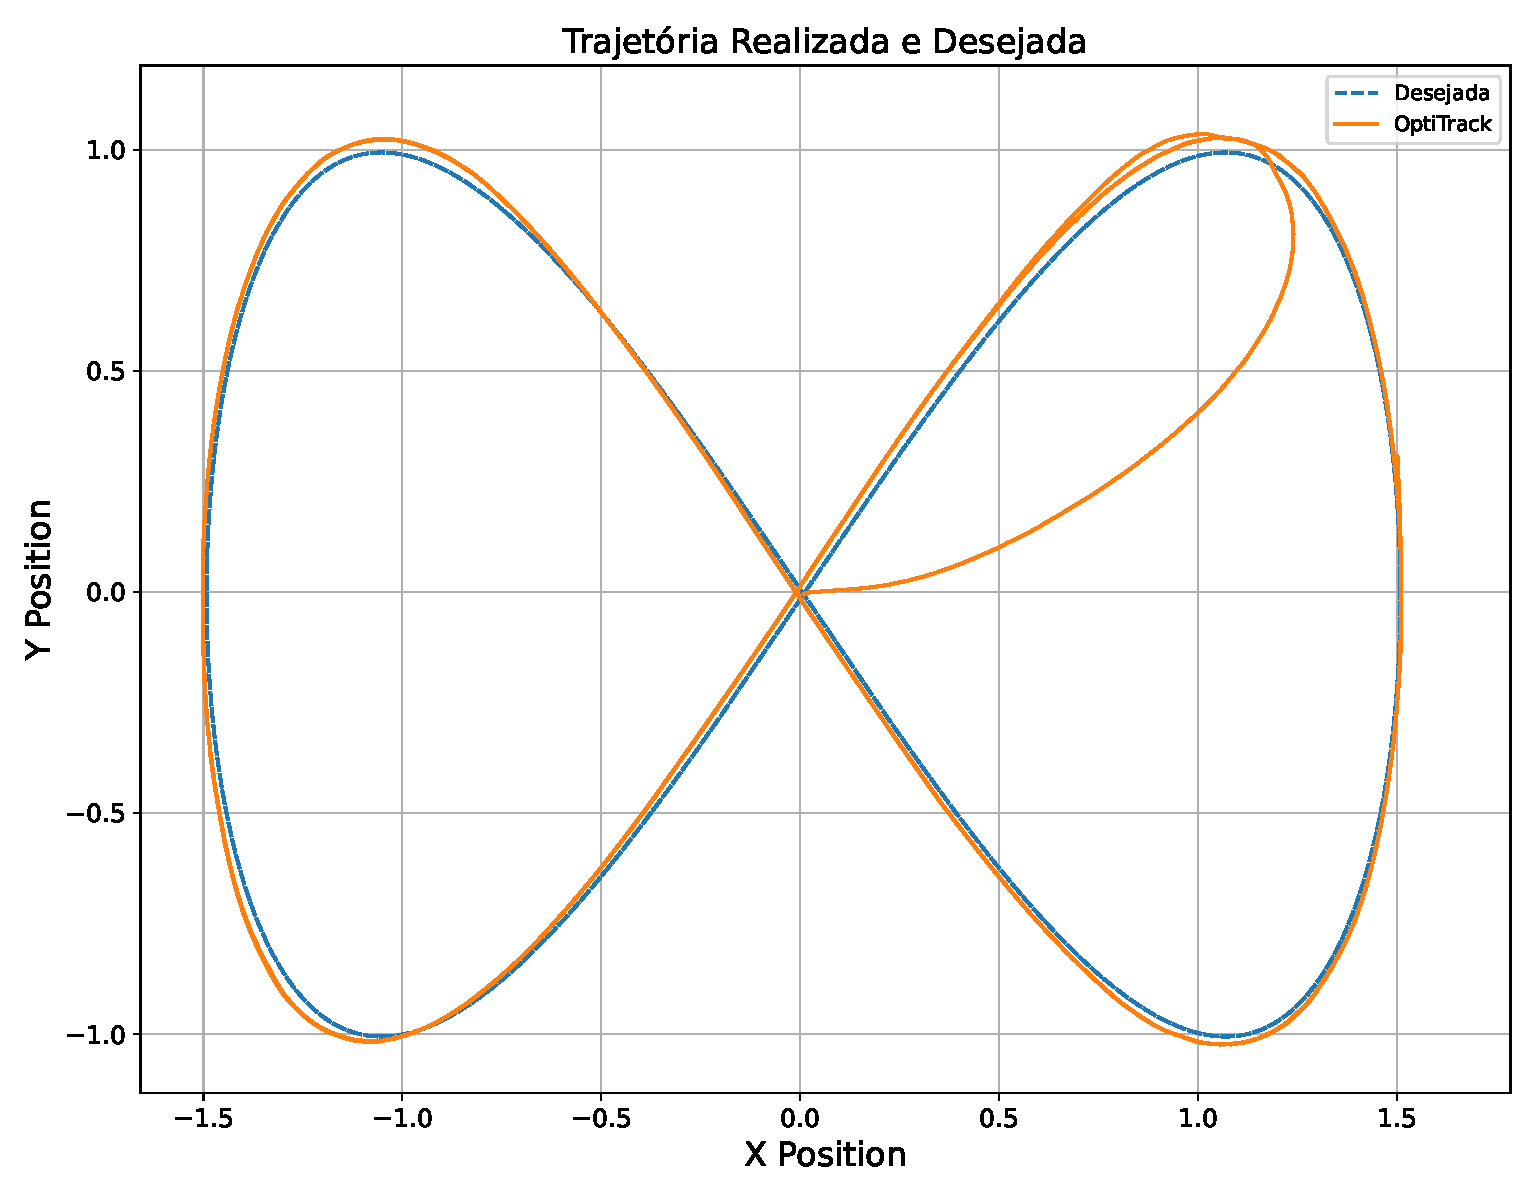
\includegraphics[width=0.8\linewidth]{img/Resultados/Exp2_VRPN_Control_LEMNISCATA/Trajetoria.pdf}
    \source
    \label{fig:Exp2_TrajetoriaVRPN}
\end{figure}

\begin{figure}[htb]
    \centering
    \caption{Experimento 2 - Comparação entre as posições registradas pelo OptiTrack e pela SLAM Toolbox durante o experimento}
    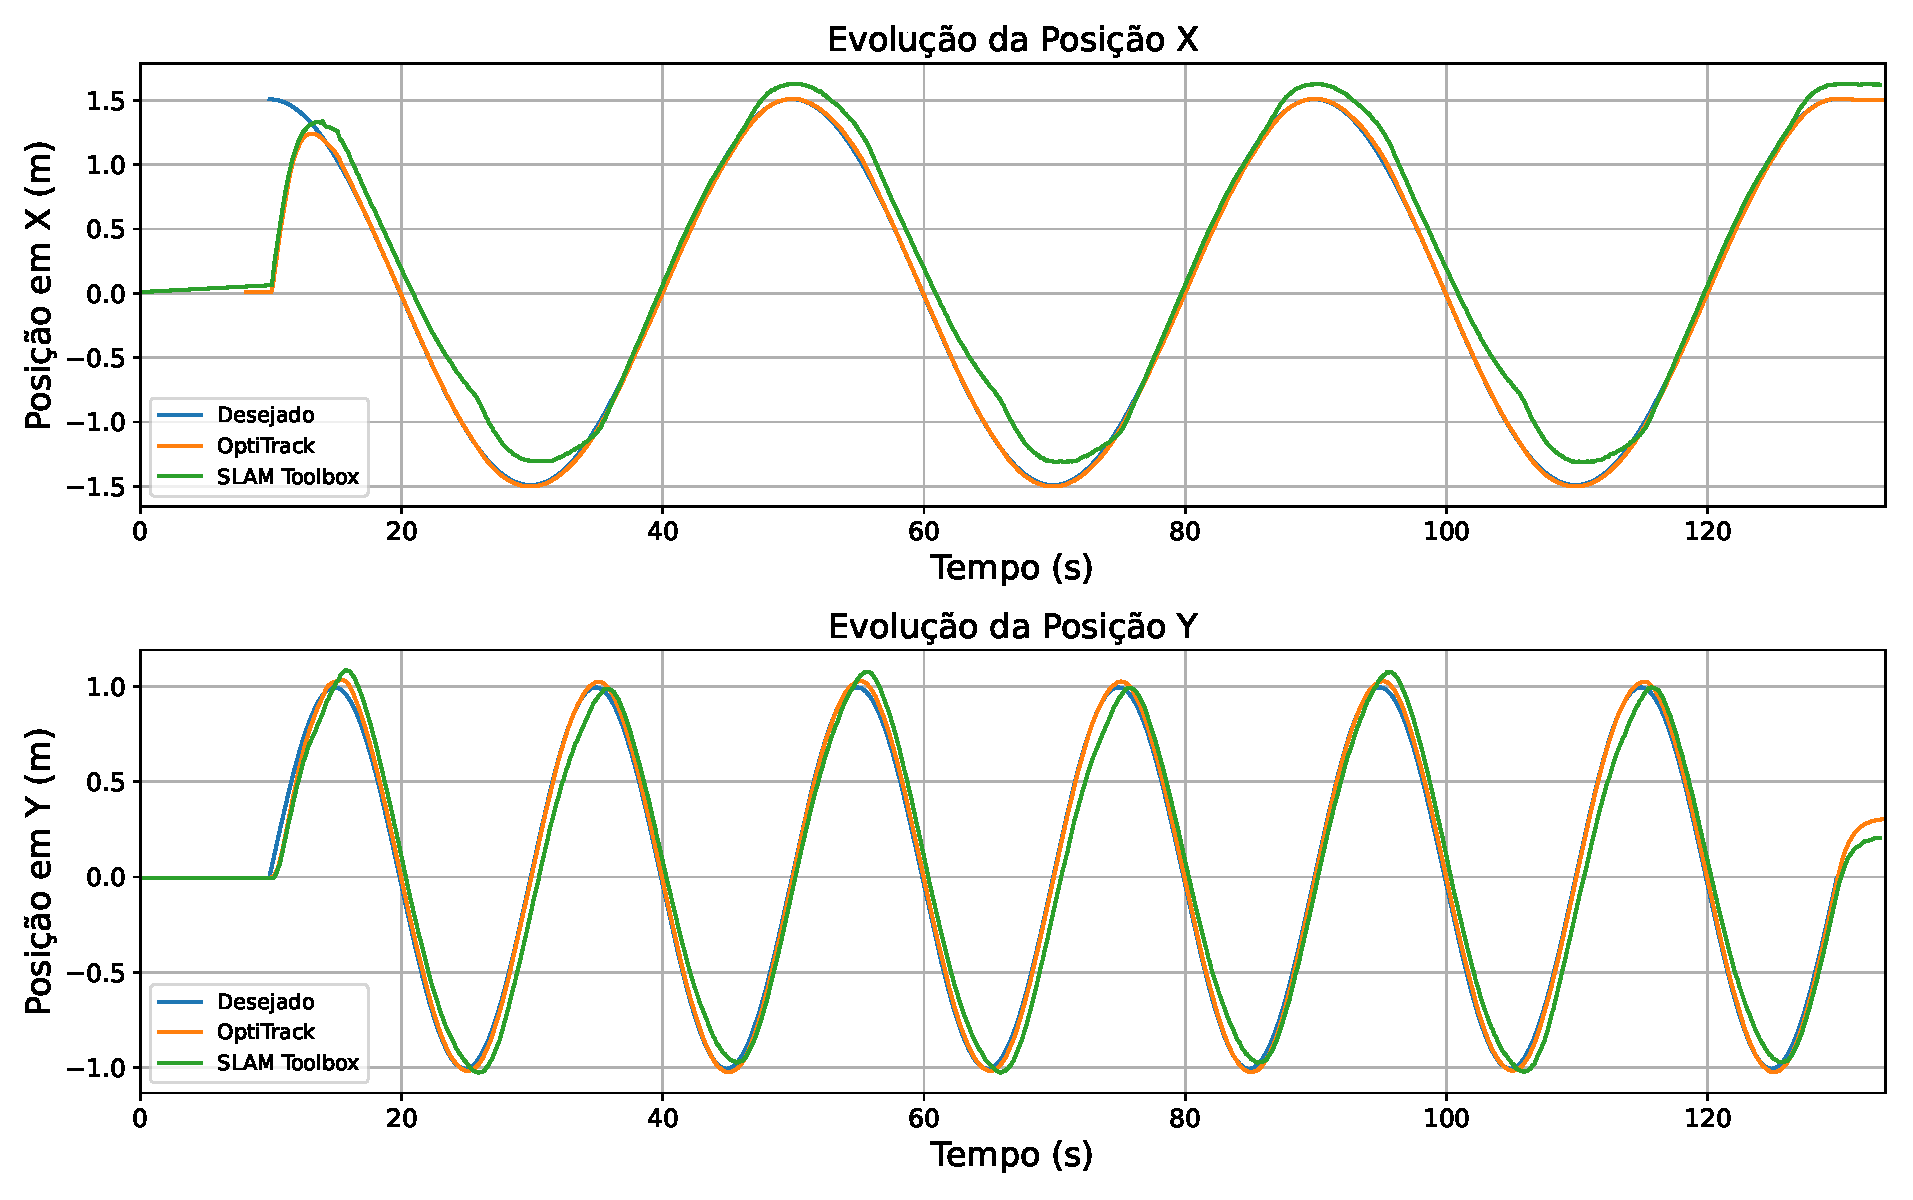
\includegraphics[width=\linewidth]{img/Resultados/Exp2_VRPN_Control_LEMNISCATA/pose_tempo.pdf}
    \source
    \label{fig:Exp2_Comparacao_Posicao_v_tempo}
\end{figure}


As Figuras \ref{fig:Exp3_Trajetoria} e \ref{fig:Exp3_Posicao_Tempo} mostram os resultados do terceiro experimento realizado, utilizando a pose obtida da SLAM Toolbox para controle do robô na tarefa de seguimento da trajetória \ASPASDUPLAS{CASA}. Observa-se na Figura \ref{fig:Exp3_Trajetoria} que o robô conseguiu seguir a trajetória desejada de modo satisfatório, porém com maiores erros de posição que no Experimento 1 (Figura \ref{fig:Exp1_Trajetoria_VRPN_LINEAR}) e um comportamento oscilatório em alguns trechos da trajetória.

\begin{figure}[htb]
    \centering
    \caption{Experimento 3: Trajetória desejada e realizada pelo robô}
    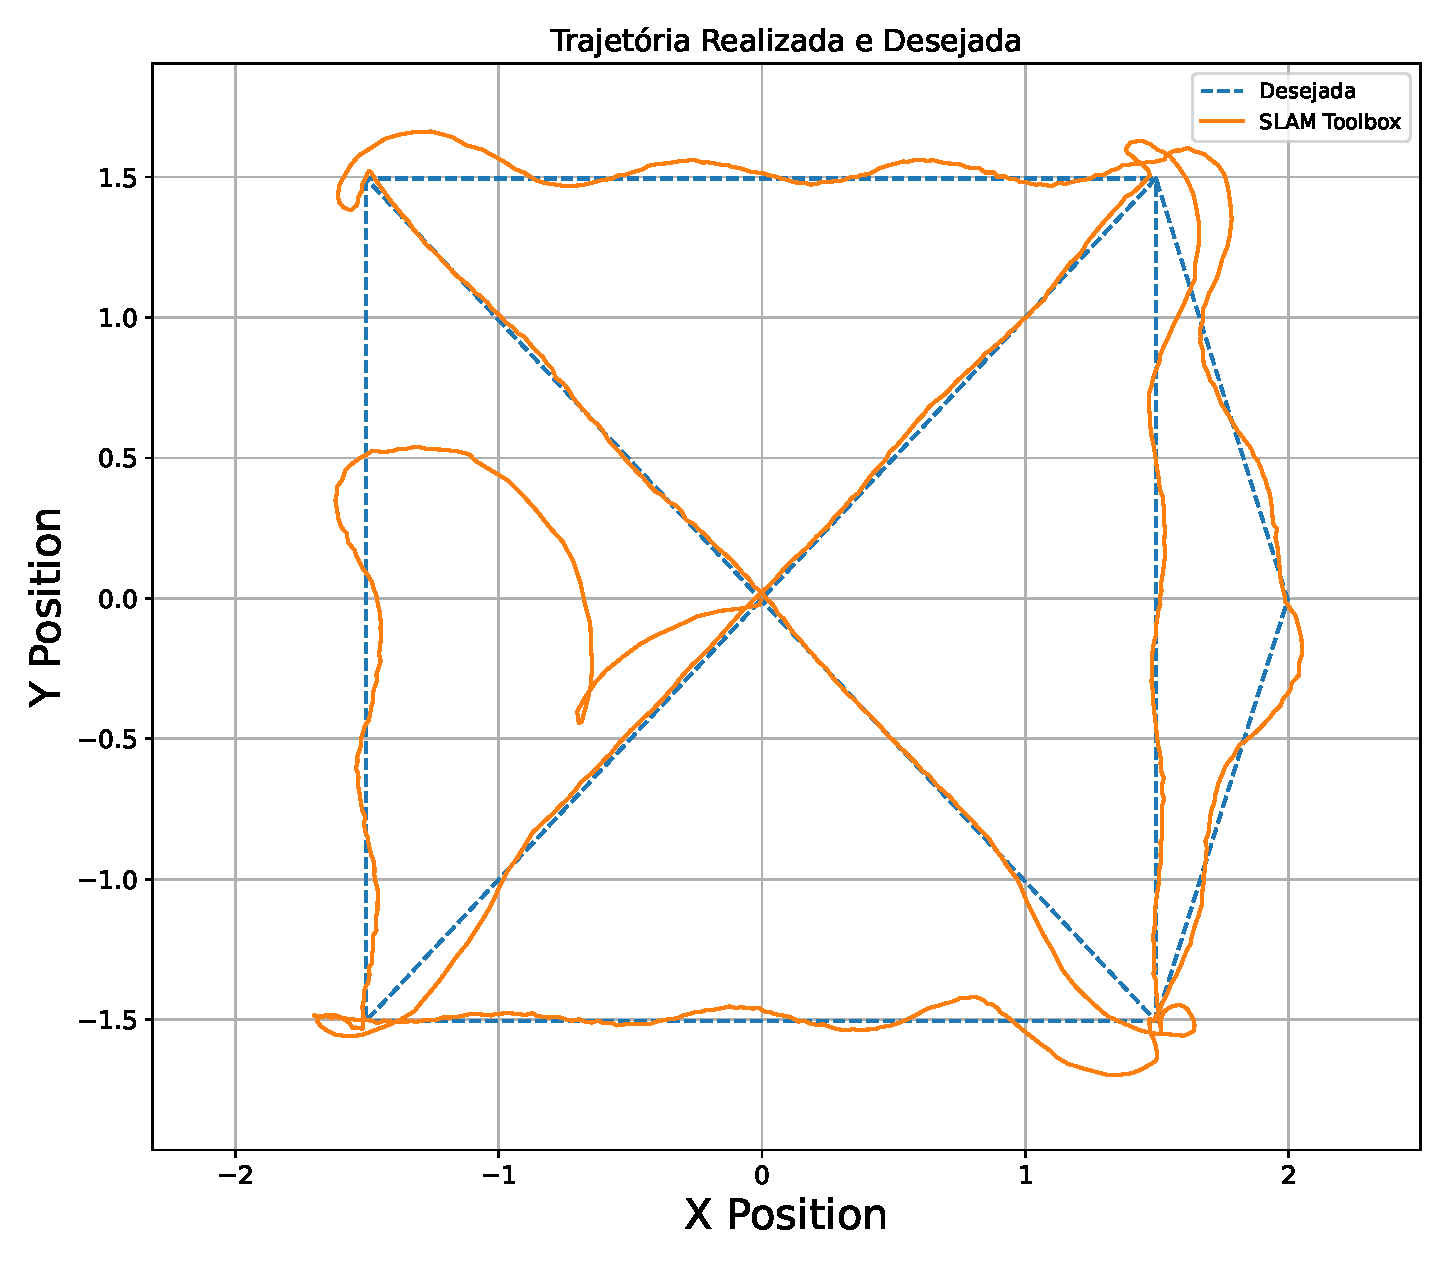
\includegraphics[width=0.7\linewidth]{img/Resultados/Exp3_SLAM_Control_LINEAR/trajetoria.pdf}
    \source
    \label{fig:Exp3_Trajetoria}
\end{figure}

\begin{figure}[htb]
    \centering
    \caption{Experimento 3: Comparação entre as posições registradas pelo OptiTrack e pela SLAM Toolbox durante o experimento}
    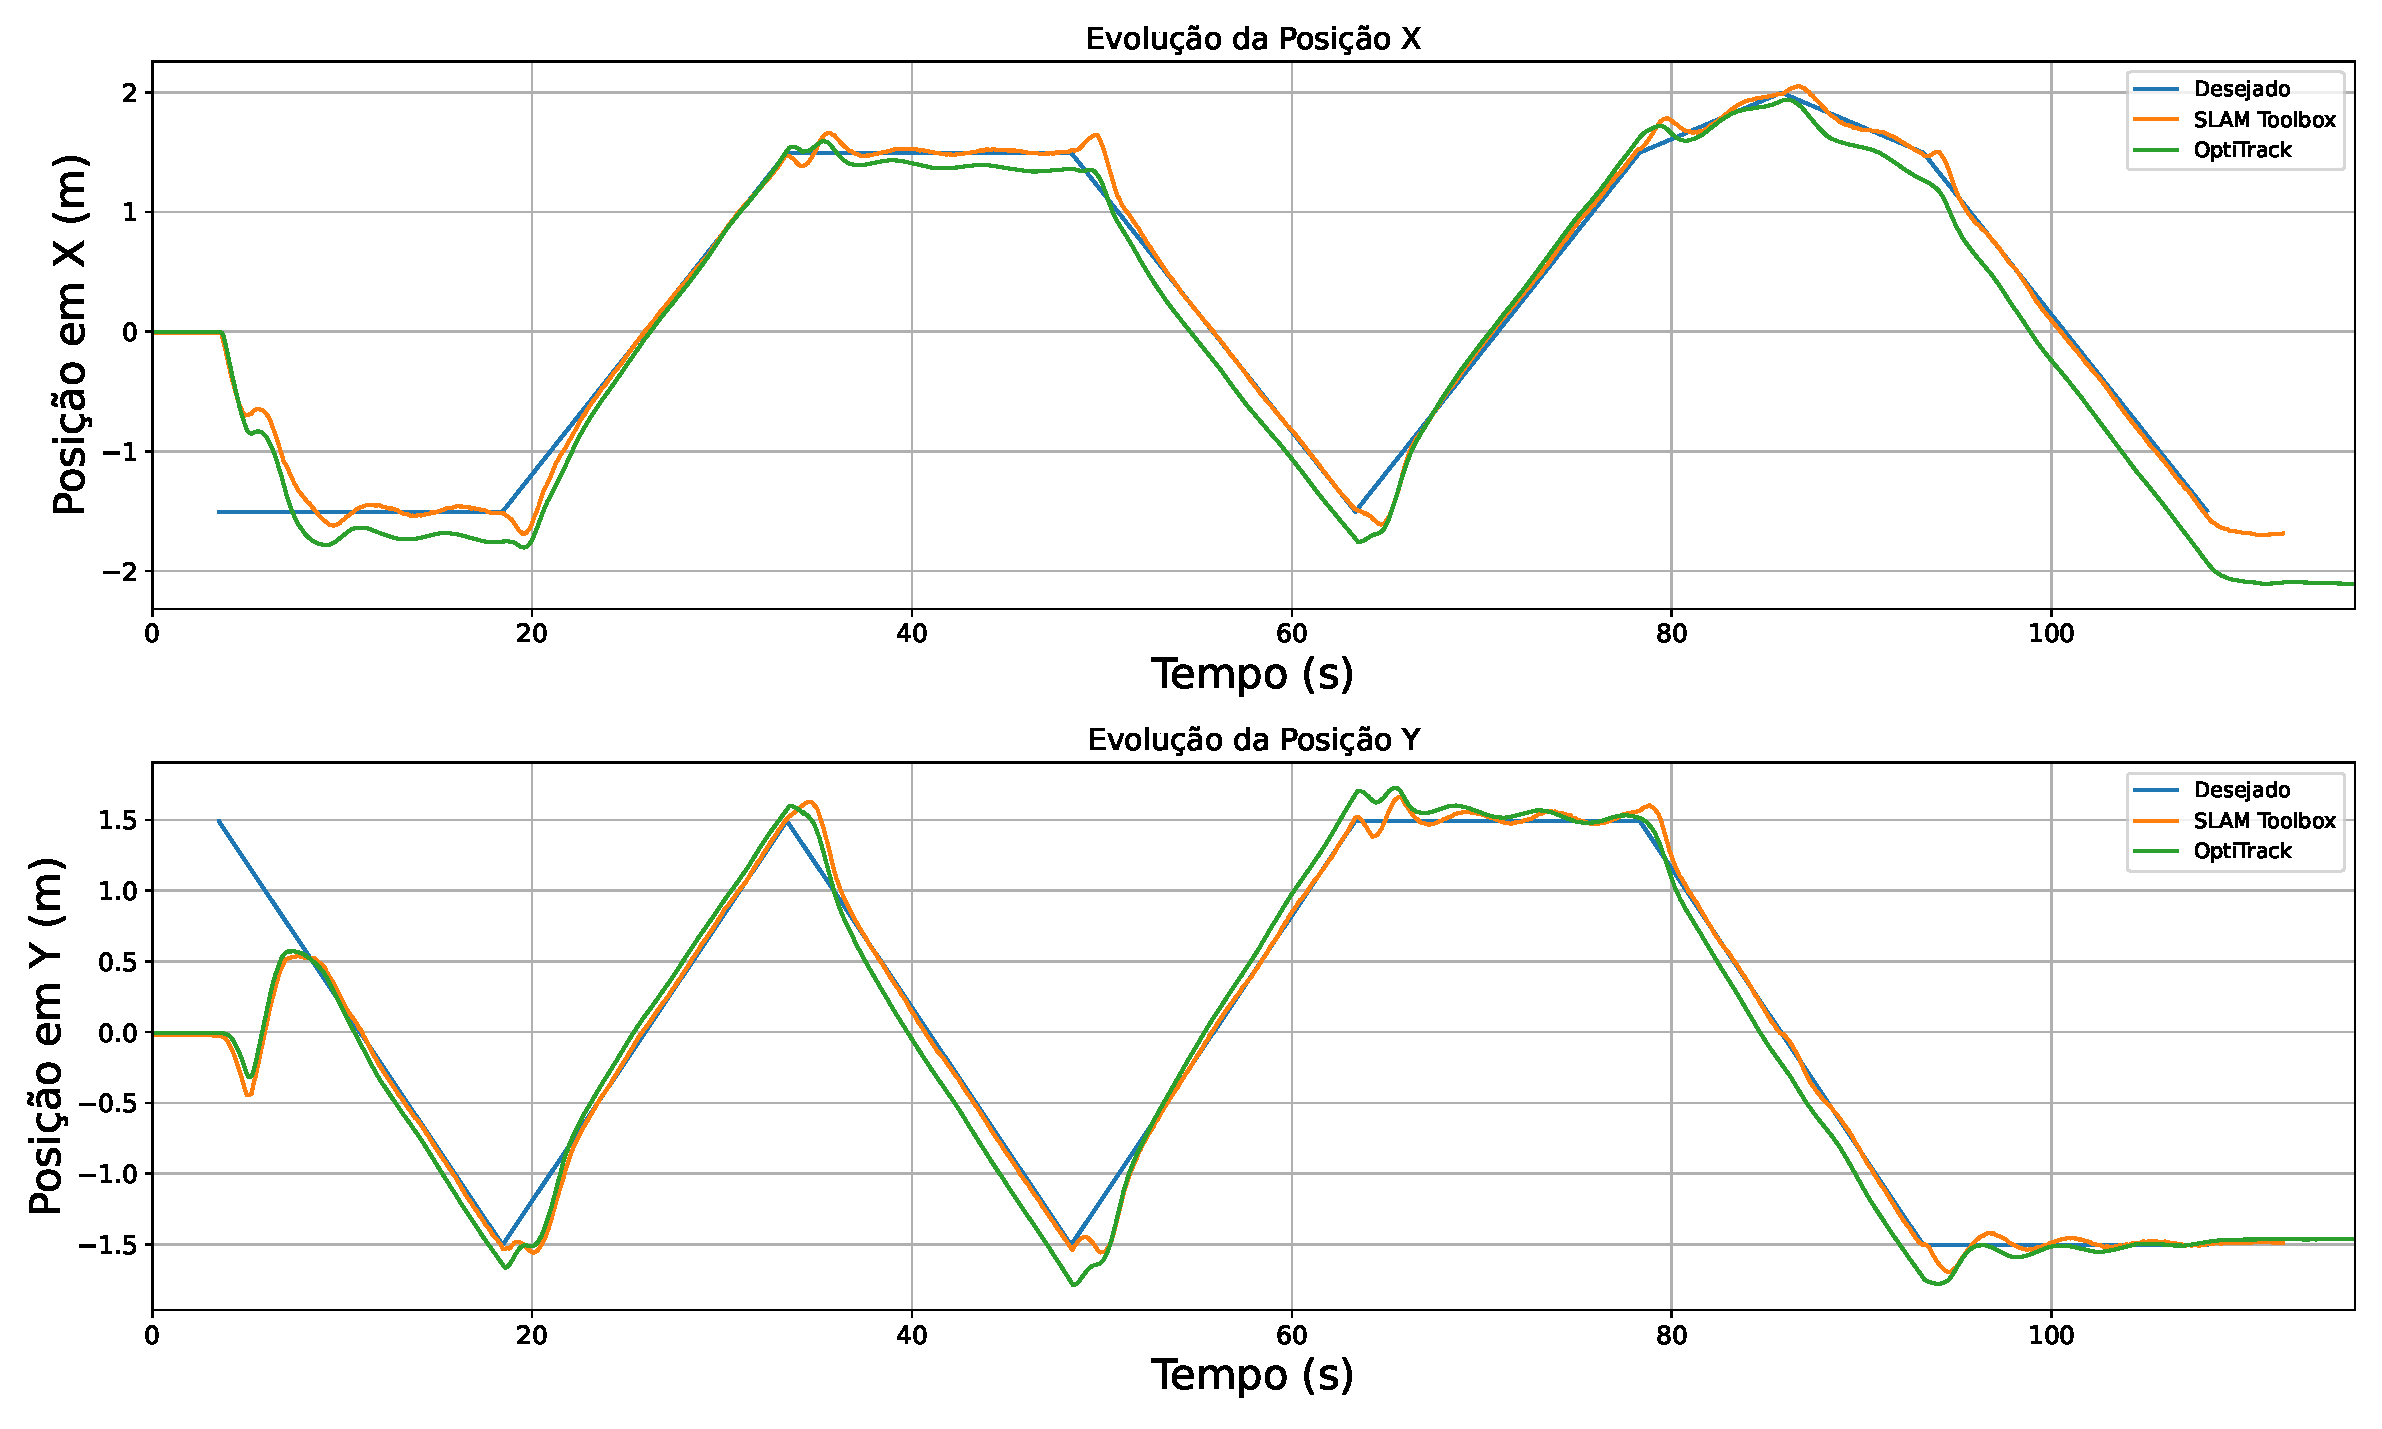
\includegraphics[width=\linewidth]{img/Resultados/Exp3_SLAM_Control_LINEAR/pose_tempo.pdf}
    \source
    \label{fig:Exp3_Posicao_Tempo}
\end{figure}


Na Figura \ref{fig:Exp3_Posicao_Tempo} mostra-se a evolução das posições no tempo, novamente com a posição equivalente ao sistema de câmeras OptiTrack aparecendo com o nome \ASPASIMPLES{vrpn} no gráfico e as posições obtidas da SLAM Toolbox com o nome \ASPASIMPLES{slam}. Nesta Figura também é possível notar o comportamento oscilatório durante o experimento, embora a diferença entre a posição do OptiTrack e da SLAM Toolbox não seja muito grande.



Os resultados do experimento 4 podem ser conferidos nas Figuras \ref{fig:Exp4_Trajetoria} e \ref{fig:Exp4_Posicao_Tempo}, em que a trajetória desejada foi a Lemniscata de Bernoulli da Equação \ref{eq:lemniscata}. Para este experimento em específico, definiu-se um tempo de experimento mais longo, de 15 minutos. Assim, podemos verificar o resultado da tarefa de localização do robô usando apenas a pose provinda da SLAM Toolbox como \textit{feedback} de controle durante um longo tempo. Apesar de notar-se um comportamento bastante oscilatório durante algumas etapas do experimento, o robô realizou a trajetória desejada durante todo o tempo do experimento, o que não seria possível se fosse utilizada apenas os dados da odometria do robô para executar a tarefa. A Figura \ref{fig:Exp4_Posicao_Tempo} mostra a evolução das posições durante o experimento.

\begin{figure}[htb]
    \centering
    \caption{Experimento 4: Trajetória desejada e realizada pelo robô}
    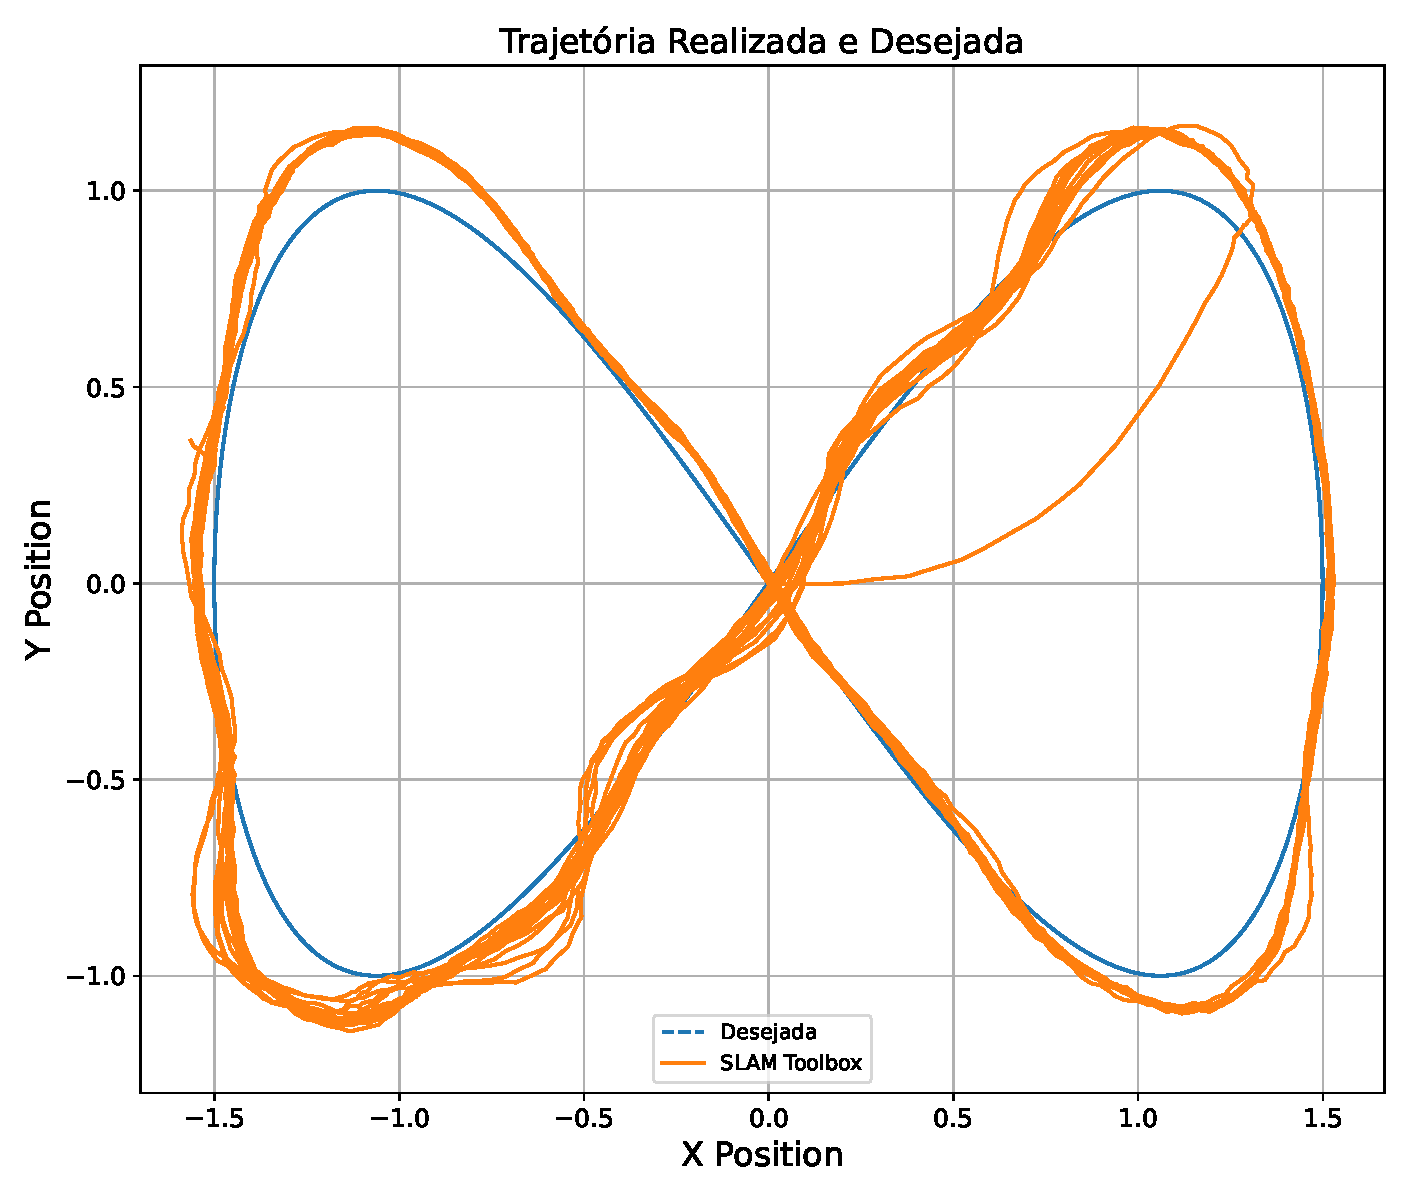
\includegraphics[width=\linewidth]{img/Resultados/Exp4_SLAM_Control_LEMNISCATA/Trajetoria.pdf}
    \source
    \label{fig:Exp4_Trajetoria}
\end{figure}


\begin{figure}[htb]
    \centering
    \caption{Experimento 4: Comparação entre as posições registradas pelo OptiTrack e pela SLAM Toolbox durante o experimento}
    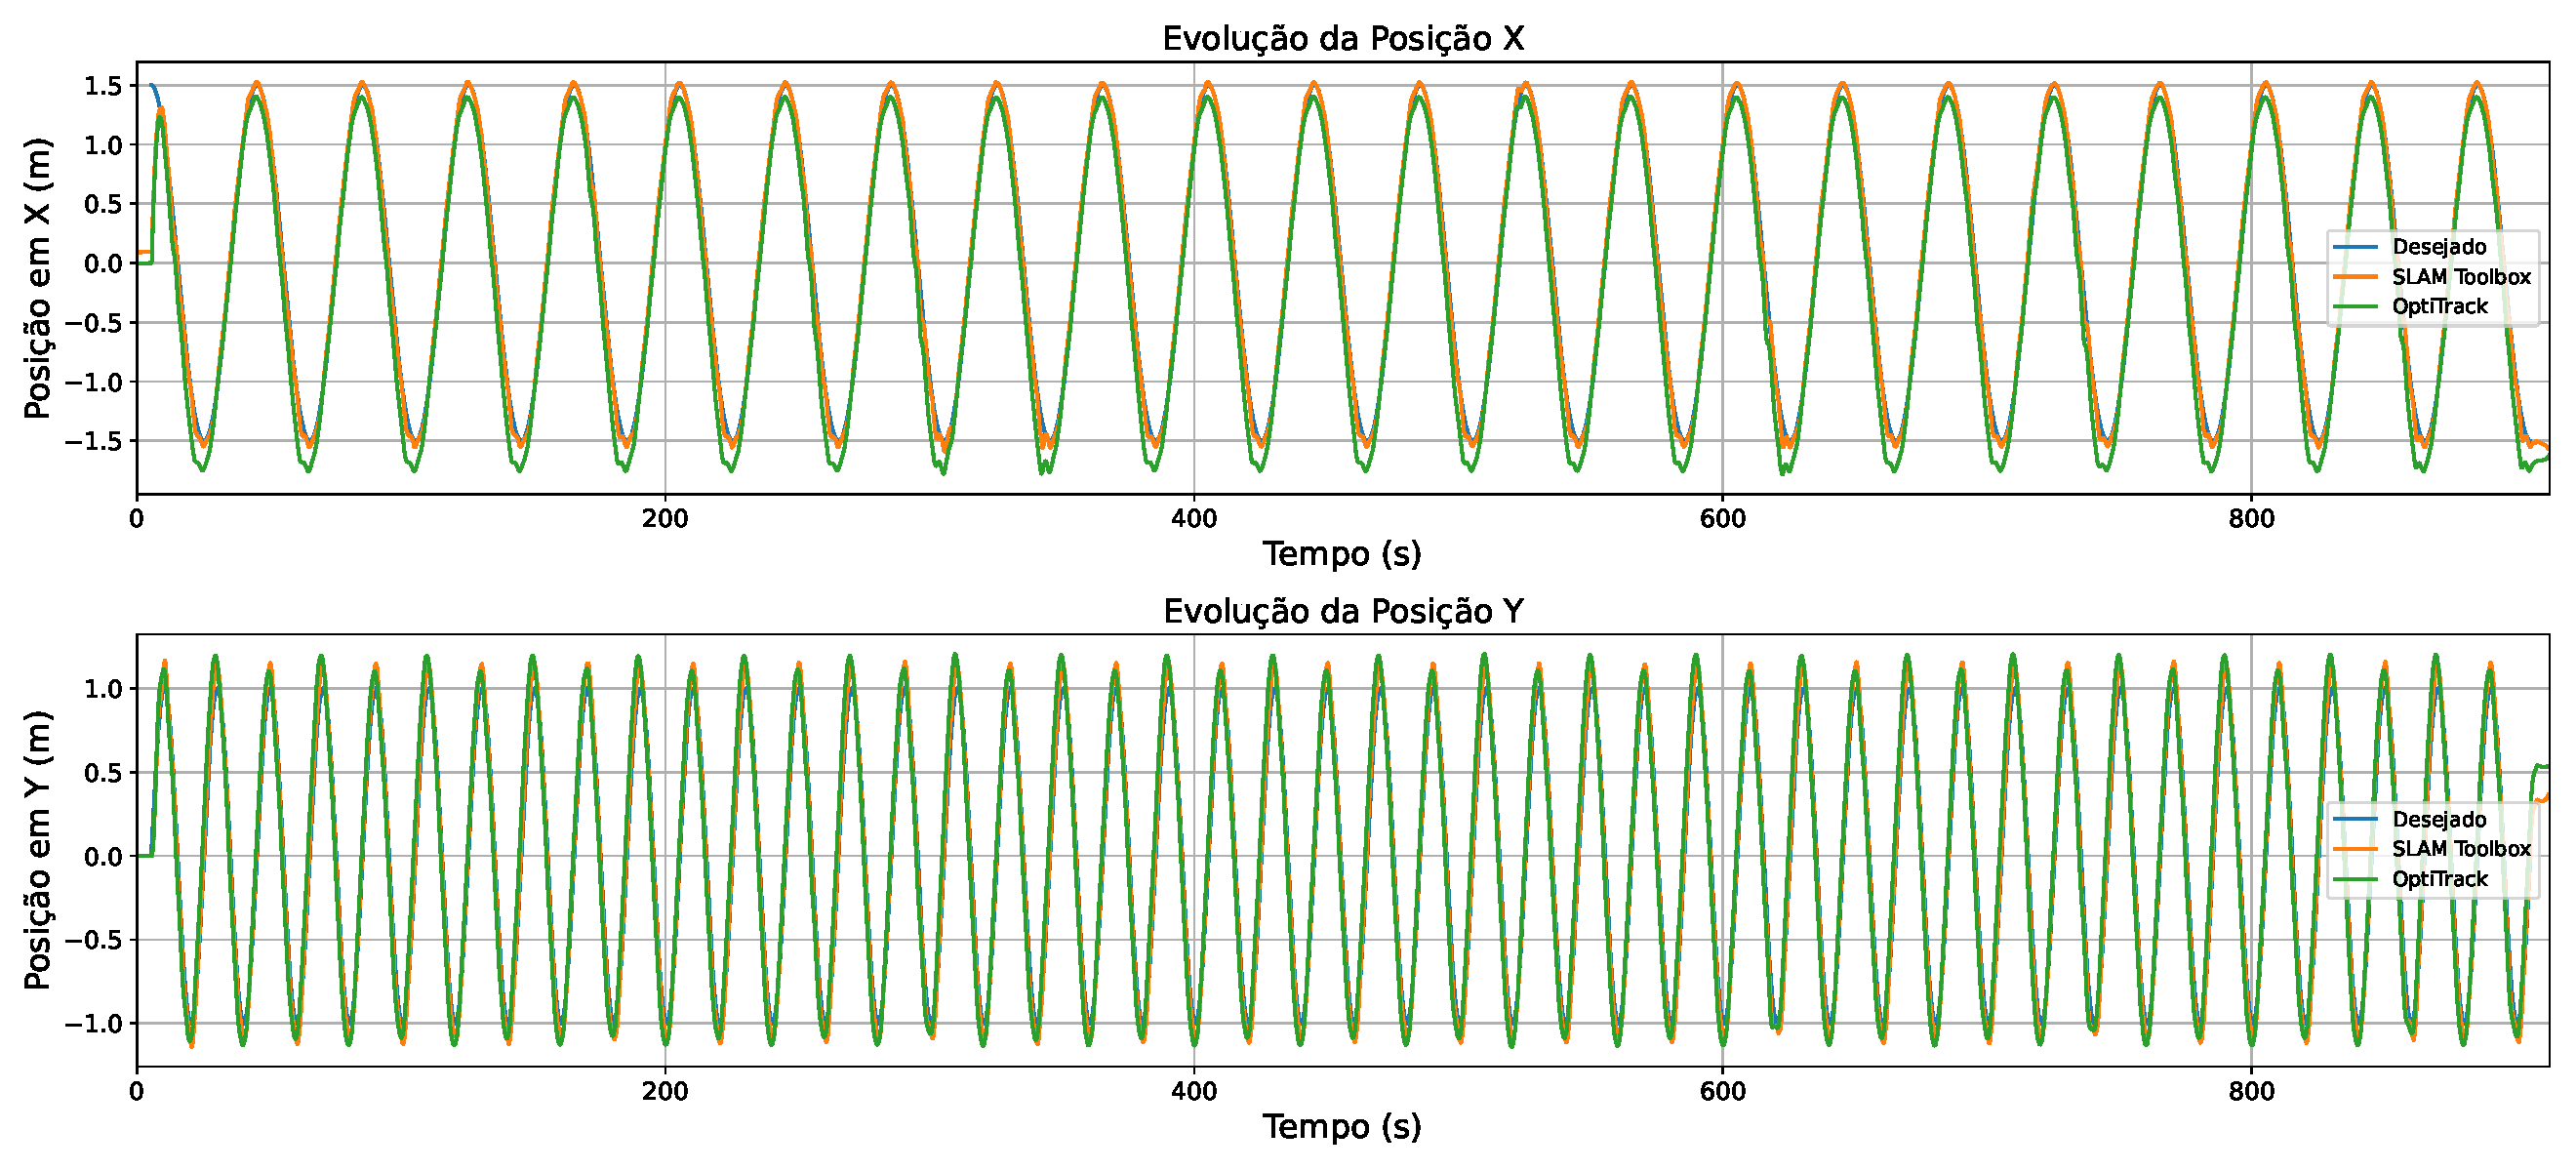
\includegraphics[width=\linewidth]{img/Resultados/Exp4_SLAM_Control_LEMNISCATA/pose_tempo.pdf}
    \label{fig:Exp4_Posicao_Tempo}
    \source
\end{figure}
\fi

%%%%%%%%%%%%%%%%%%%%%%%%%%%%%%%%%%%%%%%%%%%%%%%%%%%%%
%%%%%%%%%%%%%%%%%%%%%%%%%%%%%%%%%%%%%%%%%%%%%%%%%%%%%
%%%%%%%%%%%%%%%%%%%%%%%%%%%%%%%%%%%%%%%%%%%%%%%%%%%%%

\ifisTipoDocumento
    % PG
\else
    % TCC
    \chapter[Conclusão e Trabalhos Futuros]{Conclusão e Trabalhos Futuros}
    \label{Cap05}

% \begin{itemize}
%     \item \add{Síntese dos principais resultados e como eles atendem aos objetivos do projeto.}
%     \item \add{Reflexão sobre as vantagens e desvantagens da abordagem adotada (uso de biblioteca versus desenvolvimento completo do algoritmo).}
%     \item \add{Limitações do trabalho e sugestões para futuras melhorias ou pesquisas que possam superar os desafios encontrados.}
% \end{itemize}

% \section{Conclusão}

% \txr{Escrever a conclusão segundo os itens indicados a seguir.}

% \txr{OBJETIVO PRINCIPAL}
% O objetivo principal deste trabalho foi propor .....
% A técnica proposta é baseada fundamentalmente em ....
% Tal abordagem é motivada pelo ...

% \txr{DESCRIÇÃO DOS RESULTADOS}
% Como resultado, usando uma ...

% \txr{INTERPRETAÇÃO DOS RESULTADOS}
% A partir dos valores das métricas de...

% \txr{CONTRIBUIÇÃO DO TRABALHO}

% \section{Temas a serem pesquisados}

% \txr{Como trabalhos futuros: serão pesquisadas técnicas de ...}
% \txr{Além disso, futuramente ...}

% \txr{Finalmente, com o intuito de ....}

O presente trabalho apresentou o desenvolvimento de algoritmos de planejamento de rotas e controle de movimento para viabilizar a navegação autônoma de um robô móvel em tarefas de mapeamento. O principal objetivo foi explorar técnicas de controle cinemático e mapeamento a fim de permitir que o robô navegasse em um ambiente inicialmente desconhecido, localizando-se e construindo um mapa desse ambiente de forma autônoma. Para alcançar esse objetivo, foram implementados módulos essenciais: um controlador de trajetória para o robô móvel diferencial, rotinas de planejamento de trajetórias (definindo percursos a serem seguidos pelo robô) e a integração da biblioteca SLAM Toolbox para estimar a pose do robô e mapear o entorno. Como resultado, obteve-se um sistema capaz de guiar o robô de forma autônoma pelo ambiente de laboratório e realizou-se a validação da localização estimada pela biblioteca de SLAM com uma referência externa de alta precisão (sistema de câmeras OptiTrack).

Foram realizados experimentos em ambiente real para avaliar o desempenho dos algoritmos desenvolvidos. O robô percorreu duas trajetórias distintas pré-definidas no laboratório (uma sequência de segmentos retos, denominada "CASA", e uma curva fechada em formato de lemniscata de Bernoulli), sob duas configurações de obtenção de pose: (i) usando o sistema de câmeras OptiTrack como fonte de referência de alta precisão (ground truth) para a posição do robô; e (ii) usando exclusivamente a pose estimada pela SLAM Toolbox. Dessa forma, pôde-se comparar diretamente a qualidade da localização e o efeito desta na precisão do seguimento de trajetória.

Os resultados experimentais demonstraram que o sistema de controle e planejamento permitiu ao robô seguir as trajetórias desejadas em ambos os cenários de localização. Quando operando com a pose provida pelo OptiTrack (caso ideal), o robô apresentou boa aderência ao trajeto planejado, apresentando apenas erros modestos nos pontos de curvas mais fechadas e durante o início do deslocamento. Ao utilizar a pose estimada pela SLAM Toolbox, o robô também conseguiu completar as rotas, porém observou-se um aumento dos erros de seguimento e um leve comportamento oscilatório em certos trechos do percurso. Essa oscilação ficou especialmente evidente na trajetória em forma de lemniscata, sugerindo que imprecisões ou atrasos na atualização da pose pelo SLAM influenciaram o controlador. Apesar disso, ao comparar as trajetórias registradas pela SLAM Toolbox com aquelas medidas pelo OptiTrack, verificou-se que ambas permanecem próximas, indicando que a estimativa de posição obtida pela SLAM Toolbox é, em geral, confiável e possui erro limitado em relação à referência de alta precisão.

As principais limitações observadas concentram-se no desempenho dinâmico do robô durante o seguimento de trajetórias usando a localização por SLAM. O comportamento oscilatório e os erros mais acentuados em curvas indicam que o controlador poderia ser melhor ajustado ou complementado com técnicas de filtragem de ruído para lidar com a incerteza da pose estimada. 

Por fim, ressalta-se a decisão de utilizar a SLAM Toolbox em vez de desenvolver um algoritmo de SLAM próprio. Dado o alto nível de complexidade inerente a algoritmos de SLAM e considerando o tempo disponível, o uso dessa biblioteca consolidada do ROS mostrou-se adequado. A SLAM Toolbox provê mapeamento 2D eficiente e localização confiável, o que permitiu concentrar esforços no desenvolvimento dos controladores e na integração geral do sistema, evitando retrabalho em problemas já abordados por soluções existentes. Os resultados confirmam que essa escolha foi positiva, já que as estimativas de pose fornecidas pelo SLAM Toolbox foram consistentes ao longo dos testes, conforme verificado pela comparação com os dados do OptiTrack.

Como trabalhos futuros, diversas vertentes podem dar continuidade a este projeto. Uma direção promissora é estender o sistema para um cenário cooperativo com múltiplos robôs, incluindo robôs aéreos (drones) trabalhando em conjunto com o robô terrestre para acelerar o mapeamento e cobrir áreas maiores. Também se propõe aprimorar os controladores de movimento, seja por meio de sintonia mais refinada ou do uso de técnicas de controle avançadas, visando eliminar as oscilações observadas e melhorar a precisão de rastreamento da trajetória. Adicionalmente, a integração de algoritmos de planejamento global mais complexos permitiria que o robô utilizasse o mapa construído para planejar rotas ótimas e desviar de obstáculos de forma autônoma, em contraste às trajetórias fixas utilizadas neste trabalho. Essas evoluções tornariam o sistema mais robusto e eficiente, aproximando-o das exigências de aplicações reais de navegação autônoma cooperativa.
\fi

% --------------------------------------------------- %
%				Elementos Pós-Textuais				  %
% --------------------------------------------------- %

\postextual

% --------------------------------------------------- %
%				Referências Bibliográficas		      %
% --------------------------------------------------- %

\bibliography{BIBLIOGRAFIA/BIBLIOGRAFIA,BIBLIOGRAFIA/PG1_Mendeley,BIBLIOGRAFIA/Mendeley,BIBLIOGRAFIA/Education_Robotics,BIBLIOGRAFIA/LIVROS}

% --------------------------------------------------- %
%						Apêndices				  	  %
% --------------------------------------------------- %

%\begin{apendicesenv}
% Imprime uma página indicando o início dos apêndices
%\partapendices
% Insira os apêndices aqui em forma de capítulos
%\end{apendicesenv}

% --------------------------------------------------- %
%						Anexos						  %
% --------------------------------------------------- %

\begin{anexosenv}
%
%% Imprime uma página indicando o início dos anexos
% \partanexos
% \section{Dicas}
\label{sec:DicasEscrita}

Sobre \LaTeX
\begin{itemize}
\item 
\txr{\textbf{DICA:}}  Para trocar o ABNT para citação alfanumérica usar: 

\verb|\usepackage[alf]{abntex2cite}|

Este pacote esta localizado no inicio do documento \verb|PG_TEMPLATE.tex|.
\item 
\txr{\textbf{DICA:}} Para saber como fazer as referencias em LATEX ver: \url{https://www.overleaf.com/help/97-how-to-include-a-bibliography-using-bibtex}.

Ver os seguintes exemplos de citação
\begin{itemize}
\item 
Em \citeonline{zinkevichetal2010} os autores confirmam ...
\end{itemize}
\item 
\txr{\textbf{DICA:}} Para fazer comentários em blocos usar: \verb|CTRL + /| Obs: O barra usado no comando é o do teclado numérico.
\item 
\txr{\textbf{DICA:}} para usar variáveis matemáticas no texto usar o \verb|$|, por exemplo: na equação \verb|$x = \sqrt{\frac{a}{b}}$|, então, \verb|$y = \sin(x)$|.
\item 
\txr{\textbf{DICA:}} Em latex fica mais elegante usar $56 \times 56$ no lugar de 56 x 56.
\item 
\txr{\textbf{DICA:}} este template é configuravel para PG ou TCC, para trocar entre um formato e outro (respeitando o já escrito), deve-se fazer uso das variáveis logicas (localizadas nas linhas 129 e 130 do arquivo \verb|000_MAIN.tex|):
\begin{itemize}
\item 
\verb|\isTipoDocumentotrue %PG| descomentado para ativar o formato de PG.
\item 
\verb|\isTipoDocumentofalse %TCC| descomentado para ativar o formato de PG.
\end{itemize}
\end{itemize}

Exemplos de diferentes ambientes de equações:
% lembrar de usar \usepackage{amsmath} no preambulo
% mais ambientes em: https://pt.overleaf.com/learn/latex/Aligning_equations_with_amsmath

\begin{itemize}

    \item Equação centralizada e enumerada
        \begin{equation}
            \Delta = b^2-4 \cdot a \cdot c 
        \end{equation}

    \item Equação centralizada sem numeração
        \begin{equation*}
            \Delta = b^2 - 4 \cdot a \cdot c 
        \end{equation*}
        $$ \lim_{n\to\infty}x_n=0 $$
        $$ \textstyle \lim_{n\to\infty}x_n=0 $$
        
    \item Desenvolvimento de equações
        \begin{gather*}
            F_{cp} = \frac{m \cdot V^2}{R} \implies \frac{m \cdot V^2}{d \cdot \frac{\sqrt{3}}{3}} = \frac{G \cdot m^2}{d} \cdot \sqrt{3} \implies \frac{3 \cdot m \cdot V^2}{d \cdot \sqrt{3}} = \frac {G \cdot m^2 \cdot \sqrt{3}}{d^2}\\
            V^2 = \frac{G \cdot m}{2} \implies \boxed{V = \sqrt{\frac{G \cdot m}{d}}}
        \end{gather*}
    
    \item Equação no texto comprimida (textstyle)

        O limite é $\lim_{n\to\infty}x_n=0$.
        
        A integral é $ \int_a^b f(x) dx = \lim_{n \rightarrow
\infty} \sum_{i=0}^n f(x_i^*) \cdot \frac{b-a}{n}$.
        
        A relação $\frac{a}{b}$ vale 2.
    
    \item Equação no texto em tamanho normal (displaystyle)

        O limite é $\displaystyle \lim_{n\to\infty}x_n=0$.
        
        A integral é $ \displaystyle  \int_a^b f(x) dx = \lim_{n \rightarrow
\infty} \sum_{i=0}^n f(x_i^*) \cdot \frac{b-a}{n}$.
        
        A relação $\left (\dfrac{a}{b} \right )$ vale 2.
        
        A relação $ ( \dfrac{a}{b} )$ vale 2.

\end{itemize}
% Site para criar equações em Latex: https://www.codecogs.com/latex/eqneditor.php?lang=pt-br
% Site para simbolos matematicos Latex: https://latex.wikia.org/wiki/Main_page
% App para copiar códigos Latex de equações da internet: https://mathpix.com/

Exemplo de algoritmo:
% lembrar de usar \usepackage[linesnumbered]{algorithm2e} no preambulo
% mais estilos de algoritmos em: https://ctan.dcc.uchile.cl/macros/latex/contrib/algorithm2e/doc/algorithm2e.pdf

\begin{algorithm}[H]
    \SetAlgoLined
    \KwData{this text}
    \KwResult{how to write algorithm with \LaTeX2e }
        initialization\;
    \While{not at end of this document}{
        read current\;
    \eIf{understand}{
        go to next section\;
        current section becomes this one\;
    }{
        go back to the beginning of current section\;
    }
    \If{$\Delta$ == true}{
        show the match}
    }
    \caption{How to write algorithms}
\end{algorithm}





Sobre a escrita:
%http://posgraduando.com/dez-dicas-para-escrever-artigos-cientificos/
%https://wiki.sj.ifsc.edu.br/wiki/index.php/Dicas_para_escrita_de_texto_cient%C3%ADfico

\begin{itemize}
\item 
\txr{\textbf{DICA:}}  O trabalho científico deve ter um caráter formal e impessoal. Por conta disso, deve-se evitar a construção da oração na primeira ou terceira pessoa do singular. Assim, por exemplo, deve-se utilizar as seguintes expressões: \ASPADUPLA{conclui-se que}, \ASPADUPLA{percebe-se pela leitura do equipamento}, \ASPADUPLA{é válido supor}, \ASPADUPLA{ter-se-ia de dizer}, \ASPADUPLA{verificar-se-á} etc. Não é adequado, portanto, dizer: \ASPADUPLA{conforme vimos no item anterior}. Diz-se: \ASPADUPLA{conforme visto no item anterior}, ou, em vez de \ASPADUPLA{dissemos que}, \ASPADUPLA{foi dito que} etc.
\item 
\txr{\textbf{DICA:}} 
Evitar o uso de palavras que mostram significados abstratos (a menos que se efetue uma definição antes de seu uso), por exemplo: \ASPADUPLA{bom}, \ASPADUPLA{confiável}.
\item 
\txr{\textbf{DICA:}} Palavras em idioma estrangeiro necessariamente devem estar em italica, por exemplo: \textit{patch}, \textit{frame}, \textit{pipeline}.
\item 
\txr{\textbf{DICA:}} Para referir um termo em ingles usando siglas a formatação recomendada é: \verb|Nome em inglês - SIGLAS (tradução livre, Nome em português)|.
\item 
\txr{\textbf{DICA:}} Uma vez que declarada uma sigla ela deve ser usada por extenso no escrito.
\item 
\txr{\textbf{DICA:}} Toda Equação, Figura e Tabela no momento de ser referenciada deve iniciar em caixa alta, por exemplo: \verb|....na Equação ...|, \verb|....na Figura ...|, \verb|....na Tabela ...|. 
\item 
\txr{\textbf{DICA:}} Para referenciar uma Equação no texto usar o comando \verb|\eqref{}|. Por exemplo: 
\verb|.... na Equação \eqref{labelDaEquação} é ...|. 
\item 
\txr{\textbf{DICA:}} Toda Figura e Tabela deve ser referenciada no texto, para isso, deve-se usar o comando \verb|\ref{}|. Por exemplo: 
\verb|.... na Figura \ref{labelDaFigura} é mostrado ...|,  
\verb|....tal como é indicado na Tabela \ref{labelDaTabela} concluímos...|. 
\item 
\txr{\textbf{DICA:}} Os objetivos específicos devem casar completamente com o cronograma.
\item 
\txr{\textbf{DICA:}} Um bom escrito é um reflexo das leituras feitas sobre o tema em estudo, então, é prioritário ler bastante sobre o tema a dissertar.
\end{itemize}

Sobre as regras da correção do documento:
\begin{itemize}
\item 
\txr{\textbf{REGRA:}} Unicamente o orientador pode apagar as indicações/recomendações escritas em \txr{vermelho}. as \txr{DICAS} e \txr{COMENTARIO GERAL:} podem ser comentadas (usando \verb|\%|) depois de ser estudadas.
\item 
\txr{\textbf{REGRA:}} texto em \txb{AZUL}, indica modificações no escrito feitas pelo (co)orientador ou paragrafes com inconsistências, podem ser coloridas a \textbf{PRETO} uma vez estudado/corregido o problema.
\end{itemize}
% \section{Citação \textit{online}}

Segundo \citeonline{SpeechReview}, a partir da fala podemos extrair informações que permitem a identificação do locutor, da língua que está sendo falada,
% \section{Metodologia para o treinamento dos modelos neurais}
\label{sec:TrainDeepModel}

Redes neurais profundas são modelos computacionais complexos, com vários parâmetros a serem configurados e decisões a serem tomadas tanto na arquitetura quanto nos otimizadores e métricas utilizadas durante o treino. Além disso, ao contrário de modelos computacionais convencionais, problemas presentes na codificação de redes neurais na maioria das vezes causam falhas silenciosas, o que dificulta a sua detecção e correção. Para minimizar os problemas citados acima, aqui será seguida a metodologia apresentada por \citeonline{KarpathyRecipe:2019}.  Tal metodologia divide o treinamento de uma rede neural em seis etapas distintas, cada uma servindo a um propósito específico.
\begin{itemize}
\item 
\textbf{Primeira etapa}, efetuar uma inspeção do conjunto de dados usado para treinamento e validação, visualizando os dados e entendendo a sua distribuição. 
O principal objetivo desta etapa é encontrar problemas que possam existir, como dados duplicados, corrompidos, ou então tendências que existam meio aos dados e que possam prejudicar o treinamento. Além disso, esta etapa serve para construir uma intuição sobre quais técnicas podem funcionar ou não com os dados.
\item 
\textbf{Segunda etapa}, construir um modelo \textit{baseline}, para que seja possível testar um código inicial para realizar as etapas de treino e avaliação. 
Nessa etapa, o foco não é obter os melhores resultados, mas sim em garantir que os dados estão sendo lidos e transformados de maneira correta, assim como o bom funcionamento de outros componentes vitais para o sistema como métricas e funções de perda. O código deve ser o mais simples possível, para que existam o mínimo de fatores que possam introduzir falhas.
\item 
\textbf{Terceira etapa}, modificar o  modelo \textit{baseline} até chegar em um modelo sobre ajustado ao conjunto de dados, ou seja, ele apresenta melhores resultados nos dados de treino que em nos dados de validação. 
A impossibilidade de alcançar o sobre-ajuste com modelos mais complexos é um indício de problemas que existem durante o treinamento.
\item 
\textbf{Quarta etapa}, regularizar o modelo sobre ajustado para que generalize nas predições e assim ganhar desempenho nos dados de validação em troca de uma perda de acurácia nos dados de treino. 
Para isso, serão utilizadas técnicas conhecidas na literatura por reduzir o sobre-ajuste dos modelos.
\item 
\textbf{Quinta etapa}, efetuar a sintonia dos hiper-parâmetros de treino para obter o melhor resultado possível, 
Como existem diferentes hiper-parâmetros, com os mais diversos efeitos sobre o treino, 
é recomendado utilizar uma política de busca aleatória para se encontrar os melhores valores \cite{BergstraAndBengio:2012}.
\item 
\textbf{Sexta etapa}, utilizar \textit{ensembles} de modelos ou treinar por mais tempo como último recurso para melhorar o desempenho do sistema como um todo.
\end{itemize}
\end{anexosenv}

% --------------------------------------------------- %
%					Índice Remissivo				  %
% --------------------------------------------------- %
\phantompart
\printindex

\end{document}